% =============================================================================
% ENCICLOPÉDIA DE MÁQUINAS ROTODINÂMICAS — EDIÇÃO COMPLETA (volume único)
% -----------------------------------------------------------------------------
% ARQUIVO GERADO — não edite à mão.
% Fonte: Volume_0_Notacoes_e_Calculo.tex, Volume_I_Fundamentos.tex e
%        compressores.tex (os três continuam sendo os documentos canônicos).
% Gerador: scripts/gerar_edicao_completa.py
% Capa:    capa_edicao_completa.tex (essa sim, editável à mão)
%
% A numeração de capítulos, equações, figuras e tabelas de cada volume é
% preservada exatamente como na edição avulsa — o contador de seção é zerado na
% abertura de cada volume.
% =============================================================================
\documentclass[12pt,a4paper]{article}

\usepackage{cmap}
\usepackage[T1]{fontenc}
\usepackage[utf8]{inputenc}
\usepackage[brazilian]{babel}
\usepackage[expansion=false]{microtype}
\usepackage{amsfonts}
\usepackage{amsmath}
\usepackage{amssymb}
\usepackage{bm}
\usepackage{booktabs}
\usepackage{fancyhdr}
\usepackage{float}
\usepackage{geometry}
\usepackage{graphicx}
\usepackage{longtable}
\usepackage{pgfplots}
\usepackage{tabularx}
\usepackage{tikz}
\usepackage{titlesec}
\usepackage{hyperref}
\usepackage{xcolor}   % cores da capa (tikz já carrega, explícito por clareza)
\usetikzlibrary{patterns}
\pgfplotsset{compat=1.18}

\numberwithin{equation}{section}
\numberwithin{table}{section}
\numberwithin{figure}{section}

\geometry{margin=2.5cm, headheight=15pt}
\addtolength{\topmargin}{-0.5pt}
\emergencystretch=1em

\hyphenation{
  AGMA
  API
  ASHRAE
  ASME
  Auto-en-coder
  EKF
  En-gi-neer-ing
  FNO
  GUM
  IEC
  ISO
  LMTD
  MHE
  MPC
  NEMA
  NORSOK
  NTU
  Non-lin-ear
  Off-load-ing
  Off-shore
  PIML
  PINN
  PSA
  PSO
  RUL
  SHAP
  SPC
  VAE
  VFD
  VSD
  a-pro-xi-ma-ção
  a-pro-xi-ma-ções
  auto-en-coder
  blow-down
  blow-hole
  con-tí-nu-a
  con-tí-nuo
  di-fe-ren-ci-ais
  di-fe-ren-ci-al
  en-gi-neer-ing
  foul-ing
  head-er
  ins-tru-men-ta-ção
  ins-tru-men-ta-ções
  lo-ga-rit-mo
  lo-ga-rit-mos
  load
  me-câ-ni-ca
  me-câ-ni-cas
  non-lin-ear
  off-load-ing
  off-shore
  ro-to-di-nâ-mi-ca
  ro-to-di-nâ-mi-cas
  rub-bing
  shed-ding
  sur-ro-gate
  te-r-mo-di-nâ-mi-ca
  te-r-mo-di-nâ-mi-cas
  tim-ing
  tri-go-no-mét-ri-ca
  tri-go-no-mét-ri-cas
}

\hypersetup{
	colorlinks=true, linkcolor=black, citecolor=black, urlcolor=black,
	pdftitle={Enciclopédia de Máquinas Rotodinâmicas — Edição Completa},
	pdfauthor={Marcelo Moreira Mejias},
	pdfsubject={Volumes 0, I e II reunidos em volume único},
	pdfkeywords={máquinas rotodinâmicas, compressor de parafuso, offshore,
	             gêmeo digital, mecânica do contínuo, termofluidos, cálculo}
}

\pagestyle{fancy}
\fancyhf{}
\renewcommand{\sectionmark}[1]{\markboth{#1}{}}
\fancyhead[L]{\nouppercase{\leftmark}}
\fancyhead[R]{\thepage}
\renewcommand{\headrulewidth}{0.4pt}

\newcommand{\chapterword}{Capítulo}
\titleformat{\section}
	{\normalfont\Large\bfseries\raggedright}
	{\chapterword~\thesection}{1em}{}
	[\vspace{-0.5em}\rule{\textwidth}{0.4pt}]

\newcommand{\colecaotitulo}{Enciclopédia de Máquinas Rotodinâmicas}
\newcommand{\autorlivro}{Marcelo Moreira Mejias}
\newcommand{\revdatacompleta}{\today}

\begin{document}

% =============================================================================
% CAPA DA EDIÇÃO COMPLETA — Enciclopédia de Máquinas Rotodinâmicas
% -----------------------------------------------------------------------------
% Capa vetorial em TikZ puro, versionada no próprio .tex (mesma convenção das
% figuras dos Volumes 0 e I). Sem imagem externa: nada a licenciar, nada que
% possa faltar num clone, e escala sem perda em qualquer tamanho de impressão.
%
% Paleta herdada do projeto (scripts/gen_figuras.py e .streamlit/config.toml):
%   NAVY #1f3b57 — campo e traço técnico
%   BLUE #2b6cb0 — destaque frio
%   OURO #c8a24b — destaque quente, usado com parcimônia
%
% MOTIVO: o par de rotores de parafuso em ELEVAÇÃO, desenhado como os dois
% cilindros engrenados com suas hélices — 4 entradas no macho, 6 no fêmea, a
% proporção real da máquina do Volume II. A geometria é paramétrica (senoides
% recortadas pelo contorno do cilindro), não um contorno desenhado à mão: é o
% que separa desenho técnico de ilustração genérica. Uma primeira versão tentou
% o corte transversal com curvas de Bézier e produziu formas arredondadas sem
% leitura mecânica — descartada.
% =============================================================================

\definecolor{capaNavy}{HTML}{1F3B57}
\definecolor{capaNavyEsc}{HTML}{16293C}
\definecolor{capaBlue}{HTML}{2B6CB0}
\definecolor{capaClaro}{HTML}{DBE7F2}
\definecolor{capaPapel}{HTML}{F7F9FC}
\definecolor{capaOuro}{HTML}{C8A24B}

\begin{titlepage}
\thispagestyle{empty}
\begin{tikzpicture}[remember picture, overlay]

  % ---------------------------------------------------------------------------
  % Campo de fundo
  % ---------------------------------------------------------------------------
  \fill[capaNavy] (current page.south west) rectangle (current page.north east);

  % Faixa superior levemente mais escura: assenta a tipografia do topo sem
  % precisar de moldura.
  \fill[capaNavyEsc]
    (current page.north west) rectangle ([yshift=-62mm]current page.north east);

  % ---------------------------------------------------------------------------
  % MOTIVO — par de rotores em elevação, com hélices paramétricas
  % ---------------------------------------------------------------------------
  \begin{scope}[shift={([yshift=26mm]current page.center)}]

    % --- Rotor fêmea (atrás, 6 entradas) ---
    % Cada hélice é traçada PARAMETRICAMENTE só na face voltada ao observador
    % (fase de -90 a +90 graus, onde cos>0). Traçar a senoide inteira faria as
    % faces da frente e de trás se cruzarem, e o conjunto lê como treliça em
    % vez de rotor — foi o defeito da primeira versão.
    \begin{scope}[shift={(0,-1.52)}]
      \def\rF{1.28}    \def\cF{6.30}    \def\wF{2.05}
      \begin{scope}
        \clip (-\cF/2,-\rF) rectangle (\cF/2,\rF);
        \foreach \k in {0,...,5}{
          \foreach \n in {-2,-1,0,1,2}{
            \draw[capaBlue!75, line width=0.55pt]
              plot[domain={-90+360*\n}:{90+360*\n}, samples=34,
                   variable=\s, smooth]
              ({(\s*0.0174533 - \k*1.0472)/\wF}, {\rF*sin(\s)});
          }
        }
      \end{scope}
      \draw[capaBlue!90, line width=0.7pt] (-\cF/2,-\rF) -- (\cF/2,-\rF);
      \draw[capaBlue!90, line width=0.7pt] (-\cF/2, \rF) -- (\cF/2, \rF);
      \draw[capaBlue!90, line width=0.7pt] (-\cF/2,0) ellipse (0.30 and \rF);
      \draw[capaBlue!90, line width=0.7pt] ( \cF/2,0) ellipse (0.30 and \rF);
    \end{scope}

    % --- Rotor macho (à frente, 4 entradas, maior) ---
    \begin{scope}[shift={(0,1.18)}]
      \def\rM{1.66}    \def\cM{6.30}    \def\wM{1.40}
      \fill[capaNavy] (-\cM/2-0.34,-\rM) rectangle (\cM/2+0.34,\rM);
      \begin{scope}
        \clip (-\cM/2,-\rM) rectangle (\cM/2,\rM);
        \foreach \k in {0,...,3}{
          \foreach \n in {-2,-1,0,1,2}{
            \draw[capaClaro, line width=0.85pt]
              plot[domain={-90+360*\n}:{90+360*\n}, samples=40,
                   variable=\s, smooth]
              ({(\s*0.0174533 - \k*1.5708)/\wM}, {\rM*sin(\s)});
          }
        }
      \end{scope}
      \draw[capaPapel, line width=1.0pt] (-\cM/2,-\rM) -- (\cM/2,-\rM);
      \draw[capaPapel, line width=1.0pt] (-\cM/2, \rM) -- (\cM/2, \rM);
      \draw[capaPapel, line width=1.0pt] (-\cM/2,0) ellipse (0.38 and \rM);
      \draw[capaPapel, line width=1.0pt] ( \cM/2,0) ellipse (0.38 and \rM);
      % cotos de eixo
      \draw[capaPapel!75, line width=0.9pt] (-\cM/2-0.92,-0.16) rectangle (-\cM/2,0.16);
      \draw[capaPapel!75, line width=0.9pt] ( \cM/2,-0.16) rectangle ( \cM/2+0.92,0.16);
    \end{scope}

    % --- Eixos de centro: o vocabulário do desenho técnico ---
    \draw[capaOuro!70, line width=0.4pt, dash pattern=on 6pt off 2.5pt on 1pt off 2.5pt]
      (-4.60,1.18) -- (4.60,1.18);
    \draw[capaOuro!45, line width=0.4pt, dash pattern=on 6pt off 2.5pt on 1pt off 2.5pt]
      (-4.60,-1.52) -- (4.60,-1.52);
  \end{scope}

  % ---------------------------------------------------------------------------
  % Lombada simbólica: três faixas, na ordem de leitura 0 → I → II
  % ---------------------------------------------------------------------------
  \begin{scope}
    \coordinate (L) at ([xshift=15mm]current page.west);
    \fill[capaOuro]    ([yshift=48mm]L) rectangle ([xshift=4mm,yshift=112mm]L);
    \fill[capaBlue]    ([yshift=-20mm]L) rectangle ([xshift=4mm,yshift=44mm]L);
    \fill[capaBlue!60] ([yshift=-88mm]L) rectangle ([xshift=4mm,yshift=-24mm]L);

    \node[rotate=90, capaNavyEsc, font=\sffamily\bfseries\tiny, anchor=center]
      at ([xshift=2mm,yshift=80mm]L) {\textls[120]{VOLUME 0}};
    \node[rotate=90, capaPapel, font=\sffamily\bfseries\tiny, anchor=center]
      at ([xshift=2mm,yshift=12mm]L) {\textls[120]{VOLUME I}};
    \node[rotate=90, capaPapel, font=\sffamily\bfseries\tiny, anchor=center]
      at ([xshift=2mm,yshift=-56mm]L) {\textls[120]{VOLUME II}};
  \end{scope}

  % ---------------------------------------------------------------------------
  % Tipografia — bloco superior (identidade da coleção)
  % ---------------------------------------------------------------------------
  \node[anchor=north west, capaPapel, font=\sffamily\bfseries\Large, align=left]
    at ([shift={(30mm,-24mm)}]current page.north west)
    {\textls[90]{ENCICLOPÉDIA DE}\\[1.2mm]\textls[90]{MÁQUINAS ROTODINÂMICAS}};
  \draw[capaOuro, line width=2pt]
    ([shift={(30mm,-40mm)}]current page.north west) --
    ([shift={(58mm,-40mm)}]current page.north west);
  \node[anchor=north west, capaBlue!85, font=\sffamily\small]
    at ([shift={(30mm,-45mm)}]current page.north west)
    {Compressores de parafuso \textit{oil-free} para plantas offshore};

  % ---------------------------------------------------------------------------
  % Tipografia — bloco inferior (título e conteúdo)
  % ---------------------------------------------------------------------------
  \node[anchor=south west, capaPapel,
        font=\sffamily\bfseries\fontsize{46}{50}\selectfont]
    at ([shift={(30mm,74mm)}]current page.south west) {Edição Completa};

  \draw[capaPapel!45, line width=0.7pt]
    ([shift={(30mm,68mm)}]current page.south west) --
    ([shift={(180mm,68mm)}]current page.south west);
  \draw[capaOuro, line width=2.6pt]
    ([shift={(30mm,68mm)}]current page.south west) --
    ([shift={(66mm,68mm)}]current page.south west);

  % Os três volumes — numeral destacado à esquerda, título à direita
  \foreach \vy/\vnum/\vtit in {%
      56/0/{Notações e Cálculo Básico},
      42/I/{Fundamentos de Mecânica do Contínuo, Termofluidos e Sistemas de Medição},
      28/II/{Gêmeo Digital de Sistemas de Compressão Offshore}}{
    \node[anchor=north east, capaOuro, font=\sffamily\bfseries\large]
      at ([shift={(41mm,\vy mm)}]current page.south west) {\vnum};
    \node[anchor=north west, capaClaro, font=\sffamily\small, align=left,
          text width=132mm]
      at ([shift={(46mm,\vy mm)}]current page.south west) {\vtit};
  }

  % Autor e revisão
  \draw[capaPapel!25, line width=0.5pt]
    ([shift={(30mm,20mm)}]current page.south west) --
    ([shift={(180mm,20mm)}]current page.south west);
  \node[anchor=north west, capaPapel, font=\sffamily\bfseries\normalsize]
    at ([shift={(30mm,16mm)}]current page.south west) {\autorlivro};
  \node[anchor=north east, capaBlue!85, font=\sffamily\scriptsize]
    at ([shift={(180mm,16mm)}]current page.south west)
    {Volume único \,\textbullet\, Rev. \revdatacompleta};

\end{tikzpicture}
\end{titlepage}

% =============================================================================
% VERSO DA CAPA — nota sobre a edição
% =============================================================================
\newpage
\thispagestyle{empty}
\vspace*{\fill}
\begin{center}
	\begin{minipage}{0.78\textwidth}
		\small
		\textbf{Sobre esta edição.} Este volume único reúne, sem alteração de
		conteúdo, os três volumes da coleção \emph{Enciclopédia de Máquinas
		Rotodinâmicas}. A numeração de capítulos, equações, figuras e tabelas de
		cada volume é preservada exatamente como na edição avulsa: a
		Equação~5.5 do Volume~II continua sendo a Equação~5.5 aqui, e toda
		referência cruzada externa --- inclusive as citações de equação no
		código-fonte dos simuladores --- permanece válida.

		\vspace{0.8em}
		Os volumes avulsos continuam sendo os documentos canônicos. Esta edição
		é gerada a partir deles por
		\texttt{scripts/gerar\_edicao\_completa.py}, de modo que nunca divirja:
		qualquer correção feita num volume aparece aqui na próxima geração.

		\vspace{0.8em}
		\textbf{Como ler.} O Volume~0 é pré-requisito opcional --- quem domina o
		formalismo matemático pode começar direto no Volume~I. O Volume~I
		sustenta o Volume~II, mas cada capítulo foi escrito para ser consultável
		isoladamente. O sumário geral, a lista de figuras e a lista de tabelas
		cobrem os três volumes de uma vez.
	\end{minipage}
\end{center}
\vspace*{\fill}


% --- SUMÁRIO GERAL ---
\clearpage
\pagenumbering{roman}
\tableofcontents

\clearpage
\phantomsection
\addcontentsline{toc}{section}{Lista de Figuras}
\listoffigures

\clearpage
\phantomsection
\addcontentsline{toc}{section}{Lista de Tabelas}
\listoftables

\clearpage
\pagenumbering{arabic}


\clearpage
\thispagestyle{empty}
\phantomsection
\addcontentsline{toc}{part}{VOLUME 0 — Notações e Cálculo Básico}
\vspace*{\fill}
\begin{center}
	{\color{capaBlue}\sffamily\bfseries\Large\textls[200]{VOLUME 0}}\\[3mm]
	{\color{capaOuro}\rule{42mm}{2.2pt}}\\[9mm]
	{\huge\bfseries Notações e Cálculo Básico}\\[7mm]
	\begin{minipage}{0.68\textwidth}
		\centering\itshape\small Os pré-requisitos matemáticos da coleção, reunidos num percurso curto.
	\end{minipage}
\end{center}
\vspace*{\fill}
\clearpage

\setcounter{section}{0}
	% --- CAPA ---
	

	% --- DEDICATÓRIA ---
	\newpage
	\thispagestyle{empty}
	\vspace*{\fill}
	\begin{flushright}
		\textit{Aos que reaprendem o básico sem vergonha,}
		\textit{e aos que nunca o esqueceram.}
	\end{flushright}
	\vspace*{\fill}


% --- PREFÁCIO ---
\newpage
\section*{Prefácio}
\addcontentsline{toc}{section}{Prefácio — VOLUME 0}

Esta coleção pede do leitor um repertório mínimo: ler e manipular símbolos
matemáticos, operar com unidades, derivar, integrar e resolver as equações
diferenciais mais simples. Quem chega da formação recente talvez precise
apenas revisar; quem está há anos fora da sala de aula, ou quem nunca viu o
formalismo, precisa de um lugar para começar. O Volume~0 é esse lugar.

A intenção não é substituir os livros de cálculo e de física básica, mas
reunir, num único percurso curto, exatamente o que os Volumes~I e~II usam ---
nem mais, nem menos. Cada capítulo declara o que apresenta, mostra o que é
operacional e fecha com uma síntese que aponta onde a ferramenta reaparece
nos volumes seguintes. O leitor que domina o assunto de um capítulo pode
pulá-lo sem prejuízo; o leitor que duvida encontra aqui o mínimo necessário,
sem rodeios.

Nussenzveig~\cite{nussenzveig} cobre a física básica que antecede esta
notação; Guidorizzi~\cite{guidorizzi2013} cobre o cálculo em profundidade.
Para o aprofundamento, as referências de classe mundial são as de
Feynman~\cite{feynman1963} na física e de Apostol~\cite{apostol1967} e
Spivak~\cite{spivak2008} no cálculo. Este volume é o caminho curto entre
essas obras e a engenharia de máquinas.

% --- SUMÁRIO ---
\newpage

% --- LISTAS DE FIGURAS E TABELAS ---
\newpage
\newpage


%=============================================================================
% CAPÍTULO 1 — INTRODUÇÃO AO VOLUME 0
%=============================================================================
\clearpage
\section{Introdução ao Volume 0}\label{sec:v0-intro}

\subsection{Para quem é este volume}

Há dois leitores em mente. O primeiro é quem retoma os estudos depois de
anos de prática e percebe que o vocabulário simbólico esqueceu mais rápido
que o juízo físico --- sabe o que o problema pede, mas não lê mais a equação
com fluidez. O segundo é quem começa do zero relativo: tem firmeza em
aritmética e no raciocínio de causa e efeito, mas nunca sistematizou
funções, derivadas e integrais. Este volume serve aos dois. Para o primeiro,
é um relembrar ordenado; para o segundo, um aprender enxuto, com tudo o que
será cobrado depois --- e nada do que não será.

\subsection{O que este volume cobre --- e o que não cobre}

O recorte é definido pelo uso, não pela tradição. Estão aqui a notação
simbólica, as unidades e a análise dimensional, as funções elementares, os
vetores e o essencial de álgebra linear, o cálculo diferencial e integral em
uma e várias variáveis, as equações diferenciais ordinárias de primeira e
segunda ordem e as séries de aproximação. Não estão aqui a teoria dos
números reais, as demonstrações de existência e unicidade, a integração
avancada de funções especiais nem a teoria de espaços vetoriais: nada disso
aparece nos Volumes~I e~II, e portanto não tem lugar neste volume.

\subsection{Como usar este volume}

Os capítulos foram escritos para serem lidos em sequência, mas cada um pode
ser consultado isoladamente: todos usam a mesma notação, estabelecida no
Capítulo~\ref{sec:v0-notacao} e mantida sem exceção até o Volume~II. A
Tabela~\ref{tab:v0-c1-1} resume o papel de cada capítulo e o ponto dos
volumes seguintes em que ele reaparece.

\begin{table}[H]
\centering
\caption[Mapa do Volume 0 e suas pontes com os volumes I e II.]{%
Mapa do Volume 0: cada capítulo ensina uma ferramenta e indica onde ela é
usada nos Volumes I e II desta coleção.}
\label{tab:v0-c1-1}
\begin{tabularx}{\textwidth}{lXl}
\toprule
\textbf{Cap.} & \textbf{Ferramenta} & \textbf{Onde reaparece} \\
\midrule
\ref{sec:v0-notacao} & Notação e linguagem simbólica & Toda a coleção \\
\ref{sec:v0-unidades} & Unidades e análise dimensional & Toda a coleção \\
\ref{sec:v0-funcoes} & Funções elementares e gráficos & Caps. 2 a 9 do Vol.~I \\
\ref{sec:v0-vetores} & Vetores e álgebra linear & Caps. 2, 4 e 7 do Vol.~I \\
\ref{sec:v0-derivadas} & Cálculo diferencial & Leis de taxa, Vol.~I \\
\ref{sec:v0-integrais} & Cálculo integral & Balanços, Vol.~I \\
\ref{sec:v0-edo} & Equações diferenciais & Modelagem dinâmica, Vol.~II \\
\ref{sec:v0-series} & Séries e aproximações & Linearização e erros, Vols.~I e~II \\
\bottomrule
\end{tabularx}
\end{table}

Quem já domina um capítulo avança sem culpa; quem duvida resolve os exemplos
à mão --- nenhum passo deste volume exige computador.

\subsection{Exercícios resolvidos}

\textbf{Exercício 1.1 (navegação pelo mapa).} Um colega relata: ``a
temperatura da carcaça do meu compressor está subindo há duas semanas, sem
ninguém mexer em nada''. Quais capítulos deste volume preparam a leitura
desse sintoma nos volumes seguintes, e em que ordem?

\emph{Resolução.} A Tabela~\ref{tab:v0-c1-1} responde. A temperatura que
sobe é uma \emph{taxa}, então o Capítulo~\ref{sec:v0-derivadas} é o
instrumento central; a análise do porquê vai usar \emph{balanços} de
calor, do Capítulo~\ref{sec:v0-integrais}; a resposta da carcaça ao calor
generado é uma equação diferencial, do
Capítulo~\ref{sec:v0-edo}; e a comparação de grandezas de escalas
muito diferentes (W contra $^\circ$C) pede o Capítulo~\ref{sec:v0-unidades}. A
notação do Capítulo~\ref{sec:v0-notacao} atravessa todos eles. Ordem
sugerida de revisão: \ref{sec:v0-notacao} $\rightarrow$
\ref{sec:v0-unidades} $\rightarrow$ \ref{sec:v0-derivadas} $\rightarrow$
\ref{sec:v0-integrais} $\rightarrow$ \ref{sec:v0-edo}.
Nenhum número foi calculado aqui --- o exercício é usar o mapa.


%=============================================================================
% CAPÍTULO 2 — NOTAÇÃO E LINGUAGEM SIMBÓLICA
%=============================================================================
\clearpage
\section{Notação e Linguagem Simbólica}\label{sec:v0-notacao}

\subsection{Por que a notação importa}

A notação é a gramática da física aplicada. Uma equação como
$\tau = J_p\,\alpha$ só pode ser lida de cor porque cada símbolo tem papel
fixo: letras em itálico representam grandezas que variam, letras em romano
representam nomes e funções, operadores têm formas próprias. Quem internaliza
essa gramática lê equações como frases; quem não internaliza decora
desenhos. Este capítulo fixa a gramática usada em toda a coleção.

\subsection{Fontes: itálico para variáveis, romano para nomes}

A convenção seguida em todos os volumes é a dos textos clássicos de
matemática aplicada:

\begin{itemize}
\item \textbf{Itálico} para variáveis e grandezas: $x$, $T$ (temperatura),
$p$ (pressão), $t$ (tempo), $\omega$ (velocidade angular).
\item \textbf{Romano} para operadores, funções com nome e unidades:
$\mathrm{d}x$ (diferencial), $\mathrm{sen}$, $\mathrm{ln}$, $\mathrm{exp}$,
$\max$, e as unidades $\mathrm{m}$, $\mathrm{s}$, $\mathrm{Pa}$.
\item \textbf{Negro} para vetores e matrizes: $\bm{v}$, $\bm{F}$,
$\bm{\nabla}T$.
\end{itemize}

O diferencial escreve-se $\mathrm{d}$ romano para distinguir o operador da
variável: $\mathrm{d}t$ lê-se ``um pedacinho de $t$''. O número
$\mathrm{e} \approx 2{,}71828$ (base dos logaritmos naturais) e a unidade
imaginária $\mathrm{i}$ seguem a mesma regra --- escrita $\mathrm{j}$ na
engenharia elétrica, para não colidir com a corrente $i$; é a convenção do
Capítulo~7 do Volume~I.

\subsection{Operadores e símbolos de uso geral}

A Tabela~\ref{tab:v0-c2-1} reúne os operadores que aparecem em toda a
coleção. Nenhum deles é opcional: todos serão usados nos volumes seguintes.

\begin{table}[H]
\centering
\caption[Operadores matemáticos e seu significado.]{%
Operadores matemáticos usados em toda a coleção.}
\label{tab:v0-c2-1}
\begin{tabularx}{\textwidth}{lX}
\toprule
\textbf{Símbolo} & \textbf{Significado} \\
\midrule
$=$ & igualdade exata \\
$\approx$ & aproximadamente igual (dentro de uma tolerância declarada) \\
$\equiv$ & identidade, definição ou equivalência por hipótese \\
$:= $ & ``é definido como'' (a igualdade aponta da definição para o nome) \\
$\propto$ & proporcional a (igual a menos uma constante) \\
$\rightarrow$, $\to$ & tende a; ou mapeamento de função \\
$\sum$, $\prod$ & somatório e produtório de uma sequência \\
$\mathrm{d}/\mathrm{d}t$ & derivada em relação ao tempo (taxa instantânea) \\
$\partial/\partial x$ & derivada parcial em relação a $x$ \\
$\nabla$ & gradiente (vetor das derivadas parciais) \\
$\int_a^b$ & integral definida entre $a$ e $b$ \\
$\Delta$ & variação finita (ex.: $\Delta T = T_2 - T_1$) \\
$\delta$ & variação infinitesimal ou incerteza, conforme o contexto \\
$\lfloor\cdot\rfloor$, $\lceil\cdot\rceil$ & piso e teto \\
$\forall$, $\exists$ & ``para todo'', ``existe'' \\
\bottomrule
\end{tabularx}
\end{table}

Duas distinções valem reforço. A variação finita $\Delta x = x_2 - x_1$ é um
número comum entre dois estados; o diferencial $\mathrm{d}x$ é um pedacinho
de variável dentro de um processo de limite --- a integral é feita deles. E
a distinção entre $\approx$ e $\equiv$: a primeira admite erro, que deve ser
declarado ou estimável; a segunda não admite erro nenhum, apenas convenção.

\subsection{Letras gregas}

A engenharia de máquinas usa intensivamente as letras gregas, e a mesma
letra costuma ter uso dominante em cada área. A Tabela~\ref{tab:v0-c2-2}
lista as que aparecem nos Volumes~I e~II com seu papel principal.

\begin{table}[H]
\centering
\caption[Letras gregas e seu uso dominante nesta coleção.]{%
Letras gregas mais usadas na coleção e seu significado dominante.}
\label{tab:v0-c2-2}
\begin{tabularx}{\textwidth}{llX}
\toprule
\textbf{Min.} & \textbf{Mai.} & \textbf{Uso dominante} \\
\midrule
$\alpha$ & & aceleração angular; coeficiente de expansão \\
$\beta$ & & razão de compressão volumétrica \\
$\gamma$ & $\Gamma$ & razão de calores específicos $c_p/c_v$ \\
$\delta$ & $\Delta$ & variação finita; folga (Volume II) \\
$\varepsilon$ & & deformação; eficiência alternativa; rugosidade \\
$\zeta$ & & fator de amortecimento \\
$\eta$ & & eficiência \\
$\theta$ & $\Theta$ & ângulo; temperatura reduzida \\
$\lambda$ & $\Lambda$ & comprimento de onda; autovalor \\
$\mu$ & & viscosidade dinâmica; coeficiente de atrito \\
$\nu$ & & viscosidade cinemática; frequência natural \\
$\rho$ & & massa específica \\
$\sigma$ & $\Sigma$ & tensão; somatório \\
$\tau$ & & torque; tensão de cisalhamento \\
$\phi$ & $\Phi$ & razão de fluxo; função \\
$\psi$ & $\Psi$ & função de corrente (fluidos) \\
$\omega$ & $\Omega$ & velocidade angular; $\Omega$ é a unidade ohm \\
\bottomrule
\end{tabularx}
\end{table}

Quando uma letra servir a dois usos, o texto declara qual vale na ocasião;
o Volume~I adota essa regra desde seu primeiro capítulo.

\subsection{Índices, expoentes e adornos}

Grandeza nenhuma anda sozinha: a coleção escreve $p_1$ e $p_2$ para pressões
em dois pontos, $T_{h,i}$ para temperatura de entrada do fluido quente, e
$\dot{m}$ (ponto por cima) para vazão mássica --- o ponto codifica
``por unidade de tempo''. Adornos têm significado fixo: linha por cima
($\bar{x}$) para média, til ($\tilde{x}$) para valor adimensionalizado,
chapéu ($\hat{x}$) para estimativa. Subscritos romanos nomeiam
($c_p$ = calor específico \emph{a pressão constante}); subscritos itálicos
indexam ($x_i$, o $i$-ésimo valor).

\subsection{Síntese: premissas e ligação com os volumes seguintes}

Este capítulo não postulou física nenhuma: fixou apenas a escrita. As
convenções aqui estabelecidas --- fontes, operadores, letras gregas,
adornos --- valem sem exceção do Capítulo~\ref{sec:v0-unidades} deste volume
até o capítulo final do Volume~II. Quando o Volume~I escreve
$\bm{\nabla}T$, é o gradiente desta Tabela~\ref{tab:v0-c2-1}; quando escreve
$\eta$, é a eficiência desta Tabela~\ref{tab:v0-c2-2}.

\subsection{Exercícios resolvidos}

\textbf{Exercício 2.1 (papel tipográfico).} Na equação $\tau = J_p\,\alpha$,
identifique o papel tipográfico de cada símbolo e explique por que o
subscrito de $J_p$ é romano.

\emph{Resolução.} $\tau$ (torque), $J_p$ (momento polar de inércia) e
$\alpha$ (aceleração angular) são grandezas que variam --- por isso
itálico. O subscrito $p$ é romano porque \emph{nomeia} e não indexa: ele
não enumera valores $J_1, J_2, \dots$; ele diz de \emph{qual} momento de
inércia se trata (polar). Pela regra do capítulo, subscrito romano nomeia,
subscrito itálico indexa.

\textbf{Exercício 2.2 (variação finita × taxa).} Uma tabela registra
$\Delta p = p_{out} - p_{in} = 12\ \mathrm{kPa}$ num intervalo de 1 h e,
numa outra coluna, $\mathrm{d}p/\mathrm{d}t = -0{,}8\ \mathrm{kPa/min}$. Os
dois números contradizem um ao outro?

\emph{Resolução.} Não --- medem coisas diferentes. $\Delta p$ é variação
finita entre dois estados, um número comum. $\mathrm{d}p/\mathrm{d}t$ é
uma taxa instantânea, o limite do quociente quando o intervalo
encolhe. Ambos podem ser verdadeiros ao mesmo tempo: a pressão terminou
12 kPa mais alta do que começou e, num instante específico, caía a
0,8 kPa por minuto.


%=============================================================================
% CAPÍTULO 3 — UNIDADES, DIMENSÕES E ORDEM DE GRANDEZA
%=============================================================================
\clearpage
\section{Grandezas, Unidades e Análise Dimensional}\label{sec:v0-unidades}

\subsection{Grandezas e unidades: o número e o rótulo}

Toda grandeza física é um número multiplicado por uma unidade:
``$p = 7{,}0\ \mathrm{bar}$'' significa $7{,}0$ vezes a unidade bar.
O número isolado não significa nada físico --- 7,0 de quê? --- e a unidade
isolada tampouco. A primeira disciplina deste capítulo é nunca separar os
dois: escrever a unidade junto a cada valor, em todos os passos de todos os
cálculos.

As unidades usadas em toda a coleção são as do Sistema Internacional (SI),
resumidas na Tabela~\ref{tab:v0-c3-1} com as grandezas de interesse desta
obra. Unidades fora do SI aparecem apenas quando a prática industrial as
impõe --- o bar para pressão e o rpm para rotação ---, e sempre com conversão
explícita na primeira ocorrência.

\begin{table}[H]
\centering
\caption[Unidades do SI usadas nesta coleção.]{%
Grandezas e unidades do SI usadas nesta coleção.}
\label{tab:v0-c3-1}
\begin{tabularx}{\textwidth}{llX}
\toprule
\textbf{Grandeza} & \textbf{Símbolo} & \textbf{Unidade SI (abrev.)} \\
\midrule
comprimento & $L$ & metro (m) \\
massa & $m$ & quilograma (kg) \\
tempo & $t$ & segundo (s) \\
corrente elétrica & $I$ & ampère (A) \\
temperatura & $T$ & kelvin (K) \\
\midrule
força & $F$ & newton (N = kg\,m\,s$^{-2}$) \\
pressão & $p$ & pascal (Pa = N\,m$^{-2}$) \\
energia, trabalho & $E$, $W$ & joule (J = N\,m) \\
potência & $P$ & watt (W = J\,s$^{-1}$) \\
\bottomrule
\end{tabularx}
\end{table}

Os prefixos do SI multiplicam as unidades por potências de dez. Os que
aparecem na coleção são poucos e devem ser lidos de cor:
$\mathrm{k}$ (quilo, $10^3$), $\mathrm{M}$ (mega, $10^6$),
$\mathrm{G}$ (giga, $10^9$), $\mathrm{m}$ (mili, $10^{-3}$),
$\mu$ (micro, $10^{-6}$). Assim, $1\ \mathrm{kW} = 10^3\ \mathrm{W}$ e
$1\ \mu\mathrm{m} = 10^{-6}\ \mathrm{m}$. Dois cuidados permanentes: o
prefixo $\mathrm{m}$ minúsculo é mili, enquanto $\mathrm{M}$ maiúsculo é
mega --- seis ordens de grandeza de diferença; e prefixos não se combinam
(diz-se $\mathrm{kg}$, nunca ``$\mathrm{k}\mu\mathrm{g}$'').

\subsection{Homogeneidade dimensional}

Uma equação física só pode somar grandezas de mesma dimensão: não se soma
metros a segundos, nem joules a watts. Essa exigência, chamada
\textbf{homogeneidade dimensional}, é o verificador mais barato que existe:
qualquer equação que some termos de dimensões diferentes está errada, antes
de qualquer cálculo numérico. As dimensões fundamentais da mecânica são
comprimento $[L]$, massa $[M]$ e tempo $[t]$; toda grandeza mecânica se
decompõe nelas. A Equação~\eqref{eq:v0-c3-1} mostra a verificação para a
pressão:

\begin{equation}\label{eq:v0-c3-1}
[p] = \frac{[F]}{[A]} = \frac{[M]\,[L]\,[t]^{-2}}{[L]^2}
    = [M]\,[L]^{-1}\,[t]^{-2}.
\end{equation}

A análise dimensional faz mais que detectar erro: ela \emph{descobre} a forma
das relações. Se um período de oscilação depende só de uma massa $m$ e de
uma rigidez $k$ (dimensão $[M][t]^{-2}$), a única combinação com dimensão de
tempo é $\sqrt{m/k}$ --- a constante numérica a análise não dá, mas a
dependência inteira ela dá. O Volume~I usa esse argumento nos grupos
adimensionais do Capítulo~4, e o Volume~II o repete no dimensionamento
preliminar.

\subsection{Notação científica e ordem de grandeza}

A notação científica escreve qualquer número como
$m \times 10^n$, com $1 \le m < 10$ e $n$ inteiro:
$c = 3{,}00 \times 10^8\ \mathrm{m/s}$. Ela existe para dois motivos
operacionais. O primeiro é comparar: saber se um resultado é
$2 \times 10^{-3}$ ou $2 \times 10^{3}$ é saber se a conta está no
universo certo, antes de conferir qualquer dígito. O segundo é o
\textbf{estimativa de ordem de grandeza}: arredondar cada fator para a
potência de dez mais próxima e multiplicar as potências. Uma bomba de
$3{,}2\ \mathrm{kW}$ operando $6{,}5\ \mathrm{h/dia}$ gasta, em ordem de
grandeza, $10^3 \times 10^1 = 10^4\ \mathrm{Wh}$ por dia --- dez vezes mais
que mil e dez vezes menos que cem mil. Quem estima antes de calcular nunca
confunde kW com MW.

\subsection{Algarismos significativos e arredondamento}

Um instrumento que lê $7{,}0\ \mathrm{bar}$ afirma algo mais forte que um
que lê $7\ \mathrm{bar}$: afirma que o valor está entre $6{,}95$ e
$7{,}05$. Os \textbf{algarismos significativos} codificam essa afirmação:
o último dígito escrito é o incerto, todos os anteriores são firmes. As
regras operacionais são poucas:

\begin{itemize}
\item na multiplicação e divisão, o resultado tem tantos significativos
  quanto o fator com menos significativos;
\item na adição e subtração, o resultado tem tantas casas decimais quanto
  o termo com menos casas decimais;
\item o arredondamento é feito no resultado final, nunca nos passos
  intermediários --- guardar dígitos extras durante a conta não é
  desonestidade, é precaução.
\end{itemize}

\subsection{Exercícios resolvidos}

\textbf{Exercício 3.1 (homogeneidade dimensional).} Verifique se a perda de
carga $\Delta p = f_D\,(L/D)\,\rho\,v^2/2$ --- que o Volume~I usa para a
tubulação interestágios --- é dimensionalmente homogênea.

\emph{Resolução.} $f_D$ e $L/D$ são adimensionais, então a dimensão do
termo inteiro é a de $\rho v^2$: com $[\rho] = [M]\,[L]^{-3}$ e
$[v^2] = [L]^2\,[t]^{-2}$,
$[\rho v^2] = [M]\,[L]^{-1}\,[t]^{-2}$ --- exatamente a dimensão da
pressão da Equação~\eqref{eq:v0-c3-1}. Homogênea, portanto: qualquer
resultado com outra dimensão indicaria erro de unidade, não erro de
física.

\textbf{Exercício 3.2 (algarismos significativos).} Uma vazão de
$12\ \mathrm{m^3/min}$ opera durante $3{,}5\ \mathrm{min}$. Escreva o
volume acumulado com o número correto de significativos, e explique por
que escrever $42{,}0\ \mathrm{m^3}$ seria uma afirmação mais forte do
que os dados sustentam.

\emph{Resolução.} Na multiplicação, o resultado herda o menor número de
significativos: $12$ tem dois, $3{,}5$ tem dois, então o produto é
$42\ \mathrm{m^3}$ (dois significativos). Escrever $42{,}0$ afirma
três --- que o volume está entre $41{,}95$ e $42{,}05$ --- quando o dado
de entrada $12$ só garante $11{,}5$ a $12{,}5$ vezes o tempo. O dígito
extra é honesto durante a conta e desonesto no resultado final.

A regra do resultado final importa mais que as outras duas: uma conta com
dez passos em que cada passo arredonda acumula erro sistemático. O Volume~I
trata a propagação formal de incerteza no capítulo de instrumentação; aqui
basta a disciplina acima.

\subsection{Síntese: premissas e ligação com os volumes seguintes}

Este capítulo postulou apenas que grandezas têm dimensão e que equações
somam dimensões iguais. Com isso, o leitor já pode conferir qualquer
equação dos volumes seguintes: a homogeneidade dimensional da
Equação~\eqref{eq:v0-c3-1} se reaplica em cada lei de taxa do Volume~I, e a
estimativa de ordem de grandeza é o primeiro teste de plausibilidade de
qualquer número de engenharia.


%=============================================================================
% CAPÍTULO 4 — FUNÇÕES ELEMENTARES E GRÁFICOS
%=============================================================================
\clearpage
\section{Funções Elementares e Gráficos}\label{sec:v0-funcoes}

\subsection{O que é uma função}

Uma função associa a cada valor de uma variável independente $x$ um único
valor da variável dependente $y$, escrito $y = f(x)$. A restrição ``único
valor'' não é burocracia: uma curva de pressão de um compressor que para
cada vazão desse duas pressões não é uma função $p(\dot{m})$ --- falta-lhe
informação (em geral, a condição do processo). Em engenharia, especificar a
função exige especificar o \emph{domínio} (para quais $x$ vale) e a
\emph{condição} sob a qual vale; o Volume~I repete esse aviso em cada lei
de taxa.

\subsection{Potências, polinômios e raízes}

A família das potências $f(x) = x^n$ cobre grande parte da geometria
elementar: $n=1$ é a reta, $n=2$ a parábola, $n=3$ a cúbica, e expoentes
negativos dão as leis de decaimento --- a lei de resfriamento de Newton usa
decaimento exponencial, mas a perda de carga em regime laminar
($\Delta p \propto \dot{m}$) e turbulento ($\Delta p \propto \dot{m}^2$)
são potências. Polinômios somam potências inteiras:
$f(x) = a_0 + a_1 x + a_2 x^2 + \dots + a_n x^n$, e a curva
torque--velocidade de um motor de indução é bem aproximada por um
polinômio de segundo grau no seu trecho de operação --- como mostra o
Capítulo~7 do Volume~I.

\subsection{Exponencial e logaritmo}

A função exponencial $f(x) = \mathrm{e}^{x}$ e o logaritmo natural
$f(x) = \ln x$ são inversas uma da outra e aparecem em toda parte onde a
taxa de variação de uma grandeza é proporcional à própria grandeza:
resfriamento, descarga de pressão, crescimento de falha. Suas propriedades
operacionais (Equações~\eqref{eq:v0-c4-1},~\eqref{eq:v0-c4-2}
e~\eqref{eq:v0-c4-3}) devem ser manipuladas sem hesitação:

\begin{equation}\label{eq:v0-c4-1}
\mathrm{e}^{a+b} = \mathrm{e}^{a}\,\mathrm{e}^{b},
\qquad
\mathrm{e}^{a\,b} = \left(\mathrm{e}^{a}\right)^{b},
\end{equation}
\begin{equation}\label{eq:v0-c4-2}
\ln(a\,b) = \ln a + \ln b,
\qquad
\ln(a^{b}) = b\,\ln a,
\qquad
\ln \mathrm{e}^{x} = x,
\end{equation}
\begin{equation}\label{eq:v0-c4-3}
a^{x} = \mathrm{e}^{x\,\ln a}.
\end{equation}

O logaritmo transforma multiplicação em adição e potência em produto ---
é a calculadora dos tempos sem calculadora, e continua útil porque
lineariza gráficos, como se vê adiante. A exponencial tem ainda a
propriedade $f'(x) = f(x)$: é a única função igual à sua própria taxa de
variação, e por isso governa todos os processos de primeira ordem do
Volume~II.

\subsection{Funções trigonométricas}

As funções $\mathrm{sen}\,\theta$, $\mathrm{cos}\,\theta$ e
$\mathrm{tg}\,\theta$ medem lados do triângulo inscrito no círculo unitário,
Figura~\ref{fig:v0-c4-1}. Toda a teoria de vibrações do Volume~I é escrita
nessas funções, porque todo movimento oscilatório simples é projeção de
rotação.

\begin{figure}[H]
\centering
\begin{tikzpicture}[font=\footnotesize, scale=2.2]
\draw[->] (-1.25,0) -- (1.35,0) node[below left=1pt] {$x$};
\draw[->] (0,-1.25) -- (0,1.35) node[below left=1pt] {$y$};
\draw (0,0) circle (1);
\draw[thick,->] (0,0) -- (35:1);
\draw (0,0) -- ({cos(35)},0);
\draw[dashed] (35:1) -- ({cos(35)},0);
\draw (0.16,0) arc (0:35:0.16) node[midway,right=2pt] {$\theta$};
\draw ({cos(35)},0.035) -- ({cos(35)-0.035},0.035) -- ({cos(35)-0.035},0);
\node[below] at ({cos(35)},0) {$\cos\theta$};
\draw[dashed] (0,{sin(35)}) -- (35:1);
\draw (-0.035,{sin(35)}) -- (-0.035,{sin(35)-0.035}) -- (0,{sin(35)-0.035});
\node[left] at (0,{sin(35)}) {$\mathrm{sen}\,\theta$};
\end{tikzpicture}
\caption[Círculo unitário: seno e cosseno como projeções.]{%
O círculo unitário define seno e cosseno como projeções do raio unitário:
o ponto do círculo a ângulo $\theta$ tem coordenadas
$(\cos\theta,\ \mathrm{sen}\,\theta)$.}
\label{fig:v0-c4-1}
\end{figure}

As identidades que a coleção usa sem aviso são as de soma de arcos e o
teorema fundamental, Equação~\eqref{eq:v0-c4-4}:

\begin{equation}\label{eq:v0-c4-4}
\mathrm{sen}^2\theta + \cos^2\theta = 1,
\qquad
\mathrm{sen}(a \pm b) = \mathrm{sen}\,a\cos b \pm \cos a\,\mathrm{sen}\,b.
\end{equation}

Os argumentos das funções trigonométricas são sempre ângulos em
\emph{radianos} nesta coleção --- a frequência natural $\omega_n$ aparece
multiplicando $t$ dentro do seno, e $\omega t$ só tem dimensão de ângulo
porque o radiano é adimensional.

\subsection{Funções de duas variáveis e superfícies}

Uma função $f(x,y)$ associa um valor a cada par ordenado do plano; seu
gráfico é uma superfície. Na prática desta coleção, funções de duas
variáveis aparecem como \emph{mapas}: a eficiência politrópica como função
da razão de compressão e da rotação, a pressão de descarga como função da
vazão e da abertura de válvula. Ler esses mapas --- fixar uma variável e
ler a curva resultante na outra --- é exatamente o que o cálculo de
derivadas parciais formaliza no Capítulo~\ref{sec:v0-derivadas}.

\subsection{Leitura de gráficos: linear, semilog e log--log}

Gráficos em escala linear mostram somas como deslocamentos; gráficos em
escala logarítmica mostram \emph{potências como retas}. Se
$y = C\,x^n$, então $\ln y = \ln C + n\,\ln x$: num gráfico log--log, a
lei de potência vira uma reta de inclinação $n$. Se
$y = C\,\mathrm{e}^{a x}$, então $\ln y = \ln C + a x$: num gráfico
semilog (só o eixo $y$ em log), a exponencial vira uma reta de inclinação
$a$. Os ensaios do Volume~II usam esses artifícios para ler expoentes de
politropas e constantes de tempo direto do gráfico.

\subsection{Números complexos e fasores}

Existe uma extensão dos números reais que a engenharia elétrica não
dispensa e que a coleção usa desde que eletricidade entra em cena: o número
complexo. Um número complexo $z$ escreve-se como par de reais,
Equação~\eqref{eq:v0-c4-5}, em forma retangular ou em forma polar --- módulo
e ângulo (fase):

\begin{equation}\label{eq:v0-c4-5}
z = a + \mathrm{i}\,b
  = \lvert z\rvert\,\mathrm{e}^{\,\mathrm{i}\theta},
\qquad
\lvert z\rvert = \sqrt{a^2 + b^2},
\qquad
\theta = \operatorname{arctg}\frac{b}{a},
\end{equation}

onde $\mathrm{i}^2 = -1$ é a unidade imaginária. Somar complexos soma
componentes; multiplicar multiplica módulos e soma fases:
$(\lvert z_1\rvert\,\mathrm{e}^{\mathrm{i}\theta_1})
(\lvert z_2\rvert\,\mathrm{e}^{\mathrm{i}\theta_2}) =
\lvert z_1 z_2\rvert\,\mathrm{e}^{\mathrm{i}(\theta_1+\theta_2)}$.

A ponte entre os complexos e as funções trigonométricas deste capítulo é a
identidade de Euler, Equação~\eqref{eq:v0-c4-6}: a exponencial de argumento
imaginário é um ponto no plano complexo a distância um da origem, e suas
projeções nos dois eixos são o cosseno e o seno.

\begin{equation}\label{eq:v0-c4-6}
\mathrm{e}^{\,\mathrm{i}\theta} = \cos\theta + \mathrm{i}\,\mathrm{sen}\,\theta,
\qquad
\cos\theta = \frac{\mathrm{e}^{\,\mathrm{i}\theta} + \mathrm{e}^{-\,\mathrm{i}\theta}}{2},
\qquad
\mathrm{sen}\,\theta = \frac{\mathrm{e}^{\,\mathrm{i}\theta} - \mathrm{e}^{-\,\mathrm{i}\theta}}{2\mathrm{i}}.
\end{equation}

A propriedade que faz da exponencial complexa a ferramenta da engenharia
elétrica é a derivada, Equação~\eqref{eq:v0-c4-7}: derivar
$\mathrm{e}^{\,\mathrm{i}\omega t}$ é multiplicar por $\mathrm{i}\omega$ ---
a forma não muda, só o módulo e a fase.

\begin{equation}\label{eq:v0-c4-7}
\frac{\mathrm{d}}{\mathrm{d}t}\,\mathrm{e}^{\,\mathrm{i}\omega t}
  = \mathrm{i}\omega\,\mathrm{e}^{\,\mathrm{i}\omega t}.
\end{equation}

É isso que define o \textbf{fasor}. Toda grandeza senoidal de frequência
única, Equação~\eqref{eq:v0-c4-8}, pode ser representada pelo número
complexo que carrega sua amplitude e sua fase:

\begin{equation}\label{eq:v0-c4-8}
v(t) = V\cos(\omega t + \varphi)
\quad\longleftrightarrow\quad
\hat{V} = V\,\mathrm{e}^{\,\mathrm{i}\varphi}.
\end{equation}

Somar grandezas senoidais de mesma frequência --- que exigiria expansões
trigonométricas --- vira soma algébrica de números complexos;
derivar vira multiplicar por $\mathrm{i}\omega$; e as equações diferenciais
do circuito viram equações algébricas complexas. É assim que o Capítulo~7
do Volume~I define a impedância $Z$ de resistor, indutor e capacitor. O
fasor girante da Figura~\ref{fig:v0-c4-2} fecha o círculo com o círculo
unitário da Figura~\ref{fig:v0-c4-1}: o fasor é a rotação, a senoide é a
sua projeção.

\begin{figure}[H]
\centering
\begin{tikzpicture}[font=\footnotesize, scale=2.4]
\draw[->] (-1.3,0) -- (1.5,0) node[below left=1pt] {$\mathrm{Re}$};
\draw[->] (0,-1.3) -- (0,1.5) node[below left=1pt] {$\mathrm{Im}$};
\draw[black!35] (0,0) circle (1);
\draw[thick,->] (0,0) -- (55:1) node[above right=-2pt]
  {$\hat{V}\,\mathrm{e}^{\,\mathrm{i}\omega t}$};
\draw[dashed] (55:1) -- ({cos(55)},0);
\fill ({cos(55)},0) circle (1.1pt);
\node[below] at ({cos(55)},-0.02) {$v(t) = V\cos(\omega t + \varphi)$};
\draw (0.24,0) arc (0:55:0.24) node[midway,right=2pt] {$\omega t + \varphi$};
\draw[->,black!60] (140:1.12) arc (140:108:1.12);
\end{tikzpicture}
\caption[Fasor girante e a senoide como projeção.]{%
O fasor $\hat{V} = V\,\mathrm{e}^{\,\mathrm{i}\varphi}$ gira com velocidade
angular $\omega$ no plano complexo; a grandeza senoidal
$v(t) = V\cos(\omega t + \varphi)$ é a projeção do fasor sobre o eixo real.
A correspondência da Equação~\eqref{eq:v0-c4-8} exige linearidade e
frequência única.}
\label{fig:v0-c4-2}
\end{figure}

Duas condições delimitam o uso, e o Volume~I as enuncia antes de aplicá-lo:
o sistema deve ser \emph{linear} e a excitação, de \emph{frequência única}.
Fora delas o fasor deixa de valer --- não por falta de cálculo, mas porque a
correspondência da Equação~\eqref{eq:v0-c4-8} deixa de ser biunívoca.

\subsection{Exercícios resolvidos}

\textbf{Exercício 4.1 (do seno ao fasor).} A tensão de um barramento
escreve-se $v(t) = 141\cos(314{,}16\,t - \pi/6)\ \mathrm{V}$. Extraia a
frequência angular, a frequência em hertz, a fase e o fasor
$\hat{V}$ em forma polar e retangular.

\emph{Resolução.} Por comparação com a Equação~\eqref{eq:v0-c4-8}:
$\omega = 314{,}16\ \mathrm{rad/s}$, logo $f = \omega/2\pi = 50\ \mathrm{Hz}$;
fase $\varphi = -\pi/6 = -30^\circ$; amplitude $V = 141\ \mathrm{V}$.
O fasor é $\hat{V} = 141\,\mathrm{e}^{-\mathrm{i}\pi/6}\ \mathrm{V}$, ou
$\hat{V} = 141\cos 30^\circ - \mathrm{i}\,141\,\mathrm{sen}\,30^\circ
= 122 - 70{,}5\,\mathrm{i}\ \mathrm{V}$, pela Equação~\eqref{eq:v0-c4-6}.

\textbf{Exercício 4.2 (ler a constante de tempo do gráfico).} A pressão de
um vaso em blow-down segue $p(t) = p_0\,\mathrm{e}^{-t/\tau}$. Mediram-se
$p(0) = 8{,}0\ \mathrm{bar}$ e $p(60\,\mathrm{s}) = 4{,}0\ \mathrm{bar}$.
Obtenha $\tau$ e estime $p(120\,\mathrm{s})$.

\emph{Resolução.} Tomando o logaritmo (Equação~\eqref{eq:v0-c4-2}),
$\ln p = \ln p_0 - t/\tau$: num gráfico semilog, a inclinação é
$-1/\tau$. Do par de pontos, $\tau = 60\,\mathrm{s}/\ln(8/4) =
60/0{,}693 \approx 87\ \mathrm{s}$. Então
$p(120\,\mathrm{s}) = 8{,}0\,\mathrm{e}^{-120/87} =
8{,}0\,\mathrm{e}^{-1{,}38} \approx 2{,}0\ \mathrm{bar}$ --- dois
intervalos de meia-vida, metade e metade de novo.

\subsection{Síntese: premissas e ligação com os volumes seguintes}

As funções deste capítulo --- potência, exponencial, logaritmo,
trigonométricas, e as complexas que as embrulham --- são o vocabulário
completo dos modelos dos volumes
seguintes: nenhuma outra função aparece nos Volumes~I e~II sem ser
explicitamente construída a partir destas. O círculo unitário da
Figura~\ref{fig:v0-c4-1} retorna nas vibrações mecânicas; as propriedades
da exponencial, nos sistemas de primeira ordem; a linearização log--log,
na leitura de curvas de ensaio; e os fasores da
Figura~\ref{fig:v0-c4-2}, em toda a eletricidade do Volume~I.


%=============================================================================
% CAPÍTULO 5 — VETORES E ÁLGEBRA LINEAR ESSENCIAL
%=============================================================================
\clearpage
\section{Vetores e Álgebra Linear Essencial}\label{sec:v0-vetores}

\subsection{Por que vetores}

Força, velocidade, aceleração, gradiente de temperatura e campo magnético
têm direção, sentido e magnitude: tratá-los como números escalares
produz equações incompletas ou erradas. O vetor é a estrutura matemática
que registra as três informações de uma vez. Nesta coleção, vetores
escreve-se em negro ($\bm{v}$) e seus módulos em itálico ($v$).

\subsection{O que é um vetor}

Um vetor $\bm{v}$ num espaço tridimensional é uma terna ordenada de
componentes numa base escolhida, Equação~\eqref{eq:v0-c5-1}:

\begin{equation}\label{eq:v0-c5-1}
\bm{v} = v_x\,\bm{i} + v_y\,\bm{j} + v_z\,\bm{k},
\qquad
v = \lVert\bm{v}\rVert = \sqrt{v_x^2 + v_y^2 + v_z^2}.
\end{equation}

Os vetores $\bm{i}$, $\bm{j}$, $\bm{k}$ são a base cartesiana: têm módulo
um e apontam nos eixos coordenados. Trocar de base muda as componentes,
não o vetor --- a velocidade de um rotor não depende de onde se coloca a
régua. A primeira habilidade operacional é decompor: dado um vetor de
módulo $v$ na direção do ângulo $\theta$ no plano, suas componentes são
$v_x = v\cos\theta$ e $v_y = v\,\mathrm{sen}\,\theta$.

\subsection{As duas multiplicações}

Entre vetores há duas multiplicações, e confundi-las é erro frequente. O
\textbf{produto escalar}, Equação~\eqref{eq:v0-c5-2}, devolve um número e
mede projeção: é o trabalho de uma força ao longo de um deslocamento e a
potência de um torque na velocidade angular.

\begin{equation}\label{eq:v0-c5-2}
\bm{a}\cdot\bm{b} = a\,b\cos\theta_{ab}
                  = a_x b_x + a_y b_y + a_z b_z.
\end{equation}

O \textbf{produto vetorial}, Equação~\eqref{eq:v0-c5-3}, devolve um vetor
perpendicular ao plano dos dois, com módulo igual à área do paralelogramo
que eles definem:

\begin{equation}\label{eq:v0-c5-3}
\lVert\bm{a}\times\bm{b}\rVert = a\,b\,\mathrm{sen}\,\theta_{ab},
\qquad
\bm{a}\times\bm{b} =
\begin{vmatrix}
\bm{i} & \bm{j} & \bm{k} \\
a_x & a_y & a_z \\
b_x & b_y & b_z
\end{vmatrix}.
\end{equation}

O momento de uma força, $\bm{\tau} = \bm{r}\times\bm{F}$, e a rotação
$\bm{v} = \bm{\omega}\times\bm{r}$ de um ponto a velocidade angular
$\bm{\omega}$ são produtos vetoriais: a direção perpendicular não é
detalhe, é a informação principal. A Figura~\ref{fig:v0-c5-1} resume as
duas operações no plano.

\begin{figure}[H]
\centering
\begin{tikzpicture}[font=\footnotesize, scale=1.5]
% --- (a) produto escalar: projeção ---
\begin{scope}[xshift=0cm]
\draw[->,thick] (0,0) -- (2.6,0) node[below=1pt] {$\bm{a}$};
\draw[->,thick] (0,0) -- (1.8,1.2) node[above=1pt] {$\bm{b}$};
\draw[dashed] (1.8,1.2) -- (1.8,0);
\draw[decorate,decoration={brace,amplitude=3pt},yshift=-2pt]
  (0,0) -- (1.8,0) node[midway,below=4pt] {$b\cos\theta$};
\draw (0.42,0) arc (0:33.7:0.42) node[midway,right=1pt] {$\theta$};
\node at (1.3,-0.75) {(a) escalar: projeção};
\end{scope}
% --- (b) produto vetorial: área ---
\begin{scope}[xshift=5.6cm]
\draw[->,thick] (0,0) -- (2.6,0) node[below=1pt] {$\bm{a}$};
\draw[->,thick] (0,0) -- (1.1,1.5) node[above=1pt] {$\bm{b}$};
\draw[black!45] (2.6,0) -- (3.7,1.5) -- (1.1,1.5);
\fill[black!12] (0,0) -- (2.6,0) -- (3.7,1.5) -- (1.1,1.5) -- cycle;
\draw (0.42,0) arc (0:53.7:0.42) node[midway,right=1pt] {$\theta$};
\node at (1.85,-0.75) {(b) vetorial: área $a\,b\,\mathrm{sen}\,\theta$};
\end{scope}
\end{tikzpicture}
\caption[Produto escalar como projeção e produto vetorial como área.]{%
As duas multiplicações entre vetores. (a) O produto escalar mede a
projeção de $\bm{b}$ sobre $\bm{a}$. (b) O módulo do produto vetorial é a
área do paralelogramo definido pelos dois vetores; seu sentido é dado pela
regra da mão direita, perpendicular ao plano.}
\label{fig:v0-c5-1}
\end{figure}

Duas identidades que a coleção usa sem aviso decorrem das
definições: o produto escalar comuta ($\bm{a}\cdot\bm{b} =
\bm{b}\cdot\bm{a}$), o produto vetorial anticomuta
($\bm{a}\times\bm{b} = -\,\bm{b}\times\bm{a}$), e um produto vetorial
repetido é nulo ($\bm{a}\times\bm{a} = \bm{0}$).

\subsection{Matrizes e sistemas lineares}

Uma matriz é uma tabela retangular de números que representa uma
transformação linear: multiplicada por um vetor-coluna, devolve outro
vetor. O que a engenharia de máquinas precisa saber operar é pequeno: o
produto linha por coluna, a transposição (trocar linhas por colunas, com
$[\,\cdot\,]^{T}$), e a inversão --- a matriz $\bm{A}^{-1}$ tal que
$\bm{A}^{-1}\bm{A} = \bm{I}$, onde $\bm{I}$ é a identidade. Sistemas
lineares escrevem-se compactamente como $\bm{A}\bm{x} = \bm{b}$, e a
solução, quando existe, é $\bm{x} = \bm{A}^{-1}\bm{b}$.

O conteúdo prático está em saber \emph{quando} a solução existe e é única:
quando o determinante de $\bm{A}$ é não nulo, ou, em linguagem física,
quando as equações do sistema são independentes entre si. Um sistema com
duas equações que dizem a mesma coisa tem determinante nulo e infinitas
soluções; um sistema com equações contraditórias tem determinante nulo e
nenhuma solução. O Volume~II encontra exatamente esses casos nos balanços
de redes de ar e nos ajustes de parâmetros por mínimos quadrados, onde a
matriz dos coeficientes precisa ser invertida numericamente.

\subsection{Notação de índices: Kronecker e convenção de Einstein}

Os Volumes~I e~II escrevem as leis do contínuo em índices --- e usam duas
convenções que precisam ser lidas de cor. A primeira é o \textbf{delta de
Kronecker}, $\delta_{ij}$, que vale um quando os índices coincidem e zero
caso contrário, Equação~\eqref{eq:v0-c5-4}:

\begin{equation}\label{eq:v0-c5-4}
\delta_{ij} =
\begin{cases}
1, & i = j,\\
0, & i \neq j.
\end{cases}
\end{equation}

No produto, um índice livre somado contra um $\delta$ troca de nome:
$\delta_{ij}v_j = v_i$. A segunda convenção é a \textbf{soma implícita de
Einstein}: num termo, todo índice que aparece repetido duas vezes está
somado, sem sinal de somatório escrito, Equação~\eqref{eq:v0-c5-5}:

\begin{equation}\label{eq:v0-c5-5}
\bm{a}\cdot\bm{b} = a_i b_i
\quad\text{significa}\quad
\sum_{i=1}^{3} a_i b_i,
\qquad
(\bm{A}\bm{b})_i = A_{ij} b_j
\quad\text{significa}\quad
\sum_{j=1}^{3} A_{ij} b_j.
\end{equation}

O índice repetido (\emph{mudo}) é o somado; o índice único (\emph{livre})
sobrevive na resposta. A convenção existe porque essa é a única operação
que se repete: o produto escalar da Equação~\eqref{eq:v0-c5-2} em índices
é $a_i b_i$, e a lei constitutiva do fluido newtoniano do Volume~I,
$\tau_{ij} = 2\mu S_{ij} - \tfrac{2}{3}\mu\,(\nabla\cdot\bm{v})\,\delta_{ij}$,
é escrita inteira nesse formalismo --- o $\delta_{ij}$ distribui a parte
volumétrica igualmente pelas três direções normais. Duas regras fecham a
leitura: nenhuma equação desta coleção soma um índice aparecido três
vezes, e nenhum índice livre fica sem par.

\subsection{Autovalores e autovetores}

Uma matriz quadrada $\bm{A}$ em geral muda a direção do vetor que
multiplica. Há direções especiais, porém, nas quais a transformação só
estica ou encolhe, sem girar: os \emph{autovetores}. Um autovetor
$\bm{v}_i$ e seu \emph{autovalor} $\lambda_i$ satisfazem a
Equação~\eqref{eq:v0-c5-6}:

\begin{equation}\label{eq:v0-c5-6}
\bm{A}\,\bm{v}_i = \lambda_i\,\bm{v}_i.
\end{equation}

A Equação~\eqref{eq:v0-c5-6} só tem solução não nula quando o
determinante de $\bm{A} - \lambda\,\bm{I}$ anula, Equação~\eqref{eq:v0-c5-7}
--- condição que, desenvolvida, é um polinômio em $\lambda$ (o
\emph{polinômio característico}), de grau igual à dimensão da matriz:

\begin{equation}\label{eq:v0-c5-7}
\det(\bm{A} - \lambda\,\bm{I}) = 0.
\end{equation}

Para uma matriz $2\times 2$, a Equação~\eqref{eq:v0-c5-7} desenvolve-se em
$\lambda^2 - (\operatorname{tr}\bm{A})\,\lambda + \det\bm{A} = 0$, com
$\operatorname{tr}\bm{A} = A_{11} + A_{22}$ a soma da diagonal: os dois
autovalores têm soma igual ao traço e produto igual ao determinante ---
duas contas de conferência que valem em qualquer dimensão.

O significado físico é o de \emph{modo próprio}: cada autovalor é o
comportamento do sistema numa direção própria. No Volume~I, a matriz das
tensões do Capítulo~2 --- simétrica e real --- admite três autovalores
reais, as \emph{tensões principais}, com autovetores dando as três
direções ortogonais em que o material só é puxado ou empurrado, nunca
cortado: é nelas que os critérios de falha são escritos. Numa equação de
segunda ordem como a Equação~\eqref{eq:v0-c8-4}, os autovalores do sistema
massa--mola--amortecedor têm parte real $-\zeta\omega_n$ (a taxa de
decaimento) e parte imaginária a frequência de oscilação --- o conteúdo
físico da Figura~\ref{fig:v0-c8-1}. A leitura operacional para a coleção:
matriz simétrica real tem autovalores reais e autovetores ortogonais;
autovalor com parte real negativa é modo que decai; autovalor imaginário
puro é modo que oscila sem decair.

\subsection{Exercícios resolvidos}

\textbf{Exercício 5.1 (torque como produto vetorial).} Uma força de
$F = 120\ \mathrm{N}$ atua perpendicular a uma alavanca de raio
$\bm{r} = 0{,}25\,\bm{i}\ \mathrm{m}$, na direção $\bm{j}$. Calcule o
torque em relação ao centro.

\emph{Resolução.} Pela Equação~\eqref{eq:v0-c5-3}, o produto vetorial é o
determinante com as duas componentes:
$\bm{\tau} = \bm{r}\times\bm{F} = 0{,}25 \times 120\,\bm{k} =
30\,\bm{k}\ \mathrm{N\,m}$. O módulo é $r\,F\,\mathrm{sen}\,90^\circ = 30$,
e a direção $\bm{k}$ (fora do plano) é a informação que o produto
escalar não daria --- é a regra da mão direita.

\textbf{Exercício 5.2 (autovalores de uma matriz simétrica).} Para
$\bm{A} = \begin{bmatrix} 2 & 1 \\ 1 & 2 \end{bmatrix}$, obtenha
autovalores e autovetores, e confira pelos atalhos do traço e do
determinante.

\emph{Resolução.} A Equação~\eqref{eq:v0-c5-7} dá
$\lambda^2 - 4\lambda + 3 = 0$, cujas raízes são $\lambda_1 = 3$ e
$\lambda_2 = 1$. Confirmação: soma $3+1 = 4 = \operatorname{tr}\bm{A}$;
produto $3 = \det\bm{A} = 2\cdot 2 - 1\cdot 1 = 3$. Os autovetores vêm da
Equação~\eqref{eq:v0-c5-6}: para $\lambda_1 = 3$, $(A - 3I)\bm{v} = 0$ dá
$-v_1 + v_2 = 0$, ou $\bm{v}_1 \propto (1,1)$; para $\lambda_2 = 1$,
$v_1 + v_2 = 0$, ou $\bm{v}_2 \propto (1,-1)$ --- ortogonais entre si,
como promete a leitura para matrizes simétricas.

\subsection{Síntese: premissas e ligação com os volumes seguintes}

Este capítulo definiu vetor, produtos escalar e vetorial, matriz e
inversão, e a notação de índices com que os volumes seguintes escrevem
seus balanços. Os produtos das Equações~\eqref{eq:v0-c5-2}
e~\eqref{eq:v0-c5-3} reaparecem na mecânica do contínuo (tensão e
momento), na eletricidade (potência e campo) e na dinâmica rotacional do
Volume~I; a inversão de matrizes sustenta a resolução numérica do
Volume~II; o $\delta_{ij}$ da Equação~\eqref{eq:v0-c5-4} entra na lei
constitutiva do Capítulo~2 do Volume~I; e os autovalores da
Equação~\eqref{eq:v0-c5-6} retornam como tensões principais nesse mesmo
capítulo.


%=============================================================================
% CAPÍTULO 6 — CÁLCULO DIFERENCIAL
%=============================================================================
\clearpage
\section{Cálculo Diferencial}\label{sec:v0-derivadas}

\subsection{A derivada como taxa instantânea}

A pergunta que o cálculo diferencial responde é: com que rapidez uma
grandeza muda naquele instante? A velocidade média entre dois instantes é
$\Delta x / \Delta t$; a velocidade instantânea é o limite desse quociente
quando o intervalo encolhe, Equação~\eqref{eq:v0-c6-1}:

\begin{equation}\label{eq:v0-c6-1}
\frac{\mathrm{d}x}{\mathrm{d}t}
  = \lim_{\Delta t \to 0} \frac{\Delta x}{\Delta t}.
\end{equation}

Essa é a definição, e ela importa: toda derivada dos volumes seguintes é
um limite como este, e toda regra de derivação é um atalho para calculá-lo.
A notação $\mathrm{d}x/\mathrm{d}t$ lê-se ``taxa de variação de $x$ com
$t$''; quando a variável independente é o tempo, o ponto por cima
($\dot{x}$) abrevia a mesma coisa --- como na vazão $\dot{m}$ do
Volume~I.

\subsection{Regras de derivação}

As regras que a coleção usa estão na Tabela~\ref{tab:v0-c6-1}. Nenhuma
delas deve ser procurada em tabela durante a leitura dos volumes: todas
precisam estar disponíveis de imediato.

\begin{table}[H]
\centering
\caption[Regras de derivação usadas nesta coleção.]{%
Derivadas das funções elementares e regras operacionais.}
\label{tab:v0-c6-1}
\begin{tabularx}{\textwidth}{lX}
\toprule
\textbf{Função} & \textbf{Derivada} \\
\midrule
$x^n$ & $n\,x^{n-1}$ \\
$\mathrm{e}^{x}$ & $\mathrm{e}^{x}$ \\
$\ln x$ & $1/x$ \\
$\mathrm{sen}\,x$ & $\cos x$ \\
$\cos x$ & $-\,\mathrm{sen}\,x$ \\
\midrule
$f + g$ & $f' + g'$ \\
$f\,g$ & $f'g + f\,g'$ \\
$f(g(x))$ & $f'(g)\,g'(x)$ \quad (regra da cadeia) \\
$f/g$ & $(f'g - f\,g')/g^2$ \\
\bottomrule
\end{tabularx}
\end{table}

A regra da cadeia merece destaque porque é a mais usada e a mais
esquecida: ela diz que a taxa de uma grandeza composta é o produto das
taxas encadeadas. Quando o Volume~I escreve a aceleração de uma partícula
como $a = \mathrm{d}v/\mathrm{d}t = (\mathrm{d}v/\mathrm{d}x)(\mathrm{d}x/
\mathrm{d}t)$, é a regra da cadeia trabalhando.

\subsection{A derivada como inclinação --- e a linearização}

Geometricamente, a derivada num ponto é a inclinação da reta tangente à
curva naquele ponto, Figura~\ref{fig:v0-c6-1}. Essa leitura geométrica é
operacionalmente a mais importante: \emph{próximo de um ponto, toda função
diferenciável parece uma reta}. A Equação~\eqref{eq:v0-c6-2} é a
aproximação de primeira ordem, base de toda linearização da coleção:

\begin{equation}\label{eq:v0-c6-2}
f(x_0 + \Delta x) \approx f(x_0) + f'(x_0)\,\Delta x.
\end{equation}

\begin{figure}[H]
\centering
\begin{tikzpicture}[font=\footnotesize, scale=1.4]
\draw[->] (0,0) -- (6.3,0) node[below left=1pt] {$x$};
\draw[->] (0,0) -- (0,4.1) node[below left=1pt] {$f$};
% curva f(x) = 0.08 x^2 + 0.4 sen(2x) + 1 ... suave
\draw[thick, domain=0:6, samples=120]
  plot (\x, {0.09*\x*\x + 0.5*sin(\x r) + 0.8});
% ponto x0=2.6
\coordinate (P) at (2.6, {0.09*2.6*2.6 + 0.5*sin(2.6 r) + 0.8});
\fill (P) circle (1.4pt) node[above=1pt] {$f(x_0)$};
\draw[dashed] (2.6,0) -- (P);
\node[below] at (2.6,0) {$x_0$};
% tangente em x0: f'(x0) = 0.18*2.6 + 0.5*cos(2.6) = 0.468 + (-0.429) = 0.039
% usa inclinação real aprox 0.04; reta: y = f(x0) + 0.04 (x-2.6)
\draw[thick, dashed, domain=1.2:4.6]
  plot (\x, {0.09*2.6*2.6 + 0.5*sin(2.6 r) + 0.8 + 0.04*(\x-2.6)});
% secante até x0+dx
\coordinate (Q) at (4.3, {0.09*4.3*4.3 + 0.5*sin(4.3 r) + 0.8});
\draw[black!50] (P) -- (Q);
\draw[dashed] (4.3,0) -- (Q);
\node[below] at (4.3,0) {$x_0 + \Delta x$};
\node[black!50,right] at (3.6,2.85) {secante};
\node at (4.9,1.6) {tangente};
\node at (1.1,2.3) {$f(x)$};
\end{tikzpicture}
\caption[A derivada como inclinação da tangente.]{%
A derivada $f'(x_0)$ é a inclinação da tangente à curva em $x_0$. A
secante entre $x_0$ e $x_0+\Delta x$ aproxima a tangente; a aproximação se
torna exata quando $\Delta x \to 0$. Perto de $x_0$, a tangente substitui a
curva: é a linearização da Equação~\eqref{eq:v0-c6-2}.}
\label{fig:v0-c6-1}
\end{figure}

Todo o estudo de estabilidade, de sensibilidade de parâmetros e de
pequenos sinais nos volumes seguintes é a Equação~\eqref{eq:v0-c6-2}
aplicada a modelos físicos: o Volume~II lineariza o comportamento do
compressor em torno de um ponto de operação para projetar o controle.

\subsection{Derivadas parciais e o gradiente}

Uma função de duas variáveis, $f(x,y)$, tem duas taxas de variação: a que
resulta de mexer só em $x$ (com $y$ fixo) e a que resulta de mexer só em
$y$. São as derivadas parciais, Equação~\eqref{eq:v0-c6-3}, escritas com o
sinal $\partial$ em vez de $\mathrm{d}$ para lembrar que a outra variável
ficou parada:

\begin{equation}\label{eq:v0-c6-3}
\frac{\partial f}{\partial x}
  = \lim_{\Delta x \to 0}
    \frac{f(x+\Delta x, y) - f(x,y)}{\Delta x}.
\end{equation}

O vetor das derivadas parciais é o gradiente,
$\bm{\nabla} f = (\partial f/\partial x,\ \partial f/\partial y,\ 
\partial f/\partial z)$: ele aponta na direção de maior crescimento de
$f$ e seu módulo mede a inclinação máxima. O gradiente de temperatura
dirige o fluxo de calor na lei de Fourier; o gradiente de pressão dirige o
escoamento; o gradiente de uma função de custo dirige os ajustes de
projeto. A regra da cadeia estende-se naturalmente a funções compostas: se
$f$ depende de $x$ e de $y$, e ambas dependem de $t$, a taxa total é dada
pela Equação~\eqref{eq:v0-c6-4}:

\begin{equation}\label{eq:v0-c6-4}
\frac{\mathrm{d}f}{\mathrm{d}t}
  = \frac{\partial f}{\partial x}\frac{\mathrm{d}x}{\mathrm{d}t}
  + \frac{\partial f}{\partial y}\frac{\mathrm{d}y}{\mathrm{d}t}.
\end{equation}

A Equação~\eqref{eq:v0-c6-4} é a versão contínua da contabilidade de
variações usada nos balanços do Volume~I: a variação total é a soma das
variações parciais vezes as taxas de cada caminho.

\subsection{Taxa no ponto fixo e taxa na partícula: a derivada material}

Há duas perguntas distintas que o cálculo responde sobre um \emph{campo}
--- uma grandeza definida em cada ponto do espaço e a cada instante, como a
temperatura do ar na admissão ou a velocidade do fluido num duto. A
primeira é a taxa no ponto fixo: a derivada parcial
$\partial f/\partial t$ mede como $f$ muda naquele lugar, com o observador
parado. A segunda é a taxa seguindo a partícula: como muda $f$ para o
pedacinho de fluido que se move. A segunda é a \textbf{derivada material},
escrita com $D$ para distingui-la das demais, Equação~\eqref{eq:v0-c6-5}:

\begin{equation}\label{eq:v0-c6-5}
\frac{D f}{D t}
  = \frac{\partial f}{\partial t}
  + v_x\,\frac{\partial f}{\partial x}
  + v_y\,\frac{\partial f}{\partial y}
  + v_z\,\frac{\partial f}{\partial z}
  = \frac{\partial f}{\partial t} + \bm{v}\cdot\bm{\nabla} f,
\end{equation}

onde $\bm{v}$ é a velocidade da partícula. A Equação~\eqref{eq:v0-c6-5} é a
Equação~\eqref{eq:v0-c6-4} aplicada ao caminho da partícula: a variação
total é a taxa local mais a soma das variações espaciais vezes a velocidade
com que a partícula as percorre. A diferença entre as duas taxas é
operacionalmente importante: a temperatura do ar num ponto fixo da
admissão pode ser constante ($\partial T/\partial t = 0$) com ar quente
chegando de fora ($D T/D t \neq 0$) --- é exatamente o que o termo
convectivo $\bm{v}\cdot\bm{\nabla}T$ registra. O Volume~I escreve toda a
dinâmica dos fluidos com esta derivada: a aceleração de uma partícula é
$D\bm{v}/D t$, e as equações de Navier-Stokes são o balanço de quantidade
de movimento escrito nela.

\subsection{Divergência e rotacional}

Dois operadores análogos ao gradiente partem de um campo vetorial $\bm{F}$
--- mas devolvem, um, um escalar; outro, um vetor. A \textbf{divergência}
mede o quanto o campo diverge do ponto: a taxa com que ele ``sai'' do
entorno, Equação~\eqref{eq:v0-c6-6}. Onde a divergência é positiva há
fonte; onde é negativa, sorvedouro:

\begin{equation}\label{eq:v0-c6-6}
\nabla\cdot\bm{F}
  = \frac{\partial F_x}{\partial x}
  + \frac{\partial F_y}{\partial y}
  + \frac{\partial F_z}{\partial z}.
\end{equation}

A continuidade da massa do Volume~I é essa leitura aplicada ao campo
$\rho\bm{v}$: o termo $\nabla\cdot(\rho\bm{v})$ soma quanto de massa sai
de um volume elementar por unidade de tempo. O \textbf{rotacional} mede a
tendência do campo de girar em torno do ponto --- a circulação por
unidade de área, Equação~\eqref{eq:v0-c6-7}:

\begin{equation}\label{eq:v0-c6-7}
\nabla\times\bm{F}
  = \left(
      \frac{\partial F_z}{\partial y}
    - \frac{\partial F_y}{\partial z},\;\;
      \frac{\partial F_x}{\partial z}
    - \frac{\partial F_z}{\partial x},\;\;
      \frac{\partial F_y}{\partial x}
    - \frac{\partial F_x}{\partial y}
    \right).
\end{equation}

Um escoamento em vórtice tem rotacional não nulo no núcleo e nulo fora
dele; um escoamento retilíneo uniforme, rotacional nulo em toda parte. Na
coleção, o rotacional aparece nas equações de Maxwell do Capítulo~7 do
Volume~I, que escrevem o campo elétrico girando em torno da variação do
campo magnético e vice-versa. Ambos os operadores só fecham sentido com os
teoremas integrais do Capítulo~\ref{sec:v0-integrais}: é lá que as taxas
locais viram balanços sobre volumes e superfícies.

\subsection{Exercícios resolvidos}

\textbf{Exercício 6.1 (regra da cadeia na lei de resfriamento).} Mostre que
$T(t) = T_{\infty} + (T_0 - T_{\infty})\,\mathrm{e}^{-t/\tau}$, a solução da
Equação~\eqref{eq:v0-c8-3}, satisfaz a Equação~\eqref{eq:v0-c8-1}.

\emph{Resolução.} Com a regra da cadeia,
$\mathrm{d}T/\mathrm{d}t = (T_0 - T_{\infty})\cdot
(-1/\tau)\,\mathrm{e}^{-t/\tau}$. Mas o próprio lado direito da solução
dá $(T - T_{\infty}) = (T_0 - T_{\infty})\,\mathrm{e}^{-t/\tau}$, então
$\mathrm{d}T/\mathrm{d}t = -(1/\tau)\,(T - T_{\infty})$ --- exatamente a
Equação~\eqref{eq:v0-c8-1} com $k = 1/\tau$. Conferir uma solução
derivando-a é o hábito barato que o capítulo recomenda.

\textbf{Exercício 6.2 (linearização).} Estime $\sqrt{9{,}3}$ a partir da
reta tangente a $f(x) = \sqrt{x}$ em $x_0 = 9$, e avalie o erro.

\emph{Resolução.} $f'(x) = 1/(2\sqrt{x})$, então $f'(9) = 1/6$. A
Equação~\eqref{eq:v0-c6-2} dá $\sqrt{9{,}3} \approx 3 + (1/6)(0{,}3) =
3{,}050$. O valor exato é $3{,}0496$: erro de $4\times 10^{-4}$, bem
menor que a estimativa de primeira ordem sugeria --- porque a derivada
segunda de $\sqrt{x}$ também é pequena perto de $9$. Para $\Delta x$
maior (digamos, $\sqrt{16}$ a partir de $9$), a mesma reta dá
$3 + 7/6 = 4{,}17$ contra $4{,}00$ exato --- a vizinhança vale o que a
Equação~\eqref{eq:v0-c6-2} declara: é local.

\subsection{Máximos, mínimos e pontos de equilíbrio}

Onde uma função suave atinge máximo ou mínimo, a tangente é horizontal:
$f'(x) = 0$. Esses pontos \emph{estacionários} são candidatos a ótimos, e
a segunda derivada decide: $f'' > 0$ indica mínimo, $f'' < 0$ indica
máximo, $f'' = 0$ pede investigação adicional. Em funções de duas
variáveis, o ponto estacionário exige $\partial f/\partial x = 0$ e
$\partial f/\partial y = 0$ simultaneamente. A busca de máximo
rendimento, de mínimo consumo específico e de ponto de operação ótimo,
que percorre o Volume~II do início ao fim, é esta seção em escala
industrial.

\subsection{Síntese: premissas e ligação com os volumes seguintes}

A derivada foi definida como limite de taxa média, e todas as suas regras
são consequência da definição. As quatro leituras --- taxa instantânea
(Equação~\eqref{eq:v0-c6-1}), inclinação e linearização
(Equação~\eqref{eq:v0-c6-2}), variação parcial
(Equação~\eqref{eq:v0-c6-3}) e derivada material
(Equação~\eqref{eq:v0-c6-5}) --- cobrem todo o uso que os Volumes~I e~II
fazem do cálculo diferencial: leis de taxa, sensibilidades, otimização e
dinâmica de fluidos.


%=============================================================================
% CAPÍTULO 7 — CÁLCULO INTEGRAL
%=============================================================================
\clearpage
\section{Cálculo Integral}\label{sec:v0-integrais}

\subsection{A integral como acumulação}

Se a derivada pergunta ``com que rapidez?'', a integral pergunta ``quanto
acumulou?''. Uma vazão $\dot{m}$ constante durante $\Delta t$ acumula
$\dot{m}\,\Delta t$ de massa; uma vazão variável acumula a soma de muitos
pedacinhos, Equação~\eqref{eq:v0-c7-1}:

\begin{equation}\label{eq:v0-c7-1}
m = \int_{t_1}^{t_2} \dot{m}(t)\ \mathrm{d}t.
\end{equation}

O símbolo $\int$ é um ``S'' esticado, de soma: a integral soma produtos
$\dot{m}(t)\,\mathrm{d}t$, cada um sendo quantidade por vez vezes um
pedacinho de tempo. A interpretação é sempre essa: a integral acumula a
taxa. Todo balanço do Volume~I --- massa, energia, quantidade de
movimento --- é uma Equação~\eqref{eq:v0-c7-1} vestida de princípio de
conservação.

\subsection{O teorema fundamental}

Derivar e integrar são operações inversas, e isso é o teorema fundamental
do cálculo, Equação~\eqref{eq:v0-c7-2}: a integral da taxa devolve a
variação acumulada entre os extremos.

\begin{equation}\label{eq:v0-c7-2}
\int_{a}^{b} f'(x)\ \mathrm{d}x = f(b) - f(a).
\end{equation}

Duas consequências operacionais seguem. A primeira: para avaliar uma
integral definida, basta encontrar uma função cuja derivada seja o
integrando (uma \emph{primitiva}) e subtrair seus valores nos extremos.
A segunda: a integral definida é um \emph{número}, e a primitiva é uma
\emph{função}; confundir as duas coisas é a fonte clássica de erro de
sinal e de constante.

\subsection{A integral como área --- e o valor médio}

Geometricamente, a integral definida é a área sob a curva entre os
extremos, Figura~\ref{fig:v0-c7-1}, com áreas abaixo do eixo contadas
negativo. A leitura de área resolve problemas que a primitiva resolve com
dificuldade: o trabalho líquido de um ciclo no diagrama $p$--$V$ é a área
que a curva fecha --- nulo quando o caminho de volta retrata o de ida.

\begin{figure}[H]
\centering
\begin{tikzpicture}[font=\footnotesize, scale=1.4]
\draw[->] (0,0) -- (6.3,0) node[below left=1pt] {$x$};
\draw[->] (0,0) -- (0,3.6) node[below left=1pt] {$f$};
\draw[thick, domain=0:6, samples=120]
  plot (\x, {2.4*exp(-(\x-3)^2/2.2) + 0.35});
% área sob a curva entre x=1 e x=4.6
\fill[black!15, domain=1:4.6, samples=80]
  plot (\x, {2.4*exp(-(\x-3)^2/2.2) + 0.35}) -- (4.6,0) -- (1,0) -- cycle;
\draw[thick, domain=1:4.6, samples=80]
  plot (\x, {2.4*exp(-(\x-3)^2/2.2) + 0.35});
\draw[dashed] (1,0) -- (1,{2.4*exp(-4/2.2)+0.35});
\draw[dashed] (4.6,0) -- (4.6,{2.4*exp(-(1.6)^2/2.2)+0.35});
\node[below] at (1,0) {$a$};
\node[below] at (4.6,0) {$b$};
\node at (2.8,1.0) {$\displaystyle\int_a^b f(x)\,\mathrm{d}x$};
\end{tikzpicture}
\caption[A integral definida como área sob a curva.]{%
A integral definida de $f$ entre $a$ e $b$ é a área sob a curva nesse
intervalo. A região sombreada representa a acumulação da Equação
\eqref{eq:v0-c7-1}: cada fatia vertical de largura $\mathrm{d}x$ tem área
$f(x)\,\mathrm{d}x$, e a integral soma todas.}
\label{fig:v0-c7-1}
\end{figure}

Uma aplicação direta define o \textbf{valor médio} de uma função num
intervalo, Equação~\eqref{eq:v0-c7-3}:

\begin{equation}\label{eq:v0-c7-3}
\bar{f} = \frac{1}{b-a}\int_{a}^{b} f(x)\ \mathrm{d}x.
\end{equation}

O valor médio é a altura do retângulo de mesma área que a curva. A
diferença média logarítmica de temperatura dos trocadores de calor e a
potência média de um ciclo periódico, ambas do Volume~I, são
Equação~\eqref{eq:v0-c7-3} com nomes próprios.

\subsection{Primitivas das funções elementares}

A Tabela~\ref{tab:v0-c7-1} lista as primitivas que a coleção usa. Como
verificação de segurança, derive o resultado: se a derivada volta ao
integrando, a primitiva está certa.

\begin{table}[H]
\centering
\caption[Primitivas das funções elementares.]{%
Primitivas imediatas das funções elementares, com $C$ constante arbitrária.}
\label{tab:v0-c7-1}
\begin{tabularx}{\textwidth}{lX}
\toprule
\textbf{Função} & \textbf{Primitiva} \\
\midrule
$x^n$ ($n \neq -1$) & $x^{n+1}/(n+1) + C$ \\
$1/x$ & $\ln|x| + C$ \\
$\mathrm{e}^{x}$ & $\mathrm{e}^{x} + C$ \\
$\mathrm{sen}\,x$ & $-\cos x + C$ \\
$\cos x$ & $\mathrm{sen}\,x + C$ \\
$1/(1+x^2)$ & $\operatorname{arctg} x + C$ \\
\bottomrule
\end{tabularx}
\end{table}

Quando a primitiva não é imediata, restam três caminhos, em ordem de
preferência: substituição de variável (que desfaz a regra da cadeia),
integração por partes (que desfaz a regra do produto) e tabelas ou
software para as demais. Para a engenharia de máquinas, o essencial é
reconhecer \emph{qual} caminho se aplica, e a coleção só exige isso.

\subsection{Integrais de linha e de superfície; o teorema da divergência}

Há duas integrais que acumulam ao longo de caminhos e de superfícies em
vez de ao longo de um intervalo. A integral de linha soma o produto da
grandeza pelo pedacinho de caminho: o trabalho de uma força ao longo de
uma trajetória é $\int_C \bm{F}\cdot\mathrm{d}\bm{l}$, e o mesmo formal,
sobre uma curva fechada ($\oint_C$), mede a circulação de um campo. A
integral de superfície soma o componente normal do campo em cada
pedacinho da superfície --- o \textbf{fluxo} ---, Equação~\eqref{eq:v0-c7-4}:

\begin{equation}\label{eq:v0-c7-4}
\Phi_S = \iint_S \bm{F}\cdot\bm{n}\ \mathrm{d}S,
\end{equation}

com $\bm{n}$ o vetor unitário normal à superfície. É o formal do balanço
de massa: a massa que atravessa a superfície fechada de um volume por
unidade de tempo é $\iint_S \rho\,\bm{v}\cdot\bm{n}\,\mathrm{d}S$.

O teorema que liga os dois lados é o \textbf{teorema da divergência} (de
Gauss), Equação~\eqref{eq:v0-c7-5}: o fluxo que sai de um volume fechado
iguala a soma das divergências dentro dele.

\begin{equation}\label{eq:v0-c7-5}
\iint_S \bm{F}\cdot\bm{n}\ \mathrm{d}S
  = \iiint_V (\nabla\cdot\bm{F})\ \mathrm{d}V.
\end{equation}

É a ponte que o Volume~I usa para converter os balanços da forma integral
(sobre volumes de controle) na forma diferencial (válida ponto a ponto):
aplica-se a Equação~\eqref{eq:v0-c7-5} ao termo de fluxo e observa-se que,
valendo o balanço para todo volume imaginável, o integrando tem de anular.
A leitura operacional é a dos balanços do Capítulo~6 do Volume~I:
entra $=$ sai $+$ acumula, escrito por unidade de volume. Existe um
teorema análogo para o rotacional --- o de Stokes, que iguala a circulação
em torno de uma curva fechada ao fluxo do rotacional pela superfície que
ela limita --- mas a coleção não o usa: as equações de Maxwell aparecem já
na forma diferencial.

\subsection{Exercícios resolvidos}

\textbf{Exercício 7.1 (acumulação a vazão constante).} Uma rede recebe
$\dot{m} = 0{,}20\ \mathrm{kg/s}$ durante 30 min. Quanta massa entrou?

\emph{Resolução.} Pela Equação~\eqref{eq:v0-c7-1},
$m = \int_0^{1800\,\mathrm{s}} 0{,}20\ \mathrm{d}t = 0{,}20 \times 1800 =
360\ \mathrm{kg}$. A integral de uma constante é a regra do retângulo: a
unidade do integrando ($\mathrm{kg/s}$) vezes a unidade do passo
($\mathrm{s}$) fecha em $\mathrm{kg}$ --- a checagem dimensional da
Equação~\eqref{eq:v0-c7-1} já valida a conta antes de fazê-la.

\textbf{Exercício 7.2 (acumulação a potência decaindo).} Um aquecedor de
regeneração opera com potência $P(t) = 6{,}0\,\mathrm{e}^{-t/40}\ \mathrm{kW}$
(após o fechamento térmico). Quanta energia ele entrega em 60 s?

\emph{Resolução.} Com a primitiva da exponencial (Tabela~\ref{tab:v0-c7-1})
e o teorema fundamental (Equação~\eqref{eq:v0-c7-2}):
$W = \int_0^{60} P_0\,\mathrm{e}^{-t/\tau}\,\mathrm{d}t =
P_0\,\tau\,(1 - \mathrm{e}^{-60/40}) =
6{,}0 \times 40 \times (1 - \mathrm{e}^{-1{,}5}) =
240 \times 0{,}777 \approx 186\ \mathrm{kJ}$. Nota de interpretação: a
energia é menor que a do degrau constante ($6{,}0 \times 60 =
360\ \mathrm{kJ}$) porque a potência decai --- a integral acumula a
taxa, não a taxa inicial.

\subsection{Integrais múltiplas}

Uma integral dupla $\iint_A f(x,y)\,\mathrm{d}A$ soma contribuições sobre
uma região do plano --- a massa de uma placa, por exemplo, soma
$\rho(x,y)\,\mathrm{d}A$ sobre toda a área. A avaliação é sempre a mesma:
integrar duas vezes em sequência, cada vez tratando a outra variável como
constante. A mesma lógica se estende a três dimensões. No Volume~I, os
balanços integrais sobre volumes de controle são exatamente integrais
triplas disfarçadas de física; o Capítulo~4 escreve o teorema do
transporte que as organiza.

\subsection{Síntese: premissas e ligação com os volumes seguintes}

A integral acumula taxa (Equação~\eqref{eq:v0-c7-1}), a primitiva inverte a
derivação (Equação~\eqref{eq:v0-c7-2}) e o valor médio resume o
acumulado (Equação~\eqref{eq:v0-c7-3}); o fluxo da
Equação~\eqref{eq:v0-c7-4} e o teorema da divergência da
Equação~\eqref{eq:v0-c7-5} convertem balanços integrais em leis
ponto a ponto. Com isso, o leitor está pronto
para os balanços integrais do Volume~I e para a acumulação de energia,
massa e carga que percorre o Volume~II.


%=============================================================================
% CAPÍTULO 8 — EQUAÇÕES DIFERENCIAIS ORDINÁRIAS
%=============================================================================
\clearpage
\section{Equações Diferenciais Ordinárias}\label{sec:v0-edo}

\subsection{O que é uma equação diferencial}

Uma equação diferencial ordinária (EDO) relaciona uma função às suas
próprias taxas de variação. A declaração ``a temperatura do reservatório
cai a uma taxa proporcional à diferença entre ela e a ambiente'' traduz-se
na Equação~\eqref{eq:v0-c8-1}:

\begin{equation}\label{eq:v0-c8-1}
\frac{\mathrm{d}T}{\mathrm{d}t} = -k\,(T - T_{\infty}),
\end{equation}

com $k > 0$ constante do processo e $T_{\infty}$ a temperatura ambiente.
A solução não é um número, é uma função $T(t)$ que satisfaz a equação para
todo $t$. A \emph{ordem} da EDO é a maior derivada presente; a
Equação~\eqref{eq:v0-c8-1} é de primeira ordem. Quase toda dinâmica do
Volume~II --- resposta de pressão, de temperatura, de rotação --- é uma
EDO de primeira ou segunda ordem com nomes próprios.

\subsection{Condições iniciais e o problema completo}

Uma EDO admite infinitas soluções: a Equação~\eqref{eq:v0-c8-1} é satisfeita
por qualquer decaimento exponencial de amplitude livre. Fixar o problema
exige \emph{condições iniciais}: o valor da função (e das derivadas, se a
ordem for maior que um) num instante de referência. O conjunto EDO mais
condição inicial chama-se \emph{problema de valor inicial}, e sua solução
é única sempre que a equação for suficientemente bem comportada --- o que
todas as equações desta coleção são. Saber contar as condições exigidas é
metade da modelagem: primeira ordem pede uma condição, segunda ordem pede
duas.

\subsection{Primeira ordem: separáveis e lineares}

A Equação~\eqref{eq:v0-c8-1} é do tipo \emph{separável}: as variáveis se
separam, com tudo que depende de $T$ de um lado e tudo que depende de $t$
do outro, Equação~\eqref{eq:v0-c8-2}:

\begin{equation}\label{eq:v0-c8-2}
\frac{\mathrm{d}T}{T - T_{\infty}} = -k\ \mathrm{d}t
\quad\Longrightarrow\quad
\ln\frac{T - T_{\infty}}{T_0 - T_{\infty}} = -k\,t,
\end{equation}

onde $T_0 = T(0)$. Isolando $T(t)$, obtém-se o decaimento exponencial,
Equação~\eqref{eq:v0-c8-3}, com a constante de tempo $\tau = 1/k$:

\begin{equation}\label{eq:v0-c8-3}
T(t) = T_{\infty} + (T_0 - T_{\infty})\,\mathrm{e}^{-t/\tau}.
\end{equation}

A constante de tempo tem leitura direta: a cada intervalo $\tau$, a
diferença $T - T_{\infty}$ cai para $37\%$ ($\mathrm{e}^{-1}$) do valor
anterior; em $3\tau$, restam $5\%$. Esse argumento aparece em todos os
sistemas de primeira ordem da coleção, do resfriamento de motor à
resposta de sensor.

A segunda família de primeira ordem é a \emph{linear}:
$\dot{x} + a(t)\,x = b(t)$, que inclui forçamento externo $b(t)$. A
estratégia de solução (fator integrante) não precisa ser reproduzida aqui;
o que importa é a estrutura da solução: resposta = transiente (decai com
o tempo) + regime permanente (acompanha o forçamento). Essa decomposição
organiza a análise de resposta do Volume~II.

\subsection{Segunda ordem: oscilações}

A EDO de segunda ordem com coeficientes constantes, Equação
\eqref{eq:v0-c8-4}, governa massa--mola--amortecedor, circuitos $RLC$ e
todo oscilador natural de máquina:

\begin{equation}\label{eq:v0-c8-4}
\ddot{x} + 2\zeta\omega_n\,\dot{x} + \omega_n^2\,x = f(t).
\end{equation}

O parâmetro $\omega_n$ é a \emph{frequência natural} (a que o sistema
oscilaria sem amortecimento) e $\zeta$ é o \emph{fator de amortecimento},
que classifica o comportamento, Figura~\ref{fig:v0-c8-1}:

\begin{itemize}
\item $\zeta < 1$ --- subamortecido: oscila com amplitude decaindo;
\item $\zeta = 1$ --- criticamente amortecido: retorna ao repouso no menor
  tempo sem cruzar a posição de equilíbrio;
\item $\zeta > 1$ --- superamortecido: retorna sem oscilar, lentamente.
\end{itemize}

\begin{figure}[H]
\centering
\begin{tikzpicture}[font=\footnotesize, scale=1.15]
\begin{axis}[
  width=11.5cm, height=6.2cm,
  xlabel={$t$ (tempo adimensional $\omega_n t$)},
  ylabel={$x$ (deslocamento)},
  xmin=0, xmax=12, ymin=-0.4, ymax=1.25,
  axis lines=left,
  legend style={font=\footnotesize, at={(0.97,0.03)}, anchor=south east},
  xtick=\empty, ytick={0,1},
]
% subamortecido zeta=0.15: x = exp(-0.15 t) cos(0.989 t)
\addplot[thick, domain=0:12, samples=240]
  {1 - exp(-0.15*x)*(cos(deg(0.9887*x)) + 0.1517*sin(deg(0.9887*x)))};
\addlegendentry{$\zeta = 0{,}15$ (subamortecido)}
% criticamente amortecido: x = (1+t) exp(-t)
\addplot[thick, dashed, domain=0:12, samples=120]
  {1 - (1+x)*exp(-x)};
\addlegendentry{$\zeta = 1$ (crítico)}
% superamortecido zeta=2: raízes -0.268 e -3.732; x = (r2 e^{r1 t} - r1 e^{r2 t})/(r2-r1)
\addplot[thick, dotted, domain=0:12, samples=120]
  {1 + (-3.732*exp(-0.268*x) + 0.268*exp(-3.732*x))/(-0.268+3.732)};
\addlegendentry{$\zeta = 2$ (superamortecido)}
\end{axis}
\end{tikzpicture}
\caption[Resposta de sistemas de segunda ordem por regime de amortecimento.]{%
Resposta ao degrau de um sistema de segunda ordem, Equação
\eqref{eq:v0-c8-4}, para três fatores de amortecimento. O subamortecido
oscila antes de assentar; o crítico assenta sem oscilar no menor tempo; o
superamortecido assenta sem oscilar, mais lentamente.}
\label{fig:v0-c8-1}
\end{figure}

O Volume~I deduz a Equação~\eqref{eq:v0-c8-4} três vezes --- mecânica,
eletricidade e vibrações --- e mostra que é a mesma equação com roupagens
diferentes; o Volume~II a usa para avaliar se o comportamento dinâmico de
um compressor está próximo de um regime perigoso de oscilação.

\subsection{Solução numérica: o passo de Euler}

Quando a EDO não admite solução fechada --- e as EDOs com coeficientes
variáveis ou não lineares, como as do Volume~II, em geral não admitem ---
recorre-se à integração numérica. O método de Euler, o mais simples,
traduz a definição de derivada direto em algoritmo: se
$\dot{x} = g(x,t)$, então a variação num passo pequeno $\Delta t$ é
aproximadamente $g\,\Delta t$, Equação~\eqref{eq:v0-c8-5}:

\begin{equation}\label{eq:v0-c8-5}
x_{n+1} = x_n + g(x_n, t_n)\ \Delta t.
\end{equation}

A Equação~\eqref{eq:v0-c8-5} é a própria definição da derivada com o
limite suspenso; por isso o erro de cada passo é proporcional a
$(\Delta t)^2$, e o erro acumulado, a $\Delta t$. Refinar o passo
diminui o erro previsivelmente --- e essa previsibilidade é o que permite
confiar na simulação. O Volume~II integra suas EDOs com métodos mais
refinados que este, mas todos descendentes diretos da
Equação~\eqref{eq:v0-c8-5}.

\subsection{Uma menção às equações diferenciais parciais}

Toda equação deste capítulo relaciona uma função de \emph{uma} variável às
suas taxas --- por isso \emph{ordinária}. Quando a função depende de mais
de uma variável --- a temperatura $T(x,y,z,t)$ de um sólido, a velocidade
do fluido num duto --- e a equação mistura as derivadas parciais dessas
variáveis, ela é uma \emph{equação diferencial parcial} (EDP). A mudança
de objeto é substantiva: em lugar de condições iniciais, o problema em
geral exige condições nos \emph{contornos} do domínio --- a temperatura
prescrita nas faces da parede, o escoamento nulo na superfície do rotor ---
e a família de soluções admissíveis é muito mais rica.

O Volume~I encontra EDPs em três lugares: a continuidade e o escoamento no
Capítulo~2, Navier-Stokes no Capítulo~4 e a condução de calor no
Capítulo~5 --- e em nenhum deles resolve uma EDP diretamente: ou a física
se reduz a uma EDO por hipótese (parâmetros concentrados, regime
permanente, simetria), ou o resultado entra na forma integral do teorema de
transporte. O Volume~II também não resolve EDPs, mas as usa como resíduo
físico no aprendizado física-informado: a rede é penalizada por violar a
conservação expressa na equação, não por resolvê-la. O que o leitor precisa
carregar daqui é o reconhecimento do objeto --- e a razão pela qual as
hipóteses que os volumes seguintes assumem são precisamente as que
dispensam resolvê-las.

\subsection{Exercícios resolvidos}

\textbf{Exercício 8.1 (carcaça esfriando).} Uma carcaça sai de regime com
$T_0 = 95\,^\circ\mathrm{C}$, ambiente $T_{\infty} = 30\,^\circ\mathrm{C}$
e constante de tempo $\tau = 20\ \mathrm{min}$. Quanto vale $T$ em 20 min
e em 60 min? Quanto tempo até $35\,^\circ\mathrm{C}$?

\emph{Resolução.} Pela Equação~\eqref{eq:v0-c8-3}:
$T(20) = 30 + 65\,\mathrm{e}^{-1} = 30 + 65 \times 0{,}368 =
54\,^\circ\mathrm{C}$; $T(60) = 30 + 65\,\mathrm{e}^{-3} =
30 + 65 \times 0{,}0498 = 33{,}2\,^\circ\mathrm{C}$ --- a leitura dos
37\%\ por $\tau$ e dos 5\%\ em $3\tau$. Para $T = 35$:
$\mathrm{e}^{-t/\tau} = 5/65 = 0{,}077$, então
$t = 20\,\ln(65/5) = 20 \times 2{,}56 = 51\ \mathrm{min}$. A leitura
física: entre 20 e 60 min a carcaça perdeu só $21\,^\circ\mathrm{C}$, mas
entre 51 e o regime permanente restam $5\,^\circ\mathrm{C}$ --- o
último grau é o mais lento.

\textbf{Exercício 8.2 (classificar o amortecimento).} Um sistema tem
$\omega_n = 6\ \mathrm{rad/s}$ e $\zeta = 0{,}25$. Classifique o regime,
obtenha a frequência amortecida e o tempo em que o envelope cai para
2\%.

\emph{Resolução.} $\zeta < 1$: subamortecido --- oscila com amplitude
decaindo, como a curva da Figura~\ref{fig:v0-c8-1}. Frequência
amortecida: $\omega_d = \omega_n\sqrt{1 - \zeta^2} =
6\sqrt{1 - 0{,}0625} = 5{,}8\ \mathrm{rad/s}$. O envelope decai como
$\mathrm{e}^{-\zeta\omega_n t} = \mathrm{e}^{-1{,}5 t}$, a mesma
estrutura de primeira ordem da Equação~\eqref{eq:v0-c8-3} com
$\tau = 1/(\zeta\omega_n) = 0{,}67\ \mathrm{s}$: em
$t = 4\tau = 2{,}7\ \mathrm{s}$ o envelope vale $\mathrm{e}^{-4} =
1{,}8\,\%$ --- abaixo dos 2\%\ pedidos.

\subsection{Síntese: premissas e ligação com os volumes seguintes}

Uma EDO postula a forma da taxa; a condição inicial fixa a amplitude; a
solução fecha o problema. As famílias aqui apresentadas --- primeira ordem
separável e linear, segunda ordem com coeficientes constantes --- cobrem
toda a dinâmica dos volumes seguintes. A constante de tempo
(Equação~\eqref{eq:v0-c8-3}) e o fator de amortecimento
(Equação~\eqref{eq:v0-c8-4}) serão vocabulário corrente a partir daqui.


%=============================================================================
% CAPÍTULO 9 — SÉRIES E APROXIMAÇÕES
%=============================================================================
\clearpage
\section{Séries e Aproximações}\label{sec:v0-series}

\subsection{Por que aproximar}

Os modelos exatos são raros; os úteis são aproximados. A pergunta da
engenharia nunca é ``a aproximação é perfeita?'', e sim ``o erro da
aproximação é pequeno \emph{para o meu propósito}?''. Este capítulo fornece
as duas ferramentas para respondê-la: a série de Taylor, que gera
aproximações, e a notação de ordem, que declara o erro.

\subsection{A série de Taylor}

Uma função suave pode ser reconstruída perto de um ponto a partir de seus
valores e de todas as suas derivadas naquele ponto, Equação
\eqref{eq:v0-c9-1}:

\begin{equation}\label{eq:v0-c9-1}
f(x_0 + h) = f(x_0) + f'(x_0)\,h
  + \frac{f''(x_0)}{2!}\,h^2
  + \frac{f'''(x_0)}{3!}\,h^3 + \dots
\end{equation}

O polinômio truncado na primeira ordem é a linearização da
Equação~\eqref{eq:v0-c6-2}; cada termo a mais melhora a cópia numa
vizinhança maior. O fatorial nos denominadores faz a série convergir
rapidamente para $h$ pequeno: o termo de ordem $n$ decai com $h^n$, de
modo que dobrar a precisão da aproximação custa cada vez menos.

A Figura~\ref{fig:v0-c9-1} mostra a aproximação de $\mathrm{e}^{x}$ em
torno de $x_0 = 0$: a reta (ordem 1) serve numa vizinhança estreita, a
parábola (ordem 2) alarga-a, e a cúbica (ordem 3) praticamente coincide
com a exponencial no intervalo desenhado.

\begin{figure}[H]
\centering
\begin{tikzpicture}[font=\footnotesize]
\begin{axis}[
  width=11.5cm, height=6.6cm,
  xlabel={$x$}, ylabel={$f(x)$},
  xmin=-2.2, xmax=2.2, ymin=-0.5, ymax=4.5,
  axis lines=left,
  legend style={font=\footnotesize, at={(0.03,0.97)}, anchor=north west},
  ytick={0,1,2,3,4},
]
\addplot[thick, domain=-2.2:1.5, samples=120] {exp(x)};
\addlegendentry{$\mathrm{e}^{x}$}
\addplot[thick, dashed, domain=-2.2:2.2] {1+x};
\addlegendentry{ordem 1: $1+x$}
\addplot[thick, dotted, domain=-2.2:2.2] {1+x+x^2/2};
\addlegendentry{ordem 2: $1+x+x^2/2$}
\addplot[thin, domain=-2.2:2.2] {1+x+x^2/2+x^3/6};
\addlegendentry{ordem 3: $+x^3/6$}
\end{axis}
\end{tikzpicture}
\caption[Série de Taylor da exponencial em torno de $x_0=0$.]{%
A série de Taylor da Equação~\eqref{eq:v0-c9-1} aplicada a
$\mathrm{e}^{x}$ em torno de $x_0 = 0$. Cada ordem acrescentada melhora a
aproximação numa vizinhança maior; perto de $x_0$, a reta já descreve a
função com erro pequeno.}
\label{fig:v0-c9-1}
\end{figure}

As expansões que a coleção usa sem aviso decorrem da
Equação~\eqref{eq:v0-c9-1}, válidas para $|\varepsilon| \ll 1$,
Equação~\eqref{eq:v0-c9-2}:

\begin{equation}\label{eq:v0-c9-2}
(1+\varepsilon)^n \approx 1 + n\,\varepsilon,
\qquad
\frac{1}{1+\varepsilon} \approx 1 - \varepsilon,
\qquad
\mathrm{e}^{\varepsilon} \approx 1 + \varepsilon,
\qquad
\ln(1+\varepsilon) \approx \varepsilon.
\end{equation}

A primeira delas é o binômio de Newton truncado; todas dizem o mesmo:
funções suaves parecem retas de perto, e a declaração
``$|\varepsilon| \ll 1$'' é a hipótese que dá sentido à aproximação.

\subsection{Erro e notação de ordem}

A notação $f(h) = O(h^n)$ lê-se ``$f$ é da ordem de $h^n$'' e significa
que $f$ decai pelo menos tão rápido quanto $h^n$ quando $h \to 0$:
existem constantes $C$ e $h_0$ tais que $|f(h)| \le C\,h^n$ para
$0 < h < h_0$. A constante $C$ não interessa no momento --- interessa o
expoente, porque ele diz como o erro melhora quando se refina a
discretização. O método de Euler da Equação~\eqref{eq:v0-c8-5} tem erro
global $O(\Delta t)$: diminuir o passo pela metade divide o erro pela
metade, e essa previsão é verificável numericamente.

Declarar a ordem do erro é o mínimo de honestidade de uma aproximação.
Quando o Volume~II lineariza um modelo, a pergunta ``qual é o $h$ da
linearização?'' --- isto é, quão longe do ponto de operação a aproximação
ainda vale --- tem resposta numérica, e a notação $O(\cdot)$ é a
linguagem para formular essa resposta.

\subsection{Séries geométricas}

A família de séries que a engenharia usa sem hesitação é a geométrica:
termos que decaem por razão fixa $r$, Equação~\eqref{eq:v0-c9-3}:

\begin{equation}\label{eq:v0-c9-3}
S = 1 + r + r^2 + r^3 + \dots = \frac{1}{1-r},
\qquad |r| < 1.
\end{equation}

A condição $|r| < 1$ é o que faz a soma infinita convergir para um número
finito --- cada termo é uma fração cada vez menor do anterior. Com
$r = 0{,}5$, a soma é $2$; com $r = 0{,}6$, $2{,}5$. A leitura
operacional: um processo em que ``restam $r$ do anterior'' a cada passo
acumula, no limite, $1/(1-r)$ vezes o primeiro termo. É o argumento
atrás da resposta ao degrau de um sistema de primeira ordem integrado
pela Equação~\eqref{eq:v0-c8-5} --- o déficit inicial decaindo por
$r = 1 - \Delta t/\tau$ a cada passo soma geometricamente para o regime
permanente --- e da taxa de convergência dos métodos iterativos que o
Volume~II usa para calibrar parâmetros.

\subsection{Exercícios resolvidos}

\textbf{Exercício 9.1 (binômio truncado).} Estime $(1{,}02)^5$ com a
Equação~\eqref{eq:v0-c9-2} truncada na segunda ordem, e compare com o
valor exato.

\emph{Resolução.} Com $\varepsilon = 0{,}02$ e $n = 5$: a primeira ordem
dá $1 + 5\times 0{,}02 = 1{,}10$; a segunda acrescenta o termo
$\binom{5}{2}\,(0{,}02)^2 = 10 \times 4\times 10^{-4} = 0{,}004$,
totalizando $1{,}104$. O valor exato é $1{,}10408$: a segunda ordem já
captura $4$ dos $5$ dígitos. O termo de terceira ordem vale
$10\,(0{,}02)^3 = 8\times 10^{-5}$ --- a série cobra cada dígito a
mais caro, exatamente o que o fatorial da Equação~\eqref{eq:v0-c9-1}
promete.

\textbf{Exercício 9.2 (soma geométrica e déficit remanescente).} Um sistema
de primeira ordem é integrado com passo que deixa razão $r = 0{,}8$ entre
déficits consecutivos. Quanto do déficit inicial resta após 10 passos, e
para quanto converge a soma dos déficits?

\emph{Resolução.} O déficit remanescente é $r^{10} = 0{,}8^{10} =
0{,}107$: restam $10{,}7\,\%$ --- a leitura da meia-vida da
Equação~\eqref{eq:v0-c8-3}, agora em passos discretos. A soma acumulada
dos déficits é a série geométrica da Equação~\eqref{eq:v0-c9-3}:
$1/(1 - 0{,}8) = 5$ --- a soma inteira vale cinco vezes o primeiro
déficit, número que converge já nas primeiras dezenas de termos.

\subsection{Síntese: premissas e ligação com os volumes seguintes}

A série de Taylor gera aproximações locais; a notação de ordem declara seu
erro. Juntas, autorizam a operação mais frequente desta coleção:
substituir um modelo complicado por um simples \emph{numa vizinhança
declarada}, sabendo quanto se perde. Todas as linearizações, todas as
sensibilidades e todos os controladores dos volumes seguintes usam essa
autorização.


%=============================================================================
% CAPÍTULO 10 — SÍNTESE E PONTE COM OS VOLUMES I E II
%=============================================================================
\clearpage
\section{Síntese e Ponte com os Volumes I e II}\label{sec:v0-sintese}

\subsection{As peças reunidas}

O Volume~0 não apresentou física nenhuma: apresentou a linguagem e as
operações com que a física será escrita. A Tabela~\ref{tab:v0-c10-1}
fecha o ciclo começado na Tabela~\ref{tab:v0-c1-1}: cada ferramenta, o
capítulo que a ensina e o primeiro uso que os volumes seguintes fazem dela.

\begin{table}[H]
\centering
\caption[Ferramentas do Volume 0 e seu primeiro uso nos volumes seguintes.]{%
Mapa de saída do Volume 0: de cada ferramenta ao seu primeiro uso na
coleção.}
\label{tab:v0-c10-1}
\begin{tabularx}{\textwidth}{lXl}
\toprule
\textbf{Cap.} & \textbf{Ferramenta} & \textbf{Primeiro uso} \\
\midrule
\ref{sec:v0-notacao} & Notação & Símbolos das leis de taxa, Cap. 2 do Vol.~I \\
\ref{sec:v0-unidades} & Unidades e dimensão & Verificação de toda equação do Vol.~I \\
\ref{sec:v0-funcoes} & Funções & Leis constitutivas, Caps. 2--3 do Vol.~I \\
\ref{sec:v0-vetores} & Vetores & Tensão de Cauchy, Cap. 2 do Vol.~I \\
\ref{sec:v0-derivadas} & Derivadas & Leis de taxa, Caps. 2--5 do Vol.~I \\
\ref{sec:v0-integrais} & Integrais & Balanços integrais, Cap. 4 do Vol.~I \\
\ref{sec:v0-edo} & Equações diferenciais & Sistemas dinâmicos, Vol.~II \\
\ref{sec:v0-series} & Séries e ordem & Linearizações, Vols.~I e~II \\
\bottomrule
\end{tabularx}
\end{table}

\subsection{Como o Volume 0 se relaciona com os demais}

A relação é de pré-requisito, não de resumo: o Volume~I pressupõe este
volume da mesma forma que prescreve seus próprios capítulos. Quem leu
aqui não encontra surpresa simbólica adiante; quem pulou aqui e tropeçar
num símbolo ou numa operação encontra neste volume o lugar de onde ele
veio. A convenção de notação do Capítulo~\ref{sec:v0-notacao} vale sem
exceção: se algum símbolo parecer usado de outro modo, o uso local está
errado, e não a convenção.

\subsection{Exercício de travessia}

\textbf{Exercício 10.1 (a travessia reversa).} O Volume~II escreve, no capítulo do
VAE: ``o erro de reconstrução $E_{\text{rec}}$ é a soma dos desvios ao
quadrado das $M$ variáveis, cada uma normalizada pela própria escala''.
Retrace essa frase às ferramentas deste volume.

\emph{Resolução.} (i) ``$M$ variáveis'' é um vetor de dados, o objeto do
Capítulo~\ref{sec:v0-vetores} --- escrito $\bm{z}$, com componentes
indexadas $z_i$. (ii) ``soma dos desvios'' é o somatório da
Tabela~\ref{tab:v0-c2-1} ($\sum_i$); ``ao quadrado'' é a função potência
do Capítulo~\ref{sec:v0-funcoes}, e o quadrado é o que impede desvios
positivos e negativos de se cancelarem. (iii) ``normalizada pela própria
escala'' é a disciplina de unidades do Capítulo~\ref{sec:v0-unidades}:
sem ela, a variável de maior escala numérica dominaria a soma. (iv) ``a
soma cresce quando a máquina degrada'' é uma taxa --- o Capítulo~\ref{sec:v0-derivadas}
diz como ela é lida no tempo, e o limiar de disparo é decidido com a
honestidade de aproximação do Capítulo~\ref{sec:v0-series}. A frase que
parecia estrangeira é, na verdade, cinco ferramentas deste volume em
cadeia.

\subsection{Próximos passos}

Com este volume concluído, o percurso natural segue para o Volume~I, que
aplica estas ferramentas à mecânica do contínuo, aos termofluidos e aos
sistemas de medição --- e destes, ao Volume~II, que as particulariza no
compressor de parafuso offshore. Quem chegou aqui sem formação prévia
pode precisar de um percurso mais longo; Nussenzveig~\cite{nussenzveig}
fornece a física básica que antecede este volume, e Guidorizzi
\cite{guidorizzi2013} o cálculo em profundidade. As referências de classe
mundial para o mesmo percurso são Feynman~\cite{feynman1963} na física e
Apostol~\cite{apostol1967} e Spivak~\cite{spivak2008} no cálculo. O
caminho da coleção, porém, está completo: o que será usado, já foi
ensinado.


%=============================================================================
% BIBLIOGRAFIA
%=============================================================================
\newpage


\clearpage
\thispagestyle{empty}
\phantomsection
\addcontentsline{toc}{part}{VOLUME I — Fundamentos de Mecânica do Contínuo, Termofluidos e Sistemas de Medição}
\vspace*{\fill}
\begin{center}
	{\color{capaBlue}\sffamily\bfseries\Large\textls[200]{VOLUME I}}\\[3mm]
	{\color{capaOuro}\rule{42mm}{2.2pt}}\\[9mm]
	{\huge\bfseries Fundamentos de Mecânica do Contínuo,\\Termofluidos e Sistemas de Medição}\\[7mm]
	\begin{minipage}{0.68\textwidth}
		\centering\itshape\small As bases teóricas das máquinas rotodinâmicas.
	\end{minipage}
\end{center}
\vspace*{\fill}
\clearpage

\setcounter{section}{0}
	% --- CAPA ---
	

	% --- DEDICATÓRIA ---
	\newpage
	\thispagestyle{empty}
	\vspace*{\fill}
	\begin{flushright}
		\textit{Aos que constroem máquinas a partir dos princípios,}
		\textit{antes de confiar nas conveniências.}
	\end{flushright}
	\vspace*{\fill}


% --- PREFÁCIO ---
\newpage
\section*{Prefácio}
\addcontentsline{toc}{section}{Prefácio — VOLUME I}

Este volume reúne os fundamentos teóricos que sustentam o projeto de máquinas
rotodinâmicas em geral e o estudo detalhado de compressores de parafuso
apresentado no Volume II desta coleção. A intenção não é substituir livros
clássicos de mecânica do contínuo, termodinâmica, mecânica dos fluidos,
transferência de calor, eletricidade, mecânica e instrumentação, mas oferecer
uma versão condensada, coerente e orientada ao engenheiro que precisa aplicar
esses conceitos em equipamentos reais.

A escolha dos tópicos reflete as demandas práticas da modelagem de máquinas
rotativas. Mecânica do contínuo fornece a linguagem de tensores e equações de
conservação que regem sólidos e fluidos. A termodinâmica define limites de
eiciência e irreversibilidade. A mecânica dos fluidos e a transferência de
calor traduzem geometria em perda de carga, troca térmica e ruído. A eletricidade
 e a mecânica conectam o motor ao eixo e o eixo aos mancais. A instrumentação
 permite fechar o laço entre modelo e realidade.

Cada capítulo foi organizado para ser lido de forma independente, mas também
como parte de uma sequência que culmina na modelagem integrada de sistemas
rotodinâmicos. As equações são numeradas e referenciadas de modo consistente,
 facilitando a ligação com o Volume II.

\vspace{1em}
\hfill \textit{O Autor}

	% --- SUMÁRIO ---
	\newpage
	\newpage

	% --- LISTAS DE FIGURAS E TABELAS ---
	\newpage
	\newpage

% --- NOMENCLATURA ---
\newpage
\section*{Nomenclatura}
\addcontentsline{toc}{section}{Nomenclatura — VOLUME I}

A tabela abaixo reúne os símbolos de uso transversal neste volume. Símbolos
específicos de cada capítulo são definidos localmente. A notação vetorial e
tensorial segue a convenção usual da mecânica do contínuo: vetores em
itálico com seta ($\vec{v}$) ou negrito ($\mathbf{v}$), tensores de segunda
ordem em negrito ($\boldsymbol{\sigma}$), e componentes indicadas por
índices ($v_i$, $\sigma_{ij}$).

{\small
\setlength{\tabcolsep}{3pt}
\renewcommand{\arraystretch}{1.15}

\subsection*{Grandezas Mecânicas e do Contínuo}
\begin{longtable}{>{\raggedright\arraybackslash}p{2.8cm} >{\raggedright\arraybackslash}p{6.5cm} >{\raggedright\arraybackslash}p{2.5cm} >{\raggedright\arraybackslash}p{2.8cm}}
	\toprule
	\textbf{Símbolo} & \textbf{Significado} & \textbf{Unidade} & \textbf{Capítulos} \\ \midrule
	\endhead
	$\mathcal{B}$ & Grandeza extensiva genérica em balanço & conforme a grandeza & 1, 2 \\
	$\beta$ & Grandeza intensiva associada a $\mathcal{B}$ (por unidade de massa) & conforme a grandeza & 1, 2 \\
	$\mathbf{j}_\beta$ & Fluxo não convectivo de $\mathcal{B}$ & conforme a grandeza & 2 \\
	$\dot{\mathcal{G}}_\beta$ & Taxa de geração volumétrica de $\mathcal{B}$ & conforme a grandeza & 2 \\
	$\mathrm{Kn}$ & Número de Knudsen & adimensional & 2 \\
	$\mathbf{F}$ & Gradiente de deformação (não confundir com força $\mathbf{F}$, Caps. 6 e 8) & adimensional & 2 \\
	$J$ & Jacobiano da deformação, $\det\mathbf{F}$ & adimensional & 2 \\
	$\mathbf{C}$ & Tensor de Cauchy-Green à direita & adimensional & 2 \\
	$\mathbf{E}_L$ & Tensor de deformação de Green-Lagrange (não confundir com $E$, módulo de Young) & adimensional & 2 \\
	$\mathbf{S}$ & Tensor taxa de deformação & s$^{-1}$ & 2, 4 \\
	$\mathbf{W}$ & Tensor taxa de rotação, ou spin (não confundir com $W$, razão de umidade) & s$^{-1}$ & 2 \\
	$\mathbf{t}_{(\mathbf{n})}$ & Vetor tensão sobre superfície de normal $\mathbf{n}$ & Pa & 2 \\
	$\lambda_L$ & Primeira constante de Lamé & Pa & 2 \\
	$\lambda_v$ & Segunda viscosidade (viscosidade volumétrica) & Pa\,s & 2 \\
	$\sigma_{VM}$ & Tensão equivalente de von Mises & Pa & 2, 8 \\
	$\mathbf{u}$ & Vetor deslocamento & m & 2, 8 \\
	$\boldsymbol{\varepsilon}$ & Tensor deformação infinitesimal & adimensional & 2 \\
	$\boldsymbol{\sigma}$ & Tensor tensão de Cauchy & Pa & 2 \\
	$\rho$ & Massa específica & kg\,m$^{-3}$ & 2--6 \\
	$\mathbf{v}$ & Vetor velocidade do material & m\,s$^{-1}$ & 2--4 \\
	$\mathbf{a}$ & Vetor aceleração & m\,s$^{-2}$ & 2, 8 \\
	$\boldsymbol{\omega}$ & Vetor velocidade angular & rad\,s$^{-1}$ & 2, 8 \\
	$E$ & Módulo de elasticidade (Young) & Pa & 2, 8 \\
	$\nu$ & Coeficiente de Poisson & adimensional & 2 \\
	$G$ & Módulo de cisalhamento (= segunda constante de Lamé) & Pa & 2 \\
	$\mu$ & Viscosidade dinâmica & Pa\,s & 2, 4 \\
	$\nu_k$ & Viscosidade cinemática & m$^2$\,s$^{-1}$ & 4 \\
	$\mathbf{g}$ & Aceleração da gravidade & m\,s$^{-2}$ & 2, 4, 8 \\
	$J_p$ & Momento polar de inércia (não confundir com $J$, jacobiano, Cap. 2, nem $\mathbf{J}$, densidade de corrente, Cap. 7) & kg\,m$^2$ & 8 \\
	$\tau$ & Torque (não confundir com $T$, temperatura, Caps. 3--5) & N\,m & 7, 8 \\ \bottomrule
\end{longtable}

\subsection*{Grandezas Termodinâmicas e de Transferência}
\begin{longtable}{>{\raggedright\arraybackslash}p{2.8cm} >{\raggedright\arraybackslash}p{6.5cm} >{\raggedright\arraybackslash}p{2.5cm} >{\raggedright\arraybackslash}p{2.8cm}}
	\toprule
	\textbf{Símbolo} & \textbf{Significado} & \textbf{Unidade} & \textbf{Capítulos} \\ \midrule
	\endhead
	$T$ & Temperatura termodinâmica & K & 3--5 \\
	$P$ & Pressão absoluta & Pa, bar & 2--6 \\
	$v$ (minúscula) & Volume específico & m$^3$\,kg$^{-1}$ & 3 \\
	$u$ (minúscula) & Energia interna específica & J\,kg$^{-1}$ & 3 \\
	$h$ (minúscula) & Entalpia específica & J\,kg$^{-1}$ & 3--5 \\
	$s$ (minúscula) & Entropia específica & J\,kg$^{-1}$\,K$^{-1}$ & 3 \\
	$q$ & Calor por unidade de massa & J\,kg$^{-1}$ & 3 \\
	$w$ & Trabalho por unidade de massa & J\,kg$^{-1}$ & 3 \\
	$c_p$ & Calor específico a pressão constante & J\,kg$^{-1}$\,K$^{-1}$ & 3--5 \\
	$c_v$ & Calor específico a volume constante & J\,kg$^{-1}$\,K$^{-1}$ & 3 \\
	$\gamma$ & Razão de calores específicos ($c_p/c_v$) & adimensional & 3, 4 \\
	$\Pi$ & Razão de pressão, $p_2/p_1$ & adimensional & 3 \\
	$n$ & Índice politrópico (não confundir com a normal $\mathbf{n}$, Cap. 2) & adimensional & 3 \\
	$\eta_{is}$ & Rendimento isentrópico & adimensional & 3 \\
	$\eta_p$ & Rendimento politrópico & adimensional & 3 \\
	$\eta_{ex}$ & Rendimento exergético & adimensional & 3 \\
	$Z_c$ & Fator de compressibilidade (não confundir com $Z$, impedância, Cap. 7) & adimensional & 3 \\
	$\psi$ & Exergia específica de fluxo & J\,kg$^{-1}$ & 3 \\
	$\dot{S}_{gen}$ & Taxa de geração de entropia & W\,K$^{-1}$ & 3 \\
	$\dot{E}_d$ & Taxa de destruição de exergia & W & 3 \\
	$T_0$, $p_0$ & Temperatura e pressão do ambiente de referência & K, Pa & 3 \\
	$R$ & Constante específica do gás & J\,kg$^{-1}$\,K$^{-1}$ & 3, 4 \\
	$\dot{Q}$ & Taxa de transferência de calor & W & 3--6 \\
	$\dot{W}$ & Potência (trabalho por unidade de tempo) & W & 2, 3, 8 \\
	$k$ & Condutividade térmica & W\,m$^{-1}$\,K$^{-1}$ & 5 \\
	$h$ (latino) & Coeficiente de convecção de calor & W\,m$^{-2}$\,K$^{-1}$ & 5 \\
	$\varepsilon$ (griego) & Efetividade de trocador de calor & adimensional & 5 \\
	$h_0$ & Entalpia de estagnação específica ($h_0 = h + v^2/2 + gz$) & J\,kg$^{-1}$ & 6 \\
	$C_a$ & Capacitância de acúmulo (massa, energia ou carga por unidade de potencial) & unidade da grandeza & 6 \\
	$\tau_a$ & Constante de tempo de 1ª ordem (distinta do torque $\tau$, Cap. 8) & s & 6 \\
	$Nu$ & Número de Nusselt ($hL/k$) & adimensional & 5 \\
	$Pr$ & Número de Prandtl & adimensional & 5 \\
	$Bi$ & Número de Biot ($hL_c/k$) & adimensional & 5 \\
	$L_c$ & Comprimento característico (transiente) & m & 5 \\
	$U$ (latino) & Coeficiente global de transferência de calor (não confundir com $U$, incerteza, Cap. 9) & W\,m$^{-2}$\,K$^{-1}$ & 5 \\
	$\Delta T_{ml}$ & Diferença média logarítmica de temperatura & K & 5 \\
	$F$ & Fator de correção da LMTD (multipassagem/crossflow) & adimensional & 5 \\
	$C_{min}$, $C_{max}$ & Capacitâncias térmicas do trocador ($\dot m c_p$) & W\,K$^{-1}$ & 5 \\
	$C_r$ & Razão de capacitâncias ($C_{min}/C_{max}$) & adimensional & 5 \\
	$NTU$ & Número de unidades de transferência ($UA/C_{min}$) & adimensional & 5 \\
	$R_f$ & Fator de incrustação (fouling) & m$^2$\,K\,W$^{-1}$ & 5 \\
	$T_s$, $T_\infty$ & Temperatura da superfície e do fluido distante & K & 5 \\ \bottomrule
\end{longtable}

\subsection*{Grandezas Elétricas e de Instrumentação}
\begin{longtable}{>{\raggedright\arraybackslash}p{2.8cm} >{\raggedright\arraybackslash}p{6.5cm} >{\raggedright\arraybackslash}p{2.5cm} >{\raggedright\arraybackslash}p{2.8cm}}
	\toprule
	\textbf{Símbolo} & \textbf{Significado} & \textbf{Unidade} & \textbf{Capítulos} \\ \midrule
	\endhead
	$V$ & Tensão elétrica & V & 7 \\
	$I$ & Corrente elétrica (não confundir com o momento de inércia, $J_p$, Cap. 8) & A & 7 \\
	$R$ (latino) & Resistência elétrica & $\Omega$ & 7 \\
	$Z$ (latino) & Impedância elétrica & $\Omega$ & 7 \\
	$P_{el}$ & Potência elétrica ativa & W & 7 \\
	$Q_{el}$ & Potência elétrica reativa & var & 7 \\
	$S_{el}$ & Potência elétrica aparente & VA & 7 \\
	$\cos\varphi$ & Fator de potência (de deslocamento) & adimensional & 7 \\
	$\mathrm{THD}_i$ & Distorção harmônica total de corrente & adimensional & 7 \\
	$f$ & Frequência elétrica/rotativa & Hz & 7, 8 \\
	$\omega = 2\pi f$ & Frequência angular & rad\,s$^{-1}$ & 7, 8 \\
	$\rho_q$ & Densidade volumétrica de carga & C\,m$^{-3}$ & 7 \\
	$\rho_e$ & Resistividade elétrica (não confundir com $\rho_q$, densidade de carga, nem com $\rho$, massa específica) & $\Omega$\,m & 7 \\
	$\mathbf{J}$ & Densidade de corrente (não confundir com $J$, jacobiano, Cap. 2, nem $J_p$, Cap. 8) & A\,m$^{-2}$ & 7 \\
	$\mathbf{E}$ & Campo elétrico (não confundir com $E$, módulo de Young, nem $\mathbf{E}_L$, Cap. 2) & V\,m$^{-1}$ & 7 \\
	$\mathbf{D}$ & Deslocamento elétrico & C\,m$^{-2}$ & 7 \\
	$\mathbf{B}$, $\hat{B}$ & Indução magnética e sua amplitude & T & 7 \\
	$\mathbf{H}$ & Campo magnético & A\,m$^{-1}$ & 7 \\
	$\sigma_e$ & Condutividade elétrica (não confundir com $\boldsymbol{\sigma}$, tensão, Cap. 2) & S\,m$^{-1}$ & 7 \\
	$\varepsilon_e$ & Permissividade elétrica (não confundir com a deformação, Cap. 2, nem com a efetividade, Cap. 5) & F\,m$^{-1}$ & 7 \\
	$\mu_m$, $\mu_0$ & Permeabilidade magnética do meio e do vácuo (não confundir com $\mu$, viscosidade) & H\,m$^{-1}$ & 7 \\
	$\lambda$, $\hat{\Phi}$ & Fluxo concatenado e fluxo por polo (não confundir com $\lambda_L$, $\lambda_v$, Cap. 2) & Wb & 7 \\
	$\lambda_{em}$ & Comprimento de onda eletromagnético & m & 7 \\
	$\delta_p$ & Profundidade pelicular & m & 7 \\
	$p$ & Número de polos do enrolamento (não confundir com $p$, pressão, Cap. 3) & adimensional & 7 \\
	$n_s$, $s$ & Velocidade síncrona e escorregamento (este $s$ não é a entropia específica, Cap. 3) & rpm, adimensional & 7 \\
	$\tau_{em}$ & Torque eletromagnético & N\,m & 7, 8 \\
	$P_{ag}$ & Potência de entreferro & W & 7 \\
	$P_{fe}$ & Perda no núcleo (ferro) & W & 7 \\
	$\eta_{mot}$ & Rendimento do motor & adimensional & 7 \\
	$v_{cm}$ & Tensão de modo comum & V & 7 \\
	$U$ & Incerteza expandida da medição & unidade da grandeza & 9 \\
	$k$ (cobertura) & Fator de cobertura da incerteza & adimensional & 9 \\
	$\sigma_x$ & Desvio padrão experimental & unidade da grandeza & 9 \\ \bottomrule
\end{longtable}

\subsection*{Grandezas de Psicrometria e Transferência de Massa}
\begin{longtable}{>{\raggedright\arraybackslash}p{2.8cm} >{\raggedright\arraybackslash}p{6.5cm} >{\raggedright\arraybackslash}p{2.5cm} >{\raggedright\arraybackslash}p{2.8cm}}
	\toprule
	\textbf{Símbolo} & \textbf{Significado} & \textbf{Unidade} & \textbf{Capítulos} \\ \midrule
	\endhead
	$W$ & Razão de umidade (massa de vapor/massa de ar seco) & kg\,kg$^{-1}$ & 6, 11 \\
	$\phi$ & Umidade relativa & adimensional & 11 \\
	$P_{\text{sat}}$ & Pressão de saturação do vapor d'água & Pa & 11 \\
	$T_{dp}$ & Ponto de orvalho & K, $^{\circ}$C & 11 \\
	$h_{fg}$ & Entalpia de vaporização do água & J\,kg$^{-1}$ & 11, 17 \\
	$c_{p,\text{úmido}}$ & Calor específico do ar úmido & J\,kg$^{-1}$\,K$^{-1}$ & 11 \\
	$D_{AB}$ & Coeficiente de difusão mássica & m$^2$\,s$^{-1}$ & 11 \\
	$q_{eq}$ & Capacidade de equilíbrio de adsorção & kg\,kg$^{-1}$ & 11 \\ \bottomrule
\end{longtable}

\subsection*{Grandezas de Escoamento Compressível}
\begin{longtable}{>{\raggedright\arraybackslash}p{2.8cm} >{\raggedright\arraybackslash}p{6.5cm} >{\raggedright\arraybackslash}p{2.5cm} >{\raggedright\arraybackslash}p{2.8cm}}
	\toprule
	\textbf{Símbolo} & \textbf{Significado} & \textbf{Unidade} & \textbf{Capítulos} \\ \midrule
	\endhead
	$Ma$ & Número de Mach & adimensional & 4, 12 \\
	$a$ & Velocidade do som no meio & m\,s$^{-1}$ & 4, 12, 15 \\
	$\Phi$ & Função de escoamento compressível & adimensional & 12 \\
	$r$ & Razão de pressão crítica/normalizada & adimensional & 12 \\
	$K$ & Coeficiente de perda localizada & adimensional & 12 \\
	$k_p$ & Permeabilidade do meio poroso & m$^2$ & 4, 12 \\
	$Re$ & Número de Reynolds (inércia/viscosidade) & adimensional & 4 \\
	$f_D$ & Fator de atrito de Darcy & adimensional & 4 \\
	$\zeta$ & Coeficiente de perda de carga localizada & adimensional & 4 \\
	$\delta_{cl}$ & Espessura da camada limite (distinta da folga $\delta$ do Vol.~II) & m & 4 \\
	$\varepsilon_r$ & Rugosidade absoluta de parede (não confundir com a deformação $\varepsilon$) & m & 4 \\ \bottomrule
\end{longtable}

\subsection*{Grandezas de Lubrificação e Tribologia}
\begin{longtable}{>{\raggedright\arraybackslash}p{2.8cm} >{\raggedright\arraybackslash}p{6.5cm} >{\raggedright\arraybackslash}p{2.5cm} >{\raggedright\arraybackslash}p{2.8cm}}
	\toprule
	\textbf{Símbolo} & \textbf{Significado} & \textbf{Unidade} & \textbf{Capítulos} \\ \midrule
	\endhead
	$\mu$ & Viscosidade dinâmica (também em Mecânica dos Fluidos) & Pa\,s & 4, 13 \\
	$\Lambda$ & Número de Sommerfeld & adimensional & 13 \\
	$h_{\text{filme}}$ & Espessura de filme lubrificante & m & 13 \\
	$p_{\text{Hertz}}$ & Pressão de contato de Hertz & Pa & 13 \\
	$\tau$ & Tensão cisalhante no fluido & Pa & 13 \\ \bottomrule
\end{longtable}

\subsection*{Grandezas de Engrenagens e Rolamentos}
\begin{longtable}{>{\raggedright\arraybackslash}p{2.8cm} >{\raggedright\arraybackslash}p{6.5cm} >{\raggedright\arraybackslash}p{2.5cm} >{\raggedright\arraybackslash}p{2.8cm}}
	\toprule
	\textbf{Símbolo} & \textbf{Significado} & \textbf{Unidade} & \textbf{Capítulos} \\ \midrule
	\endhead
	$m$ & Módulo da engrenagem & m & 14 \\
	$z$ & Número de dentes & adimensional & 14 \\
	$Y$ & Fator de forma de Lewis & adimensional & 14 \\
	$P_r$ & Carga equivalente do rolamento & N & 14 \\
	$C$ & Carga dinâmica nominal do rolamento & N & 14 \\
	$L_{10h}$ & Vida nominal do rolamento em horas & h & 14 \\
	$p_{\text{rol}}$ & Expoente de vida do rolamento & adimensional & 14 \\ \bottomrule
\end{longtable}

\subsection*{Grandezas de Rotordinâmica e Acústica}
\begin{longtable}{>{\raggedright\arraybackslash}p{2.8cm} >{\raggedright\arraybackslash}p{6.5cm} >{\raggedright\arraybackslash}p{2.5cm} >{\raggedright\arraybackslash}p{2.8cm}}
	\toprule
	\textbf{Símbolo} & \textbf{Significado} & \textbf{Unidade} & \textbf{Capítulos} \\ \midrule
	\endhead
	$k_{\text{mancal}}$ & Rigidez do mancal & N\,m$^{-1}$ & 15 \\
	$\omega_c$ & Velocidade crítica angular & rad\,s$^{-1}$ & 15 \\
	$GMF$ & Frequência de engrenamento & Hz & 15 \\
	$f_{bp}$ & Frequência de passagem de lóbulos & Hz & 15 \\
	$f_H$ & Frequência de ressonância de Helmholtz & Hz & 15 \\ \bottomrule
\end{longtable}

} % fim small

\newpage

%=============================================================================
% CAPÍTULO 1 — INTRODUÇÃO
%=============================================================================
\section{Introdução ao Volume I}

\subsection{Por que um volume de fundamentos}

A engenharia de máquinas rotodinâmicas avançou a ponto de exigir modelos
quantitativos de todos os fenômenos que governam um equipamento: escoamento
interno e externo, troca térmica, deformação mecânica, conversão
eletromecânica de energia, vibração e medição. Cada um desses fenômenos tem
sua própria teoria clássica, com notação, convenções e hipóteses próprias.
Para quem projeta ou mantém uma máquina real, o desafio não é dominar cada
teoria isoladamente, mas saber quando e como combiná-las.

A dificuldade prática, portanto, raramente está no interior de uma disciplina:
está nas suas fronteiras. Vale um exemplo concreto, do tipo que ocupa um
engenheiro de campo. A temperatura de descarga do primeiro estágio de um
compressor sobe dois graus ao longo de algumas semanas, sem que nenhuma outra
leitura saia da faixa normal. Cada disciplina deste volume oferece uma
explicação legítima para o mesmo sintoma:

\begin{itemize}
	\item \textbf{Termodinâmica:} o índice politrópico efetivo aumentou, e o
	processo se afastou da compressão de referência
	(Capítulo~\ref{sec:termodinamica}).
	\item \textbf{Mecânica dos fluidos:} a fuga interna pelas folgas cresceu, e
	parte do gás já comprimido retorna para ser recomprimido
	(Capítulo~\ref{sec:fluidos}).
	\item \textbf{Transferência de calor:} o trocador perdeu efetividade e
	elevou a temperatura de admissão a jusante, que realimenta o estágio pelo
	circuito de arrefecimento (Capítulo~\ref{sec:calor}).
	\item \textbf{Mecânica do contínuo:} a dilatação diferencial entre rotor e
	carcaça alterou a folga efetiva de operação a quente
	(Capítulo~\ref{sec:continuo}).
	\item \textbf{Instrumentação:} o próprio sensor derivou, e a máquina não
	mudou coisa alguma (Capítulo~\ref{sec:instrumentacao}).
\end{itemize}

As cinco hipóteses são compatíveis com o dado observado. Nenhuma teoria
isolada as distingue, porque cada uma explica o sintoma dentro do seu próprio
domínio e não tem como falar sobre os demais. Separá-las exige escrever as
cinco no mesmo conjunto de variáveis e confrontá-las simultaneamente contra
todas as leituras disponíveis --- que é, precisamente, o que o Volume II desta
coleção chama de Gêmeo Digital. Este volume prepara essa escrita comum.

Os capítulos foram organizados de modo que um mesmo conceito --- por exemplo,
conservação de massa ou balanço de energia --- apareça primeiro em sua forma
geral (Mecânica do Contínuo, Capítulo~\ref{sec:continuo}) e depois em suas
formas aplicadas (Termodinâmica, Capítulo~\ref{sec:termodinamica}; Mecânica
dos Fluidos, Capítulo~\ref{sec:fluidos}; Transferência de Calor,
Capítulo~\ref{sec:calor}). A repetição é deliberada: é ela que torna visível
quais hipóteses foram acrescentadas em cada especialização e, portanto, onde
cada modelo deixa de valer.

\subsection{O esqueleto comum: balanços sobre uma fronteira}

Há uma única sentença por trás de quase todo o conteúdo deste volume: aquilo
que se acumula dentro de uma região do espaço é o que entrou, menos o que
saiu, mais o que foi gerado ali dentro. A Equação~\eqref{eq:v1-c1-1} escreve
essa sentença na forma mais crua possível, para uma grandeza extensiva
genérica $\mathcal{B}$ --- massa, quantidade de movimento, energia, entropia
ou carga elétrica:

\begin{equation}\label{eq:v1-c1-1}
\frac{d\mathcal{B}}{dt} = \dot{\mathcal{B}}_{\text{ent}} -
\dot{\mathcal{B}}_{\text{sai}} + \dot{\mathcal{B}}_{\text{ger}},
\end{equation}
onde $d\mathcal{B}/dt$ é a taxa de acúmulo dentro da região delimitada,
$\dot{\mathcal{B}}_{\text{ent}}$ e $\dot{\mathcal{B}}_{\text{sai}}$ são os
fluxos que atravessam a fronteira, e $\dot{\mathcal{B}}_{\text{ger}}$ é a taxa
de geração interna.

O que distingue um capítulo do outro é o que se substitui em cada termo:

\begin{itemize}
	\item \textbf{Massa:} não há geração ($\dot{\mathcal{B}}_{\text{ger}}=0$) e
	a equação se torna a continuidade.
	\item \textbf{Quantidade de movimento:} a ``geração'' é a resultante das
	forças externas aplicadas, e a equação se torna a segunda lei de Newton
	escrita para uma região do espaço em vez de para um corpo.
	\item \textbf{Energia:} não há geração --- apenas conversão entre formas
	--- e os fluxos de fronteira incluem calor e trabalho; a equação se torna a
	primeira lei da termodinâmica.
	\item \textbf{Entropia:} a geração é obrigatoriamente não negativa, e essa
	única restrição de sinal é a segunda lei.
\end{itemize}

Vale registrar o que a Equação~\eqref{eq:v1-c1-1} \textbf{não} é. Ela não
constitui uma terceira formulação, independente das que virão; é um esquema
mnemônico. A forma rigorosa aparece adiante em dois níveis distintos ---
local e diferencial no Capítulo~\ref{sec:continuo}, integral sobre volumes de
controle finitos no Capítulo~\ref{sec:sistemas} --- e são essas as formas a
usar em qualquer cálculo. A utilidade do esquema é outra: sempre que uma
dedução deste volume parecer desconectada das demais, o exercício produtivo é
perguntar qual $\mathcal{B}$ ela está balanceando e sobre qual fronteira.

\subsection{Escopo e limites deste volume}

Este volume é uma condensação orientada à aplicação, não um substituto dos
tratados clássicos de cada disciplina. A diferença de propósito determina o
que entra e o que fica de fora.

Entram os resultados que um engenheiro precisa ter à mão para montar o modelo
de uma máquina: as equações de conservação e as relações constitutivas
(Capítulo~\ref{sec:continuo}), os limites impostos pela segunda lei e a
contabilidade de irreversibilidades (Capítulo~\ref{sec:termodinamica}), as
correlações que traduzem geometria em perda de carga e em troca térmica
(Capítulos~\ref{sec:fluidos} e~\ref{sec:calor}), o balanço sobre volumes de
controle que amarra subsistemas em série (Capítulo~\ref{sec:sistemas}), a
conversão eletromecânica e o acionamento (Capítulo~\ref{sec:eletrica}), a
dinâmica de rotores e a fadiga (Capítulo~\ref{sec:mecanica}) e a cadeia de
medição com sua incerteza (Capítulo~\ref{sec:instrumentacao}).

Ficam deliberadamente de fora quatro classes de conteúdo:

\begin{itemize}
	\item \textbf{Métodos numéricos e sua implementação} --- discretização,
	malhas, esquemas de solução de sistemas não lineares. Este volume apresenta
	as equações; resolvê-las numericamente é assunto do Volume II e do
	simulador que o acompanha.
	\item \textbf{Formalismo matemático avançado.} Demonstrações de
	existência e unicidade, análise funcional e tratamento rigoroso de soluções
	fracas ficam de fora. As deduções \emph{físicas} são desenvolvidas --- toda
	equação deste volume vem acompanhada da sua base, das suas premissas e do
	caminho que leva até ela ---, mas o rigor buscado é o do engenheiro, não o
	do analista.
	\item \textbf{Projeto normativo.} Dimensionamento por código --- vasos de
	pressão, engrenagens, dispositivos de alívio --- é matéria de norma e de
	projeto, não de modelagem da operação.
	\item \textbf{Tabelas de propriedades.} Valores numéricos de materiais e
	fluidos mudam por fornecedor, lote e condição; reproduzi-los aqui daria a
	impressão de uma precisão que o volume não tem como garantir.
\end{itemize}

Uma consequência prática do último item merece destaque, porque atravessa toda
a coleção. Várias grandezas que aparecem como constantes nas equações --- o
coeficiente de perda de um filtro, o rendimento mecânico de uma transmissão, o
coeficiente que quantifica o vazamento por uma folga --- não são constantes
físicas, e sim valores de catálogo levantados em bancada. Elas variam com o
lote de fabricação, com a montagem e com a instalação. O Volume II trata a
determinação dessas grandezas a partir de dados de operação como um problema
inverso; este volume se limita a assinalar, em cada caso, que o número não é
universal.

\subsection{Convenções de notação, unidades e numeração}

As convenções abaixo valem para todo o volume e são as mesmas do Volume II,
para que o leitor transite entre os dois sem retraduzir símbolos.

\textbf{Unidades.} Todas as grandezas estão no Sistema Internacional. Pressões
são \textbf{absolutas}, salvo indicação explícita em contrário; temperaturas
aparecem em kelvin nas equações e em graus Celsius apenas quando o texto trata
de leitura de instrumento. A distinção não é cosmética: uma razão entre
temperaturas só tem significado físico na escala absoluta, e avaliá-la em
Celsius pode inverter o sinal do resultado sem produzir nenhum sintoma
aparente de erro.

\textbf{Notação vetorial e tensorial.} Vetores em negrito ($\mathbf{v}$),
tensores de segunda ordem em negrito grego ($\boldsymbol{\sigma}$),
componentes indicadas por índices ($v_i$, $\sigma_{ij}$), com soma implícita
sobre índices repetidos.

\textbf{Numeração.} Equações, tabelas e figuras são numeradas por capítulo. O
rótulo interno de cada equação segue o padrão
\texttt{eq:v1-c\textit{C}-\textit{N}}, em que \textit{C} é o capítulo e
\textit{N} a posição dentro dele; o prefixo \texttt{v1} distingue este volume
do Volume II, cujos rótulos usam \texttt{eq:s\textit{C}-\textit{N}}. Toda
equação, tabela e figura é citada pelo número no texto que a antecede, nunca
como ``a equação abaixo'' --- de modo que o leitor saiba o que vai encontrar
antes de encontrá-lo.

\textbf{Símbolos.} O alfabeto grego está quase saturado nesta coleção. Quando
dois significados disputam a mesma letra, o de uso mais restrito recebe
subscrito, e a Nomenclatura registra a coexistência. Onde a distinção depende
do capítulo --- o mesmo $\mu$ nomeia a viscosidade dinâmica no
Capítulo~\ref{sec:fluidos} e uma das constantes de Lamé no
Capítulo~\ref{sec:continuo} --- o significado ativo é declarado no ponto de
uso.

\textbf{Apresentação das equações.} Nenhuma equação deste volume é enunciada
sem contexto. Cada uma vem acompanhada de quatro elementos: a \emph{base} de
que decorre, nomeada explicitamente; as \emph{premissas} que precisam valer;
o \emph{caminho} da dedução, ainda que a álgebra intermediária seja
comprimida; e o \emph{domínio de validade}, isto é, onde ela deixa de servir.
Convém, ao ler, distinguir quatro estatutos diferentes, porque eles não se
questionam da mesma forma:

\begin{itemize}
	\item \textbf{Postulados} --- as leis de balanço e a segunda lei. Não se
	demonstram dentro desta teoria; aceitam-se, e toda a estrutura se apoia
	neles.
	\item \textbf{Teoremas matemáticos} --- transporte de Reynolds, tetraedro
	de Cauchy, divergência, localização. São verdadeiros dadas as suas hipóteses
	de regularidade, e é sempre nelas que se deve olhar quando um resultado
	falha.
	\item \textbf{Relações constitutivas} --- Hooke, Newton, Fourier, gás
	ideal. São modelos de material, ajustados a experimento, válidos em faixa
	limitada.
	\item \textbf{Correlações empíricas} --- fator de atrito, número de
	Nusselt, perda em leito empacotado. São ajustes a dados, com faixa de
	validade declarada e incerteza própria, e não devem ser extrapoladas.
\end{itemize}

O Capítulo~\ref{sec:continuo} é o modelo dessa apresentação e vale como
referência de leitura para os demais: nele os quatro estatutos aparecem em
sequência, do postulado de balanço às relações constitutivas.

\subsection{Relação com o Volume II}

O Volume II desta coleção aplica os fundamentos aqui apresentados a um caso
específico: o compressor de parafuso rotativo isento de óleo em plantas de ar
comprimido offshore. A relação entre os dois volumes é de especialização, não
de resumo e detalhamento: o Volume II não repete a teoria, ele escolhe as
hipóteses que a particularizam para aquela máquina e assume as consequências
dessa escolha. Do lado prático do ar comprimido --- seleção, instalação e
operação de compressores e de redes de distribuição ---, o manual editado por
Rollins~\cite{rollins2004} é a referência consagrada em língua portuguesa.

A Figura~\ref{fig:v1-c1-1} situa o volume no conjunto da obra: cada capítulo
entrega uma peça --- uma lei de taxa, um balanço, um modelo de componente ---
e a seta final é sempre a mesma, a construção do modelo dinâmico do
Volume~II.

\begin{figure}[H]
\centering
\begin{tikzpicture}[font=\footnotesize, scale=0.92, transform shape,
  caixa/.style={draw, rounded corners=2pt, align=center,
  minimum height=0.85cm, inner sep=4pt},
  fund/.style={caixa, fill=black!8}]
\node[fund] (c2) at (0,0) {Contínuo\\(Cap. 2)};
\node[fund] (c3) at (2.9,0) {Termodinâmica\\(Cap. 3)};
\node[fund] (c4) at (5.8,0) {Fluidos\\(Cap. 4)};
\node[fund] (c5) at (8.7,0) {Calor\\(Cap. 5)};
\node[fund] (c6) at (11.6,0) {Sistemas\\(Cap. 6)};
\node[caixa, fill=black!18, minimum width=2.2cm] (v2) at (13.9,-1.5)
  {Volume II:\\máquinas e\\dinâmica};
\node[caixa] (c7) at (2.2,-3.2) {Eletricidade (Cap. 7)};
\node[caixa] (c8) at (6.6,-3.2) {Mecânica (Cap. 8)};
\node[caixa] (c9) at (10.6,-3.2) {Instrumentação (Cap. 9)};
\foreach \a/\b in {c2/c3, c3/c4, c4/c5, c5/c6}
  \draw[->, thick] (\a) -- (\b);
\draw[->, thick] (c6.east) -- (v2.north west);
\draw[->, thick] (c7.north) .. controls (4,-1.8) .. (v2.south west);
\draw[->, thick] (c8.north) -- (v2.south);
\draw[->, thick] (c9.north) -- (v2.south east);
\end{tikzpicture}
\caption[Mapa do Volume I e sua ligação com o Volume II.]{Mapa do Volume I:
a cadeia de balanços (Capítulos 2 a 6) conduz à dinâmica do Volume~II; os
capítulos de componentes (7 a 9) alimentam o mesmo destino.}
\label{fig:v1-c1-1}
\end{figure}


Dois exemplos tornam a relação concreta. A primeira lei aplicada a um volume
de controle (Capítulo~\ref{sec:termodinamica}) é geral; ao aplicá-la a um
estágio de compressão, o Volume II fixa o processo como politrópico, adota um
índice efetivo calibrado para a máquina e passa a tratar o desvio desse índice
como sintoma de degradação. A relação entre efetividade e número de unidades
de transferência (Capítulo~\ref{sec:calor}) é geral; aplicada a um intercooler,
ela se torna um indicador de incrustação --- mas ambíguo, porque a efetividade
cai igualmente por sujeira interna e por água de resfriamento mais quente, e
desfazer a ambiguidade exige retornar ao produto $UA$, que é a grandeza
invariante às temperaturas de entrada.

A Tabela~\ref{tab:v1-c1-1} resume onde cada fundamento é retomado no Volume II.
Ela funciona como índice de navegação entre os dois volumes: um leitor que
encontre dificuldade num capítulo do Volume II localiza por ela o capítulo
deste volume que estabelece a base correspondente.

\begin{table}[H]
\centering
\caption[Mapeamento entre fundamentos e Volume II]{Fundamentos deste volume
e sua aplicação no Volume II.}
\label{tab:v1-c1-1}
\begin{tabular}{@{}lll@{}}
\toprule
\textbf{Fundamento} & \textbf{Capítulo} & \textbf{Aplicação no Volume II} \\
\midrule
Mecânica do Contínuo & \ref{sec:continuo} & Modelo de estado, balanços \\
Termodinâmica & \ref{sec:termodinamica} & Ciclos de compressão \\
Mecânica dos Fluidos & \ref{sec:fluidos} & Perda de carga, admissão \\
Transferência de Calor & \ref{sec:calor} & Intercooler, aftercooler \\
Sistemas de Transferência & \ref{sec:sistemas} & Vaso pulmão, rede, secagem \\
Eletricidade & \ref{sec:eletrica} & Motor, VSD \\
Mecânica & \ref{sec:mecanica} & Vibração, mancais \\
Instrumentação & \ref{sec:instrumentacao} & Sensores, EKF \\
\bottomrule
\end{tabular}
\end{table}

\subsection{Como usar este volume}

Cada capítulo pode ser consultado isoladamente, mas a ordem proposta segue uma
progressão lógica: dos princípios gerais de conservação às teorias específicas
de fluidos, calor, eletricidade, mecânica e medição. Três percursos de leitura
cobrem os usos previstos:

\begin{itemize}
	\item \textbf{Leitura sequencial}, do Capítulo~\ref{sec:continuo} ao
	Capítulo~\ref{sec:sintese}, para quem quer reconstruir a base inteira. É o
	percurso mais longo e o único em que a repetição deliberada dos balanços
	entre capítulos cumpre seu papel didático.
	\item \textbf{Consulta pontual}, entrando pelo Sumário ou pela
	Nomenclatura. Cada capítulo declara as hipóteses de que depende, de modo
	que uma equação consultada fora de contexto venha acompanhada da sua
	condição de validade.
	\item \textbf{Ponte a partir do Volume II}, entrando pela
	Tabela~\ref{tab:v1-c1-1}. É o percurso de quem já está resolvendo um
	problema concreto e precisa apenas do fundamento que o sustenta.
\end{itemize}

Quem precisar reativar fundamentos de física básica antes da leitura
sequencial --- mecânica newtoniana, fluidos, oscilações, ondas e calor ---
encontrará o tratamento completo, em língua portuguesa, em
Nussenzveig~\cite{nussenzveig}.

O Capítulo~\ref{sec:sintese} fecha o volume mostrando como esses fragmentos se
unem na modelagem de uma máquina rotodinâmica: é ele que reconstitui, a partir
das peças, a cadeia completa que o Volume II percorre em detalhe.

Uma advertência final sobre o uso das equações reunidas aqui. Toda equação
carrega hipóteses, e nenhuma vale fora delas. Escoamento incompressível,
propriedades constantes, regime permanente, pequenas deformações, linearidade
--- cada uma dessas simplificações é razoável em alguma faixa e desastrosa
fora dela. Quando um resultado calculado contradiz a observação, a primeira
suspeita não deve recair sobre a medição, e sim sobre a hipótese que deixou de
ser válida.


%=============================================================================
% CAPÍTULO 2 — MECÂNICA DO CONTÍNUO
%=============================================================================
\section{Mecânica do Contínuo}\label{sec:continuo}

Este capítulo estabelece a linguagem comum de todo o volume. Os capítulos
seguintes não introduzem física nova: eles especializam o que está aqui,
acrescentando hipóteses. A termodinâmica (Capítulo~\ref{sec:termodinamica}) é
o balanço de energia e de entropia sob hipóteses de equilíbrio local; a
mecânica dos fluidos (Capítulo~\ref{sec:fluidos}) é o balanço de quantidade de
movimento com uma relação constitutiva viscosa; a transferência de calor
(Capítulo~\ref{sec:calor}) é o balanço de energia com a lei de Fourier. Vale,
portanto, ler este capítulo com atenção às \emph{premissas}, porque são elas
--- e não as equações --- que determinam onde cada modelo posterior deixa de
valer.

A exposição segue a ordem lógica da disciplina, que não é a ordem histórica:
primeiro a base de mecânica clássica de que tudo decorre, com seus limites de
validade (Seção~\ref{sub:v1-c2-bases}); depois a hipótese que autoriza tratar
matéria discreta como campo contínuo (Seção~\ref{sub:v1-c2-hipotese}); depois
a descrição do movimento e da
deformação, que é pura geometria e não depende de qual material se trata
(Seções~\ref{sub:v1-c2-cinematica} e~\ref{sub:v1-c2-deformacao}); depois o
conceito de tensão, com o teorema que garante a existência do tensor
(Seção~\ref{sub:v1-c2-tensao}); depois as leis de balanço, que valem para
qualquer material (Seção~\ref{sub:v1-c2-balanco}); e só no fim as relações
constitutivas, que são onde o material específico entra
(Seção~\ref{sub:v1-c2-constitutivas}).

\subsection{Bases físicas: de onde vem a mecânica do contínuo}\label{sub:v1-c2-bases}

A mecânica do contínuo não é uma teoria autônoma. Ela é a mecânica clássica de
sistemas de partículas, reescrita em linguagem de campo depois de uma operação
de média. Começar por aí não é preciosismo: é o que explica \emph{por que} as
leis de balanço são exatamente quatro, por que a tensão é um tensor simétrico e
por que tudo isso deixa de valer em certas condições. Quem parte diretamente das
equações de campo tem de aceitar essas três coisas como dogma.

\textbf{O ponto de partida.} A mecânica clássica postula --- não demonstra ---
que existe uma classe de referenciais, ditos \textbf{inerciais}, nos quais a
taxa de variação da quantidade de movimento de um corpo iguala a força
resultante sobre ele. Para um sistema de $N$ partículas de massas $m_i$, a
soma sobre todas elas produz a Equação~\eqref{eq:v1-c2-1}:
\begin{equation}\label{eq:v1-c2-1}
\sum_k \mathbf{F}^{\text{ext}}_k =
\frac{d}{dt}\sum_{i=1}^{N} m_i \mathbf{v}_i .
\end{equation}

O detalhe decisivo da Equação~\eqref{eq:v1-c2-1} é o que \emph{não} aparece
nela: as forças internas. Pela terceira lei de Newton, elas ocorrem aos pares
iguais e opostos e se cancelam na soma; e se além disso forem centrais ---
dirigidas ao longo da reta que une as partículas ---, cancelam-se também os
seus momentos. Daí decorrem dois resultados que serão reencontrados adiante já
na forma de campo: o movimento do conjunto depende apenas das forças externas
(ancestral discreto da equação de Cauchy, Equação~\eqref{eq:v1-c2-24}) e o
balanço de momento angular não gera equação independente, apenas uma restrição
de simetria (ancestral da Equação~\eqref{eq:v1-c2-15}).

\textbf{Por que essas leis de conservação, e não outras.} As grandezas
conservadas na mecânica clássica não foram escolhidas por conveniência: cada
uma corresponde a uma simetria do espaço-tempo, correspondência estabelecida
pelo \textbf{teorema de Noether}. A Tabela~\ref{tab:v1-c2-1} resume o
argumento. Se as leis da física não mudam quando se desloca a origem do tempo,
existe uma grandeza conservada, e ela é a energia; se não mudam quando se
desloca a origem do espaço, a grandeza conservada é a quantidade de movimento;
se não mudam quando se gira o sistema de coordenadas, é o momento angular.

\begin{table}[H]
\centering
\caption[Simetrias e grandezas conservadas]{Simetrias do espaço-tempo e as
grandezas conservadas correspondentes, e onde cada balanço reaparece na forma
de campo.}
\label{tab:v1-c2-1}
\small
\begin{tabular}{@{}lll@{}}
\toprule
\textbf{Simetria} & \textbf{Grandeza conservada} & \textbf{Forma de campo} \\
\midrule
Homogeneidade do tempo & Energia & Eq.~\eqref{eq:v1-c2-25} \\
Homogeneidade do espaço & Quantidade de movimento & Eq.~\eqref{eq:v1-c2-24} \\
Isotropia do espaço & Momento angular & Eq.~\eqref{eq:v1-c2-15} \\
Postulado independente & Massa & Eq.~\eqref{eq:v1-c2-22} \\
\bottomrule
\end{tabular}
\end{table}

A última linha da Tabela~\ref{tab:v1-c2-1} merece nota, porque é uma
honestidade que costuma ser omitida: a conservação de massa \textbf{não} é
consequência de uma simetria na mecânica clássica --- é um postulado
independente, e um postulado que a relatividade posteriormente absorveu no
balanço de energia. Na faixa de velocidades e energias das máquinas tratadas
nesta coleção, tratá-la como lei separada é exato para todos os efeitos
práticos.

\textbf{A questão do referencial, que em máquinas rotativas não é acadêmica.}
A Equação~\eqref{eq:v1-c2-1} vale em referencial inercial. Ao escrevê-la num
referencial que gira com velocidade angular $\boldsymbol{\omega}$ --- o que é
natural quando se analisa um rotor ---, a aceleração absoluta se decompõe como
na Equação~\eqref{eq:v1-c2-2}:
\begin{equation}\label{eq:v1-c2-2}
\mathbf{a}_{\text{abs}} = \mathbf{a}_{\text{rel}} +
\underbrace{2\,\boldsymbol{\omega}\times\mathbf{v}_{\text{rel}}}_{\text{Coriolis}} +
\underbrace{\boldsymbol{\omega}\times(\boldsymbol{\omega}\times\mathbf{r})}_{\text{centrípeta}} +
\underbrace{\dot{\boldsymbol{\omega}}\times\mathbf{r}}_{\text{de Euler}} .
\end{equation}
Os três termos adicionais não são forças reais: são consequência de o
referencial não ser inercial. Ao passá-los para o outro lado da equação, eles
aparecem como as forças aparentes centrífuga, de Coriolis e de Euler, que
podem ser incorporadas ao termo de força de corpo $\rho\mathbf{b}$ das seções
seguintes. É essa incorporação que autoriza aplicar todo o formalismo deste
capítulo a um rotor em rotação. Ignorá-la é a origem de erros grosseiros: a
tensão centrífuga que dilata um rotor de compressor e consome parte da folga de
projeto vem exatamente do segundo termo, e não existe no referencial fixo.

\textbf{Os limites de validade da base.} Tudo o que segue neste volume é
mecânica clássica não relativística, e convém saber onde ela para:

\begin{itemize}
	\item \textbf{Velocidades muito abaixo da luz.} As velocidades periféricas
	de rotores estão na casa de $10^2\,$m\,s$^{-1}$, oito ordens de grandeza
	abaixo de $c$. Correções relativísticas são irrelevantes.
	\item \textbf{Efeitos quânticos desprezíveis.} O tratamento clássico exige
	que o comprimento de onda térmico de de Broglie seja muito menor que o
	espaçamento médio entre moléculas. Para ar em condições ambientes, o
	primeiro é da ordem de $10^{-11}\,$m e o segundo da ordem de
	$10^{-9}\,$m --- a separação é confortável.
	\item \textbf{Ausência de campos eletromagnéticos acoplados ao movimento.}
	As forças eletromagnéticas do motor são tratadas à parte, no
	Capítulo~\ref{sec:eletrica}, e entram na mecânica apenas como torque
	aplicado no eixo.
\end{itemize}

\textbf{Da partícula ao campo.} Resta o passo que dá nome ao capítulo. Um
volume de gás de tamanho de engenharia contém da ordem de $10^{19}$ moléculas
por centímetro cúbico, e nenhum modelo pode acompanhar cada trajetória. A saída
é abandonar a descrição individual e trabalhar com médias sobre volumes
pequenos em escala macroscópica e enormes em escala molecular. As leis de
balanço sobrevivem intactas a essa média --- somar sobre partículas e depois
mediar, ou mediar e depois somar, dá o mesmo resultado ---, e é essa
sobrevivência que permite reescrevê-las como equações de campo. O que a média
custa é informação: perde-se o acesso ao movimento individual, e as grandezas
que dele dependiam (viscosidade, condutividade térmica, calor específico)
deixam de ser dedutíveis e passam a ser \emph{medidas}. É por isso que a
Seção~\ref{sub:v1-c2-constitutivas} existe e não pode ser deduzida das leis de
balanço.

A validade dessa média é o assunto da próxima seção.

\subsection{A hipótese do contínuo e seus limites}\label{sub:v1-c2-hipotese}

A matéria é discreta, mas as equações que a descrevem em engenharia são
equações de campo: supõem que densidade, velocidade e temperatura tenham valor
definido em cada ponto do espaço. Conciliar as duas coisas é o papel da
\textbf{hipótese do contínuo}.

A construção é a seguinte. Associa-se a cada ponto geométrico um volume de
promediação $\Delta V$ e define-se a densidade como a razão entre a massa
contida e esse volume. Se $\Delta V$ for grande demais, a razão passa a
refletir variações macroscópicas do próprio escoamento; se for pequeno demais,
a razão flutua violentamente conforme moléculas entram e saem. Entre os dois
extremos existe --- quando existe --- um \emph{patamar}, uma faixa de $\Delta
V$ em que a razão é praticamente constante. É esse valor de patamar que se
chama densidade no ponto. Note que isso \textbf{não} é o limite matemático
$\Delta V \to 0$: esse limite não existe fisicamente, e escrevê-lo é um abuso
de notação consagrado.

O critério quantitativo que decide se o patamar existe é o \textbf{número de
Knudsen}, definido na Equação~\eqref{eq:v1-c2-3} como a razão entre o livre
caminho médio molecular $\lambda_m$ e o comprimento característico $L$ do
problema:
\begin{equation}\label{eq:v1-c2-3}
\mathrm{Kn} = \frac{\lambda_m}{L}.
\end{equation}
A hipótese do contínuo é aceita para $\mathrm{Kn} \lesssim 10^{-2}$. Entre
$10^{-2}$ e $10^{-1}$ o meio ainda é contínuo no interior, mas a condição de
não deslizamento na parede falha (regime de deslizamento); acima disso, as
equações deste capítulo perdem validade e é preciso recorrer à teoria cinética
dos gases.

Esse limite não é acadêmico nas máquinas tratadas nesta coleção. O livre
caminho médio do ar a $1\,$bar e $20\,^{\circ}$C é da ordem de $70\,$nm, e o
vazamento pelas folgas internas de um compressor de parafuso ocorre em fendas
de dezenas de micrometros --- $\mathrm{Kn}$ da ordem de $10^{-3}$, ainda
confortavelmente contínuo. Como $\lambda_m$ é inversamente proporcional à
pressão, porém, a mesma folga sob vácuo sairia da faixa. A hipótese vale aqui
por causa da pressão de operação, não por causa da geometria, e é assim que ela
deve ser verificada: pelo número, não pela familiaridade.

Uma segunda premissa acompanha a primeira e é frequentemente esquecida: a
existência do patamar exige \textbf{separação de escalas}, isto é, que o
comprimento macroscópico seja muito maior que a escala da microestrutura. Em um
meio poroso, num leito de dessecante ou numa camada de incrustação, a
microestrutura tem dimensão milimétrica, e as equações de campo só fazem
sentido depois de uma segunda promediação, sobre um volume elementar
representativo. É por isso que o escoamento em leito empacotado não é descrito
por Navier-Stokes diretamente, e sim por relações promediadas, tratadas no
Capítulo~\ref{sec:fluidos}.

\subsection{Cinemática: descrições material e espacial}\label{sub:v1-c2-cinematica}

Aceita a hipótese do contínuo, o corpo passa a ser um conjunto contínuo de
\emph{pontos materiais}. Escolhe-se uma \textbf{configuração de referência} ---
em geral o corpo indeformado, num instante $t_0$ --- e identifica-se cada ponto
material pela posição $\mathbf{X}$ que ele ocupa nela. O movimento do corpo é
então a família de aplicações da Equação~\eqref{eq:v1-c2-4}, que leva cada
ponto material à sua posição atual $\mathbf{x}$:
\begin{equation}\label{eq:v1-c2-4}
\mathbf{x} = \boldsymbol{\chi}(\mathbf{X},t).
\end{equation}

A Equação~\eqref{eq:v1-c2-4} carrega três premissas que raramente são
enunciadas e que valem a pena explicitar, porque são elas que excluem
comportamentos fisicamente impossíveis:

\begin{enumerate}
	\item $\boldsymbol{\chi}$ é \textbf{bijetiva} em cada instante --- dois
	pontos materiais distintos não podem ocupar a mesma posição, e um ponto
	material não pode estar em dois lugares. É a impenetrabilidade da matéria.
	\item $\boldsymbol{\chi}$ é \textbf{continuamente diferenciável} em
	$\mathbf{X}$ e em $t$ --- o corpo não se rompe nem se dobra sobre si mesmo.
	Trincas e superfícies de descontinuidade violam essa premissa e exigem
	tratamento à parte.
	\item A orientação se conserva, condição que a
	Seção~\ref{sub:v1-c2-deformacao} escreverá como $J>0$ --- o material não
	pode ser ``virado pelo avesso''.
\end{enumerate}

Daí decorrem duas maneiras de descrever qualquer grandeza, e a escolha entre
elas organiza toda a modelagem posterior:

\textbf{Descrição material (ou lagrangeana):} a grandeza é função de
$(\mathbf{X},t)$ --- acompanha-se um ponto material específico. É a descrição
natural para sólidos, em que a configuração de referência é identificável e o
interesse é o deslocamento a partir dela. O campo de deslocamento é
$\mathbf{u}(\mathbf{X},t) = \boldsymbol{\chi}(\mathbf{X},t) - \mathbf{X}$.

\textbf{Descrição espacial (ou euleriana):} a grandeza é função de
$(\mathbf{x},t)$ --- observa-se um ponto fixo do espaço e registra-se o que
passa por ele. É a descrição natural para fluidos, em que não há configuração
de referência útil e ninguém deseja rastrear uma partícula de gás
individualmente.

Um trem de compressão exige as duas ao mesmo tempo: o rotor que dilata e flete
é tratado materialmente, o gás que o atravessa é tratado espacialmente, e a
folga entre ambos --- a grandeza que o Volume II monitora --- é justamente onde
as duas descrições se encontram.

A ponte entre elas é a \textbf{derivada material}, que responde a uma pergunta
euleriana com significado lagrangeano: qual a taxa de variação de uma grandeza
\emph{para o ponto material} que neste instante passa por aqui? Seja
$\varphi(\mathbf{x},t)$ um campo espacial qualquer. Ao longo da trajetória de um
ponto material, $\mathbf{x} = \boldsymbol{\chi}(\mathbf{X},t)$, e a regra da
cadeia dá a Equação~\eqref{eq:v1-c2-5}:
\begin{equation}\label{eq:v1-c2-5}
\frac{D\varphi}{Dt} \equiv
\left.\frac{\partial \varphi}{\partial t}\right|_{\mathbf{X}} =
\underbrace{\frac{\partial \varphi}{\partial t}}_{\text{local}} +
\underbrace{\mathbf{v}\cdot\nabla\varphi}_{\text{convectivo}},
\qquad
\mathbf{v} = \left.\frac{\partial \boldsymbol{\chi}}{\partial t}\right|_{\mathbf{X}}.
\end{equation}

A leitura dos dois termos é diretamente instrumental. Um termopar fixo na
tubulação mede $\partial T/\partial t$: a variação no seu ponto. A partícula de
gás que passa por ele experimenta $DT/Dt$, que inclui o aquecimento sofrido
apenas por ter se deslocado para uma região mais quente. Em regime permanente o
primeiro termo é nulo e o segundo não --- um escoamento estacionário acelera e
aquece partículas o tempo todo. Confundir os dois é a origem mais comum de erro
de sinal em balanços de máquinas em operação contínua.

\subsection{Deformação: gradiente, medidas finitas e linearização}\label{sub:v1-c2-deformacao}

Deformação é uma noção geométrica: mede quanto as distâncias entre pontos
materiais vizinhos mudaram. Nada nesta seção depende do material.

A Figura~\ref{fig:v1-c2-1} fixa a ideia central no caso mais simples, a barra
unidimensional: dois pontos vizinhos se separam por uma distância que muda
com a deformação --- e é essa \emph{mudança relativa} que a medida de
deformação quantifica, não o deslocamento absoluto.

\begin{figure}[H]
\centering
\begin{tikzpicture}[font=\small, scale=1.05]
% barra indeformada
\draw[thick] (0,0) -- (6.4,0);
\fill (1,0) circle (1.6pt) node[below=3pt] {$A$};
\fill (4.5,0) circle (1.6pt) node[below=3pt] {$B$};
\draw[<->] (1,0.5) -- (4.5,0.5) node[midway, above=1pt] {$dx$};
\node at (3.2,-0.8) {(a) Referência: pontos materiais $A$ e $B$};
% barra deformada
\begin{scope}[yshift=-3.1cm]
\draw[thick, dashed, black!55] (0,0) -- (6.4,0);
\draw[thick] (0,-0.5) -- (6.4,-0.5);
\fill (1.3,-0.5) circle (1.6pt) node[below=3pt] {$A'$};
\fill (5.2,-0.5) circle (1.6pt) node[below=3pt] {$B'$};
\draw[<->] (1.3,0.5) -- (5.2,0.5) node[midway, above=1pt] {$dx + du$};
\draw[<->, black!60] (1,-0.9) -- (1.3,-0.9) node[midway, below=1pt]
  {\footnotesize $u$};
\draw[<->, black!60] (4.5,-0.9) -- (5.2,-0.9) node[midway, below=1pt]
  {\footnotesize $u + du$};
\node at (3.2,-1.55) {(b) Deformada: $A$ e $B$ deslocam-se, e a distância
entre eles muda de $dx$ para $dx + du$};
\end{scope}
\end{tikzpicture}
\caption[Deformação unidimensional como mudança relativa de distância.]{%
Deformação unidimensional: o que a medida $\varepsilon = du/dx$ registra é a
mudança \emph{relativa} da distância entre dois pontos vizinhos, não o
deslocamento absoluto deles.}
\label{fig:v1-c2-1}
\end{figure}


O objeto fundamental é o \textbf{gradiente de deformação} $\mathbf{F}$,
definido na Equação~\eqref{eq:v1-c2-6}, que transporta um segmento
infinitesimal da configuração de referência para a atual:
\begin{equation}\label{eq:v1-c2-6}
\mathbf{F} = \frac{\partial \mathbf{x}}{\partial \mathbf{X}},
\qquad F_{iJ} = \frac{\partial x_i}{\partial X_J},
\qquad d\mathbf{x} = \mathbf{F}\,d\mathbf{X}.
\end{equation}

Seu determinante, o \textbf{jacobiano} da Equação~\eqref{eq:v1-c2-7}, é a razão
entre o volume atual e o de referência de um mesmo elemento material:
\begin{equation}\label{eq:v1-c2-7}
J = \det \mathbf{F}, \qquad dV = J\,dV_0.
\end{equation}
A premissa de conservação de orientação da seção anterior é agora quantitativa:
$J>0$ sempre, e $J=1$ caracteriza movimento isocórico (que preserva volume).
A idealização de \emph{incompressibilidade}, usada à exaustão nos capítulos de
fluidos, é exatamente a imposição $J \equiv 1$.

$\mathbf{F}$ sozinho, porém, não serve como medida de deformação, e a razão é
essencial: ele não distingue deformação de rotação de corpo rígido. Um rotor
que gira sem se deformar tem $\mathbf{F}$ diferente da identidade, embora
nenhuma distância material tenha mudado. A separação formal é dada pelo
\textbf{teorema da decomposição polar}, Equação~\eqref{eq:v1-c2-8}, válido para
qualquer $\mathbf{F}$ com $J>0$:
\begin{equation}\label{eq:v1-c2-8}
\mathbf{F} = \mathbf{R}\,\mathbf{U} = \mathbf{V}\,\mathbf{R},
\end{equation}
onde $\mathbf{R}$ é ortogonal próprio (rotação pura) e $\mathbf{U}$,
$\mathbf{V}$ são simétricos positivos definidos (estiramento puro).

Como não se deseja carregar $\mathbf{R}$, constroem-se medidas que o eliminem.
O produto $\mathbf{C} = \mathbf{F}^{\mathsf{T}}\mathbf{F} = \mathbf{U}^2$
--- tensor de Cauchy-Green à direita --- é imune à rotação, e dele se define o
tensor de deformação de \textbf{Green-Lagrange}, Equação~\eqref{eq:v1-c2-9}:
\begin{equation}\label{eq:v1-c2-9}
\mathbf{E}_L = \tfrac{1}{2}\left(\mathbf{C} - \mathbf{I}\right)
= \tfrac{1}{2}\left(\mathbf{F}^{\mathsf{T}}\mathbf{F} - \mathbf{I}\right).
\end{equation}
Por construção, $\mathbf{E}_L = \mathbf{0}$ para qualquer movimento de corpo
rígido --- que é precisamente a propriedade exigida de uma medida de
deformação.

Escrevendo $\mathbf{F} = \mathbf{I} + \nabla_{\!X}\mathbf{u}$ e substituindo na
Equação~\eqref{eq:v1-c2-9}, obtém-se a forma exata da
Equação~\eqref{eq:v1-c2-10}:
\begin{equation}\label{eq:v1-c2-10}
\mathbf{E}_L = \tfrac{1}{2}\left( \nabla_{\!X}\mathbf{u} +
\nabla_{\!X}\mathbf{u}^{\mathsf{T}} +
\nabla_{\!X}\mathbf{u}^{\mathsf{T}}\,\nabla_{\!X}\mathbf{u} \right).
\end{equation}

Aqui entra a única aproximação desta seção, e ela merece nome e critério.
Sob a \textbf{hipótese de pequenas deformações}, $\|\nabla\mathbf{u}\| \ll 1$,
o termo quadrático da Equação~\eqref{eq:v1-c2-10} é de segunda ordem e pode ser
descartado. Pela mesma hipótese, $\partial/\partial X_J \approx \partial/\partial
x_j$ --- as configurações de referência e atual quase coincidem, e deixa de ser
necessário distinguir em qual delas se deriva. O resultado é o \textbf{tensor
de deformação infinitesimal} da Equação~\eqref{eq:v1-c2-11}:
\begin{equation}\label{eq:v1-c2-11}
\varepsilon_{ij} = \frac{1}{2}\left( \frac{\partial u_i}{\partial x_j} +
\frac{\partial u_j}{\partial x_i} \right).
\end{equation}

Duas consequências práticas dessa linearização, ambas relevantes para máquinas
rotativas. A primeira: como o termo descartado é quadrático, o erro relativo de
$\varepsilon$ é da ordem do próprio $\|\nabla\mathbf{u}\|$; para deformações
elásticas de aço, da ordem de $10^{-3}$, o erro é desprezível, e a Equação
\eqref{eq:v1-c2-11} é plenamente adequada à dilatação térmica de rotores e
carcaças. A segunda, e mais traiçoeira: a hipótese restringe o \emph{gradiente
de deslocamento}, não o deslocamento. Uma rotação de corpo rígido finita tem
gradiente de deslocamento grande, e a Equação~\eqref{eq:v1-c2-11} aplicada
diretamente a um rotor girando prevê deformação onde não há nenhuma. Em
máquinas rotativas, portanto, a deformação infinitesimal só é legítima quando
escrita num referencial que acompanha a rotação.

É útil, por fim, separar $\varepsilon$ em duas partes com significados físicos
distintos, como faz a Equação~\eqref{eq:v1-c2-12}: uma parcela esférica, que
representa mudança de volume sem mudança de forma, e uma parcela desviadora
$\mathbf{e}$, que representa mudança de forma a volume constante:
\begin{equation}\label{eq:v1-c2-12}
\boldsymbol{\varepsilon} = \underbrace{\tfrac{1}{3}\,\varepsilon_{kk}\,\mathbf{I}}_{\text{volumétrica}}
+ \underbrace{\mathbf{e}}_{\text{desviadora}},
\qquad \mathrm{tr}\,\mathbf{e} = 0 .
\end{equation}
A separação não é cosmética: materiais dúcteis escoam por cisalhamento, isto é,
respondem à parte desviadora, e é essa observação que sustenta o critério de
von Mises adiante e o dimensionamento à fadiga do Capítulo~\ref{sec:mecanica}.

Para fluidos, a grandeza de interesse não é a deformação acumulada --- que não
tem sentido, pois um fluido não guarda memória da configuração de referência
--- e sim a sua \emph{taxa}. Decompondo o gradiente de velocidade em partes
simétrica e antissimétrica, a Equação~\eqref{eq:v1-c2-13} define o tensor
\textbf{taxa de deformação} $\mathbf{S}$ e o tensor \textbf{taxa de rotação}
(ou spin) $\mathbf{W}$:
\begin{equation}\label{eq:v1-c2-13}
\nabla\mathbf{v} = \mathbf{S} + \mathbf{W},
\qquad
\mathbf{S} = \tfrac{1}{2}\!\left(\nabla\mathbf{v} + \nabla\mathbf{v}^{\mathsf{T}}\right),
\qquad
\mathbf{W} = \tfrac{1}{2}\!\left(\nabla\mathbf{v} - \nabla\mathbf{v}^{\mathsf{T}}\right).
\end{equation}
$\mathbf{W}$ descreve rotação local instantânea de corpo rígido e, pela mesma
razão que $\mathbf{R}$ foi eliminado acima, não pode gerar tensão viscosa ---
premissa que a Seção~\ref{sub:v1-c2-constitutivas} usará ao escrever a lei de
Newton da viscosidade em função de $\mathbf{S}$ apenas.

\subsection{Tensão: o teorema de Cauchy}\label{sub:v1-c2-tensao}

As forças que atuam sobre uma porção de contínuo dividem-se em dois tipos:
\textbf{forças de corpo}, que agem à distância sobre a massa (gravidade, forças
eletromagnéticas, e as forças de inércia aparentes num referencial girante), e
\textbf{forças de superfície}, que a vizinhança exerce por contato através da
fronteira. As primeiras se escrevem como $\rho\mathbf{b}$ por unidade de
volume. As segundas exigem mais cuidado, e é delas que nasce o conceito de
tensão.

A Figura~\ref{fig:v1-c2-2} mostra o estado de tensão num elemento plano: as
componentes normais $\sigma$ puxam ou empurram as faces; as cisalhantes
$\tau$ deslizam uma face sobre a outra --- e a simetria $\tau_{xy} =
\tau_{yx}$ é o que garante o equilíbrio de momentos do elemento.

\begin{figure}[H]
\centering
\begin{tikzpicture}[font=\small, scale=1.25]
\draw[thick] (0,0) rectangle (2,2);
% tensoes normais
\draw[->, thick] (0,1) -- (-0.7,1) node[left] {$\sigma_{xx}$};
\draw[->, thick] (2,1) -- (2.7,1) node[right] {$\sigma_{xx}$};
\draw[->, thick] (1,2) -- (1,2.7) node[above] {$\sigma_{yy}$};
\draw[->, thick] (1,0) -- (1,-0.7) node[below] {$\sigma_{yy}$};
% cisalhantes
\draw[->, thick] (0.55,2) -- (1.45,2);
\node[above] at (1,2.05) {\scriptsize $\tau_{yx}$};
\draw[->, thick] (0.55,0) -- (-0.35,0);
\draw[->, thick] (1.45,0) -- (2.35,0);
\node[below] at (0.1,0) {\scriptsize $\tau_{yx}$};
\node[below] at (2.0,0) {\scriptsize $\tau_{yx}$};
\draw[->, thick] (0,0.55) -- (0,1.45);
\node[left] at (0,1) {\scriptsize $\tau_{xy}$};
\draw[->, thick] (2,0.55) -- (2,1.45);
\node[right] at (2,1) {\scriptsize $\tau_{xy}$};
\end{tikzpicture}
\caption[Estado de tensão num elemento plano.]{Estado de tensão num
elemento plano: componentes normais $\sigma$ e cisalhantes $\tau$ nas duas
direções. O equilíbrio de momentos impõe $\tau_{xy} = \tau_{yx}$.}
\label{fig:v1-c2-2}
\end{figure}


Define-se o \textbf{vetor tensão} $\mathbf{t}_{(\mathbf{n})}$ como a força de
contato por unidade de área que o material do lado para o qual aponta o vetor
normal unitário $\mathbf{n}$ exerce sobre o material do outro lado. O ponto
crucial --- e a razão de todo o edifício funcionar --- é que
$\mathbf{t}_{(\mathbf{n})}$ depende do ponto e da orientação do corte: um mesmo
ponto material sujeito a um mesmo estado de solicitação apresenta trações
diferentes em planos diferentes. Em princípio, seriam necessárias infinitas
informações, uma por orientação possível.

O \textbf{teorema do tetraedro de Cauchy} mostra que três bastam. O argumento é
o seguinte. Isola-se um tetraedro infinitesimal com três faces sobre os planos
coordenados, de áreas $A\,n_1$, $A\,n_2$, $A\,n_3$, e a quarta face de área $A$
e normal $\mathbf{n}$. Aplica-se o balanço de quantidade de movimento a esse
tetraedro. As forças de superfície são proporcionais às áreas, isto é, a $h^2$,
onde $h$ é a altura do tetraedro; já a força de corpo e o termo de inércia são
proporcionais ao volume, isto é, a $h^3$. Fazendo $h \to 0$, os termos de
volume se anulam mais rapidamente que os de superfície, e o que sobra é uma
relação puramente algébrica entre as quatro trações --- a
Equação~\eqref{eq:v1-c2-14}:
\begin{equation}\label{eq:v1-c2-14}
\mathbf{t}_{(\mathbf{n})} = \boldsymbol{\sigma}\,\mathbf{n},
\qquad t_i = \sigma_{ij}\,n_j .
\end{equation}

O conteúdo do teorema não é a fórmula, e sim a existência do objeto
$\boldsymbol{\sigma}$: as trações em todas as infinitas orientações possíveis
ficam determinadas por nove números, e esses nove números se transformam como
um tensor de segunda ordem. É esse resultado que autoriza falar em ``estado de
tensão em um ponto''. As premissas empregadas foram apenas duas, e ambas devem
ser lembradas: a tração depende da superfície apenas através de $\mathbf{n}$
(postulado de Cauchy --- não depende, por exemplo, da curvatura do corte), e a
aceleração e a força de corpo são limitadas, o que permite descartar os termos
de volume.

Um segundo resultado reduz nove para seis. Aplicando o balanço de
\textbf{momento angular} a um elemento material e supondo que não existam
momentos distribuídos de corpo nem tensões de momento --- premissa que define o
chamado contínuo não polar, ou de Boltzmann ---, obtém-se a simetria enunciada
na Equação~\eqref{eq:v1-c2-15}:
\begin{equation}\label{eq:v1-c2-15}
\boldsymbol{\sigma} = \boldsymbol{\sigma}^{\mathsf{T}},
\qquad \sigma_{ij} = \sigma_{ji}.
\end{equation}
A simetria é uma consequência de uma lei de balanço, não uma definição, e ela
falha em meios com microestrutura polarizável. Nos materiais desta coleção,
vale.

Sendo simétrico e real, $\boldsymbol{\sigma}$ admite três autovalores reais
$\sigma_1 \ge \sigma_2 \ge \sigma_3$ --- as \textbf{tensões principais} --- e
três direções principais mutuamente ortogonais, nas quais a tração é puramente
normal, sem cisalhamento. Os coeficientes do polinômio característico são os
invariantes de $\boldsymbol{\sigma}$, e são invariantes justamente por não
dependerem do sistema de coordenadas escolhido: qualquer critério de falha
fisicamente admissível tem de ser escrito em função deles, e não das
componentes individuais.

Pela mesma razão que motivou a Equação~\eqref{eq:v1-c2-12}, separa-se a tensão
em pressão hidrostática e parte desviadora, como na
Equação~\eqref{eq:v1-c2-16}:
\begin{equation}\label{eq:v1-c2-16}
\boldsymbol{\sigma} = -p\,\mathbf{I} + \mathbf{s},
\qquad
p = -\tfrac{1}{3}\,\mathrm{tr}\,\boldsymbol{\sigma},
\qquad
\mathrm{tr}\,\mathbf{s} = 0 .
\end{equation}
A evidência experimental de que metais dúcteis não escoam sob pressão
hidrostática elevada, por maior que ela seja, leva a construir o critério de
escoamento apenas sobre $\mathbf{s}$. A medida escalar usual é a \textbf{tensão
equivalente de von Mises} da Equação~\eqref{eq:v1-c2-17}:
\begin{equation}\label{eq:v1-c2-17}
\sigma_{VM} = \sqrt{\tfrac{3}{2}\,\mathbf{s}\!:\!\mathbf{s}}
= \sqrt{\tfrac{1}{2}\left[(\sigma_1-\sigma_2)^2 + (\sigma_2-\sigma_3)^2 +
(\sigma_3-\sigma_1)^2\right]} .
\end{equation}
É $\sigma_{VM}$ --- e não uma componente isolada --- que se compara à tensão
admissível do material no dimensionamento de eixos e engrenagens e na
contagem de dano por fadiga do Capítulo~\ref{sec:mecanica}.

\subsection{Leis de balanço}\label{sub:v1-c2-balanco}

As leis de balanço são \textbf{postulados}, não teoremas: não se demonstram a
partir de algo mais fundamental dentro desta teoria. O que se demonstra é como
convertê-las de uma porção de matéria que se move para uma região fixa do
espaço --- e é essa conversão, e não a lei em si, que produz as equações
efetivamente usadas em engenharia.

Seja $\mathcal{B}$ uma grandeza extensiva qualquer e $\beta$ a grandeza
correspondente por unidade de massa. O postulado de balanço, escrito para um
\textbf{volume material} $V_m(t)$ --- uma porção fixa de matéria, que se move e
se deforma com o corpo ---, afirma que a taxa de variação do conteúdo iguala o
que entra por fluxo não convectivo através da fronteira mais o que é gerado
internamente, conforme a Equação~\eqref{eq:v1-c2-18}:
\begin{equation}\label{eq:v1-c2-18}
\frac{D}{Dt}\int_{V_m(t)} \rho\,\beta \; dV =
-\oint_{S_m(t)} \mathbf{j}_\beta \cdot \mathbf{n} \; dA +
\int_{V_m(t)} \dot{\mathcal{G}}_\beta \; dV .
\end{equation}
Aqui $\mathbf{j}_\beta$ é o fluxo que atravessa a fronteira por mecanismo
difusivo ou de contato --- o fluxo de calor, a tração superficial --- e
$\dot{\mathcal{G}}_\beta$ é a taxa de geração por unidade de volume.

O obstáculo prático é que $V_m(t)$ se move: os limites da integral dependem do
tempo, e a derivada não passa para dentro. Quem remove o obstáculo é o
\textbf{teorema de transporte de Reynolds}, Equação~\eqref{eq:v1-c2-19}, que
relaciona a derivada material da integral sobre o volume material à derivada
parcial da integral sobre um \textbf{volume de controle} $V_c$ fixo no espaço,
escolhido de modo a coincidir com $V_m$ no instante considerado:
\begin{equation}\label{eq:v1-c2-19}
\frac{D}{Dt}\int_{V_m(t)} \rho\,\beta \; dV =
\underbrace{\frac{\partial}{\partial t}\int_{V_c} \rho\,\beta \; dV}_{\text{acúmulo}} +
\underbrace{\oint_{S_c} \rho\,\beta \,(\mathbf{v}\cdot\mathbf{n}) \; dA}_{\text{fluxo convectivo líquido}} .
\end{equation}

A dedução é curta e vale registrá-la, porque é dela que sai a estrutura
``acúmulo mais o que sai menos o que entra'' de todos os balanços posteriores.
Muda-se a variável de integração para a configuração de referência, onde os
limites são fixos, usando $dV = J\,dV_0$ da Equação~\eqref{eq:v1-c2-7}; a
derivada passa então para dentro da integral. Aparece $DJ/Dt$, dado pela
\textbf{fórmula de expansão de Euler}, Equação~\eqref{eq:v1-c2-20}:
\begin{equation}\label{eq:v1-c2-20}
\frac{DJ}{Dt} = J \, (\nabla\cdot\mathbf{v}).
\end{equation}
Retornando à configuração atual e reagrupando com a
Equação~\eqref{eq:v1-c2-5}, o integrando resultante é
$\partial(\rho\beta)/\partial t + \nabla\cdot(\rho\beta\,\mathbf{v})$; aplicar
o \textbf{teorema da divergência} ao segundo termo produz a integral de
superfície da Equação~\eqref{eq:v1-c2-19}. A interpretação de
$\nabla\cdot\mathbf{v}$ como taxa de dilatação volumétrica, aliás, é leitura
direta da Equação~\eqref{eq:v1-c2-20}.

Combinando as Equações~\eqref{eq:v1-c2-18} e~\eqref{eq:v1-c2-19}, aplicando o
teorema da divergência também ao termo de fluxo e observando que o resultado
vale para \emph{qualquer} volume de controle, chega-se ao passo final. Se uma
integral se anula sobre todo subvolume e o integrando é contínuo, então o
integrando é identicamente nulo --- esse é o \textbf{teorema da localização},
cuja premissa de continuidade é exatamente o que falha em choques e interfaces.
O resultado é a forma local, ou diferencial, da Equação~\eqref{eq:v1-c2-21}:
\begin{equation}\label{eq:v1-c2-21}
\frac{\partial (\rho\beta)}{\partial t} + \nabla\cdot(\rho\beta\,\mathbf{v})
= -\nabla\cdot\mathbf{j}_\beta + \dot{\mathcal{G}}_\beta .
\end{equation}

A Equação~\eqref{eq:v1-c2-21} é o resultado central deste capítulo. Todas as
equações de conservação usadas no volume saem dela por substituição, conforme
resume a Tabela~\ref{tab:v1-c2-2}. Vale notar o que \emph{não} se supôs para
chegar até aqui: nada foi dito sobre o material. A equação vale igualmente para
aço, ar, óleo ou dessecante.

\begin{table}[H]
\centering
\caption[Especializações da forma local de balanço]{Especializações da forma
local de balanço, Equação~\eqref{eq:v1-c2-21}, para cada grandeza conservada.}
\label{tab:v1-c2-2}
\small
\begin{tabular}{@{}lllll@{}}
\toprule
$\mathcal{B}$ & $\beta$ & $\mathbf{j}_\beta$ & $\dot{\mathcal{G}}_\beta$ & \textbf{Lei resultante} \\
\midrule
Massa & $1$ & $\mathbf{0}$ & $0$ & Continuidade, Eq.~\eqref{eq:v1-c2-22} \\
Qtd. de movimento & $\mathbf{v}$ & $-\boldsymbol{\sigma}$ & $\rho\mathbf{b}$ & Cauchy, Eq.~\eqref{eq:v1-c2-24} \\
Momento angular & $\mathbf{x}\times\mathbf{v}$ & --- & --- & Simetria de $\boldsymbol{\sigma}$, Eq.~\eqref{eq:v1-c2-15} \\
Energia total & $e + v^2/2$ & $\mathbf{q} - \boldsymbol{\sigma}\mathbf{v}$ & $\rho\,\mathbf{b}\cdot\mathbf{v}$ & Primeira lei, Eq.~\eqref{eq:v1-c2-25} \\
Entropia & $s$ & $\mathbf{q}/T$ & $\dot{\mathcal{G}}_s \ge 0$ & Segunda lei, Eq.~\eqref{eq:v1-c2-26} \\
\bottomrule
\end{tabular}
\end{table}

\textbf{Conservação de massa.} Com $\beta = 1$, sem fluxo difusivo e sem
geração, a Equação~\eqref{eq:v1-c2-21} fornece a equação da continuidade,
Equação~\eqref{eq:v1-c2-22}:
\begin{equation}\label{eq:v1-c2-22}
\frac{\partial \rho}{\partial t} + \nabla \cdot (\rho \mathbf{v}) = 0.
\end{equation}
Para massa específica constante, ela se reduz à condição de incompressibilidade
da Equação~\eqref{eq:v1-c2-23}, que é a mesma imposição $J\equiv1$ escrita em
termos de taxa:
\begin{equation}\label{eq:v1-c2-23}
\nabla \cdot \mathbf{v} = 0.
\end{equation}

\textbf{Conservação da quantidade de movimento.} Com $\beta = \mathbf{v}$,
fluxo $-\boldsymbol{\sigma}$ (o sinal decorre de $\mathbf{t}=\boldsymbol\sigma
\mathbf{n}$ ser entrada de quantidade de movimento) e geração $\rho\mathbf{b}$,
e usando a Equação~\eqref{eq:v1-c2-22} para simplificar o lado esquerdo,
obtém-se a \textbf{equação do movimento de Cauchy},
Equação~\eqref{eq:v1-c2-24}:
\begin{equation}\label{eq:v1-c2-24}
\rho \frac{D\mathbf{v}}{Dt} = \nabla \cdot \boldsymbol{\sigma} + \rho \mathbf{b}.
\end{equation}
É a segunda lei de Newton escrita para o contínuo. No caso particular de
aceleração nula, $D\mathbf{v}/Dt = \mathbf{0}$, ela se reduz às equações de
equilíbrio estático, $\partial\sigma_{ij}/\partial x_j + \rho b_i = 0$, usadas
no dimensionamento estrutural de carcaças e vasos.

\textbf{Conservação de energia.} Com $\beta = e + v^2/2$, fluxo
$\mathbf{q} - \boldsymbol{\sigma}\mathbf{v}$ (condução mais trabalho das forças
de superfície) e geração $\rho\,\mathbf{b}\cdot\mathbf{v}$, resulta a
Equação~\eqref{eq:v1-c2-25}:
\begin{equation}\label{eq:v1-c2-25}
\rho \frac{D}{Dt}\left( e + \frac{v^2}{2} \right) =
\nabla \cdot (\boldsymbol{\sigma}\mathbf{v}) - \nabla \cdot \mathbf{q} +
\rho\, \mathbf{b}\cdot\mathbf{v},
\end{equation}
onde $e$ é a energia interna específica e $\mathbf{q}$ o vetor fluxo de calor.
É desta equação --- e não de um postulado independente --- que o
Capítulo~\ref{sec:termodinamica} extrai a primeira lei na forma usual para
volumes de controle.

\textbf{Balanço de entropia.} Com $\beta = s$ e fluxo $\mathbf{q}/T$, a
Equação~\eqref{eq:v1-c2-21} produz a \textbf{desigualdade de Clausius-Duhem},
Equação~\eqref{eq:v1-c2-26}:
\begin{equation}\label{eq:v1-c2-26}
\rho \frac{Ds}{Dt} + \nabla\cdot\!\left(\frac{\mathbf{q}}{T}\right)
= \dot{\mathcal{G}}_s \ge 0 .
\end{equation}
A segunda lei da termodinâmica aparece assim como o único balanço deste
capítulo cujo termo de geração tem sinal imposto. Toda a análise de exergia do
Capítulo~\ref{sec:termodinamica} é consequência dessa única restrição de sinal,
e é ela que impede que uma relação constitutiva proposta seja fisicamente
inadmissível.

\subsection{Relações constitutivas}\label{sub:v1-c2-constitutivas}

As leis de balanço não bastam para resolver problema algum, e a razão é
aritmética. Um simples inventário deixa isso evidente: as incógnitas são
$\rho$, as três componentes de $\mathbf{v}$, as seis componentes independentes
de $\boldsymbol{\sigma}$, a energia interna $e$, as três componentes de
$\mathbf{q}$ e a temperatura $T$ --- quinze ao todo. As equações disponíveis
são a continuidade (uma), o movimento de Cauchy (três) e a energia (uma):
cinco. Faltam dez.

A Figura~\ref{fig:v1-c2-3} desenha o comportamento tensão--deformação de um
aço estrutural típico: a reta elástica fixa o módulo $E$; o patamar marca o
escoamento; e a ruptura define onde a hipótese de pequenas deformações deixa
de poder ser invocada.

\begin{figure}[H]
\centering
\begin{tikzpicture}
\begin{axis}[width=11cm, height=7cm, xlabel={Deformação $\varepsilon$},
ylabel={Tensão $\sigma$ (MPa)}, xmin=0, xmax=0.28, ymin=0, ymax=500,
xtick={0,0.05,0.1,0.15,0.2,0.25}, ytick={0,100,200,300,400,500},
grid=both, label style={font=\small}, legend pos=south east,
legend style={font=\footnotesize}]
\addplot[thick] coordinates {(0,0) (0.00125,250) (0.02,250) (0.18,450)
(0.25,300)};
\addplot[dashed, black!60] coordinates {(0.00125,0) (0.00125,250)};
\node[font=\footnotesize, anchor=west] at (axis cs:0.03,120) {$E$ (reta
elástica)};
\node[font=\footnotesize, anchor=south west] at (axis cs:0.075,255)
{escoamento};
\node[font=\footnotesize, anchor=east] at (axis cs:0.245,330) {ruptura};
\end{axis}
\end{tikzpicture}
\caption[Curva tensão--deformação característica de um aço.]{Curva
tensão--deformação de um aço estrutural típico: trecho elástico linear
(módulo $E$), patamar de escoamento, endurecimento e ruptura.}
\label{fig:v1-c2-3}
\end{figure}


As dez equações que faltam são as \textbf{relações constitutivas}, e é
exatamente nelas que o material entra. Elas não são deduzidas das leis de
balanço; são modelos, ajustados a experimento, sujeitos a três princípios que
restringem as formas admissíveis:

\begin{itemize}
	\item \textbf{Determinismo:} a tensão no instante atual depende da história
	do movimento, não do futuro.
	\item \textbf{Ação local:} a tensão em um ponto depende do movimento numa
	vizinhança infinitesimal dele, não do corpo inteiro.
	\item \textbf{Objetividade material} (indiferença ao referencial): a
	resposta do material não pode depender do observador. É esse princípio que
	proíbe $\boldsymbol{\sigma}$ de depender de $\mathbf{F}$ diretamente ou de
	$\mathbf{W}$, e obriga a usar medidas imunes à rotação como $\mathbf{C}$ e
	$\mathbf{S}$ --- o que fecha, agora com justificativa formal, as escolhas
	feitas na Seção~\ref{sub:v1-c2-deformacao}.
\end{itemize}

\textbf{Sólido elástico linear e isotrópico.} Supondo resposta instantânea,
linear em $\boldsymbol{\varepsilon}$ e sem direção preferencial, a forma mais
geral admissível é a \textbf{lei de Hooke generalizada},
Equação~\eqref{eq:v1-c2-27}, com apenas duas constantes independentes:
\begin{equation}\label{eq:v1-c2-27}
\sigma_{ij} = \lambda_L \, \varepsilon_{kk} \, \delta_{ij} +
2G \, \varepsilon_{ij},
\end{equation}
onde $\lambda_L$ é a primeira constante de Lamé, $G$ o módulo de cisalhamento
(igual à segunda constante de Lamé) e $\delta_{ij}$ o delta de Kronecker. Que
sejam exatamente duas é consequência da isotropia, não uma simplificação
adicional. Na prática de engenharia mede-se o par módulo de Young e coeficiente
de Poisson, relacionado ao primeiro pela Equação~\eqref{eq:v1-c2-28}:
\begin{equation}\label{eq:v1-c2-28}
\lambda_L = \frac{E\,\nu}{(1+\nu)(1-2\nu)},
\qquad
G = \frac{E}{2(1+\nu)} .
\end{equation}
O denominador $(1-2\nu)$ explicita por que $\nu \to 1/2$ corresponde a material
incompressível: $\lambda_L$ diverge, e qualquer tentativa de variar o volume
exige tensão infinita.

\textbf{Fluido newtoniano.} Um fluido em repouso não sustenta cisalhamento, de
modo que a tensão se reduz à pressão termodinâmica; em movimento, acrescenta-se
uma parcela viscosa que, pelo princípio da objetividade, só pode depender de
$\mathbf{S}$, conforme as Equações~\eqref{eq:v1-c2-29} e~\eqref{eq:v1-c2-30}:
\begin{equation}\label{eq:v1-c2-29}
\sigma_{ij} = -p\,\delta_{ij} + \tau_{ij},
\end{equation}
\begin{equation}\label{eq:v1-c2-30}
\tau_{ij} = 2\mu\,S_{ij} + \lambda_v \,(\nabla\cdot\mathbf{v})\,\delta_{ij},
\end{equation}
com $\mu$ a viscosidade dinâmica e $\lambda_v$ a segunda viscosidade. Esta
última é de medição difícil, e adota-se quase universalmente a \textbf{hipótese
de Stokes}, Equação~\eqref{eq:v1-c2-31}:
\begin{equation}\label{eq:v1-c2-31}
\lambda_v = -\tfrac{2}{3}\,\mu
\qquad\Longrightarrow\qquad
\tau_{ij} = 2\mu\,S_{ij} - \tfrac{2}{3}\mu\,(\nabla\cdot\mathbf{v})\,\delta_{ij}.
\end{equation}
A hipótese de Stokes equivale a supor viscosidade volumétrica nula, ou seja,
que a compressão não dissipa por si mesma. É exata para gases monoatômicos e
uma aproximação para os demais; seu efeito é desprezível em escoamentos com
$\nabla\cdot\mathbf{v}$ pequeno, e por isso raramente compromete a modelagem de
um trem de compressão, onde a dissipação relevante é de cisalhamento. Convém,
ainda assim, saber que é hipótese, e não lei.

Substituindo as Equações~\eqref{eq:v1-c2-29} e~\eqref{eq:v1-c2-31} na
Equação~\eqref{eq:v1-c2-24} obtêm-se as equações de \textbf{Navier-Stokes} para
fluido compressível, retomadas no Capítulo~\ref{sec:fluidos}.

\textbf{Condução de calor.} Fecham-se as três incógnitas de $\mathbf{q}$ com a
\textbf{lei de Fourier}, Equação~\eqref{eq:v1-c2-32}, cujo sinal negativo é
imposto pela Equação~\eqref{eq:v1-c2-26}: calor fluindo do frio para o quente
geraria entropia negativa.
\begin{equation}\label{eq:v1-c2-32}
\mathbf{q} = -k\,\nabla T .
\end{equation}
Com ela, e com uma equação de estado calórica que ligue $e$ a $T$, o sistema
fica fechado. A Tabela~\ref{tab:v1-c2-3} reúne as relações constitutivas usadas
neste volume.

\begin{table}[H]
\centering
\caption[Relações constitutivas usadas no volume]{Relações constitutivas para
sólidos elásticos, fluidos newtonianos e condução de calor.}
\label{tab:v1-c2-3}
\small
\resizebox{\textwidth}{!}{%
\begin{tabular}{@{}llll@{}}
\toprule
\textbf{Material/mecanismo} & \textbf{Relação constitutiva} & \textbf{Parâmetros} & \textbf{Premissa} \\
\midrule
Sólido elástico linear & $\sigma_{ij} = \lambda_L\varepsilon_{kk}\delta_{ij} + 2G\varepsilon_{ij}$ & $E$, $\nu$ & Isotropia, $\|\nabla\mathbf{u}\|\ll1$ \\
Fluido newtoniano & $\tau_{ij} = 2\mu S_{ij} + \lambda_v(\nabla\cdot\mathbf{v})\delta_{ij}$ & $\mu$, $\lambda_v$ & Linearidade em $\mathbf{S}$ \\
Fluido newtoniano (Stokes) & $\tau_{ij} = 2\mu S_{ij} - \frac{2}{3}\mu(\nabla\cdot\mathbf{v})\delta_{ij}$ & $\mu$ & Viscosidade volumétrica nula \\
Fluido inviscido & $\sigma_{ij} = -p\,\delta_{ij}$ & nenhum & $\mu \to 0$ \\
Condução de calor & $\mathbf{q} = -k\nabla T$ & $k$ & Isotropia, meio sem memória \\
\bottomrule
\end{tabular}}
\end{table}


%=============================================================================
% CAPÍTULO 3 — TERMODINÂMICA
%=============================================================================
\section{Termodinâmica}\label{sec:termodinamica}

O Capítulo~\ref{sec:continuo} chegou a duas equações de campo --- o balanço de
energia, Equação~\eqref{eq:v1-c2-25}, e o de entropia,
Equação~\eqref{eq:v1-c2-26} --- que valem ponto a ponto e não mencionam
temperatura, entalpia nem calor específico. A termodinâmica de engenharia
trabalha com essas grandezas e com \emph{estados}, não com campos. Este
capítulo faz a ponte: mostra sob qual hipótese o formalismo de estados é
legítimo, deriva dele a primeira e a segunda leis na forma usada em máquinas, e
termina no trabalho de compressão --- a equação que o Volume II usa para cada
estágio.

A ordem é deliberada. Quase todo curso introdutório apresenta a primeira lei
como postulado e a entalpia como definição conveniente. Aqui as duas
\emph{aparecem}: a primeira lei como especialização de um balanço já
estabelecido, e a entalpia como o agrupamento que absorve o trabalho de
fronteira nas portas de um volume de controle. Quem já conhece o resultado
ganha em saber de onde ele vem; quem não conhece evita decorá-lo.

\subsection{A hipótese do equilíbrio local}\label{sub:v1-c3-equilibrio}

Há uma tensão evidente entre os dois capítulos. Propriedades como temperatura,
entropia e entalpia são definidas, na termodinâmica clássica, para sistemas em
\textbf{equilíbrio}: um sistema em equilíbrio não tem gradientes, não escoa e
não troca nada. Um compressor em operação é o oposto disso --- há gradiente de
pressão, de temperatura e de velocidade em toda parte, e nada está em
equilíbrio.

A reconciliação é a \textbf{hipótese do equilíbrio local}: embora o sistema
como um todo esteja fora de equilíbrio, cada partícula material pode ser
tratada, a cada instante, como um sistema em equilíbrio interno, com
temperatura, pressão e entropia bem definidas. Formalmente, supõe-se que a
mesma relação fundamental $s = s(u,v)$ da termodinâmica de equilíbrio vale
localmente, conforme a Equação~\eqref{eq:v1-c3-1}:
\begin{equation}\label{eq:v1-c3-1}
s(\mathbf{x},t) = s\big(u(\mathbf{x},t),\, v(\mathbf{x},t)\big).
\end{equation}

É essa hipótese --- e apenas ela --- que autoriza escrever $Ds/Dt$ na
Equação~\eqref{eq:v1-c2-26} e atribuir a $T$ o significado de temperatura
termodinâmica. Sua validade exige separação de escalas de tempo: o tempo de
relaxação molecular, isto é, o intervalo em que colisões restabelecem o
equilíbrio local, deve ser muito menor que o tempo característico de variação
macroscópica. Para gases em condições ordinárias o tempo de relaxação é da
ordem de $10^{-10}\,$s, contra tempos de processo de milissegundos ou mais
--- a margem é de várias ordens de grandeza. A hipótese falha em ondas de
choque muito intensas e em gases rarefeitos, exatamente as mesmas situações
que já haviam violado a hipótese do contínuo da
Seção~\ref{sub:v1-c2-hipotese}. Não é coincidência: as duas dependem do mesmo
número de Knudsen.

Aceito o equilíbrio local, resta saber quantas propriedades independentes
descrevem cada ponto. A resposta é o \textbf{postulado de estado}: o estado
intensivo de uma substância compressível simples --- aquela sem efeitos
significativos de superfície, campo elétrico ou magnético --- fica determinado
por \emph{duas} propriedades intensivas independentes. Toda tabela de vapor,
todo diagrama e toda equação de estado deste volume são consequência dessa
contagem. Vale reforçar o que ``independentes'' significa: pressão e
temperatura não servem como par na região de saturação, onde são dependentes
entre si.

Antes de tudo isso, porém, é preciso justificar que temperatura exista. Essa é
a função da \textbf{lei zero}: se dois corpos estão em equilíbrio térmico com
um terceiro, estão em equilíbrio térmico entre si. A relação ``estar em
equilíbrio térmico com'' é, portanto, uma relação de equivalência, e as classes
que ela define podem ser rotuladas por um número --- a temperatura empírica. A
lei zero garante a existência do rótulo; a segunda lei, mais adiante, dará a
ele uma escala absoluta e independente da substância usada para medi-lo.

\subsection{Primeira lei: a energia, do campo para o volume de controle}\label{sub:v1-c3-primeira}

Considere a Equação~\eqref{eq:v1-c2-25} integrada sobre um volume de controle
finito, com o teorema da divergência aplicado aos termos de fluxo. Os termos se
organizam naturalmente em quatro grupos: acúmulo no interior, transporte
convectivo pelas portas, condução de calor pela fronteira e trabalho das forças
de superfície.

A Figura~\ref{fig:v1-c3-1} contrasta os dois objetos que a termodinâmica
trata: o sistema fechado, cuja fronteira contém sempre a mesma massa, e o
volume de controle, por que a massa atravessa --- é o volume de controle que
os balanços do Capítulo~\ref{sec:sistemas} farão calculável.

\begin{figure}[H]
\centering
\begin{tikzpicture}[font=\small]
% (a) sistema fechado: pistao
\begin{scope}
\draw[thick] (0,0) rectangle (3.4,1.9);
\draw[thick, fill=black!15] (2.3,0.15) rectangle (2.75,1.75);
\node at (1.15,0.95) {gás};
\draw[thick, ->] (2.75,0.95) -- (3.15,0.95) node[right=1pt] {$p$};
\draw[dashed, rounded corners=3pt] (-0.25,-0.25) rectangle (3.65,2.15);
\node[align=center] at (1.7,-0.75) {(a) Sistema fechado:\\a massa fica};
\end{scope}
% (b) volume de controle
\begin{scope}[xshift=7cm]
\draw[thick, dashed, rounded corners=3pt] (0,0) rectangle (3.4,1.9);
\draw[->, thick] (-1.1,0.95) -- (0,0.95) node[midway, above] {$\dot{m}_e$};
\draw[->, thick] (3.4,0.95) -- (4.5,0.95) node[midway, above] {$\dot{m}_s$};
\node at (1.7,0.95) {volume de controle};
\node[align=center] at (1.7,-0.75) {(b) Volume de controle:\\a massa atravessa};
\end{scope}
\end{tikzpicture}
\caption[Sistema fechado e volume de controle.]{Os dois objetos da
termodinâmica aplicada: o sistema fechado (a), com fronteira selada à massa,
e o volume de controle (b), por cuja fronteira a massa e a energia fluem.}
\label{fig:v1-c3-1}
\end{figure}


O terceiro grupo merece atenção, porque é dele que nasce a entalpia. O trabalho
das forças de superfície nas portas de entrada e saída não é livre: para
empurrar massa para dentro contra a pressão $p$, é preciso realizar trabalho. A
potência associada a uma porta de área $A$ com velocidade normal $v_n$ é
$p\,A\,v_n$, e como $\dot{m} = \rho A v_n$, isso equivale a $\dot{m}\,p\,v$ ---
o produto da vazão mássica pelo volume específico e pela pressão. Esse termo
acompanha sempre e obrigatoriamente a energia interna transportada, de modo que
a combinação que atravessa uma porta nunca é $u$ sozinha, e sim $u + pv$.
Define-se, então, a \textbf{entalpia específica} da
Equação~\eqref{eq:v1-c3-2}:
\begin{equation}\label{eq:v1-c3-2}
h \equiv u + p\,v .
\end{equation}
A entalpia não é uma forma de energia --- é uma contabilidade. Ela existe para
que o trabalho de escoamento não precise ser escrito separadamente toda vez.

Separando ainda o trabalho restante em trabalho de eixo $\dot{W}$ --- o que a
máquina efetivamente entrega ou recebe --- e desprezando o trabalho viscoso na
fronteira, resulta a forma usual da primeira lei para volume de controle,
Equação~\eqref{eq:v1-c3-3}:
\begin{equation}\label{eq:v1-c3-3}
\frac{dE_{VC}}{dt} = \dot{Q} - \dot{W} +
\sum_{e}\dot{m}_e\!\left(h_e + \frac{v_e^2}{2} + gz_e\right) -
\sum_{s}\dot{m}_s\!\left(h_s + \frac{v_s^2}{2} + gz_s\right),
\end{equation}
onde os índices $e$ e $s$ referem-se a entradas e saídas. As premissas
embutidas, que raramente são listadas, são três: propriedades uniformes em cada
porta, ausência de trabalho viscoso na fronteira e --- do capítulo anterior ---
equilíbrio local, sem o qual $h_e$ e $h_s$ não teriam sentido.

O caso de um sistema fechado, sem portas, é o caso particular da
Equação~\eqref{eq:v1-c3-4}, integrada no tempo entre dois estados de
equilíbrio:
\begin{equation}\label{eq:v1-c3-4}
\Delta U = Q - W .
\end{equation}
Vale a convenção de sinais adotada em todo o volume: $Q$ é positivo quando
entra no sistema e $W$ é positivo quando o sistema realiza trabalho. Numa
máquina de compressão, portanto, $W$ é negativo --- ou, como é praxe em
engenharia de compressores e como fará o Volume II, troca-se o sinal e fala-se
em trabalho \emph{consumido}, positivo. A troca é legítima desde que
declarada; não declará-la é a origem mais frequente de erro de sinal em
balanços de planta.

\subsection{Segunda lei, temperatura absoluta e entropia}\label{sub:v1-c3-segunda}

A segunda lei nasceu de duas constatações experimentais equivalentes.
O enunciado de \textbf{Kelvin-Planck} afirma que nenhum dispositivo operando em
ciclo pode converter integralmente calor de uma única fonte em trabalho. O de
\textbf{Clausius} afirma que calor não passa espontaneamente de um corpo frio
para um quente. Demonstra-se que negar um implica negar o outro, de modo que os
dois enunciam a mesma lei.

O ciclo de Carnot, desenhado no diagrama temperatura--entropia da
Figura~\ref{fig:v1-c3-2}, é o retângulo que delimita o que a segunda lei
proíbe: nenhum ciclo operando entre as mesmas duas temperaturas converte mais
calor em trabalho do que ele --- e nenhum o iguala fora das hipóteses de
reversibilidade.

\begin{figure}[H]
\centering
\begin{tikzpicture}
\begin{axis}[width=10cm, height=6.8cm, xlabel={Entropia $s$},
ylabel={Temperatura $T$}, xmin=0, xmax=5, ymin=0, ymax=5,
xtick=\empty, ytick=\empty, axis lines=left, label style={font=\small},
clip=false]
\draw[thick, ->] (axis cs:1,4) -- (axis cs:3.9,4)
  node[midway, above, font=\small] {$Q_q$ (isotérmica quente)};
\draw[thick, ->] (axis cs:4,3.9) -- (axis cs:4,1.1)
  node[midway, right, font=\small, align=left] {adiabática\\reversível};
\draw[thick, ->] (axis cs:3.9,1) -- (axis cs:1.1,1)
  node[midway, below, font=\small] {$Q_f$ (isotérmica fria)};
\draw[thick, ->] (axis cs:1,1.1) -- (axis cs:1,3.9)
  node[midway, left, font=\small, align=right] {adiabática\\reversível};
\node[font=\small] at (axis cs:2.5,2.5) {$W_{liq}$};
\node[font=\small, left] at (axis cs:1,4) {$T_q$};
\node[font=\small, left] at (axis cs:1,1) {$T_f$};
\end{axis}
\end{tikzpicture}
\caption[O ciclo de Carnot no diagrama $T$--$s$.]{O ciclo de Carnot no
diagrama $T$--$s$: duas isotérmicas reversíveis ligadas por duas adiabáticas
reversíveis. É o ciclo de maior rendimento possível entre $T_q$ e $T_f$.}
\label{fig:v1-c3-2}
\end{figure}


Da segunda lei decorre o resultado de \textbf{Carnot}: todas as máquinas
térmicas reversíveis operando entre os mesmos dois reservatórios têm a mesma
eficiência, e nenhuma máquina real a supera. O ponto notável é que essa
eficiência não pode depender do fluido de trabalho --- se dependesse, acoplar
duas máquinas de fluidos diferentes produziria trabalho líquido sem fonte
quente. Como só resta a temperatura de que depender, define-se a \textbf{escala
termodinâmica absoluta} pela Equação~\eqref{eq:v1-c3-5}:
\begin{equation}\label{eq:v1-c3-5}
\left(\frac{Q_L}{Q_H}\right)_{\text{rev}} = \frac{T_L}{T_H}
\qquad\Longrightarrow\qquad
\eta_{\text{Carnot}} = 1 - \frac{T_L}{T_H} .
\end{equation}
É esta a razão de fundo pela qual as equações deste volume exigem temperatura
em kelvin: a escala absoluta não é uma convenção de unidade, é a única em que a
Equação~\eqref{eq:v1-c3-5} é verdadeira.

Aplicando o resultado de Carnot a um ciclo arbitrário decomposto em ciclos
elementares, obtém-se a \textbf{desigualdade de Clausius},
Equação~\eqref{eq:v1-c3-6}:
\begin{equation}\label{eq:v1-c3-6}
\oint \frac{\delta Q}{T} \le 0,
\end{equation}
com igualdade para processos reversíveis. Como a integral cíclica se anula no
caso reversível, o integrando é diferencial exata, e existe uma função de
estado cuja variação ele mede --- a \textbf{entropia},
Equação~\eqref{eq:v1-c3-7}:
\begin{equation}\label{eq:v1-c3-7}
dS \equiv \left(\frac{\delta Q}{T}\right)_{\text{rev}},
\qquad
\Delta S \ge \int \frac{\delta Q}{T} .
\end{equation}
A entropia é definida por um processo reversível, mas é função de estado: sua
variação entre dois estados independe do caminho, inclusive de caminhos
irreversíveis, que são apenas o modo mais comum de ir de um ao outro.

Para um volume de controle, integrar a Equação~\eqref{eq:v1-c2-26} do capítulo
anterior --- ou, equivalentemente, aplicar a Equação~\eqref{eq:v1-c3-7} com
contabilidade de portas --- fornece o balanço de entropia da
Equação~\eqref{eq:v1-c3-8}:
\begin{equation}\label{eq:v1-c3-8}
\frac{dS_{VC}}{dt} = \sum_{e}\dot{m}_e s_e - \sum_{s}\dot{m}_s s_s +
\sum_j \frac{\dot{Q}_j}{T_{b,j}} + \dot{S}_{gen},
\qquad \dot{S}_{gen} \ge 0 ,
\end{equation}
onde $T_{b,j}$ é a temperatura da fronteira onde ocorre cada troca $\dot Q_j$.
O termo $\dot{S}_{gen}$ é exatamente o $\dot{\mathcal{G}}_s$ da
Tabela~\ref{tab:v1-c2-2}, integrado sobre o volume: a mesma grandeza, escrita
em duas linguagens. Sua não negatividade é a única restrição de sinal de toda
a teoria, e é dela que sai tudo o que se afirma sobre eficiência máxima.

\subsection{Relações de propriedade}\label{sub:v1-c3-propriedades}

As leis de balanço, aqui como no Capítulo~\ref{sec:continuo}, não bastam: é
preciso ligar $u$, $h$ e $s$ às variáveis mensuráveis $p$, $v$ e $T$.

Combinando a primeira lei para um processo reversível de sistema fechado
($\delta q = T\,ds$ e $\delta w = p\,dv$) obtêm-se as \textbf{relações de
Gibbs}, Equações~\eqref{eq:v1-c3-9} e~\eqref{eq:v1-c3-10}, a segunda das quais
segue da primeira diferenciando a Equação~\eqref{eq:v1-c3-2}:
\begin{equation}\label{eq:v1-c3-9}
T\,ds = du + p\,dv,
\end{equation}
\begin{equation}\label{eq:v1-c3-10}
T\,ds = dh - v\,dp .
\end{equation}
Foram deduzidas supondo reversibilidade, mas relacionam apenas \emph{funções de
estado} --- e por isso valem para qualquer processo, reversível ou não. Este é
um ponto que costuma escapar: a hipótese entrou na dedução, não no resultado.

Definem-se os \textbf{calores específicos} pela Equação~\eqref{eq:v1-c3-11},
como as sensibilidades da energia interna e da entalpia à temperatura, cada uma
mantendo constante a variável natural da sua função:
\begin{equation}\label{eq:v1-c3-11}
c_v \equiv \left(\frac{\partial u}{\partial T}\right)_v,
\qquad
c_p \equiv \left(\frac{\partial h}{\partial T}\right)_p .
\end{equation}

\textbf{Gás ideal.} O modelo de gás ideal supõe moléculas de volume próprio
desprezível e sem forças de interação a distância, o que conduz à equação de
estado da Equação~\eqref{eq:v1-c3-12}:
\begin{equation}\label{eq:v1-c3-12}
p\,v = R\,T .
\end{equation}
Dessas mesmas premissas decorre que a energia interna depende apenas da
temperatura --- resultado de Joule ---, e daí, com a
Equação~\eqref{eq:v1-c3-2}, que a entalpia também. Diferenciando $h = u + RT$
resulta a relação de Mayer, Equação~\eqref{eq:v1-c3-13}:
\begin{equation}\label{eq:v1-c3-13}
c_p - c_v = R,
\qquad
\gamma \equiv \frac{c_p}{c_v} .
\end{equation}
Substituindo a Equação~\eqref{eq:v1-c3-12} na
Equação~\eqref{eq:v1-c3-10} e integrando com $c_p$ constante, obtém-se a
variação de entropia da Equação~\eqref{eq:v1-c3-14}, que é a forma efetivamente
usada em máquinas de compressão:
\begin{equation}\label{eq:v1-c3-14}
s_2 - s_1 = c_p \ln\!\frac{T_2}{T_1} - R \ln\!\frac{p_2}{p_1} .
\end{equation}

\textbf{Quando o gás ideal não serve.} O desvio se mede pelo \textbf{fator de
compressibilidade} da Equação~\eqref{eq:v1-c3-15}:
\begin{equation}\label{eq:v1-c3-15}
Z_c = \frac{p\,v}{R\,T} .
\end{equation}
Para ar em temperatura ambiente, $Z_c$ difere de 1 por menos de $1\,\%$ até
algumas dezenas de bar, e o modelo ideal é adequado a um trem de ar comprimido
industrial. O mesmo não vale perto da saturação nem em gases de processo
pesados a alta pressão, casos em que uma equação de estado real se torna
obrigatória. A verificação correta é calcular $Z_c$, não presumir pela
familiaridade com o fluido.

\subsection{Processos ideais e o índice politrópico}\label{sub:v1-c3-processos}

Um processo \textbf{isentrópico} é adiabático e reversível. Impondo
$s_2 = s_1$ na Equação~\eqref{eq:v1-c3-14} e usando a
Equação~\eqref{eq:v1-c3-13}, obtém-se diretamente a relação da
Equação~\eqref{eq:v1-c3-16}:
\begin{equation}\label{eq:v1-c3-16}
\frac{T_2}{T_1} = \left(\frac{p_2}{p_1}\right)^{\frac{\gamma-1}{\gamma}},
\qquad
p\,v^{\gamma} = \text{const.}
\end{equation}
Note que a segunda forma não foi postulada: ela é consequência da primeira, da
equação de estado e da hipótese de calores específicos constantes.

A Figura~\ref{fig:v1-c3-3} reúne, num mesmo diagrama $p$--$V$, a compressão
de um gás ideal pelos três caminhos clássicos: a isotérmica (mais fria, mais
trabalho poupado), a adiabática e a politrópica intermediária. A área sob
cada curva é o trabalho de compressão --- o desenho torna visual a
economia da refrigeração intermediária.

\begin{figure}[H]
\centering
\begin{tikzpicture}
\begin{axis}[width=11cm, height=7.5cm, xlabel={Volume $V$},
ylabel={Pressão $p$}, xmin=0.5, xmax=2.2, ymin=0.4, ymax=2.4,
xmode=log, ymode=log, log basis x=2, log basis y=2,
xticklabels={}, yticklabels={}, grid=both, label style={font=\small},
legend pos=north east, legend style={font=\small}]
\addplot[domain=0.5:2, samples=80, thick] {x^(-1)}
  node[pos=0.15, above, sloped, font=\footnotesize] {};
\addplot[domain=0.5:2, samples=80, thick, dashed] {1.32*x^(-1.4)};
\addplot[domain=0.5:2, samples=80, thick, dotted] {1.1*x^(-1.2)};
\legend{isotérmica ($n=1$), adiabática ($n=\gamma$), politrópica ($1<n<\gamma$)}
\end{axis}
\end{tikzpicture}
\caption[Compressão isotérmica, politrópica e adiabática no diagrama $p$--$V$.]{%
Compressão de um gás ideal por três caminhos: a área sob cada curva é o
trabalho exigido --- a isotérmica consome menos, a adiabática mais, e as
politrópicas reais ficam entre elas.}
\label{fig:v1-c3-3}
\end{figure}


Compressão real não é isentrópica --- há troca de calor com a carcaça e há
irreversibilidade. A generalização usual substitui $\gamma$ por um expoente
ajustado, o \textbf{índice politrópico} $n$ da
Equação~\eqref{eq:v1-c3-17}:
\begin{equation}\label{eq:v1-c3-17}
p\,v^{n} = \text{const.},
\qquad
\frac{T_2}{T_1} = \left(\frac{p_2}{p_1}\right)^{\frac{n-1}{n}} .
\end{equation}
Diferente de $\gamma$, que é propriedade do gás, $n$ é propriedade do
\emph{processo}: descreve o quanto o caminho real se afasta do isentrópico.
Refrigeração intensa durante a compressão puxa $n$ abaixo de $\gamma$;
irreversibilidade e aquecimento por atrito o empurram acima. Justamente por
isso $n$ é observável: invertendo a Equação~\eqref{eq:v1-c3-17} para as duas
medições que qualquer estágio instrumentado fornece --- razão de pressão e
razão de temperatura ---, obtém-se a Equação~\eqref{eq:v1-c3-18}:
\begin{equation}\label{eq:v1-c3-18}
n = \frac{1}{1 - \dfrac{\ln(T_2/T_1)}{\ln(p_2/p_1)}} .
\end{equation}
É esta equação que transforma $n$ de parâmetro de ajuste em indicador de
condição: um deslocamento lento de $n$ ao longo de semanas, a razão de pressão
constante, é assinatura de degradação --- e é assim que o Volume II o utiliza.

A Tabela~\ref{tab:v1-c3-1} reúne os processos elementares. Ela traz duas
colunas de trabalho, e a distinção entre elas é a armadilha mais cara deste
capítulo, tratada a seguir.

\begin{table}[H]
\centering
\caption[Processos ideais para gás ideal]{Processos termodinâmicos ideais para
gás ideal, com o trabalho de sistema fechado ($\int p\,dv$) e o de escoamento
em regime permanente ($\int v\,dp$).}
\label{tab:v1-c3-1}
\small
\resizebox{\textwidth}{!}{%
\begin{tabular}{@{}lllll@{}}
\toprule
\textbf{Processo} & \textbf{Relação} & $\Delta u$ & $w_{\text{fechado}} = \int p\,dv$ & $w_{\text{escoamento}} = \int v\,dp$ \\
\midrule
Isocórico ($v$ const.) & $p/T$ const. & $c_v\Delta T$ & $0$ & $v\,\Delta p$ \\
Isobárico ($p$ const.) & $v/T$ const. & $c_v\Delta T$ & $p\,\Delta v$ & $0$ \\
Isotérmico ($T$ const.) & $pv$ const. & $0$ & $RT\ln(v_2/v_1)$ & $RT\ln(p_1/p_2)$ \\
Isentrópico & $pv^{\gamma}$ const. & $c_v\Delta T$ & $\dfrac{p_1v_1 - p_2v_2}{\gamma-1}$ & $\dfrac{\gamma}{\gamma-1}\,(p_1v_1 - p_2v_2)$ \\
Politrópico & $pv^{n}$ const. & $c_v\Delta T$ & $\dfrac{p_1v_1 - p_2v_2}{n-1}$ & $\dfrac{n}{n-1}\,(p_1v_1 - p_2v_2)$ \\
\bottomrule
\end{tabular}}
\end{table}

\subsection{Trabalho de compressão}\label{sub:v1-c3-trabalho}

Esta seção produz a equação que o Volume II aplica a cada estágio, e convém
segui-la passo a passo, porque o resultado difere daquele que a intuição de
sistema fechado sugere.

Para escoamento em regime permanente, desprezando variações de energia cinética
e potencial, a primeira lei por unidade de massa dá $\delta q + \delta w = dh$.
Num processo reversível, $\delta q = T\,ds$. Substituindo ambos na
Equação~\eqref{eq:v1-c3-10} resulta $\delta w = v\,dp$, isto é, o trabalho
específico da Equação~\eqref{eq:v1-c3-19}:
\begin{equation}\label{eq:v1-c3-19}
w = \int_{p_1}^{p_2} v \; dp .
\end{equation}

Aqui está a armadilha anunciada. O trabalho de um sistema \emph{fechado} é
$\int p\,dv$; o de uma máquina de escoamento é $\int v\,dp$. Não são iguais, e
para um processo politrópico diferem por um fator $n$, conforme a
Equação~\eqref{eq:v1-c3-20}:
\begin{equation}\label{eq:v1-c3-20}
\frac{\int v\,dp}{\int p\,dv} = n .
\end{equation}
Usar a fórmula de sistema fechado para dimensionar um compressor subestima a
potência em cerca de $35\,\%$ para $n = 1{,}35$. O compressor de parafuso, por
mais que comprima gás dentro de uma câmara aparentemente fechada, é uma máquina
de escoamento: admite, comprime e descarrega continuamente, e as etapas de
admissão e descarga --- em que a fronteira se move sob pressão constante ---
são justamente o que a Equação~\eqref{eq:v1-c3-19} contabiliza e a de sistema
fechado ignora.

Substituindo a Equação~\eqref{eq:v1-c3-17} na Equação~\eqref{eq:v1-c3-19} e
integrando, com $p_1v_1 = RT_1$, obtém-se o \textbf{trabalho politrópico
específico} da Equação~\eqref{eq:v1-c3-21}:
\begin{equation}\label{eq:v1-c3-21}
w_{\text{pol}} = \frac{n}{n-1}\,R\,T_1
\left[ \left(\frac{p_2}{p_1}\right)^{\frac{n-1}{n}} - 1 \right] .
\end{equation}
Fazendo $n = \gamma$ recupera-se o trabalho isentrópico, que é a referência
mínima para compressão adiabática.

A comparação entre o real e o ideal se faz por dois rendimentos distintos, e
confundi-los é erro comum. O \textbf{rendimento isentrópico} da
Equação~\eqref{eq:v1-c3-22} compara o trabalho ideal adiabático ao real; o
\textbf{rendimento politrópico} da Equação~\eqref{eq:v1-c3-23} compara os
mesmos trabalhos de forma incremental, ao longo do caminho:
\begin{equation}\label{eq:v1-c3-22}
\eta_{is} = \frac{w_{is}}{w_{\text{real}}}
= \frac{\Pi^{\frac{\gamma-1}{\gamma}} - 1}{\dfrac{T_2}{T_1} - 1},
\qquad \Pi \equiv \frac{p_2}{p_1},
\end{equation}
\begin{equation}\label{eq:v1-c3-23}
\eta_p = \frac{\gamma-1}{\gamma}\cdot\frac{n}{n-1} .
\end{equation}
Eliminando $n$ entre as duas, chega-se à
Equação~\eqref{eq:v1-c3-24}, que revela o ponto prático:
\begin{equation}\label{eq:v1-c3-24}
\eta_{is} = \frac{\Pi^{\frac{\gamma-1}{\gamma}} - 1}
{\Pi^{\frac{\gamma-1}{\gamma\,\eta_p}} - 1} .
\end{equation}
$\eta_p$ é aproximadamente constante ao longo do mapa da máquina, ao passo que
$\eta_{is}$ \emph{cai com a razão de pressão mesmo sem nenhuma degradação}.
Comparar $\eta_{is}$ medido em dois pontos de operação diferentes, ou contra
uma garantia de fábrica cotada em outra razão de pressão, produz um diagnóstico
falso de perda de desempenho. É $\eta_p$ que se compara.

Por fim, a Equação~\eqref{eq:v1-c3-19} explica por que se comprime em estágios.
Somando o trabalho de dois estágios com resfriamento intermediário perfeito
(isto é, com o gás retornando a $T_1$ antes do segundo estágio) e derivando em
relação à pressão intermediária $p_i$, a condição de mínimo fornece a
Equação~\eqref{eq:v1-c3-25}:
\begin{equation}\label{eq:v1-c3-25}
\frac{\partial w_{\text{total}}}{\partial p_i} = 0
\qquad\Longrightarrow\qquad
p_i^{*} = \sqrt{p_1\,p_2},
\end{equation}
ou seja, razões de compressão iguais nos dois estágios. O ganho vem de reduzir
$v$ antes da segunda compressão: como o trabalho é $\int v\,dp$, resfriar entre
estágios comprime um gás mais denso e barateia cada incremento de pressão. Um
intercooler degradado, portanto, não apenas eleva a temperatura de descarga ---
ele desloca o ponto ótimo de repartição, e é essa dupla consequência que o
Volume II monitora.

\subsection{Exergia e destruição de disponibilidade}\label{sub:v1-c3-exergia}

A primeira lei contabiliza quantidade de energia; a segunda diz que nem toda
ela é aproveitável. A grandeza que mede a parte aproveitável é a
\textbf{exergia}: o máximo trabalho útil extraível de uma corrente até que ela
atinja o equilíbrio com o ambiente de referência, definido por $T_0$ e $p_0$.

A construção é direta e vale acompanhá-la, porque explica a origem do termo
$T_0 s$. Multiplica-se o balanço de entropia,
Equação~\eqref{eq:v1-c3-8}, por $T_0$ e subtrai-se do balanço de energia,
Equação~\eqref{eq:v1-c3-3}. O que sobra em cada porta é a combinação
$h - T_0 s$, e descontando o valor dessa mesma combinação no estado de
referência obtém-se a \textbf{exergia específica de fluxo} da
Equação~\eqref{eq:v1-c3-26}:
\begin{equation}\label{eq:v1-c3-26}
\psi = (h - h_0) - T_0 (s - s_0) + \frac{v^2}{2} + g z .
\end{equation}
O termo de calor, pelo mesmo procedimento, aparece multiplicado pelo fator de
Carnot, e o balanço de exergia em regime permanente fica como na
Equação~\eqref{eq:v1-c3-27}:
\begin{equation}\label{eq:v1-c3-27}
\sum_e \dot{m}_e \psi_e +
\sum_j \dot{Q}_j\!\left(1 - \frac{T_0}{T_j}\right) =
\sum_s \dot{m}_s \psi_s + \dot{W} + \dot{E}_d .
\end{equation}
Diferente da energia, a exergia \textbf{não se conserva}: o termo
$\dot{E}_d \ge 0$ é uma perda real, não um resíduo de contabilidade.

Da própria construção sai o \textbf{teorema de Gouy-Stodola},
Equação~\eqref{eq:v1-c3-28}, que quantifica essa perda:
\begin{equation}\label{eq:v1-c3-28}
\dot{E}_d = T_0 \, \dot{S}_{gen} .
\end{equation}
Sua utilidade prática é converter a geração de entropia --- grandeza abstrata,
de unidade pouco intuitiva --- em watts perdidos, comparáveis diretamente com a
potência de eixo. E permite ordenar as perdas de uma planta por importância
real: uma troca térmica com grande diferença de temperatura pode gerar mais
$\dot{E}_d$ que um vazamento visível, sem que nada pareça errado nas leituras.

O rendimento correspondente, definido na Equação~\eqref{eq:v1-c3-29}, mede
quanto da exergia fornecida sobrevive no produto:
\begin{equation}\label{eq:v1-c3-29}
\eta_{ex} = \frac{\text{exergia recuperada}}{\text{exergia fornecida}}
= 1 - \frac{\dot{E}_d}{\dot{E}_{x,\text{forn}}} .
\end{equation}
A Tabela~\ref{tab:v1-c3-2} resume as premissas de cada resultado central deste
capítulo, e serve como lista de verificação antes de aplicar qualquer um deles
fora do contexto em que foi deduzido.

\begin{table}[H]
\centering
\caption[Premissas dos resultados do capítulo]{Resultados centrais do capítulo
e as premissas de que dependem.}
\label{tab:v1-c3-2}
\small
\resizebox{\textwidth}{!}{%
\begin{tabular}{@{}lll@{}}
\toprule
\textbf{Resultado} & \textbf{Equação} & \textbf{Premissas} \\
\midrule
Formalismo de estados & \eqref{eq:v1-c3-1} & Equilíbrio local; $\mathrm{Kn}\ll1$ \\
Primeira lei, volume de controle & \eqref{eq:v1-c3-3} & Portas uniformes; sem trabalho viscoso na fronteira \\
Relações de Gibbs & \eqref{eq:v1-c3-9}, \eqref{eq:v1-c3-10} & Substância compressível simples; valem sempre \\
Relação de Mayer, $\Delta s$ & \eqref{eq:v1-c3-13}, \eqref{eq:v1-c3-14} & Gás ideal; $c_p$ constante na faixa \\
Relação isentrópica & \eqref{eq:v1-c3-16} & Gás ideal; adiabático e reversível \\
Trabalho de escoamento & \eqref{eq:v1-c3-19} & Regime permanente; reversível; $\Delta$KE e $\Delta$PE desprezíveis \\
Trabalho politrópico & \eqref{eq:v1-c3-21} & As anteriores, mais $n$ constante no estágio \\
Pressão intermediária ótima & \eqref{eq:v1-c3-25} & Resfriamento intermediário perfeito; mesmo $n$ nos estágios \\
Gouy-Stodola & \eqref{eq:v1-c3-28} & Ambiente de referência fixo ($T_0$, $p_0$) \\
\bottomrule
\end{tabular}}
\end{table}


%=============================================================================
% CAPÍTULO 4 — MECÂNICA DOS FLUIDOS
%=============================================================================
\section{Mecânica dos Fluidos}\label{sec:fluidos}

Este capítulo dá corpo à promessa da introdução: a mecânica dos fluidos é o
balanço de quantidade de movimento do Capítulo~\ref{sec:continuo} fechado com
uma relação constitutiva viscosa, e a termodinâmica do
Capítulo~\ref{sec:termodinamica} é o que decide quando o escoamento pode ser
tratado como incompressível. A ordem é a de todo o volume: primeiro de onde
vêm as equações, depois com que hipóteses elas se tornam manuseáveis, e só
então as especializações que a engenharia de máquinas realmente usa --- balanço
integral, perda de carga, escoamento compressível em restrições, meios porosos
e escoamentos em rotação. Cada resultado carrega as premissas explícitas: em
fluidos, mais do que em qualquer outro capítulo deste volume, é a hipótese ---
e não a equação --- que determina onde o modelo deixa de valer.

\subsection{Bases físicas: Navier-Stokes como balanço de quantidade de
movimento}\label{sub:v1-c4-bases}

A equação de \textbf{Navier-Stokes} não é postulada: é a equação de balanço de
quantidade de movimento, Equação~\eqref{eq:v1-c2-24} do
Capítulo~\ref{sec:continuo}, depois de substituídas as tensões desconhecidas
pela lei constitutiva do fluido newtoniano, Equação~\eqref{eq:v1-c2-31}. Tudo
o que ela afirma é: a taxa de acumulação mais o fluxo convectivo de quantidade
de movimento igualam o gradiente de pressão, as tensões viscosas e as forças
de corpo. Para um fluido newtoniano compressível, o resultado é a
Equação~\eqref{eq:v1-c4-1}:
\begin{equation}\label{eq:v1-c4-1}
\rho\frac{D\mathbf{v}}{Dt} = -\nabla p + \mu\nabla^2\mathbf{v} +
\left(\lambda_v + \mu\right)\nabla\left(\nabla\cdot\mathbf{v}\right) + \rho\mathbf{g},
\end{equation}
onde $\rho$ é a massa específica, $\mathbf{v}$ o campo de velocidades, $p$ a
pressão, $\mu$ a viscosidade dinâmica (a mesma $\mu$ que aparece como primeira
constante de Lamé no Capítulo~\ref{sec:continuo}), $\lambda_v$ a segunda
viscosidade e $\mathbf{g}$ a aceleração da gravidade. Sob as duas hipóteses
que organizam quase toda a prática de engenharia --- viscosidade constante e
divergente de velocidade desprezível ---, ela se reduz à
Equação~\eqref{eq:v1-c4-2}:
\begin{equation}\label{eq:v1-c4-2}
\rho\frac{D\mathbf{v}}{Dt} = -\nabla p + \mu\nabla^2\mathbf{v} + \rho\mathbf{g}.
\end{equation}

Convém ser honesto sobre o que essas equações \emph{não} dão. Elas são um
sistema acoplado de quatro equações (três componentes de momento mais a
continuidade) para quatro incógnitas, não lineares no termo convectivo, e a
solução direta de um escoamento turbulento de interesse industrial exigiria
resolver todas as escalas de movimento até as viscosas --- custo que nenhuma
aplicação de engenharia sustenta. O que a engenharia faz, e que as seções
seguintes detalham, é nunca resolvê-las: integra-as sobre volumes de controle,
média-as no tempo, ou as substitui por relações promediadas quando há
microestrutura. Cada uma dessas operações é legítima \emph{sob hipóteses
declaradas} --- e é a elas que as tabelas de síntese deste capítulo se referem.

Os dois eixos de simplificação que dominam a análise de máquinas são
independentes e merecem nomes próprios. O primeiro é viscoso versus
inviscido: o termo $\mu\nabla^2\mathbf{v}$ importa onde os gradientes de
velocidade são grandes, isto é, junto a paredes e em folgas --- e pode ser
desprezido no núcleo do escoamento. O segundo é compressível versus
incompressível: decidido não por conveniência, mas pelo número de Mach, como
mostra a próxima seção.

\subsection{A hipótese da incompressibilidade e o número de
Mach}\label{sub:v1-c4-incompressivel}

A condição de incompressibilidade é uma afirmação sobre o campo de velocidades,
não sobre o fluido: a massa específica de uma partícula não muda ao longo de
seu movimento, o que para a continuidade do
Capítulo~\ref{sec:continuo} se traduz na Equação~\eqref{eq:v1-c4-3}:
\begin{equation}\label{eq:v1-c4-3}
\nabla\cdot\mathbf{v} = 0 .
\end{equation}
O critério quantitativo que a autoriza vem da termodinâmica: em um escoamento
isentrópico, a variação relativa de massa específica entre dois pontos é da
ordem de $Ma^2/2$, onde $Ma$ é o número de Mach local. A hipótese é
conservadoramente adotada enquanto a Equação~\eqref{eq:v1-c4-4} valer:
\begin{equation}\label{eq:v1-c4-4}
Ma = \frac{v}{a} \lesssim 0{,}3 ,
\end{equation}
com $a$ a velocidade do som no meio --- $a \approx 343\,$m\,s$^{-1}$ em ar a
$20\,^{\circ}$C. Abaixo desse limiar, a variação de densidade é inferior a
cerca de $5\,\%$ e pode ser absorvida pela incerteza de qualquer outro dado do
problema.

A fronteira não é acadêmica nesta coleção: ela atravessa o próprio objeto do
Volume~II. Na admissão de um compressor --- dutos, filtro, silenciador --- as
velocidades típicas mantêm $Ma$ abaixo de $0{,}1$, e todo o tratamento é
incompressível com propriedades avaliadas nas condições locais. Já dentro do
elemento compressor a densidade do ar \textbf{muda por design}: é isso que a
compressão é. O mesmo capítulo do Volume~II que usa Bernoulli incompressível
para o filtro usa o número de Mach de ponta do rotor como limite de projeto
das folgas, porque é o regime do escoamento \emph{de fuga} pela folga que
decide se o modelo de vazamento linear ainda se aplica. Saber onde a linha
$Ma = 0{,}3$ passa é, literalmente, saber qual equação abrir.

\subsection{Balanço integral: o que a engenharia realmente
calcula}\label{sub:v1-c4-integral}

A primeira operação sobre as equações de campo é integrá-las sobre um volume
de controle fixo, usando o teorema de transporte de Reynolds da
Equação~\eqref{eq:v1-c2-19}. O resultado para a massa é a equação da
continuidade em forma integral, Equação~\eqref{eq:v1-c4-5}:
\begin{equation}\label{eq:v1-c4-5}
\frac{\partial}{\partial t}\int_{VC}\rho\,dV +
\int_{SC}\rho\,\mathbf{v}\cdot\mathbf{n}\,dA = 0 ,
\end{equation}
que em regime permanente com uma entrada e uma saída se reduz à afirmação de
que a vazão mássica é a mesma em qualquer seção: $\dot{m} = \rho_1 A_1 v_1 =
\rho_2 A_2 v_2$. É essa equação --- e não a de Navier-Stokes --- que fecha
todos os balanços de vazão do Volume~II, do cálculo da densidade de admissão
ao balanço de massa do vaso pulmão.

A integração da quantidade de movimento produz o resultado que liga o fluido
à estrutura: a força que o escoamento exerce sobre o volume de controle é o
fluxo líquido de quantidade de movimento através das seções mais as forças de
pressão, Equação~\eqref{eq:v1-c4-6}:
\begin{equation}\label{eq:v1-c4-6}
\sum\mathbf{F} = \int_{SC}\mathbf{v}\,\rho\,\mathbf{v}\cdot\mathbf{n}\,dA +
\frac{\partial}{\partial t}\int_{VC}\rho\,\mathbf{v}\,dV .
\end{equation}
Curvas, flanges e suportes de tubulação são dimensionados por esta equação ---
na versão com o termo transiente, ela é também a base do modelo de pulsação e
de forças de reação em válvulas de bloqueio rápido.

Finalmente, a integração da energia para escoamento permanente,
incompressível, com uma bomba ou compressor no trecho, produz a forma de
trabalho da equação de Bernoulli com perdas, Equação~\eqref{eq:v1-c4-7}:
\begin{equation}\label{eq:v1-c4-7}
\frac{p_1}{\rho} + \frac{v_1^2}{2} + g z_1 + w_{\text{eixo}} =
\frac{p_2}{\rho} + \frac{v_2^2}{2} + g z_2 + \Delta p_{\text{perda}}/\rho .
\end{equation}
Cada termo tem origem e destino físicos: $w_{\text{eixo}}$ é o trabalho
específico entregue por (ou retirado de) o eixo, e $\Delta p_{\text{perda}}$
agrega toda a energia mecânica convertida em calor por atrito e turbulência ---
é o único termo da equação que a próxima seção aprende a calcular. A forma
sem máquina e sem perda, $\tfrac{p}{\rho} + \tfrac{v^2}{2} + gz =
\text{constante}$, é um caso particular, não o ponto de partida: usa-la onde
há perda é o erro mais comum deste capítulo, e o Volume~II a evita sempre que
modela filtro, tubulação ou válvula.

\subsection{Perda de carga: atrito distribuído e perdas
localizadas}\label{sub:v1-c4-perda}

A Figura~\ref{fig:v1-c4-1} contrasta os dois regimes de escoamento interno:
no laminar, as camadas deslizam ordenadamente; no turbulento, a mistura
macroscópica domina. O regime decide qual lei de atrito vale --- e por isso o
número de Reynolds é a primeira pergunta de qualquer conta de perda de carga.

\begin{figure}[H]
\centering
\begin{tikzpicture}[font=\footnotesize]
% laminar
\begin{scope}
\draw (0,0) rectangle (5,1.6);
\foreach \y/\c in {0.2/10, 0.5/25, 0.8/45, 1.1/25, 1.4/10}
  \draw[black!\c, thick, -stealth] (0.15,\y) -- (4.85,\y);
\node at (2.5,-0.45) {(a) Laminar: camadas ordenadas};
\end{scope}
% turbulento
\begin{scope}[yshift=-2.9cm]
\draw (0,0) rectangle (5,1.6);
\draw[-stealth, thick] (0.15,0.3) .. controls (1.5,0.9) and (2,0.1)
  .. (3,0.8) .. controls (3.8,1.4) and (4.5,0.5) .. (4.85,1.0);
\draw[-stealth, thick] (0.15,1.2) .. controls (1,0.4) and (2.2,1.5)
  .. (3.1,0.5) .. controls (3.9,0.0) and (4.2,1.2) .. (4.85,0.4);
\draw[-stealth, thick] (0.15,0.75) .. controls (1.2,1.5) and (1.8,0.2)
  .. (2.9,1.1) .. controls (3.6,1.6) and (4.4,0.7) .. (4.85,0.9);
\node at (2.5,-0.45) {(b) Turbulento: mistura caótica};
\end{scope}
\end{tikzpicture}
\caption[Regimes laminar e turbulento em escoamento interno.]{Regimes de
escoamento interno: (a) laminar, com camadas ordenadas, e (b) turbulento,
com mistura macroscópica. O número de Reynolds decide qual dos dois vale.}
\label{fig:v1-c4-1}
\end{figure}


A perda de carga distribuída --- atrito ao longo do duto --- tem forma única
para escoamento interno estabelecido, deduzida por análise dimensional e
confirmada por ensaio: a equação de Darcy-Weisbach, Equação~\eqref{eq:v1-c4-8}:
\begin{equation}\label{eq:v1-c4-8}
\Delta p = f_D\,\frac{L}{D}\,\frac{\rho v^2}{2},
\end{equation}
onde $f_D$ é o fator de atrito de Darcy (adimensional), $L$ o comprimento do
trecho, $D$ o diâmetro interno e $v$ a velocidade média. O grupo adimensional
que organiza o valor de $f_D$ é o número de Reynolds,
Equação~\eqref{eq:v1-c4-9}:
\begin{equation}\label{eq:v1-c4-9}
Re_D = \frac{\rho v D}{\mu} = \frac{vD}{\nu_k},
\end{equation}
com $\nu_k$ a viscosidade cinemática. A faixa $Re_D < 2300$ define o regime
laminar, $Re_D > 4000$ o turbulento, e a transição é um intervalo, não um
número. No laminar, a solução analítica de
Navier-Stokes para tubo circular dá $f_D = 64/Re_D$; no turbulento, $f_D$
depende também da rugosidade relativa $\varepsilon_r/D$ ($\varepsilon_r$ é a
rugosidade absoluta da parede --- não confundir com a deformação
$\varepsilon$ do Capítulo~\ref{sec:continuo}) e fecha implicitamente pela
equação de Colebrook, Equação~\eqref{eq:v1-c4-10} \cite{white2011,fox2010br}:
\begin{equation}\label{eq:v1-c4-10}
\frac{1}{\sqrt{f_D}} = -2\log_{10}\!\left(\frac{\varepsilon_r/D}{3{,}7} +
\frac{2{,}51}{Re_D\sqrt{f_D}}\right).
\end{equation}
A dependência implícita não é obstáculo prático: a representação gráfica da
Equação~\eqref{eq:v1-c4-10} é o diagrama de Moody, e suas aproximações
explícitas têm precisão de engenharia.

Junto ao atrito distribuído vêm as perdas localizadas --- entrada, saída,
curvas, válvulas, filtros --- concentradas num ponto e modeladas pela mesma
pressão dinâmica com um coeficiente de perda $\zeta$ próprio,
Equação~\eqref{eq:v1-c4-11}:
\begin{equation}\label{eq:v1-c4-11}
\Delta p = \zeta\,\frac{\rho v^2}{2}.
\end{equation}
$\zeta$ é, em geral, função da geometria e do $Re$ local, mas nas máquinas
opera quase sempre na faixa turbulenta, onde depende essencialmente da
geometria --- daí poder ser tabelado por tipo de acessório. A perda total de
um trecho é a soma da Equação~\eqref{eq:v1-c4-8} com as
Equações~\eqref{eq:v1-c4-11} de cada elemento, todas na mesma pressão
dinâmica de referência.

É exatamente esta estrutura que o Volume~II usa, três vezes, com o mesmo
formalismo e finalidades distintas: a perda localizada da
Equação~\eqref{eq:v1-c4-11} modela o filtro de admissão e o silenciador
(Equação 5.4 do Volume~II), com $\zeta$ crescendo por colmatação como
parâmetro de degradação monitorado; a Darcy-Weisbach da
Equação~\eqref{eq:v1-c4-8} modela a tubulação interestágios (Equação 5.15 do
Volume~II), com o envelhecimento interno elevando $\varepsilon_r$ e, com ele,
$f_D$; e o mesmo $\zeta$ localizado parametriza o assento desgastado das
válvulas de retenção e alívio (Equação 5.16 do Volume~II), fechando a
degradação gradual que precede a falha binária. Três subsistemas aparentemente
diferentes, uma única origem: as Equações~\eqref{eq:v1-c4-8}
e~\eqref{eq:v1-c4-11} deste capítulo.

\subsection{Escoamento compressível em restrições: o orifício e o
bloqueio}\label{sub:v1-c4-comprimivel}

A Figura~\ref{fig:v1-c4-2} esquematiza o que ocorre numa restrição
convergente-divergente: a seção de garganta é onde a velocidade atinge o
som, e só depois dela a pressão pode se recuperar --- princípio que os
orifícios de medição de vazão exploram e que os bocais de descarga respeitam. O
tratamento clássico do escoamento compressível, com o formalismo das ondas de
choque e dos métodos numéricos de captura de choque, está em
Laney~\cite{laney1998}.

\begin{figure}[H]
\centering
\begin{tikzpicture}[font=\small, scale=1.1]
% contorno do bocal
\draw[thick] (0,0.9) .. controls (2.2,0.85) and (3.4,0.35) .. (4,0.18);
\draw[thick] (0,-0.9) .. controls (2.2,-0.85) and (3.4,-0.35) .. (4,-0.18);
\draw[thick] (4,0.18) .. controls (5.2,0.55) and (6.6,0.9) .. (8.5,1.0);
\draw[thick] (4,-0.18) .. controls (5.2,-0.55) and (6.6,-0.9) .. (8.5,-1.0);
% linhas de corrente
\foreach \y in {0.55, 0.2, -0.2, -0.55}
  \draw[black!45, -stealth] (0.1,\y) -- (7.9,\y*1.25);
% garganta
\draw[dashed] (4,0.18) -- (4,-0.18);
\node[above, font=\footnotesize] at (4,0.2) {garganta: $Ma = 1$};
\node[font=\footnotesize] at (1.6,0.62) {$Ma < 1$};
\node[font=\footnotesize] at (6.6,0.75) {$Ma > 1$};
\draw[->, thick] (0.4,-1.35) -- (8.1,-1.35) node[below left=1pt, font=\small]
{$x$};
\end{tikzpicture}
\caption[Bocal convergente--divergente e regiões sub e supersônicas.]{%
Bocal convergente--divergente: a velocidade atinge o som na garganta e segue
crescendo na parte divergente. É o princípio dos bocais e das medições por
restrição.}
\label{fig:v1-c4-2}
\end{figure}


Quando a hipótese da Seção~\ref{sub:v1-c4-incompressivel} falha, a pergunta
certa deixa de ser ``quanto a pressão cai'' e passa a ser ``qual vazão
atravessa a restrição''. O ponto de partida é a velocidade do som do meio,
Equação~\eqref{eq:v1-c4-12}:
\begin{equation}\label{eq:v1-c4-12}
a = \sqrt{\gamma\, R\, T},
\end{equation}
com $\gamma$ a razão de calores específicos do
Capítulo~\ref{sec:termodinamica}, $R$ a constante do gás e $T$ a temperatura
absoluta --- já a forma especializada para gás perfeito. Para um gás
escapando por um orifício de área $A_0$ a partir de um reservatório a
pressão $p_0$ e temperatura $T_0$, a vazão mássica em regime isentrópico é a
Equação~\eqref{eq:v1-c4-13}:
\begin{equation}\label{eq:v1-c4-13}
\dot{m} = A_0\,p_0\sqrt{\frac{2\gamma}{(\gamma-1)R T_0}\left[
\left(\frac{p_2}{p_0}\right)^{2/\gamma} -
\left(\frac{p_2}{p_0}\right)^{(\gamma+1)/\gamma}\right]},
\end{equation}
onde $p_2$ é a pressão a jusante. O argumento do colchete tem máximo finito:
quando a razão de pressões atinge o valor crítico da
Equação~\eqref{eq:v1-c4-14}, a velocidade no gargalo iguala a do som e a
vazão deixa de responder à queda de pressão adicional --- é o
\textbf{escoamento bloqueado} (\textit{choked flow}), Equação~\eqref{eq:v1-c4-14}:
\begin{equation}\label{eq:v1-c4-14}
\frac{p_2}{p_0} \le \left(\frac{2}{\gamma+1}\right)^{\gamma/(\gamma-1)}
\;\approx\; 0{,}528 \quad (\text{ar, } \gamma = 1{,}4).
\end{equation}
Acima do bloqueio, a vazão cresce com a razão de pressões; abaixo dele, só
cresce com $p_0$ --- fisicalmente, porque a informação de que a jusante
pressão caiu não consegue propagar-se para montante contra o próprio
escoamento, que viaja a $Ma = 1$.

Este é o fundamento do modelo de vazamento por folgas do Volume~II
(Equação 9.3, com origem em Fleming e Tang): a folga entre rotor e carcaça é
uma restrição, e o coeficiente $K$ daquela equação agrega exatamente os
efeitos de descarga e geometria que a Equação~\eqref{eq:v1-c4-13} idealizada
deixa de fora. O mesmo mecanismo explica por que o Volume~II trata o número
de Mach de ponta do rotor como limite de projeto: quando $Ma_{\text{tip}}$ se
aproxima da unidade, o escoamento de fuga pelas folgas entra no regime
compressível dominante e a eficiência volumétrica deixa de degradar-se de
forma suave.

\subsection{Escoamento em meios porosos e leitos
empacotados}\label{sub:v1-c4-poroso}

Nem todo escoamento de interesse tem fronteiras limpas. Num filtro de
elemento poroso, num leito de dessecante ou numa camada de incrustação, a
microestrutura tem dimensão milimétrica ou menor, e a hipótese do contínuo
exige a segunda promediação anunciada no
Capítulo~\ref{sec:continuo}: equações de campo sobre um volume elementar
representativo que contém dezenas de elementos da microestrutura. O resultado
promediado para a resistência ao escoamento é a lei de Darcy,
Equação~\eqref{eq:v1-c4-15}:
\begin{equation}\label{eq:v1-c4-15}
v_s = -\frac{k_p}{\mu}\,\frac{dp}{dx},
\end{equation}
onde $v_s$ é a velocidade superficial (vazão dividida pela área frontal total,
não pela área vazia) e $k_p$ a permeabilidade do meio, com dimensão de área e
valor determinado pela microestrutura. A Equação~\eqref{eq:v1-c4-15} é
constitutiva no sentido estrito da
Seção~\ref{sub:v1-c2-constitutivas}: não se deduz das leis de balanço --- a
permeabilidade é medida ou correlacionada, e toda a informação sobre a
geometria interna mora nela.

Para um leito empacotado de partículas esféricas de diâmetro $d_p$ e
porosidade $\varepsilon_b$ (fração de vazios do leito), a correlação clássica
que estende Darcy ao regime com inércia --- quando as réguas de escoamento em
torno das partículas deixam de ser laminares --- é a equação de Ergun,
Equação~\eqref{eq:v1-c4-16} \cite{white2011}:
\begin{equation}\label{eq:v1-c4-16}
\frac{\Delta p}{L} = \frac{150\,\mu\,(1-\varepsilon_b)^2}{\varepsilon_b^3\, d_p^2}\,v_s
+ \frac{1{,}75\,(1-\varepsilon_b)\,\rho}{\varepsilon_b^3\, d_p}\,v_s^2 .
\end{equation}
O primeiro termo é a contribuição viscosa, linear em $v_s$; o segundo, a
inercial, quadrática. As constantes $150$ e $1{,}75$ são ajustadas a ensaios
--- mais uma vez, medidas, não deduzidas --- e é exatamente essa transição
viscoso-inercial que o Volume~II usa para modelar a perda de carga nos
leitos de dessecante do secador PSA (Equação 15.16), onde o seguimento da
porosidade e do diâmetro efetivo das partículas ao longo do tempo é um
indicador de degradação do próprio leito.

\subsection{Escoamentos em rotação: camada limite e separação
centrífuga}\label{sub:v1-c4-rotativo}

A Figura~\ref{fig:v1-c4-3} desenha a camada limite sobre uma placa plana: a
velocidade cresce de zero na parede até a corrente livre, e a região de
ajuste --- a camada limite --- engrossa no sentido do escoamento. Quase toda
a física viscosa do Capítulo acontece dentro dela.

\begin{figure}[H]
\centering
\begin{tikzpicture}[font=\small, scale=1.15]
\draw[thick] (0,0) -- (9.3,0);
\draw[black!60, dashed, thick] (0,0.15) .. controls (3,0.8) and (6,1.6)
  .. (9.2,2.3);
\node[black!60, font=\footnotesize, rotate=13] at (7.6,2.35) {$\delta(x)$};
% perfis de velocidade
\foreach \x/\h in {1.3/0.45, 4.3/0.85, 7.3/1.35}{
  \draw[thick, ->] (\x,0) .. controls (\x+0.12,\h*0.55) .. (\x+0.18,\h);}
\draw[->, thick] (0.3,2.15) -- (1.6,2.15) node[right, font=\footnotesize]
{$u_\infty$ (corrente livre)};
\draw[<->, black!60] (9.05,0) -- (9.05,2.28);
\node[black!60, font=\footnotesize, rotate=90, above] at (9.15,1.1) {};
\draw[->, thick] (0.3,-0.5) -- (9.1,-0.5) node[below left=1pt, font=\small]
{$x$};
\node[font=\footnotesize] at (2.6,0.28) {$u = 0$ na parede};
\end{tikzpicture}
\caption[Camada limite sobre placa plana com perfis de velocidade.]{%
Camada limite sobre placa plana: a velocidade cresce de zero (parede) até a
corrente livre $u_\infty$, e a espessura $\delta(x)$ aumenta no sentido do
escoamento.}
\label{fig:v1-c4-3}
\end{figure}


A simplificação viscoso/inviscido do fim da
Seção~\ref{sub:v1-c4-bases} ganha corpo na noção de \textbf{camada limite}:
junto a uma parede, o fluido adere (velocidade nula na superfície) e os
gradientes são tão grandes que só ali a viscosidade importa; fora dela, o
escoamento comporta-se como inviscido. Para uma placa plana em regime
laminar, a espessura dessa camada cresce ao longo da coordenada $x$ conforme
a Equação~\eqref{eq:v1-c4-17}:
\begin{equation}\label{eq:v1-c4-17}
\delta_{cl}(x) \approx \frac{5x}{\sqrt{Re_x}},
\end{equation}
onde $\delta_{cl}$ é a espessura da camada limite (o subscrito evita colisão
com a folga mecânica $\delta$ do Volume~II) e $Re_x = vx/\nu_k$. A
Equação~\eqref{eq:v1-c4-17} é a justificativa formal de todo o capítulo: ela
diz que o atrito mora numa película fina junto à parede, que o núcleo pode
ser tratado sem viscosidade, e que a transferência de calor e o arrasto
superficial são governados pelo que acontece dentro de $\delta_{cl}$ ---
ponte direta para o Capítulo~\ref{sec:calor}.

Resta o caso que este volume não tratou até aqui: o fluido num referencial
que gira. As forças aparentes da Equação~\eqref{eq:v1-c2-2} --- centrífuga e
de Coriolis --- atuam no fluido exatamente como atuam numa partícula, e é a
primeira delas que explica um dos acessórios do Volume~II. Num vórtice
forçado, o escoamento acompanha a rotação do corpo, $v_\theta = \omega r$, e
a aceleração centrífuga $v_\theta^2/r = \omega^2 r$ estabelece o equilíbrio
radial de pressão: partículas mais densas que o gás são arremessadas para
fora, e a fronteira de separação é ditada pela diferença de densidades sob o
campo centrífugo. É o princípio inteiro do separador ciclônico de condensado
do Volume~II (Capítulo 14): nenhuma lei nova, apenas a
Equação~\eqref{eq:v1-c2-2} aplicada a um volume de controle que gira. O que
\emph{não} cabe neste capítulo é a acústica do ressonador de Helmholtz que o
mesmo volume usa para avaliar risco de pulsação no vaso pulmão (Equação 16.2
do Volume~II): ali o fenômeno é a propagação de ondas, e sua base pertence à
extensão de rotordinâmica e acústica prevista para esta coleção.

\subsection{Grupos adimensionais}\label{sub:v1-c4-adimensionais}

Os grupos adimensionais deste capítulo não são curiosidade: são a forma de
transportar resultado de ensaio para projeto, e a Tabela~\ref{tab:v1-c4-1}
lista os que reaparecem ao longo de toda a coleção.

\begin{table}[H]
\centering
\small
\caption[Grupos adimensionais de escoamento]{Grupos adimensionais
recorrentes em máquinas rotodinâmicas e onde cada um governa.}
\label{tab:v1-c4-1}
\begin{tabular}{@{}llll@{}}
\toprule
\textbf{Número} & \textbf{Definição} & \textbf{Razão física} & \textbf{Uso} \\
\midrule
Reynolds & $Re = \rho v L / \mu$ & Inércia/viscosidade & Regime do escoamento; $f_D$ \\
Mach & $Ma = v/a$ & Velocidade/velocidade do som & Compressibilidade; bloqueio \\
Euler & $Eu = \Delta p / (\rho v^2)$ & Pressão/inércia & Perda de carga; cavitação \\
Prandtl & $Pr = \mu c_p / k$ & Difusão viscosa/térmica & Escoamentos com calor \\
Nusselt & $Nu = hL/k$ & Convecção/condução & Coeficiente convectivo \\
\bottomrule
\end{tabular}
\end{table}

A força do argumento dimensional é que grupos como estes são os únicos que
podem aparecer: mudar o fluido, a escala ou a velocidade não muda o $Re$ se o
grupo se mantiver, e é por isso que ensaio em bancada pequeno projeta máquina
grande. O Volume~II usa explicitamente $Re$ (atrito em tubulação), $Ma$
(folgas e ponta de rotor) e $Nu$ (trocadores de calor); $Pr$ e $Eu$ operam
nos bastidores das correlações que aqueles modelos adotam.

\subsection{Síntese: premissas e ligação com o Volume
II}\label{sub:v1-c4-sintese}

A Tabela~\ref{tab:v1-c4-2} lista os resultados centrais do capítulo com as
premissas de que dependem, no mesmo formato das
Tabelas~\ref{tab:v1-c3-2} e~\ref{tab:v1-c7-4}, e serve como lista de
verificação antes de aplicar qualquer um deles fora do contexto em que foi
obtido.

\begin{table}[H]
\centering
\caption[Premissas dos resultados do capítulo]{Resultados centrais do
Capítulo~\ref{sec:fluidos} e as premissas de que dependem.}
\label{tab:v1-c4-2}
\small
\resizebox{\textwidth}{!}{%
\begin{tabular}{@{}lll@{}}
\toprule
\textbf{Resultado} & \textbf{Equação} & \textbf{Premissas} \\
\midrule
Navier-Stokes incompressível & \eqref{eq:v1-c4-2} & $\mu$ constante; $\nabla\cdot\mathbf{v}\approx 0$ \\
Incompressibilidade & \eqref{eq:v1-c4-3}, \eqref{eq:v1-c4-4} & $Ma \lesssim 0{,}3$; gás com $\gamma$ constante \\
Continuidade integral & \eqref{eq:v1-c4-5} & Volume de controle fixo; escoamento com uma entrada e uma saída \\
Força sobre tubulação & \eqref{eq:v1-c4-6} & Momento médio nas seções; regime quase-permanente para o transiente \\
Bernoulli com perdas & \eqref{eq:v1-c4-7} & Regime permanente; incompressível; máquina e perdas contabilizadas \\
Darcy-Weisbach & \eqref{eq:v1-c4-8} & Escoamento interno estabelecido; superfície hidraulicamente definida \\
Regimes e atrito & \eqref{eq:v1-c4-9}, \eqref{eq:v1-c4-10} & Tubo circular; rugosidade uniforme; turbulenta plena para $f_D$ constante \\
Perda localizada & \eqref{eq:v1-c4-11} & Regime turbulento; $\zeta$ tabelado por geometria \\
Vazão em orifício & \eqref{eq:v1-c4-13} & Isentrópico; reservatório grande; gás perfeito \\
Bloqueio sônico & \eqref{eq:v1-c4-14} & Gargalo em $Ma = 1$; jusante não influencia \\
Lei de Darcy & \eqref{eq:v1-c4-15} & Regime laminar no meio; promediação representativa \\
Ergun & \eqref{eq:v1-c4-16} & Leito de partículas; constantes ajustadas por ensaio \\
Camada limite & \eqref{eq:v1-c4-17} & Placa plana; laminar; sem gradiente de pressão \\
\bottomrule
\end{tabular}}
\end{table}

A Tabela~\ref{tab:v1-c4-3} explicita a função do capítulo na coleção: cada
modelo de escoamento que o Volume~II usa como ponto de partida tem aqui a sua
origem --- e, simetricamente, cada modelo deste capítulo encontra lá a sua
aplicação.

\begin{table}[H]
\centering
\caption[Ligação com o Volume II]{Correspondência entre os fundamentos deste
capítulo e os modelos de escoamento do Volume II.}
\label{tab:v1-c4-3}
\small
\resizebox{\textwidth}{!}{%
\begin{tabular}{@{}lll@{}}
\toprule
\textbf{O que o Volume II usa} & \textbf{Fundamento aqui} & \textbf{Seção} \\
\midrule
Perda de carga de filtro e silenciador (Eq.\ 5.4) & Perda localizada, $\zeta$ & \ref{sub:v1-c4-perda} \\
Perda distribuída em tubulação (Eq.\ 5.15) & Darcy-Weisbach; $f_D(Re, \varepsilon_r/D)$ & \ref{sub:v1-c4-perda} \\
Degradação de válvulas (Eq.\ 5.16) & Perda localizada crescente, $\zeta_{\text{valv}}$ & \ref{sub:v1-c4-perda} \\
Vazamento por folgas (Eq.\ 9.3) & Orifício compressível; regime de fuga & \ref{sub:v1-c4-comprimivel} \\
Mach de ponta e limite de rotor (Eqs.\ 9.12/9.13) & $Ma$; bloqueio sônico & \ref{sub:v1-c4-comprimivel} \\
Perda de carga em leito de dessecante (Eq.\ 15.16) & Ergun; Darcy promediada & \ref{sub:v1-c4-poroso} \\
Separador ciclônico de condensado (Cap.\ 14) & Forças aparentes em rotação & \ref{sub:v1-c4-rotativo} \\
Trocadores de calor (Caps.\ 10, 12, 14) & $Nu$; camada limite & \ref{sub:v1-c4-adimensionais} \\
\bottomrule
\end{tabular}}
\end{table}

Um aviso final, no espírito deste volume: as equações deste capítulo são
simples e parecem inofensivas, e é justamente por isso que são mal usadas. A
Equação~\eqref{eq:v1-c4-8} aplicada a um duto em desenvolvimento hidráulico
subestima a perda; a Equação~\eqref{eq:v1-c4-11} com $\zeta$ tabelado fora da
faixa de $Re$ erra sem aviso; a Equação~\eqref{eq:v1-c4-13} aplicada a uma
restrição com comprimento apreciável deixa de ser isentrópica. O hábito que
este volume tenta instalar é o de ler a premissa antes da fórmula --- a
Tabela~\ref{tab:v1-c4-2} existe para isso.


%=============================================================================
% CAPÍTULO 5 — TRANSFERÊNCIA DE CALOR
%=============================================================================
\section{Transferência de Calor}\label{sec:calor}

O Capítulo~\ref{sec:termodinamica} registrou o calor $\dot{Q}$ como uma das
duas formas de energia em trânsito e fixou o que a primeira lei permite
quantificar; o Capítulo~\ref{sec:sistemas} escreverá os balanços que o
transportam através de fronteiras. Este capítulo responde a uma pergunta que
nenhum dos dois faz: \emph{com que rapidez} a energia térmica atravessa uma
parede, uma carcaça ou um trocador. A distinção importa: a termodinâmica diz
que o calor flui do quente para o frio e quanto vale o total; a transferência
de calor diz em quanto tempo ele chega --- e é o tempo que dimensiona
intercoolers, aftercoolers, trocadores de óleo e a capacidade de resfriamento
do conjunto.

Os três modos de transferência --- condução, convecção e radiação --- estão
presentes em toda planta de ar comprimido. O intercooler troca calor entre o
gás e a água por convecção forçada dos dois lados; a carcaça do compressor
conduz o calor do interior até a superfície externa, onde a convecção natural
e a radiação o dissipam; o aftercooler e o resfriador de óleo repetem o
esquema com outros pares fluido--fluido. A construção do capítulo segue a
ordem em que os modos entram num projeto: cada um recebe uma \emph{lei de
taxa}; as leis se combinam em \emph{circuitos térmicos}; o regime transiente
introduz a capacitância térmica, que é a ponte para a dinâmica do
Capítulo~\ref{sec:sistemas}; e o trocador de calor --- a aplicação dominante
desta coleção --- fecha o capítulo com os dois métodos clássicos de cálculo.

\subsection{Modos de transferência de calor}\label{sub:v1-c5-modos}

\textbf{Condução} é a transferência de energia por contato direto, sem
transporte macroscópico de matéria: ocorre em sólidos e em fluidos em
repouso, e sua velocidade depende do material. Microscopicamente, a energia
se propaga por vibrações da rede cristalina (isolantes) e por elétrons livres
(condutores metálicos) --- o mesmo mecanismo que explica por que o cobre
conduz bem calor \emph{e} eletricidade.

\textbf{Convecção} é a transferência combinada de condução junto à parede e
de transporte pela corrente de fluido. Divide-se em \emph{natural}, movida
pela flutuabilidade do próprio fluido aquecido (carcaças expostas ao ar
ambiente), e \emph{forçada}, movida por ventilador, bomba ou jato (o gás
comprimido atravessando um intercooler). Na convecção forçada, a taxa de
troca é tão maior quanto maior a velocidade do fluido --- relação que o
Volume~II usa para ajustar o dimensionamento de resfriadores à vazão real.

\textbf{Radiação} é a emissão de energia eletromagnética por toda matéria a
temperatura acima do zero absoluto; não exige meio material e, por isso, é o
único modo que atravessa o vácuo. A potência emitida cresce com a quarta
potência da temperatura absoluta --- o que a torna irrelevante em
superfícies mornas e dominante em superfícies muito quentes, como a descarga
de um estágio de alta.

A convecção tem um caráter que a distingue dos outros dois modos: seu
coeficiente $h$ não é propriedade do material nem do fluido sozinhos, mas do
\emph{par} fluido--superfície--movimento, e varre várias ordens de
grandeza. A Tabela~\ref{tab:v1-c5-1} dá as faixas de uso corrente; é ela que
autoriza a regra prática de que trocar calor com água é muito mais fácil do
que com ar --- e por que um resfriador a ar precisa de área muito maior que
um de água para o mesmo dever térmico.

\begin{table}[H]
\centering
\caption[Ordens de grandeza do coeficiente de convecção $h$.]{Ordens de
grandeza do coeficiente de convecção $h$ para diferentes regimes e pares
fluido--superfície.}
\label{tab:v1-c5-1}
\begin{tabular}{@{}lr@{}}
\toprule
\textbf{Regime} & $\bm{h}$ \textbf{(W\,m$^{-2}$\,K$^{-1}$)} \\
\midrule
Convecção natural em gás & 5 -- 25 \\
Convecção forçada em gás & 25 -- 250 \\
Convecção forçada em líquido & 50 -- 20\,000 \\
Ebulição e condensação & 2\,500 -- 100\,000 \\
\bottomrule
\end{tabular}
\end{table}

\subsection{Condução}\label{sub:v1-c5-conducao}

A lei de taxa da condução é a \textbf{lei de Fourier}, que relaciona o fluxo
de calor à temperatura: o calor flui no sentido \emph{decrescente} de
temperatura, com taxa proporcional ao gradiente. Para um meio isotrópico, a
Equação~\eqref{eq:v1-c5-1}:
\begin{equation}\label{eq:v1-c5-1}
\mathbf{q} = -k \, \nabla T,
\end{equation}
onde $\mathbf{q}$ é o vetor fluxo de calor (W\,m$^{-2}$), $k$ a
condutividade térmica do material (W\,m$^{-1}$\,K$^{-1}$) e o sinal negativo
codifica a direção: do quente para o frio. A condução, em regime permanente
e transiente e com ou sem geração interna, recebe tratamento sistemático em
Özisik~\cite{ozisik1990}, referência clássica disponível em língua portuguesa.

Integrando a Equação~\eqref{eq:v1-c5-1} numa parede plana de espessura $L$
com $k$ constante e temperaturas impostas $T_1$ e $T_2$ nas faces, obtém-se o
fluxo da Equação~\eqref{eq:v1-c5-2}:
\begin{equation}\label{eq:v1-c5-2}
q'' = \frac{k}{L}(T_1 - T_2).
\end{equation}
A forma sugere uma analogia com a lei de Ohm: o fluxo é proporcional à
``tensão'' ($T_1 - T_2$) e inversamente proporcional a uma ``resistência''.
Definindo a resistência térmica de condução plana, Equação~\eqref{eq:v1-c5-3}:
\begin{equation}\label{eq:v1-c5-3}
R_{cond} = \frac{L}{k\,A},
\end{equation}
com $A$ a área da parede, o fluxo total $\dot{Q} = q''A$ escreve-se como
$(T_1 - T_2)/R_{cond}$, exatamente como uma corrente elétrica. A analogia
não é curiosidade: é a ferramenta de projeto para paredes compostas, tubos e
carcaças, porque permite somar resistências em série e em paralelo como num
circuito.

Para paredes cilíndricas --- o caso dos tubos, corpos de intercooler e
casquilhos --- a área cresce com o raio, e a integração da lei de Fourier em
coordenadas cilíndricas dá a resistência por unidade de comprimento da
Equação~\eqref{eq:v1-c5-4}:
\begin{equation}\label{eq:v1-c5-4}
R'_{cond} = \frac{\ln(r_2/r_1)}{2\pi k},
\end{equation}
onde $r_1$ e $r_2$ são os raios interno e externo. Num tubo de comprimento
$L$, a resistência total é $R_{cond} = R'_{cond}/L$. Note que a espessura
entra através do logaritmo do \emph{quociente} de raios, e não linearmente
como na parede plana --- diferença que importa em isolamentos espessos.

A Figura~\ref{fig:v1-c5-1} mostra o circuito térmico de uma parede composta
com convecção nas duas faces: película interna (fluido quente $\to$ parede),
duas camadas condutivas e película externa (parede $\to$ ambiente). Como as
resistências estão em série --- o mesmo fluxo atravessa todas ---, o total é
a soma, Equação~\eqref{eq:v1-c5-5}:
\begin{equation}\label{eq:v1-c5-5}
\dot{Q} = \frac{T_{\infty,1} - T_{\infty,2}}
{R_{w,1} + R_{k,1} + R_{k,2} + R_{w,2}} .
\end{equation}
A grande vantagem do esquema é o diagnóstico que ele permite: a resistência
dominante é a maior do circuito, e é nela que o esforço de projeto deve
incidir. Entre um gás e a água, a película do lado do gás quase sempre domina
--- por isso aletas, turbulizadores e maiores velocidades são aplicados do
lado do gás. A Tabela~\ref{tab:v1-c5-2} consolida as resistências dos modos
elementares, incluindo a forma linearizada da radiação
(Seção~\ref{sub:v1-c5-radiacao}).

\begin{figure}[H]
\centering
\begin{tikzpicture}[font=\footnotesize, box/.style={draw, minimum width=1.2cm,
minimum height=0.55cm}]
\node at (0,0) {$T_{\infty,1}$};
\node[box] (rw1) at (1.5,0) {$R_{w,1}$};
\node at (3,0) {$T_1$};
\node[box] (rk1) at (4.5,0) {$R_{k,1}$};
\node at (6,0) {$T_2$};
\node[box] (rk2) at (7.5,0) {$R_{k,2}$};
\node at (9,0) {$T_3$};
\node[box] (rw2) at (10.5,0) {$R_{w,2}$};
\node at (12,0) {$T_{\infty,2}$};
\foreach \a/\b in {0.5/0.9, 2.1/2.55, 3.45/3.9, 5.1/5.55, 6.45/6.9,
7.95/8.4, 9.45/9.9, 10.95/11.4}
  \draw (\a,0) -- (\b,0);
\draw[->, thick] (0.5,-0.85) -- (11.4,-0.85)
  node[midway, below=2pt] {$\dot{Q}$};
\end{tikzpicture}
\caption[Circuito térmico de uma parede composta com convecção nas faces.]{%
Circuito térmico de uma parede composta com convecção nas faces: as
resistências em série somam-se, e o fluxo $\dot{Q}$ é comum a todas.}
\label{fig:v1-c5-1}
\end{figure}

\begin{table}[H]
\centering
\caption[Resistências térmicas dos modos elementares.]{Resistências
térmicas dos modos elementares para inclusão em circuitos em série e em
paralelo.}
\label{tab:v1-c5-2}
\begin{tabular}{@{}lll@{}}
\toprule
\textbf{Modo} & \textbf{Resistência} & \textbf{Unidade} \\
\midrule
Condução plana & $R = L/(kA)$ & K\,W$^{-1}$ \\
Condução cilíndrica & $R = \ln(r_2/r_1)/(2\pi k L)$ & K\,W$^{-1}$ \\
Convecção & $R = 1/(hA)$ & K\,W$^{-1}$ \\
Radiação (linearizada) & $R = 1/(h_r A)$, \
$h_r = \varepsilon_r \sigma (T_1 + T_2)(T_1^2 + T_2^2)$ & K\,W$^{-1}$ \\
Global & $1/(UA) = \sum R_i$ & K\,W$^{-1}$ \\
\bottomrule
\end{tabular}
\end{table}

Entre superfícies sólidas em contato mecânico existe ainda a
\textbf{resistência de contato}: as superfícies reais tocam-se apenas nos
picos da rugosidade, e o calor atravessa os vazios por radiação e por gás
intersticial. Em juntas de carcaças e assentos de tubos ela pode dominar o
circuito; a engenharia a reduz com pasta térmica, juntas metálicas ou
pressão de controle --- nunca deve ser ignorada em medições de temperatura de
parede.

\subsection{Convecção}\label{sub:v1-c5-conveccao}

A lei de taxa da convecção é a \textbf{lei do resfriamento de Newton},
Equação~\eqref{eq:v1-c5-6}:
\begin{equation}\label{eq:v1-c5-6}
q'' = h\,(T_s - T_\infty),
\end{equation}
onde $T_s$ é a temperatura da superfície, $T_\infty$ a do fluido
suficientemente longe dela e $h$ o coeficiente de transferência de calor por
convecção. Como antecipado na Tabela~\ref{tab:v1-c5-1}, $h$ não é
propriedade: o mesmo ar, na mesma peça, troca dez vezes mais calor em fluxo
forçado turbulento do que em repouso.

O mecanismo físico esconde-se na \emph{camada limite térmica}, a região junto
à parede onde o fluido retarda e a temperatura transita de $T_s$ para
$T_\infty$: o calor conduz-se através dessa película fina e é depois
arrastado pela corrente. Quanto mais fina a película (velocidade maior,
turbulência maior), maior o $h$. Todo o conteúdo operativo da convecção
está, portanto, em prever $h$ --- e isso se faz com grupos adimensionais,
herdando a análise dimensional do Capítulo~\ref{sec:continuo}.

O grupo central é o \textbf{número de Nusselt}, a razão entre a troca real e
a que haveria por pura condução através da camada limite,
Equação~\eqref{eq:v1-c5-7}:
\begin{equation}\label{eq:v1-c5-7}
Nu = \frac{h\,L}{k},
\end{equation}
com $L$ o comprimento característico da geometria (diâmetro do tubo,
comprimento da placa). Correlações experimentais expressam o Nusselt em
função do Reynolds e do Prandtl, Equação~\eqref{eq:v1-c5-8}:
\begin{equation}\label{eq:v1-c5-8}
Nu = C \, Re^m \, Pr^n,
\end{equation}
com constantes $C$, $m$ e $n$ que dependem da geometria, do regime
(laminar/turbulento) e da faixa de Reynolds --- por exemplo, o clássico
Dittus--Boelter para tubos lisos em regime turbulento, $Nu = 0{,}023\,
Re^{0{,}8}\,Pr^{0{,}4}$, que o Volume~II aplica ao lado do gás dos
intercoolers. A premissa prática: usar correlação fora da faixa de validade
(baixo Reynolds, fluido não-newtoniano, geometria distante do tubo liso)
invalida o número obtido --- as condições de validade valem tanto quanto a
fórmula.

\subsection{Radiação}\label{sub:v1-c5-radiacao}

Toda superfície emite potência proporcional à quarta potência de sua
temperatura absoluta. Para duas superfícies cinzas grandes e próximas --- a
aproximação que cobre a maioria das trocas entre carcaça e ambiente de
instalação ---, o fluxo líquido é a Equação~\eqref{eq:v1-c5-9}:
\begin{equation}\label{eq:v1-c5-9}
q'' = \varepsilon_r \, \sigma \, (T_1^4 - T_2^4),
\end{equation}
onde $\varepsilon_r$ é a emissividade efetiva do par (função das
emissividades das duas superfícies), $\sigma = 5{,}67\times 10^{-8}$
W\,m$^{-2}$\,K$^{-4}$ é a constante de Stefan--Boltzmann e as temperaturas
\textbf{devem estar em Kelvin} --- a razão entre temperaturas só tem sentido
físico na escala absoluta, como registrado na
Seção~\ref{sub:v1-c6-bases}. A dependência em $T^4$ tem consequência
prática direta: entre 300~K e 400~K, a emissão quase triplica
($(400/300)^4 \approx 3{,}2$), e por isso a radiação, desprezível num motor
morno, torna-se relevante perto de suas classes de isolação mais quentes.

Duas extensões cobrem os casos em que a aproximação das grandes superfícies
não serve. Para corpos pequenos dentro de cavidades (um sensor numa carcaça,
um painel numa sala), o que vale é a emissividade do corpo pequeno vezes a
irradiação da cavidade --- a cavidade comporta-se quase como corpo negro.
Para pares de superfícies arbitrárias, entra o \textbf{fator de vista}
$F_{12}$, a fração da radiação que sai de 1 e alcança 2 diretamente, função
apenas da geometria. Em ambos os casos o fluxo continua dependendo de $T^4$
nas temperaturas absolutas.

A forma $T_1^4 - T_2^4$ fatora-se como $(T_1 - T_2)(T_1 + T_2)(T_1^2 +
T_2^2)$, o que permite \emph{linearizar} a radiação num coeficiente $h_r$ e
tratá-la como uma resistência de convecção a mais no circuito térmico ---
forma já registrada na Tabela~\ref{tab:v1-c5-2}. Para diferenças de
temperatura moderadas em torno de uma temperatura média conhecida, é assim
que a radiação entra nos balanços de carcaça do Volume~II.

\subsection{Regime transiente: a capacitância térmica}\label{sub:v1-c5-transiente}

Os modos anteriores descrevem taxas; nada diz sobre quanto tempo um corpo
leva para responder. Quando um corpo de massa $m$, calor específico $c$ e
volume $V$ troca calor com o ambiente, sua temperatura obedece ao balanço de
energia com acúmulo --- exatamente o esquema do
Capítulo~\ref{sec:sistemas} aplicado a um corpo sólido. Se a condução
interna é muito mais rápida que a convecção na superfície, o corpo pode ser
tratado como \textbf{corpo com capacitância global}: temperatura uniforme em
cada instante, evoluindo no tempo.

O critério de validade é o \textbf{número de Biot}, a razão entre a
resistência de condução interna e a de convecção superficial,
Equação~\eqref{eq:v1-c5-10}:
\begin{equation}\label{eq:v1-c5-10}
Bi = \frac{h\,L_c}{k},
\end{equation}
onde $L_c = V/A_s$ é o comprimento característico do corpo. Para $Bi < 0{,}1$,
a temperatura interna fica uniforme a menos de 5\,\% e a capacitância global
é legítima. Carcaças de compressores, com metal grosso e convecção fraca do
ar ambiente, estão tipicamente nesse regime --- o que é a base dos modelos de
temperatura de carcaça do Volume~II.

O balanço $\rho c V \, dT/dt = -hA_s (T - T_\infty)$ tem solução
exponencial, Equação~\eqref{eq:v1-c5-11}:
\begin{equation}\label{eq:v1-c5-11}
\frac{T(t) - T_\infty}{T_0 - T_\infty} =
\exp\!\left(-\frac{t}{\tau}\right),
\qquad
\tau = \frac{\rho\,c\,V}{h\,A_s},
\end{equation}
onde $\tau$ é a constante de tempo térmica: o tempo para a diferença de
temperatura cair para $1/e \approx 37\,\%$ do valor inicial. A
Equação~\eqref{eq:v1-c5-11} é um caso particular da resposta de primeira
ordem da Equação~\eqref{eq:v1-c6-8}, com capacitância $C_a = \rho c V$ e
condutância $k = h A_s$: a mesma matemática que governa o vaso pulmão
governará a carcaça. A leitura física é direta --- \emph{massa grande e
convecção fraca respondem devagar} --- e explica por que o superaquecimento
de um compressor se desenvolve em dezenas de minutos, tempo suficiente para
a proteção térmica atuar.

Quando $Bi > 0{,}1$, o corpo deixa de ser isotérmico e a temperatura interna
se torna campo: a solução envolve a condução transiente (sólido semi-infinito
com função erro para tempos curtos, séries para corpos finitos). O Volume~I
registra o limite de validade e deixa as soluções de campo para a literatura
clássica; para a dinâmica de máquinas, a capacitância global cobre os casos
de interesse.

\subsection{Trocadores de calor}\label{sub:v1-c5-trocadores}

O trocador de calor é o componente em que tudo o que este capítulo construiu
se aplica junto: é um volume de controle (Capítulo~\ref{sec:sistemas}) cujas
paredes são circuitos térmicos (Seção~\ref{sub:v1-c5-conducao}) cujos lados
trocam por convecção (Seção~\ref{sub:v1-c5-conveccao}) com fluidos cujas
temperaturas mudam ao longo da área. Intercoolers, aftercoolers e
resfriadores de óleo são trocadores de correntes alternadas; a
diferença entre eles é o par de fluidos e o dever térmico, nunca a
física.

O ponto de partida é sempre o balanço global de energia em regime
permanente, Equação~\eqref{eq:v1-c5-12}: o que um fluido perde, o outro
ganha (perdas para o ambiente desprezadas, premissa razoável em trocador
isolado).
\begin{equation}\label{eq:v1-c5-12}
\dot{Q} = C_h\,(T_{h,i} - T_{h,o}) = C_c\,(T_{c,o} - T_{c,i}),
\qquad C = \dot{m}\,c_p ,
\end{equation}
onde os índices $h$ e $c$ marcam quente e frio e $C$ é a \emph{capacitância
térmica} do fluxo (W\,K$^{-1}$) --- quanto de energia o fluxo carrega por
grau de temperatura. O balanço fecha qualquer trocador, conhecendo-se as
temperaturas; o projeto começa quando elas não são todas conhecidas.

A equação de taxa relaciona o dever térmico à área e ao coeficiente global
$U$, que condensa as resistências das películas e da parede em série
(Tabela~\ref{tab:v1-c5-2}), Equação~\eqref{eq:v1-c5-13}:
\begin{equation}\label{eq:v1-c5-13}
\dot{Q} = U \, A \, \Delta T_{ml}.
\end{equation}
A diferença de temperatura de acionamento não é constante ao longo do
trocador: o quente esfria e o frio aquece, e $\Delta T$ varre um intervalo
entre as extremidades. Usar a média aritmética das extremidades superestima
a troca; a média correta é a \textbf{diferença média logarítmica} (LMTD),
Equação~\eqref{eq:v1-c5-14}, com $\Delta T_1$ e $\Delta T_2$ as diferenças
nas duas extremidades:
\begin{equation}\label{eq:v1-c5-14}
\Delta T_{ml} = \frac{\Delta T_1 - \Delta T_2}{\ln(\Delta T_1 / \Delta T_2)}.
\end{equation}
A Figura~\ref{fig:v1-c5-2} mostra por que a configuração importa: no
contracorrente o frio encontra o quente já frio e sai quente, aproximando-se
da temperatura de entrada do quente sem cruzá-la --- o contracorrente extrai
mais troca da mesma área e permite que o fluido processado saia abaixo da
temperatura de saída do refrigerante, o que o paralelo jamais permite.

\begin{figure}[H]
\centering
\begin{tikzpicture}[font=\footnotesize, scale=0.92, transform shape,
  perfil/.style={thick},
  eixos/.style={->}]
% --- (a) paralelo ---
\begin{scope}[xshift=0cm]
\draw[eixos] (0,0) -- (4.6,0) node[below left=1pt] {$x$};
\draw[eixos] (0,0) -- (0,3.1) node[above left=1pt] {$T$};
\draw[perfil] (0.1,2.7) -- (4.3,1.7) node[pos=0,left] {$T_{h,i}$};
\draw[perfil] (0.1,0.5) -- (4.3,1.3) node[pos=0,left] {$T_{c,i}$};
\draw[<->] (0.12,2.55) -- (0.12,0.62) node[midway,right=1pt] {$\Delta T_1$};
\draw[<->] (4.28,1.75) -- (4.28,1.38) node[midway,right=1pt] {$\Delta T_2$};
\node at (2.3,-0.55) {(a) Paralelo};
\end{scope}
% --- (b) contracorrente ---
\begin{scope}[xshift=7cm]
\draw[eixos] (0,0) -- (4.6,0) node[below left=1pt] {$x$};
\draw[eixos] (0,0) -- (0,3.1) node[above left=1pt] {$T$};
\draw[perfil] (0.1,2.7) -- (4.3,1.7) node[pos=0,left] {$T_{h,i}$};
\draw[perfil] (0.1,1.5) -- (4.3,0.3) node[pos=1,right] {$T_{c,i}$};
\draw[<->] (0.12,2.55) -- (0.12,1.55) node[midway,right=1pt] {$\Delta T_1$};
\draw[<->] (4.28,1.75) -- (4.28,0.45) node[midway,left=1pt] {$\Delta T_2$};
\node at (2.3,-0.55) {(b) Contracorrente};
\end{scope}
\end{tikzpicture}
\caption[Perfis de temperatura em trocadores de correntes alternadas.]{%
Perfis de temperatura ao longo de trocadores de correntes alternadas. No
contracorrente (b), o fluido frio entra pelo lado do quente já esfriado, e a
diferença de temperatura se distribui de modo mais favorável.}
\label{fig:v1-c5-2}
\end{figure}

A LMTD exata vale para paralelo puro e contracorrente puro. Configurações
industriais --- casco e tubo com passagens múltiplas, crossflow com
mistura --- recebem um fator de correção experimental $F$,
Equação~\eqref{eq:v1-c5-15}:
\begin{equation}\label{eq:v1-c5-15}
\dot{Q} = U \, A \, F \, \Delta T_{ml,\text{cc}},
\end{equation}
onde $\Delta T_{ml,\text{cc}}$ é a LMTD do contracorrente equivalente.
Regra de projeto consagrada: manter $F > 0{,}8$; abaixo disso, o trocador
fica sensível a pequenas perturbações de vazão, e a configuração deve ser
repensada. Os diagramas de $F$ em função das efetividades de cada passagem
estão nas tabelas clássicas e no Volume~II.

Com o tempo de operação, as superfícies incrustam: algas na água de
circulação, óleo carbonizado, poeira entre aletas. O efeito é uma resistência
nova em série, o \textbf{fator de incrustação} $R_f$, que degrada o
coeficiente global conforme a Equação~\eqref{eq:v1-c5-16}:
\begin{equation}\label{eq:v1-c5-16}
\frac{1}{U_{sujo}} = \frac{1}{U_{limpo}} + R_f .
\end{equation}
Como $R_f$ cresce ao longo da vida, o trocador se projeta com margem
(margem de fouling) e se monitora pela evolução do $U$ efetivo ---
degradação anômala de $U$ é um dos diagnósticos de falha que o Volume~II
automatiza.

Resta o segundo método de cálculo, o da \textbf{efetividade--NTU}, útil
quando as temperaturas de saída não são conhecidas --- o problema da
\emph{avaliação} (dado o trocador, quanto troca?) em oposição ao do
\emph{dimensionamento} (dado o dever, qual área?), que é o território natural
da LMTD. Definem-se, Equação~\eqref{eq:v1-c5-17}:
\begin{equation}\label{eq:v1-c5-17}
\varepsilon = \frac{\dot{Q}}{\dot{Q}_{max}},
\qquad
\dot{Q}_{max} = C_{min}\,(T_{h,i} - T_{c,i}),
\qquad
NTU = \frac{U\,A}{C_{min}},
\qquad
C_r = \frac{C_{min}}{C_{max}} .
\end{equation}
O dever máximo é o que haveria se o fluido de menor capacitância passasse por
a mudança de temperatura totalmente disponível. Para o contracorrente, a
relação fechada é a Equação~\eqref{eq:v1-c5-18}:
\begin{equation}\label{eq:v1-c5-18}
\varepsilon = \frac{1 - \exp\!\left[-\,NTU\,(1 - C_r)\right]}
{1 - C_r \, \exp\!\left[-\,NTU\,(1 - C_r)\right]} ,
\end{equation}
cuja leitura acompanha a Figura~\ref{fig:v1-c5-3}: para $C_r \to 0$
(condensação ou ebulição, capacitância efetivamente infinita de um lado), a
efetividade $\varepsilon = 1 - e^{-NTU}$ depende só do NTU; para $C_r \to 1$
(trocador de iguais), o contracorrente ainda alcança $\varepsilon \to 1$ para
NTU grande, enquanto o paralelo estagna em 50\,\% --- a vantagem formal do
contracorrente. As relações para paralelo, casco e tubo e crossflow seguem a
mesma forma com outras expressões, tabeladas na literatura clássica e usadas
no Volume~II.

\begin{figure}[H]
\centering
\begin{tikzpicture}
\begin{axis}[width=11cm, height=7.5cm, xlabel={$NTU$},
ylabel={Efetividade $\varepsilon$}, xmin=0, xmax=5, ymin=0, ymax=1.02,
xtick={0,1,2,3,4,5}, ytick={0,0.2,0.4,0.6,0.8,1},
grid=both, minor tick num=1, legend pos=south east,
legend style={font=\small}, label style={font=\small}]
\addplot[domain=0:5, samples=120, thick] {1-exp(-x)};
\addplot[domain=0:5, samples=120, thick, dashed]
  {(1-exp(-(1-0.5)*x))/(1-0.5*exp(-(1-0.5)*x))};
\addplot[domain=0:5, samples=120, thick, dotted]
  {(1-exp(-(1-0.75)*x))/(1-0.75*exp(-(1-0.75)*x))};
\legend{$C_r = 0$ (fase mudança), $C_r = 0{,}5$, $C_r = 0{,}75$}
\end{axis}
\end{tikzpicture}
\caption[Efetividade de trocadores contracorrente em função do NTU.]{%
Efetividade de trocadores de correntes alternadas em contracorrente, em
função do NTU, para três razões de capacitância. O ganho de efetividade
diminui com o NTU: a cada unidade adicional compra menos troca que a
anterior.}
\label{fig:v1-c5-3}
\end{figure}

\subsection{Síntese: premissas e ligação com o Volume II}\label{sub:v1-c5-sintese}

A Tabela~\ref{tab:v1-c5-3} consolida os resultados centrais do capítulo com
as premissas de que cada um depende --- leitura obrigatória antes de aplicar
qualquer fórmula fora do contexto em que foi obtida.

\begin{table}[H]
\centering
\caption{Resultados centrais do Capítulo 5 e as premissas de que dependem.}
\label{tab:v1-c5-3}
\begin{tabular}{@{}llp{6.2cm}@{}}
\toprule
\textbf{Resultado} & \textbf{Equação} & \textbf{Premissas} \\
\midrule
Lei de Fourier & \eqref{eq:v1-c5-1} & Meio isotrópico, regime qualquer \\
Parede plana & \eqref{eq:v1-c5-2}, \eqref{eq:v1-c5-3} & 1-D, $k$ constante, regime permanente \\
Parede cilíndrica & \eqref{eq:v1-c5-4} & 1-D radial, $k$ constante \\
Circuito em série & \eqref{eq:v1-c5-5} & Regime permanente, $q$ comum a todas \\
Lei de Newton & \eqref{eq:v1-c5-6} & $h$ constante, $T_\infty$ uniforme \\
Correlação de convecção & \eqref{eq:v1-c5-8} & Faixa de validade da correlação \\
Radiação cinza & \eqref{eq:v1-c5-9} & Superfícies grandes e próximas, $T$ em K \\
Capacitância global & \eqref{eq:v1-c5-10}, \eqref{eq:v1-c5-11} & $Bi < 0{,}1$, $h$ e $c$ constantes \\
LMTD & \eqref{eq:v1-c5-13}, \eqref{eq:v1-c5-14} & Regime permanente, U constante, puro \\
Fator $F$ & \eqref{eq:v1-c5-15} & Configurações com mistura; $F > 0{,}8$ \\
Incrustação & \eqref{eq:v1-c5-16} & $R_f$ uniforme, em série com as outras \\
Efetividade--NTU & \eqref{eq:v1-c5-17}, \eqref{eq:v1-c5-18} & Regime permanente, contracorrente \\
\bottomrule
\end{tabular}
\end{table}

A Tabela~\ref{tab:v1-c5-4} fecha o capítulo do lado da aplicação: cada modelo
dinâmico do Volume~II que envolve temperatura pousa num resultado deste
capítulo. A cadeia completa é a promessa do volume: lei de taxa (aqui),
balanço sobre volume de controle (Capítulo~\ref{sec:sistemas}), modelo
dinâmico (Volume~II).

\begin{table}[H]
\centering
\caption[Correspondência entre os fundamentos deste capítulo e os modelos do
Volume II.]{Correspondência entre os fundamentos deste capítulo e os modelos
dinâmicos do Volume~II.}
\label{tab:v1-c5-4}
\begin{tabular}{@{}lp{4.9cm}l@{}}
\toprule
\textbf{O que o Volume~II usa} & \textbf{Fundamento aqui} & \textbf{Seção} \\
\midrule
Dimensionamento de intercooler e aftercooler & $\dot{Q} = UA\,\Delta T_{ml}$
com $F$ e margem de fouling & \ref{sub:v1-c5-trocadores} \\
Avaliação de trocador em operação & Método $\varepsilon$--NTU,
Equação~\eqref{eq:v1-c5-18} & \ref{sub:v1-c5-trocadores} \\
Perdas de carga térmica da carcaça & Circuito
condução--convecção--radiação, Eq.~\eqref{eq:v1-c5-5} e
Tabela~\ref{tab:v1-c5-2} & \ref{sub:v1-c5-conducao} \\
Temperatura de carcaça em regime e transiente & Capacitância global,
Equações~\eqref{eq:v1-c5-10} e \eqref{eq:v1-c5-11} &
\ref{sub:v1-c5-transiente} \\
Coeficientes do lado do gás & Correlações adimensionais,
Equação~\eqref{eq:v1-c5-8} & \ref{sub:v1-c5-conveccao} \\
Degradação de desempenho ao longo da vida & Fator de incrustação,
Equação~\eqref{eq:v1-c5-16} & \ref{sub:v1-c5-trocadores} \\
\bottomrule
\end{tabular}
\end{table}

%=============================================================================
% CAPÍTULO 6 — SISTEMAS DE TRANSFERÊNCIA DE MASSA E ENERGIA
%=============================================================================
\section{Sistemas de Transferência de Massa e Energia}\label{sec:sistemas}

Este capítulo é onde os balanços dos capítulos anteriores se tornam contas.
O Capítulo~\ref{sec:continuo} escreveu as leis de balanço na forma diferencial
--- válida ponto a ponto --- e o Capítulo~\ref{sec:termodinamica} acrescentou
o que a segunda lei permite e proíbe; a promessa registrada na introdução
deste volume era a forma \emph{integral sobre volumes de controle finitos}, e
é ela que se cumpre aqui. Nenhuma lei nova entra: entra o acúmulo. A partir
deste capítulo, o que se acumula dentro de uma fronteira passa a ser tão
calculável quanto o que a atravessa --- e é essa possibilidade que sustenta
toda a dinâmica do Volume~II: o vaso pulmão que ganha e perde pressão, o
secador que satura, a carcaça que esquenta, a frota que equilibra demanda.

\subsection{Bases físicas: do balanço diferencial ao volume de controle
finito}\label{sub:v1-c6-bases}

A Figura~\ref{fig:v1-c6-1} fixa o vocabulário do capítulo: um volume de
controle generoso, com fluxos entrando e saindo, geração interna e o que se
acumula --- os quatro termos da Equação~\eqref{eq:v1-c6-1}.

\begin{figure}[H]
\centering
\begin{tikzpicture}[font=\small, scale=1.05]
\draw[thick, dashed, rounded corners=4pt] (0,0) rectangle (4.6,2.6);
\node at (2.3,2.95) {volume de controle};
% entrada
\draw[->, thick] (-1.9,1.9) -- (0,1.9) node[midway, above] {$\dot{\mathcal{B}}_e$};
\draw[->, thick] (-1.9,0.7) -- (0,0.7) node[midway, above] {$\dot{m}_e$};
% saida
\draw[->, thick] (4.6,1.9) -- (6.5,1.9) node[midway, above] {$\dot{\mathcal{B}}_s$};
\draw[->, thick] (4.6,0.7) -- (6.5,0.7) node[midway, above] {$\dot{m}_s$};
% geracao
\node[align=center] at (2.3,1.55) {$\dot{\mathcal{B}}_{ger}$};
\draw[->, thick] (2.3,1.3) -- (2.3,0.85);
% acumulo
\node[align=center] at (2.3,-0.75) {acúmulo: $d\mathcal{B}_{VC}/dt$};
\draw[->, thick] (2.3,-0.45) -- (2.3,0.1);
\end{tikzpicture}
\caption[O volume de controle e seus quatro termos de balanço.]{O volume de
controle: entradas, saídas, geração interna e acúmulo --- os quatro termos
do balanço geral.}
\label{fig:v1-c6-1}
\end{figure}


O ponto de partida rigoroso é o teorema de transporte de Reynolds,
Equação~\eqref{eq:v1-c2-19}: a taxa de variação de uma grandeza extensiva
dentro de uma região que se move com o fluido se decompõe em variação dentro
de uma região fixa mais o fluxo líquido através de sua fronteira. Aplicado a
uma região fixa arbitrária --- o \textbf{volume de controle} ---, e escrito
para a grandeza genérica $\mathcal{B}$ do Capítulo~\ref{sec:continuo}, o
resultado é a Equação~\eqref{eq:v1-c6-1}:
\begin{equation}\label{eq:v1-c6-1}
\frac{d\mathcal{B}_{VC}}{dt} = \sum_e \dot{\mathcal{B}}_e -
\sum_s \dot{\mathcal{B}}_s + \dot{\mathcal{B}}_{\text{ger}} ,
\end{equation}
onde $d\mathcal{B}_{VC}/dt$ é a taxa de acúmulo dentro da fronteira,
$\dot{\mathcal{B}}_e$ e $\dot{\mathcal{B}}_s$ são os transportes convectivos
de $\mathcal{B}$ nas entradas e saídas, e $\dot{\mathcal{B}}_{\text{ger}}$ é a
taxa de geração interna. A Equação~\eqref{eq:v1-c6-1} é o esquema mnemônico da
introdução do volume, agora com cada termo definido operacionalmente: para
calculá-lo, basta conhecer os campos nos trechos que cruzam a fronteira --- não
mais em todo o interior.

O que a passagem do diferencial para o integral custa é resolução espacial: a
Equação~\eqref{eq:v1-c6-1} devolve um número (a taxa de acúmulo do total), não
um campo. É exatamente o que a engenharia de sistemas precisa: vasos, tanques
e redes são caracterizados por variáveis médias --- pressão, nível,
temperatura de mistura --- e as perdas de informação dentro da fronteira são
absorvidas pelas relações constitutivas já estudadas (estado, calor,
atrito). O restante do capítulo especializa a
Equação~\eqref{eq:v1-c6-1}, uma vez por grandeza.

\subsection{O balanço de massa e a contabilidade de
espécies}\label{sub:v1-c6-massa}

Para a massa total não há geração, e a especialização da
Equação~\eqref{eq:v1-c6-1} em regime permanente é a
Equação~\eqref{eq:v1-c6-2}:
\begin{equation}\label{eq:v1-c6-2}
\sum_e \dot{m}_e = \sum_s \dot{m}_s .
\end{equation}
Trivial de escrever, a equação é a ferramenta de verificação mais usada de
toda a engenharia de processos: se as vazões não fecham, o modelo (ou a
medição) está errado --- o Volume~II usa esse fechamento como teste de
sanidade permanente do Gêmeo Digital.

A massa total esconde composição, e a composição é o que interessa quando o
sistema transfere uma espécie entre fases. Para a água no ar comprimido ---
a espécie que move todo o tratamento de condensado e secagem do Volume~II ---
o balanço em regime permanente, por unidade de tempo, é a
Equação~\eqref{eq:v1-c6-3}:
\begin{equation}\label{eq:v1-c6-3}
\dot{m}_{w,\text{ent}} = \dot{m}_{w,\text{sai}} + \dot{m}_{w,\text{retida}},
\end{equation}
onde $\dot{m}_{w,\text{retida}}$ é a água que deixa o fluxo gasoso: condensado
drenado num trocador, vapor adsorvido num leito de dessecante. A contabilidade
usa a razão de umidade $W$ (massa de vapor por massa de ar seco, da tabela de
psicrometria deste volume), de modo que $\dot{m}_w = W\,\dot{m}_{\text{ar
seco}}$ e cada trocador do trem fecha o seu balanço individualmente. É a
Equação~\eqref{eq:v1-c6-3} somada ao longo da cascata que produz a massa
acumulada no leito do secador PSA do Volume~II (Equação 15.3), e é ela que
distingue, no diagnóstico, ``o intercooler condensa pouco porque a água não
chegou'' de ``o intercooler condensa pouco porque degradou''.

\subsection{O balanço de energia para escoamentos em regime
permanente}\label{sub:v1-c6-energia}

Para a energia, a especialização da Equação~\eqref{eq:v1-c6-1} em regime
permanente --- a equação de escoamento permanente de energia, forma com a
qual quase toda máquina é contabilizada --- é a Equação~\eqref{eq:v1-c6-4}:
\begin{equation}\label{eq:v1-c6-4}
\dot{Q} - \dot{W}_{\text{eixo}} = \sum_s \dot{m}_s\,h_{0,s} -
\sum_e \dot{m}_e\,h_{0,e},
\end{equation}
onde $h_0 = h + v^2/2 + gz$ é a \textbf{entalpia de estagnação específica} ---
a entalpia mais as parcelas cinética e potencial, convencionadas juntas porque
só a soma é transportada de forma conservativa através da fronteira. As
premissas são declaradas, não implícitas: regime permanente (o acúmulo é
nulo), uma seção de entrada e uma de saída por corrente, propriedades
uniformes em cada seção, e trabalho apenas de eixo --- trabalho de fluxo
($p\,v$) já incorporado na entalpia.

Duas simplificações dominam as máquinas desta coleção e convém justificá-las
em vez de assumi-las. A parcela cinética é desprezível frente à entálpica
quando $v^2/2 \ll |\Delta h|$: num trem de compressão, $\Delta h$ é da ordem de
$10^5\,$J\,kg$^{-1}$ e $v^2/2$ da ordem de $10^2$--$10^3\,$J\,kg$^{-1}$ --- três
ordens de grandeza abaixo, absorvida pela incerteza. A parcela potencial segue
o mesmo argumento para elevações de skid. Com isso, a
Equação~\eqref{eq:v1-c6-4} se reduz ao balanço $\dot{Q} - \dot{W} \approx
\Delta(\dot{m}h)$ que o Volume~II aplica elemento a elemento, e o trabalho de
eixo recupera o trabalho de compressão do
Capítulo~\ref{sec:termodinamica}: para um compressor adiabático, $\dot{W} =
\dot{m}(h_2 - h_1)$, que no gás ideal é $\dot{m}\,c_p\,(T_2 - T_1)$.

\subsection{O balanço de quantidade de
movimento}\label{sub:v1-c6-momento}

A especialização da Equação~\eqref{eq:v1-c6-1} para a quantidade de movimento
em regime permanente é a Equação~\eqref{eq:v1-c6-5}:
\begin{equation}\label{eq:v1-c6-5}
\sum \mathbf{F} = \sum_s \dot{m}_s\,\mathbf{v}_s -
\sum_e \dot{m}_e\,\mathbf{v}_e ,
\end{equation}
onde o lado esquerdo agrega as forças de pressão nas seções e as forças de
contato e de corpo sobre o conteúdo do volume de controle --- e, por reação,
sobre as paredes e suportes que o delimitam. É a mesma equação que o
Capítulo~\ref{sec:fluidos} escreveu na forma integral,
Equação~\eqref{eq:v1-c4-6}, agora posicionada na contabilidade de sistemas:
curvas, flanges de válvulas de bloqueio rápido e suportes de tubulação são
dimensionados por ela, e forças de reação de alívio são o carregamento
dinâmico que os suportes do Volume~II precisam suportar sem deformação
permanente.

\subsection{Regime transiente e a noção de
capacitância}\label{sub:v1-c6-transiente}

A Figura~\ref{fig:v1-c6-2} desenha a assinatura dos sistemas de primeira
ordem: ao degrau aplicado na entrada, a saída aproxima-se do novo valor com
ritmo exponencial --- 63,2\,\% do caminho percorrido em uma constante de
tempo, quase tudo em cinco.

\begin{figure}[H]
\centering
\begin{tikzpicture}
\begin{axis}[width=11cm, height=6.5cm, xlabel={$t/\tau_a$},
ylabel={$y(t)$}, xmin=0, xmax=5, ymin=0, ymax=1.25,
xtick={0,1,2,3,4,5}, ytick={0,0.2,0.4,0.6,0.8,1},
grid=both, label style={font=\small}]
\addplot[domain=0:5, samples=100, thick] {1-exp(-x)};
\addplot[dashed, black!60] coordinates {(0,1) (5,1)};
\addplot[dashed, black!60] coordinates {(1,0) (1,0.632)};
\addplot[dashed, black!60] coordinates {(0,0.632) (1,0.632)};
\node[font=\footnotesize] at (axis cs:2.3,0.45) {$y_\infty\bigl(1 -
e^{-t/\tau_a}\bigr)$};
\node[font=\footnotesize, anchor=south west] at (axis cs:1.02,0.45)
{63,2\,\% em $t = \tau_a$};
\node[font=\footnotesize, anchor=south west] at (axis cs:0.05,1.03) {degrau
na entrada};
\end{axis}
\end{tikzpicture}
\caption[Resposta de primeira ordem ao degrau.]{Resposta de primeira ordem
ao degrau: aproximação exponencial ao novo valor, com 63,2\,\% do caminho em
uma constante de tempo e 99\,\% em cinco.}
\label{fig:v1-c6-2}
\end{figure}


Fora do regime permanente, o lado esquerdo da
Equação~\eqref{eq:v1-c6-1} deixa de ser nulo --- e é ele que modela a
inércia dos sistemas. Para a massa, a Equação~\eqref{eq:v1-c6-6}:
\begin{equation}\label{eq:v1-c6-6}
\frac{dm_{VC}}{dt} = \sum_e \dot{m}_e - \sum_s \dot{m}_s ,
\end{equation}
e para a energia, a Equação~\eqref{eq:v1-c6-7}:
\begin{equation}\label{eq:v1-c6-7}
\frac{dE_{VC}}{dt} = \dot{Q} - \dot{W} + \sum_e \dot{m}_e\,h_{0,e} -
\sum_s \dot{m}_s\,h_{0,s} .
\end{equation}

A forma dessas equações explica um padrão que se repete em toda a coleção:
sistemas com acúmulo respondem de primeira ordem. Se o desequilíbrio entre
entradas e saídas for proporcional ao desvio de uma variável de estado (a
válvula que corrige o nível, o controlador que persegue o setpoint), a
Equação~\eqref{eq:v1-c6-6} se fecha como um sistema de primeira ordem cuja
solução a um degrau é exponencial, com constante de tempo $\tau_a$ igual à
razão entre a capacitância de acúmulo $C_a$ (quanto a variável armazena por
unidade de desvio) e a condutância de correção (quanto o atuador desloca por
unidade de desvio), Equação~\eqref{eq:v1-c6-8}:
\begin{equation}\label{eq:v1-c6-8}
\tau_a = \frac{C_a}{k},
\qquad
y(t) = y_\infty + \bigl(y_0 - y_\infty\bigr)\,e^{-t/\tau_a}.
\end{equation}
O subscrito em $\tau_a$ é deliberado: $\tau$ sozinho é o torque dos
Capítulos~\ref{sec:eletrica} e~\ref{sec:mecanica}, e o Volume~II herdou a
mesma disciplina de subscritos ($\tau_{th}$, $\tau_{bd}$, $\tau_c$). As
constantes de tempo que governam a dinâmica da máquina no Volume~II ---
$\tau_{vsd}$ da rampa do inversor (Equação 4.3), $\tau_{bd}$ do \textit{blow-
down} (Equação 13.5), $\tau_c$ da carcaça (Equação 9.16) --- são todas casos
particulares da Equação~\eqref{eq:v1-c6-8}: capacitância no numerador,
condutância de correção no denominador.

\subsection{Sistemas de armazenamento: o vaso
pulmão}\label{sub:v1-c6-vaso}

O volume de controle com acúmulo mais importante do Volume~II é o mais
simples deste: um vaso fechado de volume $V$ contendo gás. A equação de
estado do gás ideal, Equação~\eqref{eq:v1-c6-9}, fecha o conteúdo:
\begin{equation}\label{eq:v1-c6-9}
p\,V = m\,R\,T .
\end{equation}
Combinando a Equação~\eqref{eq:v1-c6-9} com o balanço de massa transiente da
Equação~\eqref{eq:v1-c6-6} sob a hipótese de temperatura uniforme e quase
constante (justificada pela grande capacidade térmica do casco metálico
frente à massa de gás em eventos lentos), obtém-se a equação que governa a
pressão do vaso, Equação~\eqref{eq:v1-c6-10}:
\begin{equation}\label{eq:v1-c6-10}
\frac{dp}{dt} = \frac{R\,T}{V}\left(\dot{m}_{\text{ent}} -
\dot{m}_{\text{sai}}\right) .
\end{equation}
A Equação~\eqref{eq:v1-c6-10} é literalmente a equação de dinâmica do vaso
pulmão do Volume~II (Equação 16.4): com $\dot{m}_{\text{ent}}$ dada pela
capacidade do compressor e $\dot{m}_{\text{sai}}$ pela demanda da rede, ela
integrada passo a passo produz o transiente que o supervisório exibe. É a
mesma estrutura do balanço do VSD e do \textit{blow-down}: uma capacitância
($V/RT$, quanto o vaso armazena por unidade de pressão) igualada aos fluxos de
fronteira.

A outra pergunta que o sistema de armazenamento responde é por quanto tempo a
pressão se sustenta sem reposição. Para vazão de saída constante
$\dot{m}_{\text{sai}}$ e entrada nula, a integração da
Equação~\eqref{eq:v1-c6-10} entre a pressão máxima de trabalho $p_{\text{max}}$
e a mínima admissível $p_{\text{min}}$ dá a autonomia, Equação~\eqref{eq:v1-c6-11}:
\begin{equation}\label{eq:v1-c6-11}
t_{\text{aut}} = \frac{V}{R\,T}\,\frac{p_{\text{max}} - p_{\text{min}}}{\dot{m}_{\text{sai}}} ,
\end{equation}
que é a Equação 16.5 do Volume~II na forma usada para dimensionar o vaso
entre a PMTA e a pressão mínima da rede. As duas pressões limite não são
escolha deste capítulo: vêm do código de vasos de pressão (ASME~VIII, citado
no Volume~II) --- o balanço as usa, a norma as fixa. E a hipótese isotérmica
tem seu próprio limite de validade: em despressurização rápida (alívio de
emergência), o gás não troca calor a tempo, a evolução se aproxima do
adiabático, $pV^{\gamma} = \text{const.}$, e a
Equação~\eqref{eq:v1-c6-10} superestima a pressão retida --- restrição que o
Volume~II registra ao tratar de \textit{blow-down}.

\subsection{Sistemas em série: a cascata de volumes de
controle}\label{sub:v1-c6-cascata}

A Figura~\ref{fig:v1-c6-3} desenha a cascata: a saída de cada volume é
entrada do seguinte, e o que se acumula nos nós internos --- condensado,
energia na carcaça --- é o que o Gêmeo Digital contabiliza para fechar o
balanço.

\begin{figure}[H]
\centering
\begin{tikzpicture}[font=\small,
  vc/.style={draw, rounded corners=3pt, minimum width=2.1cm,
  minimum height=1.2cm, align=center}]
\node[vc] (vc1) at (0,0) {volume de\\controle 1};
\node[vc] (vc2) at (4.4,0) {volume de\\controle 2};
\node[vc] (vc3) at (8.8,0) {volume de\\controle 3};
\draw[->, thick] (-1.8,0.35) -- (vc1.west |- 0,0.35);
\draw[->, thick] (vc1) -- (vc2) node[midway, above] {$\dot{m}$, $\dot{\mathcal{B}}$};
\draw[->, thick] (vc2) -- (vc3) node[midway, above] {$\dot{m}$, $\dot{\mathcal{B}}$};
\draw[->, thick] (vc3.east |- 0,0.35) -- (10.9,0.35);
% nos e acumulos
\fill (2.2,0) circle (1.6pt); \fill (6.6,0) circle (1.6pt);
\node[align=center, font=\footnotesize] at (2.2,-1.05) {nó 1:\\acúmulo local};
\node[align=center, font=\footnotesize] at (6.6,-1.05) {nó 2:\\acúmulo local};
\draw[->, thick] (2.2,-0.75) -- (2.2,-0.15);
\draw[->, thick] (6.6,-0.75) -- (6.6,-0.15);
\end{tikzpicture}
\caption[Cascata de volumes de controle com nós de acúmulo.]{Cascata de
volumes de controle: as fronteiras internas são os nós onde o acúmulo local
se contabiliza --- base do fechamento de balanço do Gêmeo Digital.}
\label{fig:v1-c6-3}
\end{figure}


A última especialização não é de grandeza, mas de arquitetura. Um trem de
compressão é uma cadeia de volumes de controle em que a saída de cada um é
entrada do próximo, e a concatenação dos balanços tem três propriedades que o
Volume~II usa o tempo inteiro. A primeira é a \textbf{conservação global}: a
soma dos balanços locais se cancela nas fronteiras internas (o que sai do
intercooler é exatamente o que entra no estágio HP), de modo que o balanço do
trem inteiro tem apenas as fronteiras externas --- qualquer discrepância
intermediária é erro de modelagem, nunca física. A segunda é a dos
\textbf{nós}: os pontos de concatenação (sucção, descarga LP, saída de cada
trocador) são os lugares onde o estado é único e mensurável, e é sobre eles
que se organiza a instrumentação do Volume~II (pontos A--I da Tabela 18.1). A
terceira é a \textbf{acumulação distribuída}: em cada elemento, o que entra
menos o que sai é o que acumula (condensado, água adsorvida, energia térmica
na carcaça), e o somatório desses acúmulos parciais fecha, globalmente, com o
balanço total.

A Equação~\eqref{eq:v1-c6-12} condensa a regra operacional da cascata:
\begin{equation}\label{eq:v1-c6-12}
\underbrace{\sum_j \left( \text{ent}_j - \text{sai}_j \right)}_{\text{locais}} =
\underbrace{\text{ent}_{\text{global}} - \text{sai}_{\text{global}}}_{\text{fronteiras externas}} ,
\end{equation}
válida para massa, para cada espécie e para energia. É a
Equação~\eqref{eq:v1-c6-12} que permite ao Gêmeo Digital reconstruir grandezas
não medidas (condensado total, perda global) a partir de leituras esparsas, e
é ela que transforma ``fechamento de balanço'' em critério de saúde do
próprio modelo.

\subsection{Síntese: premissas e ligação com o Volume
II}\label{sub:v1-c6-sintese}

A Tabela~\ref{tab:v1-c6-1} lista os resultados centrais do capítulo com as
premissas de que dependem, no mesmo formato das tabelas de síntese dos
Capítulos~\ref{sec:termodinamica}, \ref{sec:eletrica} e~\ref{sec:mecanica},
e serve como lista de verificação antes de aplicar qualquer um deles fora do
contexto em que foi obtido.

\begin{table}[H]
\centering
\caption[Premissas dos resultados do capítulo]{Resultados centrais do
Capítulo~\ref{sec:sistemas} e as premissas de que dependem.}
\label{tab:v1-c6-1}
\small
\resizebox{\textwidth}{!}{%
\begin{tabular}{@{}lll@{}}
\toprule
\textbf{Resultado} & \textbf{Equação} & \textbf{Premissas} \\
\midrule
Balanço geral de volumes de controle & \eqref{eq:v1-c6-1} & Região fixa; fluxos convectivos nas seções \\
Massa em regime permanente & \eqref{eq:v1-c6-2} & Sem acúmulo; sem geração \\
Balanço de espécie (água) & \eqref{eq:v1-c6-3} & $W$ definida; retida contabilizada separadamente \\
Energia em regime permanente & \eqref{eq:v1-c6-4} & Seções uniformes; trabalho só de eixo; $v^2/2,\ gz \ll \Delta h$ \\
Quantidade de movimento & \eqref{eq:v1-c6-5} & Regime permanente; momento médio nas seções \\
Acúmulo de massa/energia & \eqref{eq:v1-c6-6}, \eqref{eq:v1-c6-7} & Propriedades uniformes no interior \\
Resposta de primeira ordem & \eqref{eq:v1-c6-8} & Desequilíbrio proporcional ao desvio \\
Dinâmica do vaso pulmão & \eqref{eq:v1-c6-10} & Gás ideal; $T$ quase constante; eventos lentos \\
Autonomia do vaso & \eqref{eq:v1-c6-11} & Saída constante; entrada nula; isotérmico \\
Cascata em série & \eqref{eq:v1-c6-12} & Fronteiras internas sem perda de continuidade \\
\bottomrule
\end{tabular}}
\end{table}

A Tabela~\ref{tab:v1-c6-2} explicita a função do capítulo na coleção: cada
modelo dinâmico que o Volume~II usa tem aqui a sua origem no balanço sobre
volumes de controle.

\begin{table}[H]
\centering
\caption[Ligação com o Volume II]{Correspondência entre os fundamentos deste
capítulo e os modelos dinâmicos do Volume II.}
\label{tab:v1-c6-2}
\small
\resizebox{\textwidth}{!}{%
\begin{tabular}{@{}lll@{}}
\toprule
\textbf{O que o Volume II usa} & \textbf{Fundamento aqui} & \textbf{Seção} \\
\midrule
Dinâmica do vaso pulmão (Eq.\ 16.4) & Balanço de massa + estado; Eq.~\eqref{eq:v1-c6-10} & \ref{sub:v1-c6-vaso} \\
Autonomia até $P_{\text{mín}}$ (Eq.\ 16.5) & Integração do acúmulo; Eq.~\eqref{eq:v1-c6-11} & \ref{sub:v1-c6-vaso} \\
Rampa do VSD, $\tau_{vsd}$ (Eq.\ 4.3) & Primeira ordem; capacitância/condutância & \ref{sub:v1-c6-transiente} \\
\textit{Blow-down}, $\tau_{bd}$ (Eq.\ 13.5) & Primeira ordem; limite adiabático & \ref{sub:v1-c6-transiente}, \ref{sub:v1-c6-vaso} \\
Carcaça do estágio LP, $\tau_c$ (Eq.\ 9.16) & Acúmulo de energia; Eq.~\eqref{eq:v1-c6-7} & \ref{sub:v1-c6-transiente} \\
Balanço de água do secador PSA (Eq.\ 15.3) & Contabilidade de espécies; Eq.~\eqref{eq:v1-c6-3} & \ref{sub:v1-c6-massa} \\
Fechamento de balanço como diagnóstico & Cascata; Eq.~\eqref{eq:v1-c6-12} & \ref{sub:v1-c6-cascata} \\
Forças em suportes e alívio & Momento; Eq.~\eqref{eq:v1-c6-5} & \ref{sub:v1-c6-momento} \\
\bottomrule
\end{tabular}}
\end{table}

O aviso final espelha o dos capítulos anteriores, agora com sinal trocado:
aqui as equações são tão simples que o risco não é o de não saber aplicá-las,
mas o de esquecer que têm premissas. A Equação~\eqref{eq:v1-c6-10} sem a
hipótese de lentidão superestima a pressão num alívio; a
Equação~\eqref{eq:v1-c6-4} com vazão variável deixa de ser permanente; a
Equação~\eqref{eq:v1-c6-12} só fecha se as fronteiras internas forem de fato
contínuas --- uma válvula que vaza entre dois nós introduz uma fonte que ela
não prevê. Ler a premissa antes da fórmula é a tarefa; a
Tabela~\ref{tab:v1-c6-1} é o instrumento.

%=============================================================================
% CAPÍTULO 7 — FUNDAMENTOS DE ELETRICIDADE
%=============================================================================
\section{Fundamentos de Eletricidade}\label{sec:eletrica}

Os capítulos anteriores seguiram sempre a mesma construção: uma lei de balanço
sobre uma fronteira, uma hipótese que autoriza tratar matéria discreta como
campo, e relações constitutivas que precisam ser medidas. Este capítulo faz a
mesma construção para o eletromagnetismo, e a faz por uma razão prática: a
teoria de circuitos --- lei de Ohm, impedância, fasores --- não é uma teoria
primitiva. Ela é um \emph{limite} das equações de campo, exatamente como a
mecânica do contínuo é um limite da mecânica de partículas, e tem condições de
validade tão verificáveis quanto o número de Knudsen da
Seção~\ref{sub:v1-c2-hipotese}. Começar pela lei de Ohm é começar depois do
ponto em que as respostas importantes já foram dadas.

Isso não é preciosismo acadêmico neste contexto específico. Os três mecanismos
de falha elétrica que dominam a mortalidade de um motor acionado por inversor
--- sobretensão nos terminais por reflexão de onda, aquecimento localizado por
desbalanço entre fases e erosão de rolamento por corrente de eixo --- são todos
fenômenos que a teoria de circuitos concentrados \textbf{não} descreve, porque
todos vivem justamente onde a hipótese de parâmetros concentrados falha. Um
volume de fundamentos que parasse na lei de Ohm entregaria ao Volume II um
motor que só sabe adoecer de excesso de corrente.

A ordem do capítulo repete a do Capítulo~\ref{sec:continuo}: primeiro a base
de campo e a lei de conservação de que tudo decorre
(Seção~\ref{sub:v1-c7-bases}); depois a hipótese que autoriza substituir campos
por circuitos, com seu critério quantitativo e seus três modos de falha
(Seção~\ref{sub:v1-c7-concentrados}); depois as relações constitutivas do meio,
que são onde o material entra (Seção~\ref{sub:v1-c7-constitutivas}); depois o
formalismo de fasores e a contabilidade de potência
(Seções~\ref{sub:v1-c7-fasores} e~\ref{sub:v1-c7-potencia}); depois o sistema
trifásico e sua decomposição em sequências
(Seção~\ref{sub:v1-c7-trifasico}); e só então a conversão eletromecânica
(Seção~\ref{sub:v1-c7-conversao}), a máquina de indução
(Seção~\ref{sub:v1-c7-inducao}), o acionamento por inversor
(Seção~\ref{sub:v1-c7-inversor}) e a contabilidade de perdas
(Seção~\ref{sub:v1-c7-perdas}).

\textbf{Nota sobre colisões de símbolos.} A notação consagrada do
eletromagnetismo colide com a dos capítulos anteriores em cinco pontos, e as
colisões são resolvidas aqui de uma vez: a condutividade elétrica é
$\sigma_e$ (o tensor de tensão de Cauchy é $\boldsymbol{\sigma}$, Cap.~2); a
permissividade é $\varepsilon_e$ (a deformação é $\boldsymbol{\varepsilon}$,
Cap.~2, e a efetividade de trocador é $\varepsilon$, Cap.~5); a permeabilidade
magnética é $\mu_m$ (a viscosidade dinâmica é $\mu$, Caps.~2 e~4); a potência
ativa é $P_{el}$ e a reativa $Q_{el}$ (a pressão é $P$, Caps.~2--6, e a taxa de
calor é $\dot{Q}$, Caps.~3--6); e o campo elétrico é $\mathbf{E}$, em negrito
por ser vetor, distinto do módulo de Young $E$ (Caps.~2 e~8) e do tensor de
Green-Lagrange $\mathbf{E}_L$ (Cap.~2). Duas colisões \textbf{não} são
resolvidas, deliberadamente, porque a notação alternativa isolaria este volume
do Volume II e da literatura de máquinas elétricas: o escorregamento é $s$,
como a entropia específica do Capítulo~\ref{sec:termodinamica}, e o número de
polos é $p$, como a pressão em minúscula. Nos dois casos o contexto é
inequívoco --- não há entropia em uma equação de escorregamento nem pressão em
uma de velocidade síncrona --- e a coincidência é sinalizada onde aparece.

\subsection{Bases físicas: carga, campo e força}\label{sub:v1-c7-bases}

A grandeza primitiva do eletromagnetismo é a \textbf{carga elétrica}. Ela tem
duas propriedades que a mecânica do contínuo não precisou postular para a
massa: é \emph{quantizada}, em múltiplos inteiros da carga elementar
$e = 1{,}602\times10^{-19}\,$C, e existe em dois sinais. A primeira propriedade
é irrelevante na escala de engenharia --- um ampère corresponde a cerca de
$6\times10^{18}$ cargas elementares por segundo, e a granularidade se dilui
exatamente como a granularidade molecular se diluiu na
Seção~\ref{sub:v1-c2-hipotese}. A segunda é decisiva: por haver dois sinais, a
matéria comum é neutra em escala macroscópica, e é essa neutralidade que
permite que correntes enormes atravessem um condutor sem que ele acumule carga.

A lei de conservação correspondente é o caso $\mathcal{B} =$ carga da
Equação~\eqref{eq:v1-c1-1}, prometido na introdução deste volume e cobrado
agora. Escrita na forma local, com $\rho_q$ a densidade volumétrica de carga e
$\mathbf{J}$ a densidade de corrente, ela é a Equação~\eqref{eq:v1-c7-1}:
\begin{equation}\label{eq:v1-c7-1}
\frac{\partial \rho_q}{\partial t} + \nabla\cdot\mathbf{J} = 0 .
\end{equation}
A Equação~\eqref{eq:v1-c7-1} é formalmente idêntica à continuidade de massa,
Equação~\eqref{eq:v1-c2-22}, com $\rho_q$ no lugar de $\rho$ e $\mathbf{J}$ no
lugar de $\rho\mathbf{v}$ --- e, como aquela, tem geração nula. Carga não é
criada nem destruída; apenas se desloca. (O símbolo $\mathbf{J}$ para densidade
de corrente não deve ser confundido com $J$, o jacobiano da deformação do
Capítulo~\ref{sec:continuo}, nem com $J_p$, o momento polar de inércia do
Capítulo~\ref{sec:mecanica}.)

\textbf{As equações de campo.} O que a mecânica do contínuo obtém por média
sobre partículas, o eletromagnetismo obtém por postulado experimental
consolidado: as quatro equações de \textbf{Maxwell}, reunidas na
Equação~\eqref{eq:v1-c7-2}, que relacionam o campo elétrico $\mathbf{E}$, a
indução magnética $\mathbf{B}$, o deslocamento elétrico $\mathbf{D}$ e o campo
magnético $\mathbf{H}$ às suas fontes:
\begin{equation}\label{eq:v1-c7-2}
\begin{aligned}
\nabla\cdot\mathbf{D} &= \rho_q, &\qquad
\nabla\times\mathbf{E} &= -\frac{\partial\mathbf{B}}{\partial t}, \\[4pt]
\nabla\cdot\mathbf{B} &= 0, &\qquad
\nabla\times\mathbf{H} &= \mathbf{J} + \frac{\partial\mathbf{D}}{\partial t} .
\end{aligned}
\end{equation}

Cada uma tem uma leitura de engenharia direta, e vale registrá-las porque são
elas que reaparecem disfarçadas em todo o resto do capítulo. A lei de Gauss
($\nabla\cdot\mathbf{D} = \rho_q$) diz que carga é fonte de campo elétrico ---
é o que torna possível o acoplamento capacitivo parasita da
Seção~\ref{sub:v1-c7-concentrados}. A ausência de monopolos
($\nabla\cdot\mathbf{B} = 0$) diz que linhas de campo magnético se fecham sobre
si mesmas --- é o que obriga o fluxo a percorrer um circuito magnético fechado,
estator--entreferro--rotor--entreferro--estator, e o que faz do entreferro o
elemento dominante da relutância. A lei de \textbf{Faraday}
($\nabla\times\mathbf{E} = -\partial\mathbf{B}/\partial t$) diz que campo
magnético variável gera campo elétrico --- é o princípio do transformador, do
gerador e, neste capítulo, da própria indução de corrente no rotor gaiola. A lei
de \textbf{Ampère-Maxwell} diz que corrente e campo elétrico variável geram
campo magnético --- é o princípio do eletroímã e do enrolamento de estator.

Duas observações estruturais. A primeira: a Equação~\eqref{eq:v1-c7-1}
\emph{não} é independente da Equação~\eqref{eq:v1-c7-2}. Tomando o divergente
da lei de Ampère-Maxwell e usando $\nabla\cdot(\nabla\times\mathbf{H})=0$
recupera-se exatamente a conservação de carga. É a mesma situação encontrada no
Capítulo~\ref{sec:continuo}, em que o balanço de momento angular não produziu
equação nova, apenas a simetria da Equação~\eqref{eq:v1-c2-15}: uma lei que
parecia adicional estava contida na estrutura. A segunda: o termo
$\partial\mathbf{D}/\partial t$, a \emph{corrente de deslocamento}, é o único
acréscimo de Maxwell às leis experimentais que o precederam, e é ele que torna
o conjunto consistente com a conservação de carga --- e que, ao mesmo tempo,
faz as equações admitirem solução ondulatória com velocidade
$c = 1/\sqrt{\varepsilon_e\mu_m}$. Guardar essa velocidade é essencial: é dela
que sai o critério de validade da próxima seção.

\textbf{A ponte com a mecânica.} O elo entre este capítulo e todos os
anteriores é a força de \textbf{Lorentz}, Equação~\eqref{eq:v1-c7-3}, escrita
aqui na forma volumétrica que se acopla diretamente ao termo de força de corpo
$\rho\mathbf{b}$ da equação de Cauchy, Equação~\eqref{eq:v1-c2-24}:
\begin{equation}\label{eq:v1-c7-3}
\mathbf{f}_{L} = \rho_q\mathbf{E} + \mathbf{J}\times\mathbf{B} .
\end{equation}
A Seção~\ref{sub:v1-c2-bases} listou, entre os limites de validade da base
mecânica, a ``ausência de campos eletromagnéticos acoplados ao movimento'', e
remeteu a este capítulo. A Equação~\eqref{eq:v1-c7-3} é o cumprimento dessa
promessa: nas máquinas tratadas nesta coleção o acoplamento existe, mas é
unidirecional e localizado. O campo produz força no rotor, essa força integra
em torque, e o torque entra na dinâmica mecânica como condição de contorno; o
movimento do rotor, por sua vez, realimenta o campo apenas através da tensão
induzida --- não através de deformação do meio. É essa unidirecionalidade
prática que autoriza tratar motor e máquina acionada como dois modelos
acoplados por uma única variável escalar, o torque de eixo, em vez de um único
problema magneto-mecânico.

\textbf{O balanço de energia do campo.} Falta a contabilidade energética, que é
o que fecha o círculo com o Capítulo~\ref{sec:termodinamica}. Manipulando a
Equação~\eqref{eq:v1-c7-2} obtém-se o teorema de \textbf{Poynting},
Equação~\eqref{eq:v1-c7-4}:
\begin{equation}\label{eq:v1-c7-4}
\frac{\partial u_{em}}{\partial t} + \nabla\cdot(\mathbf{E}\times\mathbf{H})
= -\,\mathbf{J}\cdot\mathbf{E},
\qquad
u_{em} = \tfrac{1}{2}\left(\mathbf{E}\cdot\mathbf{D} +
\mathbf{H}\cdot\mathbf{B}\right).
\end{equation}
A Equação~\eqref{eq:v1-c7-4} é, mais uma vez, a Equação~\eqref{eq:v1-c1-1} com
$\mathcal{B}$ igual à energia: $u_{em}$ é a densidade de energia acumulada no
campo, o vetor de Poynting $\mathbf{E}\times\mathbf{H}$ é o fluxo que atravessa
a fronteira, e $\mathbf{J}\cdot\mathbf{E}$ é a taxa com que energia
eletromagnética sai do campo e entra na matéria. Em um condutor ôhmico esse
termo vale $\sigma_e|\mathbf{E}|^2 \geq 0$: é a perda Joule, e o sinal não
negativo garantido pela positividade de $\sigma_e$ é exatamente a
manifestação eletromagnética da desigualdade de entropia,
Equação~\eqref{eq:v1-c2-26}. Toda perda Joule deste capítulo --- no cabo, no
estator, no rotor, no IGBT --- é geração de entropia no sentido do
Capítulo~\ref{sec:termodinamica}, e aparece como fonte térmica nos balanços do
Capítulo~\ref{sec:calor}. Não há duas contabilidades: há uma só.

Uma consequência da Equação~\eqref{eq:v1-c7-4} que costuma surpreender e que
importa para o dimensionamento térmico: a energia não viaja \emph{dentro} do
condutor, mas no campo ao redor dele. O condutor guia a energia; o que se
dissipa dentro dele é apenas a parcela $\mathbf{J}\cdot\mathbf{E}$ que
``vaza'' para a matéria. É por isso que a temperatura de um cabo depende do
meio que o cerca, e não apenas da corrente que ele conduz.

\subsection{A hipótese de parâmetros concentrados e seus
limites}\label{sub:v1-c7-concentrados}

A Figura~\ref{fig:v1-c7-1} mostra o circuito RLC série, o sistema de
referência do capítulo: a mesma corrente atravessa os três elementos, e a
soma das quedas de tensão iguala a da fonte --- a lei de Kirchhoff das
tensões em ação.

\begin{figure}[H]
\centering
\begin{tikzpicture}[font=\small, scale=1.1,
  elem/.style={draw, minimum width=1.15cm, minimum height=0.6cm}]
\draw[thick] (0,0) -- (0.4,0);
\draw[thick] (0.4,-0.55) circle (0.55);
\node at (0.4,0) {\small $\sim$};
\draw[thick] (0.95,0) -- (1.7,0);
\node[elem] (r) at (2.55,0) {$R$};
\node[elem] (l) at (5.05,0) {$L$};
\draw[thick] (6.55,0) -- (7.1,0);
\draw[thick] (7.1,-0.3) -- (7.1,0.3);
\draw[thick] (7.5,-0.3) -- (7.5,0.3);
\draw[thick] (7.5,0) -- (8.1,0) -- (8.1,-1.5) -- (0.4,-1.5) -- (0.4,-0.55);
\draw[->, thick] (1.1,-1.5) -- (2.1,-1.5) node[midway, below] {$i(t)$};
\node[font=\small] at (7.3,0.75) {$C$};
\draw[black!60, dashed] (2.55,-0.55) -- (2.55,-0.95) node[below,
font=\footnotesize, align=center] {queda $Ri$};
\end{tikzpicture}
\caption[Circuito RLC série alimentado por fonte senoidal.]{Circuito RLC
série: a corrente $i(t)$ é comum aos três elementos, e a soma das quedas
iguala a tensão da fonte --- a base do regime permanente senoidal.}
\label{fig:v1-c7-1}
\end{figure}


A Seção~\ref{sub:v1-c2-hipotese} mostrou que tratar matéria discreta como campo
contínuo exige uma separação de escalas, medida pelo número de Knudsen. A
teoria de circuitos exige uma redução análoga, e em sentido oposto: ela
substitui \emph{campos distribuídos no espaço} por um punhado de elementos
concentrados ($R$, $L$, $C$) ligados por fios ideais. A pergunta é a mesma ---
sob qual condição a substituição é legítima? --- e a resposta tem a mesma
forma: existe um número adimensional que decide.

A condição é que o circuito seja \textbf{eletricamente curto}: que o tempo de
propagação de um sinal através dele seja desprezível em face do tempo em que
os sinais variam. Equivalentemente, que a maior dimensão $\ell$ do circuito
seja muito menor que o comprimento de onda $\lambda_{em}$ associado à
frequência de operação, como na Equação~\eqref{eq:v1-c7-5}:
\begin{equation}\label{eq:v1-c7-5}
\frac{\ell}{\lambda_{em}} \ll 1,
\qquad \lambda_{em} = \frac{v_p}{f},
\end{equation}
onde $v_p$ é a velocidade de propagação no meio --- próxima de $c$ no ar,
tipicamente $1{,}5$ a $2\times10^{8}\,$m\,s$^{-1}$ em cabo isolado. Satisfeita a
Equação~\eqref{eq:v1-c7-5}, os atrasos de propagação somem, o campo em cada
instante é o campo estático correspondente às fontes daquele instante (regime
\textbf{quase-estático}), e as duas leis de Kirchhoff se tornam teoremas em vez
de postulados.

\textbf{De Maxwell a Kirchhoff.} A lei dos nós é a
Equação~\eqref{eq:v1-c7-1} integrada sobre um volume que envolve o nó, com o
termo de acúmulo $\partial\rho_q/\partial t$ desprezado --- o nó não armazena
carga:
\begin{equation}\label{eq:v1-c7-6}
\sum_k I_k = 0 .
\end{equation}
A lei das malhas é a lei de Faraday integrada sobre a superfície apoiada na
malha, com o fluxo magnético concatenado desprezado ou, quando não desprezível,
\emph{atribuído a um indutor} explícito no lugar de permanecer distribuído:
\begin{equation}\label{eq:v1-c7-7}
\sum_k V_k = 0 .
\end{equation}
Esta última observação é a mais importante das duas, porque explica o que um
elemento concentrado realmente é: $L$ não é um componente físico, é o
\emph{nome} dado ao fluxo magnético que a malha concatena; $C$ é o nome dado à
carga que se acumula entre dois condutores; $R$ é o nome dado à parcela
$\mathbf{J}\cdot\mathbf{E}$ dissipada. Todo campo que sobra fora dos elementos
declarados no esquema não deixa de existir --- ele apenas deixa de ser
modelado. Os modos de falha da hipótese, abaixo, são exatamente os casos em que
o campo não modelado é grande demais para ser ignorado.

\textbf{Modo 1: propagação e reflexão de onda.} A frequência que importa na
Equação~\eqref{eq:v1-c7-5} não é a frequência fundamental, e sim a maior
frequência com conteúdo relevante. Para a rede em $60\,$Hz,
$\lambda_{em}\approx 5000\,$km, e mesmo uma instalação offshore inteira é
eletricamente minúscula --- a razão da Equação~\eqref{eq:v1-c7-5} é da ordem de
$10^{-5}$. Para o mesmo cabo alimentado por um inversor PWM, porém, o que
trafega são degraus de tensão com tempo de subida $t_r$ da ordem de
$50$ a $200\,$ns, cujo conteúdo espectral se estende até cerca de
$0{,}35/t_r$, isto é, alguns megahertz. O comprimento de onda cai para a casa
de dezenas de metros, e a razão da Equação~\eqref{eq:v1-c7-5} deixa de ser
pequena.

A consequência quantitativa é o \textbf{comprimento crítico de cabo}: quando o
cabo é longo o bastante para que o degrau leve mais de meio tempo de subida
para percorrê-lo e voltar --- com $v_p = 1{,}5\times10^{8}\,$m\,s$^{-1}$ e
$t_r = 100\,$ns, isso ocorre a partir de cerca de $7{,}5\,$m de cabo ---, a onda refletida na descontinuidade de impedância
--- o motor, cuja impedância de surto é uma ordem de grandeza maior que a do
cabo --- chega ao terminal antes que o degrau termine e se soma a ele. A
tensão nos terminais do motor pode aproximar-se do dobro da tensão do
barramento CC. É este o mecanismo que degrada o isolamento do enrolamento e que
o Volume II modela em suas consequências, pela lei de Arrhenius: a vida do
isolamento cai porque a solicitação elétrica por evento é maior, não porque a
corrente média subiu. Um modelo de circuito concentrado não tem como prevê-lo,
porque nele o cabo é um fio ideal e não existe onda alguma para refletir.

\textbf{Modo 2: efeito pelicular e proximidade.} O parâmetro $R$ só é constante
enquanto a corrente se distribui uniformemente na seção do condutor. Campo
magnético variável induz correntes que se opõem ao próprio fluxo, expulsando a
corrente para a periferia; a profundidade característica dessa penetração é a
\textbf{profundidade pelicular} da Equação~\eqref{eq:v1-c7-8}:
\begin{equation}\label{eq:v1-c7-8}
\delta_p = \sqrt{\frac{2}{\omega\,\mu_m\,\sigma_e}} .
\end{equation}
Para o cobre em $60\,$Hz, $\delta_p \approx 8{,}5\,$mm --- maior que o raio da
maioria dos condutores usados, e por isso o efeito é modesto na frequência
industrial. Em alguns megahertz, $\delta_p$ cai para dezenas de micrometros: a
mesma seção de cobre oferece uma resistência ordens de grandeza maior às
componentes de alta frequência do PWM do que à fundamental. O corolário
prático é que perdas de cabo e de enrolamento sob acionamento por inversor não
podem ser estimadas com a resistência em corrente contínua.

\textbf{Modo 3: capacitâncias parasitas.} O terceiro modo é o mais silencioso e
o de maior consequência mecânica. Entre o enrolamento do estator e o núcleo,
entre estator e rotor através do entreferro, e entre rotor e carcaça através do
filme de óleo do rolamento, existem capacitâncias que nenhum esquema elétrico
declara --- e que a lei de Gauss garante existirem, porque há condutores
separados por dielétricos. Em $60\,$Hz sua impedância $1/(\omega C)$ é tão alta
que elas são, de fato, circuito aberto. Nas frequências de comutação e,
sobretudo, nos $\mathrm{d}v/\mathrm{d}t$ das bordas do PWM, sua impedância cai
o suficiente para conduzir corrente mensurável. Essa corrente encontra o
caminho que houver, e um dos caminhos disponíveis atravessa o rolamento. Os
elementos $C_{sr}$, $C_{rg}$ e $C_{\text{bearing}}$ que o Volume II combina em
um divisor capacitivo para estimar a tensão de eixo são precisamente esses
capacitores não declarados; a Seção~\ref{sub:v1-c7-inversor} fecha a origem da
tensão que os excita.

A Tabela~\ref{tab:v1-c7-1} organiza o critério e os três modos, na mesma
função que a Tabela~\ref{tab:v1-c2-1} exerce no Capítulo~\ref{sec:continuo}:
dizer onde a teoria para.

\begin{table}[H]
\centering
\caption[Validade da hipótese de parâmetros concentrados]{Hipótese de
parâmetros concentrados: critério de validade e modos de falha relevantes em
acionamento por inversor.}
\label{tab:v1-c7-1}
\small
\resizebox{\textwidth}{!}{%
\begin{tabular}{@{}llll@{}}
\toprule
\textbf{Regime} & \textbf{Critério} & \textbf{O que deixa de valer} & \textbf{Consequência física} \\
\midrule
Quase-estático & $\ell/\lambda_{em}\ll1$ & --- (hipótese válida) & Circuito $R$, $L$, $C$ é exato o bastante \\
Propagação & $\ell \gtrsim v_p t_r/2$ & Fio ideal & Reflexão; sobretensão no terminal do motor \\
Pelicular & $r_{\text{cond}} \gtrsim \delta_p$ & $R$ constante & Perda extra nas componentes de alta frequência \\
Capacitivo & $1/(\omega C)$ comparável às demais & Circuito aberto entre partes & Corrente de modo comum; corrente de eixo \\
\bottomrule
\end{tabular}}
\end{table}

\subsection{Relações constitutivas do meio}\label{sub:v1-c7-constitutivas}

As equações de Maxwell relacionam quatro campos, mas são apenas duas equações
vetoriais independentes: faltam relações que digam como o \emph{material}
responde. Elas têm exatamente o mesmo estatuto epistemológico das relações
constitutivas da Seção~\ref{sub:v1-c2-constitutivas} --- não são dedutíveis das
leis de balanço, são medidas --- e as três centrais são a
Equação~\eqref{eq:v1-c7-9}:
\begin{equation}\label{eq:v1-c7-9}
\mathbf{J} = \sigma_e\mathbf{E},
\qquad
\mathbf{D} = \varepsilon_e\mathbf{E},
\qquad
\mathbf{B} = \mu_m\mathbf{H} .
\end{equation}
A primeira é a \textbf{lei de Ohm na forma local}. A forma familiar
$V = R\,I$ da Equação~\eqref{eq:v1-c7-10} é a sua integração ao longo de um
condutor de comprimento $L_c$ e seção $A_c$ uniformes:
\begin{equation}\label{eq:v1-c7-10}
V = R\,I,
\qquad
R = \frac{L_c}{\sigma_e A_c} .
\end{equation}
Vale registrar o que essa integração pressupõe, porque é o mesmo tipo de
premissa oculta que o Capítulo~\ref{sec:continuo} insiste em explicitar:
seção uniforme, corrente distribuída uniformemente nela (o que a
Equação~\eqref{eq:v1-c7-8} já mostrou não ser garantido) e $\sigma_e$
homogêneo e isotrópico.

\textbf{A condutividade depende da temperatura, e isso não é detalhe.} Em
metais, a resistividade cresce quase linearmente com a temperatura na faixa de
operação de máquinas, conforme a Equação~\eqref{eq:v1-c7-11}:
\begin{equation}\label{eq:v1-c7-11}
\rho_{e}(T) = \rho_{e,20}\left[1 + \alpha_T\,(T - 20\,^{\circ}\mathrm{C})\right],
\qquad
\sigma_e = 1/\rho_e ,
\end{equation}
com $\rho_e$ a resistividade elétrica --- que não é a densidade de carga
$\rho_q$ da Equação~\eqref{eq:v1-c7-1} nem a massa específica $\rho$ dos
capítulos anteriores; a tripla coincidência de letra é herdada da notação
consagrada e resolvida aqui pelos subscritos ---, e
com $\alpha_T \approx 3{,}9\times10^{-3}\,\mathrm{K}^{-1}$ para o cobre. O
efeito é grande: um enrolamento que sai de $20\,^{\circ}$C e estabiliza em
$100\,^{\circ}$C tem resistência cerca de $31\,\%$ maior. Três consequências
percorrem o resto desta coleção. Primeira: a perda Joule de um motor quente não
é a de um motor frio para a mesma corrente. Segunda: a resistência do rotor
$R_r$ que aparece na expressão de torque cresce com a temperatura, deslocando a
curva torque--escorregamento --- é exatamente por essa via, e não por um termo
aditivo, que o rendimento do motor no Volume II depende de $T$. Terceira, e
mais útil na prática de manutenção: a própria resistência do enrolamento é um
termômetro. Medir $R$ e inverter a Equação~\eqref{eq:v1-c7-11} dá a temperatura
\emph{média} do cobre, que nenhum RTD pontual mede.

\textbf{O meio magnético não é linear.} A terceira relação da
Equação~\eqref{eq:v1-c7-9} é a mais frágil das três. Em materiais
ferromagnéticos --- o aço do estator e do rotor --- $\mu_m$ não é constante:
cresce, atinge máximo e desaba quando os domínios magnéticos se alinham e o
material \textbf{satura}, tipicamente entre $1{,}5$ e $2{,}0\,$T nos aços
elétricos usuais. Acima da saturação, aumentar a corrente praticamente não
aumenta o fluxo; apenas aquece o cobre. Toda a lógica do controle
tensão/frequência da Seção~\ref{sub:v1-c7-inversor} existe por causa dessa
curva.

Além de não linear, a relação é \emph{com memória}: o percurso de magnetização
descreve um laço de \textbf{histerese}, cuja área é energia perdida por ciclo.
Somada às correntes parasitas induzidas no próprio núcleo, ela compõe a perda
no ferro, descrita empiricamente pela relação de \textbf{Steinmetz},
Equação~\eqref{eq:v1-c7-12}:
\begin{equation}\label{eq:v1-c7-12}
P_{fe} = \underbrace{k_h\,f\,\hat{B}^{\,a}}_{\text{histerese}} +
\underbrace{k_e\,f^{2}\,\hat{B}^{2}}_{\text{correntes parasitas}},
\end{equation}
onde $\hat{B}$ é a amplitude da indução, $f$ a frequência, e $k_h$, $k_e$ e o
expoente $a$ (usualmente entre $1{,}6$ e $2{,}2$) são constantes ajustadas por
ensaio do material. A dependência quadrática do segundo termo com $f$ é a razão
física de o núcleo ser laminado e não maciço: laminar reduz a área dos
percursos disponíveis para as correntes parasitas. E é também a razão de o
conteúdo harmônico do PWM aquecer o ferro mais do que a fundamental sozinha
sugeriria. A Equação~\eqref{eq:v1-c7-12} é o conteúdo físico da parcela
``núcleo'' que o Volume II agrega, junto com atrito e ventilação, na constante
$P_{\text{fixas}}$ de ensaio.

A Tabela~\ref{tab:v1-c7-2} reúne as relações constitutivas deste capítulo no
mesmo formato da Tabela~\ref{tab:v1-c2-3}, para que a comparação entre as duas
seja imediata: em ambos os casos, o que entra na tabela são parâmetros
\emph{medidos}, com faixa de validade declarada.

\begin{table}[H]
\centering
\caption[Relações constitutivas eletromagnéticas]{Relações constitutivas
eletromagnéticas, parâmetros e premissas --- contraparte da
Tabela~\ref{tab:v1-c2-3}.}
\label{tab:v1-c7-2}
\small
\resizebox{\textwidth}{!}{%
\begin{tabular}{@{}llll@{}}
\toprule
\textbf{Meio/mecanismo} & \textbf{Relação constitutiva} & \textbf{Parâmetros} & \textbf{Premissa} \\
\midrule
Condutor ôhmico & $\mathbf{J} = \sigma_e\mathbf{E}$ & $\sigma_e(T)$ & Isotropia; $\sigma_e$ independente de $|\mathbf{E}|$ \\
Dielétrico linear & $\mathbf{D} = \varepsilon_e\mathbf{E}$ & $\varepsilon_e$ & Sem polarização remanente; abaixo da rigidez \\
Meio magnético linear & $\mathbf{B} = \mu_m\mathbf{H}$ & $\mu_m$ & Longe da saturação; sem histerese \\
Aço elétrico (real) & $B = B(H)$, com laço & $\hat{B}_{sat}$, $k_h$, $k_e$, $a$ & Ensaio na faixa de $f$ e $\hat{B}$ de uso \\
Perda no núcleo & Eq.~\eqref{eq:v1-c7-12} & $k_h$, $k_e$, $a$ & Ajuste empírico; laminação preservada \\
\bottomrule
\end{tabular}}
\end{table}

\subsection{Regime permanente senoidal e fasores}\label{sub:v1-c7-fasores}

Aceita a hipótese de parâmetros concentrados, resta resolver as equações
diferenciais do circuito. Quando a excitação é senoidal de frequência única e o
circuito é linear e invariante no tempo, existe um atalho que não custa
nenhuma aproximação adicional.

A Figura~\ref{fig:v1-c7-2} desenha o regime senoidal: corrente atrasada em
relação à tensão, como ocorre numa carga predominantemente indutiva --- o
atraso é o que o fator de potência quantifica.

\begin{figure}[H]
\centering
\begin{tikzpicture}
\begin{axis}[width=11.5cm, height=6.5cm, xlabel={$\omega t$ (graus)},
ylabel={}, xmin=0, xmax=360, ymin=-1.4, ymax=1.4,
xtick={0,60,120,180,240,300,360}, ytick={-1,-0.5,0.5,1},
grid=both, label style={font=\small}, legend pos=north east,
legend style={font=\small}]
\addplot[domain=0:360, samples=180, thick] {sin(x)};
\addplot[domain=0:360, samples=180, thick, dashed] {0.85*sin(x-60)};
\legend{$v(t)$, $i(t)$ (atrasada)}
\draw[<->, black!70] (axis cs:95,0.75) -- (axis cs:155,0.75)
  node[midway, above, font=\footnotesize] {$\varphi$};
\end{axis}
\end{tikzpicture}
\caption[Tensão e corrente defasadas numa carga indutiva.]{Regime
permanente senoidal: a corrente atrasada de um ângulo $\varphi$ em relação
à tensão --- a defasagem que o fator de potência $\cos\varphi$ quantifica.}
\label{fig:v1-c7-2}
\end{figure}


O argumento é o seguinte, e convém enunciá-lo porque é ele que delimita o uso.
A resposta de um sistema linear invariante no tempo a $e^{j\omega t}$ é
$H(j\omega)\,e^{j\omega t}$: a exponencial complexa é autofunção do sistema, e
só a amplitude e a fase mudam. Representar cada grandeza senoidal pelo número
complexo que carrega essa amplitude e essa fase --- o \textbf{fasor} --- e
substituir $\mathrm{d}/\mathrm{d}t$ por $j\omega$ converte as equações
diferenciais do circuito em equações algébricas complexas. A
Equação~\eqref{eq:v1-c7-13} define a impedância que resulta dessa substituição
para os três elementos e para a associação série:
\begin{equation}\label{eq:v1-c7-13}
Z_R = R,
\quad
Z_L = j\omega L,
\quad
Z_C = \frac{1}{j\omega C},
\quad
Z_{RLC} = R + j\left(\omega L - \frac{1}{\omega C}\right).
\end{equation}
A parte real de $Z$ é onde há dissipação; a parte imaginária, a
\textbf{reatância}, é onde há apenas armazenamento --- no campo magnético do
indutor ou no campo elétrico do capacitor, os dois termos de $u_{em}$ na
Equação~\eqref{eq:v1-c7-4}. (O símbolo $Z$ aqui não deve ser confundido com
$Z_c$, o fator de compressibilidade do Capítulo~\ref{sec:termodinamica}, como
já registrado na Nomenclatura.)

O formalismo tem duas condições de morte, e as duas são realidade cotidiana em
um acionamento: ele exige \textbf{linearidade} --- e a saturação magnética da
Seção~\ref{sub:v1-c7-constitutivas} é não linear --- e exige \textbf{frequência
única} --- e a saída de um inversor PWM é tudo menos uma senoide pura. A saída
não é abandonar os fasores, e sim aplicá-los frequência a frequência
(superposição) e depois somar as contribuições, procedimento que a
Seção~\ref{sub:v1-c7-potencia} mostra ter consequências não triviais na
contabilidade de potência.

Um resultado da Equação~\eqref{eq:v1-c7-13} merece destaque por aparecer onde
não se espera. Em $\omega_0 = 1/\sqrt{LC}$ as duas reatâncias se cancelam e a
impedância cai a $R$: é a \textbf{ressonância}. O conjunto formado pela
indutância do cabo e pela capacitância parasita do conjunto cabo--motor
possui ressonância própria, tipicamente na faixa de centenas de quilohertz.
Quando o espectro do PWM excita essa frequência, a oscilação que aparece
superposta ao degrau de tensão nos terminais do motor não é ruído de medição:
é o circuito ressoando, e ela se soma à sobretensão de reflexão discutida na
Seção~\ref{sub:v1-c7-concentrados}.

\subsection{Potência: ativa, reativa e o efeito dos
harmônicos}\label{sub:v1-c7-potencia}

A potência instantânea é o produto $p_{el}(t) = v(t)\,i(t)$ --- sem qualquer
hipótese. Para tensão e corrente senoidais defasadas de $\varphi$, a média
sobre um ciclo produz a \textbf{potência ativa} da
Equação~\eqref{eq:v1-c7-14}, que é a única parcela que efetivamente transporta
energia da fonte para a carga:
\begin{equation}\label{eq:v1-c7-14}
P_{el} = V_{rms}\,I_{rms}\cos\varphi .
\end{equation}
O produto $V_{rms}I_{rms}$ sem o cosseno é a \textbf{potência aparente}
$S_{el}$, e a parcela em quadratura é a \textbf{potência reativa} $Q_{el}$;
juntas formam o triângulo de potências da Equação~\eqref{eq:v1-c7-15}:
\begin{equation}\label{eq:v1-c7-15}
Q_{el} = V_{rms}\,I_{rms}\sin\varphi,
\qquad
S_{el} = V_{rms}\,I_{rms},
\qquad
S_{el}^{2} = P_{el}^{2} + Q_{el}^{2} .
\end{equation}

Vale dizer o que $Q_{el}$ \emph{é}, porque a definição algébrica esconde a
física. A potência reativa é energia que vai e volta entre a fonte e os campos
de armazenamento do circuito --- o campo magnético do entreferro e das
indutâncias de dispersão, no caso de um motor --- com média nula ao longo do
ciclo. Ela não é consumida. Mas é transportada: o cabo, o transformador e o
gerador precisam conduzir a corrente correspondente, e essa corrente dissipa
$R\,I_{rms}^2$ em cada elemento do caminho. É essa assimetria --- reativo não
consumido, mas pago em perda de transporte --- que justifica economicamente a
correção do fator de potência. O ganho é quadrático: elevar $\cos\varphi$ de
$0{,}70$ para $0{,}95$ reduz a corrente em $26\,\%$ e as perdas de transporte
em $46\,\%$, para a mesma potência ativa entregue.

\textbf{Por que trifásico.} Um sistema monofásico entrega potência
\emph{pulsante}: com $v = \hat{V}\cos\omega t$ e
$i = \hat{I}\cos(\omega t - \varphi)$, o produto contém um termo constante e um
termo oscilando em $2\omega$. Em um motor, esse termo de $2\omega$ é torque
pulsante, com todas as consequências vibratórias que o
Capítulo~\ref{sec:mecanica} trata. Em um sistema trifásico equilibrado, ao
contrário, as três contribuições instantâneas somam-se a uma constante --- as
parcelas oscilantes das três fases estão defasadas de $120^{\circ}$ e se
cancelam --- e a potência total é a da Equação~\eqref{eq:v1-c7-16}:
\begin{equation}\label{eq:v1-c7-16}
p_{el,3\phi}(t) = 3\,V_{f}I_{f}\cos\varphi = \sqrt{3}\,V_L I_L\cos\varphi
= \text{constante},
\end{equation}
onde $V_f$, $I_f$ são grandezas de fase e $V_L$, $I_L$ de linha, com
$V_L = \sqrt{3}\,V_f$ em ligação estrela. A constância da
Equação~\eqref{eq:v1-c7-16} é a verdadeira razão de o acionamento industrial
ser trifásico, e não uma questão de economia de cobre: torque constante, sem
pulsação em $2f$.

\textbf{O que os harmônicos fazem com essa contabilidade.} A
Equação~\eqref{eq:v1-c7-15} pressupõe senoides. O retificador de entrada de um
inversor drena corrente em pulsos, não em senoide, e nesse caso o triângulo de
potências deixa de fechar: existe uma terceira parcela, a potência de
distorção, e $S_{el}^2 = P_{el}^2 + Q_{el}^2 + D^2$. A distorção é quantificada
pela taxa de distorção harmônica total da Equação~\eqref{eq:v1-c7-17}:
\begin{equation}\label{eq:v1-c7-17}
\mathrm{THD}_i = \frac{\sqrt{\sum_{h\geq2} I_h^2}}{I_1},
\end{equation}
onde $I_h$ é o valor eficaz do harmônico de ordem $h$ e $I_1$ o da fundamental.
O fator de potência verdadeiro se decompõe então em dois fatores distintos,
Equação~\eqref{eq:v1-c7-18} --- o de deslocamento, que é o $\cos\varphi$
clássico, e o de distorção, que não tem nada a ver com defasagem:
\begin{equation}\label{eq:v1-c7-18}
\mathrm{FP} = \underbrace{\cos\varphi_1}_{\text{deslocamento}}\cdot
\underbrace{\frac{1}{\sqrt{1+\mathrm{THD}_i^{2}}}}_{\text{distorção}} .
\end{equation}
A Equação~\eqref{eq:v1-c7-18} explica um resultado de campo que confunde:
um acionamento com retificador a diodos apresenta $\cos\varphi_1$ próximo da
unidade --- e, ainda assim, fator de potência medido em torno de $0{,}9$ ou
menos, inteiramente por conta do segundo fator. Corrigi-lo com banco de
capacitores não funciona; pior, o banco pode ressoar com a indutância da rede
na frequência de algum harmônico. A correção correta é reduzir a própria
distorção (reator de linha, retificador de 12 pulsos, filtro ativo). Além
disso, cada harmônico de corrente dissipa perda Joule adicional --- agravada
pelo efeito pelicular da Equação~\eqref{eq:v1-c7-8} --- e perda extra no ferro
pela Equação~\eqref{eq:v1-c7-12}: é essa soma que fundamenta o fator de
desclassificação (\textit{derating}) que o Volume II calcula a partir de
$\mathrm{THD}_i$.

\subsection{Sistemas trifásicos e componentes
simétricas}\label{sub:v1-c7-trifasico}

A Equação~\eqref{eq:v1-c7-16} vale para um sistema \emph{equilibrado}. Redes
reais --- e as redes isoladas de plataformas offshore em particular, onde não
há barramento infinito para absorver assimetrias de carga --- não são
perfeitamente equilibradas. É preciso, portanto, um formalismo capaz de
descrever três fasores quaisquer, e ele existe desde Fortescue: qualquer terno
de fasores $(\mathbf{V}_a,\mathbf{V}_b,\mathbf{V}_c)$ se decompõe de maneira
única na soma de três ternos --- um de \textbf{sequência positiva}
(equilibrado, girando na ordem $abc$), um de \textbf{sequência negativa}
(equilibrado, girando na ordem inversa) e um de \textbf{sequência zero} (as
três fases em fase). Com $a = e^{\,j2\pi/3}$, a decomposição é a
Equação~\eqref{eq:v1-c7-19}:
\begin{equation}\label{eq:v1-c7-19}
\begin{bmatrix}\mathbf{V}_0\\ \mathbf{V}_+\\ \mathbf{V}_-\end{bmatrix}
= \frac{1}{3}
\begin{bmatrix}
1 & 1 & 1\\
1 & a & a^2\\
1 & a^2 & a
\end{bmatrix}
\begin{bmatrix}\mathbf{V}_a\\ \mathbf{V}_b\\ \mathbf{V}_c\end{bmatrix} .
\end{equation}

A utilidade da Equação~\eqref{eq:v1-c7-19} não é algébrica, é física, e está
concentrada em um único fato: \textbf{a máquina de indução apresenta impedâncias
muito diferentes a cada sequência}. À sequência positiva ela oferece a
impedância de operação normal, alta, porque o campo gira junto com o rotor e o
escorregamento visto é o pequeno $s$ de regime. À sequência negativa o campo
gira ao contrário, e o rotor a vê com escorregamento próximo de $2-s\approx2$:
a impedância correspondente é a de rotor bloqueado, tipicamente de um quinto a
um sexto da de sequência positiva.

Daí decorrem, imediatamente, os três sintomas que o Volume II monitora:

\begin{itemize}
	\item \textbf{Amplificação do desbalanço.} Um desbalanço de tensão de
	poucos pontos percentuais produz um desbalanço de corrente cinco a seis
	vezes maior, na razão inversa das impedâncias de sequência. É por isso que
	a corrente é o indicador sensível, e a tensão o indicador tardio.
	\item \textbf{Aquecimento localizado.} A corrente de sequência negativa
	dissipa perda Joule concentrada, e o faz predominantemente no rotor, onde
	é induzida na frequência $(2-s)f \approx 2f$ --- justamente onde o efeito
	pelicular da Equação~\eqref{eq:v1-c7-8} concentra a corrente na superfície
	das barras. O rotor aquece desproporcionalmente, e o rotor é a parte que
	nenhum RTD instrumenta.
	\item \textbf{Torque pulsante em $2f$.} A interação entre o campo de
	sequência positiva e as correntes de sequência negativa produz um torque
	alternado em $2f$, que aparece no espectro de vibração e no espectro de
	corrente --- um sintoma elétrico que se manifesta como sintoma mecânico.
\end{itemize}

O primeiro item é a base física do índice de desbalanço que o Volume II
computa segundo a NEMA MG~1 \cite{nemamg1}, e da razão de essa norma
recomendar um limite tão apertado --- $1\,\%$ nos terminais em carga nominal
--- com curva de desclassificação acima desse valor: o desbalanço de tensão
parece pequeno porque é medido na grandeza errada.

A sequência zero merece uma nota, porque explica um detalhe de projeto: em
ligação triângulo ou estrela isolada, as correntes de sequência zero não têm
caminho de retorno e simplesmente não circulam. Esse é um dos motivos de
motores industriais serem ligados sem neutro --- e também a razão de a tensão
de modo comum gerada pelo inversor, que é uma grandeza de sequência zero, não
encontrar caminho pelos enrolamentos e procurar caminho pelas capacitâncias
parasitas da Seção~\ref{sub:v1-c7-concentrados}.

\textbf{Nota sobre transformações de eixos.} Para regime permanente
senoidal, fasores e componentes simétricas bastam. Para transitórios --- e para
controle vetorial --- é necessário um modelo de coeficientes constantes, o que
se obtém pelas transformações de Clarke ($abc \to \alpha\beta$) e Park
($\alpha\beta \to dq$, em referencial girante). O efeito de Park é eliminar a
dependência explícita do tempo nas indutâncias mútuas entre estator e rotor,
convertendo a máquina em algo formalmente equivalente a uma máquina de corrente
contínua, com uma componente de corrente controlando fluxo e outra controlando
torque. É esse o fundamento do controle vetorial mencionado no
Volume II; o desenvolvimento completo pertence à literatura de acionamentos
\cite{fitzgerald2003}.

\subsection{Conversão eletromecânica de energia}\label{sub:v1-c7-conversao}

Chega-se ao ponto que justifica o capítulo dentro de um volume sobre máquinas
rotodinâmicas: como campo eletromagnético vira torque de eixo. A resposta não
depende do tipo de máquina, e é mais um balanço de energia sobre uma fronteira
--- a Equação~\eqref{eq:v1-c1-1} outra vez, agora com a fronteira envolvendo o
\emph{campo de acoplamento} entre a parte elétrica e a parte mecânica:
\begin{equation}\label{eq:v1-c7-20}
\underbrace{\mathrm{d}W_{el}}_{\text{entra pelos terminais}} =
\underbrace{\mathrm{d}W_{campo}}_{\text{acumula no campo}} +
\underbrace{\mathrm{d}W_{mec}}_{\text{sai pelo eixo}} +
\underbrace{\mathrm{d}W_{perdas}}_{\text{Joule + ferro}} .
\end{equation}
A Equação~\eqref{eq:v1-c7-20} diz que não há conversão direta de energia
elétrica em mecânica: toda ela transita pelo campo de acoplamento. Essa
observação, que parece formal, tem consequência prática imediata --- a
capacidade de torque de uma máquina é limitada pelo quanto de energia ela
consegue armazenar no entreferro, e não pela corrente que os terminais
suportam.

Isolando a parcela mecânica, e trabalhando com a \textbf{coenergia} magnética
$W'_m(i,\theta)$ --- a área complementar sob a curva $\lambda(i)$, que é a forma
conveniente quando a variável independente é a corrente --- o torque
eletromagnético resulta da Equação~\eqref{eq:v1-c7-21}:
\begin{equation}\label{eq:v1-c7-21}
\tau_{em} = \left.\frac{\partial W'_m(i,\theta)}{\partial\theta}\right|_{i=\text{const}},
\qquad
W'_m = \int_0^i \lambda(i',\theta)\,\mathrm{d}i' ,
\end{equation}
onde $\theta$ é a posição angular do rotor e $\lambda$ o fluxo concatenado. A
Equação~\eqref{eq:v1-c7-21} é o resultado central da conversão eletromecânica e
contém, como casos particulares, todos os torques de máquina elétrica: existe
torque sempre que a energia armazenada no campo \emph{depende da posição do
rotor}. Se essa dependência vem da variação de relutância, tem-se o torque de
relutância; se vem da variação da indutância mútua entre enrolamentos de
estator e rotor, tem-se o torque das máquinas de indução e síncronas. Se o
fluxo concatenado não dependesse de $\theta$, não haveria torque algum, por
mais corrente que se injetasse.

\textbf{A ponte com o Capítulo~\ref{sec:continuo}.} Há uma segunda maneira de
calcular a mesma força, e ela é conceitualmente mais satisfatória porque
reconduz o eletromagnetismo à linguagem de tensão do Capítulo~2. A força por
unidade de área na superfície do rotor pode ser escrita como o divergente de um
tensor, o \textbf{tensor de tensões de Maxwell}, cujas componentes normal e
tangencial no entreferro são a Equação~\eqref{eq:v1-c7-22}:
\begin{equation}\label{eq:v1-c7-22}
\sigma_{n} = \frac{B_n^{2} - B_t^{2}}{2\mu_0},
\qquad
\sigma_{t} = \frac{B_n B_t}{\mu_0} .
\end{equation}
onde $B_n$ e $B_t$ são as componentes normal e tangencial da indução no
entreferro e $\mu_0 = 4\pi\times10^{-7}\,$H\,m$^{-1}$ é a permeabilidade do
vácuo, aplicável porque o entreferro é ar.
A componente tangencial $\sigma_t$ é uma \emph{tensão de cisalhamento
aplicada na superfície do rotor}, no sentido exato do vetor tensão
$\mathbf{t}_{(\mathbf{n})}$ do teorema de Cauchy,
Seção~\ref{sub:v1-c2-tensao}. O torque é a sua integral sobre a superfície do
entreferro, multiplicada pelo raio, o que dá a Equação~\eqref{eq:v1-c7-23}:
\begin{equation}\label{eq:v1-c7-23}
\tau_{em} = 2\pi r^{2} L_{fe}\,\bar{\sigma}_{t},
\end{equation}
com $r$ o raio do entreferro, $L_{fe}$ o comprimento axial do pacote e
$\bar{\sigma}_t$ a tensão tangencial média. A leitura de projeto da
Equação~\eqref{eq:v1-c7-23} é direta e é a razão de ela estar aqui: como
$\bar{\sigma}_t$ é limitada pela saturação do aço a algumas dezenas de
quilopascals em máquinas industriais fechadas, \textbf{o torque é proporcional
ao volume do rotor}. Potência pode ser obtida aumentando a rotação; torque, só
aumentando volume. É essa relação que explica por que a carcaça de um motor
acompanha o torque nominal, e não a potência --- e por que a alternativa a um
motor grande de baixa rotação é um motor menor de alta rotação com redutor, que
é precisamente a escolha de arquitetura do trem de potência analisado no
Volume II.

\subsection{O campo girante e a máquina de indução}\label{sub:v1-c7-inducao}

\textbf{Por que existe um campo girante.} Três enrolamentos deslocados de
$120^{\circ}$ no espaço, percorridos por correntes deslocadas de $120^{\circ}$
no tempo, produzem uma força magnetomotriz resultante cuja soma trigonométrica
é uma onda de amplitude constante que \emph{gira} no entreferro --- não uma
onda pulsante. Nenhuma peça se move para produzi-la; a rotação é do padrão
espacial de campo. A velocidade dessa rotação é fixada pela frequência e pelo
número de polos $p$ do enrolamento, e é a \textbf{velocidade síncrona} da
Equação~\eqref{eq:v1-c7-24}:
\begin{equation}\label{eq:v1-c7-24}
n_s = \frac{120\,f}{p} \quad [\mathrm{rpm}],
\qquad
\omega_s = \frac{2\pi n_s}{60} \quad [\mathrm{rad\,s^{-1}}] .
\end{equation}
A velocidade angular síncrona $\omega_s$ da Equação~\eqref{eq:v1-c7-24} é
mecânica, como no Volume II; a angular elétrica correspondente é
$\omega_e = 2\pi f = (p/2)\,\omega_s$, e as duas coincidem apenas na máquina de
dois polos. Aqui $p$ é o \emph{número de polos} (não o número de pares), convenção adotada
para coincidir com a do Volume II; o número de pares é $p/2$. A colisão com $p$
minúsculo de pressão, dos capítulos de termodinâmica, é aparente apenas: não há
contexto em que as duas grandezas compareçam à mesma equação. Um motor de
quatro polos em $60\,$Hz gira, portanto, com campo a $1800\,$rpm.

A Figura~\ref{fig:v1-c7-3} desenha a assinatura do motor de indução: o
torque parte de um valor de partida, atinge um pico e cai até zerar na
velocidade síncrona --- o escorregamento é a variável de projeto que posiciona
o ponto de operação na curva.

\begin{figure}[H]
\centering
\begin{tikzpicture}
\begin{axis}[width=11.5cm, height=7cm, xlabel={Velocidade relativa
$n/n_s$}, ylabel={Torque $T/T_n$}, xmin=0, xmax=1.05, ymin=0, ymax=3,
xtick={0,0.2,0.4,0.6,0.8,1}, ytick={0,1,2,3}, grid=both,
label style={font=\small}]
\addplot[thick] coordinates {(0,1.6) (0.15,2.6) (0.55,1.5) (0.8,1.05)
(0.97,1.0) (1,0)};
\addplot[dashed, black!60] coordinates {(0.97,0) (0.97,1)};
\addplot[dashed, black!60] coordinates {(0,1) (1,1)};
\node[font=\footnotesize, anchor=south] at (axis cs:0.15,2.65) {torque de
ruptura};
\node[font=\footnotesize, anchor=west] at (axis cs:0.13,1.6) {partida};
\node[font=\footnotesize, anchor=south east] at (axis cs:0.97,0.1) {$n_s$};
\node[font=\footnotesize, anchor=south west] at (axis cs:0.5,1.06)
{$T_n$ (nominal)};
\end{axis}
\end{tikzpicture}
\caption[Curva torque--velocidade do motor de indução.]{Curva
torque--velocidade do motor de indução: partida, pico (torque de ruptura),
queda até zero na velocidade síncrona. O escorregamento posiciona o ponto
de operação.}
\label{fig:v1-c7-3}
\end{figure}


\textbf{Por que o rotor precisa escorregar.} A máquina de indução não tem
alimentação no rotor: a corrente que o percorre é \emph{induzida}. Pela lei de
Faraday, Equação~\eqref{eq:v1-c7-2}, só há tensão induzida se houver variação
de fluxo concatenado, e só há variação se houver \emph{movimento relativo}
entre o campo girante e o rotor. Se o rotor alcançasse a velocidade síncrona,
não haveria movimento relativo, nem tensão induzida, nem corrente, nem torque.
A máquina de indução é obrigada a operar abaixo do síncrono, e a medida dessa
diferença é o \textbf{escorregamento} da Equação~\eqref{eq:v1-c7-25}:
\begin{equation}\label{eq:v1-c7-25}
s = \frac{n_s - n}{n_s} .
\end{equation}
(Este $s$ é o escorregamento, não a entropia específica do
Capítulo~\ref{sec:termodinamica}; a coincidência de símbolo é consagrada nas
duas disciplinas e foi mantida por compatibilidade com o Volume II.) Em carga
nominal, $s$ fica tipicamente entre $1\,\%$ e $3\,\%$ --- o que faz do próprio
escorregamento uma medida indireta de carga, e é assim que ele é usado no
Volume II.

\textbf{A repartição da potência de entreferro.} O circuito equivalente por
fase representa o rotor pela resistência $R_r/s$ referida ao estator. A
potência que atravessa o entreferro é a Equação~\eqref{eq:v1-c7-26}:
\begin{equation}\label{eq:v1-c7-26}
P_{ag} = 3\,I_r^{2}\,\frac{R_r}{s} .
\end{equation}
Dessa potência, a parcela efetivamente dissipada no cobre do rotor é
$3I_r^2R_r$, e o restante é potência mecânica. Dividindo uma pela outra
obtém-se a repartição exata da Equação~\eqref{eq:v1-c7-27}, que é um dos
resultados mais úteis de toda a teoria de máquinas de indução:
\begin{equation}\label{eq:v1-c7-27}
P_{j,rotor} = s\,P_{ag},
\qquad
P_{mec} = (1-s)\,P_{ag} .
\end{equation}
A Equação~\eqref{eq:v1-c7-27} é a origem da relação que o Volume II usa como
dada ao decompor as perdas do motor: a fração da potência de entreferro perdida
no rotor é numericamente igual ao escorregamento. Ela também impõe um limite
duro que costuma ser esquecido em controle de velocidade: reduzir a rotação
aumentando o escorregamento --- por redução de tensão, por exemplo --- é
termodinamicamente desastroso, porque a $s = 0{,}5$ metade de toda a potência
de entreferro vira calor no rotor. Controlar velocidade por frequência, e não
por escorregamento, não é um refinamento de conforto: é a única forma de fazê-lo
sem destruir o rendimento --- e essa é a justificativa física do inversor.

\textbf{Torque e escorregamento.} Combinando as
Equações~\eqref{eq:v1-c7-26} e~\eqref{eq:v1-c7-27} com o equivalente de
Thévenin do estator chega-se à curva torque--escorregamento, cuja forma o
Volume II usa em regime permanente. Dois fatos qualitativos dela merecem
registro por terem consequência de diagnóstico. Primeiro: o torque máximo
(torque de \emph{breakdown}) \textbf{não} depende de $R_r$; o que depende de
$R_r$ é o escorregamento em que ele ocorre. Aumentar a resistência do rotor
--- por temperatura, pela Equação~\eqref{eq:v1-c7-11}, ou por projeto de barra
profunda --- desloca o pico para escorregamentos maiores sem alterar sua
altura. Segundo: para escorregamentos pequenos, a curva é praticamente linear,
e o torque é proporcional a $s$ --- é o que torna legítimo usar corrente ou
escorregamento como estimadores de carga em regime.

\textbf{Assinaturas de falha no espectro.} A estrutura periódica do rotor
imprime frequências características na corrente do estator, e é isso que
permite diagnosticar mecanicamente uma máquina a partir de uma medida elétrica.
Uma barra rompida quebra a simetria do circuito rotórico, produzindo bandas
laterais em torno da fundamental afastadas de $2sf$; uma excentricidade
modula o entreferro e produz bandas afastadas de múltiplos da frequência de
rotação. O Volume II usa essas assinaturas como indicadores; a razão de elas
existirem está na dependência de $\lambda(\theta)$ que a
Equação~\eqref{eq:v1-c7-21} já anunciou: qualquer defeito que altere a
geometria magnética altera essa dependência, e o faz na frequência com que a
geometria se repete.

\subsection{Acionamento por inversor de frequência}\label{sub:v1-c7-inversor}

\textbf{Por que $V/f$.} O fluxo concatenado por polo em uma máquina alimentada
por tensão é aproximadamente proporcional à razão entre tensão e frequência,
Equação~\eqref{eq:v1-c7-28}, resultado que sai diretamente da lei de Faraday
integrada sobre um enrolamento de $N$ espiras ($\hat{\Phi}$ é o fluxo por
polo e $V_f$ o valor eficaz da tensão de fase):
\begin{equation}\label{eq:v1-c7-28}
\hat{\Phi} \approx \frac{V_{f}}{4{,}44\,f\,N}
\quad\Longrightarrow\quad
\frac{V}{f} = \text{constante} \;\Leftrightarrow\; \hat{B} = \text{constante} .
\end{equation}
Reduzir a frequência sem reduzir a tensão aumentaria $\hat{B}$ e levaria o aço
à saturação da Seção~\ref{sub:v1-c7-constitutivas}, com corrente de
magnetização explodindo e perda no ferro crescendo pela
Equação~\eqref{eq:v1-c7-12}. Manter $V/f$ mantém o fluxo, e com ele a
capacidade de torque, em toda a faixa abaixo da rotação nominal --- por isso
essa região é de \emph{torque constante}. Acima da rotação nominal a tensão não
pode mais crescer (o barramento CC é o teto), $V/f$ cai, o fluxo enfraquece e a
máquina passa à região de \emph{potência constante}, com torque decrescente.
A relação $V/f$ que o Volume II enuncia como regra de operação do inversor é,
portanto, uma consequência direta da não linearidade do meio magnético.

\textbf{O que a comutação produz além da fundamental.} O inversor sintetiza a
tensão desejada por modulação de largura de pulso: a tensão de saída é uma
sequência de degraus entre os níveis do barramento CC, cujo valor médio em cada
período de comutação segue a senoide de referência. A indutância do motor
filtra a \emph{corrente}, que resulta razoavelmente senoidal; ela não filtra a
\emph{tensão}, que chega aos terminais como degraus com o
$\mathrm{d}v/\mathrm{d}t$ íngreme já discutido na
Seção~\ref{sub:v1-c7-concentrados}. Daí decorrem duas solicitações que não
existem em alimentação senoidal: a solicitação dielétrica do isolamento, agravada
pela sobretensão de reflexão, e a excitação das capacitâncias parasitas.

\textbf{A tensão de modo comum, e de onde ela vem.} Este é o ponto em que a
cadeia se fecha. Define-se a tensão de modo comum como a média instantânea das
três tensões de fase em relação a uma referência,
Equação~\eqref{eq:v1-c7-29}:
\begin{equation}\label{eq:v1-c7-29}
v_{cm}(t) = \frac{v_a(t) + v_b(t) + v_c(t)}{3} .
\end{equation}
Em uma fonte senoidal equilibrada, a Equação~\eqref{eq:v1-c7-29} é
identicamente nula --- é o que significa ser equilibrado. Em um inversor
trifásico de dois níveis, cada braço só pode estar conectado ao polo positivo
ou ao negativo do barramento, e não existe combinação de estados dos três
braços que anule a soma: $v_{cm}$ salta em degraus de $V_{cc}/3$ a cada
comutação. A tensão de modo comum não é um defeito de projeto do inversor; é
uma consequência topológica de sintetizar três tensões com seis chaves.

Sendo uma grandeza de sequência zero, ela não encontra caminho pelos
enrolamentos de um motor sem neutro, como a
Seção~\ref{sub:v1-c7-trifasico} observou. Procura, então, os caminhos
capacitivos parasitas do Modo~3 da Seção~\ref{sub:v1-c7-concentrados}, e o
divisor formado por essas capacitâncias impõe uma fração dela ao eixo do rotor.
Quando essa tensão de eixo excede a rigidez dielétrica do filme de óleo do
rolamento, o filme rompe e a energia armazenada se descarrega em um pulso que
erode a pista. É o mecanismo de correntes de rolamento induzidas por inversor,
documentado quantitativamente por Erdman \textit{et al.} \cite{erdman} e
modelado no Volume II como um divisor capacitivo com critério de disparo. Este
capítulo fornece as três peças de que aquele modelo depende e que ele não
deriva: a existência das capacitâncias (lei de Gauss,
Seção~\ref{sub:v1-c7-bases}), a razão de elas conduzirem em alta frequência
(falha da hipótese concentrada, Seção~\ref{sub:v1-c7-concentrados}) e a origem
da tensão que as excita (Equação~\eqref{eq:v1-c7-29}).

\textbf{O lado da rede.} O retificador de entrada também não é transparente. Um
retificador de seis pulsos drena corrente com harmônicos de ordem
$h = 6k\pm1$ ($5^{\underline{a}}$, $7^{\underline{a}}$, $11^{\underline{a}}$,
$13^{\underline{a}}$, \dots), com amplitudes que decaem aproximadamente como
$1/h$. São esses harmônicos que alimentam a $\mathrm{THD}_i$ da
Equação~\eqref{eq:v1-c7-17} e o fator de distorção da
Equação~\eqref{eq:v1-c7-18}. Em uma rede isolada offshore, de potência de
curto-circuito limitada, eles distorcem também a \emph{tensão} do barramento,
afetando todas as demais cargas --- razão pela qual a distorção é um requisito
de projeto de instalação, e não apenas uma característica do acionamento.

\subsection{Perdas, rendimento e o que é observável em
campo}\label{sub:v1-c7-perdas}

A contabilidade de perdas de uma máquina elétrica é normatizada, e o método de
perdas segregadas da IEC 60034-2-1 \cite{iec60034} separa cinco categorias, que
a Tabela~\ref{tab:v1-c7-3} reúne com sua origem física neste capítulo e seu
comportamento com a carga. A tabela é o insumo direto do modelo de rendimento
do Volume II, e sua coluna mais importante é a última: é ela que diz o que se
pode esperar que mude quando a máquina degrada.

\begin{table}[H]
\centering
\caption[Perdas segregadas de máquina de indução]{Categorias de perda da
IEC 60034-2-1, origem física neste capítulo e dependência da carga.}
\label{tab:v1-c7-3}
\small
\resizebox{\textwidth}{!}{%
\begin{tabular}{@{}llll@{}}
\toprule
\textbf{Categoria} & \textbf{Origem física} & \textbf{Equação} & \textbf{Dependência da carga} \\
\midrule
Joule no estator & $\mathbf{J}\cdot\mathbf{E}$ no cobre & \eqref{eq:v1-c7-4}, \eqref{eq:v1-c7-11} & $\propto I^2$; cresce com $T$ \\
Joule no rotor & Corrente induzida no rotor & \eqref{eq:v1-c7-27} & $= s\,P_{ag}$; cresce com a carga \\
Núcleo (ferro) & Histerese + correntes parasitas & \eqref{eq:v1-c7-12} & Quase constante ($\hat{B}$, $f$ fixos) \\
Atrito e ventilação & Mancais e ventilador próprio & Cap.~\ref{sec:mecanica} & Constante em rotação fixa \\
Suplementares & Harmônicos espaciais, dispersão & --- & Cresce com $I^2$; medida por ensaio \\
\bottomrule
\end{tabular}}
\end{table}

Somando as categorias, o rendimento fecha pela
Equação~\eqref{eq:v1-c7-30}:
\begin{equation}\label{eq:v1-c7-30}
\eta_{mot} = \frac{P_{mec} - P_{atr}}{P_{el,ent}}
= \frac{(1-s)P_{ag} - P_{atr}}{P_{ag} + P_{j,est} + P_{fe}} .
\end{equation}
onde $P_{atr}$ reúne atrito e ventilação e as perdas suplementares foram
omitidas por conveniência de escrita --- elas são de poucos décimos de ponto
percentual e entram, na prática de ensaio, agregadas às demais parcelas fixas.

Duas leituras da Equação~\eqref{eq:v1-c7-30} importam para o resto da coleção.
A primeira é a forma da curva de rendimento em função da carga: como as perdas
de núcleo, atrito e ventilação são praticamente constantes enquanto a potência
útil cai, o rendimento é aproximadamente plano entre $50\,\%$ e $100\,\%$ da
carga nominal e desaba abaixo de cerca de $40\,\%$. Um compressor que passa a
maior parte do tempo em carga parcial paga esse desabamento continuamente, e é
essa a razão termodinâmica --- não apenas de conveniência de controle --- de o
acionamento de velocidade variável melhorar o consumo específico de uma
planta de ar comprimido.

A segunda leitura é sobre \textbf{observabilidade}, e conecta este capítulo ao
problema central do Volume II. Das grandezas da
Equação~\eqref{eq:v1-c7-30}, apenas $P_{el,ent}$ e o escorregamento são
medidos rotineiramente em campo; $R_s$ é medível com a máquina parada; $R_r$ é
inferível; e as perdas de núcleo, atrito e ventilação só se obtêm por ensaio a
vazio e rotor bloqueado, em bancada. Elas entram no modelo como \emph{valores
de catálogo} --- exatamente a classe de parâmetro que o Volume II identifica
como fonte de erro quando usada cegamente, e que o Gêmeo Digital recalibra a
partir de dados de operação. Este capítulo torna explícito \emph{por que} esses
parâmetros são de catálogo: eles dependem de propriedades constitutivas
medidas ($k_h$, $k_e$, $\sigma_e(T)$, a curva $B(H)$ do aço específico) que
nenhuma lei de balanço fornece --- a mesma conclusão a que a
Seção~\ref{sub:v1-c2-constitutivas} chegou para viscosidade e condutividade
térmica, e pela mesma razão.

\subsection{Síntese: premissas e ligação com o Volume
II}\label{sub:v1-c7-sintese}

A Tabela~\ref{tab:v1-c7-4} lista os resultados centrais do capítulo com as
premissas de que dependem, no mesmo formato da Tabela~\ref{tab:v1-c3-2}, e
serve como lista de verificação antes de aplicar qualquer um deles fora do
contexto em que foi deduzido.

\begin{table}[H]
\centering
\caption[Premissas dos resultados do capítulo]{Resultados centrais do
Capítulo~\ref{sec:eletrica} e as premissas de que dependem.}
\label{tab:v1-c7-4}
\small
\resizebox{\textwidth}{!}{%
\begin{tabular}{@{}lll@{}}
\toprule
\textbf{Resultado} & \textbf{Equação} & \textbf{Premissas} \\
\midrule
Conservação de carga & \eqref{eq:v1-c7-1} & Nenhuma; contida em \eqref{eq:v1-c7-2} \\
Leis de Kirchhoff & \eqref{eq:v1-c7-6}, \eqref{eq:v1-c7-7} & Regime quase-estático, $\ell/\lambda_{em}\ll1$ \\
Lei de Ohm integral & \eqref{eq:v1-c7-10} & Seção uniforme; $r_{\text{cond}}\ll\delta_p$; $\sigma_e$ isotrópico \\
Impedância e fasores & \eqref{eq:v1-c7-13} & Linearidade; frequência única; regime permanente \\
Triângulo de potências & \eqref{eq:v1-c7-15} & Tensão e corrente senoidais \\
Potência trifásica constante & \eqref{eq:v1-c7-16} & Sistema equilibrado nas três fases \\
Fator de potência verdadeiro & \eqref{eq:v1-c7-18} & Tensão senoidal; corrente distorcida \\
Componentes simétricas & \eqref{eq:v1-c7-19} & Sistema linear; decomposição sempre válida \\
Torque por coenergia & \eqref{eq:v1-c7-21} & Perdas separáveis do campo de acoplamento \\
Torque por tensão de Maxwell & \eqref{eq:v1-c7-23} & $\bar{\sigma}_t$ limitada pela saturação do aço \\
Velocidade síncrona & \eqref{eq:v1-c7-24} & Enrolamento distribuído senoidalmente; $p$ polos \\
Repartição $s\,P_{ag}$ & \eqref{eq:v1-c7-27} & Circuito equivalente por fase; regime permanente \\
Regra $V/f$ & \eqref{eq:v1-c7-28} & Queda em $R_s$ desprezível; abaixo da rotação nominal \\
Tensão de modo comum & \eqref{eq:v1-c7-29} & Inversor de dois níveis; três braços \\
Rendimento & \eqref{eq:v1-c7-30} & Perdas segregadas conforme IEC 60034-2-1 \\
\bottomrule
\end{tabular}}
\end{table}

Por fim, a Tabela~\ref{tab:v1-c7-5} explicita a função deste capítulo dentro da
coleção: cada resultado do subsistema elétrico que o Volume II utiliza como
ponto de partida tem, aqui, a sua origem. É a leitura recomendada para quem
chegar a este volume vindo de lá.

\begin{table}[H]
\centering
\caption[Ligação com o Volume II]{Correspondência entre os fundamentos deste
capítulo e os modelos do subsistema elétrico do Volume II.}
\label{tab:v1-c7-5}
\small
\resizebox{\textwidth}{!}{%
\begin{tabular}{@{}lll@{}}
\toprule
\textbf{O que o Volume II usa} & \textbf{Fundamento aqui} & \textbf{Seção} \\
\midrule
Regra $V/f$ do inversor & Saturação magnética e fluxo por polo & \ref{sub:v1-c7-constitutivas}, \ref{sub:v1-c7-inversor} \\
Torque eletromagnético (Thévenin) & Coenergia e tensão de Maxwell & \ref{sub:v1-c7-conversao} \\
Escorregamento como medida de carga & Necessidade física do escorregamento & \ref{sub:v1-c7-inducao} \\
Perda de rotor igual a $s\,P_{ag}$ & Repartição da potência de entreferro & \ref{sub:v1-c7-inducao} \\
$\eta_{mot}(s,T)$ e $P_{\text{fixas}}$ & Perdas segregadas; $\sigma_e(T)$; Steinmetz & \ref{sub:v1-c7-constitutivas}, \ref{sub:v1-c7-perdas} \\
Índices de desbalanço NEMA & Impedância de sequência negativa & \ref{sub:v1-c7-trifasico} \\
Bandas laterais de barra quebrada & Dependência de $\lambda(\theta)$ & \ref{sub:v1-c7-inducao} \\
\textit{Derating} por $\mathrm{THD}_i$ & Fator de distorção; perda extra & \ref{sub:v1-c7-potencia} \\
Tensão de eixo e EDM & Modo comum e capacitâncias parasitas & \ref{sub:v1-c7-concentrados}, \ref{sub:v1-c7-inversor} \\
Degradação térmica do isolamento & Reflexão de onda e $\mathrm{d}v/\mathrm{d}t$ & \ref{sub:v1-c7-concentrados} \\
\bottomrule
\end{tabular}}
\end{table}


%=============================================================================
% CAPÍTULO 8 — FUNDAMENTOS DE MECÂNICA
%=============================================================================
\section{Fundamentos de Mecânica}\label{sec:mecanica}

Este capítulo fecha a cadeia causal do volume: o Capítulo~\ref{sec:eletrica}
terminou no torque eletromagnético $\tau_{em}$ que o motor entrega ao eixo, e
é aqui que esse torque produz suas consequências --- aceleração, vibração e,
no limite, fadiga. O capítulo fundamenta também a rotordinâmica do Volume~II:
o balanço de potência do trem de transmissão, a velocidade crítica, a margem
de separação e a vida em fadiga usados lá nascem dos resultados abaixo.

\subsection{Bases físicas: leis de Newton e a hipótese do corpo
rígido}\label{sub:v1-c8-bases}

As leis de Newton entram neste capítulo como princípios, não como
consequências --- o mesmo estatuto que têm no Capítulo~\ref{sec:continuo}.
Pelo teorema de Noether (Tabela~\ref{tab:v1-c2-1}), a isotropia do espaço
implica a conservação do momento angular; é essa conservação, e não uma mera
analogia com a translação, que sustenta a dinâmica rotacional das próximas
seções.

A hipótese de trabalho é a do \textbf{corpo rígido}: as distâncias internas
do rotor são constantes e a dinâmica se reduz aos graus de liberdade de
translação e rotação do conjunto. A hipótese tem critério quantitativo de
validade, a Equação~\eqref{eq:v1-c8-1}: ela vale enquanto a velocidade de
operação estiver bem abaixo da primeira velocidade crítica flexível do eixo,
\begin{equation}\label{eq:v1-c8-1}
\omega \ll \omega_{cr,1},
\end{equation}
regime em que as deformações elásticas são desprezíveis frente aos
deslocamentos de corpo rígido. Os compressores do Volume~II operam com margem
deliberada em relação a $\omega_{cr,1}$ --- a margem de separação da API~684,
fundamentada na Seção~\ref{sub:v1-c8-vibracoes}. Quando a
Equação~\eqref{eq:v1-c8-1} deixa de valer, o rotor deixa de ser rígido e o
problema migra para a rotordinâmica, à qual o Volume~II dedica um capítulo
inteiro.

\subsection{Dinâmica rotacional}\label{sub:v1-c8-rotacional}

Para um corpo rígido girando em torno de um eixo fixo, o momento angular é
dado pela Equação~\eqref{eq:v1-c8-2}:
\begin{equation}\label{eq:v1-c8-2}
L = J_p\,\omega,
\end{equation}
onde $J_p$ é o momento de inércia em relação ao eixo de rotação e $\omega$ é
a velocidade angular. A dinâmica de corpos rígidos em rotação é análoga à
dinâmica translacional: a conservação do momento angular na forma
diferencial, $\tau = dL/dt$, reduz-se à segunda lei de Newton para rotação,
Equação~\eqref{eq:v1-c8-3}, quando $J_p$ é constante:
\begin{equation}\label{eq:v1-c8-3}
\tau = J_p \, \alpha,
\end{equation}
onde $\tau$ é o torque resultante e $\alpha$ é a aceleração angular. Os
símbolos seguem os do Volume II: o torque é $\tau$ --- e não $T$, que é a
temperatura nos Capítulos~\ref{sec:termodinamica} a~\ref{sec:calor} --- e o
momento de inércia é $J_p$ --- e não $I$, que é a corrente elétrica no
Capítulo~\ref{sec:eletrica}, nem $J$, que é o jacobiano da deformação no
Capítulo~\ref{sec:continuo}.

A energia cinética de rotação, Equação~\eqref{eq:v1-c8-4}, mede a energia que
o rotor acumula --- é ela que sustenta a rotação durante as saliências de
carga:
\begin{equation}\label{eq:v1-c8-4}
E_c = \frac{1}{2} J_p \,\omega^2.
\end{equation}

A potência mecânica transferida ao eixo é o produto do torque pela velocidade
angular, Equação~\eqref{eq:v1-c8-5}:
\begin{equation}\label{eq:v1-c8-5}
P_{mec} = \tau\,\omega.
\end{equation}
É esta equação que costura os dois últimos capítulos: em regime permanente, o
torque eletromagnético $\tau_{em}$ do Capítulo~\ref{sec:eletrica} equilibra o
torque resistente do compressor, e a Equação~\eqref{eq:v1-c8-5} converte esse
equilíbrio no balanço de potência do trem de transmissão que o Volume~II usa
para dimensionar motor, engrenagens e acoplamentos.

O eixo que liga motor e compressor não é torcionalmente rígido: um trecho de
comprimento $\ell$ e seção circular com momento polar de área $I_p$ (não
confundir com $J_p$, inércia de massa) tem rigidez torcional dada pela
Equação~\eqref{eq:v1-c8-6}:
\begin{equation}\label{eq:v1-c8-6}
k_t = \frac{G\,I_p}{\ell},
\end{equation}
onde $G$ é o módulo de cisalhamento do Capítulo~\ref{sec:continuo}. Dois
corpos de inércias $J_{p,1}$ e $J_{p,2}$ ligados por esse eixo formam um
oscilador torcional cuja frequência natural, Equação~\eqref{eq:v1-c8-7},
depende das duas inércias --- não basta conhecer uma delas:
\begin{equation}\label{eq:v1-c8-7}
\omega_{t} = \sqrt{k_t\left(\frac{1}{J_{p,1}} + \frac{1}{J_{p,2}}\right)}.
\end{equation}
O Volume~II calcula exatamente essa frequência para o trem
motor--caixa--compressor, porque a coincidência entre $\omega_t$ e harmônicos
da rede ou do engrenamento é mecanismo clássico de falha de eixos e
acoplamentos. A cinemática e a cinética do corpo rígido, dos parâmetros de
Euler às equações de Newton--Euler, recebem tratamento completo em
Tenenbaum~\cite{tenenbaum1997}.

\subsection{Vibrações mecânicas}\label{sub:v1-c8-vibracoes}

Quando a hipótese do corpo rígido é abandonada, o modelo mais simples é o
sistema massa--mola--amortecedor unidimensional, governado pela
Equação~\eqref{eq:v1-c8-8} \cite{rao2011}:
\begin{equation}\label{eq:v1-c8-8}
m\,\ddot{x} + c\,\dot{x} + k\,x = F(t),
\end{equation}
onde $m$ é a massa, $c$ é o coeficiente de amortecimento, $k$ é a rigidez e
$F(t)$ é a força externa. Duas frequências organizam o comportamento do
sistema: a frequência natural não amortecida, Equação~\eqref{eq:v1-c8-9},
\begin{equation}\label{eq:v1-c8-9}
\omega_n = \sqrt{\frac{k}{m}},
\end{equation}
e a frequência natural amortecida, Equação~\eqref{eq:v1-c8-10},
\begin{equation}\label{eq:v1-c8-10}
\omega_d = \omega_n\sqrt{1-\zeta^2},
\end{equation}
onde $\zeta = c/(2\sqrt{km})$ é a razão de amortecimento.

A Figura~\ref{fig:v1-c8-1} fixa o modelo de um grau de liberdade: massa,
mola e amortecedor respondem à excitação com a dinâmica que as
Seções~\ref{sub:v1-c8-vibracoes} e \ref{sub:v1-c8-desbalanceamento}
analisam.

\begin{figure}[H]
\centering
\begin{tikzpicture}[font=\small, scale=1.05]
% teto
\fill[pattern=north east lines] (-0.3,0) rectangle (3.6,0.22);
\draw[thick] (-0.3,0.22) -- (3.6,0.22);
% mola (zigzag)
\draw[thick] (0.7,0.22) -- (0.7,-0.15)
  \foreach \i in {0,...,4} { -- ++(0.22,-0.28) -- ++(0.22,0.28) } -- (2.6,-1.5);
% amortecedor
\draw[thick] (2.9,0.22) -- (2.9,-0.6);
\draw[thick] (2.55,-0.6) -- (3.25,-0.6);
\draw[thick] (2.55,-0.6) -- (2.55,-0.85);
\draw[thick] (3.25,-0.6) -- (3.25,-0.85);
\draw[thick] (2.4,-0.85) -- (3.4,-0.85);
\draw[thick] (2.9,-0.85) -- (2.9,-1.5);
% massa
\draw[thick, fill=black!12] (-0.1,-1.5) rectangle (3.5,-2.7);
\node at (1.7,-2.1) {$m$};
\node[font=\small] at (1.7,-3.15) {$F(t)$};
\draw[->, thick] (1.7,-2.85) -- (1.7,-2.7);
\end{tikzpicture}
\caption[Sistema massa--mola--amortecedor de um grau de liberdade.]{%
Sistema de um grau de liberdade: a massa $m$ suspensa pela mola $k$ e pelo
amortecedor $c$, sob excitação $F(t)$ --- o modelo-base das vibrações.}
\label{fig:v1-c8-1}
\end{figure}


Sob excitação harmônica $F(t) = F_0\cos\omega t$, a amplitude de regime
permanente é $X = M\,F_0/k$, com o fator de amplificação dado pela
Equação~\eqref{eq:v1-c8-11}:
\begin{equation}\label{eq:v1-c8-11}
M(r,\zeta) = \frac{1}{\sqrt{(1-r^2)^2 + (2\zeta r)^2}}, \qquad
r = \frac{\omega}{\omega_n}.
\end{equation}
O fator cresce como $1/(2\zeta)$ quando $r \to 1$: é a ressonância. O
critério de margem de separação da API~684 usado no Volume~II é uma receita
para manter a velocidade de operação suficientemente longe de $r = 1$, com
folga tanto maior quanto menor o amortecimento disponível.

A especialização decisiva para máquinas rotativas é o rotor de Jeffcott: um
disco de massa $m$ montado em um eixo flexível de rigidez $k_s$, leve o
bastante para ter inércia desprezível. Transversalmente, o rotor é o
oscilador da Equação~\eqref{eq:v1-c8-8}, e sua velocidade crítica é a
frequência natural desse oscilador, Equação~\eqref{eq:v1-c8-12}:
\begin{equation}\label{eq:v1-c8-12}
\omega_{cr} = \sqrt{\frac{k_s}{m}}.
\end{equation}
O Volume~II refina esse resultado incluindo a flexibilidade dos mancais e
constrói sobre ele o diagrama de Campbell; a estrutura, porém, é a da
Equação~\eqref{eq:v1-c8-12}: velocidade crítica é frequência natural, e
operar próximo dela é operar em ressonância.

\subsection{Desbalanceamento e forças rotativas}\label{sub:v1-c8-desbalanceamento}

Uma massa excêntrica $m_u$ girando a uma velocidade angular $\omega$ produz
uma força de desbalanceamento, Equação~\eqref{eq:v1-c8-13},
\begin{equation}\label{eq:v1-c8-13}
F_u = m_u \, e \, \omega^2,
\end{equation}
onde $e$ é a excentricidade. Essa força é transmitida aos mancais e pode
provocar vibração excessiva se a velocidade de operação estiver próxima a uma
frequência crítica do eixo --- o caso $r \to 1$ na Equação~\eqref{eq:v1-c8-11}.
Como a força cresce com $\omega^2$ e gira com o rotor, a assinatura do
desbalanceamento é vibração na frequência de rotação $f_r = \omega/2\pi$ ---
o ``$1\times$'' do Volume~II.

A Figura~\ref{fig:v1-c8-2} desenha o desbalanceamento: o centro de massa
deslocado do eixo de rotação gera a força centrífuga que o mancal sente ---
duas vezes por volta em cada direção, na frequência de rotação.

\begin{figure}[H]
\centering
\begin{tikzpicture}[font=\small, scale=1.15]
\draw[thick, fill=black!8] (0,0) circle (1.35);
\draw[thick, ->] (0,0) -- (1.35,0) node[midway, below=1pt] {$r$};
\fill (0,0) circle (1.6pt);
\node[below left=0pt, font=\footnotesize] at (0,0) {$O$};
% centro de massa excêntrico
\fill (0.65,0.4) circle (1.8pt);
\node[right=1pt, font=\footnotesize] at (0.65,0.4) {$G$};
\draw[dashed, black!60] (0,0) -- (0.65,0.4);
\node[font=\footnotesize, above=2pt] at (0.32,0.2) {$e$};
% forca centrifuga
\draw[->, very thick] (0.65,0.4) -- (1.75,1.05) node[right=1pt] {$F$};
% rotacao
\draw[->, thick] (110:1.7) arc (110:160:1.7);
\node[font=\footnotesize] at (135:2.05) {$\omega$};
\end{tikzpicture}
\caption[Rotor desbalanceado e força centrífuga.]{Rotor com centro de massa
$G$ deslocado de $e$ do eixo de rotação: a força centrífuga $F = m e
\omega^2$ transmitida aos mancais, na frequência de rotação.}
\label{fig:v1-c8-2}
\end{figure}


O produto $e\,\omega$ mede a severidade do desbalanceamento residual e é a
base do grau de qualidade de balanceamento da ISO~21940 --- denotado $G$ na
norma, sem relação com o módulo de cisalhamento $G$ do
Capítulo~\ref{sec:continuo}: cada classe de rotor tem um valor máximo
admissível de $e_{per}\,\omega$ \cite{rao2011}. O Volume~II usa esse grau
para especificar o balanceamento de rotores e para interpretar a evolução da
componente $1\times$ no monitoramento de vibração.

\subsection{Fadiga}\label{sub:v1-c8-fadiga}

A fadiga é a falha por aplicação repetida de tensões abaixo do limite de
escoação. Para carregamento completamente reverso, a lei de Basquin descreve
a vida à fadiga $N_f$ em função da amplitude de tensão $\sigma_a$,
Equação~\eqref{eq:v1-c8-14}:
\begin{equation}\label{eq:v1-c8-14}
\sigma_a^m \, N_f = C,
\end{equation}
onde $m$ e $C$ são constantes do material, obtidas por ensaio --- a lei é
constitutiva, medida e não deduzida, no sentido da
Seção~\ref{sub:v1-c2-constitutivas} \cite{shigley2011}. O Volume~II escreve
a mesma lei na forma $\sigma_a = \sigma'_f\,(2N_f)^{b_f}$; as duas são
equivalentes, com $b_f = -1/m$ e a constante $C$ absorvida em $\sigma'_f$.

A Figura~\ref{fig:v1-c8-3} desenha a curva S--N característica dos aços: a
vida cai com a tensão, e acima de um limite de ciclos a tensão limite de
fadiga estabiliza --- tensões abaixo dela não consomem vida, premissa do
dimensionamento em fadiga.

\begin{figure}[H]
\centering
\begin{tikzpicture}
\begin{axis}[width=11.5cm, height=7cm, xlabel={Ciclos $N$},
ylabel={Tensão alternada $\sigma_a$}, xmin=1e3, xmax=1e8, ymin=0,
ymax=600, xmode=log, ytick={0,100,200,300,400,500,600},
xtick={1e3,1e4,1e5,1e6,1e7,1e8}, grid=both, label style={font=\small}]
\addplot[thick] coordinates {(1e3,540) (1e4,420) (1e5,330) (1e6,270)};
\addplot[thick] coordinates {(1e6,270) (1e8,270)};
\addplot[dashed, black!60] coordinates {(1e3,540) (1e8,540)};
\node[font=\footnotesize, anchor=south west] at (axis cs:1.2e3,545)
{$\sigma_u$ (tração)};
\node[font=\footnotesize, anchor=west] at (axis cs:1.2e6,285)
{$\sigma_{-1}$ (limite de fadiga)};
\node[font=\footnotesize, anchor=north east] at (axis cs:8e4,340) {lei de
Basquin (reta em log--log)};
\end{axis}
\end{tikzpicture}
\caption[Curva S--N de fadiga de um aço.]{Curva S--N típica de um aço: queda
de vida com a tensão até o limite de fadiga $\sigma_{-1}$, constante a
partir de $\sim 10^6$ ciclos.}
\label{fig:v1-c8-3}
\end{figure}


Cargas reais não têm amplitude única. A regra de Miner acumula o dano de
blocos de $n_i$ ciclos sob amplitude $\sigma_{a,i}$ como frações da vida
correspondente, Equação~\eqref{eq:v1-c8-15} \cite{shigley2011}:
\begin{equation}\label{eq:v1-c8-15}
D = \sum_i \frac{n_i}{N_{f,i}},
\end{equation}
com falha prevista quando $D$ atinge a unidade. A hipótese é forte: dano
linear e independente da ordem de aplicação dos blocos. É empiricamente
razoável na maioria dos casos e erra quando a sequência de cargas importa ---
o Volume~II a aplica à vida de componentes solicitados ciclicamente (barras
de rotor, parafusos, palhetas) mantendo essa ressalva explícita.

\subsection{Síntese: premissas e ligação com o Volume
II}\label{sub:v1-c8-sintese}

A Tabela~\ref{tab:v1-c8-1} lista os resultados centrais do capítulo com as
premissas de que dependem, no mesmo formato das Tabelas~\ref{tab:v1-c3-2} e
\ref{tab:v1-c7-4}, e serve como lista de verificação antes de aplicar
qualquer um deles fora do contexto em que foi obtido.

\begin{table}[H]
\centering
\caption[Premissas dos resultados do capítulo]{Resultados centrais do
Capítulo~\ref{sec:mecanica} e as premissas de que dependem.}
\label{tab:v1-c8-1}
\small
\resizebox{\textwidth}{!}{%
\begin{tabular}{@{}lll@{}}
\toprule
\textbf{Resultado} & \textbf{Equação} & \textbf{Premissas} \\
\midrule
Validade do corpo rígido & \eqref{eq:v1-c8-1} & Deformações elásticas desprezíveis \\
Momento angular & \eqref{eq:v1-c8-2} & Corpo rígido; eixo fixo \\
Torque--aceleração & \eqref{eq:v1-c8-3} & $J_p$ constante ao longo do tempo \\
Energia cinética de rotação & \eqref{eq:v1-c8-4} & Corpo rígido \\
Potência mecânica & \eqref{eq:v1-c8-5} & $\tau$ e $\omega$ no mesmo eixo \\
Rigidez torcional & \eqref{eq:v1-c8-6} & Elástico linear; seção circular uniforme \\
Frequência torcional do trem & \eqref{eq:v1-c8-7} & Dois corpos; eixo sem inércia \\
Oscilador linear & \eqref{eq:v1-c8-8} & $m$, $c$, $k$ constantes; pequenas amplitudes \\
Fator de amplificação & \eqref{eq:v1-c8-11} & Excitação harmônica; regime permanente; $\zeta<1$ \\
Velocidade crítica (Jeffcott) & \eqref{eq:v1-c8-12} & Disco concentrado; eixo leve; $\zeta$ nulo \\
Força de desbalanceamento & \eqref{eq:v1-c8-13} & Excentricidade fixa; corpo rígido \\
Lei de Basquin & \eqref{eq:v1-c8-14} & Tensão uniaxial reversa; $m$, $C$ medidos \\
Regra de Miner & \eqref{eq:v1-c8-15} & Acúmulo linear; ordem irrelevante \\
\bottomrule
\end{tabular}}
\end{table}

A Tabela~\ref{tab:v1-c8-2} explicita a função do capítulo na coleção: cada
modelo mecânico que o Volume~II usa como ponto de partida tem aqui a sua
origem.

\begin{table}[H]
\centering
\caption[Ligação com o Volume II]{Correspondência entre os fundamentos deste
capítulo e os modelos mecânicos do Volume II.}
\label{tab:v1-c8-2}
\small
\resizebox{\textwidth}{!}{%
\begin{tabular}{@{}lll@{}}
\toprule
\textbf{O que o Volume II usa} & \textbf{Fundamento aqui} & \textbf{Seção} \\
\midrule
Balanço de potência do trem de transmissão & $P_{mec} = \tau\,\omega$; $\tau_{em}$ (Cap.~\ref{sec:eletrica}) & \ref{sub:v1-c8-rotacional} \\
Rigidez torcional de eixos e acoplamentos & $k_t = G\,I_p/\ell$ & \ref{sub:v1-c8-rotacional} \\
Frequência crítica torcional do trem & Oscilador torcional de dois corpos & \ref{sub:v1-c8-rotacional} \\
Velocidade crítica e diagrama de Campbell & Rotor de Jeffcott & \ref{sub:v1-c8-vibracoes} \\
Margem de separação (API~684) & Ressonância; fator de amplificação & \ref{sub:v1-c8-vibracoes} \\
Assinatura $1\times$ e balanceamento ISO~21940 & $F_u = m_u\,e\,\omega^2$; grau $G$ & \ref{sub:v1-c8-desbalanceamento} \\
Vida de barras, parafusos e palhetas & Basquin e Miner & \ref{sub:v1-c8-fadiga} \\
\bottomrule
\end{tabular}}
\end{table}


%=============================================================================
% CAPÍTULO 9 — INSTRUMENTAÇÃO E MEDIÇÃO
%=============================================================================
\section{Instrumentação e Medição}\label{sec:instrumentacao}

\subsection{O papel da instrumentação}

A instrumentação é o elo entre o modelo físico e o mundo real. Sem medições
confiáveis, não é possível calibrar modelos, validar simulações nem implementar
controle preditivo. Este capítulo apresenta os princípios de medição, os
principais tipos de sensores empregados em máquinas rotodinâmicas e as
noções básicas de incerteza.

\subsection{Princípios de medição}

Uma medição é uma estimativa de uma grandeza física com uma determinada
incerteza. O resultado de uma medição é completo apenas quando acompanhado de
sua incerteza:
\begin{equation}\label{eq:v1-c9-1}
y = y_{med} \pm U,
\end{equation}
onde $U$ é a incerteza expandida, geralmente calculada para um fator de
cobertura $k=2$ (aproximadamente 95\% de confiança).

A Figura~\ref{fig:v1-c9-1} desenha a cadeia de medição: o fenômeno físico
atravessa o sensor, o condicionamento e a aquisição antes de virar número no
supervisório --- e cada elo contribui com sua parcela de incerteza.

\begin{figure}[H]
\centering
\begin{tikzpicture}[font=\small,
  elo/.style={draw, rounded corners=2pt, minimum height=0.95cm, align=center,
  inner sep=5pt}]
\node[elo] (a) at (0,0) {fenômeno\\físico};
\node[elo] (b) at (2.9,0) {sensor};
\node[elo] (c) at (5.8,0) {condicionamento};
\node[elo] (d) at (9.0,0) {aquisição (A/D)};
\node[elo, fill=black!10] (e) at (12.3,0) {supervisório /\\Gêmeo Digital};
\foreach \x/\y in {a/b, b/c, c/d, d/e}
  \draw[->, thick] (\x) -- (\y);
\end{tikzpicture}
\caption[A cadeia de medição, do fenômeno ao número.]{A cadeia de medição:
cada elo transforma o sinal e acrescenta sua parcela de incerteza ao número
que chega ao supervisório.}
\label{fig:v1-c9-1}
\end{figure}


A incerteza combinada $u_c$ é obtida a partir das incertezas das fontes
individuais $u_i$:
\begin{equation}\label{eq:v1-c9-2}
u_c = \sqrt{\sum_i \left(\frac{\partial f}{\partial x_i}\right)^2 u_i^2},
\end{equation}
para uma grandeza $y = f(x_1, x_2, \ldots, x_n)$.

\subsection{Sensores para máquinas rotodinâmicas}

A Tabela~\ref{tab:v1-c9-1} resume os sensores mais comuns no monitoramento de
compressores, bombas, turbinas e ventiladores.

\begin{table}[H]
\centering
\caption{Sensores típicos em máquinas rotodinâmicas.}
\label{tab:v1-c9-1}
\small
\begin{tabular}{@{}p{2.0cm}p{3.0cm}p{4.0cm}p{4.2cm}@{}}
\toprule
\textbf{Grandeza} & \textbf{Tipo de sensor} & \textbf{Princípio} & \textbf{Observações} \\
\midrule
Pressão & Piezoelétrico, piezorresistivo & Deformação de diafragma & Dinâmica ou estática \\
Temperatura & Termopar, PT100 & Efeito termoelétrico/resistivo & Termopares rápidos \\
Vazão & Orifício, turbina, ultrasônico & Diferença de pressão, rotação ou tempo de trânsito & Cada tipo tem faixa própria \\
Vibração & Acelerômetro, velocímetro & Piezoelétrico ou eletromagnético & Análise espectral \\
Velocidade & Encoder, tacogerador & Pulso eletromagnético ou óptico & Precisão de posição \\
Corrente & Transformador de corrente & Indução eletromagnética & Não invasivo \\
\bottomrule
\end{tabular}
\end{table}

\subsection{Aquisição de dados}

A aquisição de dados (DAQ) converte sinais analógicos em digitais para
processamento. A taxa de amostragem $f_s$ deve respeitar o teorema de Nyquist:
\begin{equation}\label{eq:v1-c9-3}
f_s \geq 2\,f_{max},
\end{equation}
onde $f_{max}$ é a maior frequência de interesse no sinal.

A Figura~\ref{fig:v1-c9-2} contrasta os dois erros que a repetição revela:
medições agrupadas mas longe do valor de referência carregam erro
sistemático; espalhadas em torno dele, erro aleatório. A calibração corrige
o primeiro; a média de repetições reduz o segundo.

\begin{figure}[H]
\centering
\begin{tikzpicture}
\begin{axis}[width=7.2cm, height=6cm, xmin=0.4, xmax=1.6, ymin=0.4,
ymax=1.6, xtick=\empty, ytick=\empty, axis lines=left, title={\footnotesize
(a) Sistemático: agrupadas, longe}, title style={font=\small},
label style={font=\small}]
\addplot[only marks, mark=*, mark size=1.6pt] coordinates {(1.28,1.32)
(1.33,1.27) (1.25,1.28) (1.31,1.35) (1.29,1.24) (1.24,1.33) (1.34,1.30)};
\addplot[only marks, mark=o, mark size=3.5pt, thick] coordinates {(1,1)};
\node[font=\footnotesize, anchor=south] at (axis cs:1,0.94) {referência};
\end{axis}
\begin{axis}[width=7.2cm, height=6cm, at={(8.6cm,0)}, xmin=0.4, xmax=1.6,
ymin=0.4, ymax=1.6, xtick=\empty, ytick=\empty, axis lines=left,
title={\footnotesize (b) Aleatório: em torno}, title style={font=\small},
label style={font=\small}]
\addplot[only marks, mark=*, mark size=1.6pt] coordinates {(0.92,1.05)
(1.12,0.94) (0.88,0.9) (1.08,1.12) (0.98,1.15) (1.15,1.02) (0.95,0.85)};
\addplot[only marks, mark=o, mark size=3.5pt, thick] coordinates {(1,1)};
\node[font=\footnotesize, anchor=south] at (axis cs:1,0.94) {referência};
\end{axis}
\end{tikzpicture}
\caption[Erro sistemático e erro aleatório em medições repetidas.]{%
Repetições de uma medição: (a) agrupadas longe da referência --- erro
sistemático, corrigido por calibração; (b) espalhadas em torno dela --- erro
aleatório, reduzido por média.}
\label{fig:v1-c9-2}
\end{figure}


\subsection{Diagnóstico e monitoramento de condição}

O monitoramento de condição baseia-se na comparação entre valores medidos e
valores esperados do modelo. Um resíduo é definido como
\begin{equation}\label{eq:v1-c9-4}
r = y_{medido} - y_{modelo}.
\end{equation}
Quando o resíduo ultrapassa um limiar estatístico, indica-se uma possível
anomalia. Essa ideia é a base dos algoritmos de Gêmeo Digital apresentados no
Volume II.


%=============================================================================
% CAPÍTULO 10 — SÍNTESE E LIGAÇÃO COM MÁQUINAS ROTODINÂMICAS
%=============================================================================
\section{Síntese e Ligação com Máquinas Rotodinâmicas}\label{sec:sintese}

\subsection{Unindo os fundamentos}

Uma máquina rotodinâmica real exige a combinação de todas as áreas apresentadas
neste volume. Tomemos como exemplo um compressor de parafuso acionado por motor
elétrico:

\begin{itemize}
\item A \textbf{mecânica do contínuo} fornece as equações de conservação de
  massa, quantidade de movimento e energia no interior dos rotores.
\item A \textbf{termodinâmica} define o trabalho de compressão, a elevação de
  temperatura e a eficiência politrópica.
\item A \textbf{mecânica dos fluidos} quantifica as perdas por atrito nos
  ductos de admissão e descarga.
\item A \textbf{transferência de calor} dimensiona os trocadores que
  resfriam o ar entre estágios.
\item A \textbf{eletricidade} dimensiona o motor e o inversor de frequência.
\item A \textbf{mecânica} garante que o eixo opere abaixo das frequências
  críticas e suporte as forças de desbalanceamento.
\item A \textbf{instrumentação} fornece os dados para calibrar e validar o
  Gêmeo Digital.
\end{itemize}

\subsection{Do modelo físico ao Gêmeo Digital}

O Gêmeo Digital não substitui o modelo físico; ele o atualiza continuamente
com dados de campo. O fluxo de informação é:
\begin{enumerate}
\item O modelo físico prediz o comportamento esperado da máquina.
\item Os sensores medem o comportamento real.
\item Os resíduos entre predição e medição são analisados.
\item Algoritmos de estimação (EKF), detecção de anomalia (VAE) e otimização
  (MPC/\-PSO) ajustam o modelo e prescrevem ações.
\end{enumerate}

A Figura~\ref{fig:v1-c10-1} desenha a trajetória do volume: das leis de
taxa e dos balanços às equações dos nós, daí aos modelos dinâmicos com
capacitâncias, e finalmente ao Gêmeo Digital --- que devolve o diagnóstico
à planta.

\begin{figure}[H]
\centering
\begin{tikzpicture}[font=\small,
  elo/.style={draw, rounded corners=2pt, minimum height=1.15cm, align=center,
  inner sep=6pt}]
\node[elo] (a) at (0,0) {leis de taxa e\\balanços (Vol. I)};
\node[elo] (b) at (3.7,0) {equações dos nós\\(modelo estático)};
\node[elo] (c) at (7.5,0) {capacitâncias:\\dinâmica};
\node[elo, fill=black!10] (d) at (11.4,0) {Gêmeo Digital:\\diagnóstico};
\foreach \x/\y in {a/b, b/c, c/d}
  \draw[->, thick] (\x) -- (\y);
\draw[->, thick, dashed] (d.south) .. controls (8,-1.6) and (4,-1.6)
  .. (a.south) node[midway, below, font=\footnotesize] {validação e ajuste
  com dados de planta};
\end{tikzpicture}
\caption[Do modelo físico ao Gêmeo Digital.]{A trajetória do Volume I ao
Gêmeo Digital: leis e balanços, nós, dinâmica --- e o retorno dos dados de
planta para validar e ajustar o modelo.}
\label{fig:v1-c10-1}
\end{figure}


Esse fluxo só é possível porque cada fenômeno físico foi previamente modelado
a partir dos fundamentos corretos — o que justifica a existência deste volume.

\subsection{Próximos passos}

Com os fundamentos estabelecidos, o leitor está apto a acompanhar o Volume II,
onde essas mesmas teorias são aplicadas a um sistema de compressão de ar
offshore completo. As equações, convenções e notação deste volume serão
reutilizadas lá, de modo que a transição seja direta. Para a teoria das
máquinas de fluido --- bombas, ventiladores e compressores ---, ver
Filippo~\cite{filippo2015}; para a confiabilidade e a disponibilidade de
compressores industriais, com a linguagem de planta, ver Bloch e
Geitner~\cite{bloch2012}.


%=============================================================================
% BIBLIOGRAFIA
%=============================================================================
\newpage


\clearpage
\thispagestyle{empty}
\phantomsection
\addcontentsline{toc}{part}{VOLUME II — Gêmeo Digital de Sistemas de Compressão Offshore}
\vspace*{\fill}
\begin{center}
	{\color{capaBlue}\sffamily\bfseries\Large\textls[200]{VOLUME II}}\\[3mm]
	{\color{capaOuro}\rule{42mm}{2.2pt}}\\[9mm]
	{\huge\bfseries Gêmeo Digital de Sistemas\\de Compressão Offshore}\\[7mm]
	\begin{minipage}{0.68\textwidth}
		\centering\itshape\small Diretrizes técnicas, modelagem e implementação.
	\end{minipage}
\end{center}
\vspace*{\fill}
\clearpage

\setcounter{section}{0}
	% --- Definições de Título e Autoria ---
	%\title{\textbf{Diretriz Técnica: Implementação de Gêmeo Digital (Digital %Twin) para Sistemas de Compressão e Armazenamento de Ar Offshore}}
	%\author{\textbf{Engenheiro Marcelo Moreira Mejias, M.Sc.}}
	%\date{}
	
	% --- CAPA ---
	
	
	% --- DEDICATÓRIA ---
	\newpage
	\thispagestyle{empty}
	\vspace*{\fill}
	\begin{flushright}
		\textit{Este trabalho foi criado para as futuras gerações da empresa e que já devem achar isso muito arcaico agora ou em poucos anos.}
	\end{flushright}
	\vspace*{\fill}
	

% --- PREFÁCIO ---
\newpage
\section*{Prefácio}
\addcontentsline{toc}{section}{Prefácio — VOLUME II}

O ar comprimido é, para a maioria das plantas industriais, uma utilidade tão presente que raramente recebe a atenção técnica dedicada a sistemas mais visíveis, como geração de energia ou processamento principal. Em unidades de produção offshore — FPSOs, plataformas fixas e semissubmersíveis — essa relação de importância se inverte. Ali, o ar comprimido deixa de ser coadjuvante: alimenta a instrumentação pneumática, as válvulas de segurança e os sistemas de parada de emergência (ESD), e sua indisponibilidade pode comprometer diretamente a integridade operacional da unidade. Nesse ambiente — onde o acesso é restrito, o custo de uma parada não programada é elevado e as condições de salinidade, umidade e espaço são adversas ao equipamento — o compressor de parafuso rotativo se consolidou como a máquina de escolha para geração contínua de ar de processo e de instrumentação, exatamente por unir robustez, deslocamento positivo estável e compatibilidade com operação isenta de óleo.

Este livro nasceu da constatação de que, apesar de sua centralidade, o compressor de parafuso raramente é tratado como um sistema integrado. A literatura técnica tende a fragmentar o assunto entre manuais de fabricante, normas isoladas e conhecimento tácito de manutenção — cada um cobrindo uma fatia do problema, poucos conectando a física da máquina ao seu comportamento de falha e, menos ainda, à possibilidade de antecipar essas falhas com dados. A proposta aqui é diferente: construir, capítulo a capítulo, uma modelagem completa e conectada — do princípio físico de funcionamento do rotor helicoidal até um Gêmeo Digital funcional, capaz de aprender, prever e prescrever.

O percurso do livro segue essa lógica de construção progressiva. Começamos pela justificativa de uso do compressor de parafuso na indústria em geral e, com foco particular, no ambiente offshore de petróleo e gás — os desafios de salinidade, umidade relativa elevada, atmosferas explosivas e redes elétricas isoladas que tornam esse ambiente distinto de uma planta terrestre convencional. A partir daí, desmontamos o conjunto compressor peça por peça: os rotores e seu perfil geométrico, o trem de potência e a caixa multiplicadora, o motor elétrico e o inversor de frequência, os sistemas de lubrificação, resfriamento, filtragem e secagem, e os vasos de armazenamento e distribuição. Cada componente é tratado sob três lentes simultâneas — o elemento de máquina em si (sua função e seus acessórios), a modelagem termodinâmica e mecânica que rege seu comportamento, e os mecanismos de falha que podem degradá-lo — porque um Gêmeo Digital que não sabe \textit{como} um componente falha não consegue preveni-la.

A segunda metade do livro eleva esse equacionamento disperso a um modelo unificado. Ali se apresenta a metodologia de construção do motor de cálculo do Gêmeo Digital: como as equações de primeiros princípios de cada capítulo anterior se conectam em um único sistema de estimação de estado (via Filtro de Kalman Estendido), como a alta dimensionalidade dos dados de campo é reduzida sem perda de informação crítica (via Autoencoder Variacional), como o conhecimento físico é injetado diretamente no aprendizado de máquina para garantir que nenhuma predição viole as leis da termodinâmica (Physics-Informed Machine Learning), e como tudo isso se traduz em decisões operacionais concretas através de controle preditivo e otimização (MPC e PSO).

O objetivo final não é acadêmico — é prático e mensurável. Um Gêmeo Digital construído sobre essa base permite operar o trem de compressão mais próximo do limite termodinâmico real da máquina, reduzindo o consumo específico de energia; quantificar, em unidades comparáveis, onde a eficiência está sendo destruída por irreversibilidades, reduzindo por consequência direta a geração de CO\textsubscript{2} equivalente; e substituir a manutenção por calendário por uma manutenção baseada em condição real, antecipando falhas antes que se tornem paradas não programadas. Estas três metas — menor consumo energético, menor pegada de carbono e manutenção preditiva — não são objetivos independentes neste livro: são consequências naturais de um único modelo bem construído.

Este é, portanto, um livro para ser lido de duas formas. Como referência técnica, cada capítulo é autocontido o suficiente para ser consultado isoladamente diante de um problema específico de campo. Como metodologia, ele é sequencial: a compreensão de um Gêmeo Digital completo exige percorrer o caminho do princípio físico até a inteligência artificial, sem atalhos, porque é exatamente essa conexão — física restritiva, dados confiáveis e algoritmos explicáveis — que diferencia um verdadeiro Gêmeo Digital de um simples painel de sensores.

\vspace{1em}
\hfill \textit{O Autor}

	% --- SUMÁRIO ---
	\newpage
	\newpage

	% --- LISTAS DE FIGURAS E TABELAS ---
	% Obra de consulta: o leitor frequentemente procura uma figura ou matriz de
	% falhas específica sem saber em que capítulo ela está. Ambas entram no
	% sumário via \addcontentsline.
	\newpage
	\newpage

% --- NOMENCLATURA ---
\newpage
\section*{Nomenclatura}
\addcontentsline{toc}{section}{Nomenclatura — VOLUME II}

A tabela abaixo reúne os símbolos empregados neste documento, seu significado, unidade típica (SI) e o(s) capítulo(s) onde aparecem. Símbolos com subscrito próprio (ex.: $P_{HP,\text{out}}$, $T_{w,\text{in}}$) não são listados individualmente — apenas a base do símbolo é definida aqui, e o subscrito segue a convenção descrita junto a cada equação. Onde duas grandezas diferentes disputavam a mesma letra em versões anteriores deste documento, o símbolo de uso menos frequente foi renomeado (com subscrito ou letra alternativa) para que cada símbolo tenha um único significado em todo o texto — essas escolhas estão marcadas com \dag.

{\small
\setlength{\tabcolsep}{3pt}
\renewcommand{\arraystretch}{1.15}

\subsection*{Constantes e Grandezas Termodinâmicas Gerais}
\begin{longtable}{>{\raggedright\arraybackslash}p{2.8cm} >{\raggedright\arraybackslash}p{5.3cm} >{\raggedright\arraybackslash}p{2.1cm} >{\raggedright\arraybackslash}p{4.2cm}}
	\toprule
	\textbf{Símbolo} & \textbf{Significado} & \textbf{Unidade} & \textbf{Capítulos} \\ \midrule
	\endhead
	$P$ & Pressão & Pa, bar & Todos \\
	$T$ & Temperatura & K, $^{\circ}$C & Todos \\
	$\rho$ & Massa específica (densidade) & kg\,m$^{-3}$ & Termofluídica \\
	$v$ & Velocidade do escoamento & m\,s$^{-1}$ & Perda de carga, filtros \\
	$\dot{m}$ & Vazão mássica & kg\,s$^{-1}$ & Todos \\
	$\dot{V}$ & Vazão volumétrica & m$^3$\,s$^{-1}$ & Todos \\
	$\dot{V}_{\text{free\_air}}$ & Vazão convertida às condições de referência de admissão (FAD, \textit{Free Air Delivery}), ISO 1217 & m$^3$\,s$^{-1}$ & Cap. 11, 16 \\
	$\dot{W}$ & Potência (trabalho por unidade de tempo) & W, kW & Todos \\
	$\dot{Q}$ & Taxa de transferência de calor & W & Trocadores, Cap. 2, 9 \\
	$n$ & Índice politrópico do processo de compressão & adimensional & Cap. 5, 9, 11 \\
	$R$ & Constante do gás (ar) & J\,kg$^{-1}$\,K$^{-1}$ & Todos \\
	$\gamma$ & Razão de calores específicos ($c_p/c_v$) do ar & adimensional ($\approx 1.4$) & Termofluídica \\
	$c_p$ & Calor específico a pressão constante & J\,kg$^{-1}$\,K$^{-1}$ & Termofluídica \\
	$\eta$ & Eficiência (com subscrito indicando qual: $\eta_{vol}$, $\eta_{is}$, $\eta_{mec}$, etc.) & adimensional & Todos \\
	$\eta_p$ & Eficiência politrópica (aproximadamente constante ao longo do mapa de operação) & adimensional & Cap. 9 \\
	$\Pi$ & Razão de pressão do estágio ($P_2/P_1$) & adimensional & Cap. 9, 11 \\
	$f_D$\dag & Fator de atrito de Darcy (perda de carga distribuída em tubulação) & adimensional & Cap. 5 \\
	$L_{\text{linha}}$ & Comprimento do trecho de tubulação interestágios & m & Cap. 5 \\
	$D_{\text{linha}}$ & Diâmetro interno do trecho de tubulação interestágios & m & Cap. 5 \\
	$\omega$ & Velocidade angular do rotor/eixo & rad\,s$^{-1}$ & Todos \\ \bottomrule
\end{longtable}

\subsection*{Geometria e Física do Compressor de Parafuso}
\begin{longtable}{>{\raggedright\arraybackslash}p{2.8cm} >{\raggedright\arraybackslash}p{5.3cm} >{\raggedright\arraybackslash}p{2.1cm} >{\raggedright\arraybackslash}p{4.2cm}}
	\toprule
	\textbf{Símbolo} & \textbf{Significado} & \textbf{Unidade} & \textbf{Capítulos} \\ \midrule
	\endhead
	$V_i$ & Razão volumétrica interna do rotor ($V_1/V_2$), fixa por projeto & adimensional & Cap. 5 \\
	$\pi_i$ & Razão de pressão interna ideal ($V_i^{\,n}$) & adimensional & Cap. 5 \\
	$V_{\text{disp}}$ & Volume deslocado pelo rotor por rotação (definido pela geometria do perfil helicoidal) & m$^3$ & Cap. 3, 13 \\
	$\delta$ & Folga radial ou de flanco entre rotores/carcaça & m, $\mu$m & Cap. 9, 11 \\
	$A_{\text{leak}}$ & Área de fuga total entre câmaras de pressões distintas & m$^2$ & Cap. 9 \\
	$Z$ & Número de lóbulos/dentes (sempre com subscrito: $Z_{\text{bull}}$, $Z_{\text{macho}}$, etc.) & adimensional & Cap. 6, 8, 9 \\
	$GMF$ & Frequência de engrenamento (\textit{Gear Mesh Frequency}) & Hz & Cap. 6, 8 \\
	$f_{bp}$ & Frequência de passagem dos lóbulos & Hz & Cap. 9, header \\
	$D_{\text{macho}}$ & Diâmetro externo do rotor macho & m & Cap. 9 \\
	$u_{\text{tip}}$ & Velocidade periférica (tangencial) da ponta do rotor macho & m\,s$^{-1}$ & Cap. 9 \\
	$M_{\text{tip}}$ & Número de Mach na ponta do rotor & adimensional & Cap. 9 \\
	$M_c$ & Massa térmica (capacidade calorífica) da carcaça do elemento LP & kg & Cap. 9 \\
	$c_c$ & Calor específico do material da carcaça & J\,kg$^{-1}$\,K$^{-1}$ & Cap. 9 \\
	$G_{\text{ext}}$\dag & Condutância térmica de convecção natural da carcaça para o ambiente & W\,K$^{-1}$ & Cap. 9 \\
	$G_{\text{arref}}$\dag & Condutância térmica do arrefecimento ativo/ventilação forçada do invólucro & W\,K$^{-1}$ & Cap. 9 \\
	$\tau_c$\dag & Constante de tempo térmica da carcaça (mesma família de $\tau_{th}$/$\tau_{bd}$, distinta do torque $\tau$) & s & Cap. 9 \\ \bottomrule
\end{longtable}

\subsection*{Controle, Modulação e Válvulas}
\begin{longtable}{>{\raggedright\arraybackslash}p{2.8cm} >{\raggedright\arraybackslash}p{5.3cm} >{\raggedright\arraybackslash}p{2.1cm} >{\raggedright\arraybackslash}p{4.2cm}}
	\toprule
	\textbf{Símbolo} & \textbf{Significado} & \textbf{Unidade} & \textbf{Capítulos} \\ \midrule
	\endhead
	$C_d$ & Coeficiente de descarga do orifício (razão entre a vazão real e a isentrópica ideal) & adimensional & Cap. 11, 13, 14 \\
	$A_v$ & Área efetiva de passagem da válvula de admissão & m$^2$ & Cap. 13 \\
	$\Phi(r)$ & Função de escoamento compressível em orifício, com os regimes subsônico e bloqueado & adimensional & Cap. 13, 14 \\
	$r$, $r_{cr}$ & Razão de pressões através da válvula e seu valor crítico de bloqueio sônico ($\approx 0{,}528$ para o ar) & adimensional & Cap. 13 \\
	$\tau_{bd}$\dag & Constante de tempo do \textit{blow-down} (o subscrito evita colisão com o torque $\tau$) & s & Cap. 13 \\
	$\bar{f}$ & Frequência normalizada do inversor ($f/f_{\text{nom}}$) & adimensional & Cap. 13 \\
	$x_c$\dag & Fração da capacidade nominal demandada pela planta (o subscrito distingue do vetor de estado $x$ do EKF) & adimensional & Cap. 13 \\
	$k_{ul}$ & Fração da potência nominal ainda consumida em alívio (\textit{unload}) & adimensional & Cap. 13 \\
	$\eta_{vsd}$ & Rendimento combinado de motor e inversor em carga parcial & adimensional & Cap. 13 \\
	$\Delta P_{db}$ & Banda morta de pressão entre corte e religamento & bar & Cap. 13 \\
	$f_{\text{ciclo}}$ & Frequência de ciclagem carga/alívio & h$^{-1}$ & Cap. 13 \\
	$E_{\Pi}$ & Elasticidade da potência de compressão em relação à razão de pressão & adimensional & Cap. 13 \\
	$\delta$ (contexto de controle)\dag & Estado binário da válvula de admissão (1 = carga, 0 = alívio) — distinto da folga $\delta$ dos capítulos de rotores & adimensional & Cap. 13 \\
	$C_{op}$ & Custo operacional acumulado do ciclo carga/alívio & R\$, kWh & Cap. 13 \\
	$\zeta_{\text{valv}}$\dag & Coeficiente de perda de carga localizada de válvulas de alívio/retenção (\textit{blow-off}, \textit{check}, PSV) — mesma família de $\zeta$ do filtro (Cap. 5), com subscrito próprio & adimensional & Cap. 5, 28 \\ \bottomrule
\end{longtable}

\subsection*{Elétrica e Acionamento}
\begin{longtable}{>{\raggedright\arraybackslash}p{2.8cm} >{\raggedright\arraybackslash}p{5.3cm} >{\raggedright\arraybackslash}p{2.1cm} >{\raggedright\arraybackslash}p{4.2cm}}
	\toprule
	\textbf{Símbolo} & \textbf{Significado} & \textbf{Unidade} & \textbf{Capítulos} \\ \midrule
	\endhead
	$I$ & Corrente elétrica & A & Cap. 4 \\
	$V_L$ & Tensão de linha & V & Cap. 4, 19 \\
	$f$ & Frequência elétrica de alimentação/VSD & Hz & Cap. 4 \\
	$s$ & Escorregamento do motor de indução & adimensional & Cap. 4 \\
	$N_{mot}$\dag & Rotação medida do motor (RPM) & RPM & Cap. 4, 6, 8 \\
	$p$ & Número de polos do motor & adimensional & Cap. 4 \\
	$\tau$ & Torque (sempre com subscrito indicando o eixo/componente) & N\,m & Cap. 4, 6, 8 \\
	$\text{THD}_i$ & Distorção harmônica total de corrente & \% & Cap. 3, 4 \\
	$j$\dag & Ordem do harmônico na equação de bandas laterais & adimensional & Cap. 4 \\
	$k_{\text{relé}}$\dag & Constante da curva de disparo do relé (IEC 60255) & adimensional & Cap. 4 \\
	$VU$ & Desbalanço de tensão entre fases (NEMA MG1) & \% & Cap. 4 \\
	$IU$ & Desbalanço de corrente entre fases (NEMA MG1) & \% & Cap. 4 \\
	$\Delta T_{\text{fases}}$ & Espalhamento entre as três temperaturas de enrolamento por fase & K, $^{\circ}$C & Cap. 4 \\
	$P_{ag}$ & Potência elétrica que atravessa o entreferro do motor ($\tau_{em}\cdot\omega_s$) & W & Cap. 4 \\
	$P_{\text{fixas}}$ & Perdas do motor pouco sensíveis à carga (estator, núcleo, atrito/ventilação, suplementares), de ensaio & W & Cap. 4 \\ \bottomrule
\end{longtable}

\subsection*{Vibração, Fadiga e Rotordinâmica}
\begin{longtable}{>{\raggedright\arraybackslash}p{2.8cm} >{\raggedright\arraybackslash}p{5.3cm} >{\raggedright\arraybackslash}p{2.1cm} >{\raggedright\arraybackslash}p{4.2cm}}
	\toprule
	\textbf{Símbolo} & \textbf{Significado} & \textbf{Unidade} & \textbf{Capítulos} \\ \midrule
	\endhead
	$\sigma_b$ & Tensão de flexão na raiz do dente (modelo de Lewis) & MPa & Cap. 8, 19, 20 \\
	$b$ & Largura de face do dente da engrenagem (equação de Lewis) & mm & Cap. 8 \\
	$b_f$\dag & Expoente da curva S-N de Basquin (Regra de Miner) & adimensional & Cap. 20 \\
	$D$ & Dano acumulado por fadiga (Regra de Palmgren-Miner), $D=1$ na falha & adimensional & Cap. 20 \\
	$L_{10h}$ & Vida nominal do rolamento com 90\% de confiabilidade & horas & Cap. 8, 11 \\
	$N_{\text{rot}}$\dag & Rotação do eixo do rolamento — sempre em RPM nas equações de vida $L_{10h}$, onde o fator 60 do denominador faz a conversão para horas & RPM & Cap. 8, 11 \\
	$\omega_{cr}$ & Velocidade crítica (rotordinâmica) & rad\,s$^{-1}$ & Cap. 8 \\
	$v_{\text{rms}}$ & Severidade de vibração global (valor eficaz de velocidade, banda larga) & mm\,s$^{-1}$ & Cap. 18, 19 \\
	$v_{\text{trip}}$ & Limiar de vibração para desligamento (ESD), específico da máquina — critério de API 619/OEM ou linha de base de comissionamento, não valor tabelado & mm\,s$^{-1}$ & Cap. 18 \\
	$\delta_{ax}$ & Posição axial do rotor HP, medida por sonda de proximidade no mancal de escora (deriva por desgaste do rolamento, precede a vibração) & $\mu$m & Cap. 11, 18 \\ \bottomrule
\end{longtable}

\subsection*{Psicrometria e Trocadores de Calor}
\begin{longtable}{>{\raggedright\arraybackslash}p{2.8cm} >{\raggedright\arraybackslash}p{5.3cm} >{\raggedright\arraybackslash}p{2.1cm} >{\raggedright\arraybackslash}p{4.2cm}}
	\toprule
	\textbf{Símbolo} & \textbf{Significado} & \textbf{Unidade} & \textbf{Capítulos} \\ \midrule
	\endhead
	$U$ & Coeficiente global de transferência de calor & W\,m$^{-2}$\,K$^{-1}$ & Cap. 5, 10, 12, 14 \\
	$A$ & Área de troca térmica & m$^2$ & Cap. 5, 10, 14 \\
	$\Delta T_{lm}$ (LMTD) & Diferença de temperatura média logarítmica & K & Cap. 10, 12, 14 \\
	$\epsilon$ & Efetividade do trocador de calor & adimensional & Cap. 7, 10, 12, 14 \\
	$R_f$ & Resistência térmica adicional por incrustação (\textit{fouling}) & m$^2$\,K\,W$^{-1}$ & Cap. 10 \\
	$UA$ & Condutância térmica global do trocador (produto $U \cdot A$), invariante às temperaturas de entrada & W\,K$^{-1}$ & Cap. 12 \\
	$NTU$ & Número de unidades de transferência, $UA/C_{\min}$ & adimensional & Cap. 12 \\
	$C_{\min}, C_{\max}, C_r$ & Capacidades térmicas ($\dot{m}\,c_p$) menor e maior entre as duas correntes, e sua razão $C_{\min}/C_{\max}$ & W\,K$^{-1}$; adimensional & Cap. 12 \\
	$\eta_{UA}$ & Fator de degradação do resfriador, $UA_{\text{real}}/UA_{\text{projeto}}$ & adimensional & Cap. 12 \\
	$a_{tv}$\dag & Fração da vazão de óleo enviada ao resfriador pela válvula termostática de três vias (o subscrito evita colisão com a constante $a$ da curva de Vogel) & adimensional & Cap. 12 \\
	$\tau_{th}$\dag & Constante de tempo térmica do circuito de óleo (o subscrito evita colisão com o torque $\tau$) & s & Cap. 12 \\
	$M_{\text{óleo}}$ & Massa de óleo do circuito (reservatório e tubulação) & kg & Cap. 12 \\
	$W$\dag & Razão de umidade (kg água / kg ar seco) — notação ASHRAE & adimensional & Cap. 10, 14 \\
	$\phi$ & Umidade relativa & \%, adimensional & Cap. 10 \\
	$P_{\text{sat}}(T)$ & Pressão de saturação do vapor d'água na temperatura $T$ & kPa & Cap. 10 \\
	$T_{dp}$ & Ponto de orvalho sob pressão & $^{\circ}$C & Cap. 3, 14, 15, 19 \\
	$e_{\text{filme}}$\dag & Espessura do filme de óleo no mancal & m, $\mu$m & Cap. 7 \\
	$k_{ads}$\dag & Constante de taxa de adsorção do dessecante (Eq. 15.1) & s$^{-1}$ & Cap. 15 \\
	$\kappa_{regen}$\dag & Constante de taxa de recuperação de capacidade na regeneração (Eq. 15.12) — mesma família de $k_{ads}$, processo reverso ($\kappa$ está ocupado pelo fator de suavização do PIML, Cap. 23, e por $\kappa_{\text{port}}$, Cap. 18) & s$^{-1}$ & Cap. 15 \\
	$M_{leito}$ & Massa de material dessecante por torre & kg & Cap. 15 \\
	$\dot{Q}_{\text{gerado}}$ & Calor total gerado dentro do invólucro do pacote (motor, VSD, gearbox, casco) & W & Cap. 2 \\
	$\dot{Q}_{\text{hood}}$ & Calor removido pelo exaustor forçado do invólucro & W & Cap. 2, 14 \\
	$\dot{m}_{\text{vent}}$ & Vazão mássica de ar de ventilação forçada do invólucro & kg\,s$^{-1}$ & Cap. 2 \\
	$\eta_{purge}$ & Fração da vazão total não perdida como ar de purga de regeneração & adimensional & Cap. 14 \\
	$\dot{Q}_{\text{disp}}$ & Calor residual disponível para recuperação (aftercooler + óleo + hood) & W & Cap. 14 \\
	$\epsilon_{\text{recup}}$ & Efetividade do trocador de recuperação de calor para regeneração & adimensional & Cap. 14 \\ \bottomrule
\end{longtable}

\subsection*{Exergia e Sustentabilidade}
\begin{longtable}{>{\raggedright\arraybackslash}p{2.8cm} >{\raggedright\arraybackslash}p{5.3cm} >{\raggedright\arraybackslash}p{2.1cm} >{\raggedright\arraybackslash}p{4.2cm}}
	\toprule
	\textbf{Símbolo} & \textbf{Significado} & \textbf{Unidade} & \textbf{Capítulos} \\ \midrule
	\endhead
	$\dot{I}$ & Taxa de destruição de exergia (irreversibilidade) & W & Cap. 17, 18 \\
	$\psi$\dag & Exergia específica de fluxo (notação de Kotas) & J\,kg$^{-1}$ & Cap. 17, 18 \\
	$\eta_{ex}$ & Eficiência exergética global & adimensional & Cap. 17, 18 \\
	$T_0$ & Temperatura do ambiente de referência (morto termodinâmico) & K & Cap. 17, 18 \\
	$\dot{S}_{gen}$ & Taxa de geração de entropia & W\,K$^{-1}$ & Cap. 17, 18 \\
	$h$ & Entalpia específica & J\,kg$^{-1}$ & Cap. 17, 18 \\
	$s$ (contexto exergético) & Entropia específica & J\,kg$^{-1}$\,K$^{-1}$ & Cap. 17, 18 \\
	$N_{\text{frota}}$\dag & Número de compressores ativos na frota (somatórios) & adimensional & Cap. 16 \\ \bottomrule
\end{longtable}

\subsection*{Estimação de Estado, IA e Otimização}
\begin{longtable}{>{\raggedright\arraybackslash}p{2.8cm} >{\raggedright\arraybackslash}p{5.3cm} >{\raggedright\arraybackslash}p{2.1cm} >{\raggedright\arraybackslash}p{4.2cm}}
	\toprule
	\textbf{Símbolo} & \textbf{Significado} & \textbf{Unidade} & \textbf{Capítulos} \\ \midrule
	\endhead
	$x$ & Vetor de estados do sistema (EKF): grandezas internas de degradação sem sensor dedicado (ex.: folga $\delta$, eficiências isentrópicas), instanciado para este trem de compressão na Equação~21.2. Neste documento ``estado'' designa sempre $x$ — as leituras de sensor são $z$, nunca chamadas de estado & --- & Cap. 20, 21 \\
	$z$ & Vetor de medições de sensor — símbolo reaproveitado, com dimensão diferente, em dois contextos que nunca aparecem na mesma equação: sete elementos escolhidos por critério de observabilidade no EKF (Equação~21.2) e as 26 variáveis monitoradas da Tabela~18.1 como entrada do VAE (Capítulo~22). Não é o vetor de estado $x$ nem um subconjunto fixo dele — é o que o sensor entrega, antes de qualquer inferência & --- & Cap. 17, 19, 20, 21, 22 \\
	$g$\dag & Função não linear de observação do EKF, $z=g(x)$ & --- & Cap. 20 \\
	$Q$ & Matriz de covariância do ruído de processo (EKF); sua realização — o vetor de ruído em si, não a covariância — aparece como $w_{k-1}$ na Equação~21.1 & --- & Cap. 20, 21 \\
	$\mathcal{R}$\dag & Matriz de covariância do ruído de \textbf{medição} (EKF) & --- & Cap. 20 \\
	$\kappa_{\text{port}}$\dag & Fator de inflação de $\mathcal{R}$ para leituras de sensor portátil/wireless ($\kappa$ está ocupado pelo fator de suavização do PIML) & --- & Cap. 18 \\
	$F_k, G_k$ & Jacobianas de transição de estado e de observação (EKF) & --- & Cap. 20 \\
	$\Lambda$ & Vetor de parâmetros estáticos calibráveis, aumentado ao estado do EKF (maiúscula grega — não confundir com o peso escalar $\lambda$ do PIML, Cap.~23) & --- & Cap. 28 \\
	$Q_\Lambda$\dag & Covariância de processo dos parâmetros estáticos aumentados — próxima de zero na janela de calibração, pequena para acompanhar deriva lenta depois (distingue-se de $Q$, a covariância do estado dinâmico original) & --- & Cap. 28 \\
	$u$ & Vetor de entradas conhecidas (comandos ao VSD, demanda) & --- & Cap. 21 \\
	$n_x, n_z$\dag & Dimensões dos vetores de estado e de medição (subscritos evitam colisão com o índice politrópico $n$ e o módulo de engrenagem $m$) & --- & Cap. 21 \\
	$\mathcal{O}$ & Matriz de observabilidade do sistema linearizado & --- & Cap. 21 \\
	$\tilde{z}_k$ & Inovação: diferença entre medição e predição, $z_k - g(\hat{x}_{k|k-1})$ & --- & Cap. 21 \\
	$S_k$\dag & Covariância da inovação (o subscrito e a ausência de ponto distinguem da taxa de geração de entropia $\dot{S}_{gen}$) & --- & Cap. 21 \\
	$\text{NIS}_k$ & Inovação normalizada ao quadrado; estatística $\chi^2$ de validação do EKF & --- & Cap. 21 \\
	$\ell$\dag & Vetor do espaço latente (VAE) & --- & Cap. 19, 22 \\
	$E_{\text{rec}}$ & Erro de reconstrução (VAE), usado como resíduo de anomalia — mesma fórmula reaparece nas Equações~17.2, 20.4 e 22.5 (não são três grandezas, é a mesma repetida por conveniência a cada retomada do tema) & --- & Cap. 17, 18, 20, 22, 29 \\
	$M$ & Número de variáveis monitoradas pelo VAE (= 26, Tabela~18.1), limite do somatório em $E_{\text{rec}}$ — símbolo maiúsculo isolado, sem risco de colisão com as massas subscritas $M_c$, $M_{\text{leito}}$, $M_{\text{óleo}}$ acima & --- & Cap. 17, 20, 22 \\
	$\beta$ & Peso da divergência KL na perda do VAE (não confundir com $\beta_{\text{mpc}}$, peso do CO$_2$ no custo do MPC, Caps.~19/20/24, nem $\beta_{\text{relé}}$, Cap.~4) & --- & Cap. 22 \\
	$d$ & Dimensão do espaço latente do VAE & --- & Cap. 22 \\
	$\tau_{\text{limiar}}$\dag & Limiar de disparo do erro de reconstrução (o subscrito evita colisão com o torque $\tau$) & --- & Cap. 18, 22 \\
	$\alpha$ & Taxa de falsos alarmes aceita no dimensionamento de $\tau_{\text{limiar}}$ & --- & Cap. 22 \\
	$d_M$ & Distância de Mahalanobis no espaço latente & --- & Cap. 22 \\
	$\mathcal{F}$ & Resíduo físico imposto à rede no PIML & --- & Cap. 20, 23 \\
	$\lambda$ & Peso da consistência física na perda do PIML & --- & Cap. 23 \\
	$N_f$ & Número de pontos de colocação (avaliação do resíduo físico) & --- & Cap. 23 \\
	$\kappa$ & Fator de suavização do balanceamento adaptativo de $\lambda$ & --- & Cap. 23 \\
	$\theta$\dag & Parâmetros treináveis da rede neural (distinto do ângulo de torção $\Delta\theta$ do Cap. 6) & --- & Cap. 23 \\
	$\Xi$ & Parâmetro físico desconhecido identificado por problema inverso (PINN), otimizado junto aos pesos da rede & --- & Cap. 23 \\
	$\rho$\dag & Peso do esforço de controle $\Delta u$ no MPC (distinto da massa específica $\rho$ dos capítulos de termofluídica) & --- & Cap. 24 \\
	$\varsigma$ & Variável de folga de restrição branda no MPC & --- & Cap. 24 \\
	$\varrho_s$ & Penalidade aplicada à variável de folga $\varsigma$ & --- & Cap. 24 \\
	$w$\dag & Peso de inércia do PSO (distinto do trabalho $W$ e do ruído de processo $w$ do EKF) & --- & Cap. 24 \\
	$c_1, c_2$ & Coeficientes cognitivo e social do PSO & --- & Cap. 24 \\
	$HI$ & \textit{Health Index}: índice agregado de saúde da máquina, de 0 a 1 & --- & Cap. 26 \\
	$\Theta_j$\dag & $j$-ésimo indicador componente do $HI$ ($\zeta$ está ocupado pelo coeficiente de perda de filtro) & --- & Cap. 26 \\
	$\varpi_j$\dag & Peso do indicador $j$ no $HI$ ($\omega$ está ocupado pela velocidade angular) & --- & Cap. 26 \\
	$J$ & Função de custo/objetivo (MPC, PSO) — não confundir com $J_p$, momento polar de inércia da seção transversal do eixo (Cap.~6) & --- & Cap. 17, 19, 20, 24 \\
	$H$ & Horizonte de predição (MPC) & passos & Cap. 17, 19, 20, 24 \\
	$y$ & Saída/resposta genérica do sistema (grandeza monitorada, gray-box ou de controle — o indicador específico varia por contexto, ex. $y_{\text{real}}$ no Cap.~20, $y(k)$ no Cap.~24) & --- & Cap. 20, 24, 28 \\
	$k$ & Índice de tempo discreto (sempre como subscrito: $x_k$, $z_k$) & --- & Cap. 20, 21, 24 \\
	$RUL$ & \textit{Remaining Useful Life} — vida útil remanescente projetada (base: dano acumulado, Eq. 19.9; com subscrito, projeção sobre outra variável de estado, ex. $RUL_\delta$ no Cap. 29) & tempo/ciclos & Cap. 19, 29 \\
	$\mathcal{M}$ & Subconjunto do catálogo de mecanismos de falha (Tabela~28.2) considerado na busca por resíduo mínimo & --- & Cap. 29 \\
	$\hat{m}_{\text{falha}}$\dag & Mecanismo de falha estimado por resíduo mínimo sobre $\mathcal{M}$ (o subscrito evita colisão com o módulo de engrenagem $m$ do Cap. 8) & --- & Cap. 29 \\
	$\mathcal{D}_{\text{multi}}$ & Conjunto de dados sintéticos multi-mecanismo, gerado pelo modelo direto da Parte I sobre o catálogo & --- & Cap. 29 \\ \bottomrule
\end{longtable}
}

\subsection*{Convenções de Desambiguação Adotadas}
Este documento une termodinâmica clássica, mecânica e aprendizado de máquina — tradições notacionais distintas, cada uma com seus próprios símbolos-padrão de uma letra só. Onde duas dessas tradições reivindicavam a mesma letra para grandezas fisicamente diferentes, o símbolo de uso mais restrito ao capítulo foi renomeado (marcado com \dag\ nas tabelas acima), mantendo o símbolo de uso mais amplo/mais próximo do padrão de literatura inalterado:
\begin{itemize}
	\item $R$ (constante do gás, uso dominante em todo o documento) permanece; a covariância de ruído de medição do EKF passou a $\mathcal{R}$ (calligráfico).
	\item $n$ (índice politrópico, uso dominante) permanece; a rotação do motor passou a $N_{mot}$.
	\item $h$ (entalpia específica, notação termodinâmica padrão) permanece; a espessura do filme de óleo passou a $e_{\text{filme}}$, o vetor latente do VAE passou a $\ell$, e a função de observação do EKF passou a $g(\cdot)$.
	\item $N$ como contagem genérica em somatórios passou a $N_{\text{frota}}$ (número de compressores); a rotação em RPM na equação de vida de rolamento passou a $N_{\text{rot}}$; o número de ciclos até a falha na Regra de Miner permanece $N_i(\sigma_i)$, já distinto por notação funcional.
	\item $k$ como índice de tempo discreto (sempre subscrito: $x_k$, $z_k$ — convenção padrão de EKF/MPC/PSO) permanece; a constante do relé passou a $k_{\text{relé}}$, a ordem do harmônico passou a $j$, e a constante de adsorção passou a $k_{ads}$.
	\item $b$ (largura de face do dente, notação AGMA padrão) permanece; a exergia específica passou a $\psi$ (notação de Kotas) e o expoente de Basquin passou a $b_f$.
	\item $\omega$ (velocidade angular, uso dominante) permanece; a razão de umidade psicrométrica passou a $W$ (notação ASHRAE).
	\item $\tau$ (torque, uso dominante nos capítulos de transmissão) permanece; as constantes de tempo passaram a $\tau_{th}$ (térmica do circuito de óleo), $\tau_{bd}$ (\textit{blow-down}) e $\tau_c$ (térmica da carcaça do estágio LP), e o limiar de disparo do VAE a $\tau_{\text{limiar}}$.
	\item $G_k$ (Jacobiana de observação do EKF, Cap. 20) e $G$ como condutância térmica (Cap. 9, sempre subscrita: $G_{\text{ext}}$, $G_{\text{arref}}$) coexistem sem colisão real de leitura — nenhum dos dois capítulos usa $G$ desacompanhada de subscrito, e os dois contextos (estimação de estado vs. balanço térmico) nunca aparecem lado a lado.
	\item $f$ (frequência elétrica de alimentação/VSD, uso dominante no Cap. 4) permanece; o fator de atrito de Darcy da tubulação interestágios passou a $f_D$ (Cap. 5).
	\item $x$ (vetor de estado do EKF, convenção padrão da literatura de estimação) permanece; a fração de carga da máquina passou a $x_c$.
	\item $a$ (constante empírica da curva de Vogel e dos polinômios de ajuste) permanece; a abertura da válvula termostática passou a $a_{tv}$.
	\item $\delta$ (folga entre rotores, uso dominante) permanece nos capítulos de compressão; no Capítulo 13 o mesmo símbolo denota o estado binário da válvula de admissão, uso local e explicitado no ponto de emprego — a distinção é contextual, não notacional, por ser $\delta$ a convenção estabelecida nas duas literaturas.
	\item $R$ (constante do gás/ar, uso dominante) permanece; a constante universal dos gases da equação de Arrhenius (degradação de isolamento, Cap. 4) passou a $R_u$.
	\item $\alpha$ (taxa de falsos alarmes do VAE, Cap. 22) e $\beta$ (peso da divergência KL do VAE, Cap. 22) permanecem; as constantes da curva de disparo do relé de sobrecarga (Cap. 4) passaram a $\alpha_{\text{relé}}$ e $\beta_{\text{relé}}$, mesmo padrão já usado para $k_{\text{relé}}$.
	\item $\zeta$ (coeficiente de perda de carga localizada, filtro de admissão, Eq.~5.4) permanece; o mesmo coeficiente aplicado ao filtro coalescente (Cap. 14) passou a $\zeta_{\text{coal}}$.
	\item Os pesos da função de perda física-informada (dados vs. física) usam $\lambda_1, \lambda_2$ de forma consistente nas Equações~\eqref{eq:s19-1} e~\eqref{eq:s20-5} (antes $\omega_1,\omega_2$ na primeira, colidindo com $\omega$ de velocidade angular), simplificados a um único $\lambda$ na Equação~\eqref{eq:s23-3} quando o termo de dados já vem normalizado com peso implícito 1.
	\item $z$ como vetor de medições do EKF (Cap.~21, sete elementos, Equação~\eqref{eq:s21-2}) e $z$ como vetor de entrada do VAE (Cap.~22, 26 elementos, Tabela~\ref{tab:18-1}) coexistem sem colisão real de leitura — nenhum dos dois algoritmos aparece ao lado do outro na mesma equação, e a Nomenclatura acima já sinaliza a diferença de dimensão. Esse $z$ genérico é introduzido ainda no Capítulo 17 (Equação~\eqref{eq:s17-1}) como lista ilustrativa de categorias de sinal, antes de ser especializado nas duas formas concretas das Partes seguintes.
	\item $J$ (função de custo do MPC/PSO, uso dominante na Parte II, Equações~\eqref{eq:s19-4}, \eqref{eq:s20-7} e \eqref{eq:s24-1}) permanece; o momento polar de inércia da seção transversal do eixo (Cap.~6, Equação~\eqref{eq:s6-5}) passou a $J_p$.
	\item $\Lambda$ maiúsculo (vetor de parâmetros estáticos aumentados ao EKF, Cap.~28) e $\lambda$ minúsculo (peso da consistência física no PIML, Cap.~23) são letras gregas relacionadas mas com papéis diferentes — maiúscula sempre denota o vetor completo, minúscula sempre um peso escalar; os dois nunca aparecem na mesma equação.
\end{itemize}

\newpage



	
	
	% --- Capítulo 1: Introdução e Escopo ---
	\clearpage
	\section{\textbf{Introdução, Escopo e Fundamentação Normativa}}
	
	\subsection{\textbf{Visão Geral do Sistema}}
	Esta diretriz estabelece os requisitos técnicos para a criação de um Gêmeo Digital (DT) de um sistema de ar comprimido industrial operando em regime contínuo em unidades de produção \textit{offshore} (FPSOs e plataformas). O sistema em escopo compreende a integração de quatro pilares fundamentais:
	
	\begin{itemize}
		\item \textbf{Geração:} Compressores de parafuso rotativo isentos de óleo (\textit{oil-free}), com sincronismo por engrenagens de \textit{timing} e acionamento por inversores de frequência (VSD). A lubrificação é restrita à caixa multiplicadora e aos mancais dos estágios, não havendo injeção de óleo na câmara de compressão.
		\item \textbf{Tratamento:} Resfriadores (\textit{aftercoolers}), separadores de condensado e secadoras por adsorção (\textit{Pressure Swing Adsorption} - PSA).
		\item \textbf{Armazenamento:} Vasos de pressão (pulmões) dimensionados para pressões de operação de até aproximadamente $10\,\text{bar}$.
		\item \textbf{Gestão:} Camada de inteligência de dados para monitoramento de performance, diagnóstico de falhas e predição de vida útil residual (\text{RUL}).
	\end{itemize}
	
	\subsection{\textbf{Definição de Gêmeo Digital (Digital Twin)}}
	O Gêmeo Digital é definido como uma representação virtual dinâmica e ultra-realista de um ativo físico, que utiliza modelos matemáticos de primeiros princípios (física) acoplados a fluxos de dados de sensores em tempo real. Diferente de uma simulação estática, o DT evolui com o ativo, incorporando o histórico de degradação, variações ambientais e eventos operacionais para fornecer diagnósticos prescritivos e suporte à decisão.

	\textbf{Nota histórica:} O termo foi cunhado por Michael Grieves em 2002, num curso de Gerenciamento do Ciclo de Vida do Produto (PLM) na University of Michigan, como um modelo virtual espelhando um sistema físico ao longo de todo o seu ciclo de vida \cite{grieves}. O conceito ganhou tração industrial a partir de 2012, quando a NASA e a U.S. Air Force o formalizaram como paradigma para gêmeos de veículos aeroespaciais de alta criticidade, unindo modelos físicos de alta fidelidade a dados de voo em tempo real para prognóstico estrutural \cite{glaessgen}; na manufatura, Tao e colaboradores sistematizaram a integração do gêmeo com dados massivos de projeto, produção e serviço \cite{tao} — mesma lógica aplicada aqui à criticidade operacional offshore.

	\subsection{\textbf{Estrutura do Documento e Abordagem Metodológica}}
	Este documento é organizado em duas partes deliberadamente sequenciais, e essa ordem — física e falhas primeiro, inteligência artificial depois — não é uma escolha editorial arbitrária: é uma decisão metodológica que condiciona a confiabilidade de tudo o que vem a seguir.

	\begin{enumerate}
		\item \textbf{Parte I — O Compressor e Seus Elementos (Capítulos 2 a 18):} Cada capítulo desmonta um subconjunto do trem de compressão — rotores, trem de potência, sistema elétrico, lubrificação, estágios LP e HP, intercooler, aftercooler, secagem PSA, distribuição e armazenamento — e o trata sob três lentes aplicadas de forma consistente: primeiro o \textbf{elemento de máquina} em si (o que é, sua função, seus acessórios); depois a \textbf{modelagem termodinâmica e mecânica} que rege seu comportamento em regime normal (as equações de primeiros princípios); e por fim os \textbf{mecanismos de falha} que podem degradá-lo, com o respectivo indicador digital de detecção. O capítulo final desta parte (18) unifica todo esse equacionamento disperso numa matriz global de variáveis — a síntese física completa da máquina, ainda sem nenhum algoritmo de aprendizado.
		\item \textbf{Parte II — Metodologia do Gêmeo Digital e Equacionamento Integrado (Capítulos 19 a 27):} Somente depois que o equacionamento físico de cada componente está estabelecido, o documento apresenta a metodologia de integração: como as equações dispersas dos capítulos anteriores se conectam em um motor de cálculo unificado, como o estado do sistema é estimado a partir de medições ruidosas (Filtro de Kalman Estendido), como a alta dimensionalidade dos dados de campo é reduzida sem perda de informação crítica (Autoencoder Variacional), como o conhecimento físico é injetado diretamente no treinamento da rede neural para impedir predições termodinamicamente impossíveis (\textit{Physics-Informed Machine Learning}), e como o sistema resultante toma decisões operacionais em tempo real (MPC e PSO).
	\end{enumerate}

	A justificativa para essa ordem é direta: um modelo de inteligência artificial treinado sobre um sistema cuja física não foi antes explicitada é, na melhor das hipóteses, um interpolador estatístico sem garantia de comportamento fora da faixa de dados vista em treinamento — e, na pior das hipóteses, uma caixa-preta que pode recomendar uma ação que viola a integridade estrutural ou a segurança do equipamento sem que ninguém perceba o porquê. O PIML, apresentado na Parte II, só consegue penalizar uma predição por violar a conservação de massa ou a Segunda Lei da Termodinâmica porque essas leis já foram equacionadas, componente a componente, na Parte I. A física não é um complemento decorativo ao modelo de IA deste documento — é a restrição que o torna confiável o suficiente para operar em uma plataforma offshore.

	\subsection{\textbf{Desafios do Ambiente Offshore}}
	A implementação de um DT em ambiente marinho exige que o modelo considere variáveis críticas que não ocorrem em instalações terrestres, impactando diretamente o equacionamento termodinâmico:
	
	\begin{itemize}
		\item \textbf{Salinidade:} Impacto na colmatagem de filtros e corrosão galvânica/por pite em trocadores de calor.
		\item \textbf{Umidade Relativa Elevada:} Influência nas propriedades termofísicas do fluido e na taxa de geração de condensado.
		\item \textbf{Atmosferas Explosivas:} Necessidade de conformidade com zonas classificadas conforme \text{IEC 60079} \cite{iec60079}.
		\item \textbf{Redes Elétricas Isoladas:} Sensibilidade a harmônicas geradas por VSDs e flutuações de carga da planta.
	\end{itemize}
	
	\subsection{\textbf{Referências Normativas de Base}}
	O Gêmeo Digital deve garantir que o sistema opere dentro dos limites estabelecidos pelas normas internacionais:
	
	\begin{itemize}
		\item \textbf{API 619 \cite{api619}:} Padrão para compressores de deslocamento positivo para indústrias de petróleo e gás.
		\item \textbf{ISO 10440-1 \cite{iso10440}:} Requisitos para compressores de parafuso rotativo para serviços de processo.
		\item \textbf{ISO 1217:2009/Amd 1:2016 \cite{iso1217}:} Testes de aceitação para compressores de deslocamento positivo. A Emenda 1 é a parte relevante para este documento: é ela que padroniza o cálculo da \textbf{eficiência isentrópica} e sua relação com o consumo específico de energia — as duas grandezas que servem de KPI de saúde nos Capítulos 9, 11 e 17. Citar a norma sem a emenda deixa ambíguo qual definição de $\eta_{is}$ está em uso.
		\item \textbf{ISO 8573-1 \cite{iso8573}:} Contaminantes e \textbf{classes de pureza} do ar comprimido. Define a qualidade exigida do ar entregue à rede em termos de classes (partículas, água, óleo), não de valores absolutos únicos — ver a discussão do ponto de orvalho no Capítulo 18.
		\item \textbf{NORSOK M-501 \cite{norsok}:} Requisitos de preparação de superfície e revestimento protetor.
		\item \textbf{ASME Seção VIII Div. 1 \cite{asme8}:} Regras para construção e inspeção de vasos de pressão (armazenamento até $10\,\text{bar}$).
	\end{itemize}

	Uma norma merece menção pela razão oposta — por \textbf{não} se aplicar. A família ISO 10816/20816 \cite{iso10816, iso20816}, de avaliação de vibração em máquinas rotativas, é rotineiramente invocada para justificar limiares de alarme em compressores. A ISO 20816-3 \cite{iso20816}, porém, exclui de seu escopo os compressores rotativos de deslocamento positivo, nomeando os compressores de parafuso como exemplo. Os critérios de vibração do equipamento em escopo devem, portanto, vir da API 619 \cite{api619}, dos requisitos do fabricante e da linha de base da própria máquina — a discussão completa está no Capítulo 18, junto à matriz de alarmes.
	
	\subsection{\textbf{Objetivos da Implementação}}
	\begin{enumerate}
		\item \textbf{Otimização Energética:} Redução do consumo específico de energia ($\text{kWh} \cdot \text{m}^{-3}$) via ajuste dinâmico.
		\item \textbf{Manutenção Preditiva:} Detecção precoce de desgaste em rotores e falhas em rolamentos.
		\item \textbf{Gestão de Armazenamento:} Monitoramento da integridade dos vasos de pressão e eficiência da rede de distribuição.
		\item \textbf{Garantia de Qualidade:} Monitoramento contínuo do ponto de orvalho (\textit{Dew Point}) para proteção da instrumentação.
	\end{enumerate}

	\vspace{1em}
	\hrule
	\vspace{1em}

	\textbf{Diretriz Técnica Final:} O escopo normativo definido neste capítulo (API 619, ISO 10440-1, ISO 1217, NORSOK M-501, ASME VIII) não é apenas documental — cada equação apresentada nos capítulos seguintes deve ser rastreável a um limite operacional definido por uma dessas normas, de modo que o Gêmeo Digital nunca recomende uma ação que viole a fronteira de projeto certificada do equipamento.

	\clearpage
	\thispagestyle{empty}
	\phantomsection
	\addcontentsline{toc}{part}{Parte I --- O Compressor e Seus Elementos}
	\vspace*{\fill}
	\begin{center}
		{\Huge\bfseries PARTE I}\\[2em]
		{\huge\bfseries O Compressor e Seus Elementos}
	\end{center}
	\vspace*{\fill}
	\clearpage

	% --- Início do Capítulo 2 ---

	\clearpage
	\section{\textbf{Arquitetura e Componentes do Sistema de Compressão}}
	
	O sistema de ar comprimido offshore é uma planta de utilidade crítica, composta por máquinas rotativas, trocadores de calor, vasos de pressão e sistemas de purificação \cite{brunkurz}. A integração desses elementos garante o fornecimento de energia pneumática estável para instrumentação e ferramentas de serviço. A Figura~\ref{fig:2-1} resume esses quatro pilares (Geração, Tratamento, Armazenamento e Gestão, já introduzidos no Capítulo 1) como um diagrama de blocos, com a camada de Gestão realimentando dados e ações de controle sobre as três primeiras — a mesma estrutura de malha fechada que este documento equaciona capítulo a capítulo.

	\begin{figure}[h!tbp]
		\centering
		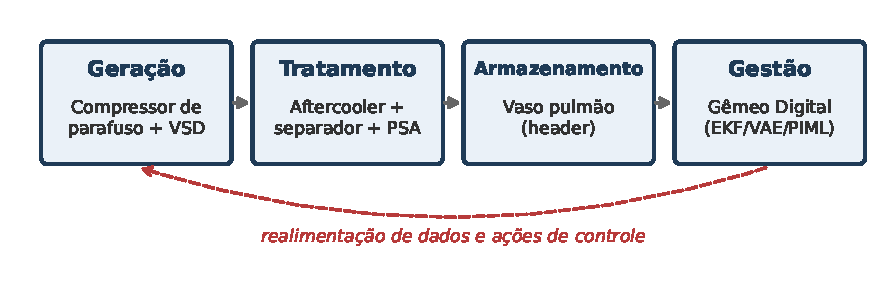
\includegraphics[width=0.75\textwidth]{figuras/fig_2_2_arquitetura.pdf}
		\caption[Diagrama de blocos da arquitetura do sistema]{Diagrama de blocos da arquitetura do sistema: os quatro pilares funcionais e a realimentação do Gêmeo Digital sobre a planta física.}
		\label{fig:2-1}
	\end{figure}

	\subsection{\textbf{Princípio de Funcionamento do Compressor de Parafuso}}
	Antes de qualquer equacionamento, é necessário compreender o princípio físico que gera a compressão: dois rotores helicoidais — o macho, com lóbulos convexos, e a fêmea, com cavidades côncavas — giram engrenados dentro de uma carcaça cilíndrica dupla \cite{hanlon}. A relação de lóbulos mais comum é $4{:}6$ (quatro lóbulos no macho para seis cavidades na fêmea), um perfil assimétrico desenvolvido para minimizar as áreas de vedação e o vazamento interno \cite{lysholm}. A Figura~\ref{fig:2-2} mostra o perfil real desse engrenamento assimétrico (aqui numa relação $5{:}6$, mesmo princípio geométrico) — repare como o contorno de um rotor é o negativo do outro, mantendo contato de vedação contínuo ao longo de toda a rotação.

	\begin{figure}[h!tbp]
		\centering
		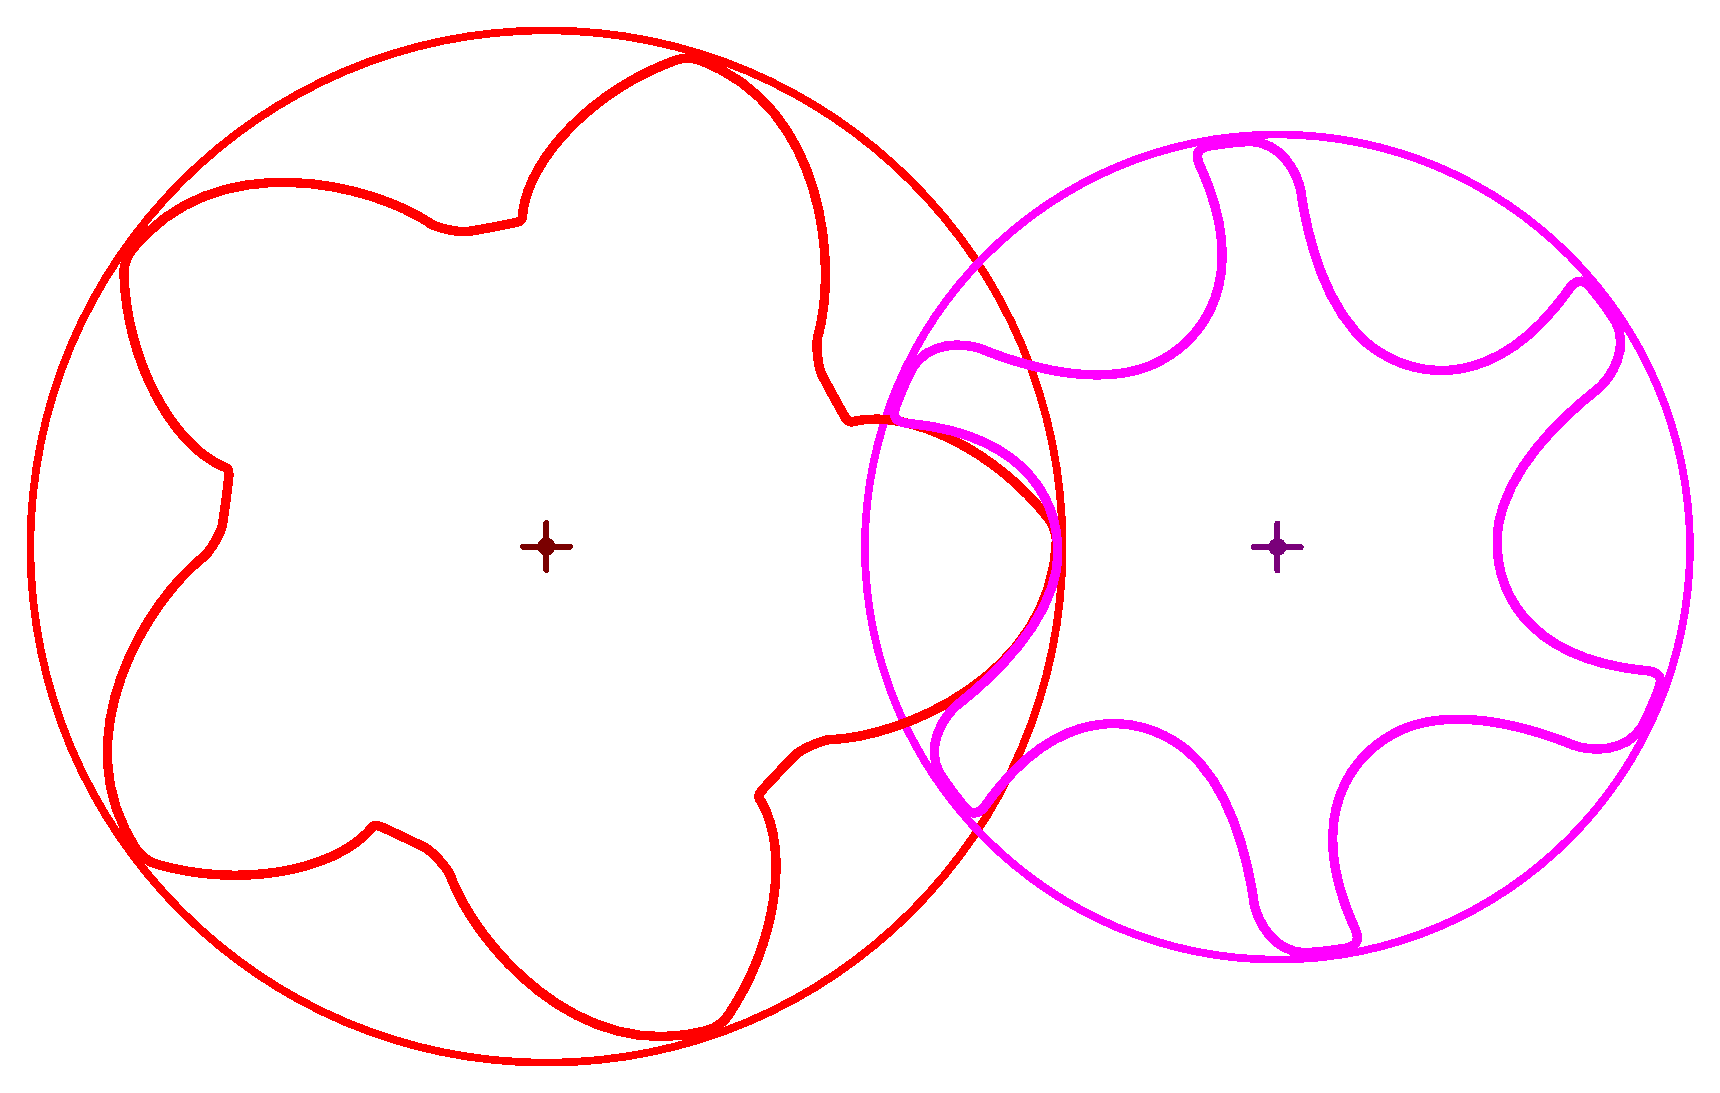
\includegraphics[width=0.60\textwidth]{figuras/fig_2_1_rotores.pdf}
		\caption[Perfil de engrenamento assimétrico de rotores helicoidais]{Perfil de engrenamento assimétrico de rotores helicoidais (relação 5:6), com centros dos eixos indicados. Adaptado de \textit{Asymmetric Screw Compressor Rotor Mesh}, Slashme, Wikimedia Commons, licença CC BY-SA 4.0 (traços reforçados e marcadores de centro adicionados pelo autor).}
		\label{fig:2-2}
	\end{figure}

	O ciclo de trabalho ocorre em três fases sequenciais, repetidas continuamente a cada engrenamento:
	\begin{enumerate}
		\item \textbf{Admissão:} À medida que os rotores giram e se desengrenam na extremidade de sucção, uma câmara em forma de ``V'' se abre entre os lóbulos e a carcaça, e o ar atmosférico preenche esse volume crescente.
		\item \textbf{Compressão:} Conforme a rotação avança, o ponto de engrenamento entre macho e fêmea se desloca ao longo do comprimento helicoidal dos rotores, fechando progressivamente a câmara e reduzindo seu volume — é essa redução puramente geométrica, sem válvulas de admissão ou descarga no sentido alternativo, que caracteriza a compressão como um processo de deslocamento positivo contínuo (ao contrário do compressor alternativo, que comprime em pulsos, ou do centrífugo, que comprime por troca de quantidade de movimento).
		\item \textbf{Descarga:} Quando a câmara em compressão alcança a aresta da porta de descarga — posição fixada pela geometria da carcaça, não por uma válvula —, o volume comprimido é liberado para a linha de descarga. É exatamente essa posição fixa da aresta de descarga que define a razão volumétrica interna $V_i$, detalhada mais adiante neste documento.
	\end{enumerate}
	Nos compressores do escopo deste documento (isentos de óleo), não há filme de óleo na câmara de trabalho para transmitir torque de um rotor ao outro por contato direto; por isso os dois eixos são sincronizados externamente por um par de engrenagens de precisão (\textit{timing gears}), mantendo uma folga constante e sem contato metal-metal entre os lóbulos durante toda a rotação — mecanismo cuja dinâmica é modelada em capítulo posterior.

	\subsection{\textbf{Cadeia de Geração e Compressão}}
	A unidade central é o compressor de parafuso rotativo, classificado como uma máquina de deslocamento positivo.
	\begin{itemize}
		\item \textbf{Rotores Helicoidais:} O par de rotores (macho e fêmea) reduz o volume do ar admitido através do engrenamento contínuo.
		\item \textbf{Motor Elétrico e VSD:} O acionamento é realizado por um motor de indução trifásico. O inversor de frequência (\textit{Variable Speed Drive} - VSD) modula a velocidade angular $\omega$ para parear a vazão produzida com a demanda da planta, operando na faixa de pressão de $7\,\text{bar}$ a $10\,\text{bar}$.
	\end{itemize}

	Para visualizar como esses elementos se conectam fisicamente — do acionamento elétrico até a descarga final de alta pressão —, a Figura~\ref{fig:2-3} apresenta o trem de compressão completo em perspectiva 3D: o motor elétrico aciona a caixa multiplicadora (gearbox) através de um acoplamento flexível; a gearbox distribui a rotação para os dois estágios de compressão (pinhões LP e HP engrenados à coroa central, mesma cinemática detalhada no Capítulo de Engenharia do Trem de Transmissão); o ar atmosférico admitido no estágio de baixa pressão (LP) é resfriado no intercooler antes de seguir para o estágio de alta pressão (HP), de onde é descarregado para o tratamento posterior (aftercooler e secagem, detalhados nos capítulos seguintes). É um esquema ilustrativo, não um desenho de projeto: motor, gearbox e tubulação são representados por formas geométricas simples, enquanto os dois pares de rotores reaproveitam a mesma técnica de varredura helicoidal usada no render do elemento compressor isolado apresentado no capítulo seguinte, em escalas proporcionalmente diferentes entre os estágios LP e HP (o de menor pressão é fisicamente maior, o de maior pressão é mais compacto).

	\begin{figure}[h!tbp]
		\centering
		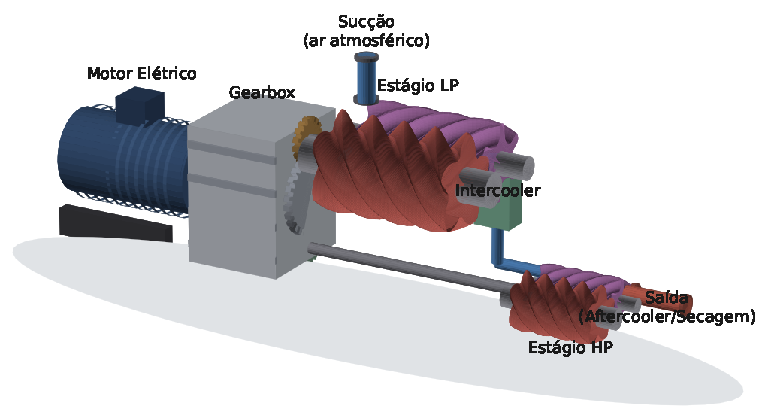
\includegraphics[width=0.80\textwidth]{figuras/fig_2_3_conjunto3d.pdf}
		\caption[Trem de compressão completo em perspectiva 3D]{Trem de compressão completo em perspectiva 3D — do motor elétrico ao estágio HP e à saída para tratamento, passando pela gearbox e pelo intercooler. Esquema ilustrativo; motor, gearbox e tubulação são formas 3D simplificadas, e os pares de rotores reaproveitam a varredura helicoidal do perfil de engrenamento adaptado de \textit{Asymmetric Screw Compressor Rotor Mesh}, Slashme, Wikimedia Commons, licença CC BY-SA 4.0.}
		\label{fig:2-3}
	\end{figure}

	\subsection{\textbf{Subsistema de Resfriamento e Separação}}
	Devido ao processo de compressão ser aproximadamente adiabático, a temperatura do ar na descarga do elemento compressor é elevada.
	\begin{itemize}
		\item \textbf{Aftercooler (Resfriador Posterior):} Trocador de calor que utiliza água do mar ou ar ambiente para reduzir a temperatura do ar comprimido.
		\item \textbf{Separador de Condensado:} Dispositivo que remove a água líquida precipitada após o resfriamento.
	\end{itemize}

	\subsection{\textbf{Invólucro do Pacote (Hood) e Ventilação Forçada}}
	Além do calor rejeitado pelo próprio ar comprimido nos trocadores de processo, o pacote compressor dissipa uma quantidade significativa de calor \textbf{para dentro do seu próprio invólucro} (\textit{hood}/\textit{canopy} acústico): perdas do motor elétrico, do VSD, da caixa multiplicadora e a própria superfície quente do elemento compressor e da tubulação interna aquecem o ar confinado dentro do gabinete. Um exaustor força a saída desse ar quente e a entrada de ar ambiente renovado, evitando que a temperatura interna do invólucro comprometa a eletrônica de potência e o isolamento do motor.
	\begin{itemize}
		\item \textbf{Fontes de Calor Internas ao Invólucro ($\dot{Q}_{\text{gerado}}$):} A soma das perdas térmicas de todos os componentes que dissipam calor para dentro do gabinete, já modeladas individualmente nos capítulos anteriores — perdas do motor, do VSD (Equação~\eqref{eq:s4-3}), da gearbox (Equação~\eqref{eq:s5-2}) e a convecção/radiação da carcaça quente do elemento compressor ($\dot{Q}_{\text{casco}}$), conforme a Equação~\eqref{eq:s2-1}:
		\begin{equation}\label{eq:s2-1}
\dot{Q}_{\text{gerado}} = \dot{W}_{\text{mot}}(1 - \eta_{\text{mot}}) + P_{\text{loss,VSD}} + P_{\text{loss,gb}} + \dot{Q}_{\text{casco}}
\end{equation}
		\item \textbf{Capacidade de Remoção do Exaustor ($\dot{Q}_{\text{hood}}$):} A Equação~\eqref{eq:s2-2} calcula quanto calor o exaustor efetivamente remove, em função da vazão mássica de ar de ventilação forçada pelo exaustor ($\dot{m}_{\text{vent}}$) e do aumento de temperatura entre a admissão de ar renovado e a exaustão do ar quente:
		\begin{equation}\label{eq:s2-2}
\dot{Q}_{\text{hood}} = \dot{m}_{\text{vent}} \cdot c_p \cdot (T_{\text{exaustão}} - T_{\text{amb}})
\end{equation}
		Em regime permanente, o invólucro só mantém temperatura interna estável se $\dot{Q}_{\text{hood}} \ge \dot{Q}_{\text{gerado}}$; a folga entre os dois lados dessa desigualdade é a margem de projeto da ventilação forçada.
		\item \textbf{Mecanismo de Falha:} Obstrução do filtro de admissão do exaustor, pá do ventilador danificada, motor do exaustor em falha, ou obstrução das venezianas de exaustão por sujeira/sal — qualquer um reduz $\dot{m}_{\text{vent}}$ e desequilibra a Equação~\eqref{eq:s2-2}.
		\item \textbf{Detecção:} Aumento progressivo de $T_{\text{exaustão}}$ para a mesma carga térmica interna estimada é o indicador primário; o Gêmeo Digital deve correlacionar esse aumento com o fator de desclassificação (\textit{derating}) do VSD (Capítulo de Subsistema Elétrico) e com a degradação acelerada do isolamento do motor pela Equação de Arrhenius (Equação~\eqref{eq:s4-7}) — ambos amplificados por uma falha silenciosa de ventilação do invólucro.
		\item \textbf{Função Acústica do Invólucro:} O mesmo gabinete modelado termicamente acima cumpre, simultaneamente, o papel de barreira de ruído — daí o qualificativo \textit{canopy acústico} usado desde a abertura desta seção. O nível de pressão sonora garantido do pacote é medido e declarado segundo a ISO 2151 \cite{iso2151}, código de ensaio específico para compressores e bombas de vácuo (a própria ISO 1217, já citada no Capítulo 1 para o FAD, exclui explicitamente ensaios de ruído do seu escopo e remete a essa norma). O limite típico de exposição ocupacional a bordo é o que dimensiona a atenuação exigida do invólucro — um requisito independente da ventilação forçada, e por vezes conflitante com ela: mais área de abertura para vazão de ar de resfriamento tende a reduzir a atenuação acústica, de modo que o projeto do exaustor não pode ser otimizado isoladamente do requisito de ruído.
	\end{itemize}

	\subsection{\textbf{Tratamento de Ar (Secagem e Filtragem)}}
	Para atender aos padrões de ar de instrumentação, o fluido deve passar por um processo de purificação rigoroso.
	\begin{itemize}
		\item \textbf{Secadora PSA (\textit{Pressure Swing Adsorption}):} Composta por duas torres preenchidas com material dessecante. Enquanto uma torre adsorve a umidade sob alta pressão, a outra regenera-se através da expansão de uma parte do ar seco (purga).
		\item \textbf{Trens de Filtragem:} Filtros coalescentes e de partículas que removem aerossóis de óleo e contaminantes sólidos.
	\end{itemize}
	
	\subsection{\textbf{Vaso de Pressão (Pulmão de Armazenamento)}}
	O reservatório de ar comprimido atua como um amortecedor de pulsações e um buffer de energia.
	\begin{itemize}
		\item \textbf{Função Estabilizadora:} Compensa picos de demanda sem causar quedas bruscas na pressão de linha.
		\item \textbf{Cálculo de Capacidade:} O volume do vaso $V_{\text{res}}$ é dimensionado com base na variação de pressão permitida $\Delta P$, pela Equação~\eqref{eq:s2-3}:
		\begin{equation}\label{eq:s2-3}
 V_{\text{res}} = \frac{t \cdot (\dot{V}_{\text{consumo}} - \dot{V}_{\text{comp}}) \cdot P_{\text{atm}}}{\Delta P} 
\end{equation}
		Onde $t$ é o tempo de autonomia desejado (intervalo em que o vaso deve sustentar sozinho o déficit entre consumo e produção antes que $\Delta P$ seja excedido).
	\end{itemize}
	
	\subsection{\textbf{Gestor de Pressão e Monitoramento de Consumo}}
	A gestão do sistema é realizada por um controlador lógico que atua como a interface primária para o Gêmeo Digital.
	\begin{itemize}
		\item \textbf{Transdutores de Pressão:} Instalados em pontos estratégicos para monitorar perdas de carga ($\Delta P_{\text{filtros}}$).
		\item \textbf{Medidores de Vazão:} Sensores que quantificam o consumo real da plataforma.
		\item \textbf{Lógica de Controle:} Mantém a pressão de rede em um valor de ajuste (\textit{setpoint}) ajustando a rampa do VSD.
	\end{itemize}

	\subsection{\textbf{Fechamento Térmico do Invólucro}}
	As Equações~\eqref{eq:s2-1} e~\eqref{eq:s2-2} definem, respectivamente, a carga térmica gerada dentro do invólucro e a capacidade do exaustor de removê-la, mas nenhuma das duas fecha qual temperatura de regime permanente o ar confinado atinge — a mesma lacuna que o Capítulo 9 tinha para a carcaça do estágio LP antes de ser fechada. O caminho de ventilação forçada tem uma \textbf{entrada}, de ar externo renovado admitido pelo exaustor à temperatura ambiente $T_{amb}$, e uma \textbf{saída}, do mesmo ar já aquecido pela carga térmica interna e descarregado à temperatura $T_{\text{exaustão}}$ — as duas pontas já presentes na própria Equação~\eqref{eq:s2-2}. Assumindo mistura completa do ar confinado (o ar de exaustão representa a própria temperatura interna do invólucro, $T_{\text{hood}} \equiv T_{\text{exaustão}}$) e substituindo a Equação~\eqref{eq:s2-1} na~\eqref{eq:s2-2} em regime permanente ($\dot Q_{\text{hood}} = \dot Q_{\text{gerado}}$, a condição de estabilidade já discutida ali), chega-se à Equação~\eqref{eq:s2-4}:
	\begin{equation}\label{eq:s2-4}
 T_{\text{hood}} = T_{amb} + \frac{\dot{Q}_{\text{gerado}}}{\dot{m}_{\text{vent}} \cdot c_p}
\end{equation}
	Essa é a temperatura que efetivamente banha todo equipamento confinado no mesmo invólucro — motor, VSD, gearbox e a carcaça do elemento compressor —, não $T_{amb}$ externo. Isso importa diretamente para o fechamento do balanço térmico da carcaça feito no Capítulo 9 (Equações~\eqref{eq:s9-14}--\eqref{eq:s9-17}): aquelas equações usam $T_{amb}$ como referência de convecção, o que é correto apenas para uma instalação a céu aberto, sem invólucro. No arranjo mais comum em plantas offshore por restrição de ruído — motor, gearbox e os dois estágios de compressão dentro do mesmo \textit{canopy} acústico, como descrito na abertura desta seção —, a referência correta nas Equações~\eqref{eq:s9-15}--\eqref{eq:s9-17} é $T_{\text{hood}}$ da Equação~\eqref{eq:s2-4}, não a temperatura ambiente externa.

	Isso também resolve uma aparente circularidade entre os dois capítulos: o termo $\dot{Q}_{\text{casco}}$ da Equação~\eqref{eq:s2-1} é a mesma grandeza física que o Capítulo 9 soma como $\dot{Q}_{\text{ext}} + \dot{Q}_{\text{arref}}$ — o calor que a carcaça entrega ao ar do invólucro por convecção (natural mais forçada). Em regime permanente esse total iguala $\dot{Q}_{\text{int}}$ (Equação~\eqref{eq:s9-14}, pela própria Equação~\eqref{eq:s9-6}), de modo que $\dot{Q}_{\text{casco}} = \dot{Q}_{\text{int}}$ pode ser calculado diretamente a partir da perda mecânica do estágio LP, sem exigir $T_c$ como entrada. A ordem de cálculo correta é, portanto, sequencial e não simultânea: (1) $\dot{Q}_{\text{int}}$ pela Equação~\eqref{eq:s9-14}, a partir do ponto de operação; (2) $\dot{Q}_{\text{gerado}}$ (Equação~\eqref{eq:s2-1}, usando $\dot{Q}_{\text{casco}}=\dot{Q}_{\text{int}}$) e $T_{\text{hood}}$ (Equação~\eqref{eq:s2-4}); (3) $T_c$ (Equação~\eqref{eq:s9-16}, agora referenciada a $T_{\text{hood}}$). Para instalações sem invólucro — compressor a céu aberto —, esta subseção inteira não se aplica: a carcaça convecciona diretamente para $T_{amb}$, como nas Equações~\eqref{eq:s9-15}--\eqref{eq:s9-17} originais.

	\vspace{1em}
	\hrule
	\vspace{1em}

	\textbf{Diretriz Técnica Final:} A arquitetura descrita aqui — geração por parafuso isento de óleo, tratamento por resfriamento/secagem e armazenamento em vaso pulmão — define os quatro blocos físicos que o Gêmeo Digital deve modelar de forma acoplada; tratar qualquer um isoladamente (por exemplo, otimizar o compressor sem considerar o impacto na secadora a jusante) produz um modelo incompleto e recomendações potencialmente contraditórias. A Equação~\eqref{eq:s2-4} acrescenta uma consequência prática direta para instalações com invólucro acústico: qualquer equação térmica de um componente interno (Equação~\eqref{eq:s9-6} da carcaça, entre outras) só está correta se referenciada a $T_{\text{hood}}$, não à ambiente externa — usar $T_{amb}$ nesse contexto subestima sistematicamente a temperatura real de operação.

	% --- Fim do Capítulo 2 ---
	
	% --- Início do Capítulo 3 ---
	
	\clearpage
	\section{\textbf{Detalhamento de Componentes, Acessórios e Instrumentação}}
	
	Antes de detalhar cada subsistema individualmente, é útil visualizar o coração do pacote: o elemento compressor (\textit{airend}), onde os dois rotores helicoidais executam fisicamente a compressão. A Figura~\ref{fig:3-1} apresenta o par de rotores em perspectiva tridimensional, obtida por varredura helicoidal do mesmo perfil de engrenamento assimétrico $5{:}6$ já apresentado na Figura~\ref{fig:2-2}: o rotor macho (à direita) recebe uma torção total de $300^\circ$ ao longo do comprimento, enquanto a fêmea gira em sentido contrário com hélice oposta, na razão $5/6$ da torção do macho — exatamente a relação cinemática que mantém o contato de vedação contínuo durante a rotação. Os tocos de eixo nas extremidades são os assentos dos rolamentos e, no lado de acionamento, a interface com a caixa multiplicadora (\textit{gearbox}). As subseções seguintes detalham os blocos que cercam esse núcleo — motor elétrico, acoplamento, gearbox e acessórios — e sua instrumentação associada, seguindo a mesma organização por subsistema já consolidada na literatura de referência sobre tecnologia de compressores \cite{bloch}.

	\begin{figure}[h!tbp]
		\centering
		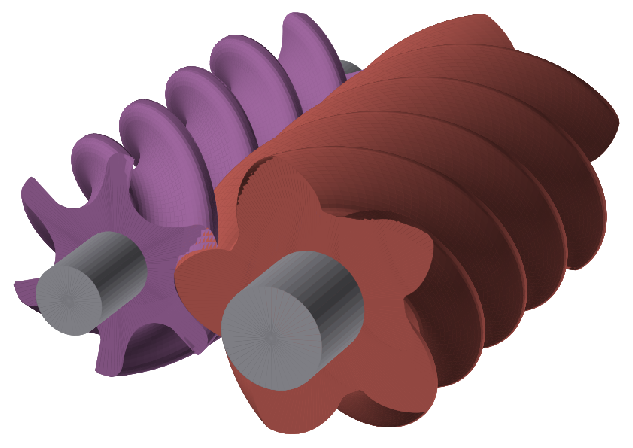
\includegraphics[width=0.80\textwidth]{figuras/fig_3_1_parafuso3d.pdf}
		\caption[Par de rotores helicoidais do elemento compressor (3D)]{Par de rotores helicoidais do elemento compressor (\textit{airend}) em perspectiva 3D, gerado por varredura helicoidal do perfil de engrenamento da Figura~\ref{fig:2-2} (torção de $300^\circ$ no rotor macho, relação $5{:}6$, hélices opostas). Elaboração 3D original do autor; perfil 2D adaptado de \textit{Asymmetric Screw Compressor Rotor Mesh}, Slashme, Wikimedia Commons, licença CC BY-SA 4.0.}
		\label{fig:3-1}
	\end{figure}

	\subsection{\textbf{Subsistema de Potência e Acionamento}}
	\begin{itemize}
		\item \textbf{Painel Elétrico e VSD:} O painel elétrico é o ponto de entrega de energia do pacote — recebe a alimentação de média/baixa tensão da plataforma, protege o circuito com relés de disparo (detalhados no Capítulo de Subsistema Elétrico) e abriga o Inversor de Frequência (\textit{Variable Speed Drive}, VSD). O VSD converte a frequência fixa da rede numa frequência variável, permitindo modular a velocidade angular $\omega$ do motor para casar a vazão produzida com a demanda da planta em vez de operar sempre a rotação nominal. O efeito colateral desse chaveamento eletrônico de alta frequência é a distorção harmônica total de corrente ($\text{THD}_i$) injetada na rede — quanto maior a distorção, maior o aquecimento adicional no motor e a interferência em outros equipamentos sensíveis da rede elétrica isolada da plataforma, por isso ela é monitorada e mitigada (filtros de linha, técnicas de modulação PWM).
		\item \textbf{Motor Elétrico:} Motor de indução trifásico responsável por converter a energia elétrica recebida do VSD em energia mecânica no eixo, entregue ao trem de potência (Capítulo de Trem de Potência). A eficiência de conversão $\eta_{\text{mot}}$ é a razão entre a potência mecânica efetivamente disponível no eixo e a potência elétrica consumida — a diferença entre as duas é dissipada como calor nos enrolamentos e no núcleo, e é justamente essa parcela de perda que aquece o motor e limita sua vida útil. O circuito equivalente completo, o escorregamento e os mecanismos de falha elétrica (incluindo desbalanço entre fases) são modelados em detalhe no Capítulo de Subsistema Elétrico.
	\end{itemize}
	
	\subsection{\textbf{Unidade Compressora e Circuito de Óleo}}
	\begin{itemize}
		\item \textbf{Elemento Compressor:} É o próprio par de rotores helicoidais (\textit{airend}) apresentado na Figura~\ref{fig:3-1} — o núcleo físico onde a compressão de fato acontece, por redução geométrica contínua do volume entre os lóbulos em engrenamento (ciclo já descrito no Capítulo de Arquitetura). A vazão mássica teórica que ele entrega, Equação~\eqref{eq:s3-1}, é o produto da densidade do ar de sucção pelo volume deslocado pelo par de rotores a cada rotação completa ($V_{\text{disp}}$, fixado pela geometria do perfil helicoidal — comprimento, diâmetro e ângulo de hélice dos rotores) e pela rotação, corrigido pela eficiência volumétrica real $\eta_{\text{vol}}$:
		\begin{equation}\label{eq:s3-1}
 \dot{m} = \rho \cdot V_{\text{disp}} \cdot \frac{\omega}{2\pi} \cdot \eta_{\text{vol}}
\end{equation}
		O termo $\eta_{\text{vol}}$ é o que separa a vazão teórica (puramente geométrica) da vazão real: parte do ar comprimido escapa de volta para câmaras de pressão mais baixa através das folgas microscópicas entre rotores e carcaça, um mecanismo detalhado no Capítulo de Termodinâmica do Estágio LP. Quanto maior o desgaste dessas folgas ao longo da vida do equipamento, menor $\eta_{\text{vol}}$ e maior o desvio entre a vazão prevista por esta equação e a vazão real entregue à rede.
		\item \textbf{Separador de Ar/Óleo (Deaeração do Circuito de Lubrificação):} Como o compressor deste documento é isento de óleo na câmara de compressão (não há óleo em contato com o ar de processo), este separador não atua no ar comprimido em si, mas no óleo de lubrificação da gearbox e dos mancais: o óleo que retorna ao cárter após lubrificar engrenagens e mancais chega aerado (com bolhas de ar incorporadas pelo respingo/turbulência do engrenamento), e precisa liberar esse ar antes de ser recirculado pela bomba — óleo aerado perde capacidade de sustentar o filme lubrificante e de dissipar calor. A perda de carga que esse separador impõe ao próprio óleo, $\Delta P_{\text{sep}}$, é monitorada porque seu aumento progressivo indica saturação ou obstrução do elemento.
	\end{itemize}
	
	\subsection{\textbf{Resfriamento e Drenagem}}
	\begin{itemize}
		\item \textbf{Resfriador final (\textit{aftercooler}):} É o trocador de calor final do pacote, posicionado logo após a descarga do último estágio de compressão (HP) e antes da filtragem/secagem. Sua função é reduzir a temperatura do ar — tipicamente acima de $100\,^{\circ}\text{C}$ na saída do estágio HP — para um patamar compatível com os elementos filtrantes e, principalmente, para forçar a condensação da umidade que o ar carrega antes que ela chegue ao secador PSA (detalhado no Capítulo de Secagem). Normalmente é resfriado a água do mar ou a ar ambiente, conforme a disponibilidade na plataforma. Sua taxa de rejeição térmica, Equação~\eqref{eq:s3-2}, segue a forma clássica de projeto de trocadores — coeficiente global de transferência ($U$, que piora com incrustação/\textit{fouling}) vezes área de troca ($A$, fixa por projeto) vezes a diferença de temperatura média logarítmica ($\Delta T_{\text{LMTD}}$, detalhada no Capítulo de Dinâmica do Intercooler):
		\begin{equation}\label{eq:s3-2}
 \dot{Q} = U \cdot A \cdot \Delta T_{\text{LMTD}}
\end{equation}
		Como $A$ é fixa, qualquer queda na taxa de calor removido para a mesma vazão e mesma diferença de temperatura de entrada só pode ser explicada por uma queda em $U$ — é esse raciocínio que permite ao Gêmeo Digital atribuir uma perda de performance térmica à incrustação do trocador, e não a outra causa.
		\item \textbf{Drenos Automáticos:} Válvulas que removem periodicamente a água líquida que se acumula no fundo do vaso separador de condensado, logo após o aftercooler — o mesmo condensado quantificado no Capítulo de Intercooler. Podem ser acionadas por um sensor de nível (abrem só quando há líquido acumulado, mais eficiente) ou por temporizador (abrem em ciclos fixos, mais simples porém desperdiça ar comprimido a cada purga). Um dreno que trava aberto perde ar de processo continuamente; um que trava fechado permite que a água se acumule e seja arrastada para os estágios seguintes — ambos os modos de falha são detalhados no Capítulo de Aftercooler e Filtragem.
	\end{itemize}
	
	\subsection{\textbf{Purificação e Secagem (Sistema PSA)}}
	\begin{itemize}
		\item \textbf{Torres de Adsorção:} Duas colunas cilíndricas preenchidas com material dessecante (tipicamente \textbf{Alumina Ativada} ou peneira molecular) que retém fisicamente as moléculas de vapor d'água na superfície de seus grãos porosos à medida que o ar úmido passa por elas sob pressão. O princípio de adsorção por oscilação de pressão (\textit{Pressure Swing Adsorption}, PSA) alterna as duas torres entre dois papéis: enquanto uma seca o ar de processo, a outra é regenerada — o ciclo completo, a cinética de saturação do leito e o cálculo do ponto de orvalho resultante são detalhados no Capítulo de Sistema de Secagem.
		\item \textbf{Resistências de Aquecimento:} Utilizadas nos ciclos de regeneração térmica dos secadores que precisam de calor externo para ``expulsar'' a umidade retida no dessecante saturado (ao contrário dos secadores PSA a frio, que regeneram apenas por expansão do ar de purga). A Equação~\eqref{eq:s3-3} calcula a potência elétrica necessária como a vazão mássica de ar de purga vezes o calor específico do ar vezes o salto de temperatura imposto a esse ar de regeneração:
		\begin{equation}\label{eq:s3-3}
 P_{\text{term}} = \dot{m}_{\text{purge}} \cdot c_p \cdot \Delta T
\end{equation}
		Esse consumo elétrico de regeneração é significativo o suficiente para justificar a recuperação de calor residual de outras partes do pacote (aftercooler, óleo, exaustão do invólucro), estratégia detalhada no Capítulo de Sistema de Secagem.
		\item \textbf{Válvulas de Comutação:} Válvulas solenoides que alternam o caminho do fluxo de ar entre as duas torres a cada ciclo — direcionando o ar úmido de processo para a torre em adsorção e o ar de purga (ou o ar quente de regeneração) para a torre que está sendo regenerada. Uma falha de comutação (válvula presa ou com vazamento entre torres) compromete a secagem mesmo com o leito dessecante em boas condições, por isso é diagnosticada separadamente da saturação do próprio material.
	\end{itemize}
	
	\subsection{\textbf{Filtragem e Válvulas de Linha}}
	\begin{itemize}
		\item \textbf{Filtros Coalescentes:} Elementos filtrantes de meio fibroso instalados a jusante do aftercooler que capturam aerossóis finos de óleo (do circuito de lubrificação) e partículas sólidas residuais, protegendo o leito dessecante do secador PSA — o material adsorvente é facilmente contaminado e perde capacidade permanentemente se exposto a óleo. À medida que o meio filtrante retém contaminantes, a perda de carga que ele impõe ao escoamento cresce; a Equação~\eqref{eq:s3-4} modela essa perda pela forma clássica de perda de carga localizada — coeficiente de perda do elemento filtrante ($\zeta$, que cresce com a saturação) vezes a pressão dinâmica do escoamento:
		\begin{equation}\label{eq:s3-4}
 \Delta P = \zeta \cdot \frac{\rho v^2}{2}
\end{equation}
		Como $\rho$ e $v$ variam com a condição de operação, o Gêmeo Digital normaliza $\Delta P$ medido por essas duas variáveis antes de comparar contra o limite de substituição do elemento — comparar $\Delta P$ bruto entre duas condições de carga distintas levaria a falsos alarmes.
		\item \textbf{Válvulas de Bloqueio e Retenção:} Duas famílias com papéis distintos: as válvulas de \textbf{bloqueio} (manuais ou motorizadas) isolam trechos da tubulação para manutenção sem despressurizar todo o sistema; as válvulas de \textbf{retenção} (\textit{check valves}) permitem o fluxo em um único sentido e impedem que o ar armazenado no vaso pulmão reflua para o compressor quando este for parado ou perder pressão — sem elas, a parada de uma unidade em operação em frota (Capítulo de Distribuição e Armazenamento) despressurizaria seu próprio circuito através da rede comum.
	\end{itemize}
	
	\subsection{\textbf{Armazenamento e Segurança}}
	\begin{itemize}
		\item \textbf{Vaso de Pressão (Pulmão):} Reservatório cilíndrico de ar já seco e filtrado, dimensionado conforme ASME Seção VIII Div. 1 para operar até aproximadamente $10\,\text{bar}$. Funciona como um amortecedor de pulsações e um buffer de energia entre a produção (descontínua, sujeita a ciclos de carga/alívio do compressor) e o consumo da planta — sem ele, cada oscilação de demanda se propagaria diretamente para a pressão de rede. Sua dinâmica de pressão interna, Equação~\eqref{eq:s3-5}, é proporcional ao desbalanço instantâneo entre a vazão que entra (produção) e a que sai (consumo da planta):
		\begin{equation}\label{eq:s3-5}
 \frac{dP_{\text{res}}}{dt} = \frac{R T}{V} \Delta \dot{m}
\end{equation}
		Quando $\Delta \dot{m} = 0$ (produção e consumo equilibrados), a pressão do vaso permanece constante; um $\Delta \dot{m}$ persistentemente negativo (consumo maior que produção) é o sinal precoce de que a rede está prestes a atingir um nível de alarme de pressão baixa (Capítulo de Distribuição e Armazenamento).
		\item \textbf{PSV (Válvula de Segurança):} \textit{Pressure Safety Valve} — dispositivo puramente mecânico, independente de qualquer lógica de controle ou instrumentação eletrônica, que abre automaticamente por ação de mola quando a pressão interna excede um limite pré-ajustado, aliviando o excesso para a atmosfera. É a última camada de proteção contra sobrepressão do vaso, exigida pela norma ASME VIII como redundância física ao controle de pressão normal do sistema — mesmo que toda a lógica de controle do Gêmeo Digital falhe, a PSV continua protegendo o equipamento. \textbf{Nota de escopo:} o dimensionamento do orifício de alívio (área mínima de passagem exigida pela ASME VIII Div. 1 \cite{asme8} para a condição de sobrepressão de projeto) é matéria de projeto do vaso, resolvida uma única vez na especificação do equipamento — não uma grandeza que o Gêmeo Digital calcula ou monitora em operação. O papel do modelo aqui se limita a detectar os dois modos de falha operacional da PSV já instrumentada (travada aberta ou fechada), não a substituir o cálculo de dimensionamento.
	\end{itemize}
	
	\subsection{\textbf{Instrumentação}}
	\begin{itemize}
		\item \textbf{Transdutores e Sensores:} O conjunto de pontos de medição distribuídos ao longo de todo o trem descrito neste capítulo — pressão ($P$) em cada estágio e no vaso pulmão, temperatura ($T$) na descarga de cada trocador, umidade relativa ($\phi$) e ponto de orvalho sob pressão ($T_{dp}$) na saída do secador. Nenhuma das equações apresentadas neste capítulo é calculável pelo Gêmeo Digital sem que a variável correspondente esteja de fato instrumentada em campo — é por isso que a Diretriz Técnica Final abaixo trata a cobertura de instrumentação como um limite físico do modelo, não um detalhe de implementação.
	\end{itemize}

	\vspace{1em}
	\hrule
	\vspace{1em}

	\textbf{Diretriz Técnica Final:} Cada componente listado neste capítulo é, ao mesmo tempo, um ponto físico de instrumentação e uma entrada do modelo matemático desenvolvido nos capítulos seguintes — a qualidade do Gêmeo Digital é limitada pela cobertura e pela taxa de amostragem desses sensores, não apenas pela sofisticação do equacionamento.

	% --- Fim do Capítulo 3 ---
	
	% --- Início do Capítulo 4: Subsistema Elétrico e Acionamento Dinâmico ---
	
	\clearpage
	\section{\textbf{Subsistema Elétrico e Acionamento Dinâmico}}
	
	Este capítulo detalha a modelagem do fluxo de energia desde o painel de distribuição até o eixo do compressor, integrando eletrônica de potência, eletromagnetismo e a modelagem matemática de modos de falha para o Gêmeo Digital.
	
	\subsection{\textbf{Painel Elétrico e Lógica de Proteção (Relés)}}
	O painel elétrico offshore atua como a interface de segurança primária. Os relés de proteção digitais monitoram a integridade do sistema através de curvas de tempo inverso, que devem ser replicadas no Gêmeo Digital para prever disparos (\textit{trips}) indesejados.
	
	\begin{itemize}
		\item \textbf{Equacionamento de Disparo (Norma IEC 60255 \cite{iec60255}):}
		O tempo de atuação $t_{\text{trip}}$ é modelado pela Equação~\eqref{eq:s4-1} para detectar sobrecargas térmicas antes que ocorram danos permanentes:
		\begin{equation}\label{eq:s4-1}
 t_{\text{trip}} = \frac{k_{\text{relé}} \cdot \beta_{\text{relé}}}{\left( \frac{I}{I_s} \right)^{\alpha_{\text{relé}}} - 1}
\end{equation}
		Onde:
		\begin{itemize}
			\item $I$: Corrente de carga medida em tempo real.
			\item $I_s$: Corrente de ajuste (setpoint).
			\item $\alpha_{\text{relé}}, \beta_{\text{relé}}, k_{\text{relé}}$: Constantes que definem a curva (Normalmente Inversa, Muito Inversa ou Extremamente Inversa); todas subscritas — $k_{\text{relé}}$ para não colidir com o índice de tempo discreto $k$ usado nos capítulos de EKF/MPC/PSO, e $\alpha_{\text{relé}}$/$\beta_{\text{relé}}$ para não colidir com a taxa de falsos alarmes $\alpha$ e o peso da divergência KL $\beta$ do Capítulo 22.
		\end{itemize}
		\item \textbf{Mecanismos de Falha no Painel:} O Gêmeo Digital monitora a resistência de contato e a temperatura nos barramentos. Um aumento na temperatura $T_{\text{contato}}$ sem aumento de corrente indica oxidação ou afrouxamento mecânico por vibração.
	\end{itemize}
	
	\subsection{\textbf{Inversor de Frequência (VSD - Variable Speed Drive)}}
	O VSD é o elemento de controle que modula a velocidade angular $\omega$ do motor. Ele é modelado como um conversor de potência com perdas não lineares.
	
	\begin{itemize}
		\item \textbf{Controle V/f (Tensão/Frequência):} Para manter o fluxo magnético constante no motor e evitar a saturação do núcleo, o VSD eleva a tensão de saída ($V_{\text{out}}$) na mesma proporção em que eleva a frequência ($f_{\text{out}}$), mantendo a razão entre as duas praticamente fixa em toda a faixa de rotação — relação conhecida como Equação~\eqref{eq:s4-2}:
		\begin{equation}\label{eq:s4-2}
 \frac{V_{\text{out}}}{f_{\text{out}}} \approx \text{constante}
\end{equation}
		\item \textbf{Eficiência e Perdas Térmicas:} A potência dissipada no VSD ($P_{\text{loss,VSD}}$) é fundamental para o prognóstico de falha dos módulos IGBT. A Equação~\eqref{eq:s4-3} decompõe essa dissipação em duas parcelas de origem física distinta: $P_{\text{switching}}$, a perda toda vez que o IGBT liga/desliga (proporcional à frequência de chaveamento), e $P_{\text{conduction}}$, a perda resistiva enquanto o IGBT permanece conduzindo corrente:
		\begin{equation}\label{eq:s4-3}
 P_{\text{loss,VSD}} = P_{\text{switching}} + P_{\text{conduction}}
\end{equation}
		A eficiência instantânea é dada por $\eta_{\text{vsd}} = \frac{P_{\text{out}}}{P_{\text{in}}}$. O Gêmeo Digital utiliza a distorção harmônica total ($\text{THD}_i$) para calcular o fator de desclassificação (\textit{derating}) do motor.
	\end{itemize}
	
	\subsection{\textbf{Motor Elétrico de Indução Trifásico}}
	O motor é modelado através de seu circuito equivalente em regime permanente, permitindo a detecção de anomalias eletromagnéticas; a determinação de perdas e rendimento a partir de ensaios segue a metodologia normatizada pela IEC 60034-2-1 \cite{iec60034}. A Figura~\ref{fig:4-1} mostra o motor de indução trifásico deste trem, em perspectiva 3D, com a caixa de ligação aberta expondo os terminais das três fases ($V_{L,1}$, $V_{L,2}$, $V_{L,3}$ da Equação~\eqref{eq:s4-8}), as aletas de refrigeração, os pés de fixação e o acoplamento do lado de acionamento.

	\begin{figure}[h!tbp]
		\centering
		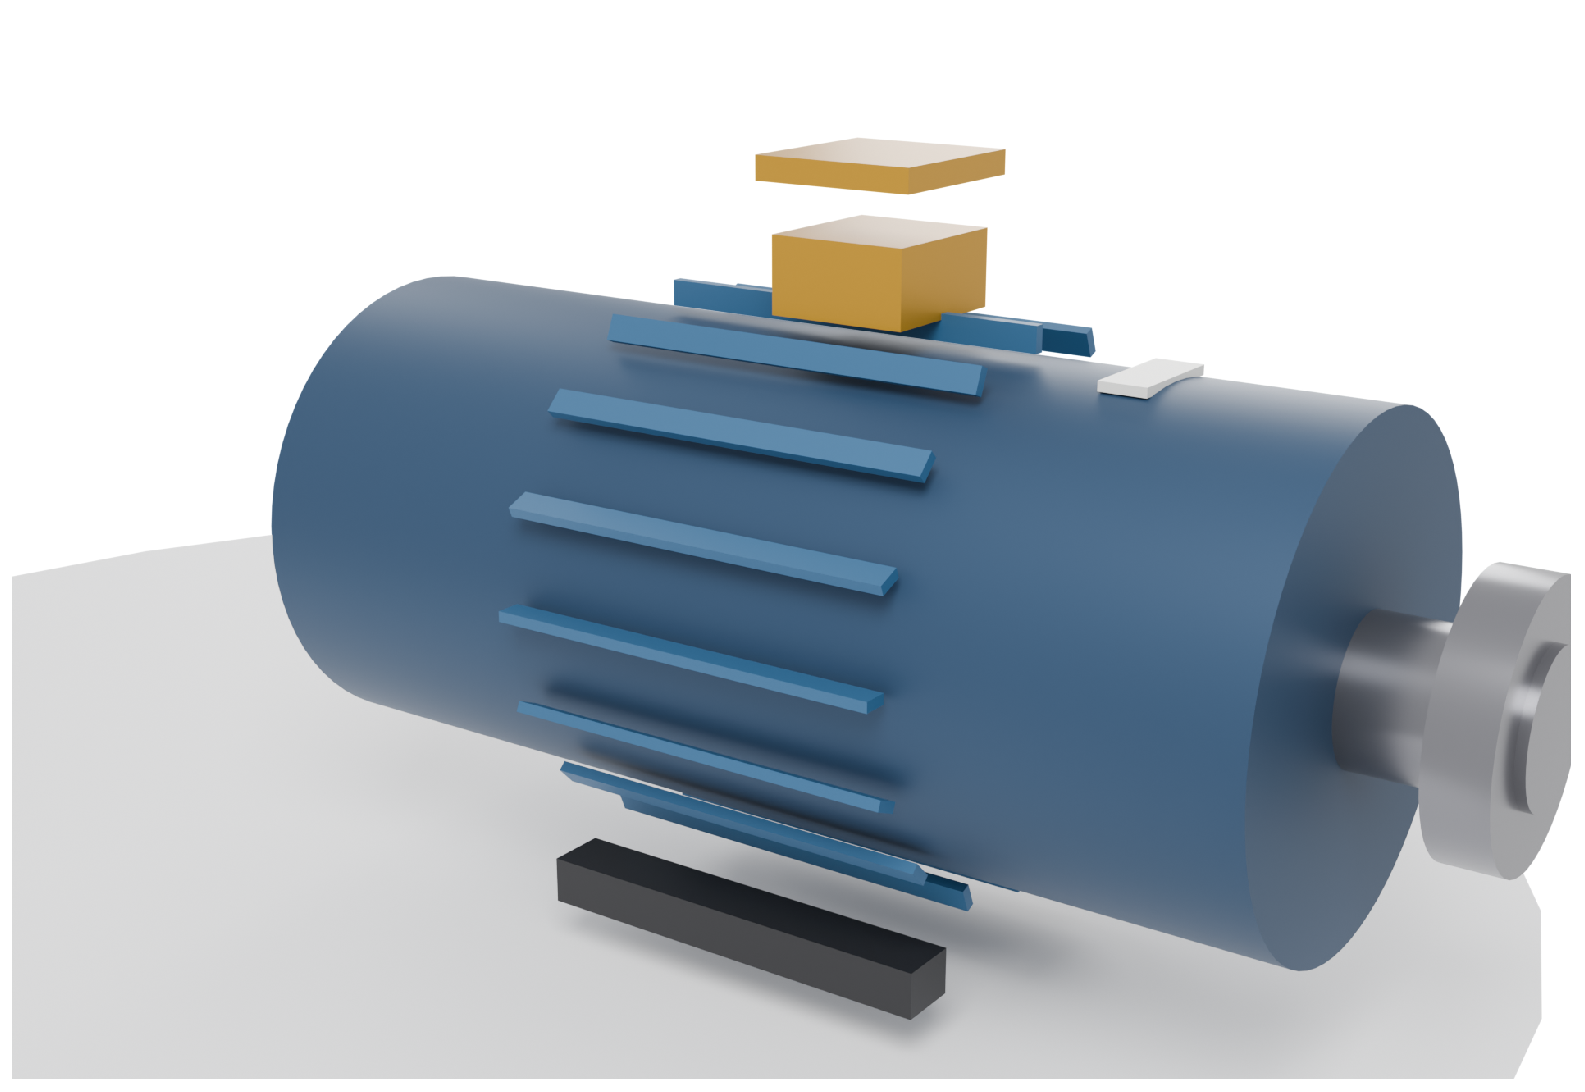
\includegraphics[width=0.70\textwidth]{figuras/fig_4_1_motor.pdf}
		\caption[Motor de indução trifásico industrial]{Motor de indução trifásico industrial, em perspectiva 3D — aletas de refrigeração, caixa de ligação das três fases, pés de fixação e acoplamento. Esquema ilustrativo, não um desenho de projeto.}
		\label{fig:4-1}
	\end{figure}

	\begin{itemize}
		\item \textbf{Cinemática e Escorregamento ($s$):}
		A rotação síncrona $n_s$ e o escorregamento $s$ são calculados pela Equação~\eqref{eq:s4-4} para determinar a carga real no compressor:
		\begin{equation}\label{eq:s4-4}
 n_s = \frac{120 \cdot f}{p} \quad \text{e} \quad s = \frac{n_s - N_{mot}}{n_s} 
\end{equation}
		Onde $p$ é o número de polos e $N_{mot}$ é a rotação medida do motor (RPM), pelo encoder ou estimada via corrente — mesma grandeza referenciada como $N_{mot}$ nos capítulos de trem de potência (não confundir com o índice politrópico $n$, usado sem subscrito nos capítulos de termodinâmica).
		\item \textbf{Torque Eletromagnético ($\tau_{em}$):}
		O torque gerado, considerando o equivalente de Thevenin do estator ($V_{th}, R_{th}, X_{th}$), é dado pela Equação~\eqref{eq:s4-5}:
		\begin{equation}\label{eq:s4-5}
 \tau_{em} = \frac{3 \cdot V_{th}^2 \cdot R_r / s}{\omega_s \cdot \left[ (R_{th} + R_r / s)^2 + (X_{th} + X_r)^2 \right]} 
\end{equation}
		Onde $R_r$ e $X_r$ são a resistência e a reatância do rotor referidas ao estator (parâmetros de placa/ensaio do motor), e $\omega_s = 2\pi n_s/60$ é a velocidade angular síncrona correspondente à rotação síncrona $n_s$ definida na Equação~\eqref{eq:s4-4}.
	\end{itemize}
	
	\subsection{\textbf{Mecanismos de Falha e Correlações para o Gêmeo Digital}}
	O diferencial do Gêmeo Digital é a capacidade de introduzir variáveis de degradação no equacionamento:
	
	\begin{enumerate}
		\item \textbf{Quebra de Barras do Rotor:} Introduz uma modulação na corrente de estator. O modelo de diagnóstico busca por bandas laterais no espectro de frequência, previstas pela Equação~\eqref{eq:s4-6}:
		\begin{equation}\label{eq:s4-6}
 f_{\text{sideband}} = f_1 (1 \pm 2js) 
\end{equation}
		Onde $f_1$ é a frequência fundamental de alimentação (rede/VSD) e $j = 1, 2, 3, \dots$ é a ordem do harmônico da banda lateral monitorada (usa-se $j$ em vez de $k$ para não colidir com a constante do relé e o índice de tempo discreto usados em outros capítulos).
		\item \textbf{Degradação do Isolamento Térmico:} Utiliza a Equação de Arrhenius, na forma da Equação~\eqref{eq:s4-7}, para estimar a vida útil residual ($L$) baseada na temperatura medida nos enrolamentos ($T_{\text{enrol}}$):
		\begin{equation}\label{eq:s4-7}
 L = L_0 \cdot \exp \left( \frac{E_a}{R_u \cdot T_{\text{enrol}}} \right)
\end{equation}
		Onde $R_u$ é a constante universal dos gases ($8{,}314\,\text{J}\,\text{mol}^{-1}\,\text{K}^{-1}$, com $E_a$ em $\text{J}\,\text{mol}^{-1}$) — subscrita para não colidir com $R$, a constante específica do ar ($287\,\text{J}\,\text{kg}^{-1}\,\text{K}^{-1}$, Nomenclatura) usada em todo o resto do documento. A degradação de isolamento elétrico é um processo de cinética química, não termofluídica: a constante do ar não tem papel físico aqui.
		\item \textbf{Excentricidade e Falhas de Rolamento:} Modeladas como um aumento no torque de atrito parasita $\tau_{\text{fric}}$, que desvia o consumo elétrico da curva teórica de compressão.
		\item \textbf{Desbalanço de Tensão/Corrente entre Fases e Sobreaquecimento Localizado:} Por ser um motor trifásico, um pequeno desbalanço entre as três tensões de linha de alimentação ($V_{L,1}, V_{L,2}, V_{L,3}$) — comum em redes elétricas isoladas offshore sujeitas a flutuações de carga (Capítulo 1) — já é suficiente para produzir um desbalanço de corrente desproporcionalmente maior entre as três fases ($I_1, I_2, I_3$), por causa da baixa impedância de sequência negativa do motor: a fase mais carregada sobreaquece localmente mesmo que a corrente de linha única ($I$, Equação~\eqref{eq:s4-1}) pareça normal. O Gêmeo Digital monitora essa condição pelos dois índices adimensionais de desbalanço, na definição padronizada pela NEMA MG1 \cite{nemamg1} — o desvio máximo de cada grandeza em relação à média das três fases, normalizado pela própria média — complementados pelo espalhamento entre as três temperaturas de enrolamento medidas por RTD dedicado por fase ($T_1, T_2, T_3$), conforme a Equação~\eqref{eq:s4-8}:
		\begin{equation}\label{eq:s4-8}
		\begin{aligned}
			VU &= 100 \cdot \frac{\max_i |V_{L,i} - \bar{V}_L|}{\bar{V}_L} \\[6pt]
			IU &= 100 \cdot \frac{\max_i |I_i - \bar{I}|}{\bar{I}} \\[6pt]
			\Delta T_{\text{fases}} &= \max(T_1, T_2, T_3) - \min(T_1, T_2, T_3)
		\end{aligned}
		\end{equation}
		Onde $\bar{V}_L$ e $\bar{I}$ são as médias das três tensões de linha e das três correntes de fase, respectivamente. Um $IU$ persistente acima de poucos pontos percentuais mesmo com $VU$ pequeno — sintoma que a corrente de linha agregada sozinha não capta — já justifica investigação de curto entre espiras ou conexão frouxa no painel.
		\item \textbf{Correntes de Eixo por Descarga Eletrostática (EDM) em Motor Acionado por VSD:} O chaveamento PWM de alta frequência do VSD (Capítulo de Subsistema Elétrico) não é eletricamente simétrico entre as três fases em cada instante de comutação, o que induz uma tensão de modo comum residual no barramento — e, por acoplamento capacitivo entre estator e rotor, uma tensão parasita no próprio eixo do motor. Quando essa tensão de eixo excede a rigidez dielétrica do filme de óleo lubrificante que separa as esferas/roletes das pistas do rolamento, o filme rompe e a energia armazenada se descarrega como um pulso de corrente — a corrente de descarga eletromagnética (EDM, \textit{Electrical Discharge Machining}) — que erode a pista a cada evento. É o mecanismo de falha elétrica mais característico de motores de alta potência com acionamento por inversor \cite{erdman}, distinto e adicional à degradação térmica do isolamento já modelada pela Equação~\eqref{eq:s4-7}: enquanto a Equação~\eqref{eq:s4-7} governa a vida do enrolamento, a EDM governa a vida do rolamento — as duas vias dominantes de mortalidade prematura de motor com VSD. A Equação~\eqref{eq:s4-13}, ao final deste capítulo, fecha essa tensão de eixo e o critério de disparo em função de parâmetros de projeto do motor, em vez de tratá-la apenas qualitativamente.
		\begin{itemize}
			\item \textbf{Indicador:} Padrão de craterização (\textit{fluting}) visível em inspeção de pista de rolamento; em campo, pico recorrente de corrente de eixo medido por sonda de corrente dedicada (\textit{shaft grounding} instrumentado), cuja progressão acompanha o histórico de operação do VSD (tempo em carga, frequência de chaveamento).
			\item \textbf{Mitigação (acessórios):} Rolamento isolado eletricamente no lado oposto ao acoplamento (\textit{Non-Drive End}), anel de aterramento de eixo (\textit{shaft grounding ring}) que oferece um caminho de descarga de baixa impedância alternativo ao rolamento, e filtro de modo comum na saída do VSD.
		\end{itemize}
		\item \textbf{Aquecedores Anticondensação (\textit{Space Heaters}):} Resistências de baixa potência instaladas no enrolamento do motor, energizadas somente com a máquina parada, cuja função é manter o enrolamento acima do ponto de orvalho do ar ambiente circundante — em atmosfera offshore salina e saturada, um motor parado e frio condensa umidade internamente a cada ciclo de resfriamento noturno, degradando o isolamento por via elétrica (trilhas de umidade, corrosão dos contatos) muito antes que a via térmica da Equação~\eqref{eq:s4-7} se torne relevante. É o acessório que protege especificamente a unidade em reserva (\textit{standby}) da frota (Capítulo 16): quanto mais tempo uma máquina permanece parada aguardando comando de partida, maior a janela de exposição à condensação, e é exatamente nesse cenário — parada prolongada em atmosfera salina saturada — que o aquecedor anticondensação atua.
	\end{enumerate}

	\subsection{\textbf{Equação de Acoplamento Global}}
	A integração final que o Gêmeo Digital resolve para o subsistema elétrico é a Equação~\eqref{eq:s4-9}:
	\begin{equation}\label{eq:s4-9}
 P_{\text{rede}} = \frac{1}{\eta_{\text{vsd}}} \left[ \frac{\tau_{\text{compressão}}(\theta, P) \cdot \omega}{\eta_{\text{mot}}(s, T)} + P_{\text{perdas\_mec}} \right]
\end{equation}
	Esta equação correlaciona a pressão de armazenamento (até $10\,\text{bar}$) com a corrente consumida no painel, permitindo identificar se um aumento de consumo é devido a uma falha elétrica ou a um aumento de demanda/fuga no sistema pneumático.

	\subsection{\textbf{Fechamento das Perdas do Motor}}
	A Equação~\eqref{eq:s4-9} usa $\eta_{\text{mot}}(s,T)$ como um número — diferente do VSD (Equação~\eqref{eq:s4-3}) e da gearbox (Equação~\eqref{eq:s5-2}, Capítulo de Trem de Potência), cujas perdas já entram decompostas por mecanismo físico. Fechar essa decomposição para o motor segue o mesmo método de perdas segregadas da IEC 60034-2-1, já citada na abertura desta seção como referência normativa de ensaio. A potência que atravessa o entreferro liga diretamente duas grandezas já definidas neste capítulo — o torque eletromagnético (Equação~\eqref{eq:s4-5}) e a velocidade síncrona (Equação~\eqref{eq:s4-4}) —, na forma da Equação~\eqref{eq:s4-10}:
	\begin{equation}\label{eq:s4-10}
 P_{ag} = \tau_{em} \cdot \omega_s
\end{equation}
	Da potência de entreferro, a fração $s$ é dissipada como perda Joule no rotor — relação clássica de máquina de indução, e a única componente de perda cuja dependência da carga o modelo já captura explicitamente via $s$. As demais quatro categorias do método segregado (Joule no estator, núcleo/ferro, atrito e ventilação do próprio motor, e perdas suplementares) variam pouco com a carga e são obtidas por ensaio a vazio/rotor bloqueado — agregadas aqui numa única constante de projeto $P_{\text{fixas}}$, pela Equação~\eqref{eq:s4-11}:
	\begin{equation}\label{eq:s4-11}
 P_{\text{perdas,mot}} = \underbrace{s \cdot P_{ag}}_{\text{Joule rotor (varia com a carga)}} + \underbrace{P_{\text{fixas}}}_{\text{estator + núcleo + atrito/ventilação + suplementares}}
\end{equation}
	A eficiência que a Equação~\eqref{eq:s4-9} usa como $\eta_{\text{mot}}(s,T)$ fecha, então, como a potência mecânica de eixo — o que sobra da potência de entreferro depois da fração perdida no rotor — dividida pela potência elétrica de entrada, aproximada pela soma da própria potência de entreferro com as perdas fixas — Equação~\eqref{eq:s4-12}:
	\begin{equation}\label{eq:s4-12}
 \eta_{\text{mot}}(s,T) = \frac{P_{ag} \cdot (1-s)}{P_{ag} + P_{\text{fixas}}}
\end{equation}
	A dependência de $T$ já registrada na notação $\eta_{\text{mot}}(s,T)$ não aparece como um termo à parte nesta equação — ela entra pela mesma via já modelada na Equação~\eqref{eq:s4-5}: a resistência do rotor $R_r$ cresce com a temperatura de operação, alterando o torque eletromagnético $\tau_{em}$ (e, por extensão, $P_{ag}$) para o mesmo escorregamento medido. $P_{\text{fixas}}$ é um valor de placa/ensaio do fabricante, não uma grandeza calculada pelo Gêmeo Digital — mas, uma vez conhecida, a Equação~\eqref{eq:s4-11} isola a única parcela de perda que realmente se desloca com o ponto de operação, permitindo distinguir um motor operando normalmente em carga mais alta (mais perda de rotor, esperada) de um motor com perdas fixas degradadas (núcleo ou mancais do próprio motor, por exemplo) para a mesma carga.

	\subsection{\textbf{Fechamento Eletrostático da Tensão de Eixo (EDM)}}
	O mecanismo de EDM descrito acima é qualitativo até este ponto: sabe-se que a tensão de modo comum do VSD induz uma tensão de eixo e que a ruptura ocorre quando essa tensão excede a rigidez dielétrica do filme de óleo, mas nenhuma das duas grandezas foi expressa em função de parâmetros calculáveis. O acoplamento estator-rotor-carcaça se comporta como um divisor capacitivo: a tensão de modo comum do barramento ($V_{\text{modo\_comum}}$) se distribui entre a capacitância estator-rotor ($C_{sr}$, caminho de acoplamento), a capacitância rotor-carcaça via aterramento ($C_{rg}$) e a capacitância do próprio filme de óleo do rolamento ($C_{\text{bearing}}$) — a fração que efetivamente chega ao eixo fecha pela Equação~\eqref{eq:s4-13}:
	\begin{equation}\label{eq:s4-13}
	\begin{aligned}
		V_{\text{shaft}} &= \frac{C_{sr}}{C_{sr} + C_{rg} + C_{\text{bearing}}} \cdot V_{\text{modo\_comum}} \\[4pt]
		\text{Descarga (EDM)} &\iff V_{\text{shaft}} \geq E_{\text{dielétrico}} \cdot e_{\text{filme}}(T, \omega)
	\end{aligned}
\end{equation}
	Onde $E_{\text{dielétrico}}$ é a rigidez dielétrica do óleo (tipicamente $10$--$15\,\text{kV/mm}$ para óleo mineral novo \cite{erdman}) e $e_{\text{filme}}(T, \omega)$ é a espessura do filme lubrificante no rolamento — a mesma grandeza que a teoria de lubrificação elastohidrodinâmica (EHL) relaciona à viscosidade $\mu(T)$ e à velocidade de rotação $\omega$: filme mais fino (óleo mais quente, rotação mais baixa) reduz a tensão de ruptura e antecipa a descarga, mesmo sem qualquer aumento em $V_{\text{modo\_comum}}$. É essa dependência de $e_{\text{filme}}$ que explica um padrão observado em campo e não previsto pela leitura elétrica isolada: eventos de EDM se concentram em partidas a frio e em operação prolongada em baixa rotação (VSD em carga parcial), não necessariamente nos pontos de maior corrente. $C_{sr}$, $C_{rg}$ e $C_{\text{bearing}}$ são parâmetros de projeto do motor (geometria do entreferro, blindagem, tipo de graxa/óleo) — tipicamente fornecidos por ensaio do fabricante ou estimados por norma \cite{erdman} —, não grandezas medidas em campo pelo Gêmeo Digital.

	\vspace{1em}
	\hrule
	\vspace{1em}

	\textbf{Diretriz Técnica Final:} A Equação~\eqref{eq:s4-9} é o elo que impede diagnósticos ambíguos entre falha elétrica e falha pneumática — sem ela, um aumento de corrente no painel seria indistinguível de um aumento real de demanda de ar, levando a decisões erradas de manutenção. O desbalanço de fase da Equação~\eqref{eq:s4-8} cobre a lacuna complementar: uma falha que se manifesta \textbf{entre} fases pode não alterar a corrente de linha agregada nem a potência total consumida, permanecendo invisível para a Equação~\eqref{eq:s4-9} até se agravar. A Equação~\eqref{eq:s4-12} fecha $\eta_{\text{mot}}(s,T)$ no mesmo nível de detalhe já disponível para VSD e gearbox: um $\eta_{\text{mot}}$ medido abaixo do esperado só é sintoma de degradação depois de descontada a parcela de perda de rotor que a própria carga ($s$) já explica — o resíduo depois desse desconto é que aponta para $P_{\text{fixas}}$ fora da faixa de ensaio original. Por fim, a Equação~\eqref{eq:s4-13} conecta a taxa de chaveamento PWM do VSD — hoje só correlacionada qualitativamente à degradação de rolamento (Tabela de mecanismos, item ``Correntes de eixo por EDM'') — a um critério de disparo verificável: o Gêmeo Digital pode cruzar a frequência de comutação efetivamente operada com $V_{\text{shaft}}$ estimado, em vez de depender apenas do padrão indireto de vibração e temperatura para suspeitar de EDM.

	% --- Fim do Capítulo 4 ---
	
	% --- Início do Capítulo 5: Trem de Potência, Compressão em Dois Estágios e Termofluídica ---
	
	\clearpage
	\section{\textbf{Trem de Potência, Compressão em Dois Estágios e Termofluídica}}
	
	Este capítulo detalha a conversão de energia mecânica em pneumática, o gerenciamento térmico interestágios e os sistemas de suporte (lubrificação e drenagem), fundamentais para a integridade do Gêmeo Digital.
	
	\subsection{\textbf{Trem de Potência e Transmissão}}
	A interface entre o motor e os rotores envolve o acoplamento flexível e a caixa multiplicadora (\textit{gearbox}).
	\begin{itemize}
		\item \textbf{Acoplamento Flexível:} Transmite o torque $\tau_{\text{mot}}$ para a entrada da caixa de engrenagens. A Equação~\eqref{eq:s5-1} mostra que o torque efetivamente entregue à gearbox ($\tau_{\text{gb,in}}$) é o torque do motor descontado da eficiência do acoplamento ($\eta_{\text{acopl}}$) e de um termo inercial — o produto do momento de inércia do acoplamento ($I_{\text{acopl}}$) pela aceleração angular ($d\omega/dt$), relevante apenas durante transientes de partida ou variação de rotação do VSD:
		\begin{equation}\label{eq:s5-1}
 \tau_{\text{gb,in}} = \tau_{\text{mot}} \cdot \eta_{\text{acopl}} - I_{\text{acopl}} \cdot \frac{d\omega}{dt}
\end{equation}
		\item \textbf{Caixa Multiplicadora (Gearbox):} Eleva a rotação para a velocidade ótima dos rotores ($\omega_{\text{rotor}} = \omega_{\text{mot}} \cdot G$). A Equação~\eqref{eq:s5-2} soma as três fontes independentes de perda de potência dentro da gearbox — atrito de engrenamento entre dentes ($P_{\text{mesh}}$), arrasto do óleo lubrificante contra as engrenagens em rotação ($P_{\text{windage}}$) e atrito viscoso nos mancais de suporte ($P_{\text{bearing}}$):
		\begin{equation}\label{eq:s5-2}
 P_{\text{loss,gb}} = P_{\text{mesh}} + P_{\text{windage}} + P_{\text{bearing}}
\end{equation}
		\item \textbf{Mecanismo de Falha:} Desgaste de dentes (\textit{pitting}), fadiga e desalinhamento.
		\item \textbf{Detecção:} Picos de vibração em $1 \times \text{RPM}$ e na frequência de engrenamento ($GMF$).
	\end{itemize}
	
	\subsection{\textbf{Sistema de Lubrificação e Arrefecimento de Óleo}}
	Mesmo em compressores isentos de óleo (\textit{oil-free}), a lubrificação é vital para engrenagens e rolamentos \cite{hamrock}.
	\begin{itemize}
		\item \textbf{Bomba de Óleo:} Garante o fluxo $\dot{V}_{\text{óleo}}$ sob pressão $\Delta P_{\text{óleo}}$. A potência hidráulica ideal (vazão vezes pressão) é dividida pela eficiência da bomba ($\eta_{\text{bomba}}$) para chegar à potência elétrica realmente consumida, conforme a Equação~\eqref{eq:s5-3}:
		\begin{equation}\label{eq:s5-3}
 \dot{W}_{\text{bomba}} = \frac{\dot{V}_{\text{óleo}} \cdot \Delta P_{\text{óleo}}}{\eta_{\text{bomba}}}
\end{equation}
		\item \textbf{Resfriador de Óleo:} Mantém a viscosidade $\mu(T)$ adequada para a proteção dos mancais.
		\item \textbf{Mecanismo de Falha:} Degradação térmica do lubrificante, perda de viscosidade ou colmatagem do filtro de óleo.
		\item \textbf{Detecção:} Monitoramento da pressão diferencial ($\Delta P_{\text{filtro\_óleo}}$) e temperatura de entrada nos mancais.
	\end{itemize}
	
	\subsection{\textbf{Sistema de Admissão, Nós Termodinâmicos e Filtragem de Ar}}
	O processo de compressão tem início com a captação do ar atmosférico (Nó A: Condições Ambientais, $P_A = P_{\text{amb}}$, $T_A = T_{\text{amb}}$). O ar atravessa o duto e o elemento filtrante antes de atingir a entrada dos rotores do estágio LP (Nó B: Sucção LP).
	\begin{itemize}
		\item \textbf{Filtro de Admissão e Depressão de Sucção:} Protege os rotores contra a salinidade e particulados offshore. A perda de carga que ele impõe ao escoamento segue a forma clássica de perda de carga localizada — proporcional ao coeficiente de perda do elemento filtrante ($\zeta$) e à pressão dinâmica do ar ($\rho v^2/2$, função da densidade $\rho$ e da velocidade $v$ através do meio filtrante) \cite{white}, conforme a Equação~\eqref{eq:s5-4}:
		\begin{equation}\label{eq:s5-4}
 \Delta P_{\text{filt}} = \zeta \cdot \frac{\rho \cdot v^2}{2}
\end{equation}
		\item \textbf{Pressão Sub-atmosférica de Entrada ($P_B$):} Devido à perda de carga $\Delta P_{\text{filt}}$, a pressão imediatamente antes dos rotores é necessariamente inferior à pressão atmosférica ($P_B = P_{\text{amb}} - \Delta P_{\text{filt}} < P_{\text{amb}}$). Em condições de filtro limpo, a depressão típica situa-se entre $20$ e $50\text{ mbar}$ (vácuo leve), reduzindo ligeiramente a densidade do ar admitido ($\rho_B$) e, consequentemente, a vazão mássica efetiva $\dot{m}_{\text{ar}} = \rho_B \dot{V}_{\text{FAD}}$ para uma mesma rotação volumétrica.
		\item \textbf{Mecanismo de Falha:} Colmatagem por partículas ou saturação por umidade marítima.
		\item \textbf{Detecção:} Queda excessiva na pressão de sucção ($P_B$) medida por transdutor de pressão diferencial ou vácuo, alertando para a necessidade de substituição do elemento filtrante antes de atingir a cavitação aerodinâmica ou sobrecarga de vácuo.
		\item \textbf{Silenciador de Admissão:} Acessório acústico normalmente integrado ao duto de entrada, a montante ou combinado ao próprio filtro de admissão, atenuando o ruído de pulsação gerado pela abertura/fechamento cíclico das câmaras de compressão antes que ele se propague para o ambiente — parte do requisito de nível de pressão sonora do pacote (Capítulo de Arquitetura, ISO 2151). Fisicamente, é mais um elemento resistivo no caminho do escoamento de admissão: sua perda de carga soma-se à do filtro na mesma forma da Equação~\eqref{eq:s5-4}, com o coeficiente de perda $\zeta$ do silenciador em série com o do elemento filtrante.
	\end{itemize}

	\subsection{\textbf{Compressão em Dois Estágios (LP e HP)}}
	A compressão é dividida para reduzir o trabalho total e as temperaturas de descarga, aproximando o ciclo da isoterma. O modelo politrópico generaliza a compressão adiabática reversível ($PV^{\gamma} = \text{const.}$) permitindo um índice $n \neq \gamma$ que absorve as trocas de calor e irreversibilidades reais do processo — tratamento clássico consolidado nos textos modernos de termodinâmica aplicada \cite{cengel, moran}.
	\begin{itemize}
		\item \textbf{Trabalho Politrópico por Estágio ($i$):} A Equação~\eqref{eq:s5-5} calcula a potência necessária para comprimir a vazão de entrada ($\dot{V}_{\text{in},i}$) da pressão de sucção ($P_{\text{in},i}$) até a pressão de descarga do estágio ($P_{\text{out},i}$), usando o índice politrópico $n$ no lugar do $\gamma$ ideal para refletir as trocas de calor reais do processo, e dividida pela eficiência mecânica ($\eta_{\text{mec}}$) para incluir as perdas de atrito do próprio elemento compressor:
		\begin{equation}\label{eq:s5-5}
 \dot{W}_i = \frac{n}{n-1} P_{\text{in},i} \cdot \dot{V}_{\text{in},i} \left[ \left( \frac{P_{\text{out},i}}{P_{\text{in},i}} \right)^{\frac{n-1}{n}} - 1 \right] \cdot \frac{1}{\eta_{\text{mec}}}
\end{equation}
		\item \textbf{Mecanismo de Falha:} Desgaste de selos de labirinto (aumento de folgas) e perda de revestimento dos rotores.
		\item \textbf{Detecção:} Redução da eficiência volumétrica $\eta_{\text{vol}}$ e aumento da temperatura de descarga $T_{\text{out}}$.
	\end{itemize}

	\subsection{\textbf{Razão Volumétrica Interna (\texorpdfstring{$V_i$}{Vi}) e Perdas por Sub- e Sobrecompressão}}
	A física interna do compressor de parafuso é definida pela \textbf{razão volumétrica interna} $V_i$, conceito estabelecido junto com o próprio perfil de rotor assimétrico por Alf Lysholm na SRM sueca \cite{lysholm} e detalhado nas análises termodinâmicas clássicas de compressores de parafuso \cite{fleming}. Trata-se de um parâmetro fixo pela geometria do rotor e pela posição da aresta de descarga (\textit{discharge port}), e não pela pressão de descarga da rede — Equação~\eqref{eq:s5-6}:
	\begin{equation}\label{eq:s5-6}
 V_i = \frac{V_1}{V_2} 
\end{equation}
	Onde $V_1$ é o volume da câmara no fechamento da admissão e $V_2$ o volume no instante em que a aresta de descarga se abre. Como o gás é comprimido internamente antes de qualquer comunicação com a linha de descarga, $V_i$ define uma \textbf{razão de pressão interna ideal}, pela Equação~\eqref{eq:s5-7}:
	\begin{equation}\label{eq:s5-7}
 \pi_i = V_i^{\,n} 
\end{equation}
	Onde $n$ é o índice politrópico do processo interno de compressão. O ponto central para o Gêmeo Digital é que $V_i$ é \textbf{fixo pelo projeto do rotor}, enquanto a razão de pressão real do sistema ($\pi = P_2/P_1$) varia com a demanda da planta. O descasamento entre $\pi_i$ e $\pi$ gera duas perdas termodinâmicas distintas, inexistentes em máquinas de razão de compressão variável:
	\begin{itemize}
		\item \textbf{Subcompressão ($\pi > \pi_i$):} A aresta de descarga abre antes que o gás atinja a pressão da rede ($P_i = P_1 \pi_i < P_2$). O gás da linha de descarga reflui abruptamente para dentro da câmara, gerando uma compressão irreversível adicional, quantificada na Equação~\eqref{eq:s5-8}:
		\begin{equation}\label{eq:s5-8}
 \Delta \dot{W}_{\text{sub}} = \dot{V}_2 \cdot (P_2 - P_i) 
\end{equation}
		\item \textbf{Sobrecompressão ($\pi < \pi_i$):} O gás é comprimido internamente além da pressão da rede antes que a aresta de descarga se abra. O excesso de trabalho realizado é dissipado irreversivelmente na expansão súbita para a linha de descarga, pela Equação~\eqref{eq:s5-9}:
		\begin{equation}\label{eq:s5-9}
 \Delta \dot{W}_{\text{sobre}} = \dot{V}_2 \cdot (P_i - P_2) 
\end{equation}
	\end{itemize}
	A Figura~\ref{fig:5-1} plota as Equações~\eqref{eq:s5-8} e \eqref{eq:s5-9} em função da razão $\pi/\pi_i$: a perda é sempre mínima (idealmente nula) exatamente no ponto de projeto $\pi=\pi_i$, e cresce em ambas as direções conforme a pressão de rede se afasta desse ponto — visualmente, é um ``V'' de perda com vértice no ponto de casamento perfeito entre a geometria do rotor e a demanda da planta.

	\begin{figure}[h!tbp]
		\centering
		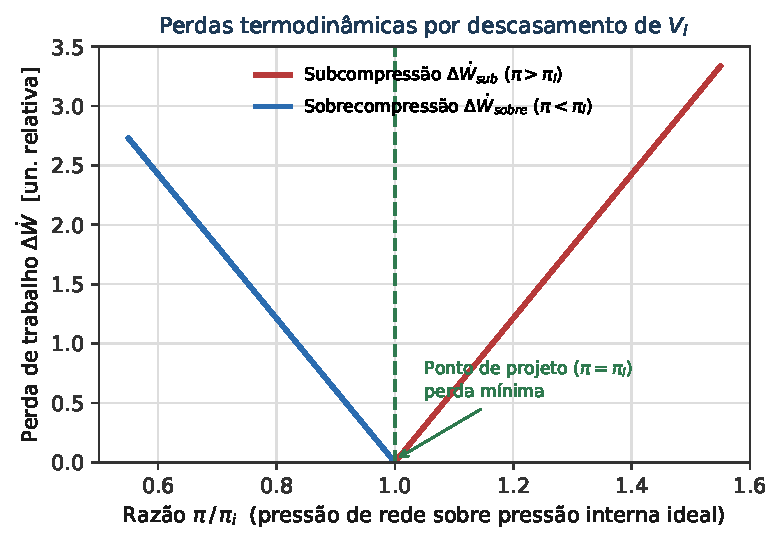
\includegraphics[width=0.60\textwidth]{figuras/fig_5_1_vi_perdas.pdf}
		\caption[Perdas termodinâmicas por sub e sobrecompressão]{Perdas termodinâmicas por sub/sobrecompressão em função do descasamento entre a razão de pressão real e a razão interna ideal do rotor.}
		\label{fig:5-1}
	\end{figure}

	O Gêmeo Digital deve computar continuamente qual regime está ativo comparando $\pi$ medido com $\pi_i$ de projeto, pois essa perda — e não apenas o vazamento por folgas já modelado adiante — é responsável por parte significativa do desvio entre a eficiência isentrópica real e a ideal em condições de operação fora do ponto de projeto (ex.: variação sazonal da contrapressão de rede ou operação em carga parcial).

	\subsection{\textbf{Resfriamento e Separação de Condensado}}
	\begin{itemize}
		\item \textbf{Resfriador intermediário e final (\textit{intercooler} e \textit{aftercooler}):} Trocadores de calor que removem a energia térmica da compressão. A taxa de calor removido, na Equação~\eqref{eq:s5-10}, segue a forma padrão de projeto de trocadores: coeficiente global de transferência ($U$) vezes área de troca térmica ($A$) vezes a diferença de temperatura média logarítmica ($\Delta T_{\text{LMTD}}$, detalhada no Capítulo de Dinâmica do Intercooler):
		\begin{equation}\label{eq:s5-10}
 \dot{Q} = U \cdot A \cdot \Delta T_{\text{LMTD}}
\end{equation}
		\item \textbf{Drenagem de Condensado:} A umidade removida ($\dot{m}_{\text{cond}}$) é calculada pela variação da razão de umidade $W_h$, na Equação~\eqref{eq:s5-11}:
		\begin{equation}\label{eq:s5-11}
 \dot{m}_{\text{cond}} = \dot{m}_{\text{ar}} \cdot (W_{h,\text{in}} - W_{h,\text{out}}) 
\end{equation}
		\item \textbf{Mecanismo de Falha:} Dreno travado (arraste de água para o estágio seguinte) ou \textit{fouling} (incrustação) no trocador.
		\item \textbf{Detecção:} Sensores de nível capacitivos e queda no coeficiente global de transferência de calor $U$.
	\end{itemize}
	
	\subsection{\textbf{Válvulas de Controle e Segurança}}
	\begin{itemize}
		\item \textbf{Válvula de retenção (\textit{check valve}):} Impede o fluxo reverso do reservatório para o compressor na parada.
		\item \textbf{Válvula de alívio (\textit{blow-down}):} Despressuriza o sistema interno para permitir a partida em vazio (\textit{unloaded start}).
	\end{itemize}
	
	\subsection{\textbf{Equacionamento Integrado e Balanço de Potência}}
	A potência total consumida pelo sistema, monitorada pelo Gêmeo Digital para detecção de desvios, é a soma das demandas termodinâmicas e perdas mecânicas, dada pela Equação~\eqref{eq:s5-12}:

	\begin{equation}\label{eq:s5-12}
	\dot{W}_{\text{total}} = \underbrace{\dot{W}_{\text{LP}} + \dot{W}_{\text{HP}}}_{\text{Trabalho de Compressão}} + \underbrace{P_{\text{loss,gb}}}_{\text{Perdas na Gearbox}} + \underbrace{\dot{W}_{\text{bomba}}}_{\text{Potência de Lubrificação}} + \underbrace{P_{\text{fric}}}_{\text{Atrito nos Mancais}}
\end{equation}
	
	Onde:
	\begin{itemize}
		\item $\dot{W}_{\text{LP}}$ e $\dot{W}_{\text{HP}}$: Trabalho termodinâmico nos estágios de baixa e alta pressão.
		\item $P_{\text{loss,gb}}$: Perdas por engrenamento e ventilação na caixa multiplicadora.
		\item $\dot{W}_{\text{bomba}}$: Potência consumida pela bomba de óleo lubrificante.
		\item $P_{\text{fric}}$: Perdas mecânicas por atrito viscoso nos rolamentos e selos.
	\end{itemize}
	
	\vspace{1em}
	\textbf{Eficiência Global do Sistema:} A Equação~\eqref{eq:s5-13} compara o trabalho mínimo teórico de uma compressão isotérmica ideal (o limite termodinâmico, sem nenhuma perda) contra o trabalho total realmente consumido pelo trem de potência (Equação~\eqref{eq:s5-12}) — quanto mais próximo de 1, mais perto do ideal termodinâmico a máquina está operando:
	\begin{equation}\label{eq:s5-13}
 \eta_{\text{global}} = \frac{\dot{W}_{\text{isotérmico\_ideal}}}{\dot{W}_{\text{total}}}
\end{equation}

	\subsection{\textbf{Pressão Intermediária Ótima entre Estágios}}
	A Equação~\eqref{eq:s5-5} modela o trabalho de cada estágio isoladamente, mas não responde a uma pergunta de projeto e de diagnóstico igualmente relevante: dada uma pressão de sucção $P_1$ fixa e uma pressão de descarga final $P_2$ fixa, em que pressão intermediária $P_{\text{int}}$ o trabalho total dos dois estágios é mínimo? A resposta é a formulação clássica de compressão multiestágio \cite{cengel, moran, hanlon}, obtida somando a Equação~\eqref{eq:s5-5} para os estágios LP e HP e minimizando o trabalho total em relação a $P_{\text{int}}$: com resfriamento intermediário \textbf{perfeito} (o intercooler devolve o ar à mesma temperatura de sucção do estágio LP, $T_{HP,\text{in}} = T_{LP,\text{in}}$) e mesmo índice politrópico $n$ nos dois estágios, o mínimo ocorre exatamente quando as duas razões de pressão são iguais — condição que se resolve na média geométrica das pressões extremas, pela Equação~\eqref{eq:s5-14}:
	\begin{equation}\label{eq:s5-14}
 P_{\text{int}}^{*} = \sqrt{P_1 \cdot P_2}
\end{equation}
	Nesse ponto ótimo, $P_{\text{int}}^{*}$ nada mais é do que a pressão interestágio já instrumentada na matriz do Capítulo 18 — a descarga do estágio LP e a sucção do estágio HP são o mesmo ponto físico, $P_{d,lp} = P_{s,hp}$ (ponto C/D da Tabela~\ref{tab:18-1}) — de modo que a Equação~\eqref{eq:s5-14} não introduz variável nova a instrumentar, apenas um valor de referência contra o qual comparar a leitura existente.

	Na prática, o resfriamento intermediário nunca é perfeito: o intercooler degradado modelado pela Equação~\eqref{eq:s10-5} (queda de $U$ por incrustação) entrega o ar ao estágio HP mais quente do que o projeto original previa ($T_{HP,\text{in}} > T_{LP,\text{in}}$). Isso encarece relativamente o trabalho do estágio HP para qualquer razão de pressão fixada nele — a mesma física da penalidade térmica já quantificada na Equação~\eqref{eq:s10-4} — e desloca o ponto de mínimo para longe da média geométrica simples da Equação~\eqref{eq:s5-14}. O Gêmeo Digital ganha, com isso, um critério adicional e independente de desvio: comparar a pressão interestágio efetivamente operada contra $P_{\text{int}}^{*}$ não diagnostica apenas um estágio isoladamente, mas se a \textbf{alocação de carga} entre LP e HP ainda corresponde ao ponto de projeto de fábrica — um sintoma que nenhum dos dois estágios, olhado sozinho, revela.

	\subsection{\textbf{Perda de Carga na Tubulação Interestágios}}
	Todo o equacionamento deste capítulo até aqui trata $P_{\text{int}}$ como um único valor, comum à descarga do estágio LP, à entrada e à saída do intercooler e à sucção do estágio HP — como se os trechos de tubulação que interligam esses pontos não impusessem queda de pressão própria. Essa simplificação ignora o atrito distribuído do escoamento contra a parede do tubo, mecanismo distinto da perda localizada já modelada para filtro e silenciador (Equação~\eqref{eq:s5-4}): ali a perda vem de uma restrição concentrada num único elemento; aqui vem do comprimento inteiro da linha. A forma clássica de Darcy-Weisbach isola essa diferença mantendo a mesma pressão dinâmica $\rho v^2/2$ já usada na Equação~\eqref{eq:s5-4}, agora multiplicada pela razão comprimento/diâmetro da linha em vez de um coeficiente de perda localizada \cite{white} — Equação~\eqref{eq:s5-15}:
	\begin{equation}\label{eq:s5-15}
 \Delta P_{\text{linha}} = f_D \cdot \frac{L_{\text{linha}}}{D_{\text{linha}}} \cdot \frac{\rho \, v^2}{2}
\end{equation}
	Onde $f_D$ é o fator de atrito de Darcy (função do número de Reynolds e da rugosidade relativa da tubulação \cite{white}), $L_{\text{linha}}$ o comprimento do trecho e $D_{\text{linha}}$ seu diâmetro interno. Cada trecho interestágios (descarga LP$\to$intercooler, intercooler$\to$sucção HP, descarga HP$\to$aftercooler) tem sua própria Equação~\eqref{eq:s5-15}, com $f_D$, $L_{\text{linha}}$ e $D_{\text{linha}}$ específicos daquele trecho. O efeito prático é uma pequena correção à pressão usada nas Equações~\eqref{eq:s5-5}, \eqref{eq:s5-8}/\eqref{eq:s5-9} e~\eqref{eq:s5-14}: a pressão de sucção do estágio seguinte é a pressão de descarga do estágio anterior \textbf{menos} a Equação~\eqref{eq:s5-15} do trecho que os liga, não o mesmo valor de $P_{\text{int}}$ usado até aqui por simplificação. Em linhas curtas e bem dimensionadas dentro da própria base estrutural do pacote (\textit{skid}), essa correção costuma ser pequena frente às demais perdas do capítulo — mas cresce com o desgaste (rugosidade interna por corrosão/incrustação, que eleva $f_D$ ao longo da vida da instalação) e deve ser tratada como mais um sintoma rastreável pelo Gêmeo Digital, não descartada por ser pequena no comissionamento.

	\subsection{\textbf{Perda de Carga Parametrizada em Válvulas de Alívio e Retenção}}

	O catálogo de mecanismos de falha do Capítulo 28 (Seção~28.3) trata a válvula de \textit{blow-off}, a válvula de retenção (\textit{check valve}) e a válvula de segurança e alívio (PSV) como mecanismos \textbf{binários}: a válvula funciona dentro da especificação ou falhou (trava aberta, trava fechada, vaza acima do assento). Essa simplificação deixa de fora o regime intermediário que, na prática, costuma preceder a falha binária — o assento desgasta, a mola perde rigidez por fadiga ou corrosão, ou depósitos se acumulam na sede, e a perda de carga que a válvula impõe ao escoamento cresce de forma gradual muito antes de qualquer travamento. É o mesmo padrão de degradação já modelado para o filtro de admissão (Equação~\eqref{eq:s5-4}) e para a tubulação interestágios (Equação~\eqref{eq:s5-15}) — e a mesma forma clássica de perda de carga localizada se aplica, com um coeficiente próprio de cada válvula, $\zeta_{\text{valv}}$, na Equação~\eqref{eq:s5-16}:

	\begin{equation}\label{eq:s5-16}
	\Delta P_{\text{valv}} = \zeta_{\text{valv}} \cdot \frac{\rho \, v^2}{2}
	\end{equation}

	Como no filtro (Equação~\eqref{eq:s5-4}), $\zeta_{\text{valv}}$ cresce a partir de um valor de referência limpo/novo ($\zeta_{\text{valv,ref}}$) conforme a válvula degrada — mas, diferente do filtro, cuja perda é permanentemente exposta ao escoamento principal, cada válvula deste grupo só é atravessada por vazão em condições específicas (a PSV só abre acima da pressão de ajuste; a de retenção conduz continuamente, mas em um único sentido; o \textit{blow-off} só atua durante alívio de partida ou parada). O sinal de degradação, portanto, não é uma leitura contínua como $\Delta P_{ic}$ do intercooler (ponto D da Tabela~\ref{tab:18-1}), mas o desvio entre a perda de carga observada no instante em que a válvula efetivamente conduz e o valor de referência esperado para aquela vazão — exigindo, tal qual $\zeta_{\text{ref}}$ do filtro (Seção~28.2), um canal de medição de pressão diferencial dedicado, hoje ausente da matriz da Tabela~\ref{tab:18-1}.

	Com esse coeficiente definido, a mesma técnica de estimação conjunta de estado e parâmetro que identifica $K$, $\eta_{\text{mec}}$ e $\zeta_{\text{ref}}$ (Seção~28.1) se estende naturalmente a $\zeta_{\text{valv}}$: basta incluí-lo no vetor $\Lambda$ da Equação~\eqref{eq:s28-1}, desde que exista, para aquela válvula específica, a medição de $\Delta P_{\text{valv}}$ que torna o parâmetro observável — a mesma condição discutida na Seção de Condição de Observabilidade do Capítulo 21, agora aplicada a um quarto parâmetro estático em vez dos três originais.

	\vspace{1em}
	\hrule
	\vspace{1em}

	\textbf{Diretriz Técnica Final:} A Equação~\eqref{eq:s5-13} consolida todo o capítulo em um único KPI de eficiência global — mas seu valor só é confiável se cada termo de perda (folga interna via $V_i$, gearbox, bomba de óleo) estiver sendo medido ou estimado corretamente; um $\eta_{\text{global}}$ isolado sem essa rastreabilidade componente-a-componente é apenas um número, não um diagnóstico. A Equação~\eqref{eq:s5-14} acrescenta um segundo eixo de leitura, ortogonal ao primeiro: mesmo com $\eta_{\text{global}}$ nominal, uma pressão interestágio deslocada do ótimo indica que a carga entre os dois estágios está mal balanceada — tipicamente o primeiro sinal observável de um intercooler em degradação, antes mesmo que a Equação~\eqref{eq:s10-4} feche o diagnóstico. A Equação~\eqref{eq:s5-15} fecha a última lacuna de perda de carga do trem primário: uma tendência de alta em $f_D$ para o mesmo ponto de operação, isolada da leitura de $P_{\text{int}}$, é sintoma de degradação da própria tubulação (corrosão, incrustação interna), independente de qualquer coisa que esteja acontecendo no intercooler ou nos estágios. A Equação~\eqref{eq:s5-16} estende essa mesma lógica de perda de carga localizada às válvulas de alívio e retenção, hoje tratadas como falha binária no catálogo do Capítulo 28 — uma tendência de alta em $\zeta_{\text{valv}}$ é o análogo, para essas válvulas, do que a tendência de alta em $\zeta_{\text{ref}}$ já representa para o filtro de admissão.

	% --- Fim do Capítulo 5 ---
	
	% --- Início do Capítulo 6: Engenharia do Trem de Transmissão e Matriz de Confiabilidade ---
	
	\clearpage
	\section{\textbf{Engenharia do Trem de Transmissão e Matriz de Confiabilidade}}
	
	Este capítulo detalha a modelagem física do sistema de transmissão de potência, integrando a cinemática da caixa multiplicadora com a dinâmica de falhas mecânicas. O objetivo é estabelecer o modelo de referência para o Gêmeo Digital, permitindo o isolamento entre perdas mecânicas e termodinâmicas.
	
	\subsection{\textbf{Cinemática e Fluxo de Potência}}
	A transferência de energia do motor para os rotores de compressão (LP e HP) é governada pela conservação do momento angular e pelas eficiências de interface.
	\begin{itemize}
		\item \textbf{Balanço de Potência Instantânea:} A Equação~\eqref{eq:s6-1} afirma que toda a potência entregue pelo motor (já descontada a perda no acoplamento) é distribuída entre o trabalho de compressão nos dois estágios ($P_{\text{LP}}$, $P_{\text{HP}}$), as perdas da gearbox e um termo de aceleração angular do sistema — este último relevante apenas em transientes, pois some quando a rotação é constante ($d\omega/dt = 0$):
		\begin{equation}\label{eq:s6-1}
 P_{\text{mot}} \cdot \eta_{\text{acopl}} = P_{\text{LP}} + P_{\text{HP}} + P_{\text{loss,gb}} + I_{\text{sys}} \cdot \omega \cdot \frac{d\omega}{dt}
\end{equation}
		Onde $P_{\text{loss,gb}}$ é a potência dissipada na caixa multiplicadora e $I_{\text{sys}}$ é o momento de inércia equivalente referido ao eixo do motor.
		\item \textbf{Relação de Transmissão e Velocidades:} A razão de engrenamento entre coroa e pinhão eleva a rotação do motor até a velocidade de operação dos rotores, conforme a Equação~\eqref{eq:s6-2}:
		\begin{equation}\label{eq:s6-2}
 \omega_{\text{rotor}} = \omega_{\text{mot}} \cdot \frac{Z_{\text{coroa}}}{Z_{\text{pinhão}}} 
\end{equation}
	\end{itemize}
	
	\subsection{\textbf{Modelagem de Perdas Parasitas na Gearbox}}
	As perdas na caixa multiplicadora variam dinamicamente com a carga, rotação e viscosidade do óleo $\mu(T)$.
	\begin{itemize}
		\item \textbf{Perdas por Engrenamento ($P_{\text{mesh}}$):} A Equação~\eqref{eq:s6-3} modela a fração da potência transmitida ($P_{\text{trans}}$) que se converte em atrito no contato entre os dentes, escalada pelo coeficiente de atrito e por um termo geométrico dependente do ângulo de pressão da engrenagem:
		\begin{equation}\label{eq:s6-3}
 P_{\text{mesh}} = f_{\text{fric}} \cdot P_{\text{trans}} \cdot \sec(\phi)
\end{equation}
		Onde $f_{\text{fric}}$ é o coeficiente de atrito (função da rugosidade e lubrificação) e $\phi$ é o ângulo de pressão — a força normal sobre o flanco do dente escala com $\sec(\phi) = 1/\cos(\phi)$ (normas AGMA/ISO), não com o arco-cosseno de $\phi$.
		\item \textbf{Perdas por Agitação e Ventilação ($P_{\text{windage}}$):} O arrasto viscoso do óleo contra as engrenagens em rotação cresce com o cubo da velocidade angular, pela Equação~\eqref{eq:s6-4}:
		\begin{equation}\label{eq:s6-4}
 P_{\text{windage}} = C_w \cdot \rho_{\text{óleo}} \cdot \omega^3 \cdot D^5 
\end{equation}
		Onde $C_w$ é o coeficiente de arrasto e $D$ o diâmetro das engrenagens.
	\end{itemize}
	
	\subsection{\textbf{Matriz de Mecanismos de Falha e Indicadores Digitais}}
	A Tabela~\ref{tab:6-1} correlaciona cada componente físico da caixa multiplicadora ao seu modo de falha característico e ao indicador digital que permite detectá-lo. A leitura é por linha: o componente identifica \textit{onde} a falha ocorre; o mecanismo descreve \textit{como} ela progride fisicamente; e o indicador digital é a grandeza — medida ou inferida — cujo desvio denuncia a progressão antes que ela atinja o limite funcional. Essa estrutura de três colunas se repete nas matrizes de falha dos capítulos seguintes, e é o que permite ao Gêmeo Digital passar de um diagnóstico genérico (``vibração alta'') para uma hipótese de causa raiz específica.
	
	\begin{table}[h!tbp]
		\centering
		\resizebox{\textwidth}{!}{
		\begin{tabular}{l l l l}
			\toprule
			\textbf{Componente} & \textbf{Mecanismo de Falha} & \textbf{Causa Raiz} & \textbf{Indicador Digital} \\ \midrule
			Acoplamento & Desalinhamento & Assentamento / Térmico & Pico em $2 \times \text{RPM}$ \\
			Acoplamento & Fadiga do Elemento & Sobrecarga & Resíduo de torque $r_{\tau}$ \\
			Engrenagens & \textit{Pitting} (Fadiga) & Carga cíclica & Bandas laterais em $GMF$ \\
			Engrenagens & \textit{Scuffing} & Falha de filme de óleo & $\uparrow T$ óleo de retorno \\
			Mancais & Desgaste de Metal & Contaminação & $\downarrow P_{\text{óleo}}$ e vibração \\
			Selos & Desgaste Labirinto & Vibração excessiva & $\downarrow \eta_{\text{vol}}$ e $\uparrow T_{\text{suc}}$ \\ \bottomrule
		\end{tabular}
		}
		\caption[Mecanismos de falha da caixa multiplicadora]{Mecanismos de falha do acoplamento, engrenagens, mancais e selos da caixa multiplicadora, com o respectivo indicador digital monitorado pelo Gêmeo Digital.}
		\label{tab:6-1}
	\end{table}
	
	\subsection{\textbf{Dinâmica de Eixos e Sincronismo (Timing)}}
	Em compressores isentos de óleo, as engrenagens de sincronismo garantem que os rotores mantenham a folga nominal sem contato físico.
	\begin{itemize}
		\item \textbf{Rigidez Torcional do Eixo ($k_t$):} A Equação~\eqref{eq:s6-5} estima a torção angular ($\Delta \theta$) que o eixo sofre ao transmitir um torque $\tau$ ao longo de um comprimento $L$, em função da rigidez do material — módulo de cisalhamento $G$ e momento polar de inércia da seção transversal $J_p$ (ambos parâmetros geométricos/de material fixos do eixo; o subscrito evita colidir com a função de custo $J$ do MPC/PSO, usada na Parte II):
		\begin{equation}\label{eq:s6-5}
 \Delta \theta = \frac{\tau \cdot L}{G \cdot J_p}
\end{equation}
		\item \textbf{Risco Crítico:} Se $\Delta \theta$ exceder a folga angular (\textit{backlash}) de projeto, ocorre contato metal-metal. O Gêmeo Digital detecta isso via \textit{Motor Current Signature Analysis} (MCSA).
	\end{itemize}
	
	\subsection{\textbf{Diagnóstico por Resíduos de Potência}}
	O Gêmeo Digital calcula o resíduo mecânico ($r_{\text{mec}}$) para isolar anomalias, pela Equação~\eqref{eq:s6-6}:
	\begin{equation}\label{eq:s6-6}
 r_{\text{mec}} = P_{\text{real}} - \left( \frac{\dot{W}_{\text{LP}} + \dot{W}_{\text{HP}}}{\eta_{\text{mec,modelo}}} \right) 
\end{equation}
	\begin{itemize}
		\item $r_{\text{mec}} > 0$: Indica aumento de atrito (falha de rolamento ou engrenagem).
		\item $r_{\text{mec}} < 0$: Indica erro de calibração ou fuga interna massiva.
	\end{itemize}
	
	\subsection{\textbf{Frequências de Monitoramento}}
	As frequências características usadas ao longo deste documento como referência de diagnóstico espectral seguem diretamente da cinemática do trem de potência — a Equação~\eqref{eq:s6-7} converte a rotação medida (RPM) na frequência de giro do eixo ($f_r$) e, a partir dela, na frequência de engrenamento ($GMF$, aqui $f_g$) pelo número de dentes $Z$:
	\begin{equation}\label{eq:s6-7}
 f_r = \frac{\text{RPM}}{60} \quad ; \quad f_g = f_r \cdot Z
\end{equation}

	\vspace{1em}
	\textbf{Equação de Torque de Referência:} A Equação~\eqref{eq:s6-8} sintetiza tudo o que foi apresentado neste capítulo em um único torque teórico esperado no eixo do motor: soma o trabalho politrópico de compressão dos dois estágios (LP e HP) com as perdas da gearbox, e converte de potência para torque dividindo pela rotação do motor e pela eficiência da caixa multiplicadora — este é o valor de referência contra o qual o torque real medido é comparado no resíduo mecânico $r_{\text{mec}}$ da Equação~\eqref{eq:s6-6}:
	\begin{equation}\label{eq:s6-8}
 \boxed{\tau_{\text{ref}} = \frac{1}{\omega_{\text{mot}} \cdot \eta_{\text{gb}}} \left[ \sum_{i=1}^{2} \left( \frac{n}{n-1} P_{\text{in},i} \dot{V}_{\text{in},i} \left( \pi_i^{\frac{n-1}{n}} - 1 \right) \right) + P_{\text{loss,gb}} \right]}
\end{equation}

	\vspace{1em}
	\hrule
	\vspace{1em}

	\textbf{Diretriz Técnica Final:} O torque de referência da Equação~\eqref{eq:s6-8} é o valor teórico esperado a partir das condições de processo; o resíduo mecânico ($r_{\text{mec}}$) desta seção só é um diagnóstico útil se comparado continuamente contra esse torque de referência recalculado em tempo real — nunca contra um valor de projeto fixo.

	% --- Fim do Capítulo 6 ---
	
	% --- Início do Capítulo 7: Sistema de Lubrificação e Dinâmica de Mancais (Versão Expandida) ---
	
	\clearpage
	\section{\textbf{Sistema de Lubrificação, Arrefecimento de Óleo e Dinâmica de Mancais}}
	
	Este capítulo detalha a modelagem do sistema de suporte vital dos componentes rotativos. Em compressores isentos de óleo, o lubrificante é responsável pela integridade da caixa multiplicadora e dos mancais de alta rotação, atuando como o principal meio de transporte de calor dissipado por atrito mecânico.
	
	\subsection{\textbf{Acionamento e Consumo Energético da Bomba de Óleo}}
	O sistema utiliza uma bomba de deslocamento positivo acionada por um motor elétrico independente, permitindo as funções críticas de pré-lubrificação e pós-lubrificação (\textit{standby cooling}).
	\begin{itemize}
		\item \textbf{Potência Elétrica Consumida ($P_{\text{elec,pump}}$):} A Equação~\eqref{eq:s7-1} iguala duas formas de calcular a mesma potência — o lado elétrico (tensão $V$, corrente $I$ e fator de potência $\cos\phi$ trifásicos, medidos no painel) e o lado hidráulico (vazão de óleo vezes o diferencial de pressão da bomba, dividido pela eficiência total). Comparar os dois lados é justamente o que permite detectar falha antes que ela se manifeste mecanicamente:
		\begin{equation}\label{eq:s7-1}
 P_{\text{elec,pump}} = \sqrt{3} \cdot V \cdot I \cdot \cos \phi = \frac{\dot{V}_{\text{oil}} \cdot \Delta P_{\text{pump}}}{\eta_{\text{total,pump}}}
\end{equation}
		\item \textbf{Indicador de Saúde:} O Gêmeo Digital monitora o desvio de corrente $\Delta I = I_{\text{medido}} - I_{\text{modelo}}(T_{\text{oil}})$. Um aumento em $\Delta I$ sem aumento de pressão indica falha iminente no enrolamento do motor ou travamento mecânico da bomba.
	\end{itemize}
	
	\subsection{\textbf{Reologia do Lubrificante e Perda de Carga no Circuito}}
	A viscosidade dinâmica $\mu(T)$ é o parâmetro central para o cálculo de perdas e proteção de película.
	\begin{itemize}
		\item \textbf{Equação de Vogel \cite{vogel} para Viscosidade:} A Equação~\eqref{eq:s7-2} descreve a queda não linear da viscosidade dinâmica com a temperatura:
		\begin{equation}\label{eq:s7-2}
 \mu(T) = a \cdot \exp \left( \frac{b}{T - c} \right) 
\end{equation}
		Onde $a$, $b$ e $c$ são constantes empíricas obtidas por ajuste de curva aos dados do fabricante do lubrificante (não possuem significado físico individual — apenas a combinação reproduz a curva $\mu \times T$ medida). A Figura~\ref{fig:7-1} ilustra a forma típica dessa curva: a viscosidade cai de forma acentuadamente não linear com o aumento da temperatura, e é justamente essa não linearidade que torna a Equação~\eqref{eq:s7-2} necessária em vez de uma simples interpolação linear.

		\begin{figure}[h!tbp]
			\centering
			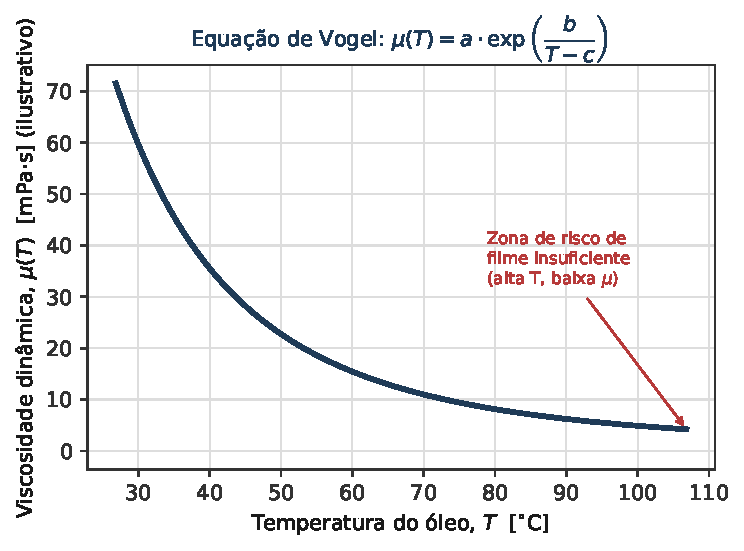
\includegraphics[width=0.60\textwidth]{figuras/fig_7_1_vogel.pdf}
			\caption[Curva de viscosidade de Vogel]{Curva de viscosidade de Vogel — queda não linear da viscosidade com a temperatura (valores ilustrativos).}
			\label{fig:7-1}
		\end{figure}

		\item \textbf{Perda de Carga no Filtro ($\Delta P_{\text{filt}}$):} Modelada pela lei de Darcy-Forchheimer para meios porosos, na Equação~\eqref{eq:s7-3}:
		\begin{equation}\label{eq:s7-3}
 \Delta P_{\text{filt}} = \underbrace{A \cdot \mu \cdot v}_{\text{Componente Viscosa}} + \underbrace{B \cdot \rho \cdot v^2}_{\text{Componente Inercial}} 
\end{equation}
		Onde $A$ e $B$ são coeficientes de permeabilidade e inércia do elemento filtrante.
	\end{itemize}
	
	\subsection{\textbf{Dinâmica de Mancais e Balanço Térmico}}
	Os mancais de alta rotação dissipam energia por cisalhamento viscoso, elevando a temperatura do óleo.
	\begin{itemize}
		\item \textbf{Potência de Atrito nos Mancais ($P_{\text{fric,brg}}$):} A Equação~\eqref{eq:s7-4} descreve a dissipação viscosa dentro do filme de óleo do mancal: cresce com a viscosidade $\mu$, com o quadrado da velocidade angular $\omega$, com o cubo do raio do mancal $R$ e com o comprimento axial $L$, mas é inversamente proporcional à espessura do filme lubrificante $e_{\text{filme}}$ — um filme mais fino dissipa mais energia por atrito, com $\xi$ como coeficiente de forma do mancal:
		\begin{equation}\label{eq:s7-4}
 P_{\text{fric,brg}} = \xi \cdot \frac{\mu \cdot \omega^2 \cdot R^3 \cdot L}{e_{\text{filme}}}
\end{equation}
		Onde $e_{\text{filme}}$ é a espessura da película lubrificante (usa-se $e_{\text{filme}}$ em vez de $h$ para não colidir com a entalpia específica dos capítulos de termodinâmica).
		\item \textbf{Elevação de Temperatura do Óleo ($\Delta T_{\text{oil}}$):} A Equação~\eqref{eq:s7-5} converte a potência de atrito total num aumento de temperatura, via vazão mássica e calor específico do óleo:
		\begin{equation}\label{eq:s7-5}
 \Delta T_{\text{oil}} = \frac{P_{\text{fric,total}}}{\dot{m}_{\text{oil}} \cdot c_{p,\text{oil}}} 
\end{equation}
		O Gêmeo Digital utiliza este balanço para validar se o fluxo de óleo ($\dot{m}_{\text{oil}}$) está adequado para a carga térmica atual.
	\end{itemize}
	
	\subsection{\textbf{Gerenciamento Térmico e Válvula Termostática}}
	O controle da temperatura é realizado via trocador de calor e uma válvula termostática de três vias.
	\begin{itemize}
		\item \textbf{Efetividade do Resfriador ($\epsilon$):} A Equação~\eqref{eq:s7-6} mede quanto da queda de temperatura teoricamente possível o resfriador realmente entrega — a razão entre a queda real do óleo ($T_{\text{oil,in}} - T_{\text{oil,out}}$) e a máxima queda termodinamicamente possível, limitada pela temperatura de entrada da água de resfriamento ($T_{\text{oil,in}} - T_{\text{water,in}}$):
		\begin{equation}\label{eq:s7-6}
 \epsilon = \frac{T_{\text{oil,in}} - T_{\text{oil,out}}}{T_{\text{oil,in}} - T_{\text{water,in}}}
\end{equation}
		\item \textbf{Lógica da Válvula Termostática:} O modelo prevê a posição da válvula baseada no \textit{setpoint} de operação. Se $T_{\text{oil}}$ sobe e a válvula está 100\% aberta para o resfriador sem queda de temperatura, o modelo identifica \textit{fouling} (incrustação) no trocador.
	\end{itemize}
	
	\subsection{\textbf{Matriz de Mecanismos de Falha do Sistema de Óleo}}
	A Tabela~\ref{tab:7-1} associa cada componente do circuito de lubrificação ao seu modo de falha típico e ao indicador digital correspondente, usado pelo Gêmeo Digital para diagnóstico automático.
	\begin{table}[h!tbp]
		\centering
		\small
		\renewcommand{\arraystretch}{1.5}
		\begin{tabular}{l l l}
			\toprule
			\textbf{Componente} & \textbf{Mecanismo de Falha} & \textbf{Indicador no Gêmeo Digital} \\ \midrule
			\textbf{Motor da Bomba} & Sobrecarga / Curto-circuito & $\uparrow I_{\text{pump}}$ (Resíduo de Corrente) \\
			\textbf{Bomba de Óleo} & Cavitação ou Desgaste & $\downarrow P_{\text{oil}}$ vs $\uparrow \text{RPM}$ da Bomba \\
			\textbf{Filtro de Óleo} & Colmatagem (Saturação) & $\uparrow \Delta P_{\text{filt}}$ (Normalizado pela viscosidade) \\
			\textbf{Resfriador} & Incrustação (\textit{Fouling}) & $\downarrow \epsilon$ (Queda na Efetividade Térmica) \\
			\textbf{Mancais} & Desgaste de Metal Patente & $\uparrow T_{\text{brg}}$ e $\uparrow$ Vibração de Alta Frequência \\ \bottomrule
		\end{tabular}
		\caption[Mecanismos de falha do sistema de lubrificação]{Matriz de mecanismos de falha do sistema de lubrificação (bomba, filtro, resfriador e mancais).}
		\label{tab:7-1}
	\end{table}
	
	\subsection{\textbf{Equacionamento de Diagnóstico por Resíduos}}
	O isolamento de falhas é realizado através do cálculo de resíduos em tempo real:
	\begin{itemize}
		\item \textbf{Resíduo de Pressão ($r_{\Delta P}$):} $ \Delta P_{\text{real}} - \Delta P_{\text{modelo}}(\dot{V}, \mu) $
		\item \textbf{Resíduo de Potência da Bomba ($r_{P}$):} $ P_{\text{elec,medido}} - P_{\text{hidráulico,calc}} $
		\item \textbf{Resíduo Térmico ($r_{\epsilon}$):} $ \epsilon_{\text{real}} - \epsilon_{\text{modelo}} $
	\end{itemize}
	
	\vspace{1em}
	\textbf{Estado de Saúde do Sistema de Óleo ($SOH_{\text{oil}}$):} A Equação~\eqref{eq:s7-7} consolida três indicadores normalizados — desvio de viscosidade, limite de perda de carga sobre perda real no filtro, e efetividade real sobre nominal do resfriador — cada um variando entre 0 (crítico) e 1 (saudável), e toma o menor valor entre os três como saúde global do sistema. O termo de viscosidade não pode ser a razão direta $\mu_{\text{real}}/\mu_{\text{nom}}$: essa razão só penaliza o afinamento do óleo ($\mu_{\text{real}} < \mu_{\text{nom}}$), mas o envelhecimento por oxidação e formação de borras/vernizes eleva a viscosidade ($\mu_{\text{real}} > \mu_{\text{nom}}$), o que produziria razão $>1$ e mascararia a degradação. O indicador $\Theta_\mu$ penaliza o desvio \textbf{bilateral} em relação à tolerância de projeto $\text{Tol}_\mu$:
	\begin{equation}\label{eq:s7-7}
 \Theta_\mu = \max\left(0,\ 1 - \frac{|\mu_{\text{real}} - \mu_{\text{nom}}|}{\text{Tol}_\mu}\right) \qquad \boxed{SOH_{\text{oil}} = \min \left( \Theta_\mu, \frac{\Delta P_{\text{lim}}}{\Delta P_{\text{real}}}, \frac{\epsilon_{\text{real}}}{\epsilon_{\text{nom}}} \right)}
\end{equation}

	\subsection{\textbf{Análise Físico-Química do Óleo (Canal Laboratorial \textit{Offline})}}
	As três entradas da Equação~\eqref{eq:s7-7} — viscosidade, perda de carga e efetividade térmica — têm em comum o fato de serem todas medidas \textbf{online}, em tempo real, por sensores permanentes de campo. Esse canal é rápido, mas cego a um tipo de degradação: a deterioração química do próprio óleo, que só se manifesta na viscosidade ou no $\Delta P$ depois de já ter avançado o suficiente para alterar as propriedades físicas do fluido. A prática consolidada de manutenção preditiva \cite{mobley} complementa o monitoramento online com uma tríade laboratorial \textbf{offline}, amostrada periodicamente:
	\begin{itemize}
		\item \textbf{Número de Acidez Total (TAN):} Medido por titulação potenciométrica \cite{astmd664}, quantifica os subprodutos ácidos da oxidação do óleo em serviço. Uma tendência de alta do TAN antecede a queda de viscosidade e a formação de vernizes/borras que eventualmente entopem o filtro — é o primeiro sinal químico de que o óleo está no fim da vida útil, ainda quando $SOH_{\text{oil}}$ da Equação~\eqref{eq:s7-7} continua em 1.
		\item \textbf{Água no Óleo:} Medida por titulação coulométrica de Karl Fischer \cite{astmd6304}, quantifica a contaminação por umidade — relevante mesmo em circuito fechado, pois condensação interna (partida a frio, variação de temperatura ambiente offshore) introduz água sem qualquer falha de vedação externa. Água dissolvida acelera a própria oxidação que o TAN mede, tornando os dois ensaios complementares, não redundantes.
		\item \textbf{Contagem de Partículas (Código ISO 4406):} Reporta a concentração de partículas sólidas em três faixas de tamanho ($\ge 4\,\mu\text{m}$, $\ge 6\,\mu\text{m}$, $\ge 14\,\mu\text{m}$) como um código de três números \cite{iso4406}. É o canal que detecta desgaste abrasivo incipiente de engrenagens e rolamentos — partículas metálicas no óleo — antes que esse desgaste produza qualquer assinatura vibracional detectável pelos acelerômetros já instrumentados no ponto B da Tabela~\ref{tab:18-1}.
	\end{itemize}
	Os três ensaios entram no Gêmeo Digital como tendências de baixa frequência (tipicamente uma amostra a cada troca programada ou intervalo fixo, não em tempo real), alimentando o mesmo princípio de variável \textit{real} versus \textit{virtual} já estabelecido na matriz do Capítulo 18 — mas como uma terceira categoria, intermediária entre as duas: medição real, porém de baixíssima taxa de amostragem, o que exige do modelo uma lógica de interpolação/extrapolação de tendência distinta da usada para os sensores contínuos.

	\vspace{1em}
	\hrule
	\vspace{1em}

	\textbf{Diretriz Técnica Final:} O uso do operador $\min(\cdot)$ na Equação~\eqref{eq:s7-7} é deliberado — o Estado de Saúde do sistema de óleo é sempre ditado pelo pior indicador entre viscosidade, perda de carga e efetividade térmica, nunca por uma média entre eles, refletindo que uma única falha isolada já compromete a lubrificação como um todo. A tríade laboratorial desta seção não substitui $SOH_{\text{oil}}$ — ela o antecede: TAN, água e contagem de partículas tipicamente sinalizam degradação química e desgaste abrasivo semanas ou meses antes que a Equação~\eqref{eq:s7-7} caia, porque medem a causa quando o canal online ainda só vê o efeito.

	% --- Fim do Capítulo 7 ---
	
	% --- Início do Capítulo 8: Dinâmica de Transmissão e Sincronismo (Versão Integral) ---
	
	\clearpage
	\section{\textbf{Dinâmica de Transmissão, Sincronismo e Integridade de Engrenamentos}}
	
	Este capítulo detalha a modelagem física da transmissão de potência em compressores de múltiplos estágios, focando na cinemática de engrenamento, na integridade estrutural dos dentes, na dinâmica de rolamentos de precisão e nos efeitos de desalinhamento.
	
	\subsection{\textbf{Cinemática da Transmissão e Relações de Velocidade}}
	Em uma configuração de motor único com caixa integrada, a coroa principal (\textit{Bull Gear}) aciona simultaneamente os pinhões dos estágios de Baixa Pressão (LP) e Alta Pressão (HP). O sincronismo interno de cada par de rotores é garantido por engrenagens de \textit{timing} dedicadas. A Figura~\ref{fig:8-1} esquematiza essa cinemática: a coroa central, acionada pelo motor, engrena simultaneamente com os dois pinhões (LP e HP), cada um girando a uma velocidade diferente conforme sua própria relação de dentes — exatamente a lógica capturada pela Equação~\eqref{eq:s8-1} a seguir.

	\begin{figure}[h!tbp]
		\centering
		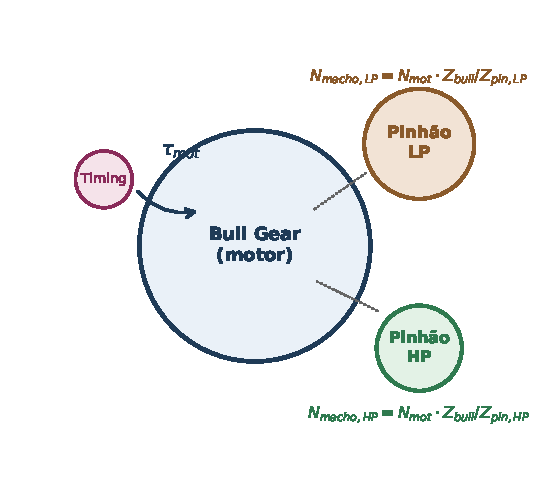
\includegraphics[width=0.75\textwidth]{figuras/fig_8_1_gearbox.pdf}
		\caption[Esquema cinemático da caixa multiplicadora]{Esquema cinemático simplificado da caixa multiplicadora: coroa (\textit{bull gear}) acionando os pinhões LP e HP, com engrenagem de sincronismo (\textit{timing}).}
		\label{fig:8-1}
	\end{figure}

	\begin{itemize}
		\item \textbf{Relação de Multiplicação dos Estágios ($i$):}
		A rotação do rotor macho de cada estágio ($N_{\text{macho}}$) é determinada pela geometria da \textit{gearbox}:
		\begin{equation}\label{eq:s8-1}
 N_{\text{macho,LP}} = N_{\text{mot}} \cdot \left( \frac{Z_{\text{bull}}}{Z_{\text{pin,LP}}} \right) \quad ; \quad N_{\text{macho,HP}} = N_{\text{mot}} \cdot \left( \frac{Z_{\text{bull}}}{Z_{\text{pin,HP}}} \right) 
\end{equation}
		Onde $Z_{\text{bull}}$ é o número de dentes da coroa e $Z_{\text{pin}}$ o do pinhão.
		
		\item \textbf{Sincronismo Interno (Relação Macho-Fêmea):}
		As engrenagens de sincronismo (\textit{timing gears}) impõem a relação de velocidades necessária para evitar o contato entre os lóbulos, pela Equação~\eqref{eq:s8-2}:
		\begin{equation}\label{eq:s8-2}
 N_{\text{fêmea}} = N_{\text{macho}} \cdot \left( \frac{Z_{\text{sync,macho}}}{Z_{\text{sync,fêmea}}} \right) 
\end{equation}
		O Gêmeo Digital monitora o erro de fase angular $\Delta \phi = \theta_{\text{macho}} - G_s \theta_{\text{fêmea}}$ para prever colisões.
	\end{itemize}
	
	\subsection{\textbf{Equacionamento de Torque e Balanço de Potência}}
	O torque total fornecido pelo motor ($\tau_{\text{mot}}$) é distribuído entre os estágios, considerando as eficiências de engrenamento ($\eta_{\text{gb}}$).
	\begin{itemize}
		\item \textbf{Balanço de Torque no Eixo da Coroa:} A Equação~\eqref{eq:s8-3} reparte o torque do motor (já descontada a eficiência de engrenamento $\eta_{\text{gb}}$) entre os dois pinhões, cada torque de estágio dividido pela sua respectiva relação de transmissão ($i_{\text{LP}}$, $i_{\text{HP}}$):
		\begin{equation}\label{eq:s8-3}
 \tau_{\text{mot}} \cdot \eta_{\text{gb}} = \frac{\tau_{\text{LP}}}{i_{\text{LP}}} + \frac{\tau_{\text{HP}}}{i_{\text{HP}}}
\end{equation}
		Onde $\tau_{\text{LP}}$ e $\tau_{\text{HP}}$ são os torques requeridos pela compressão. Desvios neste balanço indicam anomalias mecânicas (ex: atrito excessivo em selos) ou depósitos nos rotores.
	\end{itemize}
	
	\subsection{\textbf{Dinâmica de Rolamentos e Diagnóstico de Vida Útil}}
	Os pinhões de alta velocidade são suportados por rolamentos de precisão, cuja vida útil nominal ($L_{10h}$) é modelada em função da carga equivalente $P$:
	\begin{itemize}
		\item \textbf{Carga Equivalente e Vida Útil:} A Equação~\eqref{eq:s8-4} combina as cargas radial e axial reais em uma única carga equivalente $P$ (norma ISO 281), e usa essa carga equivalente para projetar quantas horas de operação o rolamento suporta antes de 10\% da população falhar por fadiga:
		\begin{equation}\label{eq:s8-4}
 P = X \cdot F_r + Y \cdot F_a \implies L_{10h} = \frac{10^6}{60 \cdot N_{\text{rot}}} \left( \frac{C}{P} \right)^p
\end{equation}
		Onde $F_r$ e $F_a$ são as cargas radial e axial medidas/estimadas no rolamento, $X$ e $Y$ são os fatores radial e axial de carga dinâmica (tabelados pelo fabricante do rolamento em função da razão $F_a/F_r$), $N_{\text{rot}}$ é a rotação do eixo em RPM (para não colidir com $N$ usado como número de compressores na frota, Cap. 14), $C$ é a capacidade de carga dinâmica e $p$ é o expoente de vida (3 para esferas, 10/3 para rolos). Por ser uma lei de potência com expoente $p=3$, a vida do rolamento é extremamente sensível à carga — a Figura~\ref{fig:8-3} mostra que dobrar a carga reduz a vida a aproximadamente 1/8, motivo pelo qual pequenos desalinhamentos ou desbalanceamentos que elevam $P$ têm impacto desproporcional na confiabilidade do mancal.

		\begin{figure}[h!tbp]
			\centering
			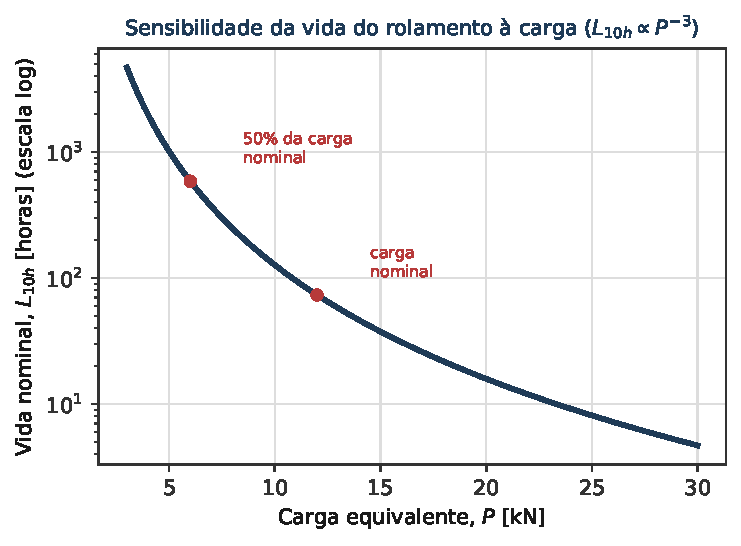
\includegraphics[width=0.60\textwidth]{figuras/fig_8_3_l10h.pdf}
			\caption[Sensibilidade da vida do rolamento à carga]{Sensibilidade da vida nominal do rolamento ($L_{10h}$) à carga equivalente — note a escala logarítmica no eixo vertical.}
			\label{fig:8-3}
		\end{figure}

		\item \textbf{Indicadores de Falha:} O modelo monitora frequências de pista externa (BPFO), interna (BPFI) e elementos rolantes (BSF), utilizando a \textit{Curtose} e o \textit{Fator de Crista} para identificar o início de lascamento (\textit{spalling}).
	\end{itemize}

	\subsection{\textbf{Rotordinâmica e Velocidade Crítica}}
	A vida útil dos rolamentos (Equação~\eqref{eq:s8-4}) descreve o desgaste por fadiga de contato, mas não protege por si só contra o modo de falha mais súbito de eixos de alta rotação: a ressonância lateral. Os pinhões do estágio HP operam tipicamente acima da primeira velocidade crítica, exigindo que o Gêmeo Digital trate o eixo como um sistema rotordinâmico, não apenas como uma carga estática sobre o mancal.
	\begin{itemize}
		\item \textbf{Velocidade Crítica (Modelo de Jeffcott):} Aproximando o conjunto eixo-pinhão como um rotor de Jeffcott (massa concentrada $m$ sobre um eixo de rigidez lateral $k_s$, apoiado em mancais de rigidez $k_b$), a primeira velocidade crítica é dada pela Equação~\eqref{eq:s8-5}:
		\begin{equation}\label{eq:s8-5}
 \omega_{cr} = \sqrt{\frac{k_{eq}}{m}} \quad \text{onde} \quad \frac{1}{k_{eq}} = \frac{1}{k_s} + \frac{1}{2 k_b}
\end{equation}
		A rigidez de mancal $k_b$ não é constante: em mancais hidrodinâmicos ela varia com a viscosidade $\mu(T)$ e a excentricidade, de modo que $\omega_{cr}$ se desloca com a temperatura de óleo e a carga — o Gêmeo Digital deve recalcular $\omega_{cr}$ em tempo real a partir de $T_{\text{oil}}$ e não tratá-la como constante de projeto.
		\item \textbf{Margem de Separação (API 684 \cite{api684}):} A norma exige margem mínima entre a velocidade de operação $\omega_{op}$ e qualquer velocidade crítica dentro da faixa de operação do VSD, formalizada na Equação~\eqref{eq:s8-6}:
		\begin{equation}\label{eq:s8-6}
 \left| \frac{\omega_{op} - \omega_{cr}}{\omega_{cr}} \right| \geq 0.20 \quad \text{(tipicamente } \pm 20\% \text{)} 
\end{equation}
		Como o VSD varre continuamente a faixa de rotação para casar a vazão com a demanda, o Gêmeo Digital deve verificar essa margem em cada ponto de operação comandado, e não apenas no projeto original — evitando que uma rampa de aceleração/desaceleração estacione o eixo em ressonância.
		\item \textbf{Diagnóstico via Diagrama de Campbell:} O cruzamento entre as linhas de excitação ($1\times$ RPM, $2\times$ RPM, frequência de engrenamento $GMF$) e as velocidades críticas identificadas por impacto ou \textit{run-up} é mapeado em um Diagrama de Campbell digital, atualizado com os dados de vibração em tempo real, permitindo detectar o deslocamento de $\omega_{cr}$ por desgaste de mancal antes que a margem de separação seja violada. A Figura~\ref{fig:8-2} exemplifica esse diagrama: as retas de excitação crescem linearmente com a rotação, a velocidade crítica é uma reta horizontal, e a faixa de operação do VSD (sombreada) deve evitar a zona de risco ao redor do cruzamento — exatamente o critério formalizado na Equação~\eqref{eq:s8-6}.
	\end{itemize}

	\begin{figure}[h!tbp]
		\centering
		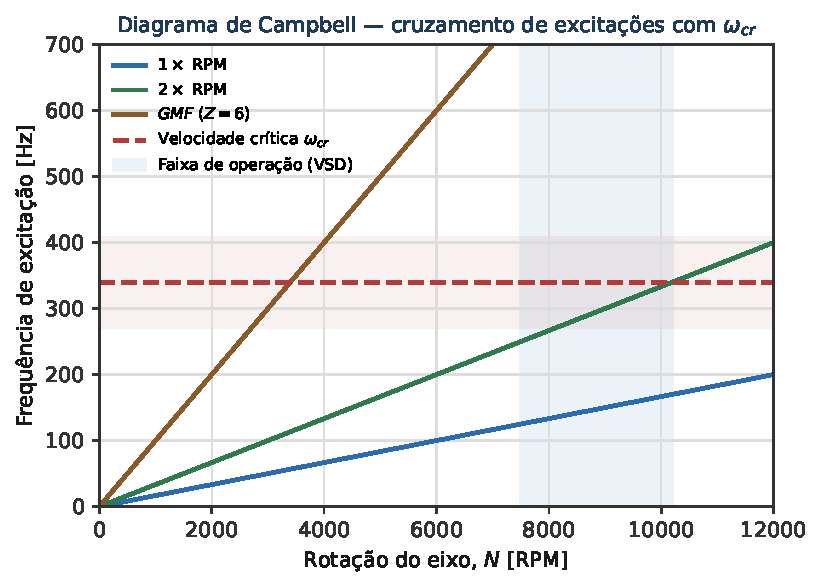
\includegraphics[width=0.75\textwidth]{figuras/fig_8_2_campbell.pdf}
		\caption[Diagrama de Campbell]{Diagrama de Campbell ilustrativo: cruzamento das linhas de excitação ($1\times$, $2\times$ RPM, GMF) com a velocidade crítica $\omega_{cr}$ e a faixa de operação do VSD.}
		\label{fig:8-2}
	\end{figure}

	\subsection{\textbf{Integridade dos Dentes e Modos de Falha de Engrenamento}}
	A saúde das engrenagens é avaliada através de modelos de fadiga de superfície e flexão.
	\begin{itemize}
		\item \textbf{Fadiga de Flexão (Tensão na Raiz - Lewis):} A Equação~\eqref{eq:s8-7} estima a tensão de flexão na base do dente da engrenagem — a força tangencial transmitida, dividida pela área efetiva da raiz do dente ($b \cdot m$) e pelo fator de forma de Lewis, e então ampliada por dois fatores de correção que penalizam efeitos dinâmicos ($K_v$) e distribuição desigual de carga ao longo da face ($K_m$):
		\begin{equation}\label{eq:s8-7}
 \sigma_b = \frac{W_t}{b \cdot m \cdot Y} \cdot K_v \cdot K_m
\end{equation}
		Onde $W_t$ é a força tangencial transmitida no dente, $b$ a largura de face da engrenagem, $m$ o módulo (geometria do dente), $Y$ é o fator de forma de Lewis, $K_v$ o fator dinâmico (velocidade de engrenamento) e $K_m$ o fator de distribuição de carga. A forma é a equação de flexão de Lewis, desenvolvida no capítulo de engrenagens cilíndricas e helicoidais de Shigley \cite[Cap.~14]{shigley}, com os fatores de correção na definição normalizada pela AGMA \cite{agma2001}. Uma trinca na raiz altera a rigidez, gerando impactos cíclicos no envelope de vibração.
		\item \textbf{Dano Adesivo (Scuffing):} O modelo calcula a Temperatura de Flash ($T_{\text{flash}}$) no contato instantâneo. Se $T_{\text{flash}} > T_{\text{crítica}}$, o sistema sinaliza falha iminente de lubrificação.
	\end{itemize}
	
	\subsection{\textbf{Desalinhamento e Arquiteturas de Acionamento}}
	\begin{itemize}
		\item \textbf{Desalinhamento:} Identificado por vibrações em $1 \times$ e $2 \times$ RPM (axial/radial). O desalinhamento interno eleva o fator $K_m$, concentrando tensões e reduzindo a vida útil das engrenagens.
		\item \textbf{Arquitetura Multi-Drive (Motores Independentes):} Elimina a \textit{gearbox} central, mas exige sincronismo eletrônico via VFD. A potência total é a soma individual, pela Equação~\eqref{eq:s8-8}:
		\begin{equation}\label{eq:s8-8}
 P_{\text{total}} = \sum \frac{\tau_i \cdot \omega_i}{\eta_{\text{mot},i}} 
\end{equation}
	\end{itemize}
	
	\subsection{\textbf{Matriz de Falhas de Transmissão}}
	A Tabela~\ref{tab:8-1} resume os principais modos de falha do trem de transmissão (rolamentos, dentes, sincronismo), suas causas raiz e o respectivo indicador digital de detecção.
	\begin{table}[h!tbp]
		\centering
		\small
		\renewcommand{\arraystretch}{1.5}
		\begin{tabular}{l l l}
			\toprule
			\textbf{Falha} & \textbf{Causa Raiz} & \textbf{Indicador Digital} \\ \midrule
			Desgaste de Rolamento & Fadiga / Contaminação & Picos em BPFO/BPFI e $\uparrow$ Curtose \\
			Pitting nos Dentes & Sobrecarga Cíclica & Bandas laterais na $GMF$ \\
			Quebra de Dente & Fadiga de Raiz (Lewis) & Impactos no envelope de vibração \\
			Desalinhamento & Montagem / Térmico & Vibração $2 \times \text{RPM}$ e $\uparrow K_m$ \\
			\textit{Scuffing} & Falha de Lubrificação & $\uparrow T$ de Flash e Partículas no Óleo \\
			Erro de Sincronismo & Desgaste \textit{Timing Gears} & Desvio de fase $\Delta \phi$ e oscilação de torque \\ \bottomrule
		\end{tabular}
		\caption[Matriz de falhas do trem de transmissão]{Matriz de falhas do trem de transmissão: rolamentos, dentes de engrenagem, alinhamento e sincronismo.}
		\label{tab:8-1}
	\end{table}
	
	\vspace{1em}
	\textbf{Condição de Estabilidade Mecânica:} A Equação~\eqref{eq:s8-9} resume, em duas desigualdades simultâneas, o critério de saúde de todo o trem de transmissão: a tensão real na raiz do dente (Equação~\eqref{eq:s8-7}) deve permanecer abaixo da tensão admissível do material, e o erro de fase entre os rotores de sincronismo deve permanecer menor que a folga de \textit{backlash} de projeto — a violação de qualquer uma indica risco iminente de quebra de dente ou contato metal-metal:
	\begin{equation}\label{eq:s8-9}
 \boxed{\sigma_{b, \text{real}} < \sigma_{b, \text{adm}} \quad \text{e} \quad \Delta \theta_{\text{sync}} < \theta_{\text{backlash}}}
\end{equation}

	\subsection{\textbf{Análise Torcional do Trem Completo}}
	A velocidade crítica $\omega_{cr}$ da Equação~\eqref{eq:s8-5} e a margem de separação da Equação~\eqref{eq:s8-6} tratam apenas do modo \textbf{lateral} de vibração do eixo — o rotor de Jeffcott flexiona transversalmente. Mas o conjunto motor–acoplamento–gearbox–rotores forma também um sistema massa-mola \textbf{torcional}, com seus próprios modos de ressonância em torção pura, independentes da rigidez lateral. Máquinas de alta potência exigem essa análise separadamente \cite{api684}: a rigidez torcional do eixo já calculada na Equação~\eqref{eq:s6-5} entra aqui como um dos elementos de um sistema de múltiplas inércias, não mais como um cálculo isolado de torção estática.

	Na aproximação de duas inércias — o rotor do motor ($I_1$) contra a inércia equivalente do trem de compressão referida ao eixo do motor ($I_2$, mesma referência já usada para $I_{\text{sys}}$ na Equação~\eqref{eq:s6-1}), conectadas pela rigidez torcional equivalente $k_{t,\text{eq}}$ (a associação em série da rigidez do eixo $k_t$ da Equação~\eqref{eq:s6-5} com a do acoplamento) — a frequência natural torcional fundamental é dada pela Equação~\eqref{eq:s8-10}:
	\begin{equation}\label{eq:s8-10}
 \omega_{cr,t} = \sqrt{k_{t,\text{eq}} \left( \frac{1}{I_1} + \frac{1}{I_2} \right)}
\end{equation}
	O critério de projeto exige a mesma lógica de margem de separação da Equação~\eqref{eq:s8-6}, mas contra um conjunto de excitações distinto: enquanto a ressonância lateral responde a $1\times$ RPM e $2\times$ RPM, a ressonância torcional é excitada também pela frequência de passagem de lóbulos ($f_{bp}$), pela frequência de engrenamento ($GMF$) e pelos harmônicos de torque gerados pelo chaveamento PWM do VSD (mesma origem física da distorção harmônica de corrente $\text{THD}_i$ já discutida no Capítulo de Subsistema Elétrico, agora manifestada como oscilação de torque em vez de corrente). Diferente da vibração lateral — que se manifesta como deslocamento radial detectável por acelerômetro — uma ressonância torcional pode não aparecer na carcaça: sua assinatura mais confiável é a oscilação cíclica do torque calculado, $\tau_{\text{ref}}$ da Equação~\eqref{eq:s6-8}, na frequência de $\omega_{cr,t}$.

	\vspace{1em}
	\hrule
	\vspace{1em}

	\textbf{Diretriz Técnica Final:} A Equação~\eqref{eq:s8-9} reúne as duas condições independentes de integridade do trem de transmissão — estrutural (fadiga do dente) e cinemática (sincronismo) — que devem ser satisfeitas simultaneamente; a violação de qualquer uma delas isoladamente já justifica a parada preventiva da máquina, mesmo que a outra permaneça dentro do limite. A Equação~\eqref{eq:s8-10} cobre um terceiro eixo de risco que nenhuma das duas anteriores captura: a ressonância torcional não quebra um dente nem desalinha o sincronismo diretamente, mas fadiga o próprio eixo e o acoplamento por ciclos de torque — e, ao contrário da vibração lateral já instrumentada no ponto B da Tabela~\ref{tab:18-1}, seu único sinal observável em campo costuma ser a oscilação do torque estimado, não uma leitura direta de sensor.

	% --- Fim do Capítulo 8 ---
	
	% --- Início do Capítulo 9: Termodinâmica do Estágio LP e Dinâmica de Folgas (Versão Integral) ---
	
	\clearpage
	\section{\textbf{Termodinâmica do Estágio LP, Dinâmica de Folgas e Resposta Vibracional}}
	\markboth{Termodinâmica do Estágio LP, Dinâmica de Folgas}{}

	Este capítulo detalha a física da compressão no primeiro estágio (LP), integrando a cinemática de engrenamento, o impacto das folgas micrométricas, o fenômeno de superaquecimento da carcaça e a assinatura vibracional resultante \cite{bently}. O modelo aqui descrito é a base para a detecção precoce de degradação nos rotores.
	
	\subsection{\textbf{Geometria de Engrenamento e Linha de Vedação}}
	O processo de compressão é definido pela variação volumétrica das câmaras formadas pela interação dos perfis dos rotores macho e fêmea.
	\begin{itemize}
		\item \textbf{Variação Volumétrica:} O volume $V$ é uma função do ângulo de rotação $\theta$. A taxa de variação temporal é dada pela Equação~\eqref{eq:s9-1}:
		\begin{equation}\label{eq:s9-1}
 \frac{dV}{dt} = \frac{dV}{d\theta} \cdot \omega 
\end{equation}
		\item \textbf{Área de Fuga Total ($A_{\text{leak}}$):} Representa a soma das passagens parasitas que permitem o retorno do gás entre câmaras de pressões distintas, pela Equação~\eqref{eq:s9-2}:
		\begin{equation}\label{eq:s9-2}
 A_{\text{leak}}(\theta) = L_{\text{seal}} \cdot \delta_f + L_{\text{tip}} \cdot \delta_r + A_{bh} 
\end{equation}
		Onde $L_{\text{seal}}$ é o comprimento da linha de vedação, $\delta_f$ a folga de flanco, $\delta_r$ a folga radial e $A_{bh}$ a área do triângulo de fuga (\textit{blow-hole}).
	\end{itemize}
	
	\subsection{\textbf{Dinâmica de Fugas e Razão de Pressão (\texorpdfstring{$\Pi$}{Pi})}}
	As folgas determinam a capacidade do estágio de sustentar a pressão e a eficiência volumétrica ($\eta_v$).
	\begin{itemize}
		\item \textbf{Eficiência Volumétrica e Folga:} O aumento da folga $\delta$ reduz a pressão efetiva de descarga $P_2$ para uma mesma rotação $\omega$, conforme a Equação~\eqref{eq:s9-3}:
		\begin{equation}\label{eq:s9-3}
 \eta_v = 1 - K \cdot \left( \frac{\delta}{L} \right) \cdot \sqrt{\frac{P_2}{P_1}} 
\end{equation}
		Onde $L$ é o comprimento de referência do rotor (normaliza a folga $\delta$) e $K$ é uma constante empírica de vazamento, calibrada por ensaio de desempenho da máquina (agrega efeitos de geometria do perfil e coeficiente de descarga não capturados explicitamente pelos demais termos). A Figura~\ref{fig:9-1} mostra que a queda de $\eta_v$ com o desgaste da folga é mais acentuada quanto maior a razão de pressão do estágio — ou seja, o mesmo desgaste físico penaliza proporcionalmente mais um estágio HP do que um estágio LP.

		\begin{figure}[h!tbp]
			\centering
			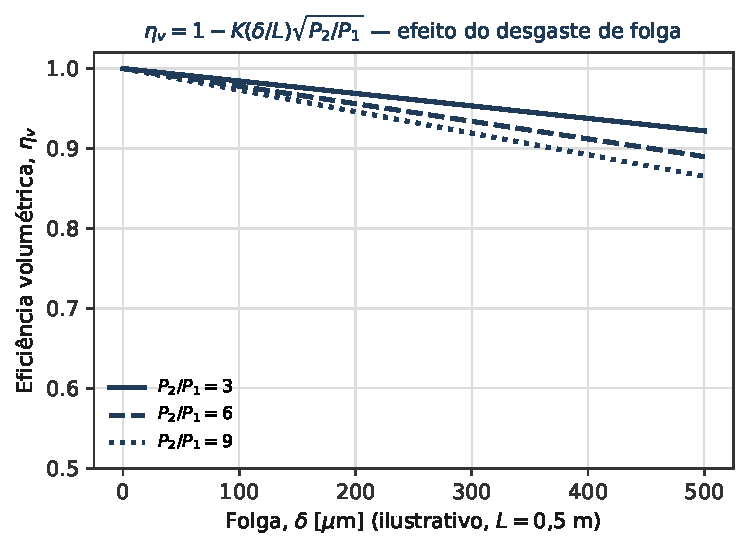
\includegraphics[width=0.60\textwidth]{figuras/fig_9_1_etav.pdf}
			\caption[Eficiência volumétrica em função da folga]{Eficiência volumétrica em função da folga do rotor, para diferentes razões de pressão do estágio.}
			\label{fig:9-1}
		\end{figure}
		\item \textbf{Fluxo de Massa de Fuga ($\dot{m}_{\text{leak}}$):} Modelado como escoamento compressível através de orifícios. O ar que retorna das câmaras de alta pressão reaquece o ar de sucção por pré-aquecimento (\textit{pre-heating}), pela Equação~\eqref{eq:s9-4}:
		\begin{equation}\label{eq:s9-4}
 T_{\text{suc,eff}} = \frac{\dot{m}_{\text{in}} T_{\text{in}} + \dot{m}_{\text{leak}} T_{\text{leak}}}{\dot{m}_{\text{in}} + \dot{m}_{\text{leak}}} 
\end{equation}
		\item \textbf{Índice Politrópico ($n$):} O desvio da compressão adiabática ideal é monitorado pelo índice $n$, definido na Equação~\eqref{eq:s9-5}:
		\begin{equation}\label{eq:s9-5}
 n = \frac{\ln(P_2/P_1)}{\ln(P_2/P_1) - \ln(T_2/T_1)} 
\end{equation}
	\end{itemize}
	
	\subsection{\textbf{Superaquecimento da Carcaça e Dilatação Térmica}}
	A carcaça atua como dissipador térmico. O superaquecimento altera as folgas críticas por dilatação diferencial entre estator e rotor.
	\begin{itemize}
		\item \textbf{Balanço Térmico da Carcaça:} A Equação~\eqref{eq:s9-6} descreve como a temperatura da carcaça ($T_c$) evolui no tempo: sua capacidade térmica (massa $M_c$ vezes calor específico $c_c$) acumula a diferença entre o calor gerado internamente pela compressão ($\dot{Q}_{\text{int}}$) e o calor que consegue escapar — por convecção externa ($\dot{Q}_{\text{ext}}$) e pelo sistema de arrefecimento ($\dot{Q}_{\text{arref}}$):
		\begin{equation}\label{eq:s9-6}
 M_c c_c \frac{dT_c}{dt} = \dot{Q}_{\text{int}} - \dot{Q}_{\text{ext}} - \dot{Q}_{\text{arref}}
\end{equation}
		\item \textbf{Folga Residual Real ($\delta_{\text{real}}$):} O Gêmeo Digital calcula a folga instantânea considerando a expansão térmica dos rotores ($r$) e da carcaça ($c$), pela Equação~\eqref{eq:s9-7}:
		\begin{equation}\label{eq:s9-7}
 \delta_{\text{real}} = \delta_{\text{nom}} - (\alpha_r L_r \Delta T_r - \alpha_c L_c \Delta T_c) 
\end{equation}
		Se $\delta_{\text{real}} \to 0$, o modelo sinaliza risco iminente de contato (\textit{rubbing}).
	\end{itemize}
	
	\subsection{\textbf{Acoplamento Fluido-Estrutural e Resposta Vibracional}}
	A alteração nas folgas e na pressão interna gera forças de excitação mecânica detectáveis no espectro de frequência.
	\begin{itemize}
		\item \textbf{Frequência de Passagem dos Lóbulos ($f_{bp}$):} Assinatura principal do engrenamento — cada vez que um lóbulo do rotor macho passa por uma posição fixa da carcaça, ele gera um pulso de pressão. A Equação~\eqref{eq:s9-8} calcula a frequência desses pulsos multiplicando a frequência de giro do rotor macho pelo seu número de lóbulos ($Z_{\text{macho}}$). Como a rotação $N_{\text{macho}}$ é medida em RPM e $f_{bp}$ é expressa em Hz, é obrigatória a divisão por 60 — a mesma conversão já formalizada na Equação~\eqref{eq:s6-7}, e a fonte de erro mais comum ao configurar a faixa de análise espectral do sistema de monitoramento:
		\begin{equation}\label{eq:s9-8}
 f_{bp} = \frac{N_{\text{macho}}}{60} \cdot Z_{\text{macho}} = f_{r,\text{macho}} \cdot Z_{\text{macho}}
\end{equation}
		\item \textbf{Diagnóstico Vibracional:}
		\begin{itemize}
			\item \textbf{Aumento de Folgas:} Reduz o amortecimento pneumático entre rotores, elevando a amplitude em $f_{bp}$ e gerando pulsações de pressão na descarga.
			\item \textbf{Desalinhamento Térmico:} O gradiente de temperatura na carcaça causa empenamento (\textit{casing distortion}), resultando em picos em $1 \times$ e $2 \times$ RPM e aumento da vibração axial.
			\item \textbf{Contato (\textit{Rubbing}):} Caracterizado por emissões acústicas de alta frequência, picos não-harmônicos e aumento do ruído de fundo (\textit{noise floor}).
		\end{itemize}
	\end{itemize}
	
	\subsection{\textbf{Potência Real e Eficiência Isentrópica}}
	A potência absorvida pelo estágio LP ($\dot{W}_{\text{LP}}$) integra as perdas por fuga e calor. A eficiência isentrópica $\eta_{is}$ é o principal KPI de saúde, na Equação~\eqref{eq:s9-9}:
	\begin{equation}\label{eq:s9-9}
 \dot{W}_{\text{LP}} = \frac{\dot{m} \cdot c_p \cdot T_1}{\eta_{is}} \left[ \left( \frac{P_2}{P_1} \right)^{\frac{\gamma - 1}{\gamma}} - 1 \right] 
\end{equation}
	
	\subsection{\textbf{Matriz de Falhas Integrada do Estágio LP}}
	A Tabela~\ref{tab:9-1} integra os modos de falha do estágio LP com seus indicadores digitais e a assinatura vibracional correspondente, permitindo diferenciar causas puramente térmicas de causas mecânicas.
	\begin{table}[h!tbp]
		\centering
		\renewcommand{\arraystretch}{1.5}
		\resizebox{\textwidth}{!}{
		\begin{tabular}{l l l l}
			\toprule
			\textbf{Falha} & \textbf{Causa Raiz} & \textbf{Indicador Digital} & \textbf{Resposta Vibracional} \\ \midrule
			Desgaste de Folgas & Erosão / Particulados & $\downarrow \Pi$ e $\downarrow \eta_v$ & $\uparrow$ Amplitude em $f_{bp}$ \\
			Superaquecimento & Falha Arrefecimento & $\uparrow T_c$ e $\uparrow T_2$ & $\uparrow$ Vibração Axial \\
			Contato (\textit{Rubbing}) & Dilatação Térmica & $\uparrow \uparrow T_2$ súbito & Picos HF / Emissão Acústica \\
			Perda de \textit{Coating} & Ciclos Térmicos & $\uparrow n$ (Politrópico) & $\uparrow$ Ruído de fundo \\
			Erosão do Perfil & Contaminação & $\uparrow A_{\text{leak}}$ calculado & Bandas laterais em $f_{bp}$ \\
			Desalinhamento & Falha Sincronismo & Oscilação de Torque & Picos em $1 \times$ e $2 \times$ RPM \\ \bottomrule
		\end{tabular}
		}
		\caption[Matriz de falhas integrada do estágio LP]{Matriz de falhas integrada do estágio LP: causa raiz, indicador digital e assinatura vibracional.}
		\label{tab:9-1}
	\end{table}
	
	\vspace{1em}
	\textbf{Condição de Alerta de Saúde do Estágio:} A Equação~\eqref{eq:s9-10} consolida os quatro sintomas discutidos neste capítulo — desvio na razão de pressão ($\Delta\Pi$), queda na eficiência isentrópica ($\Delta\eta_{is}$), aumento de vibração ($\Delta\text{Vib}$) e redução da folga residual ($\delta_{\text{real}}$) — em uma única função de saúde do estágio LP:
	\begin{equation}\label{eq:s9-10}
 \boxed{Health\_Index = f(\Delta \Pi, \Delta \eta_{is}, \Delta \text{Vib}, \delta_{\text{real}})}
\end{equation}

	\subsection{\textbf{Relação entre Eficiência Politrópica e Isentrópica}}
	Este capítulo usa $\eta_{is}$ (Equação~\eqref{eq:s9-9}) como KPI de saúde do estágio, e o índice politrópico $n$ (mesmo índice da Equação~\eqref{eq:s5-5}) como parâmetro do processo real de compressão — mas nunca a relação entre os dois. A distinção importa porque folhas de dados de fabricante de máquinas de alta potência frequentemente especificam a eficiência \textbf{politrópica} ($\eta_p$), não a isentrópica, e sem a conversão o Gêmeo Digital não consegue confrontar o modelo diretamente contra a garantia contratual do equipamento. A eficiência politrópica é definida a partir do próprio índice $n$ e do $\gamma$ do ar \cite{moran, cengel, hanlon}, pela Equação~\eqref{eq:s9-11}:
	\begin{equation}\label{eq:s9-11}
 \eta_p = \frac{\gamma - 1}{\gamma} \cdot \frac{n}{n - 1}, \qquad
 \eta_{is} = \frac{\Pi^{(\gamma-1)/\gamma} - 1}{\Pi^{(\gamma-1)/(\gamma\,\eta_p)} - 1}
\end{equation}
	A diferença física entre as duas eficiências é o que torna a Equação~\eqref{eq:s9-11} necessária, e não apenas uma curiosidade algébrica: $\eta_p$ é uma propriedade essencialmente \textbf{local} do processo de compressão (praticamente constante ao longo do mapa de operação da máquina, pois depende só de $n$ e $\gamma$), enquanto $\eta_{is}$ compara o processo real contra um caminho isentrópico fixo entre a mesma sucção e a mesma descarga — e por isso varia com a razão de pressão $\Pi$ mesmo que a máquina não tenha degradado nada. As duas eficiências não são intercambiáveis: um $\eta_{is}$ que cai ao operar em $\Pi$ mais alto não é, por si só, evidência de degradação — pode ser simplesmente a assinatura esperada de $\eta_p$ constante sob razão de pressão maior. O Gêmeo Digital deve monitorar $\eta_p$ (via Equação~\eqref{eq:s9-11}, invertida a partir de $n$ medido) como o indicador limpo de degradação real do estágio, e reservar $\eta_{is}$ para comparação direta com a garantia de fábrica na condição de projeto.

	\subsection{\textbf{Velocidade Periférica e Número de Mach na Ponta do Rotor}}
	As Equações~\eqref{eq:s9-2} e~\eqref{eq:s9-3} tratam a fuga através das folgas em função da geometria estática ($A_{\text{leak}}$) e da razão de pressão, mas nunca amarram esse escoamento à rotação do rotor — o parâmetro que efetivamente determina o regime do escoamento de fuga pela folga é a velocidade da própria superfície por onde o gás escapa. A velocidade periférica da ponta do rotor macho é dada pela Equação~\eqref{eq:s9-12}:
	\begin{equation}\label{eq:s9-12}
 u_{\text{tip}} = \frac{\pi \cdot D_{\text{macho}} \cdot N_{\text{macho}}}{60}
\end{equation}
	Onde $N_{\text{macho}}$ é a mesma rotação (RPM) do rotor macho já usada na Equação~\eqref{eq:s9-8} para a frequência de passagem de lóbulos, e o fator $60$ cumpre a mesma função de conversão para segundos. Comparando $u_{\text{tip}}$ com a velocidade do som local $a = \sqrt{\gamma R T}$ obtém-se o número de Mach na ponta, pela Equação~\eqref{eq:s9-13}:
	\begin{equation}\label{eq:s9-13}
 M_{\text{tip}} = \frac{u_{\text{tip}}}{a}
\end{equation}
	O papel de $M_{\text{tip}}$ é duplo. No vazamento pela folga (Equações~\eqref{eq:s9-2}--\eqref{eq:s9-3}), ele indica se o escoamento de fuga se aproxima do regime compressível/sônico — condição em que a vazão de fuga deixa de crescer proporcionalmente com $\Delta P$ e satura, alterando a forma esperada da própria Equação~\eqref{eq:s9-3}. No projeto do rotor, $M_{\text{tip}}$ é o limite físico que a geometria assimétrica de perfil precisa respeitar para manter a operação isenta de óleo estável e silenciosa \cite{fleming, hanlon} — velocidades de ponta elevadas demais aumentam perdas aerodinâmicas e ruído independentemente de qualquer degradação, de modo que um $M_{\text{tip}}$ crescente ao longo do tempo para a mesma rotação nominal é, em si, um sintoma a investigar (deriva de $D_{\text{macho}}$ efetivo por desgaste, ou erro de calibração de $T$ na estimativa de $a$).

	\subsection{\textbf{Fechamento do Balanço Térmico da Carcaça}}
	A Equação~\eqref{eq:s9-6} descreve como $T_c$ evolui no tempo, mas nenhum de seus três termos ($\dot{Q}_{\text{int}}$, $\dot{Q}_{\text{ext}}$, $\dot{Q}_{\text{arref}}$) foi, até aqui, expresso em função de grandezas já medidas ou já calculadas pelo Gêmeo Digital — a mesma lacuna que a Equação~\eqref{eq:s10-7} fechou para $P_{\text{sat}}(T)$ no capítulo seguinte. Fechar essa lacuna é o que permite estimar $T_c$ (e, por extensão, avaliar o risco de contato da Equação~\eqref{eq:s9-7}) mesmo em plantas offshore sem instrumentação dedicada de temperatura de carcaça.

	O calor gerado internamente é a perda mecânica de atrito (rotores e mancais) que não se converte em trabalho de compressão e permanece na máquina como calor. $\dot{W}_{\text{LP}}$ da Equação~\eqref{eq:s9-9} já está dividida por $\eta_{is}$ (perda termodinâmica do próprio processo de compressão), não por $\eta_{\text{mec}}$ — para chegar à potência de eixo real entregue pelo motor é preciso dividir novamente, agora por $\eta_{\text{mec}}$ (a mesma eficiência mecânica da Equação~\eqref{eq:s5-5}), e a perda mecânica é a diferença entre essa potência de eixo e $\dot{W}_{\text{LP}}$, pela Equação~\eqref{eq:s9-14}:
	\begin{equation}\label{eq:s9-14}
 \dot{Q}_{\text{int}} = \frac{\dot{W}_{\text{LP}}}{\eta_{\text{mec}}} - \dot{W}_{\text{LP}} = \dot{W}_{\text{LP}} \cdot \frac{1 - \eta_{\text{mec}}}{\eta_{\text{mec}}}
\end{equation}
	O calor que escapa da carcaça segue dois caminhos independentes, ambos regidos pela lei de Newton do resfriamento — proporcionais à diferença entre a temperatura da carcaça e a do ambiente ($T_c - T_{amb}$) — cada um com sua própria condutância térmica agregada: convecção natural pela superfície exposta da carcaça ($G_{\text{ext}}$) e o sistema de arrefecimento ativo do invólucro, tipicamente a ventilação forçada do \textit{hood} já descrita no Capítulo 2 ($G_{\text{arref}}$) — Equação~\eqref{eq:s9-15}:
	\begin{equation}\label{eq:s9-15}
 \dot{Q}_{\text{ext}} = G_{\text{ext}} \cdot (T_c - T_{amb}), \qquad
 \dot{Q}_{\text{arref}} = G_{\text{arref}} \cdot (T_c - T_{amb})
\end{equation}
	Substituindo as Equações~\eqref{eq:s9-14} e~\eqref{eq:s9-15} na Equação~\eqref{eq:s9-6} e resolvendo em regime permanente ($dT_c/dt=0$, a condição típica de operação estabilizada, sem evento transiente recente de carga), a temperatura de carcaça se torna uma função direta de grandezas já calculadas neste capítulo, pela Equação~\eqref{eq:s9-16}:
	\begin{equation}\label{eq:s9-16}
 T_{c} = T_{amb} + \frac{\dot{Q}_{\text{int}}}{G_{\text{ext}} + G_{\text{arref}}}
\end{equation}
	A rapidez com que a carcaça reage a uma mudança de carga (partida, alívio, evento de pico de demanda) é dada pela constante de tempo do sistema de primeira ordem definido pela linearização acima — razão entre a capacidade térmica da carcaça ($M_c$, $c_c$, já introduzidos na Equação~\eqref{eq:s9-6}) e a condutância total de dissipação — Equação~\eqref{eq:s9-17}:
	\begin{equation}\label{eq:s9-17}
 \tau_c = \frac{M_c \, c_c}{G_{\text{ext}} + G_{\text{arref}}}
\end{equation}
	Fora do regime permanente, a mesma linearização dá a solução transiente de primeira ordem $T_c(t) = T_{c} + (T_{c,0} - T_{c}) \cdot e^{-t/\tau_c}$, com $T_c$ da Equação~\eqref{eq:s9-16} e $T_{c,0}$ a condição inicial — a aproximação exponencial ao regime permanente após um degrau de $\dot{Q}_{\text{int}}$, forma idêntica à já usada para a resposta em rampa do inversor de frequência (Capítulo 13).

	Esse fechamento cobre apenas metade da Equação~\eqref{eq:s9-7}: a folga residual $\delta_{\text{real}}$ também depende da temperatura do próprio rotor ($T_r$), que a subseção a seguir fecha por um balanço térmico análogo ao de $T_c$.

	\subsection{\textbf{Fechamento da Temperatura do Rotor ($T_r$)}}
	O rotor não troca calor com o ambiente externo como a carcaça — ele é banhado internamente pelo próprio gás em compressão e perde calor por condução ao longo do eixo até os mancais, onde é finalmente dissipado pelo óleo de lubrificação. O balanço é estruturalmente idêntico ao da Equação~\eqref{eq:s9-6} (mesma forma de capacitância térmica acumulando a diferença entre geração e perda), mas com termos de troca próprios do rotor, pela Equação~\eqref{eq:s9-18}:
	\begin{equation}\label{eq:s9-18}
 M_r \, c_r \, \frac{dT_r}{dt} = h_r(\omega, \dot{m}) \cdot A_r \cdot (T_{\text{gas,med}} - T_r) - \dot{Q}_{\text{cond,eixo}}
\end{equation}
	Onde $M_r$ e $c_r$ são a massa e o calor específico do conjunto rotativo, $h_r$ o coeficiente de convecção gás-rotor (função da rotação $\omega$ e da vazão mássica $\dot{m}$, tipicamente correlações do tipo Nusselt-Reynolds para escoamento anular confinado), $A_r$ a área molhada do rotor, e $\dot{Q}_{\text{cond,eixo}}$ o calor conduzido pelo eixo para fora da câmara de compressão, em direção aos mancais. $T_{\text{gas,med}}$ é a temperatura média do gás que banha o rotor ao longo da compressão — aproximada pela média aritmética entre sucção e descarga do estágio, $T_{\text{gas,med}} \approx (T_{\text{in}} + T_{\text{out}})/2$, na ausência de um perfil de temperatura interno medido.

	Em regime permanente ($dT_r/dt = 0$), a mesma linearização usada na Equação~\eqref{eq:s9-16} para $T_c$ fecha $T_r$ diretamente, pela Equação~\eqref{eq:s9-19}:
	\begin{equation}\label{eq:s9-19}
 T_r = T_{\text{gas,med}} - \frac{\dot{Q}_{\text{cond,eixo}}}{h_r \cdot A_r}
\end{equation}
	Com $T_r$ e $T_c$ ambos calculáveis a partir do ponto de operação, a Equação~\eqref{eq:s9-7} deixa de depender de qualquer medição direta de temperatura interna — o Gêmeo Digital pode estimar a folga residual $\delta_{\text{real}}$ inteiramente a partir de grandezas já disponíveis (vazão, rotação, temperaturas de sucção/descarga), o mesmo valendo para a Equação~\eqref{eq:s11-7} do estágio HP. $h_r$ e $\dot{Q}_{\text{cond,eixo}}$ seguem como parâmetros de calibração específicos da máquina — assim como $G_{\text{ext}}$ e $G_{\text{arref}}$ o são para $T_c$ —, não valores de catálogo universais.

	\textbf{Ressalva sobre $T_{amb}$ em instalações com invólucro:} as Equações~\eqref{eq:s9-15}--\eqref{eq:s9-17} usam $T_{amb}$ como referência de convecção da carcaça, o que só é fisicamente correto para um compressor a céu aberto. Quando o elemento compressor está confinado no mesmo invólucro acústico que o motor, o VSD e a gearbox — arranjo comum em pacotes offshore por restrição de ruído, cobrindo às vezes o trem inteiro até a saída do 2º estágio (Capítulo 2) —, o ar que efetivamente banha a carcaça não é o ambiente externo, e sim o ar interno do invólucro, já aquecido pelas demais fontes de calor confinadas. Nesse caso, $T_{amb}$ nas três equações acima deve ser lido como $T_{\text{hood}}$, fechado pela Equação~\eqref{eq:s2-4} do Capítulo 2 — não como reescrita das equações (a forma matemática é idêntica), mas como reinterpretação do termo de referência. A ordem de cálculo correta está detalhada naquela seção.

	\vspace{1em}
	\hrule
	\vspace{1em}

	\textbf{Diretriz Técnica Final:} O Índice de Saúde da Equação~\eqref{eq:s9-10} só é interpretável se cada uma de suas quatro entradas ($\Pi$, $\eta_{is}$, vibração, $\delta_{\text{real}}$) for rastreada individualmente na Matriz de Falhas apresentada acima — reduzir tudo a um único número sem manter o detalhamento por causa raiz transforma um diagnóstico acionável em apenas mais um alarme genérico. A Equação~\eqref{eq:s9-11} adiciona a mesma cautela ao próprio $\Delta\eta_{is}$ que alimenta esse índice: antes de contar uma queda de $\eta_{is}$ como sintoma de falha, o Gêmeo Digital deve descontar a parcela que é apenas o efeito esperado de operar em razão de pressão distinta do ponto de garantia — só o resíduo depois desse desconto é degradação real. As Equações~\eqref{eq:s9-14}--\eqref{eq:s9-19} fecham o último elo puramente conceitual do capítulo: com elas, $T_c$ e $T_r$ deixam de ser grandezas que só sensores dedicados poderiam fornecer e passam a ser calculáveis a partir do próprio ponto de operação — mas a Equação~\eqref{eq:s9-17} também é um lembrete de escala: $\tau_c$ tipicamente responde em minutos a dezenas de minutos, ordem de grandeza muito maior que a dinâmica de pressão da rede (Capítulo 13) — um alarme de superaquecimento de carcaça nunca deve ser dimensionado com a mesma constante de tempo usada para a resposta do VSD.

	% --- Fim do Capítulo 9 ---
	
	% --- Início do Capítulo 10: Intercooler, Condensado e Distúrbios de Rede ---
	
	\clearpage
	\section{\textbf{Dinâmica do Intercooler, Gestão de Condensado e Distúrbios de Rede}}
	
	Este capítulo detalha a modelagem do resfriamento intermediário, integrando a termodinâmica de troca térmica, a psicrometria de condensação e a distinção entre falhas internas e distúrbios operacionais externos, como o impacto térmico de operações de sobrecarga de utilidade (\textit{offloading}).
	
	\subsection{\textbf{Termodinâmica de Troca Térmica e Efetividade}}
	O intercooler opera como um trocador de calor de correntes cruzadas ou contracorrente. A taxa de transferência de calor ($\dot{Q}$) é governada pelo balanço de energia e pela equação de transferência global, na Equação~\eqref{eq:s10-1}:

	\begin{equation}\label{eq:s10-1}
	\begin{aligned}
		\dot{Q} &= \dot{m}_a \cdot c_{p,a} \cdot (T_{LP,\text{out}} - T_{HP,\text{in}}) \\[4pt]
		\dot{Q} &= U \cdot A \cdot \Delta T_{lm} \cdot F
	\end{aligned}
\end{equation}
	
	Onde $\Delta T_{lm}$ é a Diferença de Temperatura Média Logarítmica (LMTD), forma fechada clássica para a força motriz térmica em trocadores de calor \cite{cengel, incropera}, dada pela Equação~\eqref{eq:s10-2}:

	\begin{equation}\label{eq:s10-2}
	\Delta T_{lm} = \frac{(T_{LP,\text{out}} - T_{w,\text{out}}) - (T_{HP,\text{in}} - T_{w,\text{in}})}{\ln \left( \frac{T_{LP,\text{out}} - T_{w,\text{out}}}{T_{HP,\text{in}} - T_{w,\text{in}}} \right)}
\end{equation}

	A origem física dessa expressão logarítmica fica clara ao observar o perfil de temperatura ao longo do trocador (Figura~\ref{fig:10-1}): como a diferença de temperatura entre os dois fluidos ($\Delta T_1$ na entrada, $\Delta T_2$ na saída) varia continuamente ao longo do comprimento, a força motriz térmica ``média'' correta não é a média aritmética simples, e sim a média logarítmica dessas duas diferenças extremas.

	\begin{figure}[h!tbp]
		\centering
		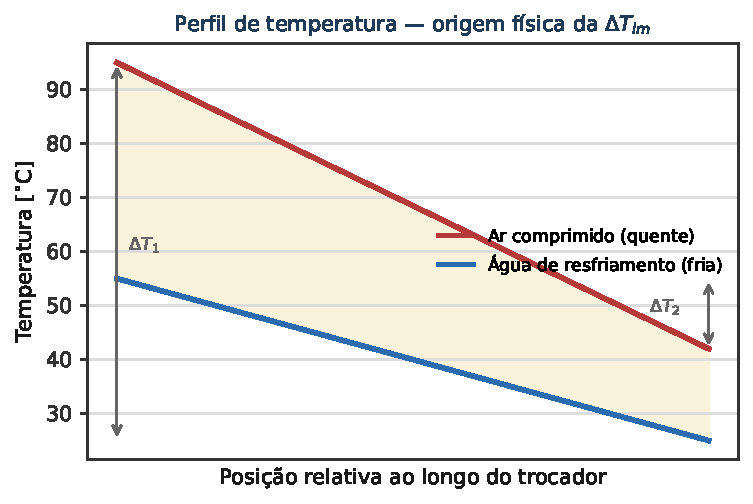
\includegraphics[width=0.60\textwidth]{figuras/fig_10_1_lmtd.pdf}
		\caption[Perfil de temperatura e origem física da LMTD]{Perfil de temperatura ao longo de um trocador em contracorrente — origem física da LMTD.}
		\label{fig:10-1}
	\end{figure}

	Para isolar a performance do ativo das flutuações da planta, o Gêmeo Digital monitora a Efetividade ($\epsilon$), pela Equação~\eqref{eq:s10-3}:

	\begin{equation}\label{eq:s10-3}
	\epsilon = \frac{T_{LP,\text{out}} - T_{HP,\text{in}}}{T_{LP,\text{out}} - T_{w,\text{in}}}
\end{equation}
	
	\subsection{\textbf{Mecanismo de Falha Externa: Sobrecarga Térmica (\textit{Offloading})}}
	Durante operações de \textit{offloading}, a temperatura da água de resfriamento ($T_{w,\text{in}}$) aumenta devido à demanda de outros consumidores. O Gêmeo Digital quantifica a penalidade de potência no estágio HP resultante deste distúrbio, pela Equação~\eqref{eq:s10-4}:

	\begin{equation}\label{eq:s10-4}
	\begin{aligned}
		\Delta \dot{W}_{\text{penalty}} &= \dot{W}_{HP}(T_{w,\text{in,atual}}) - \dot{W}_{HP}(T_{w,\text{in,nominal}}) \\[4pt]
		\dot{W}_{HP} &= \frac{\dot{m} \cdot R \cdot T_{HP,\text{in}}}{\eta_{is}} \cdot \left( \frac{\gamma}{\gamma-1} \right) \cdot \left[ \left( \frac{P_{HP,\text{out}}}{P_{HP,\text{in}}} \right)^{\frac{\gamma-1}{\gamma}} - 1 \right]
	\end{aligned}
\end{equation}
	
	\textbf{Diagnóstico:} Se $\epsilon$ permanece constante enquanto $T_{HP,\text{in}}$ e $\dot{W}_{HP}$ aumentam, o modelo classifica o evento como \textit{External Thermal Disturbance}.
	
	\subsection{\textbf{Mecanismo de Falha Interna: Incrustação (\textit{Fouling})}}
	A degradação interna é modelada pelo acúmulo de resistência térmica adicional ($R_f$). O coeficiente global de transferência real ($U_{\text{real}}$) é comparado ao valor de projeto ($U_{\text{clean}}$). A Equação~\eqref{eq:s10-5} nada mais é que a definição de resistência térmica global em série \cite[Cap.~11]{incropera}, escrita de modo que a incrustação apareça como uma resistência acrescentada ao caminho térmico limpo — e, na forma isolada à direita, como grandeza calculável a partir de medições de campo:
	
	\begin{equation}\label{eq:s10-5}
	\frac{1}{U_{\text{real}}} = \frac{1}{U_{\text{clean}}} + R_f \implies R_f = \frac{A \cdot \Delta T_{lm}}{\dot{Q}} - \frac{1}{U_{\text{clean}}}
\end{equation}
	
	O Gêmeo Digital utiliza a tendência de $R_f$ para prever a saturação térmica do trocador.
	
	\subsection{\textbf{Psicrometria e Extração de Condensado}}
	O resfriamento do ar comprimido frequentemente atinge o ponto de orvalho. A massa de água líquida gerada ($\dot{m}_{\text{cond}}$) é calculada pela variação da umidade específica ($W$ — convenção ASHRAE \cite{ashrae} para razão de umidade, evitando colisão com a velocidade angular $\omega$), pela Equação~\eqref{eq:s10-6}:

	\begin{equation}\label{eq:s10-6}
	\begin{aligned}
		W &= 0.622 \cdot \frac{\phi \cdot P_{\text{sat}}(T)}{P - \phi \cdot P_{\text{sat}}(T)} \\[4pt]
		\dot{m}_{\text{cond}} &= \dot{m}_a \cdot (W_{\text{in}} - W_{\text{out}})
	\end{aligned}
\end{equation}

	Até este ponto do documento, $P_{\text{sat}}(T)$ é referenciada como variável de processo, mas nunca definida como função constitutiva — o que impede o Gêmeo Digital de calculá-la a partir de $T$ medida. Para o intervalo de temperaturas típico do resfriamento de ar comprimido offshore ($0\,^{\circ}\text{C}$ a $80\,^{\circ}\text{C}$), a correlação de Arden Buck \cite{buck}, na Equação~\eqref{eq:s10-7}, oferece precisão adequada sem exigir tabelas de vapor:
	\begin{equation}\label{eq:s10-7}
 P_{\text{sat}}(T) = 0.61121 \, \exp\left[ \left( 18.678 - \frac{T}{234.5} \right) \left( \frac{T}{257.14 + T} \right) \right] \quad [\text{kPa}, \; T \text{ em } ^{\circ}\text{C}]
\end{equation}
	A Figura~\ref{fig:10-2} mostra essa correlação em escala logarítmica: a pressão de saturação praticamente dobra a cada 10-12$^{\circ}$C de aumento de temperatura, o que explica por que uma pequena falha de resfriamento no aftercooler tem efeito desproporcional na quantidade de água que chega ao secador PSA a jusante.

	\begin{figure}[h!tbp]
		\centering
		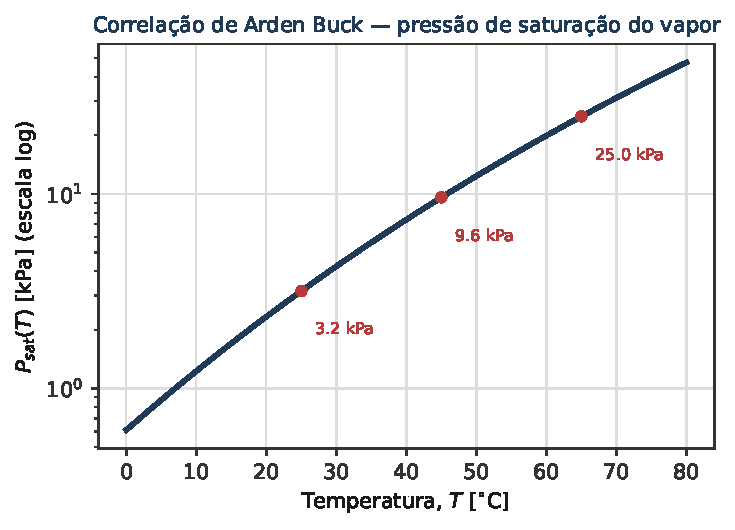
\includegraphics[width=0.60\textwidth]{figuras/fig_10_2_psat.pdf}
		\caption[Correlação de Arden Buck]{Correlação de Arden Buck para a pressão de saturação do vapor d'água em função da temperatura.}
		\label{fig:10-2}
	\end{figure}

	De forma análoga, o calor específico do ar úmido ($c_{p,\text{úmido}}$), usado implicitamente nas equações de $\dot{Q}$ e $\Delta T_{\text{oil}}$ ao longo deste capítulo, não é uma constante — ele deve incorporar a fração mássica de vapor d'água via $W$, pela Equação~\eqref{eq:s10-8}:
	\begin{equation}\label{eq:s10-8}
 c_{p,\text{úmido}} = c_{p,\text{ar seco}} + W \cdot c_{p,\text{vapor}} \approx 1005 + W \cdot 1860 \quad [\text{J}\,\text{kg}^{-1}\,\text{K}^{-1}] 
\end{equation}
	Ignorar essa correção introduz um viés sistemático nos balanços de energia dos trocadores em condições de alta umidade relativa offshore, justamente o cenário mais crítico para o dimensionamento do secador PSA a jusante. Mas $c_{p,\text{úmido}}$ só corrige a parcela \textbf{sensível} do balanço — a Equação~\eqref{eq:s10-1} continua incompleta enquanto tratar a troca térmica como puramente sensível, porque ignora o calor \textbf{latente} liberado pela própria condensação que a Equação~\eqref{eq:s10-6} calcula: cada quilograma de vapor que condensa libera sua entalpia de vaporização diretamente na água de resfriamento, não no ar. O balanço de energia total do trocador, incluindo essa parcela, fecha pela Equação~\eqref{eq:s10-9}:
	\begin{equation}\label{eq:s10-9}
	\begin{aligned}
		\dot{Q}_{\text{total}} &= \dot{m}_a \cdot c_{p,\text{úmido}} \cdot (T_{LP,\text{out}} - T_{HP,\text{in}}) + \dot{m}_{\text{cond}} \cdot h_{fg}(T_{HP,\text{in}}) \\[4pt]
		h_{fg}(T) &\approx 2\,501\,000 - 2360 \, T \quad [\text{J}\,\text{kg}^{-1}, \; T \text{ em } ^{\circ}\text{C}]
	\end{aligned}
\end{equation}
	$h_{fg}(T)$ é grafada em $\text{J}\,\text{kg}^{-1}$, não na forma mais comum em $\text{kJ}\,\text{kg}^{-1}$ ($\approx 2501 - 2{,}36\,T$) — essa é a mesma correlação, só reescrita nas unidades SI de $c_{p,\text{úmido}}$ (Equação~\eqref{eq:s10-8}), para que os dois termos da soma sejam diretamente compatíveis sem fator de conversão implícito. Em condições marinhas de alta umidade, essa parcela latente pode representar uma fração não desprezível de $\dot{Q}_{\text{total}}$ — omiti-la subestima a carga térmica real exigida da água de resfriamento e distorce tanto o cálculo de $U$ pela Equação~\eqref{eq:s10-5} (que usa $\dot{Q}$ no numerador de $R_f$) quanto qualquer dimensionamento derivado dele. A mesma correção se aplica ao aftercooler do Capítulo 14 (Equação~\eqref{eq:s14-2}), com $\dot{m}_{\text{cond}}$ da Equação~\eqref{eq:s14-3} no lugar da Equação~\eqref{eq:s10-6}.

	\textbf{Falha de Drenagem e Arraste:} A falha no sistema de purga resulta em acúmulo de líquido, identificado pelo aumento da perda de carga ($\Delta P_{\text{ar}}$) e pela assinatura vibracional de alta frequência no estágio HP — Equação~\eqref{eq:s10-10}:

	\begin{equation}\label{eq:s10-10}
	\Delta P_{\text{ar,real}} = f(\dot{m}_a, \rho) + \Delta P_{\text{obstrução}}
\end{equation}
	
	\subsection{\textbf{Matriz de Falhas Integrada do Sistema Intermediário}}

	A Tabela~\ref{tab:10-1} diferencia os distúrbios externos (\textit{offloading}, baixo fluxo de água) das falhas internas do próprio intercooler (\textit{fouling}, drenagem), cada um com sua variável de controle e ação recomendada.
	\begin{table}[h!tbp]
		\centering
		\renewcommand{\arraystretch}{1.5}
		\resizebox{\textwidth}{!}{
		\begin{tabular}{l l l l}
			\toprule
			\textbf{Mecanismo} & \textbf{Indicador Primário} & \textbf{Variável de Controle} & \textbf{Ação do Gêmeo} \\ \midrule
			\textit{Offloading} & $\uparrow T_{w,\text{in}}$ & $\epsilon \approx \text{constante}$ & Alerta de Rede Externa \\
			\textit{Fouling} & $\downarrow \epsilon$ e $\uparrow R_f$ & $U_{\text{real}} < U_{\text{limit}}$ & Sugestão de Limpeza \\
			Baixo Fluxo Água & $\uparrow \Delta T_{w}$ & $\downarrow \Delta P_{w}$ & Checar Bombas/Válvulas \\
			Falha Drenagem & $\uparrow \Delta P_{\text{ar}}$ & $\text{Vib}_{\text{HF,HP}} > \text{limit}$ & Alerta de Arraste/Erosão \\ \bottomrule
		\end{tabular}
		}
		\caption[Matriz de falhas do intercooler]{Matriz de falhas do intercooler: distúrbios externos versus falhas internas do trocador.}
		\label{tab:10-1}
	\end{table}
	
	\subsection{\textbf{Lógica de Predição de Trip e Saúde do Ativo}}
	O Índice de Saúde do Intercooler ($HI_{\text{IC}}$) e a predição de temperatura de descarga são calculados continuamente, pela Equação~\eqref{eq:s10-11}:

	\begin{equation}\label{eq:s10-11}
	\begin{cases}
		HI_{\text{IC}} = \omega_1 \cdot \left( \frac{\epsilon_{\text{real}}}{\epsilon_{\text{nom}}} \right) + \omega_2 \cdot \left( \frac{\Delta P_{\text{nom}}}{\Delta P_{\text{real}}} \right) \\[10pt]
		T_{HP,\text{out,pred}} = T_{HP,\text{in}} \cdot \Pi^{\frac{n-1}{n}}
	\end{cases}
\end{equation}
	
	Se $T_{HP,\text{out,pred}} \ge T_{\text{trip}}$, o Gêmeo Digital emite uma ordem de alívio de carga (\textit{load shedding}).

	\vspace{1em}
	\hrule
	\vspace{1em}

	\textbf{Diretriz Técnica Final:} A predição da Equação~\eqref{eq:s10-11} só tem valor preventivo se calculada com antecedência suficiente ao \textit{trip} — o Gêmeo Digital deve acionar o alívio de carga a partir da tendência projetada de $T_{HP,\text{out,pred}}$, não apenas quando o limite já tiver sido atingido pela medição real.

	% --- Fim do Capítulo 10 ---
	
	% --- Início do Capítulo 11: Estágio HP, Sincronismo e Integridade Mecânica ---
	
	\clearpage
	\section{\textbf{Estágio de Alta Pressão (HP), Sincronismo e Integridade Mecânica}}
	
	O estágio de Alta Pressão (HP) representa o maior desafio para o Gêmeo Digital, operando sob condições extremas de temperatura e pressão diferencial ($\Delta P$). Neste estágio, as folgas são reduzidas e qualquer desvio mecânico ou térmico pode resultar em falhas catastróficas. A Figura~\ref{fig:11-1} mostra o elemento compressor HP isolado da cadeia — mais compacto que o estágio LP da Figura~\ref{fig:2-3} pela razão já discutida no Capítulo de Arquitetura (maior pressão, menor vazão volumétrica) —, com a carcaça de mancais/engrenagens de sincronismo destacada, o coto de eixo com flange de acoplamento do lado de acionamento e os bocais de sucção (topo, vindo do intercooler) e descarga.

	\begin{figure}[h!tbp]
		\centering
		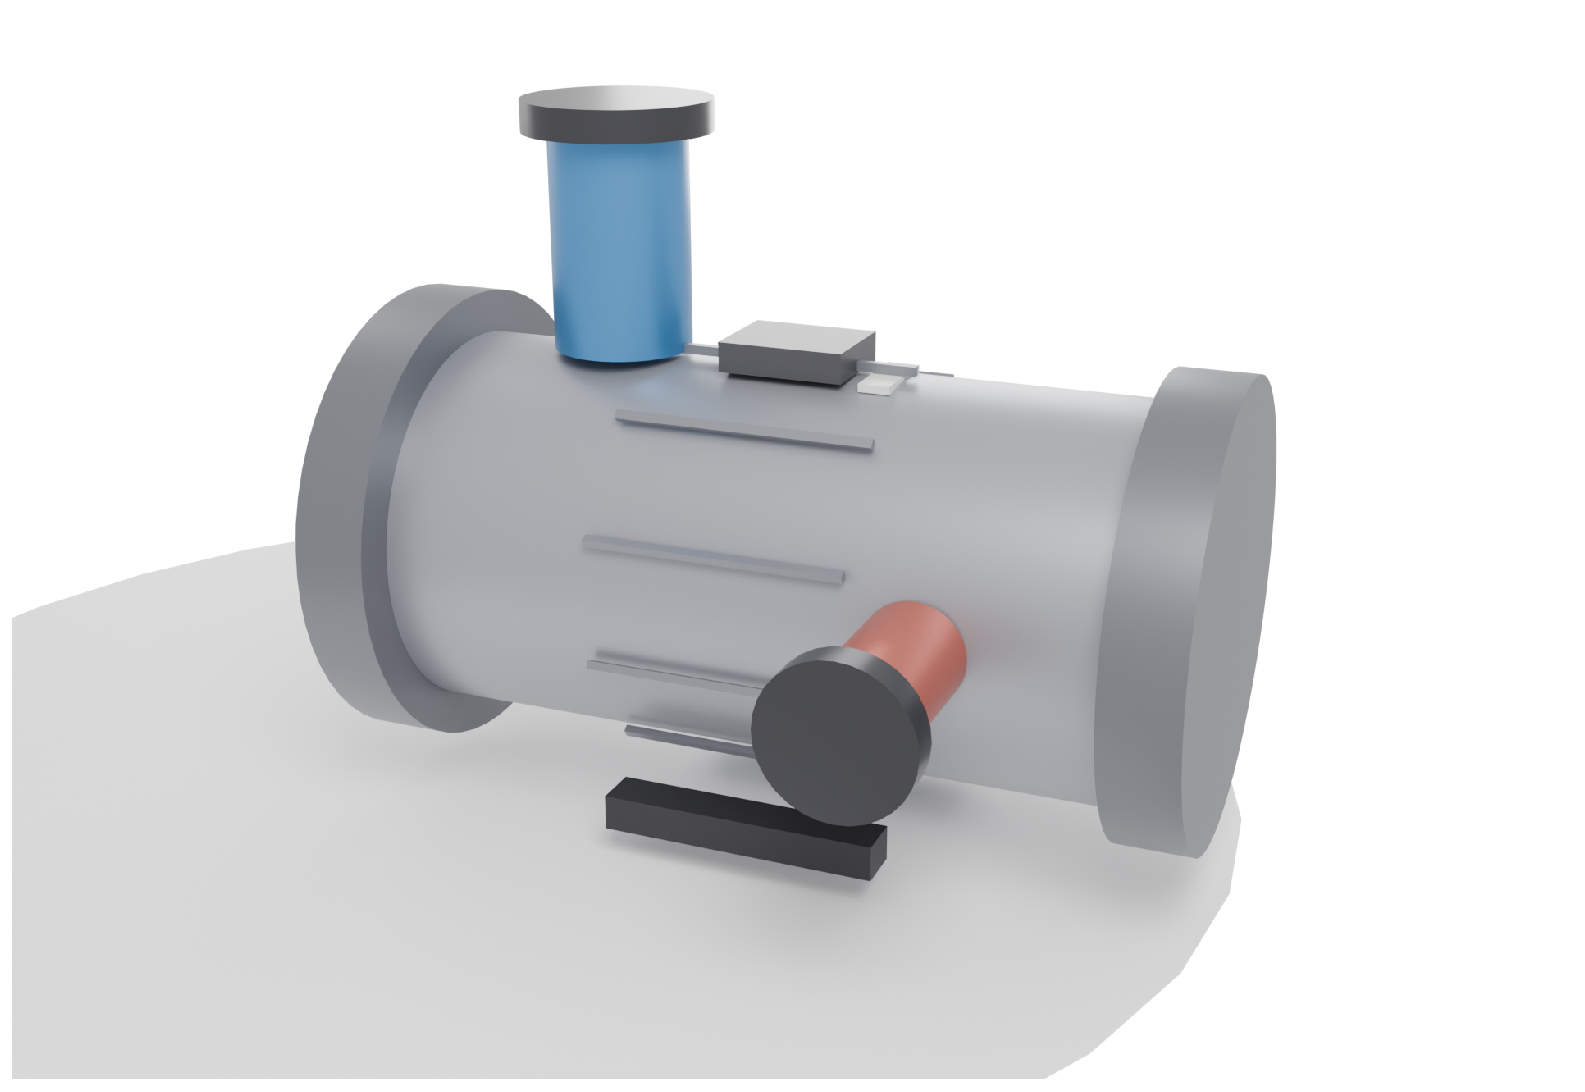
\includegraphics[width=0.75\textwidth]{figuras/fig_11_1_estagio_hp.pdf}
		\caption[Elemento compressor do estágio HP isolado]{Elemento compressor do estágio HP isolado, em perspectiva 3D — carcaça, mancais/engrenagens de sincronismo, coto de eixo e bocais de sucção/descarga. Esquema ilustrativo, não um desenho de projeto.}
		\label{fig:11-1}
	\end{figure}

	\subsection{\textbf{Termodinâmica e Performance do Estágio HP}}
	A compressão no estágio HP é modelada como um processo politrópico real, onde o índice $n$ reflete as perdas internas e a eficiência do resfriamento da carcaça. A Equação~\eqref{eq:s11-1} não é correlação empírica de fabricante: descende da expressão do trabalho de escoamento em processo internamente reversível, $w = \int v\,dP$, aplicada à relação politrópica $P v^{n} = \text{const.}$ — desenvolvimento clássico apresentado por Moran e colaboradores nos capítulos de entropia e de sistemas de potência a gás \cite[Cap.~6 e 9]{moran}. A Equação~\eqref{eq:s11-2} logo a seguir já não é politrópica — troca $n$ por $\gamma$ e divide por $\eta_{is}$, mesma formulação isentrópica-com-eficiência da Equação~\eqref{eq:s10-4} — mas soma às perdas termodinâmicas as perdas mecânicas de rolamentos e engrenagens de sincronismo, que a relação puramente politrópica de $T_{HP,\text{out}}$ não captura.
	
	\begin{itemize}
		\item \textbf{Temperatura de Descarga Final ($T_{HP,\text{out}}$):} Aplicando a relação politrópica de temperatura-pressão à razão de compressão do estágio HP, a Equação~\eqref{eq:s11-1} projeta a temperatura de descarga a partir da temperatura de sucção e da razão entre as pressões de saída e entrada, elevada ao expoente politrópico:
		\begin{equation}\label{eq:s11-1}
 T_{HP,\text{out}} = T_{HP,\text{in}} \cdot \left( \frac{P_{HP,\text{out}}}{P_{HP,\text{in}}} \right)^{\frac{n-1}{n}}
\end{equation}
		
		\item \textbf{Potência Total Absorvida ($\dot{W}_{HP,\text{tot}}$):}
		A potência integra o trabalho termodinâmico e as perdas mecânicas nos rolamentos e engrenagens de sincronismo, pela Equação~\eqref{eq:s11-2}:
		\begin{equation}\label{eq:s11-2}
 \dot{W}_{HP,\text{tot}} = \frac{\dot{m} \cdot R \cdot T_{HP,\text{in}}}{\eta_{is}} \left( \frac{\gamma}{\gamma-1} \right) \left[ \left( \frac{P_{HP,\text{out}}}{P_{HP,\text{in}}} \right)^{\frac{\gamma-1}{\gamma}} - 1 \right] + \dot{W}_{\text{fric,rol}} + \dot{W}_{\text{eng}} 
\end{equation}
		
		\item \textbf{Eficiência Volumétrica ($\eta_{v,HP}$):}
		É extremamente sensível às folgas internas ($\delta$) e à pressão diferencial. A forma da Equação~\eqref{eq:s11-3} vem de tratar cada folga como um \textbf{orifício de descarga}, mas o estágio HP opera sob razões de pressão altas o bastante para que a razão entre câmaras adjacentes ($r = P_{HP,\text{in}}/P_{HP,\text{out}}$) frequentemente caia abaixo da razão crítica $r_{cr} \approx 0{,}528$ (Equação~\eqref{eq:s13-2}) — a garganta da folga atinge regime sônico, e o modelo de orifício hidráulico incompressível ($\sqrt{2\rho\Delta P}$, sem limite superior à medida que $\Delta P$ cresce) superestima a vazão de fuga justamente na condição mais crítica de operação. A Equação~\eqref{eq:s11-3} reaproveita a mesma função de escoamento compressível $\Phi(r)$ da válvula de admissão (Equação~\eqref{eq:s13-1}), que satura corretamente no regime bloqueado:
		\begin{equation}\label{eq:s11-3}
 \eta_{v,HP} = 1 - \frac{\dot{m}_{\text{leak}}}{\dot{m}_{\text{th}}} = 1 - \frac{C_d \cdot A_{\text{gap}}(\delta) \cdot P_{HP,\text{out}} \cdot \sqrt{\dfrac{2}{R \cdot T_{HP,\text{out}}}} \cdot \Phi(r)}{\dot{m}_{\text{th}}}
\end{equation}
		Onde $C_d$ absorve a contração da veia fluida e o desvio em relação ao escoamento ideal, tal como na Equação~\eqref{eq:s13-1} — só que aqui a pressão e a temperatura a montante são as de descarga do próprio estágio HP ($P_{HP,\text{out}}$, $T_{HP,\text{out}}$), não as atmosféricas. No regime subsônico ($r > r_{cr}$), essa forma se reduz ao mesmo comportamento em raiz de $\Delta P$ já discutido — a fuga cresce com a \textit{raiz} da pressão diferencial, não linearmente. O tratamento de referência para desempenho de compressores de deslocamento positivo, com seção dedicada aos de parafuso, está no \textit{Compressor Handbook} \cite[Cap.~1 e 2]{hanlon}.
	\end{itemize}
	
	\subsection{\textbf{Dinâmica de Sincronismo e Cargas Mecânicas}}
	As engrenagens de sincronismo (\textit{timing gears}) e os rolamentos garantem a operação isenta de óleo (\textit{oil-free}) mantendo os rotores sem contato.
	
	\begin{itemize}
		\item \textbf{Engrenagens de Sincronismo:}
		O erro de transmissão e o \textit{backlash} ($\theta_b$) são monitorados para evitar o contato entre os lobos. O \textit{backlash} é a folga angular deliberadamente deixada entre os flancos dos dentes para acomodar dilatação térmica e o filme de lubrificante; seu crescimento por desgaste é o que degrada o sincronismo. A Equação~\eqref{eq:s11-4} expressa a folga de flanco residual como função dessa folga angular e do desgaste acumulado, sobre a mesma base de projeto de engrenagens que fornece a tensão de Lewis da Equação~\eqref{eq:s8-7} \cite[Cap.~13 e 14]{shigley}:
		\begin{equation}\label{eq:s11-4}
 \delta_{\text{flanco}} = f(\theta_b, \text{desgaste}) 
\end{equation}
		
		\item \textbf{Cargas nos Rolamentos de Escora (\textit{Thrust Bearings}):}
		O estágio HP gera um empuxo axial ($F_a$) massivo que deve ser equilibrado para evitar a colisão do rotor com a placa de descarga, pela Equação~\eqref{eq:s11-5}:
		\begin{equation}\label{eq:s11-5}
 F_a = (P_{HP,\text{out}} - P_{HP,\text{in}}) \cdot A_{\text{rotor}}
\end{equation}
		A Equação~\eqref{eq:s11-5} é um modelo — o sensor que fecha a malha entre esse modelo e a realidade física do mancal de escora é a sonda de proximidade de \textbf{posição axial} ($\delta_{ax}$), instrumentação de proximidade cuja prática a própria API 619 \cite{api619} referencia para máquinas desta classe de potência. O motivo de instrumentar posição, e não apenas vibração, é temporal: o desgaste do rolamento de escora se manifesta primeiro como uma deriva lenta e progressiva de $\delta_{ax}$ (o rotor ``caminha'' axialmente à medida que as pistas desgastam), muito antes de qualquer excitação vibratória mensurável aparecer — por isso $\delta_{ax}$ funciona como indicador de condição precoce para o mesmo modo de falha que a Equação~\eqref{eq:s11-6} projeta em horas restantes de vida.

		\item \textbf{Vida Útil Remanescente ($L_{10h}$):} Mesma formulação da vida nominal de rolamento apresentada na Equação~\eqref{eq:s8-4}, agora aplicada à carga axial equivalente do estágio HP ($P_{eq}$) e à rotação do eixo do estágio HP ($N_{\text{rot,HP}}$) — a Equação~\eqref{eq:s11-6} projeta as horas restantes de operação do rolamento de escora antes da falha por fadiga:
		\begin{equation}\label{eq:s11-6}
 L_{10h} = \left( \frac{C}{P_{eq}} \right)^p \cdot \frac{10^6}{60 \cdot N_{\text{rot,HP}}}
\end{equation}
		A rotação entra aqui em RPM, como em toda a família de equações de vida de rolamento deste documento — o fator $60$ do denominador é justamente a conversão para horas, e substituí-la pela velocidade angular $\omega$ (rad\,s$^{-1}$) produziria um resultado sem significado dimensional.
	\end{itemize}
	
	\subsection{\textbf{Mecanismos de Falha Detalhados}}
	
	\begin{enumerate}
		\item \textbf{Dilatação Térmica Diferencial e \textit{Rubbing}:}
		O aumento de $T_{w,\text{in}}$ (\textit{offloading}) eleva $T_{HP,\text{in}}$. A expansão térmica do rotor excede a da carcaça. A folga residual é dada pela Equação~\eqref{eq:s11-7}:
		\begin{equation}\label{eq:s11-7}
 \delta_{\text{res}} = \delta_{\text{nom}} - \alpha \cdot L \cdot (T_{\text{rotor}} - T_{\text{carcaça}}) 
\end{equation}
		Se $\delta_{\text{res}} \le 0$, ocorre contato metálico, detectado por picos de vibração e queda súbita de $\eta_{is}$. $T_{\text{rotor}}$ e $T_{\text{carcaça}}$ não precisam mais ser medidos ou estimados isoladamente para o estágio HP: são as mesmas Equações~\eqref{eq:s9-19} e~\eqref{eq:s9-16} do Capítulo 9, com $T_{\text{gas,med}}$ e $T_c$ recalculados a partir do ponto de operação do estágio HP.

		\item \textbf{Desgaste de Engrenagens e Perda de Sincronismo:}
		Causado por fadiga ou falha de lubrificação. O sintoma é o aumento dos harmônicos da frequência de engrenamento — Equação~\eqref{eq:s11-8}, mesma definição cinemática já usada no Capítulo de Engenharia do Trem de Transmissão — e alteração na fase vibracional entre os eixos:
		\begin{equation}\label{eq:s11-8}
 f_{gmf} = Z \cdot f_{\text{rot}}
\end{equation}
		
		\item \textbf{Falha de Selagem e \textit{Blow-by}:}
		Degradação dos selos de labirinto ou anéis de carvão. O Gêmeo Digital monitora o aumento da pressão no cárter ($P_{\text{cárter}}$) e a redução da vazão mássica efetiva.
		
		\item \textbf{Calço Hidráulico por Arraste de Condensado:}
		Falha no dreno do intercooler. O líquido incompressível gera um pico de torque instantâneo ($\Delta \tau$), pela Equação~\eqref{eq:s11-9}:
		\begin{equation}\label{eq:s11-9}
 \Delta \tau = I \cdot \frac{d\omega}{dt} + \tau_{\text{impacto}}
\end{equation}
		Resulta em quebra de dentes de engrenagens ou cisalhamento de chavetas.
		
		\item \textbf{Degradação do Revestimento (\textit{Coating}):}
		Erosão ou alta temperatura causam o aumento progressivo do índice politrópico $n$ e do Consumo de Potência Específica ($SPC$).
	\end{enumerate}
	
	\subsection{\textbf{Matriz de Diagnóstico do Estágio HP}}

	A Tabela~\ref{tab:11-1} resume os cinco modos de falha críticos do estágio HP e seu impacto relativo no Consumo de Potência Específica (SPC), permitindo priorizar a resposta do Gêmeo Digital.
	\begin{table}[h!tbp]
		\centering
		\small
		\renewcommand{\arraystretch}{1.5}
		\begin{tabular}{l l l c}
			\toprule
			\textbf{Falha} & \textbf{Indicador Primário} & \textbf{Variável de Controle} & \textbf{Impacto SPC} \\ \midrule
			\textit{Rubbing} Térmico & $\uparrow$ Vibração Global & $T_{HP,\text{out}} > T_{\text{limit}}$ & $\uparrow \uparrow$ \\
			Desgaste \textit{Gears} & $\uparrow$ Harmônicos $f_{gmf}$ & Erro de Fase & $\uparrow$ \\
			Fadiga Rolamento & $\uparrow T_{\text{mancal}}$ & $L_{10h} \to 0$ & $\uparrow$ \\
			Vazamento Selos & $\uparrow P_{\text{cárter}}$ & $\downarrow \eta_{v,HP}$ & $\uparrow \uparrow$ \\
			Arraste Líquido & $\uparrow$ Emissão Acústica & Picos de Torque $\Delta \tau$ & Crítico \\ \bottomrule
		\end{tabular}
		\caption[Matriz de diagnóstico do estágio HP]{Matriz de diagnóstico do estágio HP e impacto relativo de cada falha no SPC.}
		\label{tab:11-1}
	\end{table}
	
	\subsection{\textbf{Indicador de Saúde Global e KPI Final}}
	O Gêmeo Digital consolida os desvios no Índice de Saúde ($HI_{HP}$), pela Equação~\eqref{eq:s11-10}:
	\begin{equation}\label{eq:s11-10}
 HI_{HP} = w_1 \left( \frac{\eta_{v,\text{real}}}{\eta_{v,\text{nom}}} \right) + w_2 \left( \frac{T_{\text{out,nom}}}{T_{\text{out,real}}} \right) + w_3 \left( \frac{V_{\text{nom}}}{V_{\text{real}}} \right) 
\end{equation}
	
	O Consumo de Potência Específica ($SPC$) é o KPI final, na Equação~\eqref{eq:s11-11}:
	\begin{equation}\label{eq:s11-11}
 \boxed{SPC = \frac{\dot{W}_{LP,\text{tot}} + \dot{W}_{HP,\text{tot}}}{\dot{V}_{\text{free\_air}}}} 
\end{equation}
	Unidade: $\text{kW} \cdotp \text{m}^{-3} \cdotp \text{min}$.

	O denominador da Equação~\eqref{eq:s11-11}, $\dot{V}_{\text{free\_air}}$, não é a vazão volumétrica lida em qualquer condição de linha — é a vazão mássica medida $\dot{m}$, convertida às condições de referência de admissão padronizadas pela ISO 1217:2009/Amd 1:2016 \cite{iso1217} (a mesma norma já citada no Capítulo 1 para $\eta_{is}$): pressão absoluta $P_{\text{ref}} = 1\,\text{bar}$, temperatura $T_{\text{ref}} = 20\,^{\circ}\text{C}$ e umidade relativa nula. A Equação~\eqref{eq:s11-12} formaliza essa conversão:
	\begin{equation}\label{eq:s11-12}
 \dot{V}_{\text{free\_air}} = \frac{\dot{m}}{\rho_{\text{ref}}}, \qquad \rho_{\text{ref}} = \frac{P_{\text{ref}}}{R \cdot T_{\text{ref}}}
\end{equation}
	É essa normalização — não a vazão bruta de um instrumento de campo qualquer — que torna o $SPC$ comparável entre um dia quente e um frio, entre plataformas com pressão atmosférica local distinta, e contra a folha de dados do fabricante, que reporta o FAD nominal exatamente nessas mesmas condições de referência.

	\vspace{1em}
	\hrule
	\vspace{1em}

	\textbf{Diretriz Técnica Final:} O SPC da Equação~\eqref{eq:s11-11} é o KPI comercial que a operação enxerga, mas sua causa raiz — quando se degrada — está quase sempre em um dos termos do Índice de Saúde da Equação~\eqref{eq:s11-10}; o Gêmeo Digital deve sempre apresentar os dois juntos, nunca o SPC isolado sem a decomposição por componente.

	% --- Fim do Capítulo 11 ---
	
	% --- Início do Capítulo 12: Sistema de Lubrificação e Gestão Térmica ---
	
	\clearpage
	\section{\textbf{Sistema de Lubrificação e Gestão Térmica}}

	Este capítulo revisita o circuito de óleo já introduzido no Capítulo de Trem de Potência e detalhado no Capítulo de Sistema de Lubrificação, agora sob a ótica específica da gestão térmica do conjunto gearbox/mancais em condições de carga do estágio HP. Como o compressor deste documento é isento de óleo na câmara de compressão (nenhum óleo entra em contato com o ar de processo — ver Capítulo de Arquitetura), o papel do óleo aqui é exclusivamente remover o calor gerado por atrito na caixa multiplicadora e nos mancais e devolvê-lo já resfriado ao circuito; o Gêmeo Digital monitora esse balanço térmico e a integridade do elemento deaerador em tempo real. A Figura~\ref{fig:12-1} apresenta o trajeto físico completo do óleo — do reservatório à bomba, ao deaerador, à válvula termostática de três vias (que reparte a vazão entre o ramal do resfriador e o \textit{bypass} direto, Equação~\eqref{eq:s12-6}), até os mancais/gearbox, com a linha de retorno de volta ao reservatório em cor distinta.

	\begin{figure}[h!tbp]
		\centering
		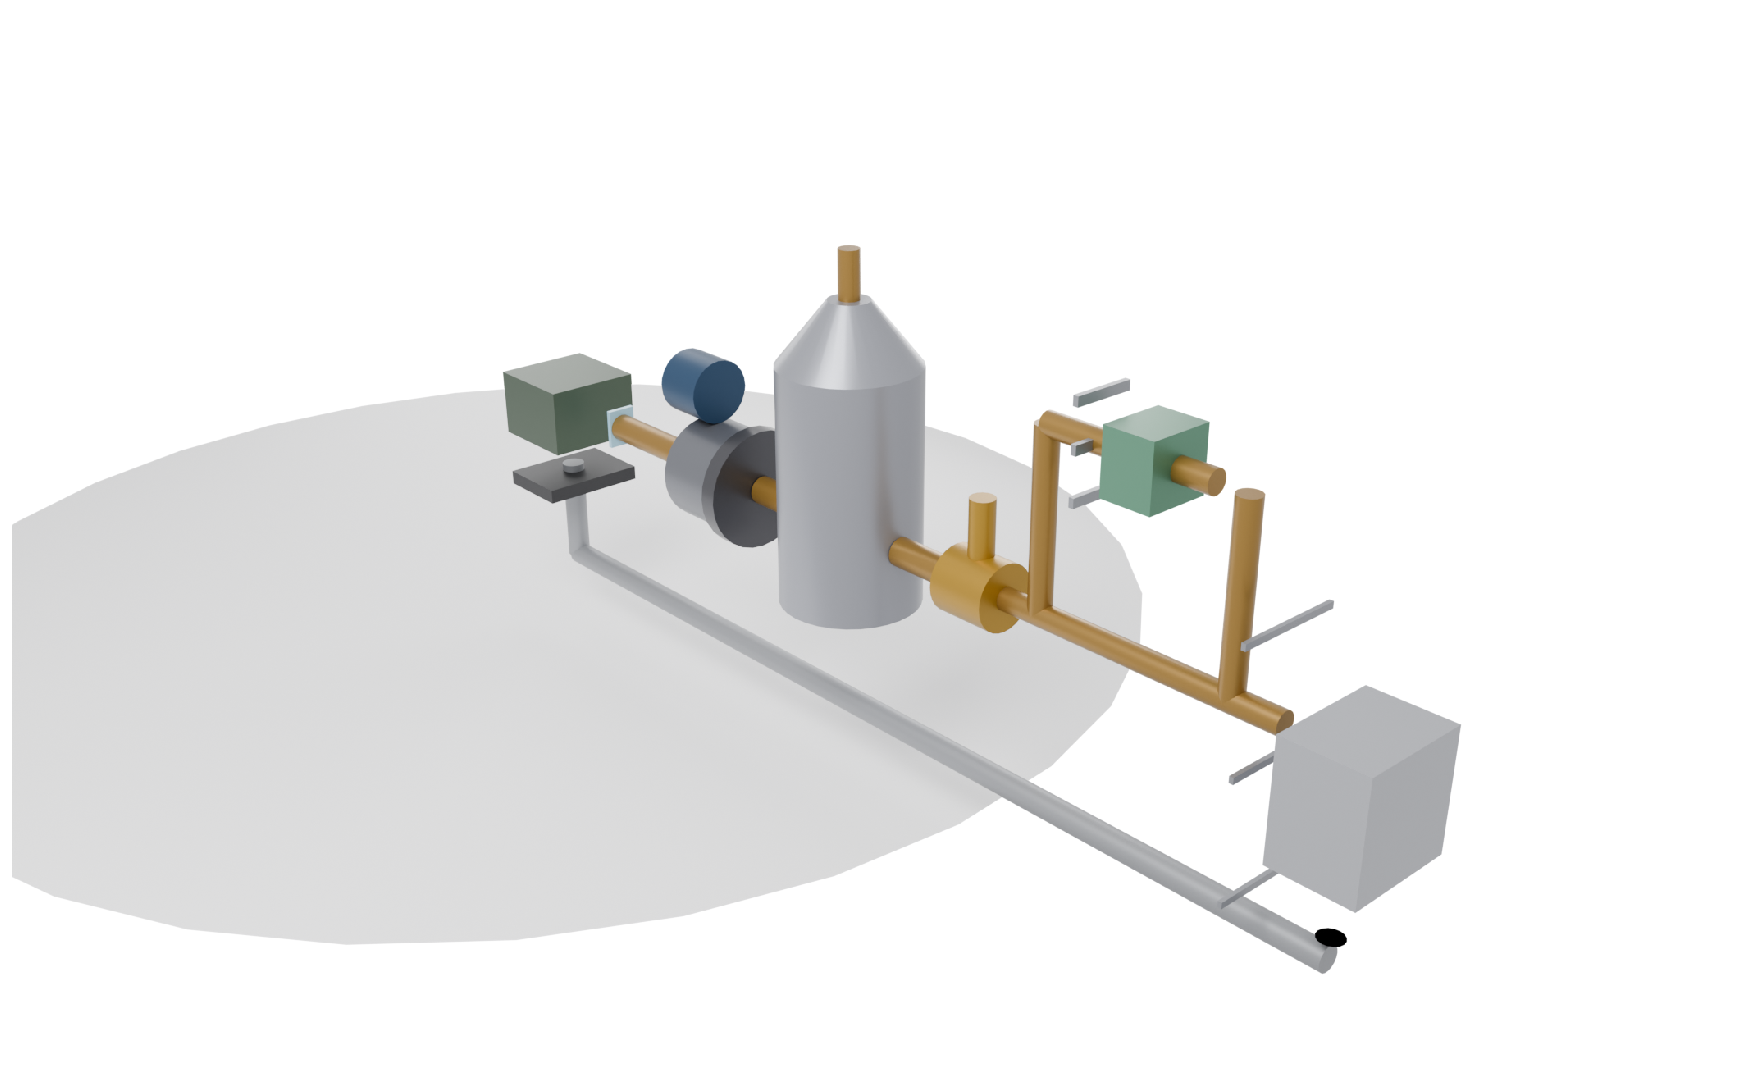
\includegraphics[width=0.80\textwidth]{figuras/fig_12_1_circuito_oleo.pdf}
		\caption[Circuito de óleo de lubrificação e arrefecimento]{Circuito de óleo de lubrificação e arrefecimento, em perspectiva 3D — reservatório, bomba, deaerador, válvula termostática de três vias, resfriador de óleo e retorno aos mancais/gearbox. Esquema ilustrativo, não um desenho de projeto.}
		\label{fig:12-1}
	\end{figure}

	\subsection{\textbf{Balanço de Energia do Circuito de Óleo}}
	A taxa de calor que o óleo remove do conjunto gearbox/mancais ($\dot{Q}_{\text{óleo}}$) é a mesma potência de atrito dissipada nesses componentes (Equações~\eqref{eq:s6-3}, \eqref{eq:s6-4} e \eqref{eq:s7-4}) — é fundamental mantê-la dentro da capacidade do resfriador para não elevar a temperatura de operação dos mancais além do limite do lubrificante — Equação~\eqref{eq:s12-1}:
	\begin{equation}\label{eq:s12-1}
 \dot{Q}_{\text{óleo}} = \dot{m}_{\text{óleo}} \cdotp c_{p,\text{óleo}} \cdotp (T_{\text{óleo,ret}} - T_{\text{óleo,sup}})
\end{equation}
	Onde $\dot{m}_{\text{óleo}}$ é a vazão mássica de óleo, $T_{\text{óleo,ret}}$ é a temperatura de retorno do óleo (já aquecido, saindo da gearbox/mancais) e $T_{\text{óleo,sup}}$ é a temperatura de suprimento após passar pelo resfriador de óleo — a mesma elevação de temperatura já modelada pelo balanço térmico do Capítulo de Sistema de Lubrificação (Equação~\eqref{eq:s7-5}), aqui reorganizada para isolar $\dot{Q}_{\text{óleo}}$ como a grandeza monitorada.

	\subsection{\textbf{Perda de Carga no Deaerador e Pressão de Suprimento aos Mancais}}
	Antes de alimentar os mancais e o engrenamento, o óleo de retorno passa por um separador de ar (deaerador) que libera as bolhas de ar incorporadas por respingo/turbulência durante a lubrificação — óleo aerado não sustenta o filme lubrificante nem dissipa calor com a mesma eficácia (ver Capítulo de Detalhamento de Componentes). A perda de carga nesse elemento ($\Delta P_{\text{sep}}$) cresce com a saturação e o tempo de uso; o modelo prevê a pressão que efetivamente chega aos mancais subtraindo essa perda da pressão de descarga da bomba de óleo ($P_{\text{bomba}}$, mantida pela bomba através da pressão $\Delta P_{\text{óleo}}$ já introduzida na Equação~\eqref{eq:s5-3}), pela Equação~\eqref{eq:s12-2}:
	\begin{equation}\label{eq:s12-2}
 P_{\text{sup,óleo}} = P_{\text{bomba}} - \Delta P_{\text{sep}}
\end{equation}
	Onde $\Delta P_{\text{sep}}$ é modelado em função da vazão volumétrica e da viscosidade cinemática do óleo $\nu(T)$. Uma queda de $P_{\text{sup,óleo}}$ abaixo do mínimo de projeto arrisca lubrificação insuficiente do engrenamento e dos mancais, mesmo que a vazão de óleo na saída da bomba esteja nominal.

	\subsection{\textbf{Capacidade do Resfriador: por que a Efetividade Não Basta}}
	O Capítulo 7 introduziu a efetividade $\epsilon$ (Equação~\eqref{eq:s7-6}) como indicador de saúde do resfriador de óleo, e ela cumpre bem esse papel enquanto as condições de contorno permanecem estáveis. Sob a carga do estágio HP em uma unidade offshore, porém, elas não permanecem estáveis: a temperatura de entrada da água de resfriamento acompanha a temperatura do mar e a carga dos demais consumidores do circuito de água, e a vazão disponível varia com a abertura de válvulas compartilhadas com outros equipamentos da planta. O problema é que $\epsilon$ responde a essas variações externas exatamente como responderia a uma incrustação interna — cai nos dois casos. Um alarme baseado apenas em $\epsilon$ é, portanto, ambíguo: ele não distingue ``o trocador sujou'' de ``a água de resfriamento chegou mais quente ou mais devagar''.

	A saída é monitorar a grandeza que descreve o trocador \textbf{independentemente} das temperaturas de entrada: a condutância térmica global $UA$ (produto do coeficiente global de transferência pela área de troca). Ela é obtida diretamente do calor efetivamente removido — já conhecido pela Equação~\eqref{eq:s12-1} — dividido pela diferença de temperatura média logarítmica entre óleo e água, pela Equação~\eqref{eq:s12-3}:
	\begin{equation}\label{eq:s12-3}
	UA_{\text{real}} = \frac{\dot{Q}_{\text{óleo}}}{\Delta T_{lm}}
	\end{equation}
	Onde $\Delta T_{lm}$ é a mesma LMTD já definida no Capítulo 10 para o intercooler, aqui aplicada ao par óleo/água. O ponto prático é que a Equação~\eqref{eq:s12-3} não exige instrumentação nova: as quatro temperaturas (entrada e saída de óleo, entrada e saída de água) e a vazão de óleo já são necessárias para o balanço da Equação~\eqref{eq:s12-1}.

	A relação entre as duas grandezas passa pelo número de unidades de transferência $NTU$ e pela razão de capacidades térmicas $C_r$, onde $C = \dot{m} \cdot c_p$ é a capacidade térmica de cada corrente. Para um trocador em contracorrente, a efetividade é uma função fechada dessas duas quantidades \cite{incropera}, conforme a Equação~\eqref{eq:s12-4}:
	\begin{equation}\label{eq:s12-4}
	\epsilon = \frac{1 - \exp\left[-NTU\,(1 - C_r)\right]}{1 - C_r \cdot \exp\left[-NTU\,(1 - C_r)\right]}, \qquad NTU = \frac{UA}{C_{\min}}, \qquad C_r = \frac{C_{\min}}{C_{\max}}
	\end{equation}
	A leitura diagnóstica da Equação~\eqref{eq:s12-4} é o que interessa ao Gêmeo Digital. A efetividade depende de $UA$, mas também de $C_{\min}$ — ou seja, das vazões. Uma redução na vazão de água de resfriamento derruba $\epsilon$ sem alterar em nada o estado físico do trocador. Já $UA$ só cai quando a superfície de troca de fato degrada: incrustação nos tubos, bolsão de ar retido no casco, tubos obstruídos ou vazamento interno. Normalizando pelo valor de projeto obtém-se um indicador adimensional de degradação, análogo à resistência de incrustação $R_f$ usada para o intercooler na Equação~\eqref{eq:s10-5}, mas expresso como fração da capacidade original — Equação~\eqref{eq:s12-5}:
	\begin{equation}\label{eq:s12-5}
	\eta_{UA} = \frac{UA_{\text{real}}}{UA_{\text{projeto}}}
	\end{equation}
	Um $\eta_{UA}$ estável com $\epsilon$ em queda aponta para fora da máquina — utilidade de água de resfriamento. Um $\eta_{UA}$ em queda sustentada aponta para dentro do trocador, e é ele, não $\epsilon$, que deve disparar a ordem de limpeza.

	\subsection{\textbf{Válvula Termostática e Temperatura de Suprimento}}
	A lógica da válvula termostática de três vias foi descrita qualitativamente no Capítulo 7; aqui ela é modelada, porque a mesma temperatura de suprimento pode resultar de posições de válvula muito diferentes, e essa distinção é diagnóstica. A válvula divide o óleo de retorno em dois ramos — um que atravessa o resfriador e outro que o desvia (\textit{bypass}) — e recombina os dois antes do suprimento aos mancais. Sendo $a_{tv}$ a fração da vazão enviada ao resfriador ($a_{tv}=1$: todo o óleo é resfriado; $a_{tv}=0$: todo o óleo desvia), a mistura resultante obedece à Equação~\eqref{eq:s12-6}:
	\begin{equation}\label{eq:s12-6}
	T_{\text{óleo,sup}} = a_{tv} \cdot T_{\text{óleo,fria}} + (1 - a_{tv}) \cdot T_{\text{óleo,ret}}
	\end{equation}
	Onde $T_{\text{óleo,fria}}$ é a temperatura na saída do resfriador e $T_{\text{óleo,ret}}$ a do óleo quente que retorna da gearbox. Como as três temperaturas são medidas, a equação pode ser invertida para \textbf{inferir} a posição efetiva da válvula, e o resíduo entre essa posição inferida e a posição comandada pelo controlador é o indicador direto de válvula travada — uma informação que a temperatura de suprimento sozinha não fornece, já que uma válvula presa pode, por coincidência de carga, entregar momentaneamente a temperatura correta.

	As duas formas de travamento têm consequências opostas e igualmente indesejáveis. Presa no \textit{bypass}, a válvula deixa o óleo aquecer sem controle, e a viscosidade despenca pela curva de Vogel da Equação~\eqref{eq:s7-2}, afinando o filme lubrificante dos mancais. Presa no resfriador, ela mantém o óleo frio demais na partida: a viscosidade excessiva eleva a potência de atrito da Equação~\eqref{eq:s7-4} e retarda o estabelecimento do filme hidrodinâmico justamente no momento de maior risco de contato metal-metal. O Gêmeo Digital trata os dois casos como falhas distintas, não como um alarme genérico de temperatura.

	\subsection{\textbf{Inércia Térmica e Tempo de Resposta do Circuito}}
	O circuito de óleo não responde instantaneamente. A massa de óleo em circulação armazena calor, e a temperatura de suprimento persegue o equilíbrio entre o calor gerado por atrito e o calor rejeitado pelo resfriador segundo o balanço transiente da Equação~\eqref{eq:s12-7}, cuja constante de tempo $\tau_{th}$ é a razão entre a capacidade térmica armazenada e a condutância do resfriador:
	\begin{equation}\label{eq:s12-7}
	M_{\text{óleo}} \cdot c_{p,\text{óleo}} \cdot \frac{dT_{\text{óleo,sup}}}{dt} = \dot{Q}_{\text{óleo}} - UA_{\text{real}} \cdot \Delta T_{lm}, \qquad \tau_{th} = \frac{M_{\text{óleo}} \cdot c_{p,\text{óleo}}}{UA_{\text{real}}}
	\end{equation}
	Onde $M_{\text{óleo}}$ é a massa de óleo do circuito (reservatório mais tubulação). O subscrito em $\tau_{th}$ evita colisão com o torque $\tau$ dos capítulos de transmissão, seguindo a convenção de desambiguação já adotada no documento.

	Essa constante de tempo tem duas consequências operacionais diretas. A primeira é de sintonia de alarme: após uma mudança de carga, a temperatura de óleo leva da ordem de $3\tau_{th}$ para acomodar no novo patamar, e um limiar de temperatura sem atraso mínimo dessa ordem transforma toda transição de carga em alarme falso. A segunda é diagnóstica e menos óbvia: $\tau_{th}$ é proporcional à massa de óleo do circuito. Se a resposta térmica observada fica sistematicamente \textbf{mais rápida} que a prevista, com $UA_{\text{real}}$ inalterado, a explicação física é que $M_{\text{óleo}}$ diminuiu — perda de carga de óleo por vazamento ou consumo. Esse é justamente o cenário ``Baixo Nível de Óleo'' da matriz a seguir, que por sintomas de regime permanente é ambíguo, mas pelo transiente é inequívoco.

	\subsection{\textbf{Mecanismos de Falha Térmica}}
	\begin{itemize}
		\item \textbf{Obstrução do Trocador de Calor:} Detectada pela queda sustentada de $\eta_{UA}$ (Equação~\eqref{eq:s12-5}), e não pela simples elevação da temperatura de suprimento — o resfriador deixou de rejeitar o calor esperado para a mesma carga térmica, com as condições de água inalteradas.
		\item \textbf{Degradação do Óleo:} Monitorada via desvio na condutividade térmica e aumento da temperatura de retorno do óleo para a mesma potência de atrito dissipada. Manifesta-se também como deriva dos coeficientes da curva de Vogel (Equação~\eqref{eq:s7-2}) ajustada aos dados de operação, já que o óleo oxidado não segue mais a curva $\mu \times T$ do lubrificante novo.
		\item \textbf{Travamento da Válvula Termostática:} Isolada pelo resíduo entre a posição $a_{tv}$ inferida da Equação~\eqref{eq:s12-6} e a posição comandada, com as duas direções de travamento produzindo falhas de natureza diferente (óleo quente demais em regime, ou frio e viscoso demais na partida).
		\item \textbf{Perda de Carga de Óleo:} Revelada pela redução da constante de tempo térmica $\tau_{th}$ (Equação~\eqref{eq:s12-7}) sem queda correspondente em $UA_{\text{real}}$ — um circuito com menos óleo aquece e esfria mais rápido do que o modelo prevê.
	\end{itemize}

	\subsection{\textbf{Matriz de Diagnóstico Térmico}}
	A Tabela~\ref{tab:12-1} cruza os sintomas de temperatura do óleo e perda de carga no deaerador para distinguir entre quatro causas raiz distintas de degradação térmica. A quarta coluna traz a grandeza modelada neste capítulo que confirma cada hipótese: as duas primeiras colunas levantam a suspeita, mas são as três últimas subseções que fecham o diagnóstico.
	\begin{table}[H]
		\centering
		\resizebox{\textwidth}{!}{
			\begin{tabular}{l c c c l}
				\toprule
				\textbf{Falha} & \textbf{Sintoma $T_{\text{óleo,ret}}$} & \textbf{Sintoma $\Delta P_{\text{sep}}$} & \textbf{Confirmação Quantitativa} & \textbf{Diagnóstico Digital} \\ \midrule
				Trocador Obstruído & $\uparrow \uparrow$ & Nominal & $\eta_{UA} \downarrow$ sustentado & \textbf{Falha no Arrefecimento} \\
				Deaerador Saturado & Nominal & $\uparrow \uparrow$ & $\eta_{UA}$ nominal & \textbf{Troca de Elemento Filtrante} \\
				Baixo Nível de Óleo & $\uparrow$ (Instável) & $\downarrow$ & $\tau_{th} \downarrow$ com $UA_{\text{real}}$ nominal & \textbf{Risco de Cavitação / Desgaste} \\
				Válvula Termostática Presa & $\uparrow$ ou $\downarrow$ & Nominal & Resíduo de $a_{tv}$ não nulo & \textbf{Falha de Controle Térmico} \\ \bottomrule
			\end{tabular}
		}
		\caption[Matriz de diagnóstico térmico do circuito de óleo]{Matriz de diagnóstico térmico do sistema de lubrificação e resfriamento, com a grandeza que confirma cada causa raiz.}
		\label{tab:12-1}
	\end{table}

	\subsection{\textbf{Balanço do Lado da Água: Soft-Sensor de Vazão}}
	A Equação~\eqref{eq:s12-4} calcula a efetividade $\epsilon$ a partir de $C_{\min}$, que depende da vazão de \textbf{ambos} os lados do trocador — mas o lado do óleo é sempre conhecido (o mesmo $\dot{m}_{\text{óleo}}$ da Equação~\eqref{eq:s12-1}) enquanto a vazão de água de resfriamento ($\dot{m}_w$) frequentemente não tem medidor dedicado em campo, por ser um utilidade compartilhada entre vários consumidores da planta. Sem $\dot{m}_w$ medido, não é possível determinar sequer qual dos dois lados é $C_{\min}$ na Equação~\eqref{eq:s12-4} — a mesma lacuna de observabilidade discutida na Diretriz Técnica Final do Capítulo 18 para outras grandezas.

	A saída, coerente com a filosofia de variáveis reais/virtuais já estabelecida na matriz do Capítulo 18, é tratar $\dot{m}_w$ como um \textbf{soft-sensor}: como $\dot{Q}_{\text{óleo}}$ já é conhecido pelo lado do óleo (Equação~\eqref{eq:s12-1}), e as duas temperaturas de água (entrada e saída do resfriador) são de instrumentação barata e comum, o próprio balanço de energia do lado da água pode ser invertido para inferir a vazão, pela Equação~\eqref{eq:s12-8}:
	\begin{equation}\label{eq:s12-8}
 \dot{m}_w = \frac{\dot{Q}_{\text{óleo}}}{c_{p,w} \cdot (T_{w,\text{out}} - T_{w,\text{in}})}
\end{equation}
	Esse $\dot{m}_w$ inferido não é redundante com um eventual medidor físico — é o substituto dele quando ele não existe, fechando a Equação~\eqref{eq:s12-4} e permitindo calcular $\eta_{UA}$ e distinguir incrustação interna de degradação da utilidade de água mesmo em pacotes sem instrumentação de vazão de água dedicada.

	\vspace{1em}
	\hrule
	\vspace{1em}

	\textbf{Diretriz Técnica Final:} A distinção entre os quatro cenários da matriz acima depende de observar $T_{\text{óleo,ret}}$ e $\Delta P_{\text{sep}}$ \textbf{simultaneamente} — isoladamente, cada sintoma é compatível com mais de uma causa raiz, e é justamente o cruzamento das variáveis que o Gêmeo Digital usa para eliminar a ambiguidade diagnóstica. O princípio que organiza este capítulo é mais geral e vale para qualquer subsistema térmico do compressor: sempre que um indicador de desempenho depender simultaneamente do equipamento e de suas condições de contorno — como $\epsilon$ depende de $UA$ e das vazões — ele serve para \textbf{detectar} o desvio, mas nunca para \textbf{atribuir} a causa. A atribuição exige uma grandeza invariante às condições externas ($UA$ para a superfície de troca, $a_{tv}$ para o atuador, $\tau_{th}$ para o inventário de óleo), e é por isso que o modelo do Gêmeo Digital precisa carregar a física do trocador, e não apenas seus limiares de alarme.

	% --- Início do Capítulo 13: Sistema de Controle, Válvulas e Estratégias de Modulação ---
	
	\clearpage
	\section{\textbf{Sistema de Controle, Válvulas e Estratégias de Modulação}}
	
	Este capítulo descreve a inteligência operacional do compressor, modelando a resposta dinâmica das válvulas e a lógica de controle para otimizar o consumo energético, operando com ou sem instrumentação de vazão.
	
	\subsection{\textbf{Dinâmica da Válvula de Admissão (\textit{Intake Valve})}}
	A válvula de admissão é o elemento que decide quanto ar entra na máquina, e por isso é o atuador primário de qualquer estratégia de modulação. Fisicamente ela se comporta como um orifício de área variável, comandado pelo solenoide de carga: o ar atmosférico é acelerado ao atravessar a restrição, e a vazão mássica resultante ($\dot{m}_{\text{in}}$) depende da área efetiva aberta, das condições do ar a montante e — de forma não linear — da razão entre a pressão a jusante e a pressão atmosférica. A Equação~\eqref{eq:s13-1} organiza esses três grupos de fatores, separando o que é geometria ($C_d \cdot A_v$), o que é estado do ar admitido ($P_{\text{atm}}$, $T_{\text{atm}}$) e o que é efeito de compressibilidade (a função de escoamento $\Phi(r)$):
	\begin{equation}\label{eq:s13-1}
 \dot{m}_{\text{in}} = C_d \cdotp A_v \cdotp P_{\text{atm}} \cdotp \sqrt{\frac{2}{R \cdotp T_{\text{atm}}}} \cdotp \Phi(r)
\end{equation}
	Onde $C_d$ é o coeficiente de descarga do orifício (perdas reais em relação ao escoamento isentrópico ideal, tipicamente obtido do ensaio da própria válvula), $A_v$ é a área efetiva de passagem comandada pelo atuador e $r = P_{\text{suc}}/P_{\text{atm}}$ é a razão de pressões através da válvula.

	A função $\Phi(r)$ merece atenção porque é onde reside o comportamento que distingue esse escoamento de um simples orifício hidráulico. Enquanto a pressão a jusante não cai muito, o escoamento é subsônico e a vazão cresce à medida que a diferença de pressão aumenta. A partir de certo ponto, porém, a velocidade na garganta atinge a do som e o escoamento \textbf{bloqueia} (\textit{choked flow}): reduzir ainda mais a pressão a jusante não aumenta mais a vazão, porque a informação da queda de pressão não consegue se propagar contra um escoamento sônico. A Equação~\eqref{eq:s13-2} expressa esses dois regimes, com a transição na razão crítica $r_{cr}$:
	\begin{equation}\label{eq:s13-2}
	\Phi(r) = \begin{cases}
	\sqrt{\dfrac{\gamma}{\gamma - 1}\left(r^{2/\gamma} - r^{(\gamma+1)/\gamma}\right)}, & r > r_{cr} \quad \text{(subsônico)} \\[1.4em]
	\sqrt{\dfrac{\gamma}{2}}\left(\dfrac{2}{\gamma+1}\right)^{\frac{\gamma+1}{2(\gamma-1)}}, & r \leq r_{cr} \quad \text{(bloqueado)}
	\end{cases}
	\qquad r_{cr} = \left(\frac{2}{\gamma+1}\right)^{\frac{\gamma}{\gamma-1}}
	\end{equation}
	Para o ar ($\gamma = 1{,}4$), $r_{cr} \approx 0{,}528$. A consequência prática para o Gêmeo Digital é importante: na partida em vazio e nos primeiros instantes de carga, a válvula opera na região bloqueada, e nesse regime a vazão admitida é função apenas de $A_v$ e das condições atmosféricas — o modelo não pode usar a pressão de sucção para inferir vazão nessa faixa, porque ela deixou de carregar essa informação. Ignorar esse detalhe é uma das causas clássicas de o sensor virtual da subseção seguinte divergir justamente nos transientes.

	\subsection{\textbf{Determinação da Vazão Mássica (\texorpdfstring{$\dot{m}$}{ṁ}): Sensor Virtual}}
	O Gêmeo Digital resolve a ausência de medidores físicos através de dois métodos redundantes:
	\begin{enumerate}
		\item \textbf{Método 1 (Eficiência Volumétrica):} Baseado na cinemática e na razão de pressão ($\Pi$), a Equação~\eqref{eq:s13-3} estima a vazão sem sensor de vazão físico: parte do deslocamento teórico do rotor (densidade de sucção vezes volume deslocado vezes rotação) e corrige pelo termo entre chaves, que é a própria eficiência volumétrica $\eta_v$ — decrescente com a razão de pressão $\Pi$ através do fator de vazamento $\lambda$:
		\begin{equation}\label{eq:s13-3}
 \dot{m}_{\text{est}} = \rho_{\text{suc}} \cdotp V_{\text{disp}} \cdotp \left( \frac{\omega}{2\pi} \right) \cdotp \underbrace{[1 - \lambda (\Pi^{1/n} - 1)]}_{\eta_v}
\end{equation}
		\item \textbf{Método 2 (Diferencial de Pressão no Reservatório):} Mede a vazão de demanda da planta pela taxa de subida de pressão no reservatório ($V_{\text{net}}$) durante o ciclo de carga, pela Equação~\eqref{eq:s13-4}:
		\begin{equation}\label{eq:s13-4}
 \dot{m}_{\text{comp}} - \dot{m}_{\text{demanda}} = \frac{V_{\text{net}}}{R \cdotp T} \cdotp \frac{dP_{\text{net}}}{dt} 
\end{equation}
	\end{enumerate}
	
	\subsection{\textbf{Dinâmica de \textit{Blow-down} e Modulação VFD}}
	Diferente da válvula de admissão, interna à máquina, a válvula de segurança (PSV) já descrita como acessório no Capítulo de Detalhamento de Componentes é um exemplo isolável e visível da mesma classe funcional — um elemento puramente mecânico, sem lógica de controle, cuja degradação de assento é modelada pelo mesmo coeficiente $\zeta_{\text{valv}}$ da Equação~\eqref{eq:s5-16} usado para a válvula de \textit{blow-down} e para a de retenção. A Figura~\ref{fig:13-1} mostra esse tipo de válvula em perspectiva 3D, com o corpo flangeado, a mola de ajuste sob o capuz (o mesmo elemento que define a pressão de disparo $P_{\text{set}}$ da Tabela~\ref{tab:16-1}) e a alavanca de teste manual no topo.

	\begin{figure}[h!tbp]
		\centering
		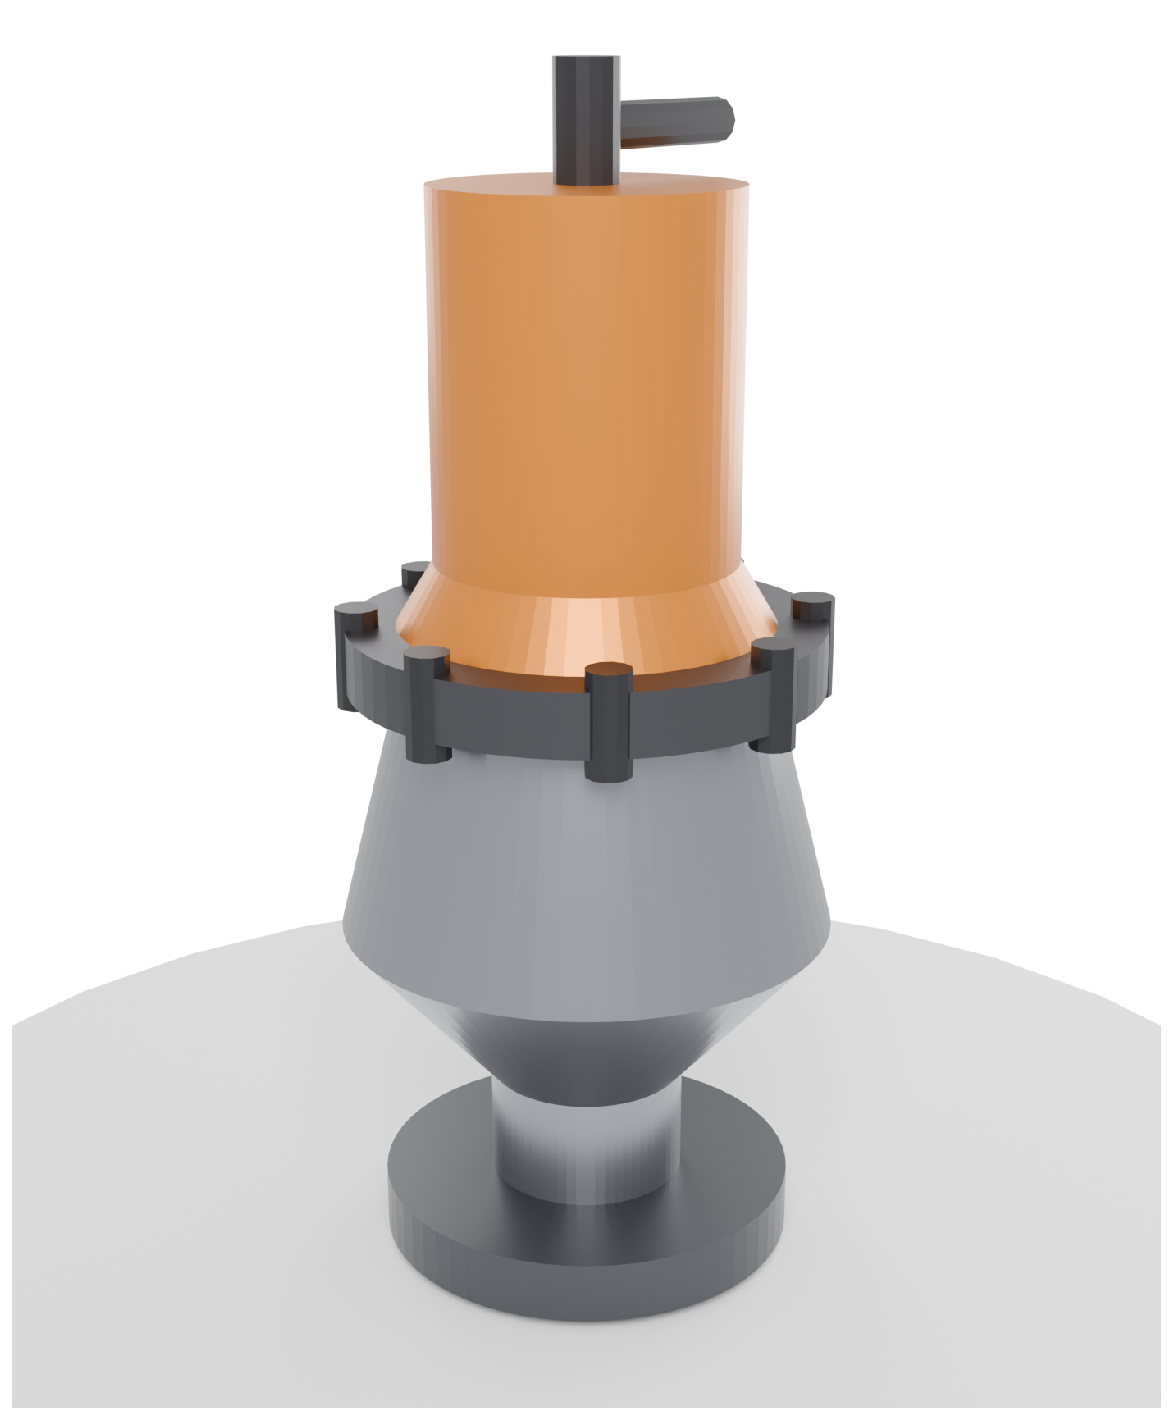
\includegraphics[width=0.40\textwidth]{figuras/fig_13_1_valvulas.pdf}
		\caption[Válvula de segurança industrial (PSV)]{Válvula de segurança (PSV) industrial, em perspectiva 3D — flange de entrada, corpo, flange do capuz, capuz da mola de ajuste e alavanca de teste manual. Esquema ilustrativo, não um desenho de projeto.}
		\label{fig:13-1}
	\end{figure}

	Quando a máquina passa para alívio, a válvula de \textit{blow-down} despressuriza o volume interno entre o elemento compressor e a válvula de retenção. Esse esvaziamento não é instantâneo: o ar escoa por um orifício de área fixa, e a pressão decai de forma aproximadamente exponencial a partir do valor de operação até a pressão de alívio residual, conforme a Equação~\eqref{eq:s13-5}. A constante de tempo $\tau_{bd}$ agrega a geometria do orifício de descarga e o volume a despressurizar — quanto maior o volume interno ou menor o orifício, mais lento o alívio:
	\begin{equation}\label{eq:s13-5}
 P(t) = P_{\text{alívio}} + (P_{\text{max}} - P_{\text{alívio}}) \cdotp e^{-t/\tau_{bd}}
\end{equation}
	O subscrito em $\tau_{bd}$ evita colisão com o torque $\tau$ dos capítulos de transmissão. Essa constante de tempo é diagnóstica por si só: um $\tau_{bd}$ que cresce ao longo dos meses indica orifício de \textit{blow-down} parcialmente obstruído, e a máquina passa a consumir potência comprimindo contra uma pressão interna que deveria já ter sido aliviada — perda energética que não aparece em nenhum indicador de regime permanente, apenas na transição.

	Para sistemas com inversor de frequência, a potência absorvida é descrita em função da frequência normalizada $\bar{f} = f/f_{\text{nom}}$ pela Equação~\eqref{eq:s13-6}:
	\begin{equation}\label{eq:s13-6}
 \dot{W}_{\text{vfd}} = \dot{W}_{\text{nominal}} \cdotp (a \cdotp \bar{f}^2 + b \cdotp \bar{f} + c)
\end{equation}
	Onde $a$, $b$ e $c$ são coeficientes ajustados aos dados da própria máquina. Cabe aqui uma advertência que é fonte recorrente de erro de modelagem: essa forma quadrática \textbf{não} é a lei de afinidade das turbomáquinas. Em um ventilador ou bomba centrífuga a potência varia com o cubo da rotação, e reduzir 20\% da velocidade economiza cerca de metade da energia. Um compressor de parafuso é uma máquina de deslocamento positivo: a vazão é proporcional à rotação e o trabalho específico de compressão praticamente não depende dela, de modo que a potência varia de forma \textbf{aproximadamente linear} com $\bar{f}$. O termo quadrático da Equação~\eqref{eq:s13-6} não representa a compressão em si — ele captura os desvios de segunda ordem: a variação de rendimento do motor e do inversor fora do ponto nominal, o aumento relativo das perdas por vazamento interno em baixa rotação (o tempo de contato por volta cresce, e a folga $\delta$ tem mais tempo para fugir ar) e as perdas mecânicas de atrito. Transportar a lei cúbica para este equipamento superestima grosseiramente a economia esperada de um VSD e leva a decisões de investimento erradas.

	\subsection{\textbf{Estratégias de Modulação em Comparação}}
	O título deste capítulo promete estratégias de modulação, e é aqui que elas se separam quantitativamente. A métrica correta para compará-las não é a potência absoluta, mas a \textbf{potência específica} — energia gasta por unidade de ar efetivamente entregue. Trata-se do mesmo $SPC$ definido como KPI global na Equação~\eqref{eq:s11-11}, aqui escrito como função da fração de carga para expor o que aquela forma agregada esconde. Sendo $x_c$ a fração da capacidade nominal realmente demandada pela planta ($x_c = \dot{V}_{\text{demanda}}/\dot{V}_{\text{nom}}$), a Equação~\eqref{eq:s13-7} define a potência específica e as duas leis de consumo que a alimentam:
	\begin{equation}\label{eq:s13-7}
	\text{SPC}(x_c) = \frac{\dot{W}(x_c)}{x_c \cdot \dot{V}_{\text{nom}}}, \qquad
	\begin{aligned}
	\dot{W}_{\text{c/a}}(x_c) &= \dot{W}_{\text{nom}} \left[ x_c + (1 - x_c) \, k_{ul} \right] \\
	\dot{W}_{\text{vsd}}(x_c) &\approx \dot{W}_{\text{nom}} \, \frac{x_c}{\eta_{vsd}(x_c)}
	\end{aligned}
	\end{equation}
	Onde $k_{ul} = \dot{W}_{\text{unload}}/\dot{W}_{\text{nom}}$ é a fração da potência nominal que a máquina continua consumindo em alívio, e $\eta_{vsd}(x_c)$ é o rendimento combinado de motor e inversor na carga parcial correspondente. Note que $k_{ul}$ não é um valor de tabela: ele é uma característica medida da máquina específica, e o Gêmeo Digital o extrai diretamente do histórico de operação, cruzando os períodos com $\delta = 0$ na Equação~\eqref{eq:s13-10} com a potência elétrica registrada no mesmo intervalo.

	A leitura da Equação~\eqref{eq:s13-7} explica por que a escolha de estratégia importa tanto. Na operação em carga/alívio, o numerador tem um piso — a máquina em alívio nunca consome zero — enquanto o denominador vai a zero com a demanda. A potência específica, portanto, \textbf{diverge} em baixa carga: uma planta operando cronicamente a 30\% da capacidade paga por cada metro cúbico um múltiplo do que pagaria em plena carga. Já na modulação por velocidade, numerador e denominador caem juntos, e a potência específica permanece aproximadamente plana até o limite inferior de rotação da máquina — abaixo do qual a lubrificação dos mancais e o resfriamento deixam de ser adequados, e a máquina precisa alternar para carga/alívio de qualquer forma. Esse limite inferior, e não a curva teórica, é o que define o ganho real do VSD em uma instalação concreta.

	\subsection{\textbf{Ciclagem, Banda Morta e Volume de Reservatório}}
	Uma máquina em carga/alívio não escolhe livremente sua frequência de ciclagem: ela é imposta pela demanda, pelo volume de rede disponível e pela banda morta de pressão configurada. Durante a carga, a rede pressuriza com a diferença entre o que o compressor entrega e o que a planta consome; durante o alívio, despressuriza apenas com o consumo. Aplicando a Equação~\eqref{eq:s13-4} a cada um dos dois trechos e somando as durações, obtém-se a frequência de ciclagem da Equação~\eqref{eq:s13-8}:
	\begin{equation}\label{eq:s13-8}
	f_{\text{ciclo}} = \frac{1}{t_{\text{carga}} + t_{\text{alívio}}} = \frac{R \cdot T \cdot \dot{m}_{\text{demanda}} \left( \dot{m}_{\text{comp}} - \dot{m}_{\text{demanda}} \right)}{V_{\text{net}} \cdot \Delta P_{db} \cdot \dot{m}_{\text{comp}}}
	\end{equation}
	Onde $\Delta P_{db}$ é a banda morta entre as pressões de corte e de religamento. A expressão tem um máximo em $\dot{m}_{\text{demanda}} = \dot{m}_{\text{comp}}/2$, isto é, a ciclagem é mais severa exatamente na demanda igual à metade da capacidade — não nos extremos, como a intuição sugeriria. Esse resultado é o que amarra este capítulo ao dimensionamento dos vasos pulmão: como $f_{\text{ciclo}}$ é inversamente proporcional a $V_{\text{net}}$ e a $\Delta P_{db}$, respeitar o número máximo de partidas por hora admitido pelo motor e pelo atuador da válvula é uma restrição que se satisfaz aumentando o volume de rede ou alargando a banda morta — e alargar a banda morta custa energia, pela sensibilidade que a subseção seguinte quantifica.

	\subsection{\textbf{Sensibilidade do Consumo ao \textit{Setpoint} de Pressão}}
	Toda decisão de controle que eleve a pressão de descarga — uma banda morta mais larga, uma margem de segurança adicional sobre a pressão mínima do processo — se paga em energia, e o Gêmeo Digital precisa quantificar esse custo antes de propor o ajuste. Partindo da potência de compressão politrópica, o consumo é proporcional a $\left(\Pi^{(n-1)/n} - 1\right)$, e a sensibilidade relativa da potência a uma variação relativa da razão de pressão é a elasticidade da Equação~\eqref{eq:s13-9}:
	\begin{equation}\label{eq:s13-9}
	E_{\Pi} = \frac{\partial \dot{W}/\dot{W}}{\partial \Pi/\Pi} = \frac{\dfrac{n-1}{n} \cdot \Pi^{(n-1)/n}}{\Pi^{(n-1)/n} - 1}
	\end{equation}
	O comportamento dessa elasticidade é o que torna a Equação~\eqref{eq:s13-9} útil na prática. Para uma razão de pressão global $\Pi = 8$ e índice politrópico $n = 1{,}35$, ela vale aproximadamente $0{,}62$: cada 1\% de aumento na pressão de descarga custa $0{,}62\%$ de potência adicional. Traduzido para a unidade com que o operador raciocina, elevar a descarga de $8$ para $9$ bar absolutos — um aumento de $12{,}5\%$ — custa cerca de $7\%$ a mais de energia, valor que se mantém entre $7{,}2\%$ e $7{,}6\%$ para $n$ entre $1{,}3$ e $1{,}4$, e que reproduz a regra prática de campo de ``aproximadamente 7\% por bar''. A diferença é que aqui ela não é uma regra decorada: é uma consequência calculável da termodinâmica do estágio, válida na faixa em que foi avaliada e recalculável pelo Gêmeo Digital para a condição real da máquina. Note ainda que $E_{\Pi}$ \textbf{cresce} conforme $\Pi$ diminui — em uma rede operando em pressão mais baixa, cada bar excedente pesa proporcionalmente mais, o que reforça a busca pelo \textit{setpoint} mínimo compatível com o processo.

	\subsection{\textbf{Matriz de Diagnóstico de Controle}}
	A Tabela~\ref{tab:13-1} cruza o comportamento da taxa de pressurização ($dP/dt$) com o consumo elétrico para localizar a origem de uma perda de eficiência pneumática — distinguindo vazamento interno, falha de válvula, filtro obstruído e vazamento externo à máquina.
	\begin{table}[H]
		\centering
		\resizebox{\textwidth}{!}{
			\begin{tabular}{l c c l}
				\toprule
				\textbf{Falha} & \textbf{Comportamento $dP/dt$} & \textbf{Consumo Elétrico} & \textbf{Diagnóstico Digital} \\ \midrule
				Vazamento \textit{Blow-off} & Baixo na Carga & $\uparrow$ SPC & \textbf{Perda de Eficiência Pneumática} \\
				Válvula Admissão Presa & Zero (não sobe) & $\downarrow$ (Vazio) & \textbf{Falha Mecânica no Atuador} \\
				Filtro Obstruído & Lento & $\downarrow$ Torque & \textbf{Manutenção Preventiva Filtro} \\
				Vazamento na Rede & Baixo (Carga/Alívio) & Constante & \textbf{Vazamento Externo à Máquina} \\ \bottomrule
			\end{tabular}
		}
		\caption[Matriz de diagnóstico do sistema de controle]{Matriz de diagnóstico do sistema de controle e válvulas de modulação.}
		\label{tab:13-1}
	\end{table}
	
	\subsection{\textbf{KPI Energético: Custo de Ciclo}}
	O custo operacional é integrado com base no estado binário da válvula de admissão $\delta$ (1 para Carga, 0 para Alívio), pela Equação~\eqref{eq:s13-10}:
	\begin{equation}\label{eq:s13-10}
 \boxed{C_{op} = \int_{t_1}^{t_2} (\dot{W}_{\text{load}} \cdotp \delta + \dot{W}_{\text{unload}} \cdotp (1 - \delta)) dt}
\end{equation}

	\vspace{1em}
	\hrule
	\vspace{1em}

	\textbf{Diretriz Técnica Final:} O custo de ciclo da Equação~\eqref{eq:s13-10} é a métrica que conecta a estratégia de modulação (carga/alívio) diretamente ao custo energético — qualquer ajuste de \textit{setpoint} de pressão proposto pelo Gêmeo Digital deve ser avaliado por seu impacto em $C_{op}$, não apenas pela estabilidade de pressão que produz. As três grandezas deste capítulo que tornam esse julgamento possível são a potência específica em carga parcial (Equação~\eqref{eq:s13-7}), a frequência de ciclagem imposta pelo par volume/banda morta (Equação~\eqref{eq:s13-8}) e a elasticidade do consumo à pressão de descarga (Equação~\eqref{eq:s13-9}) — e elas frequentemente puxam em direções opostas: alargar a banda morta protege o atuador da ciclagem excessiva, mas eleva a pressão média e o consumo. O papel do Gêmeo Digital não é otimizar uma delas isoladamente, e sim expor esse conflito quantificado ao MPC do Capítulo 24, que decide com todas as restrições à vista.

	\clearpage
	\section{Aftercooler, Filtragem Primária e Gestão de Condensado}
	
	Este capítulo detalha a modelagem do resfriamento posterior e da remoção de contaminantes líquidos. O Gêmeo Digital atua nesta etapa para garantir que o ar entregue à secadora PSA esteja dentro dos limites de temperatura e saturação, protegendo a integridade do material dessecante.
	
	\subsection{Termodinâmica do Aftercooler (Resfriador Posterior)}
	O aftercooler é o trocador de calor final do processo de geração. Sua função é reduzir a temperatura de descarga do estágio HP ($T_{d,hp}$) para níveis compatíveis com os elementos de filtragem e secagem. As duas grandezas que o descrevem — a efetividade e o coeficiente global de transferência — não são específicas deste equipamento: são as do método $\epsilon$--NTU e da definição de resistência térmica global, formulação-padrão de análise de trocadores de calor \cite[Cap.~11]{incropera}, aqui apenas particularizada para o par ar comprimido/água de resfriamento. A Figura~\ref{fig:14-1} mostra o aftercooler em perspectiva 3D, com um cabeçote aberto expondo o espelho tubular — é justamente essa superfície de tubos, multiplicada pelo número de unidades no feixe, que compõe a área $A$ da Equação~\eqref{eq:s14-2} adiante, e cuja obstrução progressiva (incrustação, depósito) é o que a monitoração de $U$ detecta.

	\begin{figure}[h!tbp]
		\centering
		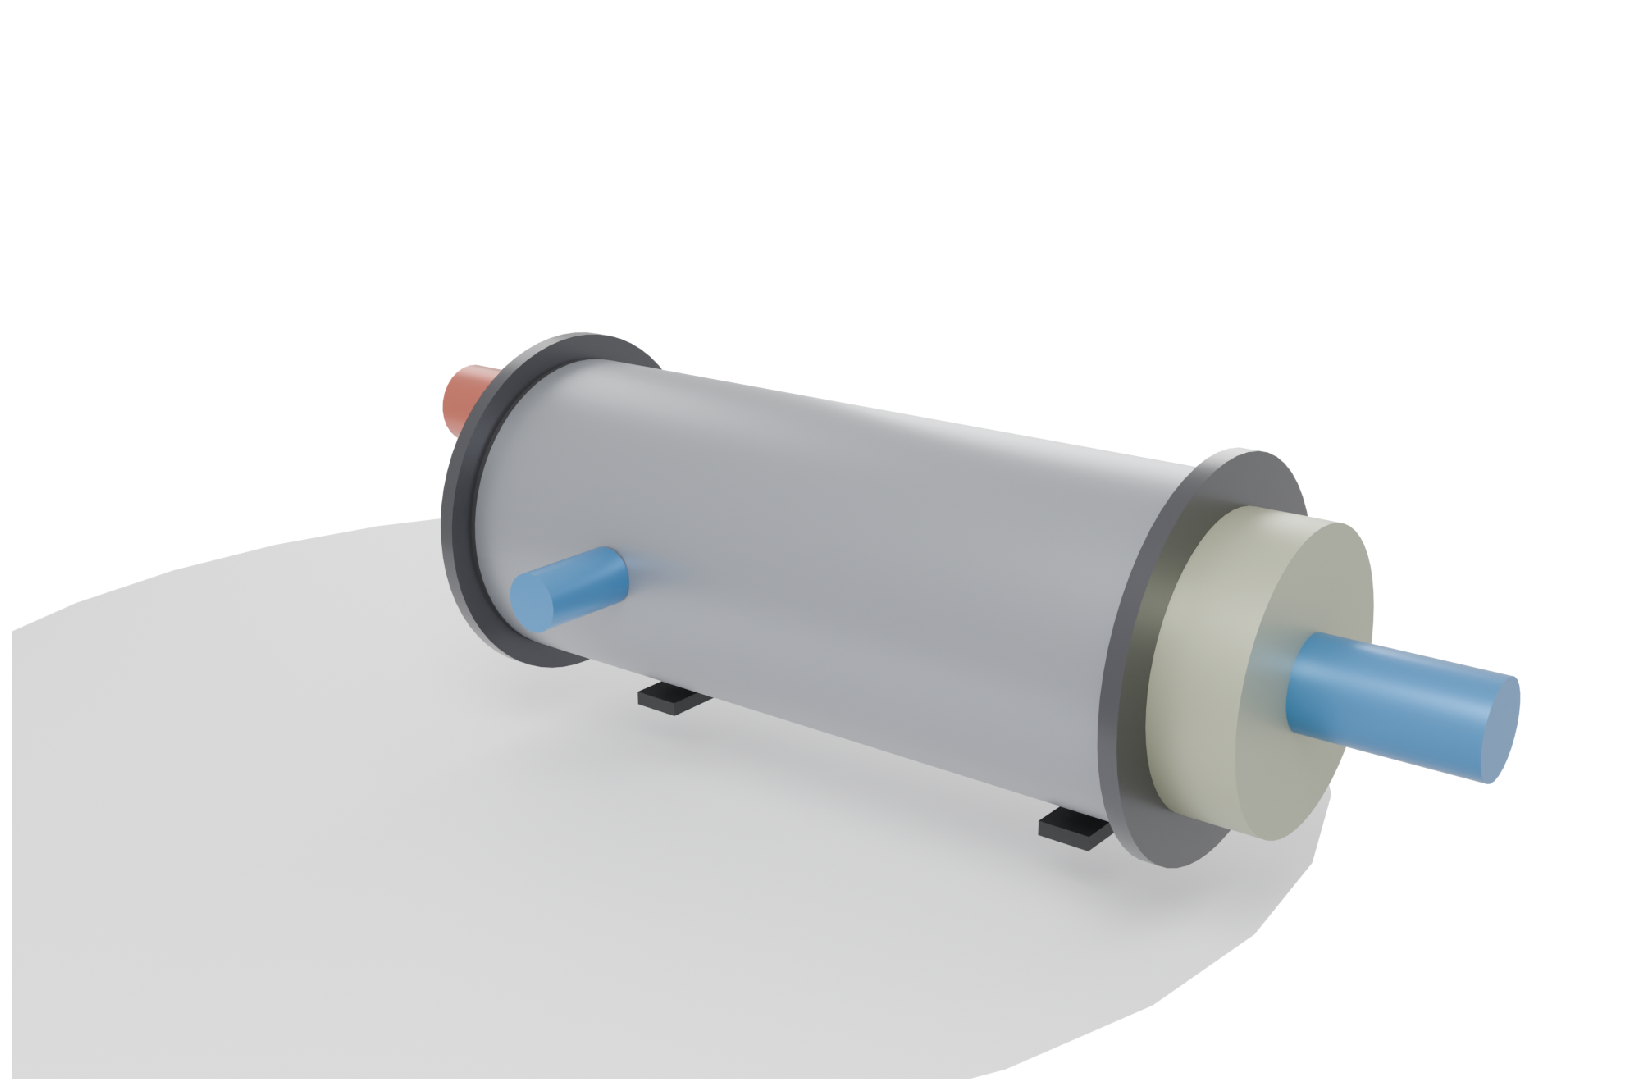
\includegraphics[width=0.75\textwidth]{figuras/fig_14_1_aftercooler.pdf}
		\caption[Trocador de calor casco-tubo, feixe de tubos exposto]{Aftercooler (trocador casco-tubo), em perspectiva 3D — cabeçote aberto expondo o espelho tubular, bocais de ar (quente/resfriado) e de água de resfriamento. Esquema ilustrativo, não um desenho de projeto.}
		\label{fig:14-1}
	\end{figure}

	\begin{itemize}
		\item \textbf{Efetividade Térmica ($\epsilon_{ac}$):} Mesma lógica de efetividade já usada no intercooler e no resfriador de óleo: a Equação~\eqref{eq:s14-1} compara a queda de temperatura real do ar ($T_{d,hp} - T_{ac,out}$) com a máxima queda teoricamente possível, limitada pela temperatura de entrada da água de resfriamento ($T_{d,hp} - T_{w,in}$):
		\begin{equation}\label{eq:s14-1}
 \epsilon_{ac} = \frac{T_{d,hp} - T_{ac,out}}{T_{d,hp} - T_{w,in}}
\end{equation}
		\item \textbf{Coeficiente Global de Transferência ($U$):} O modelo monitora a degradação por incrustação (\textit{fouling}), comum em ambientes offshore devido à salinidade, pela Equação~\eqref{eq:s14-2}:
		\begin{equation}\label{eq:s14-2}
 \dot{Q} = U \cdot A \cdot \Delta T_{LMTD} 
\end{equation}
		Onde $\Delta T_{LMTD}$ é a diferença de temperatura média logarítmica. Um desvio negativo persistente em $U$ sinaliza a necessidade de manutenção preditiva no trocador \cite{mobley}.
	\end{itemize}
	
	\subsection{Modelagem da Condensação e Separação de Umidade}
	A redução da temperatura sob alta pressão provoca a transição de fase do vapor d'água para o estado líquido. A Figura~\ref{fig:14-2} esquematiza o separador ciclônico logo a seguir descrito: o ar úmido entra tangencialmente, o corpo cônico acelera o escoamento em espiral e a força centrífuga lança as gotículas mais densas contra a parede, de onde escorrem para o dreno na base, enquanto o ar já separado sai pelo tubo central (\textit{vortex finder}) no topo — é exatamente essa velocidade tangencial excessiva, mencionada no item seguinte, que compromete essa separação e causa o arraste.

	\begin{figure}[h!tbp]
		\centering
		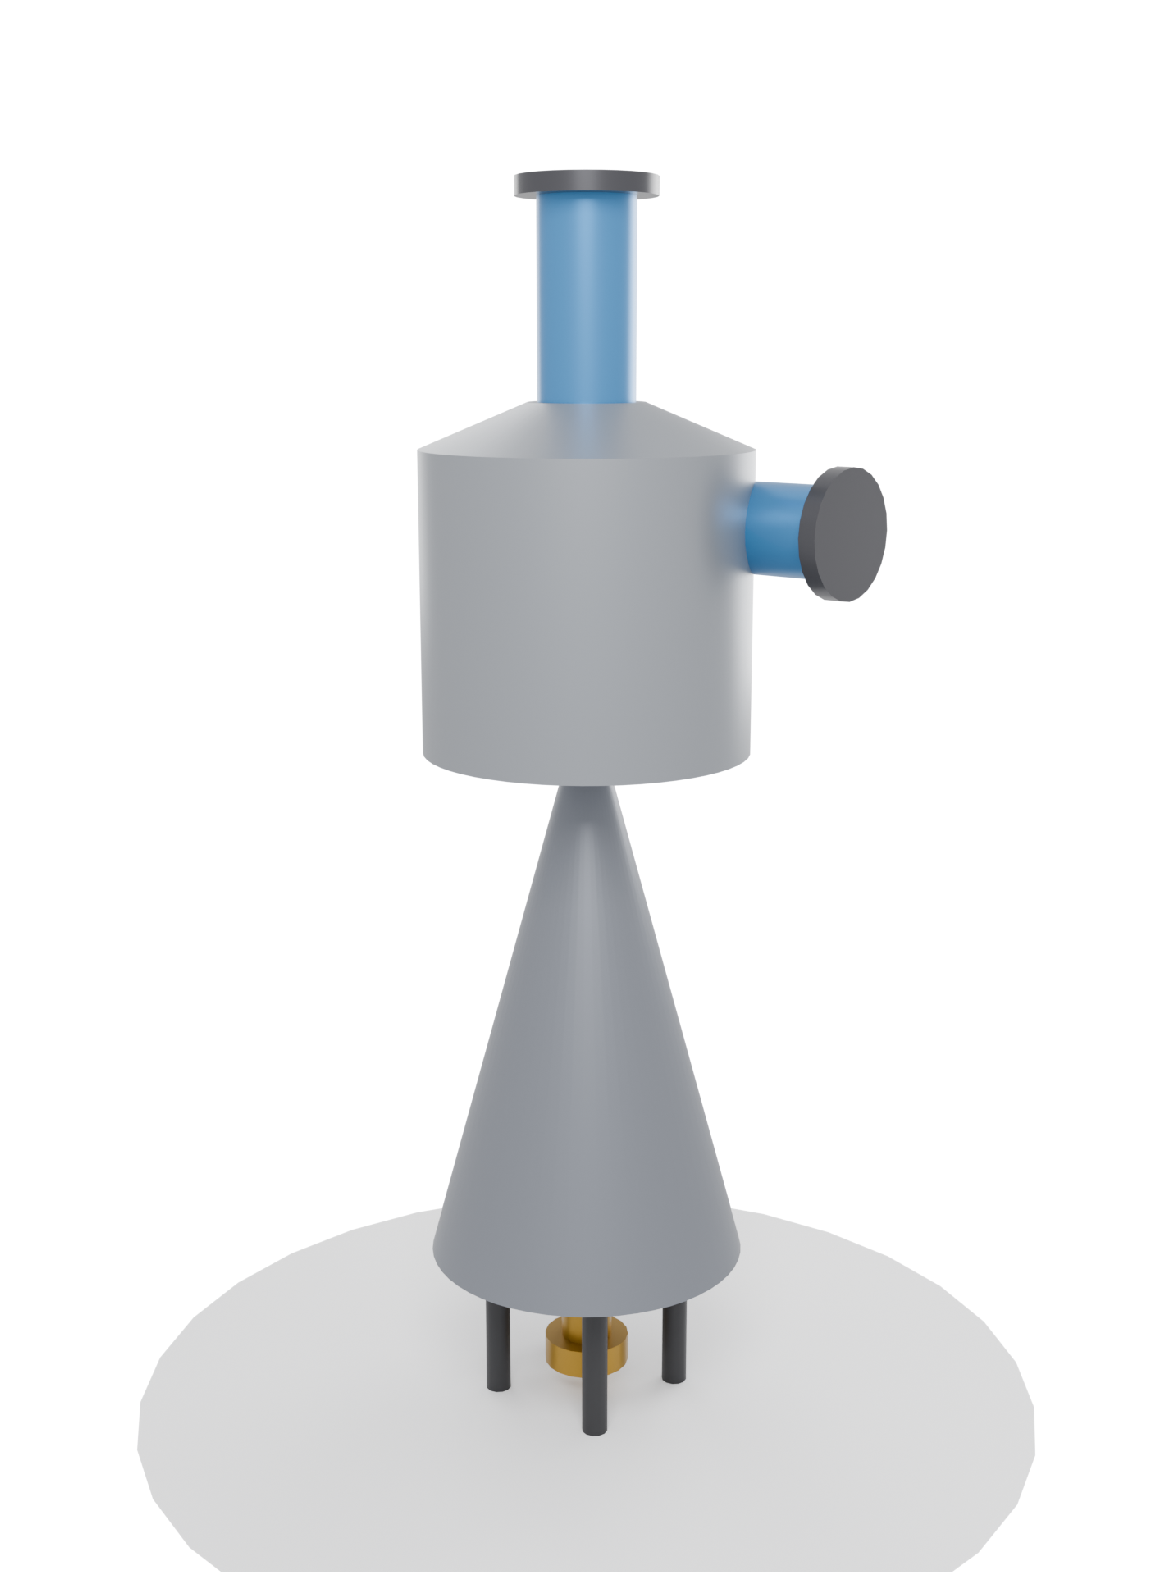
\includegraphics[width=0.42\textwidth]{figuras/fig_14_2_separador.pdf}
		\caption[Separador ciclônico de condensado]{Separador ciclônico de condensado, em perspectiva 3D — entrada tangencial, corpo cônico, saída de ar central e dreno de condensado na base. Esquema ilustrativo, não um desenho de projeto.}
		\label{fig:14-2}
	\end{figure}

	\begin{itemize}
		\item \textbf{Taxa de Condensação Mássica ($\dot{m}_{cond}$):} Toda a água que o ar carregava na entrada, acima do que ele ainda consegue reter na saturação à temperatura de saída, precipita como líquido — a Equação~\eqref{eq:s14-3} calcula essa massa de condensado como a vazão de ar seco vezes a queda na razão de umidade:
		\begin{equation}\label{eq:s14-3}
 \dot{m}_{cond} = \dot{m}_a \cdot (W_{in} - W_{sat,out})
\end{equation}
		Onde $W$ é a razão de umidade (kg de água por kg de ar seco). O Gêmeo Digital calcula $W_{sat,out}$ utilizando a pressão de saturação do vapor na temperatura de saída $T_{ac,out}$. A mesma ressalva do intercooler (Equação~\eqref{eq:s10-9}) se aplica aqui: a Equação~\eqref{eq:s14-2} soma apenas a parcela sensível de $\dot{Q}$, e a forma completa deve incluir o calor latente liberado por $\dot{m}_{cond}$ — $\dot{Q}_{\text{total}} = \dot{m}_a \cdot c_{p,\text{úmido}} \cdot (T_{d,hp} - T_{ac,out}) + \dot{m}_{cond} \cdot h_{fg}(T_{ac,out})$, mesma $h_{fg}(T)$ em $\text{J}\,\text{kg}^{-1}$ da Equação~\eqref{eq:s10-9} (unidades SI compatíveis com $c_{p,\text{úmido}}$, sem fator de conversão implícito).
		\item \textbf{Eficiência de Separação ($\eta_{sep}$):} O separador mecânico (ciclone) deve remover a fase líquida. O arraste de gotículas (\textit{carry-over}) é modelado como uma falha de separação por excesso de velocidade, pela Equação~\eqref{eq:s14-4}:
		\begin{equation}\label{eq:s14-4}
 \dot{m}_{arraste} = \dot{m}_{cond} \cdot (1 - \eta_{sep}) 
\end{equation}
	\end{itemize}
	
	\subsection{Dinâmica de Filtragem Coalescente}
	Os pré-filtros removem aerossóis de óleo e particulados. A perda de carga ($\Delta P$) é monitorada e normalizada pela densidade e vazão.
	\begin{itemize}
		\item \textbf{Equação de Perda de Carga:} Mesma forma de perda de carga localizada já usada para o filtro de admissão (Equação~\eqref{eq:s5-4}), agora aplicada ao filtro coalescente \cite{atlascopco}: proporcional ao coeficiente do elemento filtrante $\zeta_{\text{coal}}$ (mesma grandeza física de $\zeta$ na Equação~\eqref{eq:s5-4}, subscrito por ser um valor de projeto próprio do elemento coalescente) e à pressão dinâmica do escoamento, pela Equação~\eqref{eq:s14-5}:
		\begin{equation}\label{eq:s14-5}
 \Delta P_{filt} = \zeta_{\text{coal}} \cdot \frac{\rho \cdot v^2}{2}
\end{equation}
		\item \textbf{Diagnóstico de Saturação:} O modelo diferencia a perda de carga nominal da saturação por óleo ou água. Se $\Delta P_{filt} > \Delta P_{limit}$, o Gêmeo Digital emite um alerta de substituição para evitar o colapso do meio filtrante e a contaminação da secadora.
	\end{itemize}
	
	\subsection{Gestão de Drenos Automáticos e Purga}
	Os drenos são componentes críticos com alta taxa de falha mecânica em plataformas.
	\begin{itemize}
		\item \textbf{Falha Travado Aberto (\textit{Stuck Open}):} Causa perda de ar comprimido, elevando o consumo específico ($SPC$). Como a razão entre a pressão atmosférica (jusante) e a pressão de rede (montante) fica abaixo da razão crítica $r_{cr}$ — mesma convenção $r=P_{\text{jusante}}/P_{\text{montante}}$ da Equação~\eqref{eq:s13-2} —, o escoamento pelo orifício do dreno satura em regime sônico (\textit{choked flow}): a vazão mássica deixa de depender da pressão a jusante e passa a ser função apenas das condições a montante, seguindo a forma clássica de escoamento compressível em bocais convergentes \cite{white}, pela Equação~\eqref{eq:s14-6}:
		\begin{equation}\label{eq:s14-6}
 \dot{m}_{perda} = C_d \cdot A_{dreno} \cdot \sqrt{\gamma \rho P \left( \frac{2}{\gamma+1} \right)^{\frac{\gamma+1}{\gamma-1}}}
\end{equation}
		Onde $C_d$ é o coeficiente de descarga do orifício, $A_{dreno}$ sua área efetiva, e $\rho$, $P$ e $\gamma$ a densidade, pressão absoluta e razão de calores específicos do ar na rede a montante do dreno. A Equação~\eqref{eq:s14-6} é o ramo bloqueado da função de escoamento $\Phi(r)$ da Equação~\eqref{eq:s13-2}, particularizado para o caso do dreno, em que a razão de pressões está sempre muito abaixo da crítica ($r_{cr} \approx 0{,}528$ para o ar) porque a descarga se dá diretamente na atmosfera.
		\item \textbf{Falha Travado Fechado (\textit{Stuck Closed}):} Causa o alagamento do separador e arraste de água líquida para a secadora PSA, degradando o dessecante instantaneamente.
	\end{itemize}
	
	\subsection{Matriz de Diagnóstico de Tratamento Primário}
	A Tabela~\ref{tab:14-1} cruza os sintomas de temperatura, perda de carga nos filtros e umidade de saída para diferenciar incrustação do aftercooler, saturação de filtro e falha de dreno (aberto ou fechado).

	\begin{table}[h!tbp]
		\centering
		\resizebox{\textwidth}{!}{
		\begin{tabular}{l l l l l}
			\toprule
			\textbf{Evento} & \textbf{Temperatura Saída} & \textbf{$\Delta P$ Filtros} & \textbf{Umidade Saída} & \textbf{Diagnóstico Digital} \\
			\midrule
			Incrustação AC & $\uparrow$ (Elevada) & Nominal & $\uparrow$ (Vapor) & \textbf{Baixa Troca Térmica} \\
			Filtro Saturado & Nominal & $\uparrow \uparrow$ & Nominal & \textbf{Troca de Elemento} \\
			Dreno Aberto & Nominal & $\downarrow$ & Nominal & \textbf{Vazamento de Ar} \\
			Dreno Fechado & Nominal & $\uparrow$ (Oscilante) & $\uparrow \uparrow$ (Líquida) & \textbf{Risco de Alagamento} \\
			\bottomrule
		\end{tabular}
		}
		\caption[Matriz de diagnóstico de tratamento primário]{Matriz de diagnóstico de tratamento primário.}
		\label{tab:14-1}
	\end{table}

	\subsection{KPI de Performance de Tratamento (\texorpdfstring{$KPI_{treat}$}{KPI treat})}
	O indicador de saúde deste estágio, na Equação~\eqref{eq:s14-7}, valida se o ar está sendo resfriado o suficiente para maximizar a remoção de água antes da secagem química — mesma lógica de efetividade da Equação~\eqref{eq:s14-1} ($\epsilon_{ac}$), mas comparando o ponto de orvalho realmente alcançado, não a temperatura do ar:
	\begin{equation}\label{eq:s14-7}
 \boxed{KPI_{treat} = \frac{T_{d,hp} - T_{dew,actual}}{T_{d,hp} - T_{w,in}}}
\end{equation}

	\vspace{1em}
	\hrule
	\vspace{1em}

	\textbf{Diretriz Técnica Final:} Um $KPI_{treat}$ próximo de 1 na Equação~\eqref{eq:s14-7} indica que o ponto de orvalho efetivamente alcançado ($T_{dew,actual}$) está próximo da temperatura da água de resfriamento — condição necessária para proteger o leito dessecante do secador PSA a jusante; valores decrescentes aqui devem disparar investigação \textbf{antes} que o ponto de orvalho no secador seja afetado, não depois. O denominador usa $T_{d,hp}$ (descarga do estágio HP, mesma referência fixa da Equação~\eqref{eq:s14-1}), não $T_{ac,out}$: com $T_{ac,out}$ no denominador, o próprio ato de o aftercooler funcionar bem ($T_{ac,out} \to T_{w,in}$) zeraria o denominador e faria o índice divergir, em vez de convergir para 1 — o oposto do pretendido.

		\clearpage
		\section{\textbf{Sistema de Secagem por Adsorção (PSA e Tambor Rotativo)}}
		
		O sistema de secagem representa o estágio final de tratamento no Gêmeo Digital, monitorando a remoção de vapor de água para atingir o Ponto de Orvalho sob Pressão ($PDP$). O sistema integra torres de adsorção oscilante (\textbf{PSA}) e secadores de \textbf{tambor rotativo} por calor de compressão (HOC). A Figura~\ref{fig:15-1} ilustra o princípio de operação alternada das duas torres: enquanto uma adsorve umidade do ar de processo (A), a outra é regenerada (D) pela expansão de parte do ar já seco, e os papéis se invertem ciclicamente — o ar úmido entra (I), o ar seco sai (O) e a purga de regeneração é exaurida (E).

		\begin{figure}[h!tbp]
			\centering
			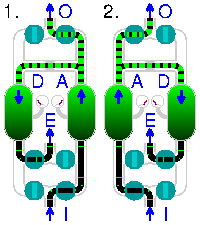
\includegraphics[width=0.75\textwidth]{figuras/fig_15_1_psa.pdf}
			\caption[Princípio de operação das torres PSA]{Princípio de operação das torres PSA em ciclos alternados de adsorção (A) e regeneração/dessorção (D). I = entrada de ar úmido, O = saída de ar seco, E = exaustão da purga. Fonte: \textit{Pressure swing adsorption principle}, Cmglee, Wikimedia Commons, licença CC BY-SA 4.0.}
			\label{fig:15-1}
		\end{figure}

		\subsection{\textbf{Cinética de Adsorção e Balanço de Massa}}
		
		O Gêmeo Digital modela a Zona de Transferência de Massa (MTZ) para prever a saturação do leito dessecante.
		
		\begin{itemize}
			\item \textbf{Capacidade de Adsorção Dinâmica ($q_d$):} A Equação~\eqref{eq:s15-1} descreve como a capacidade do leito dessecante de reter umidade decai exponencialmente ao longo do ciclo de adsorção, partindo da capacidade de equilíbrio e caindo à medida que a razão entre o tempo já decorrido e o tempo de residência do ar no leito aumenta:
			\begin{equation}\label{eq:s15-1}
q_d = q_{eq} \cdot \exp \left( -k_{ads} \cdot \frac{t_{ads}}{t_{res}} \right)
\end{equation}
			Onde $q_{eq}$ é a capacidade de adsorção em equilíbrio (isoterma do dessecante), $t_{ads}$ o tempo decorrido de adsorção, $t_{res}$ o tempo de residência do ar no leito, e $k_{ads}$ é a constante de taxa de adsorção do material dessecante (obtida experimentalmente, específica da alumina ativada ou peneira molecular empregada; subscrito para não colidir com $k$ do relé IEC 60255 ou o índice de tempo discreto usado nos capítulos de EKF/MPC/PSO). A Figura~\ref{fig:15-2} mostra como um $k_{ads}$ maior — leito mais fino, mais contaminado ou material dessecante degradado — acelera drasticamente a saturação, esgotando a capacidade útil do leito muito antes do fim do ciclo programado.

			\begin{figure}[h!tbp]
				\centering
				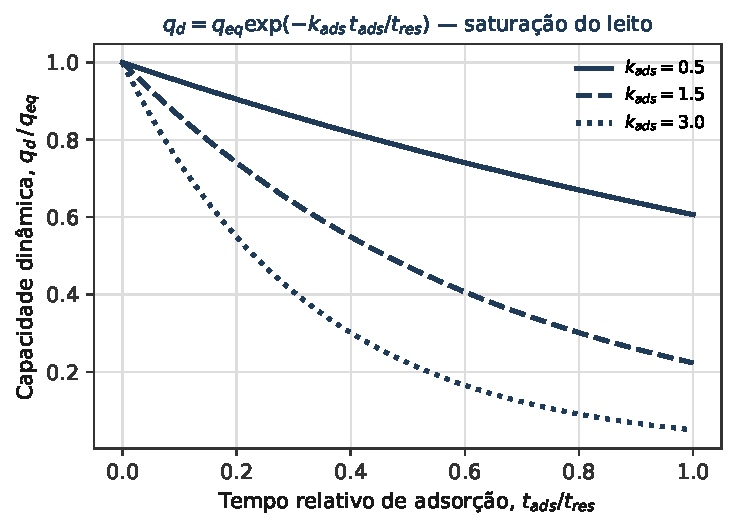
\includegraphics[width=0.60\textwidth]{figuras/fig_15_2_adsorcao.pdf}
				\caption[Capacidade de adsorção dinâmica normalizada]{Capacidade de adsorção dinâmica normalizada em função do tempo relativo de adsorção, para diferentes constantes de taxa $k_{ads}$.}
				\label{fig:15-2}
			\end{figure}

			\item \textbf{Vazão de Purga de Regeneração ($\dot{m}_{purge}$):}
			Calculada pela Equação~\eqref{eq:s15-2} para compensar a histerese de adsorção com o fator $\phi$:
			\begin{equation}\label{eq:s15-2}
\dot{m}_{purge} = \dot{m}_{in} \cdot \left( \frac{P_{low}}{P_{high}} \right) \cdot \phi
\end{equation}
			
			\item \textbf{Balanço de Umidade Acumulada:} A Equação~\eqref{eq:s15-3} encadeia três grandezas: primeiro a queda na razão de umidade entre entrada e saída do leito ($\Delta W$), depois a vazão mássica de água efetivamente retida ($\dot{m}_{water}$, obtida multiplicando $\Delta W$ pela vazão de ar seco), e por fim a massa total de água acumulada no leito ($M_{ads}$) integrando essa vazão ao longo de todo o ciclo de adsorção — usada para prever quando o leito se aproxima da saturação:
			\begin{equation}\label{eq:s15-3}
			\begin{aligned}
				\Delta W &= W_{in} - W_{out} \\[4pt]
				\dot{m}_{water} &= \dot{m}_a \cdot (W_{in} - W_{out}) \\[4pt]
				M_{ads}(t) &= \int_0^{t_{cycle}} \dot{m}_{water} \, dt
			\end{aligned}
\end{equation}
		\end{itemize}

		\subsection{\textbf{Cinética de Regeneração e Propriedades do Material Dessecante}}

		A Equação~\eqref{eq:s15-1} descreve como a capacidade do leito decai durante a adsorção, mas o processo inverso — a regeneração térmica que devolve essa capacidade — permanecia, até esta revisão, descrito apenas qualitativamente neste documento. A mesma forma exponencial de 1ª ordem que governa a adsorção descreve, por simetria física, a recuperação de capacidade durante a regeneração: um processo de transporte de massa/calor limitado por uma força motriz que diminui à medida que o leito se aproxima do equilíbrio — não uma reta com uma quina abrupta no fim da fase, fisicamente implausível para um leito real. A Equação~\eqref{eq:s15-12} formaliza essa recuperação:

		\begin{equation}\label{eq:s15-12}
		q_d(t_{regen}) = q_{eq} - \left(q_{eq} - q_{d,0}\right) \cdot \exp\left(-\kappa_{regen} \cdot \frac{t_{regen}}{t_{regen,ciclo}}\right)
		\end{equation}

		Onde $q_{d,0}$ é a capacidade remanescente ao final da fase de adsorção (o valor de $q_d$ da Equação~\eqref{eq:s15-1} no instante da troca), $t_{regen}$ o tempo decorrido de regeneração, $t_{regen,ciclo}$ a duração total programada da fase, e $\kappa_{regen}$ a constante de taxa da recuperação — análoga a $k_{ads}$, mas para o processo reverso, tipicamente maior (dessorção forçada por um aquecedor de regeneração costuma ser mais rápida que a adsorção passiva à temperatura ambiente). O mesmo perfil exponencial descreve a temperatura do leito durante a regeneração e o resfriamento subsequente — a resposta térmica de uma massa aquecida ou resfriada por convecção é, por construção, de 1ª ordem, nunca uma rampa linear.

		A constante $\kappa_{regen}$, como $k_{ads}$, depende do material dessecante empregado — e o próprio $q_{eq}$ da Equação~\eqref{eq:s15-1} nunca foi, até aqui, associado a um valor numérico concreto neste documento, apenas descrito como ``a isoterma do dessecante''. A Tabela~\ref{tab:15-2} fecha essa lacuna para os três materiais mais comuns em secadores PSA de ar comprimido offshore, com densidade aparente e capacidade de \textbf{trabalho} — a fração mássica de água retida em \textbf{baixa} umidade relativa, o regime real de um secador a jusante de aftercooler e separador (Capítulo 14), sempre menor que a capacidade estática máxima de folha de dados de fabricante (medida em alta UR, condição que o leito nunca alcança em serviço PSA):

		\begin{table}[h!tbp]
			\centering
			\resizebox{\textwidth}{!}{
			\begin{tabular}{l c c c c c}
				\toprule
				\textbf{Material} & \textbf{Densidade [kg/m³]} & \textbf{Capacidade $q_{eq}$} & \textbf{$k_{ads}$ Ref.} & \textbf{$t_{regen}$ Ref. [min]} & \textbf{$t_{resfriamento}$ Ref. [min]} \\ \midrule
				Alumina Ativada & 750 & 10\% & 1,5 & 45 & 10 \\
				Sílica Gel & 700 & 8\% & 1,2 & 45 & 10 \\
				Peneira Molecular 13X & 720 & 18\% & 1,8 & 45 & 10 \\ \bottomrule
			\end{tabular}
			}
			\caption[Propriedades de referência dos materiais dessecantes]{Propriedades de referência dos materiais dessecantes mais comuns em secadores PSA de ar comprimido — densidade aparente e capacidade de trabalho em baixa UR (ASSUMIDO, faixas típicas de literatura/fabricante), constante de taxa de adsorção e tempos de regeneração/resfriamento de referência.}
			\label{tab:15-2}
		\end{table}

		É a peneira molecular, não a alumina ativada (o material mais citado como padrão de mercado para ar comprimido), que oferece a maior capacidade de trabalho em baixa UR e o menor ponto de orvalho alcançável — o que a torna preferível quando a especificação normativa exige a Classe 2 da ISO 8573-1 (PDP alvo de $-40\,^{\circ}\text{C}$, já adotada neste documento no Capítulo 18) com folga de projeto. A sílica gel, por desempenho fraco em baixa UR, raramente é usada isoladamente para esse alvo — sua aplicação típica é em umidade relativa mais alta, fora do regime de um secador de ar comprimido já pré-secado.

		Vale uma ressalva de proveniência, na mesma linha da distinção já feita neste documento entre parâmetro medido, inferível, calibrável e desconhecido (Tabela~\ref{tab:28-1}): só os tempos de regeneração e resfriamento da \textbf{Alumina Ativada} na Tabela~\ref{tab:15-2} vêm de experiência de campo relatada pelo autor (16/08/2026) — os mesmos valores foram reaproveitados por analogia para os outros dois materiais, sem fonte própria verificada. Os valores de $k_{ads}$ de referência, para os três materiais, \textbf{não} foram verificados contra literatura nem ensaio — representam apenas uma ordenação relativa plausível (peneira molecular mais rápida, sílica mais lenta), não uma medição. As duas lacunas ficam registradas aqui deliberadamente, pela mesma disciplina de transparência já adotada para outros parâmetros ASSUMIDOS deste documento, em vez de apresentar precisão que os dados não sustentam.

		Com a capacidade de trabalho da Tabela~\ref{tab:15-2} e a massa real do leito por torre ($M_{leito}$, um dado de projeto), a Equação~\eqref{eq:s15-13} converte a capacidade normalizada da Equação~\eqref{eq:s15-1} em massa física de água retida — uma alternativa prática ao balanço rigoroso da Equação~\eqref{eq:s15-3}, útil quando não há um sensor contínuo de $W_{out}$ na saída do leito, apenas o modelo cinético da Eq. 15.1 e a especificação do material:

		\begin{equation}\label{eq:s15-13}
		M_{ads,cap}(t) = \left[q_{eq} - q_d(t)\right] \cdot M_{leito}
		\end{equation}

		As duas estimativas de massa de água — o balanço mássico direto (Equação~\eqref{eq:s15-3}, exige $W_{out}$ medido) e a baseada em capacidade (Equação~\eqref{eq:s15-13}, exige só a cinética e a especificação do material) — deveriam concordar num leito saudável; uma divergência persistente entre elas é, por si só, um sintoma diagnóstico: indica que a capacidade real do material já não corresponde ao valor de catálogo da Tabela~\ref{tab:15-2}, tipicamente por contaminação (óleo carreado por falha do separador, Capítulo 14) ou envelhecimento do próprio dessecante.

		O próprio $t_{res}$ da Equação~\eqref{eq:s15-1} — descrito ali como ``tempo de residência do ar no leito'', mas nunca antes desta revisão calculado a partir de nenhum dado de projeto — se fecha pela mesma via de balanço de massa de água da Equação~\eqref{eq:s15-13}: o tempo que o leito, na capacidade de trabalho do material selecionado e na carga de umidade do ar de entrada, levaria para saturar totalmente à vazão de projeto. A Equação~\eqref{eq:s15-14} formaliza esse fechamento:

		\begin{equation}\label{eq:s15-14}
		t_{res} = \frac{M_{leito} \cdot q_{eq}}{60 \cdot \dot{m}_{ar} \cdot W_{in}}
		\end{equation}

		Onde $\dot{m}_{ar}$ é a vazão mássica de ar a secar [kg/s] (mesma variável da Equação~\eqref{eq:s15-2}) e $W_{in}$ a razão de umidade do ar que chega ao secador (Equação~\eqref{eq:s10-6}), calculada a partir do ponto de orvalho de entrada; o fator 60 converte de segundos para minutos, a mesma unidade de $t_{ads}$ na Equação~\eqref{eq:s15-1}. A consequência prática fecha exatamente a lacuna que motivou esta equação: mais massa de dessecante, à mesma vazão e umidade, aumenta $t_{res}$ proporcionalmente — e, pela própria Equação~\eqref{eq:s15-1}, esgota o leito mais devagar e sustenta o ponto de orvalho de saída mais perto do alvo por mais tempo. Sem essa relação, a massa do leito seria um parâmetro de projeto sem nenhum efeito sobre o desempenho do secador no modelo — uma inconsistência física real, identificada ao testar uma versão anterior desta seção que ainda tratava $t_{res}$ como parâmetro independente da massa do leito.

		\subsection{\textbf{Termodinâmica do Secador de Tambor Rotativo (HOC)}}
		
		Este subsistema utiliza o calor residual do estágio de alta pressão ($HP$) para regenerar a matriz dessecante.
		
		\begin{itemize}
			\item \textbf{Efetividade de Regeneração Térmica ($\eta_{reg}$):} Mesmo princípio de efetividade usado nos trocadores de calor do documento: a Equação~\eqref{eq:s15-4} compara a queda real de temperatura do ar de regeneração com a máxima queda possível, limitada pela temperatura ambiente:
			\begin{equation}\label{eq:s15-4}
\eta_{reg} = \frac{T_{reg,in} - T_{reg,out}}{T_{reg,in} - T_{amb}}
\end{equation}
			
			\item \textbf{Velocidade de Rotação Crítica ($\omega_{drum}$):}
			Ajustada dinamicamente pela Equação~\eqref{eq:s15-5} para evitar o \textit{carry-over} de umidade:
			\begin{equation}\label{eq:s15-5}
\omega_{drum} \propto \frac{\dot{m}_a}{\rho_a \cdot C_p \cdot \Delta T_{ads}}
\end{equation}
		\end{itemize}

		\subsection{\textbf{Aproveitamento de Calor Rejeitado na Regeneração}}
		O ciclo HOC já aproveita o calor residual do próprio ar de descarga do estágio HP para aquecer o dessecante, mas esse não é o único calor rejeitado disponível na planta: o aftercooler (Equação~\eqref{eq:s14-2}), o resfriador de óleo (Capítulo de Sistema de Lubrificação e Gestão Térmica) e agora a exaustão forçada do invólucro do pacote (Equação~\eqref{eq:s2-2}) rejeitam calor de baixa/média qualidade que hoje é simplesmente descartado para o ambiente ou para a água de resfriamento. Recuperar parte desse calor para pré-aquecer o ar de regeneração reduz diretamente a potência elétrica que o aquecedor resistivo precisa fornecer.
		\begin{itemize}
			\item \textbf{Calor Residual Disponível para Recuperação ($\dot{Q}_{\text{disp}}$):} A soma das rejeições térmicas das correntes candidatas a um trocador de recuperação de calor, pela Equação~\eqref{eq:s15-10}:
			\begin{equation}\label{eq:s15-10}
\dot{Q}_{\text{disp}} = \dot{Q}_{\text{aftercooler}} + \dot{Q}_{\text{óleo}} + \dot{Q}_{\text{hood}}
\end{equation}
			\item \textbf{Potência do Aquecedor com Recuperação:} A Equação~\eqref{eq:s15-11} reduz a demanda do aquecedor elétrico de regeneração na proporção do calor efetivamente recuperado, limitada pela efetividade do trocador de recuperação ($\epsilon_{\text{recup}}$, mesma definição de efetividade da Equação~\eqref{eq:s15-4}) e nunca abaixo de zero:
			\begin{equation}\label{eq:s15-11}
\dot{W}_{\text{heater,real}} = \max\left(0,\; \dot{W}_{\text{heater,nom}} - \epsilon_{\text{recup}} \cdot \dot{Q}_{\text{disp}}\right)
\end{equation}
			Substituindo $\dot{W}_{\text{heater}}$ por $\dot{W}_{\text{heater,real}}$ na Equação~\eqref{eq:s15-6}, o Gêmeo Digital quantifica em tempo real quanto a recuperação de calor está reduzindo o $SEC_{dry}$ — e pode sinalizar quando o trocador de recuperação está subdimensionado ou incrustado, caso $\epsilon_{\text{recup}}$ medido caia abaixo do valor de projeto sem justificativa de carga térmica.
		\end{itemize}

		\subsection{\textbf{Soprador Booster e Fechamento Convectivo do Aquecedor}}
		Até este ponto, a temperatura do ar que entra no leito durante a regeneração ($T_{reg,in}$, usada na Equação~\eqref{eq:s15-4}) é tratada como um patamar dado — o quanto o aquecedor resistivo eleva a temperatura do ar acima da entrada não é derivado de nenhuma física de troca térmica. Essa lacuna importa na prática: o elemento resistivo só aquece o ar que efetivamente escoa em contato com ele, e esse contato é convectivo — sem um \textbf{soprador booster} forçando vazão suficiente através do aquecedor, o coeficiente de convecção $h$ despenca para a faixa de convecção natural, e o mesmo aquecedor de potência nominal fixa entrega um $\Delta T$ real muito menor do que o projeto pressupõe (o excesso de potência simplesmente eleva a temperatura do próprio elemento resistivo, não a do ar, até o limite de segurança do elemento). O soprador booster existe justamente para evitar esse regime: ele impõe a vazão de ar de regeneração ($\dot{m}_{reg}$, tipicamente distinta e menor que a vazão principal de processo) que mantém o escoamento em regime turbulento forçado sobre o elemento aquecedor.

		A vazão imposta pelo booster fixa o número de Reynolds do escoamento através do duto/banco de aquecedores, e a correlação clássica de Dittus-Boelter para convecção forçada turbulenta em duto \cite[Cap.~8]{incropera} fecha o coeficiente de convecção resultante, pela Equação~\eqref{eq:s15-15}:
		\begin{equation}\label{eq:s15-15}
		\begin{aligned}
			Re_{reg} &= \frac{4 \, \dot{m}_{reg}}{\pi \, D_h \, \mu_{ar}} \\[4pt]
			Nu &= 0{,}023 \, Re_{reg}^{0{,}8} \, Pr^{0{,}4} \\[4pt]
			h &= \frac{Nu \cdot k_{ar}}{D_h}
		\end{aligned}
	\end{equation}
		Onde $D_h$ é o diâmetro hidráulico do duto/banco de resistências, $\mu_{ar}$ e $k_{ar}$ a viscosidade dinâmica e a condutividade térmica do ar à temperatura de película, e $Pr$ o número de Prandtl do ar ($\approx 0{,}7$). O expoente $0{,}4$ do número de Prandtl é o caso de aquecimento do fluido (o ar está sendo aquecido pelo elemento, não resfriado) — a mesma correlação, com expoente $0{,}3$, se aplicaria ao ramo de resfriamento do ciclo.

		Com $h$ fechado, o aquecedor se comporta como um trocador de calor de um único fluido contra uma superfície a temperatura aproximadamente constante (o elemento resistivo, limitado termostaticamente a $T_{elem,max}$ para não degradar o próprio material dessecante por superaquecimento localizado) — o método $\epsilon$-NTU já usado nos demais trocadores do documento fecha $T_{reg,in}$ diretamente a partir de $h$, sem precisar assumir $\Delta T_{regen}$ como parâmetro livre, pela Equação~\eqref{eq:s15-16}:
		\begin{equation}\label{eq:s15-16}
		\begin{aligned}
			NTU &= \frac{h \cdot A_{aquecedor}}{\dot{m}_{reg} \cdot c_{p,ar}} \\[4pt]
			\epsilon_{heater} &= 1 - e^{-NTU} \\[4pt]
			T_{reg,in} &= T_{a\text{-cooler,out}} + \epsilon_{heater} \cdot \left( T_{elem,max} - T_{a\text{-cooler,out}} \right)
		\end{aligned}
	\end{equation}
		Onde $A_{aquecedor}$ é a área de troca do elemento resistivo (geometria de projeto) e $T_{a\text{-cooler,out}}$ é a temperatura do ar a montante do aquecedor — a saída do aftercooler (Equação~\eqref{eq:s14-1}) ou, quando o pré-aquecimento por recuperação de calor da subseção anterior está ativo, a temperatura já elevada por ele. A relação entre o booster e o resultado final é contraintuitiva e vale explicitar: como $h \propto Re_{reg}^{0{,}8} \propto \dot{m}_{reg}^{0{,}8}$ mas $NTU = hA/(\dot{m}_{reg}c_{p,ar}) \propto \dot{m}_{reg}^{-0{,}2}$, \textbf{aumentar} a vazão do booster na verdade reduz levemente $NTU$ e, portanto, $\epsilon_{heater}$ — o ar passa rápido demais pelo aquecedor para se aproximar de $T_{elem,max}$. O booster não existe para elevar $T_{reg,in}$; existe para elevar a \textbf{potência térmica total} entregue ao leito, $\dot{Q}_{heater} = \dot{m}_{reg} \, c_{p,ar} \, \epsilon_{heater} \, (T_{elem,max} - T_{a\text{-cooler,out}}) \propto \dot{m}_{reg}^{0{,}8}$ — o produto de mais massa por um $\epsilon_{heater}$ só ligeiramente menor ainda cresce (sublinearmente) com a vazão, entregando mais energia por unidade de tempo ao leito mesmo com um ar de saída um pouco mais frio. Como a potência do próprio soprador tipicamente cresce mais rápido que $\dot{m}_{reg}^{0{,}8}$ (lei de afinidade de ventiladores centrífugos, potência $\propto \dot{m}_{reg}^{3}$ contra a mesma curva do sistema), existe um ponto de vazão além do qual aumentar o booster deixa de compensar o próprio consumo elétrico — o Gêmeo Digital deve incluir $\dot{W}_{booster}$ na Equação~\eqref{eq:s15-6} do $SEC_{dry}$ para que esse trade-off apareça no KPI, e não apenas no tempo de regeneração.

		\subsection{\textbf{Matriz de Diagnóstico de Falhas}}
		A Tabela~\ref{tab:15-1} relaciona as falhas típicas do secador PSA/tambor rotativo (saturação do leito, falha de chaveamento, degradação térmica e desgaste mecânico) aos seus indicadores primários e à ação prescrita pelo Gêmeo Digital.
		\begin{table}[h!tbp]
			\centering
			\resizebox{\textwidth}{!}{
			\renewcommand{\arraystretch}{1.5}
			\begin{tabular}{llll}
				\toprule
				\textbf{Falha} & \textbf{Indicador Primário} & \textbf{Causa Provável} & \textbf{Ação Digital Twin} \\ \midrule
				Breakthrough & $\uparrow PDP$ & Saturação / Vazão $\uparrow$ & Redução de Carga \\
				Falha Chaveamento & $\Delta P$ Constante & Válvula Solenoide & Alarme Redundância \\
				Degradação Térmica & $\downarrow \Delta T$ Reg. & Envelhecimento (Fouling) & Recalibração $HI_{dryer}$ \\
				Desgaste Tambor & $\uparrow$ Torque Motor & Atrito nos Selos & Manutenção Preditiva \\ \bottomrule
			\end{tabular}
			}
			\caption[Matriz de falhas do secador PSA e do tambor rotativo]{Matriz de diagnóstico de falhas do secador PSA e do tambor rotativo (HOC).}
			\label{tab:15-1}
		\end{table}
		
		\subsection{\textbf{Indicadores Globais de Performance (KPIs)}}
		
		\begin{itemize}
			\item \textbf{Consumo Energético Específico ($SEC_{dry}$):} A Equação~\eqref{eq:s15-6} soma a potência do aquecedor de regeneração, a potência do motor do tambor rotativo e a potência do soprador booster (Equação~\eqref{eq:s15-15}), e divide pela vazão de ar seco produzida — o custo energético de secar cada quilograma de ar:
			\begin{equation}\label{eq:s15-6}
SEC_{dry} = \frac{\dot{W}_{heater} + \dot{W}_{drum} + \dot{W}_{booster}}{\dot{m}_{dry}}
\end{equation}

			\item \textbf{Índice de Saúde do Dessecante ($HI_{des}$):} A Equação~\eqref{eq:s15-7} multiplica duas razões normalizadas — perda de carga nominal sobre perda de carga real, e ponto de orvalho alvo sobre ponto de orvalho real — de modo que o índice se degrada tanto se o leito colmatar (aumentando $\Delta P_{real}$) quanto se perder capacidade de secagem (piorando $PDP_{real}$). A razão de ponto de orvalho precisa ser calculada em \textbf{Kelvin}, não em Celsius: como o $PDP$ é negativo na convenção deste documento (ex.: $-40\,^{\circ}$C na Classe 2), tomar a razão diretamente em Celsius inverte o sentido do índice — um $PDP_{real}$ pior (mais próximo de $0\,^{\circ}$C ou positivo) produziria um $HI_{des}$ \textit{maior}, o oposto do pretendido. A conversão ($+273{,}15$) é, portanto, obrigatória:
			\begin{equation}\label{eq:s15-7}
HI_{des} = \frac{\Delta P_{nom}}{\Delta P_{real}} \cdot \frac{PDP_{target} + 273{,}15}{PDP_{real} + 273{,}15}
\end{equation}

			\item \textbf{Perda de Eficiência por Purga ($\eta_{purge}$):} Todo o ar de purga usado para regenerar a torre saturada (Equação~\eqref{eq:s15-2}) é ar já comprimido a alto custo energético e depois descartado sem realizar trabalho útil na planta — em secadores PSA a frio, tipicamente entre 10\% e 18\% de toda a produção do compressor. A Equação~\eqref{eq:s15-9} expressa essa perda como uma eficiência: a fração da vazão total produzida que efetivamente chega ao consumidor final, descontada a purga:
			\begin{equation}\label{eq:s15-9}
\eta_{purge} = 1 - \frac{\dot{m}_{purge}}{\dot{m}_{total}}
\end{equation}
			O Gêmeo Digital deve reportar $\eta_{purge}$ junto ao $SPC$ (Equação~\eqref{eq:s11-11}): um SPC aparentemente saudável pode mascarar uma purga excessiva — por exemplo, um ciclo de regeneração mal ajustado ou uma válvula solenoide vazando entre torres — que já está sendo paga em consumo elétrico antes mesmo de chegar ao consumidor.
		\end{itemize}

		\subsection{\textbf{Forma da Partícula: Pellets versus Esferas}}
		Todo o equacionamento deste capítulo trata o dessecante como um meio genérico, caracterizado apenas por massa, densidade e capacidade de trabalho (Tabela~\ref{tab:15-2}) — sem distinguir a \textbf{forma} da partícula. Na prática, os três materiais de referência não são intercambiáveis nesse aspecto: sílica-gel e peneira molecular são tipicamente fornecidas como esferas, enquanto a alumina ativada é comum tanto em esferas quanto em pellets extrudados (cilindros). A forma afeta o Gêmeo Digital por dois caminhos físicos distintos, ambos capturados pelo fator de esfericidade $\psi_p$ (razão entre a área superficial de uma esfera de mesmo volume e a área superficial real da partícula, $\psi_p = 1$ para esfera perfeita e tipicamente $0{,}7$--$0{,}9$ para pellets extrudados) \cite{ergun}:

		\begin{itemize}
			\item \textbf{Perda de Carga no Leito:} A equação clássica de Ergun para escoamento através de um leito empacotado fecha $\Delta P_{real}$ (usada na Equação~\eqref{eq:s15-7}) a partir da geometria da partícula e da porosidade do leito ($\varepsilon_{leito}$), pela Equação~\eqref{eq:s15-17}:
			\begin{equation}\label{eq:s15-17}
			\frac{\Delta P_{real}}{L_{leito}} = 150 \, \frac{(1-\varepsilon_{leito})^2}{\varepsilon_{leito}^3} \, \frac{\mu_{ar} \, v_s}{(\psi_p \, d_p)^2} + 1{,}75 \, \frac{1-\varepsilon_{leito}}{\varepsilon_{leito}^3} \, \frac{\rho_{ar} \, v_s^2}{\psi_p \, d_p}
		\end{equation}
			Onde $v_s$ é a velocidade superficial do ar (vazão volumétrica dividida pela área da seção do vaso) e $d_p$ o diâmetro de partícula equivalente em volume. Para a mesma vazão e o mesmo material, uma esfericidade menor ($\psi_p < 1$, pellets) eleva $\Delta P_{real}$ em ambos os termos — é essa a física por trás de uma observação comum de campo: leitos de pellets extrudados normalmente exigem sopradores de maior cabeçote (ou vazão reduzida) frente a um leito equivalente de esferas, para não sobrecarregar a queda de pressão além do projeto.
			\item \textbf{Cinética de Adsorção:} A taxa de adsorção $k_{ads}$ da Equação~\eqref{eq:s15-1} é dominada pela área superficial externa disponível por unidade de volume de partícula. A esfericidade $\psi_p$ é definida como a razão entre a área da esfera de mesmo volume e a área real da partícula ($\psi_p \le 1$ para forma não esférica); como a área real excede a da esfera equivalente na mesma proporção, a área específica fecha como $a_v = 6/(\psi_p \, d_p)$ \cite{ergun} — \textbf{maior}, não menor, para uma esfericidade menor a diâmetro equivalente fixo. A correção multiplicativa sobre o valor de referência tabelado, pela Equação~\eqref{eq:s15-18}:
			\begin{equation}\label{eq:s15-18}
			k_{ads} = k_{ads,ref} \cdot \frac{a_v}{a_{v,ref}} = k_{ads,ref} \cdot \frac{\psi_{p,ref}}{\psi_p}
		\end{equation}
			Com $\psi_{p,ref} = 1$ (esfera, forma de referência da Tabela~\ref{tab:15-2}), de modo que $k_{ads} = k_{ads,ref}/\psi_p$: um pellet ($\psi_p < 1$) tem $k_{ads}$ \textbf{maior} que a esfera de referência. Esta correção captura corretamente a \textbf{direção} do efeito de forma sobre a cinética — mais área externa por volume acelera a troca de massa —, mas herda a mesma ressalva já registrada para $k_{ads,ref}$: o valor absoluto de $\psi_p$ por material/fornecedor não foi verificado contra ensaio ou literatura específica deste documento, apenas a relação funcional entre esfericidade e taxa de adsorção, bem estabelecida na literatura de leitos empacotados \cite{ergun}.
		\end{itemize}
		A vazão do soprador booster (Equação~\eqref{eq:s15-15}) e a forma da partícula, portanto, não são parâmetros independentes: a Equação~\eqref{eq:s15-17} limita a vazão máxima praticável para uma dada queda de pressão admissível do soprador, enquanto a Equação~\eqref{eq:s15-18} determina o quanto essa vazão — via $Re_{reg}$ e $h$ na Equação~\eqref{eq:s15-15} para o aquecedor, e via $k_{ads}$ aqui para o leito — se traduz em regeneração e adsorção efetivas. Dimensionar o soprador sem considerar a forma da partícula tende a subestimar a queda de pressão real de um leito de pellets, ou a deixar vazão ociosa não aproveitada num leito de esferas.

		\vspace{1em}
		\hrule
		\vspace{1em}

		\textbf{Diretriz Técnica Final:} A otimização da purga é realizada em tempo real para minimizar perdas operacionais, pela Equação~\eqref{eq:s15-8}:
		\begin{equation}\label{eq:s15-8}
\boxed{\dot{m}_{purge,opt} = f(W_{in}, \dot{m}_a, P_{in})}
\end{equation}
	
	
\clearpage
\section{Distribuição e Armazenamento (Header e Vasos Pulmão)}

Nesta etapa, o Gêmeo Digital gerencia a integração de múltiplos compressores operando em paralelo e a distribuição do ar comprimido para os diferentes setores da unidade offshore. O sistema utiliza uma lógica de controle escalonada para garantir que, em cenários de perda de geração ou vazamentos críticos, o suprimento para os sistemas de segurança seja preservado através do fechamento seletivo de ramais. A Figura~\ref{fig:16-1} mostra o vaso pulmão vertical típico dessa etapa — orientação preferida em plataformas offshore pela menor área de piso ocupada frente a um vaso horizontal de mesmo volume — com casco cilíndrico, cabeças toriesféricas, pernas de apoio, bocal de entrada (vindo da rede de descarga dos compressores, próximo à base), bocal de saída (para o coletor de distribuição setorizado (\textit{header}), próximo ao topo), a PSV que protege esse mesmo vaso (Tabela~\ref{tab:16-1}) e o dreno de condensado na base.

\begin{figure}[h!tbp]
	\centering
	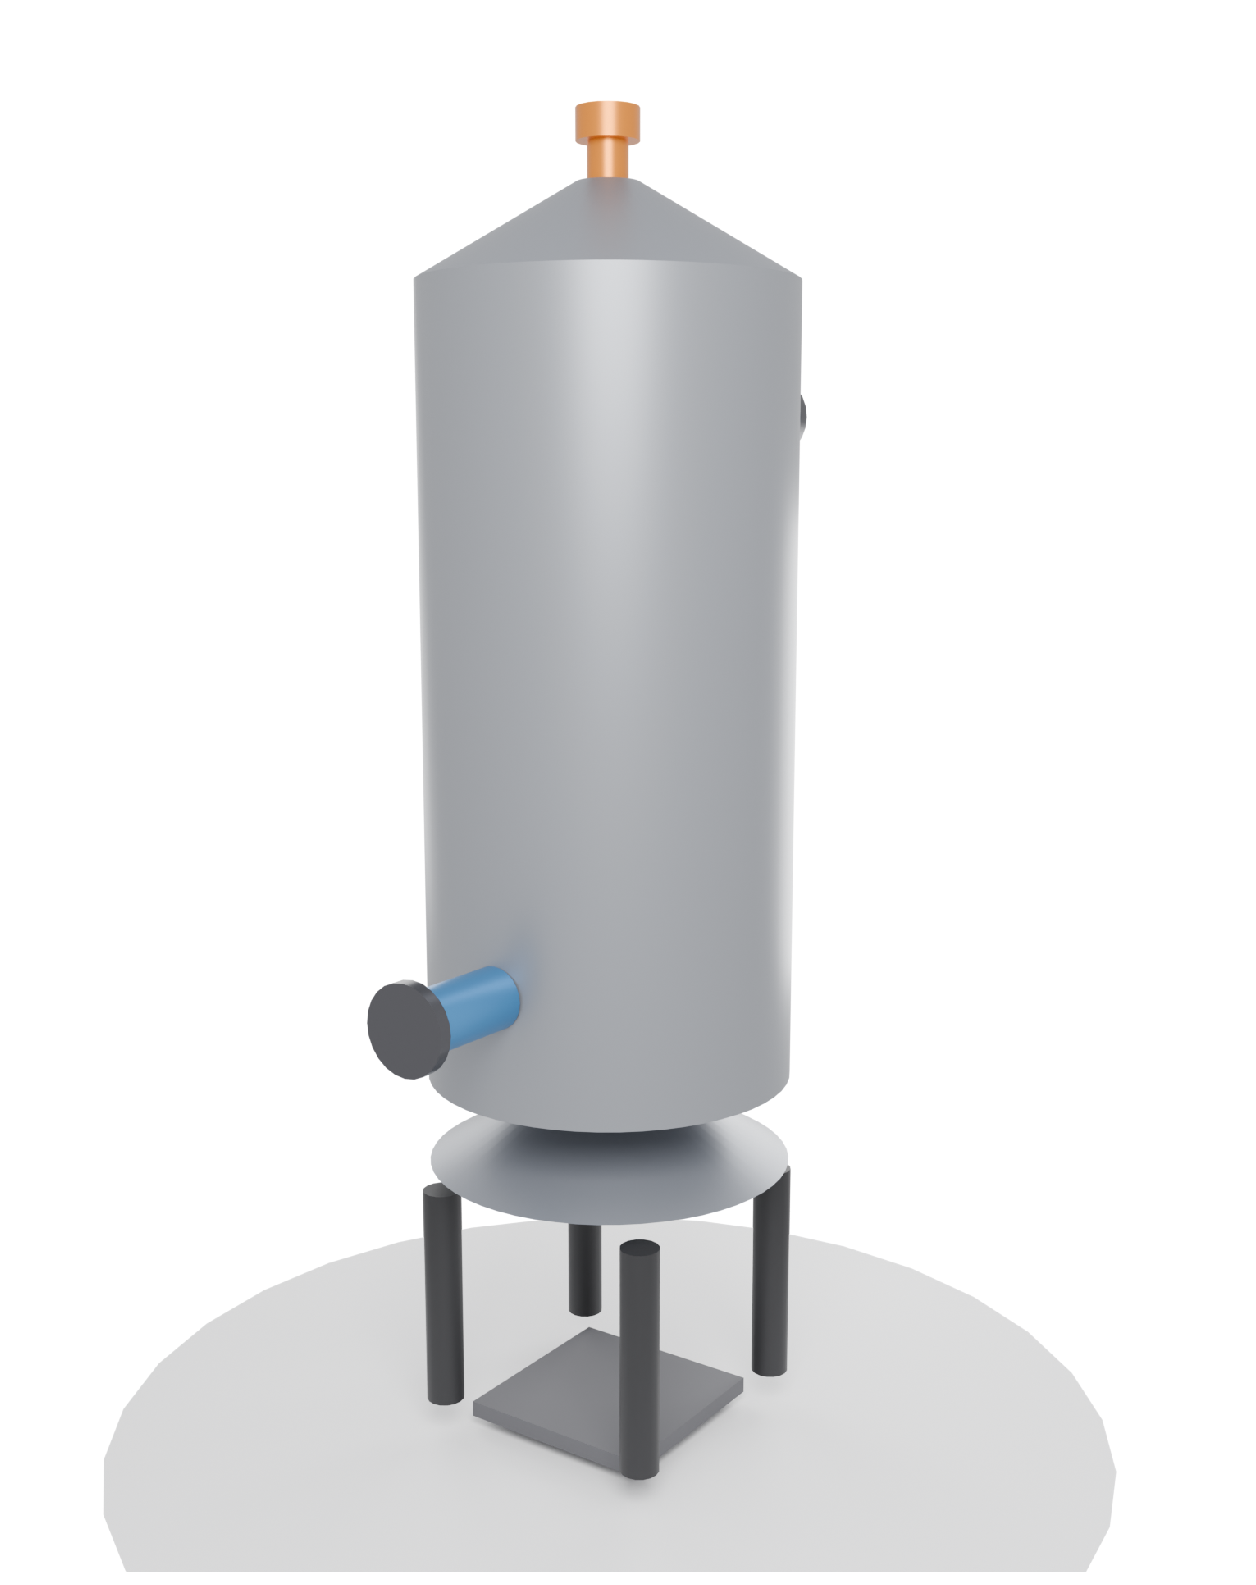
\includegraphics[width=0.48\textwidth]{figuras/fig_16_1_vaso_pulmao.pdf}
	\caption[Vaso pulmão vertical (\textit{air receiver})]{Vaso pulmão vertical (\textit{air receiver}), em perspectiva 3D — casco, cabeças toriesféricas, pernas de apoio, bocais de entrada/saída, PSV e dreno. Esquema ilustrativo, não um desenho de projeto.}
	\label{fig:16-1}
\end{figure}

\subsection{Dinâmica de Fluxo e Header de Distribuição Setorizada}

O header principal ramifica-se em três linhas com prioridades distintas. O Gêmeo Digital monitora a pressão no vaso pulmão ($P_{tank}$) e comanda válvulas de isolamento automáticas baseadas em setpoints de segurança:

\begin{itemize}
	\item \textbf{Linha de Emergência (Instrumentação):} Prioridade Máxima. Alimenta sistemas de segurança e válvulas ESD. É a última linha a ser isolada para garantir a integridade da planta.
	\item \textbf{Linha de Processo:} Prioridade Média. Alimenta a produção e extração. É isolada quando a pressão atinge o nível de alerta crítico para preservar o inventário.
	\item \textbf{Linha de Serviços (Utilidades):} Prioridade Baixa. Alimenta ferramentas pneumáticas e limpeza. É a primeira linha a sofrer restrição (\textit{load shedding}).
	\item \textbf{Balanço de Massa com Variáveis de Estado ($\delta$):} A vazão total da frota se reparte entre as três linhas de prioridade conforme o estado das válvulas de isolamento, pela Equação~\eqref{eq:s16-1}:
	\begin{equation}\label{eq:s16-1}
\dot{m}_{total} = \sum_{i=1}^{N_{\text{frota}}} \dot{m}_{comp,i} = \dot{m}_{emerg} + \delta_{proc} \cdotp \dot{m}_{proc} + \delta_{serv} \cdotp \dot{m}_{serv}
\end{equation}
	Onde $N_{\text{frota}}$ é o número de compressores ativos na frota (subscrito para não colidir com $N_{\text{rot}}$, rotação em RPM nos capítulos de rolamentos) e $\delta \in \{0, 1\}$ representa o estado (aberto/fechado) da válvula de isolamento de cada ramal.
\end{itemize}

\subsection{Pulsação de Pressão e Ressonância Acústica na Tubulação}
O balanço de massa da Equação~\eqref{eq:s16-1} descreve o nível médio de pressão no header, mas não captura as flutuações de alta frequência geradas pela passagem dos lóbulos do rotor ($f_{bp}$, Equação~\eqref{eq:s9-8}) e pelo engrenamento (GMF). Em compressores de deslocamento positivo, essas pulsações se propagam pela tubulação de descarga e podem excitar um modo acústico do sistema vaso-tubulação, risco não coberto pelo balanço de massa quase-estático já modelado.
\begin{itemize}
	\item \textbf{Frequência Acústica Natural (Ressonador de Helmholtz):} O trecho de tubulação conectando o compressor ao vaso pulmão se comporta como um ressonador de Helmholtz, cuja frequência natural é dada pela Equação~\eqref{eq:s16-2}:
	\begin{equation}\label{eq:s16-2}
 f_H = \frac{a}{2\pi} \sqrt{\frac{A_{\text{tubo}}}{V_{\text{tank}} \cdot L_{\text{eff}}}}
\end{equation}
	Onde $a$ é a velocidade do som no ar comprimido (mesmo símbolo já estabelecido na Equação~\eqref{eq:s9-13}, $a=\sqrt{\gamma R T}$, função de $T$ e da umidade), $A_{\text{tubo}}$ a área da seção do tubo, $V_{\text{tank}}$ o volume do vaso pulmão e $L_{\text{eff}}$ o comprimento efetivo do trecho (comprimento físico acrescido de correção de extremidade).
	\item \textbf{Critério de Risco de Ressonância:} O Gêmeo Digital compara $f_H$ com as frequências de excitação mecânica conhecidas do trem de compressão, pelo critério da Equação~\eqref{eq:s16-3}:
	\begin{equation}\label{eq:s16-3}
 \text{Risco de Ressonância se} \quad \left| \frac{f_H - f_{bp}}{f_H} \right| < 0.10 \quad \text{ou} \quad \left| \frac{f_H - GMF}{f_H} \right| < 0.10 
\end{equation}
	seguindo a mesma lógica de margem de separação usada na análise rotordinâmica dos eixos (Equação~\eqref{eq:s8-6}, Capítulo de Dinâmica de Transmissão), mas aplicada ao domínio acústico da tubulação, conforme a prática de projeto da API 618 \cite{api618}.
	\item \textbf{Consequência Operacional:} Ressonância sustentada amplifica a amplitude de pulsação na linha, acelerando fadiga em conexões soldadas e instrumentação de pressão, e pode ser confundida em campo com falha mecânica do próprio compressor — daí a necessidade de o modelo distinguir explicitamente pulsação acústica de vibração de origem mecânica.
	\item \textbf{Mitigação de Projeto:} Quando o critério da Equação~\eqref{eq:s16-3} indica risco, a resposta não é apenas operacional — a mesma prática da API 618 \cite{api618} que fundamenta o critério de risco trata do acessório físico correspondente: um amortecedor de pulsação (\textit{volume bottle}), instalado o mais próximo possível da descarga do compressor, que desloca $f_H$ deliberadamente para fora da faixa de excitação ao alterar o volume efetivo $V_{\text{tank}}$ e o comprimento $L_{\text{eff}}$ da Equação~\eqref{eq:s16-2}. É uma decisão de projeto, não de operação — mas o Gêmeo Digital deve registrar sua presença (ou ausência) como parâmetro fixo do sistema ao avaliar a Equação~\eqref{eq:s16-3} para cada unidade da frota.
\end{itemize}

\subsection{Lógica Escalonada de Alarmes e Proteção}

O Gêmeo Digital atua preventivamente, escalonando ações conforme a pressão do vaso pulmão declina devido a falhas na geração ou demanda excessiva:

\begin{itemize}
	\item \textbf{Nível 1 (Alerta de Pressão Baixa - $P_{L}$):} Disparo de alarme visual/sonoro e verificação automática do status de partida dos compressores em \textit{standby}.
	\item \textbf{Nível 2 (Corte de Serviços - $P_{LL}$):} Fechamento automático da válvula da Linha de Serviços ($\delta_{serv} = 0$) para estancar a queda de pressão.
	\item \textbf{Nível 3 (Corte de Processo - $P_{LLL}$):} Fechamento da válvula da Linha de Processo ($\delta_{proc} = 0$). O inventário de ar restante é dedicado exclusivamente à Emergência.
	\item \textbf{Nível 4 (Trip de Emergência - $P_{ESD}$):} Atingimento da pressão mínima de segurança para instrumentação, disparando o ESD (\textit{Emergency Shutdown}) da planta.
\end{itemize}

\subsection{Modelagem Termodinâmica Transiente e Integridade Estrutural (ASME VIII Div. 1)}

\begin{itemize}
	\item \textbf{Taxa de Variação de Pressão ($\frac{dP}{dt}$):}
	Calculada em tempo real pela Equação~\eqref{eq:s16-4} para prever a resposta do vaso pulmão frente a perturbações de demanda e modulação de compressores:
	\begin{equation}\label{eq:s16-4}
\frac{dP_{\text{vaso}}}{dt} = \frac{R \cdotp T}{V_{\text{tank}}} \cdotp \left( \sum \dot{m}_{\text{in}}(t) - \sum \dot{m}_{\text{out}}(t) \right)
\end{equation}
	\item \textbf{Integração Numérica e Parâmetros Temporais ($T_{\text{sim}}$, $\Delta t$):}
	A evolução contínua da pressão é resolvida por integração explícita de passo fixo:
	\begin{equation}\label{eq:s16-4b}
P_{\text{vaso}}(t + \Delta t) = P_{\text{vaso}}(t) + \Delta t \cdot \frac{R \cdot T}{V_{\text{tank}}} \left( \dot{m}_{\text{comp}}(t) - \dot{m}_{\text{dem}}(t) \right)
\end{equation}
	onde $\Delta t$ é o passo de amostragem/integração (tipicamente entre $0.1\text{ s}$ e $2.0\text{ s}$) e $T_{\text{sim}}$ é o horizonte temporal de análise ($10$ a $120\text{ minutos}$), acumulando $N = \frac{T_{\text{sim}} \times 60}{\Delta t}$ passos de discretização.
	\item \textbf{Limites de Integridade Estrutural (ASME Seção VIII Div. 1):}
	O Gêmeo Digital rastreia continuamente a proximidade com os limites normativos:
	\begin{enumerate}
		\item \textbf{PMTA (Pressão Máxima de Trabalho Admissível):} Limite superior de projeto do casco e cabeças ($P_{\text{PMTA}} = 10.0\text{ bar abs}$). Caso $P_{\text{vaso}} \ge P_{\text{PMTA}}$, a válvula de alívio e segurança (PSV) é acionada e o status entra em estado crítico.
		\item \textbf{Pressão Mínima Crítica de Rede ($P_{\text{mín}}$):} Limite operacional mínimo ($P_{\text{mín}} = 6.0\text{ bar abs}$) necessário para garantir o curso dos atuadores pneumáticos e sistemas de controle offshore.
		\item \textbf{Taxa Máxima Admissível de Variação ($|dP/dt|_{\text{máx}}$):} Gradientes severos ($> 1.5\text{ bar/min}$) induzem fadiga cíclica de baixo ciclo nas soldas do vaso e conexões dos bocais, sendo computados pelo gêmeo para cálculo de vida em fadiga.
	\end{enumerate}
	\item \textbf{Tempo de Autonomia por Setor ($t_{to\_cut}$):}
	Predição do tempo restante, pela Equação~\eqref{eq:s16-5}, antes que o sistema atinja o próximo nível de corte em cenário de perda de geração:
	\begin{equation}\label{eq:s16-5}
t_{to\_cut} = \frac{V_{tank} \cdotp (P_{actual} - P_{threshold})}{\dot{V}_{demand} \cdotp P_{atm}}
\end{equation}
\end{itemize}

\subsection{Matriz de Diagnóstico de Falhas (Frota e Distribuição)}

A operação com múltiplos compressores em paralelo introduz riscos específicos de frota (refluxo, sobrepressão por travamento de PSV, falha de sequenciamento) que a Tabela~\ref{tab:16-1} resume junto ao indicador primário e à ação correspondente do Gêmeo Digital.
\begin{table}[h!tbp]
\centering
\noindent\resizebox{\textwidth}{!}{
	\begin{tabular}{l l l l}
		\toprule
		\textbf{Falha} & \textbf{Indicador Primário} & \textbf{Causa Provável} & \textbf{Ação Digital Twin} \\ \midrule
		\textbf{PSV Travada (Fechada)} & $P > P_{set}$ sem alívio & Corrosão / Travamento & Trip de Emergência da Frota \\
		\textbf{Falha de Sequenciamento} & $\downarrow P_{tank}$ (Standby ativo) & Erro de lógica / Partida falha & Comando forçado de partida \\
		\textbf{Vazamento Crítico} & $\frac{dP}{dt} \ll 0$ (Gradiente alto) & Ruptura de linha principal & Antecipação do corte de ramais \\
		\textbf{Falha na Check Valve} & $\dot{m}_i < 0$ (Refluxo) & Quebra da portinhola & Isolamento da Unidade $i$ \\
		\textbf{PSV Travada (Aberta)} & Disparo prematuro & Fadiga da mola / Sujeira & Alarme de perda de eficiência \\ \bottomrule
	\end{tabular}
}
\caption[Matriz de diagnóstico de falhas de frota e distribuição]{Matriz de diagnóstico de falhas de frota e distribuição (header e vasos pulmão).}
\label{tab:16-1}
\end{table}

\subsection{Indicadores Globais de Performance (KPIs)}

\begin{itemize}
	\item \textbf{Índice de Confiabilidade de Pressão ($R_p$):} Porcentagem do tempo de operação em que $P_{tank} > P_{LL}$.
	\item \textbf{Eficiência de Resposta de Carga ($E_{resp}$):} Tempo decorrido entre a detecção da queda de pressão e a efetivação do corte do ramal.
	\item \textbf{Consumo Específico da Frota ($SPC_{fleet}$):} Cada $\dot{V}_{free\_air,i}$ é a vazão da unidade $i$ já convertida às condições de referência da Equação~\eqref{eq:s11-12} — sem essa normalização por máquina, a soma da frota misturaria vazões medidas em condições de sucção potencialmente distintas entre unidades, como soma a Equação~\eqref{eq:s16-6}:
	\begin{equation}\label{eq:s16-6}
SPC_{fleet} = \frac{\sum_{i=1}^{N_{\text{frota}}} \dot{W}_{tot,i}}{\sum_{i=1}^{N_{\text{frota}}} \dot{V}_{free\_air,i}} \quad [\text{kW} \cdotp \text{s} \cdotp \text{m}^{-3}]
\end{equation}
\end{itemize}

\vspace{1em}
\hrule
\vspace{1em}

\textbf{Diretriz Técnica Final:} A integridade do sistema depende da correta calibração dos níveis de alarme e da resposta das válvulas de isolamento. A falha da PSV em não abrir permanece como o risco mais crítico de sobrepressão, exigindo que o Gêmeo Digital monitore o gradiente positivo de pressão em relação à capacidade de alívio nominal, pela Equação~\eqref{eq:s16-7}:

\begin{equation}\label{eq:s16-7}
\boxed{\dot{m}_{leak} = \frac{V_{tank}}{R \cdotp T} \cdotp \left( \frac{dP}{dt} \right)_{static}}
\end{equation}



\clearpage
\section{Modelagem Digital Twin: IA, Exergia e Sustentabilidade}

A modelagem do Gêmeo Digital consolida o fluxo de dados massivo proveniente da rede de automação e do PI System, integrando variáveis críticas de processo com algoritmos de Inteligência Artificial e termodinâmica de segunda lei. O sistema monitora a performance mecânica, a qualidade do ar e o impacto ambiental em tempo real.

\subsection{Aquisição de Dados e Variáveis Críticas de Automação}

O Gêmeo Digital processa o vetor de medições $z(t)$ extraído continuamente da instrumentação de campo — não confundir com o vetor de \textbf{estado} $x$, as grandezas internas não medidas que o EKF estima a partir de $z$ (Capítulo 21): $z$ é o que o sensor entrega, $x$ é o que o modelo infere a partir dele. As variáveis fundamentais para a fidelidade do modelo e proteção dos equipamentos clientes são:

\begin{itemize}
	\item \textbf{Pressões ($P$):} Sucção, descarga de estágios e pressão no header de distribuição.
	\item \textbf{Temperaturas ($T$):} Entrada e saída de compressores e trocadores de calor.
	\item \textbf{Diferenciais de Pressão ($\Delta P$):} Queda de carga em filtros e secadores (indicadores de colmatação).
	\item \textbf{Vazão ($\dot{m}$):} Medição direta ou estimada para balanço de massa e energia.
	\item \textbf{Ponto de Orvalho ($T_{dp}$):} Variável crítica para conformidade com a classe de umidade contratada da ISO 8573-1 \cite{iso8573}, evitando condensação e corrosão nos equipamentos clientes.
	\item \textbf{Corrente e Tensão Elétricas ($I$, $V$):} Corrente de fase do motor principal (mesma leitura do ponto A da Tabela~\ref{tab:18-1}) e tensão de linha de alimentação — a via elétrica de acompanhamento de carga, complementar às grandezas termofluídicas acima.
	\item \textbf{Vetor de Entrada Global ($z$):} As variáveis acima se organizam no vetor de entrada da Equação~\eqref{eq:s17-1}:
	\begin{equation}\label{eq:s17-1}
z = [P, T, \Delta P, \dot{m}, T_{dp}, I, V]^T
\end{equation}
	Esta lista é ilustrativa das \textbf{categorias} de sinal disponíveis, não um vetor de dimensão fixa: a Parte II especializa esse mesmo $z$ genérico de duas formas concretas e distintas — sete elementos escolhidos por critério de observabilidade para o EKF (Equação~\eqref{eq:s21-2}, Capítulo 21) e as 26 variáveis monitoradas da Tabela~\ref{tab:18-1} como entrada do VAE (Capítulo 22). São vetores de tamanhos diferentes; o símbolo é o mesmo por seguir a notação padrão de cada literatura, não porque seja a mesma grandeza nos dois casos.
\end{itemize}

\subsection{IA para Detecção Prematura e Qualidade do Ar}

Utilizando redes neurais do tipo Autoencoders e LSTMs, o Gêmeo Digital identifica desvios sutis que precedem falhas operacionais ou perda de qualidade do ar (umidade excessiva).

\begin{itemize}
	\item \textbf{Erro de Reconstrução ($E_{rec}$):}
	O modelo aprende as correlações nominais entre as variáveis. Desvios em $T_{dp}$ ou $\Delta P$ geram um aumento no resíduo da Equação~\eqref{eq:s17-2}, que soma o erro quadrático de cada uma das $M$ variáveis do vetor $z$ (mesma fórmula reaparece, agora com normalização por variância, nas Equações~\eqref{eq:s20-4} e~\eqref{eq:s22-5}):
	\begin{equation}\label{eq:s17-2}
E_{rec} = \sum_{j=1}^{M} (z_j - \hat{z}_j)^2
\end{equation}
	
	\item \textbf{Predição de Breakthrough:} A IA analisa a taxa de variação $\frac{dT_{dp}}{dt}$ para antecipar a saturação do leito dessecante nos secadores PSA antes que o limite normativo seja atingido.
\end{itemize}

\subsection{Otimização de Processos via Exergia}

\textbf{Da entropia à exergia — uma explicação conceitual:} A Segunda Lei da Termodinâmica estabelece que a entropia de um sistema isolado nunca diminui: todo processo real — atrito, transferência de calor sob diferença finita de temperatura, ou um gás escoando livremente por um vazamento — gera entropia ($\dot{S}_{gen} \ge 0$), e esse aumento é irreversível, não há como ``desfazê-lo'' sem gastar ainda mais energia em outro lugar. A Primeira Lei garante que a energia total se conserva (nunca é destruída), mas a Segunda Lei revela algo que a Primeira não enxerga: a \textit{qualidade} dessa energia — sua capacidade de realizar trabalho útil — se degrada continuamente à medida que a entropia aumenta. É exatamente essa perda de qualidade, invisível para um balanço de energia comum, que a \textbf{exergia} foi criada para medir.

Formalmente, exergia é o trabalho útil máximo que poderia ser extraído de um fluxo de energia ou matéria, levando-o reversivelmente até o equilíbrio com o ambiente de referência (pressão e temperatura atmosféricas, $P_0$ e $T_0$). A energia nunca é destruída; a exergia, sim — e a quantidade destruída é diretamente proporcional à entropia gerada pelo processo, $\dot{I} = T_0 \cdot \dot{S}_{gen}$: essa é a mesma relação que abre a Equação~\eqref{eq:s17-3} logo abaixo, destruição de exergia é, literalmente, entropia gerada multiplicada pela temperatura ambiente — uma forma de converter a ``desordem'' termodinâmica (um conceito abstrato, medido em J/K) em uma grandeza concreta e comparável, medida em Watts.

\textbf{Exemplo aplicado a este documento:} um vazamento interno entre os rotores do compressor (a folga $\delta$ discutida nos capítulos anteriores) deixa o ar de alta pressão escoar para uma câmara de baixa pressão sem produzir nenhum trabalho útil. A energia contida nesse ar não desaparece — ela permanece no sistema, agora dissipada como calor e turbulência —, então um balanço de energia convencional não acusaria perda alguma. A exergia é o que revela o prejuízo real: o \textit{potencial} daquele ar pressurizado de realizar trabalho foi destruído de forma permanente, e $\dot{I}$ quantifica exatamente quantos Watts esse potencial valia. É essa mesma unidade (Watts de exergia destruída) que permite comparar, lado a lado e na mesma régua, o vazamento por folga interna, a incrustação no trocador de calor e o atrito no mancal — e assim priorizar qual intervenção realmente devolve mais eficiência à máquina.

O conceito estende a noção de ``energia disponível'' de Gibbs e Keenan, formalizada sob o termo \textit{exergia} por Zoran Rant em 1956 e consolidada como ferramenta de otimização de processos industriais nas décadas seguintes \cite{bejan}.

\begin{itemize}
	\item \textbf{Taxa de Destruição de Exergia ($\dot{I}$):} Formalizada na Equação~\eqref{eq:s17-3} como balanço de exergia entre entrada, saída e trabalho de eixo:
	\begin{equation}\label{eq:s17-3}
\dot{I} = T_0 \cdotp \dot{S}_{gen} = \dot{W}_{shaft} + \sum \dot{m}_{in} \psi_{in} - \sum \dot{m}_{out} \psi_{out}
\end{equation}
	Onde $\psi = (h - h_0) - T_0 \cdotp (s - s_0)$ é a exergia específica de fluxo — o trabalho útil máximo extraível de cada kg de fluido, definida por unidade de massa para poder ser multiplicada pela vazão $\dot{m}$ em cada termo da equação acima (notação de Kotas \cite{bejan}; usa-se $\psi$ em vez de $b$ para não colidir com a largura de dente da engrenagem, usada no modelo de Lewis, e com o expoente de Basquin, usado na Regra de Miner). $\dot{W}_{shaft}$ entra com sinal \textbf{positivo}: na convenção deste documento (trabalho consumido pelo compressor sempre positivo, mesma convenção de $\dot{W}_{LP}$, $\dot{W}_{HP}$ e $\dot{W}_{total}$), o trabalho de eixo é exergia que \textbf{entra} no volume de controle junto com o fluxo de massa de entrada — um compressor puxando ar ambiente ($\psi_{in}\approx0$) e descarregando ar comprimido ($\psi_{out}>0$) só produz $\dot{I}>0$ (consistente com a 2ª Lei) se $\dot{W}_{shaft}$ tiver o mesmo sinal dos termos de entrada, não o oposto.
	
	\item \textbf{Eficiência Exergética Global ($\eta_{ex}$):}
	O Gêmeo Digital busca maximizar este índice, definido na Equação~\eqref{eq:s17-4}, para garantir a operação próxima ao limite termodinâmico:
	\begin{equation}\label{eq:s17-4}
\eta_{ex} = 1 - \frac{\dot{I}_{comp} + \dot{I}_{cool} + \dot{I}_{dry}}{\dot{W}_{elec}}
\end{equation}
	O denominador usa $\dot{W}_{elec}$ (potência elétrica total consumida da rede), não a potência de eixo — a mesma convenção já adotada na Equação~\eqref{eq:s18-3} (onde $\eta_{ex}$ reaparece) e no cálculo de emissões de CO$_2$: para um índice \textbf{global} de eficiência exergética, a referência é o que a planta efetivamente consome da fonte primária, não uma potência intermediária do trem mecânico.
\end{itemize}

\subsection{Redução de Consumo e Emissões de GEE}

A redução das emissões de Gases de Efeito Estufa (GEE) é tratada como uma consequência direta da eficiência exergética. O sistema executa uma otimização multiobjetivo para equilibrar performance e sustentabilidade.

\begin{itemize}
	\item \textbf{Taxa de Emissão de $CO_2$ ($\dot{m}_{CO_2}$):} A Equação~\eqref{eq:s17-5} converte a potência elétrica total consumida pelo sistema em massa de $CO_2$ emitida, multiplicando pelo fator de emissão da matriz elétrica local ($EF_{carbon}$, em kg de $CO_2$ por kWh) — quanto mais exergia é destruída (mais potência é necessária para o mesmo trabalho útil), maior essa emissão:
	\begin{equation}\label{eq:s17-5}
\dot{m}_{CO_2} = \dot{W}_{total} \cdotp EF_{carbon} \quad [\text{kg} \cdotp \text{h}^{-1}]
\end{equation}
	
	\item \textbf{Função de Custo Ambiental ($J$):}
	O sistema ajusta setpoints para minimizar $J$, definido na Equação~\eqref{eq:s17-6}:
	\begin{equation}\label{eq:s17-6}
J = w_1 \cdotp \dot{I} + w_2 \cdotp \dot{m}_{CO_2} + w_3 \cdotp (T_{dp} - T_{dp,set})^2
\end{equation}
\end{itemize}

\subsection{Matriz de Diagnóstico, Normas e Sustentabilidade}

A Tabela~\ref{tab:17-1} conecta cada variável crítica de automação ao indicador de IA correspondente, à norma ou risco associado e à ação que o Gêmeo Digital deve tomar automaticamente.
\begin{table}[h!tbp]
\centering
\noindent\resizebox{\textwidth}{!}{
	\begin{tabular}{l l l l}
		\toprule
		\textbf{Variável PI} & \textbf{Indicador IA} & \textbf{Risco / Norma} & \textbf{Ação Gêmeo Digital} \\ \midrule
		\textbf{$T_{dp}$ (Orvalho)} & $\uparrow$ Resíduo & ISO 8573-1 / Corrosão & Antecipar ciclo de secagem \\
		\textbf{$\Delta P$ Filtros} & $\uparrow E_{rec}$ & Perda de Carga & Alarme de manutenção preditiva \\
		\textbf{$P, T$ Estágio} & Desvio de Curva & $\uparrow$ Consumo / $\uparrow$ GEE & Ajuste de carga e rotação \\
		\textbf{$\dot{m}$ (Vazão)} & Balanço de Massa & Vazamento de Inventário & Localizar perda mássica \\ \bottomrule
	\end{tabular}
}
\caption[Matriz de diagnóstico e sustentabilidade do Gêmeo Digital]{Matriz de diagnóstico, normas associadas e ações de sustentabilidade do Gêmeo Digital.}
\label{tab:17-1}
\end{table}

\vspace{1em}
\hrule
\vspace{1em}

\textbf{Diretriz Técnica Final:} A integração do ponto de orvalho como variável crítica garante a proteção dos equipamentos clientes e o atendimento às normas internacionais. O Gêmeo Digital opera no Ponto de Máxima Sustentabilidade, onde a redução de emissões é alcançada pela minimização da geração de entropia, condição formalizada na Equação~\eqref{eq:s17-7}:

\begin{equation}\label{eq:s17-7}
\boxed{\text{Min } \dot{S}_{gen} \implies \text{Min } \dot{m}_{CO_2} \quad \text{com } T_{dp} < T_{dp,limit}}
\end{equation}




\clearpage
\section{Unificação do Modelo Matemático e Matriz Global de Variáveis}

Este capítulo estabelece a síntese definitiva do Gêmeo Digital, integrando a totalidade das equações físicas, modelos estocásticos e algoritmos de inteligência artificial desenvolvidos ao longo deste estudo. A unificação abrange o fluxo completo de energia e massa, desde o relé de proteção no MCC até o header de distribuição final, consolidando a governança de dados para integridade mecânica, eficiência exergética e conformidade normativa.

\subsection{Matriz Abrangente de Variáveis, Localização e Instrumentação}

A observabilidade total do sistema — condição necessária para que o Filtro de Kalman Estendido do Capítulo 21 consiga estimar o estado interno da máquina — é garantida pelo monitoramento combinado de variáveis \textbf{reais}, lidas diretamente de um sensor físico, e \textbf{virtuais} (\textit{soft-sensors}), calculadas pelo modelo a partir das primeiras. A Tabela~\ref{tab:18-1} consolida esse mapeamento completo em seis colunas: o \textbf{ponto} de instalação (rotulado de A a I ao longo do trem de compressão, do MCC ao \textit{header} de distribuição), o \textbf{subsistema} correspondente, a \textbf{grandeza} monitorada, o \textbf{símbolo} usado no equacionamento deste documento, a \textbf{unidade} SI adotada e a \textbf{função} daquela medição no diagnóstico. Antes da tabela em si, a Figura~\ref{fig:18-1} localiza esses nove pontos na própria ordem física do trem — do MCC/relé (A) ao \textit{header} (I) —, com os principais símbolos de cada ponto, para orientar a leitura detalhada que segue.

\begin{figure}[h!tbp]
	\centering
	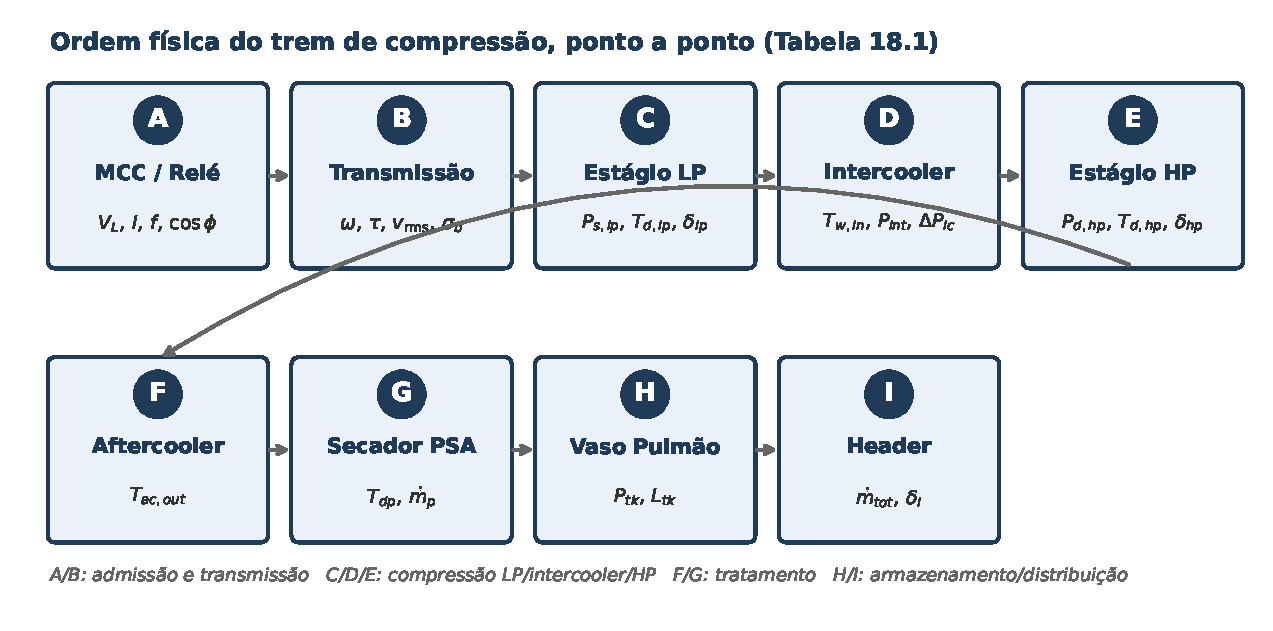
\includegraphics[width=0.80\textwidth]{figuras/fig_18_1_instrumentacao.pdf}
	\caption[Localização dos pontos de instrumentação A-I]{Localização dos nove pontos de instrumentação (A-I) ao longo da ordem física do trem de compressão, com os principais símbolos monitorados em cada um.}
	\label{fig:18-1}
\end{figure}

Duas leituras dessa tabela são úteis. Na horizontal, ela funciona como especificação de instrumentação: cada linha corresponde a um requisito de projeto verificável na lista de instrumentos da planta. Na vertical, agrupada por ponto, ela revela a densidade de medição de cada subsistema — e é aí que se identificam as lacunas de observabilidade, isto é, os pontos onde o Gêmeo Digital depende inteiramente de inferência por modelo porque não há sensor físico disponível. Essas lacunas não são falhas de projeto: instrumentar diretamente a câmara de compressão de um rotor girando a milhares de RPM é impraticável, e é justamente por isso que o \textit{soft-sensor} existe. Mas elas precisam estar explícitas, porque determinam onde a incerteza do modelo (Capítulo 25) é maior e onde a validação física do PIML (Capítulo 23) é mais crítica.

\begin{table}[h!tbp]
	\centering
	\resizebox{\textwidth}{!}{
		\begin{tabular}{c l l c l l}
			\toprule
			\textbf{Ponto} & \textbf{Localização} & \textbf{Variável} & \textbf{Tag} & \textbf{Unidade} & \textbf{Definição / Função} \\ \midrule
			\textbf{A} & \textbf{MCC / Relé} & Tensão de Linha & $V_L$ & $\text{V}$ & Potencial elétrico de alimentação \\ \cline{3-6} 
			& & Corrente de Fase & $I$ & $\text{A}$ & Carga elétrica do motor principal \\ \cline{3-6} 
			& & Frequência & $f$ & $\text{Hz}$ & Ciclo da rede / Velocidade do VFD \\ \cline{3-6} 
			& & Fator de Potência & $\cos \phi$ & $-$ & Eficiência da conversão elétrica \\
			\textbf{B} & \textbf{Transmissão} & Velocidade Angular & $\omega$ & $\text{rad}\,\cdotp\,\text{s}^{-1}$ & Rotação real do eixo primário \\ \cline{3-6} 
			& & Torque no Eixo & $\tau$ & $\text{N}\,\cdotp\,\text{m}$ & Momento torsor transmitido \\ \cline{3-6} 
			& & Vibração Global & $v_{\text{rms}}$ & $\text{mm}\,\cdotp\,\text{s}^{-1}$ & Severidade vibratória (base API 619/OEM) \\ \cline{3-6}
			& & Tensão no Dente & $\sigma_b$ & $\text{MPa}$ & Esforço na raiz da engrenagem \\
			\textbf{C} & \textbf{Estágio LP} & Pressão Sucção & $P_{s,lp}$ & $\text{bar}$ & Pressão de entrada (atmosférica) \\ \cline{3-6} 
			& & Temp. Descarga & $T_{d,lp}$ & $^{\circ}\text{C}$ & Calor de compressão do 1º estágio \\ \cline{3-6} 
			& & Folga Interna & $\delta_{lp}$ & $\mu\text{m}$ & Espaço residual entre parafusos \\
			\textbf{D} & \textbf{Intercooler} & Temp. Água In & $T_{w,in}$ & $^{\circ}\text{C}$ & Temperatura do fluido de resfriamento \\ \cline{3-6}
			& & Pressão Interestágio & $P_{int}$ & $\text{bar}$ & Sucção HP / referência da Eq.~5.14 \\ \cline{3-6}
			& & Delta Pressão & $\Delta P_{ic}$ & $\text{bar}$ & Perda de carga no trocador \\ \cline{3-6}
			& & Vazão Condensado & $\dot{m}_{c}$ & $\text{kg}\,\cdotp\,\text{h}^{-1}$ & Taxa de remoção de umidade \\
			\textbf{E} & \textbf{Estágio HP} & Pressão Descarga & $P_{d,hp}$ & $\text{bar}$ & Pressão final de compressão \\ \cline{3-6}
			& & Temp. Descarga & $T_{d,hp}$ & $^{\circ}\text{C}$ & Temperatura crítica do 2º estágio \\ \cline{3-6}
			& & Folga Interna & $\delta_{hp}$ & $\mu\text{m}$ & Desgaste/Dilatação térmica HP \\ \cline{3-6}
			& & Posição Axial & $\delta_{ax}$ & $\mu\text{m}$ & Desgaste do mancal de escora, precede vibração \\
			\textbf{F} & \textbf{Aftercooler} & Temp. Saída & $T_{ac,out}$ & $^{\circ}\text{C}$ & Temperatura pré-secagem \\
			\textbf{G} & \textbf{Secador PSA} & Ponto de Orvalho & $T_{dp}$ & $^{\circ}\text{C}$ & Umidade residual (ISO 8573-1) \\ \cline{3-6} 
			& & Vazão de Purga & $\dot{m}_{p}$ & $\text{kg}\,\cdotp\,\text{s}^{-1}$ & Ar perdido na regeneração \\
			\textbf{H} & \textbf{Vaso Pulmão} & Pressão Vaso & $P_{tk}$ & $\text{bar}$ & Energia potencial acumulada \\ \cline{3-6} 
			& & Nível Condensado & $L_{tk}$ & $\%$ & Acúmulo de líquido no pulmão \\
			\textbf{I} & \textbf{Header} & Vazão de Demanda & $\dot{m}_{tot}$ & $\text{kg}\,\cdotp\,\text{s}^{-1}$ & Consumo real da unidade offshore \\ \cline{3-6} 
			& & Status Ramal & $\delta_{i}$ & $\text{bin}$ & Lógica de corte (Serviço/Processo) \\ \bottomrule
		\end{tabular}
	}
	\caption[Matriz de variáveis e instrumentação do Gêmeo Digital]{Matriz completa de variáveis e instrumentação do Gêmeo Digital.}
	\label{tab:18-1}
\end{table}

\subsection{Consolidação do Motor de Cálculo Unificado}

O processamento matemático do Gêmeo Digital é executado através da integração de cinco domínios fundamentais, operando em tempo real sobre os dados do PI System:

\textbf{1. Domínio Eletromecânico e Fadiga Estrutural (Pontos A e B):} A Equação~\eqref{eq:s18-1} encadeia os pontos A e B da matriz acima: a potência elétrica trifásica medida no painel ($\dot{W}_{\text{elec}}$) determina o torque no eixo ($\tau_{\text{shaft}}$), que por sua vez alimenta o cálculo de tensão na raiz do dente ($\sigma_b$, mesmo modelo de Lewis da Equação~\eqref{eq:s8-7}) sob a restrição de sincronismo já vista na Equação~\eqref{eq:s8-9}:
\begin{equation}\label{eq:s18-1}
\begin{aligned}
	\dot{W}_{\text{elec}} &= \sqrt{3} \cdotp V_L \cdotp I \cdotp \cos \phi \\[8pt]
	\tau_{\text{shaft}} &= \frac{\dot{W}_{\text{elec}} \cdotp \eta_m}{\omega} \\[8pt]
	\sigma_b &= \frac{F_t}{b \cdotp m \cdotp Y} \cdotp K_v \cdotp K_o \cdotp K_s \quad \text{com} \quad \Delta \theta_{\text{sync}} < \theta_{\text{backlash}}
\end{aligned}
\end{equation}

\textbf{2. Domínio Termoflutuídico e Eficiência de Compressão (Pontos C, D e E):} A Equação~\eqref{eq:s18-2} encadeia os pontos C a E: a eficiência volumétrica ($\eta_v$, função da folga $\delta$) determina a temperatura de descarga real, e ambas alimentam o cálculo do trabalho de compressão somado sobre os dois estágios — a mesma física dos Capítulos de Termodinâmica LP e HP, agora vista como um único bloco de cálculo:
\begin{equation}\label{eq:s18-2}
\begin{aligned}
	\eta_{v} &= 1 - \frac{C_d \cdotp A_{\text{gap}}(\delta) \cdotp \sqrt{2\rho (P_d - P_s)}}{\dot{m}_{\text{th}}} \\[8pt]
	T_{\text{out}} &= T_{\text{in}} \cdotp \left( \frac{P_{\text{out}}}{P_{\text{in}}} \right)^{\frac{n-1}{n}} \\[8pt]
	\dot{W}_{\text{comp}} &= \sum_{i=1}^{2} \left[ \frac{\dot{m}_i \cdotp R \cdotp T_{s,i}}{\eta_{is,i}} \left( \frac{\gamma}{\gamma - 1} \right) \left( \left( \frac{P_{d,i}}{P_{s,i}} \right)^{\frac{\gamma-1}{\gamma}} - 1 \right) \right]
\end{aligned}
\end{equation}

\textbf{3. Domínio de Exergia e Sustentabilidade Ambiental (Global):} A Equação~\eqref{eq:s18-3} retoma a destruição de exergia introduzida na Equação~\eqref{eq:s17-3} — aqui escrita em termos de entropia de fluxo ($s$) de entrada e saída mais a troca de calor com o ambiente — e fecha a eficiência exergética global $\eta_{\text{ex}}$; a taxa de emissão de $CO_2$ (mesma forma da Equação~\eqref{eq:s17-5}) é reportada separadamente, proporcional à potência elétrica total consumida — em uma unidade offshore, cada kWh demandado dos geradores emite $CO_2$ integralmente, independentemente da eficiência exergética interna da máquina, de modo que $\eta_{\text{ex}}$ não deve descontar essa emissão:
\begin{equation}\label{eq:s18-3}
\begin{aligned}
	\dot{I} &= T_0 \left[ \sum (\dot{m}s)_{\text{out}} - \sum (\dot{m}s)_{\text{in}} - \frac{\dot{Q}}{T_{\text{surr}}} \right] \\[8pt]
	\eta_{\text{ex}} &= 1 - \frac{\dot{I}}{\dot{W}_{\text{elec}}} \\[8pt]
	\dot{m}_{\text{CO}_2} &= \dot{W}_{\text{elec}} \cdotp EF_{\text{carbon}}
\end{aligned}
\end{equation}

\textbf{4. Domínio de Qualidade do Ar e Tratamento (Pontos F e G):} A Equação~\eqref{eq:s18-4} reúne a taxa de condensação (mesma forma da Equação~\eqref{eq:s14-3}) com a degradação do coeficiente de troca térmica por incrustação (mesma relação da Equação~\eqref{eq:s10-5}) — os dois mecanismos que juntos determinam se o ar chega seco o suficiente ao secador PSA:
\begin{equation}\label{eq:s18-4}
\begin{aligned}
	\dot{m}_{\text{cond}} &= \dot{m}_a \cdotp (W_{\text{in}} - W_{\text{sat,out}}) \\[8pt]
	\epsilon_{\text{hex}} &= \frac{T_{h,in} - T_{h,out}}{T_{h,in} - T_{c,in}} \implies \frac{1}{U_{\text{real}}} = \frac{1}{U_{\text{clean}}} + R_f
\end{aligned}
\end{equation}

\textbf{5. Domínio de Dinâmica de Inventário e Autonomia (Pontos H e I):} Fechando o motor de cálculo, a Equação~\eqref{eq:s18-5} retoma a dinâmica de pressão do vaso pulmão (mesma forma da Equação~\eqref{eq:s16-4}) e a propaga para o tempo de autonomia até a pressão crítica — a última etapa antes da lógica de alarmes global apresentada a seguir:
\begin{equation}\label{eq:s18-5}
\begin{aligned}
	\frac{dP_{tk}}{dt} &= \frac{R \cdotp T}{V_{tk}} \cdotp (\dot{m}_{\text{in}} - \dot{m}_{\text{out}}) \\[8pt]
	t_{\text{hold}} &= \frac{V_{tk} \cdotp (P_{tk} - P_{\text{crit}})}{\dot{V}_{\text{demand}} \cdotp P_{\text{atm}}}
\end{aligned}
\end{equation}

\subsection{Matriz Global de Alarmes e Lógica de Decisão}

A lógica de proteção e otimização do Gêmeo Digital não se apoia em indicadores isolados, mas na correlação entre grandezas medidas diretamente por sensor e grandezas inferidas pelo modelo. A Tabela~\ref{tab:18-2} organiza essa lógica em cinco colunas: o \textbf{indicador crítico} monitorado; sua \textbf{tag} no sistema de automação; o \textbf{nível} de severidade na convenção ISA \cite{isa51} (H = alarme alto, que exige ação corretiva mas permite operação continuada; HH = desligamento por valor alto; LL = desligamento por valor baixo); a \textbf{condição de gatilho}, isto é, a inequação que o Gêmeo Digital avalia a cada ciclo de varredura; e a \textbf{ação automática} disparada. Note que os quatro primeiros indicadores são grandezas físicas medidas ou calculadas por primeiros princípios, enquanto os três últimos ($E_{\text{rec}}$, $\dot{I}$ e $\dot{m}_{\text{CO}_2}$) são indicadores virtuais que só existem porque há um modelo por trás — é essa combinação que distingue a matriz de um intertravamento convencional.

\begin{table}[h!tbp]
	\centering
	\resizebox{\textwidth}{!}{
		\begin{tabular}{l c c l l}
			\toprule
			\textbf{Indicador Crítico} & \textbf{Tag} & \textbf{Nível} & \textbf{Condição de Gatilho} & \textbf{Ação Automática} \\ \midrule
			\textbf{Ponto de Orvalho} & $T_{dp}$ & \textbf{H} & $T_{dp} > -40^{\circ}\text{C}$ (Classe 2) & Antecipar regeneração PSA / Alarme de classe ISO 8573-1 \\
			\textbf{Pressão do Vaso} & $P_{tk}$ & \textbf{LL} & $P < P_{\text{min}}$ & Corte de Linha de Serviços ($\delta_{\text{serv}}=0$) \\
			\textbf{Tensão no Dente} & $\sigma_b$ & \textbf{H} & $\sigma_b > 0.85 \sigma_{\text{adm}}$ & Limitação de torque via VFD / Unload \\
			\textbf{Vibração Global} & $v_{\text{rms}}$ & \textbf{HH} & $v_{\text{rms}} > v_{\text{trip}}$ (base da máquina) & Trip Mecânico Imediato (ESD) \\
			\textbf{Erro de Reconstrução} & $E_{\text{rec}}$ & \textbf{H} & $E > \tau_{\text{limiar}}$ & Diagnóstico de falha incipiente (Mancais) \\
			\textbf{Destruição Exergética} & $\dot{I}$ & \textbf{H} & $\uparrow$ Tendência ($+15\%$) & Ajuste de setpoint de resfriamento e purga \\
			\textbf{Emissões GEE} & $\dot{m}_{\text{CO}_2}$ & \textbf{H} & $\dot{m} > \dot{m}_{\text{target}}$ & Rebalanceamento de carga da frota \\ \bottomrule
		\end{tabular}
	}
	\caption[Matriz de decisão, alarmes e ações de controle do Gêmeo Digital]{Matriz de decisão, alarmes e ações de controle do Gêmeo Digital.}
	\label{tab:18-2}
\end{table}

Dois gatilhos da Tabela~\ref{tab:18-2} merecem qualificação normativa explícita, porque são frequentemente citados como se fossem números universais — e não são.

O primeiro é o \textbf{ponto de orvalho}. A ISO 8573-1 \cite{iso8573} não estabelece um valor único de $T_{dp}$ para ar comprimido: ela define \textit{classes de pureza}, e a classe de umidade é fixada por um ponto de orvalho sob pressão (PDP) máximo — Classe 1 para $T_{dp} \le -70\,^{\circ}$C, Classe 2 para $T_{dp} \le -40\,^{\circ}$C, Classe 3 para $T_{dp} \le -20\,^{\circ}$C, e assim por diante em direção a valores positivos. O limite de $-40\,^{\circ}$C adotado neste documento corresponde, portanto, à \textbf{Classe 2}, escolhida como requisito de projeto por ser a prática consolidada para ar de instrumentação em unidades offshore, onde a linha pode atravessar regiões não aquecidas e a margem entre o PDP e a menor temperatura de parede precisa ser generosa. Ao especificar essa restrição, o Gêmeo Digital deve registrar não só o valor, mas também o \textbf{ponto de medição} (saída do secador, a jusante do filtro de partículas) e a \textbf{pressão de referência} — um ponto de orvalho medido sob pressão de linha e outro medido após expansão à atmosfera não são a mesma grandeza, e confundi-los produz uma falsa conformidade.

O segundo é o \textbf{limiar de vibração global}. É comum encontrar o valor de $7{,}1\,\text{mm}\cdot\text{s}^{-1}$ aplicado indistintamente a qualquer máquina rotativa, por extensão da família ISO 10816/20816 \cite{iso10816, iso20816}. Essa extensão é indevida no caso presente: a ISO 20816-3 \cite{iso20816}, que substituiu a ISO 10816-3 para máquinas industriais acima de $15\,\text{kW}$, \textbf{exclui explicitamente de seu escopo os compressores rotativos de deslocamento positivo}, citando os compressores de parafuso como exemplo. A razão é física, não burocrática: a assinatura vibratória de um compressor de parafuso é dominada pela frequência de passagem de lóbulos e por pulsação de gás na descarga — componentes que elevam a vibração global sem que isso represente, por si só, degradação mecânica. Um limiar calibrado para turbomáquinas rejeitaria máquinas saudáveis e, o que é pior, poderia mascarar uma degradação real que se manifeste abaixo dele.

O critério correto para $v_{\text{trip}}$ vem de três fontes, nesta ordem de precedência: (i) o valor contratual de aceitação e alarme definido pela API 619 \cite{api619} e pelos requisitos do fabricante (OEM) para aquela carcaça específica; (ii) a \textbf{linha de base da própria máquina}, levantada no comissionamento sob condição de carga conhecida e usada como referência de tendência; e (iii) quando o componente e a montagem se enquadrarem no escopo (o motor elétrico de acionamento, por exemplo, é uma máquina industrial coberta pela ISO 20816-3), o critério da norma aplicado apenas àquele componente. Essa é, aliás, a filosofia do próprio Gêmeo Digital: o desvio relevante é o afastamento da assinatura individual da máquina, não a ultrapassagem de um número tabelado por uma norma que nunca a teve em vista.

\subsection{Sensores Portáteis e Wireless: Complemento à Instrumentação Fixa}

A Tabela~\ref{tab:18-1} assume, em todas as suas linhas, um sensor \textbf{permanentemente instalado} — cabeado até o sistema de automação, amostrando em taxa constante. Essa é a premissa correta para qualquer grandeza que alimente o intertravamento da Tabela~\ref{tab:18-2} ou o ciclo de predição-correção do EKF em tempo real (Equação~\eqref{eq:s21-4}), mas não é a única forma de instrumentação que um Gêmeo Digital pode consumir. Duas categorias de sensor \textbf{não permanente} complementam a matriz fixa sem substituí-la: o instrumento \textbf{portátil}, operado por um técnico em rondas periódicas (analisador de vibração de mão, câmera termográfica portátil, detector ultrassônico de vazamento de ar comprimido), e o nó \textbf{wireless} de retrofit — um sensor sem fio, alimentado por bateria, instalado temporária ou permanentemente num ponto que não justificava o custo de cabeamento até o painel (WirelessHART e ISA100.11a são os dois protocolos consolidados para esse retrofit industrial, ambos padronizados internacionalmente como IEC 62591 e IEC 62734 respectivamente). Ambos preenchem a mesma lacuna: pontos onde uma leitura periódica de baixo custo já entrega valor diagnóstico suficiente, sem justificar uma instalação permanente.

A Tabela~\ref{tab:18-3} lista os casos de uso mais diretos para este trem de compressão, todos complementares a um ponto já existente na Tabela~\ref{tab:18-1}, nunca substitutos de uma medição que já alimenta o intertravamento.

\begin{table}[h!tbp]
	\centering
	\resizebox{\textwidth}{!}{
		\begin{tabular}{l l l l}
			\toprule
			\textbf{Sensor} & \textbf{Ponto/grandeza complementada} & \textbf{Modo} & \textbf{Uso} \\ \midrule
			Analisador de vibração de mão & $v_{\text{rms}}$ (ponto B) & Portátil, ronda periódica & Validação cruzada do acelerômetro fixo; pontos sem acelerômetro \\
			Câmera/pistola termográfica & Carcaças, mancais, painel elétrico & Portátil, ronda periódica & Ponto quente incipiente fora da matriz fixa \\
			Detector ultrassônico de vazamento & Header e ramais (ponto I) & Portátil, ronda periódica & Perda não contabilizada em $\dot{m}_{tot}$ \\
			Contador de partículas de óleo & Circuito de lubrificação & Portátil, amostragem pontual & Complementa a série ISO 4406 já periódica (Cap. 12) \\
			Nó \textit{wireless} de vibração/temperatura & Pontos sem cabeamento viável & Wireless, retrofit & Cobertura de lacuna sem custo de cabeamento novo \\ \bottomrule
		\end{tabular}
	}
	\caption[Instrumentação portátil e wireless complementar à matriz fixa]{Instrumentação portátil e wireless complementar à matriz fixa da Tabela~\ref{tab:18-1}.}
	\label{tab:18-3}
\end{table}

O ciclo de predição-correção do EKF (Equação~\eqref{eq:s21-4}) já lida naturalmente com a irregularidade temporal dessas leituras — a etapa de predição é parametrizada pelo intervalo $\Delta t$ decorrido desde a última medição, seja ele constante (sensor fixo) ou variável (ronda semanal, nó \textit{wireless} de baixa taxa de amostragem para economizar bateria). O que o ciclo \textbf{não} ajusta sozinho é a confiança relativa depositada em cada leitura: uma medição portátil carrega ruído adicional que a fixa não tem — variabilidade de posicionamento da sonda entre rondas, ausência de um ponto de fixação calibrado, e, no caso \textit{wireless}, latência e perda ocasional de pacote. A covariância de ruído de medição $\mathcal{R}$ da Equação~\eqref{eq:s21-1} deve refletir essa diferença, inflada por um fator $\kappa_{\text{port}}$ em relação ao mesmo canal medido de forma fixa, conforme a Equação~\eqref{eq:s18-6}:

\begin{equation}\label{eq:s18-6}
\mathcal{R}_{\text{port}} = \kappa_{\text{port}} \cdot \mathcal{R}_{\text{fixo}}, \qquad \kappa_{\text{port}} > 1
\end{equation}

Ignorar essa inflação — tratar uma leitura de ronda mensal como se tivesse a mesma confiabilidade de um sensor fixo amostrado a cada segundo — tem o mesmo efeito diagnosticado pelo NIS da Equação~\eqref{eq:s21-7}: o filtro passa a confiar demais numa medição ruidosa, e a estimativa diverge da realidade de forma silenciosa, sem que nenhum alarme dispare.

\vspace{1em}
\hrule
\vspace{1em}

\textbf{Diretriz Técnica Final:} A unificação matemática, formalizada na Equação~\eqref{eq:s18-7}, permite que o Gêmeo Digital opere em um ponto de ótimo multiobjetivo, onde a segurança operacional é a restrição fundamental e a sustentabilidade é a meta de performance:

\begin{equation}\label{eq:s18-7}
\begin{aligned}
	\text{Minimizar } J &= \int_{t}^{t+\Delta t} \left( \sum \dot{I} + \beta_{\text{mpc}} \sum \dot{m}_{\text{CO}_2} \right) \, dt \\[10pt]
	\text{Sujeito a: } & \begin{cases} T_{dp} \le T_{dp,\text{limit}} \quad (\text{Qualidade}) \\ \sigma_{b} < \sigma_{\text{adm}} \quad (\text{Integridade}) \\ P_{tk} \ge P_{\text{crit}} \quad (\text{Disponibilidade}) \\ \Delta \theta_{\text{sync}} < \theta_{\text{backlash}} \quad (\text{Sincronismo}) \end{cases}
\end{aligned}
\end{equation}

A inflação de $\mathcal{R}$ da Equação~\eqref{eq:s18-6} completa essa unificação num eixo que as quatro restrições anteriores não cobrem: a \textbf{origem} do dado, não só o seu valor. Um Gêmeo Digital que trata uma leitura de ronda mensal e uma leitura de sensor fixo amostrada a cada segundo com a mesma covariância de medição está, na prática, inflando artificialmente sua própria confiança — o mesmo risco silencioso que o NIS da Equação~\eqref{eq:s21-7} existe para detectar.

\clearpage
\thispagestyle{empty}
\phantomsection
\addcontentsline{toc}{part}{Parte II --- Metodologia do Gêmeo Digital e Equacionamento Integrado}
\vspace*{\fill}
\begin{center}
	{\Huge\bfseries PARTE II}\\[2em]
	{\huge\bfseries Metodologia do Gêmeo Digital e Equacionamento Integrado}
\end{center}
\vspace*{\fill}
\clearpage

\clearpage
\section{Modelos de Solução, Acompanhamento e Redução de Dimensionalidade}

Este capítulo descreve a engenharia de integração do Gêmeo Digital, detalhando como o vasto equacionamento multidisciplinar é fundido em um motor de inferência robusto e como a complexidade de dados é tratada para diagnósticos de alta fidelidade. A abordagem proposta transcende o monitoramento convencional ao integrar modelos de primeira ordem com algoritmos de aprendizado profundo.

\subsection{Integração Híbrida: Physics-Informed Machine Learning (PIML)}

Para integrar as equações de termodinâmica, exergia e fadiga em um único modelo de solução, a abordagem adotada é o \textbf{PIML}. Diferente de modelos puramente estatísticos (caixa-preta), o PIML utiliza as leis da física como restrições fundamentais no treinamento e na execução dos algoritmos.

\begin{enumerate}
	\item \textbf{Estrutura do Modelo:}
	As equações diferenciais e algébricas (DAEs) desenvolvidas nos capítulos anteriores são incorporadas diretamente à função de perda ($Loss$) do modelo de inteligência artificial. A Equação~\eqref{eq:s19-1} soma dois termos ponderados: $L_{\text{data}}$, o erro convencional contra os dados medidos, e $L_{\text{physics}}$, a penalidade por violar as leis físicas — os pesos $\lambda_1$ e $\lambda_2$ controlam o equilíbrio entre ``confiar nos dados'' e ``confiar na física'' (mesmos símbolos usados de novo na Equação~\eqref{eq:s20-5} e simplificados a um único $\lambda$ na Equação~\eqref{eq:s23-3}, quando o termo de dados já vem normalizado por $N$ com peso implícito 1):
	\begin{equation}\label{eq:s19-1}
 L_{\text{total}} = \lambda_1 L_{\text{data}} + \lambda_2 L_{\text{physics}}
\end{equation}

	\item \textbf{Componente Físico ($L_{\text{physics}}$):}
	Este termo garante que o modelo respeite o balanço de massa e a Segunda Lei da Termodinâmica, penalizando predições que violem a conservação de energia. A Equação~\eqref{eq:s19-2} soma dois resíduos ao quadrado: o desequilíbrio entre vazão de entrada, saída e variação de massa acumulada (violação da conservação de massa), e a diferença entre o trabalho de compressão previsto e o trabalho termodinâmico teórico (violação da física do processo):
	\begin{equation}\label{eq:s19-2}
 L_{\text{physics}} = \| \dot{m}_{\text{in}} - \dot{m}_{\text{out}} - \frac{dm}{dt} \|^2 + \| \dot{W}_{\text{comp}} - \dot{W}_{\text{th}} \|^2
\end{equation}
	
	\item \textbf{Vantagem Operacional:}
	O modelo torna-se resiliente a sensores ruidosos ou falhas parciais de telemetria, pois o conhecimento físico preenche as lacunas de dados, permitindo a estimação de estados não medidos.
\end{enumerate}

\subsection{Redução de Dimensionalidade: O Modelo de Espaço Latente}

Monitorar 26 variáveis simultaneamente introduz a ``maldição da dimensionalidade'' e problemas de colinearidade. O modelo adotado para simplificar esta estrutura sem perda de informação crítica é o \textbf{Autoencoder Variacional (VAE)}.

\begin{itemize}
	\item \textbf{Limitação do PCA:} A Análise de Componentes Principais (PCA) é linear e falha ao capturar relações complexas, como a variação da viscosidade do óleo ou a dinâmica não linear da compressão politrópica.
	\item \textbf{Arquitetura do Autoencoder:}
	\begin{itemize}
		\item \textbf{Encoder ($q_{\phi}$):} Comprime o vetor de 26 variáveis ($z$) em um vetor reduzido ($\ell$) de 3 ou 4 dimensões, denominado Espaço Latente.
		\item \textbf{Bottleneck (Gargalo):} Força a rede a aprender apenas as características essenciais, ou a ``assinatura de saúde'' do compressor.
		\item \textbf{Decoder ($p_{\theta}$):} Reconstrói o vetor original ($\hat{z}$) a partir do espaço latente para validação.
	\end{itemize}
	\item \textbf{Diagnóstico por Resíduo:}
	O acompanhamento é realizado através do vetor de resíduos ($r$) — a Equação~\eqref{eq:s19-3} é simplesmente a diferença absoluta, variável por variável, entre o vetor de entrada real $z$ e a reconstrução $\hat{z}$ que o decoder produz a partir do espaço latente:
	\begin{equation}\label{eq:s19-3}
 r = | z - \hat{z} |
\end{equation}
	Se o resíduo de uma variável específica (ex: $T_{d,hp}$) cresce enquanto as outras permanecem estáveis, o Gêmeo Digital isola a falha naquele componente específico.
\end{itemize}

\subsection{Modelo de Solução: Otimização e Controle Preditivo (MPC)}

Para resolver a função objetivo multiobjetivo em tempo real, o modelo de solução utiliza o \textbf{Controle Preditivo Baseado em Modelo (MPC)} acoplado a algoritmos de otimização heurística.

\begin{enumerate}
	\item \textbf{Fluxo de Solução:}
	O Gêmeo Digital projeta o estado futuro em um horizonte de tempo $H$, buscando a combinação de rotação ($\omega$) e vazão de resfriamento que minimiza a destruição de exergia ($\dot{I}$).
	
	\item \textbf{Função Objetivo Dinâmica:} O MPC minimiza, ao longo do horizonte $H$, a função de custo da Equação~\eqref{eq:s19-4}:
	\begin{equation}\label{eq:s19-4}
 \text{Minimizar } J = \sum_{k=0}^{H} \left[ \dot{I}(k) + \beta_{\text{mpc}} \cdotp \dot{m}_{\text{CO}_2}(k) + \gamma \cdotp \Delta u(k)^2 \right]
\end{equation}
	
	\item \textbf{Restrições de Integridade:}
	A tensão calculada na raiz do dente ($\sigma_b$) atua como uma barreira de segurança: a Equação~\eqref{eq:s19-5} obriga o MPC a rejeitar qualquer solução da função objetivo da Equação~\eqref{eq:s19-4} que projete a tensão acima do limite admissível em qualquer instante $k$ do horizonte de predição — a otimização energética nunca pode violar essa restrição estrutural:
	\begin{equation}\label{eq:s19-5}
 \sigma_b(k) < \sigma_{\text{adm}} \quad \forall k \in [0, H]
\end{equation}
\end{enumerate}

\subsection{Acompanhamento de Performance e Saúde (KPIs de 3ª Geração)}

O acompanhamento evolui de simples leituras de sensores para indicadores sintéticos de alta ordem:

\begin{itemize}
	\item \textbf{Exergetic Health Index (EHI):} Mede a proximidade do sistema em relação à reversibilidade ideal, ponderado pela consistência dos dados. A Equação~\eqref{eq:s19-6} multiplica a razão entre o trabalho mínimo reversível e o trabalho real (a mesma noção de eficiência exergética da Equação~\eqref{eq:s17-4}) por um fator de desconto exponencial no erro de reconstrução do VAE — de modo que o índice só é alto quando a máquina está próxima do ideal termodinâmico \textbf{e} o modelo confia nos dados que sustentam esse cálculo:
	\begin{equation}\label{eq:s19-6}
 EHI = \frac{\dot{W}_{\text{min,rev}}}{\dot{W}_{\text{real}}} \cdotp \exp(-E_{\text{rec}})
\end{equation}
	
	\item \textbf{Remaining Useful Life (RUL) por Acúmulo de Dano (Regra de Miner):} A formulação anterior deste documento estimava o RUL como uma probabilidade adimensional $P(\text{Dano} \ge 1)$, sem unidade de tempo/ciclos e sem base física — não é derivável de nenhuma curva de fadiga real. A substituição fisicamente fundamentada usa a tensão na raiz do dente ($\sigma_b$, já calculada pelo modelo de Lewis na Equação~\eqref{eq:s8-7}, Capítulo de Dinâmica de Transmissão) como entrada de uma contagem de ciclos por \textit{rainflow} sobre o histórico de operação, convertida em dano acumulado pela Regra de Palmgren-Miner \cite{palmgren, miner}, na Equação~\eqref{eq:s19-7}:
	\begin{equation}\label{eq:s19-7}
 D = \sum_{i} \frac{n_i}{N_i(\sigma_i)} 
\end{equation}
	Onde $n_i$ é o número de ciclos observados na amplitude de tensão $\sigma_i$ e $N_i(\sigma_i)$ é o número de ciclos até a falha para essa amplitude, dado pela curva S-N de Basquin \cite{basquin} do material (ou pela curva normativa AGMA 2001 \cite{agma2001} para dentes de engrenagem), pela Equação~\eqref{eq:s19-8}:
	\begin{equation}\label{eq:s19-8}
 \sigma_i^{\,b_f} \cdot N_i = C 
\end{equation}
	com $b_f$ (expoente de Basquin, subscrito para não colidir com a largura de dente $b$ do modelo de Lewis) e $C$ constantes de fadiga do material. Falha é prevista quando $D = 1$. A Figura~\ref{fig:19-1} traça essa curva S-N em escala log-log — cada ponto vermelho representa um par $(\sigma_i, N_i)$ do histórico de ciclos por \textit{rainflow}, e é a soma das razões $n_i/N_i(\sigma_i)$ para todos esses pontos que compõe o dano $D$ da Equação~\eqref{eq:s19-7}.

	\begin{figure}[h!tbp]
		\centering
		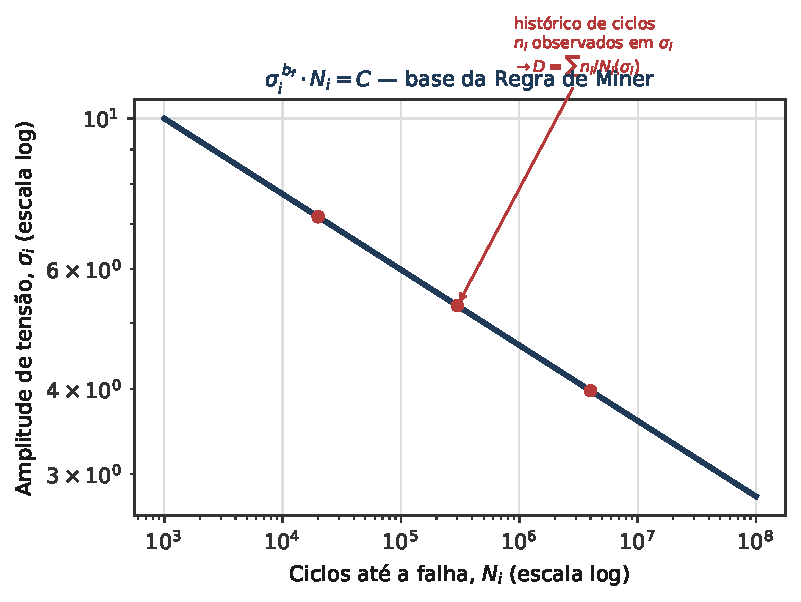
\includegraphics[width=0.60\textwidth]{figuras/fig_20_1_basquin.pdf}
		\caption[Curva S-N de Basquin]{Curva S-N de Basquin (escala log-log) — base da contagem de ciclos da Regra de Palmgren-Miner.}
		\label{fig:19-1}
	\end{figure}

	O RUL — agora expresso em ciclos ou tempo, não em probabilidade adimensional — é obtido, pela Equação~\eqref{eq:s19-9}, projetando o dano restante pela taxa de acúmulo recente $\dot{D}$, estimada a partir da janela móvel de operação:
	\begin{equation}\label{eq:s19-9}
 RUL = \frac{1 - D}{\dot{D}} 
\end{equation}
	A incerteza de $\dot{D}$ (variabilidade de carga futura, dispersão de $C$ do material) é propagada por um Processo Gaussiano (PG) ajustado sobre a série $D(t)$ estimada — um modelo bayesiano não paramétrico que, em vez de ajustar uma única curva a $D(t)$, define uma distribuição sobre todas as curvas compatíveis com o histórico observado, permitindo extrair não só a taxa média de acúmulo mas também sua variância. O PG é definido por uma função de covariância (\textit{kernel}); a mais comum é a exponencial quadrática, que codifica a suposição física central de que instantes de tempo próximos têm dano correlacionado (o dano evolui suavemente, não aos saltos). Dados os pontos já observados de $D(t)$, a média e a variância preditivas da taxa de acúmulo num instante futuro $t_*$ seguem a forma fechada de regressão por Processo Gaussiano \cite{gpml}, Equação~\eqref{eq:s19-10}:
	\begin{equation}\label{eq:s19-10}
	\begin{aligned}
		k_{\text{GP}}(t,t') &= \sigma_f^2 \exp\left( -\frac{(t-t')^2}{2\,\ell_{\text{GP}}^2} \right) \\[6pt]
		\bar{\dot{D}}(t_*) &= \mathbf{k}_{*,\text{GP}}^T \left( K_{\text{GP}} + \sigma_n^2 I \right)^{-1} \mathbf{d} \\[6pt]
		\text{Var}[\dot{D}(t_*)] &= k_{\text{GP}}(t_*,t_*) - \mathbf{k}_{*,\text{GP}}^T \left( K_{\text{GP}} + \sigma_n^2 I \right)^{-1} \mathbf{k}_{*,\text{GP}}
	\end{aligned}
	\end{equation}
	Onde $K_{\text{GP}}$ é a matriz de covariâncias entre os pontos observados de $D(t)$, $\mathbf{k}_{*,\text{GP}}$ é o vetor de covariâncias entre $t_*$ e esses pontos, $\mathbf{d}$ é o vetor das taxas de dano observadas, $\sigma_n^2$ é a variância do ruído de medição e $\ell_{\text{GP}}$ (não confundir com o vetor latente $\ell$ do VAE) é o comprimento de escala do \textit{kernel} — quanto maior, mais suave e mais correlacionada no tempo é a curva de dano assumida. A variância predita entra diretamente na Equação~\eqref{eq:s25-3} (propagação de incerteza, Capítulo de Diretrizes de Desenvolvimento) para produzir um intervalo de confiança em torno do RUL pontual da Equação~\eqref{eq:s19-9}, preservando a camada probabilística da formulação original do documento, mas agora como quantificação de incerteza em torno de um dano fisicamente calculado, e não como substituto da física.
\end{itemize}

\vspace{1em}
\hrule
\vspace{1em}

\textbf{Diretriz Técnica Final:} A solução proposta integra o rigor das equações de primeira ordem com a flexibilidade da inteligência artificial. O modelo resultante compreende a relação causal entre a degradação mecânica ($\sigma_b$) e a ineficiência térmica ($\dot{I}$), permitindo uma manutenção preditiva baseada em evidências exergéticas, consolidada na Equação~\eqref{eq:s19-11}:

\begin{equation}\label{eq:s19-11}
\boxed{\text{Min } J = \int (\dot{I} + \beta_{\text{mpc}} \dot{m}_{\text{CO}_2}) \, dt \quad \text{via PIML e Autoencoder}}
\end{equation}

	\clearpage
	\section{Fundamentos Teóricos, Algoritmos e Metodologia do Gêmeo Digital}
	
	Este capítulo estabelece a arquitetura analítica e o rigor metodológico necessários para a implementação do Gêmeo Digital (DT). A abordagem integra a mecânica clássica, a termodinâmica avançada e o aprendizado de máquina para criar um sistema de suporte à decisão prescritiva em operações offshore.
	
	\subsection{Pilares Teóricos da Modelagem Híbrida}
	
	A metodologia baseia-se no conceito de \textbf{Modelagem Gray-Box}, que funde a explicabilidade das leis físicas com a capacidade de generalização dos dados.
	
	\begin{itemize}
		\item \textbf{Estrutura de Decomposição:}
		O estado real do sistema ($y_{\text{real}}$) é modelado, pela Equação~\eqref{eq:s20-1}, como a soma de um componente determinístico e um componente estocástico de erro:
		\begin{equation}\label{eq:s20-1}
 y_{\text{real}} = f_{\text{física}}(x, \theta) + \epsilon_{\text{IA}}(x, \phi) 
\end{equation}
		\begin{itemize}
			\item $f_{\text{física}}$: Representa o conhecimento a priori (ex: equações politrópicas, balanço exergético).
			\item $\epsilon_{\text{IA}}$: Captura a deriva do modelo causada por fenômenos complexos como o desgaste de selos, incrustação (\textit{fouling}) e variações na composição do gás.
		\end{itemize}
		
		\item \textbf{Consistência Termodinâmica:}
		Diferente de modelos de IA puros, o DT é restrito pela \textbf{Segunda Lei da Termodinâmica}, garantindo, pela Equação~\eqref{eq:s20-2}, que a destruição de exergia ($\dot{I}$) seja sempre positiva:
		\begin{equation}\label{eq:s20-2}
 \dot{I} = T_0 \cdotp \dot{S}_{\text{gen}} \ge 0 
\end{equation}
	\end{itemize}
	
	\subsection{Algoritmo de Estimação de Estado: Filtro de Kalman Estendido (EKF)}
	
	O \textbf{EKF} é o algoritmo fundamental para a fusão de dados. Ele permite estimar variáveis de estado ocultas ($x$) a partir de medições ruidosas ($z$, aqui com sete elementos — definição concreta no Capítulo 21) do sistema de supervisão (PI System). O mesmo símbolo $z$ reaparece na subseção de VAE logo abaixo, mas com 26 elementos — vetor diferente, não um subconjunto deste.
	
	\begin{itemize}
		\item \textbf{Vetor de Estado ($x$):} Inclui parâmetros críticos como a folga residual ($\delta$), a eficiência isentrópica ($\eta_{\text{is}}$) e a resistência térmica de incrustação ($R_f$).
		\item \textbf{Ciclo de Predição e Correção:} A cada passo de tempo $k$, o EKF alterna entre prever o próximo estado usando o modelo físico e corrigir essa previsão contra a medição real, conforme a Equação~\eqref{eq:s20-3} — a mesma estrutura de predição-correção detalhada no Capítulo de Estimação de Estados via EKF:
	\end{itemize}
	\begin{equation}\label{eq:s20-3}
	\begin{aligned}
		\hat{x}_{k|k-1} &= f(\hat{x}_{k-1|k-1}, u_{k-1}) \\[4pt]
		P_{k|k-1} &= F_k P_{k-1|k-1} F_k^T + Q \\[4pt]
		K_k &= P_{k|k-1} G_k^T (G_k P_{k|k-1} G_k^T + \mathcal{R})^{-1} \\[4pt]
		\hat{x}_{k|k} &= \hat{x}_{k|k-1} + K_k (z_k - g(\hat{x}_{k|k-1}))
	\end{aligned}
\end{equation}
	Onde $F_k$ e $G_k$ são as matrizes Jacobianas que linearizam, respectivamente, a dinâmica do compressor ($f$) e a função de observação ($g$); $Q$ é a covariância do ruído de processo e $\mathcal{R}$ (calligráfico, para não confundir com a constante dos gases $R$ usada nos capítulos de termodinâmica) é a covariância do ruído de medição.

	\subsection{Redução de Dimensionalidade: Autoencoder Variacional (VAE)}

	Para gerenciar as 26 variáveis monitoradas, o DT utiliza o \textbf{VAE}, formalizado por Kingma e Welling em 2013 como uma extensão probabilística do autoencoder clássico \cite{vae}, para projetar os dados em um \textbf{Espaço Latente} de baixa dimensão ($\ell \in \mathbb{R}^d$, onde $d \ll 26$; usa-se $\ell$ em vez de $h$ para não colidir com a entalpia específica dos capítulos de termodinâmica).
	
	\begin{itemize}
		\item \textbf{Metodologia de Detecção de Anomalias:}
		\begin{itemize}
			\item O \textbf{Encoder} mapeia as entradas para uma distribuição de probabilidade no espaço latente.
			\item O \textbf{Decoder} reconstrói o estado nominal.
			\item O \textbf{Erro de Reconstrução} ($E_{\text{rec}}$), calculado pela Equação~\eqref{eq:s20-4} sobre as $M=26$ variáveis do vetor de entrada do VAE (aqui $z$ tem 26 elementos, não os sete do EKF da subseção anterior — mesmo símbolo, vetor diferente), atua como um sensor virtual de saúde:
		\end{itemize}
		\begin{equation}\label{eq:s20-4}
 E_{\text{rec}} = \sum_{i=1}^{M} \frac{(z_i - \hat{z}_i)^2}{\sigma_i^2} 
\end{equation}
		\begin{itemize}
			\item Se $E_{\text{rec}} > \tau$ (limiar estatístico), o algoritmo de diagnóstico é disparado para identificar qual variável causou o desvio.
		\end{itemize}
	\end{itemize}
	
	\subsection{Algoritmo Physics-Informed Machine Learning (PIML)}
	
	O \textbf{PIML} integra o equacionamento de engenharia diretamente na topologia da rede neural. A função de perda ($Loss$) é modificada para penalizar violações físicas.
	
	\begin{itemize}
		\item \textbf{Função de Perda Multiobjetivo:} Mesma estrutura já apresentada na Equação~\eqref{eq:s19-1}, agora nomeando explicitamente cada termo: erro de dados ($L_{\text{data}}$) e resíduo físico ($L_{\text{phys}}$), cada um escalado pelo seu próprio peso ($\lambda_1$, $\lambda_2$), na Equação~\eqref{eq:s20-5}:
		\begin{equation}\label{eq:s20-5}
 L = \lambda_1 \underbrace{\| y - \hat{y} \|^2}_{L_{\text{data}}} + \lambda_2 \underbrace{\| \mathcal{F}(\hat{y}) \|^2}_{L_{\text{phys}}}
\end{equation}
		Onde $\mathcal{F}(\hat{y})$ representa o resíduo das equações diferenciais, como a conservação de massa no estágio HP, na Equação~\eqref{eq:s20-6}:
		\begin{equation}\label{eq:s20-6}
 \mathcal{F} = \dot{m}_{\text{in}} - \dot{m}_{\text{out}} - \frac{d}{dt} (\rho V) 
\end{equation}
	\end{itemize}
	
	\subsection{Otimização e Tomada de Decisão: MPC e PSO}
	
	A camada superior do DT utiliza algoritmos de otimização para prescrever ações operacionais.
	
	\begin{itemize}
		\item \textbf{Controle Preditivo Baseado em Modelo (MPC):}
		O MPC resolve um problema de otimização dinâmica em um horizonte $H$, minimizando o custo operacional ($J$) da Equação~\eqref{eq:s20-7}:
		\begin{equation}\label{eq:s20-7}
 \text{Min } J = \sum_{k=0}^{H} \left[ \dot{W}_{\text{elec}}(k) + \beta_{\text{mpc}} \cdotp \dot{I}(k) \right]
\end{equation}
			Onde $\beta_{\text{mpc}}$ é subscrito para não colidir com o peso da divergência KL do VAE (Cap.~22), mesma grandeza de custo econômico-exergético já introduzida na Equação~\eqref{eq:s18-7}, aqui reaproveitada como peso do MPC.
		Sujeito às duas restrições que o otimizador nunca pode violar, independentemente do quão vantajosa a solução pareça em termos de custo: a tensão real na raiz do dente abaixo do limite admissível (integridade mecânica) e o ponto de orvalho sob pressão abaixo de $-40\,^{\circ}$C, que é o limite da \textbf{Classe 2 de umidade} da ISO 8573-1 \cite{iso8573} adotada como requisito de projeto neste documento (a norma define classes, não um valor único — ver a qualificação no Capítulo 18). Ambas são formalizadas na Equação~\eqref{eq:s20-8}:
		\begin{equation}\label{eq:s20-8}
 \begin{cases} \sigma_{b,\text{real}} < \sigma_{b,\text{adm}} \\ T_{\text{dp}} \le -40\,^{\circ}\text{C} \end{cases}
\end{equation}
		
		\item \textbf{Otimização por Enxame de Partículas (PSO):}
		Utilizado para sintonizar os hiperparâmetros do modelo e encontrar setpoints globais de resfriamento que evitem mínimos locais de eficiência.
	\end{itemize}
	
	\subsection{Metodologia de Fluxo de Trabalho (Workflow)}
	
	A implementação segue quatro etapas críticas:
	\begin{enumerate}
		\item \textbf{Ingestão e Pré-processamento:} Limpeza de dados, remoção de \textit{outliers} e sincronização temporal dos sinais de $P, T, V, I$ e vibração.
		\item \textbf{Inferência e Estimação:} Execução do EKF para determinar o estado de degradação atual e do VAE para filtrar o ruído.
		\item \textbf{Avaliação de Integridade e Exergia:} Cálculo simultâneo da tensão na raiz ($\sigma_b$) e da destruição de exergia ($\dot{I}$).
		\item \textbf{Prognóstico e Prescrição:} Estimativa da Vida Útil Remanescente (RUL) e geração de recomendações de ajuste de carga ou manutenção.
	\end{enumerate}
	
	\vspace{1em}
	\hrule
	\vspace{1em}
	
	\textbf{Diretriz Técnica Final:} A integração desses algoritmos permite que o Gêmeo Digital compreenda a \textbf{causalidade física} por trás dos dados. A metodologia garante que a otimização energética nunca comprometa a integridade estrutural, transformando o DT em um agente ativo de segurança e eficiência, síntese que a Equação~\eqref{eq:s20-9} resume.

	\begin{equation}\label{eq:s20-9}
 \boxed{y_{\text{real}} = f_{\text{física}}(x) + \epsilon_{\text{IA}}(x) \quad \text{via EKF, VAE, PIML e MPC}} 
\end{equation}


	
	\clearpage
	\section{Estimação de Estados via Filtro de Kalman Estendido (EKF)}

	Este capítulo detalha o motor de estimação de estados não observáveis, fundamental para a percepção de variáveis internas do compressor que não possuem instrumentação direta. O filtro de Kalman foi publicado por Rudolf Kalman em 1960 como solução recursiva ótima para estimação linear sob ruído gaussiano \cite{kalman}; sua extensão a sistemas não lineares (EKF), usada aqui, tornou-se padrão em estimação de estado de processos físicos desde então \cite{simon}.
	
	\subsection{Modelagem do Sistema Não Linear}
	O compressor é descrito, na Equação~\eqref{eq:s21-1}, por um sistema de equações de transição de estado ($f$) e de observação ($g$ — usa-se $g$ em vez de $h$ para não colidir com a entalpia específica dos capítulos de termodinâmica), considerando ruídos estocásticos:
	\begin{equation}\label{eq:s21-1}
	\begin{cases}
		x_k = f(x_{k-1}, u_{k-1}) + w_{k-1} \\
		z_k = g(x_k) + v_k
	\end{cases}
\end{equation}
	\begin{itemize}
		\item $x$: Vetor de estados — as grandezas internas que se deseja conhecer mas não se pode medir diretamente.
		\item $z$: Vetor de medições — o que os sensores de campo efetivamente entregam.
		\item $u$: Vetor de entradas conhecidas (comandos ao VSD, posição de válvulas), que o modelo usa para prever a evolução do estado.
		\item $w, v$: Ruídos de processo e medição com matrizes de covariância $Q$ e $\mathcal{R}$ (o $\mathcal{R}$ calligráfico distingue esta matriz da constante dos gases $R$, usada nos capítulos de termofluídica).
	\end{itemize}

	\subsection{Definição Concreta dos Vetores para o Compressor}

	A formulação da Equação~\eqref{eq:s21-1} é genérica; sua utilidade prática depende inteiramente de \textit{quais} grandezas entram em $x$ e em $z$. Essa escolha não é livre — ela é ditada pela Parte I deste documento. Os estados são exatamente as variáveis de degradação que os capítulos de mecanismos de falha identificaram como não instrumentáveis, e as medições são as grandezas que a matriz de instrumentação da Tabela~\ref{tab:18-1} confirma existirem em campo. A Equação~\eqref{eq:s21-2} formaliza essa escolha para o trem de compressão em estudo:

	\begin{equation}\label{eq:s21-2}
	x = \begin{bmatrix} \eta_{is,LP} \\ \eta_{is,HP} \\ \delta \\ R_f \\ \sigma_b \end{bmatrix}, \qquad
	z = \begin{bmatrix} P_{int} \\ T_{d,lp} \\ P_{\text{out}} \\ T_{\text{out}} \\ T_{w,\text{out}} \\ I \\ v_{\text{rms}} \end{bmatrix}, \qquad
	u = \begin{bmatrix} f_{\text{VSD}} \\ \dot{V}_{\text{demand}} \end{bmatrix}
\end{equation}

	A leitura física dessa escolha é o ponto central do capítulo. Nenhum sensor mede a folga $\delta$ entre os rotores — instrumentar diretamente uma câmara de compressão em rotação é impraticável — mas a folga governa a fuga interna e, portanto, a eficiência volumétrica, que por sua vez altera a relação entre a pressão de saída medida e a corrente elétrica consumida. O EKF explora exatamente essa cadeia causal: ele não ``mede'' a folga, ele infere qual valor de $\delta$ torna as medições observadas mais prováveis, dado o modelo físico da Parte I. O mesmo raciocínio vale para a resistência de incrustação $R_f$, inferida do descasamento entre a troca térmica prevista pela LMTD e a temperatura de água efetivamente observada na saída do trocador.

	$P_{int}$ e $T_{d,lp}$ (ponto C/D da Tabela~\ref{tab:18-1}) entram em $z$ por uma razão distinta das demais: sem eles, as duas eficiências isentrópicas $\eta_{is,LP}$ e $\eta_{is,HP}$ só deixam assinatura nas medições \textit{finais} ($P_{\text{out}}$, $T_{\text{out}}$) — e uma queda em qualquer um dos dois estágios produz um efeito quase indistinguível sobre essas mesmas duas leituras, o que degrada o condicionamento da matriz de observabilidade $\mathcal{O}$ (Equação~\eqref{eq:s21-5}) entre os dois estados. A medição intermediária quebra essa colinearidade: uma queda em $\eta_{is,LP}$ altera $T_{d,lp}$ diretamente, enquanto uma queda isolada em $\eta_{is,HP}$ não — o EKF passa a distinguir de qual estágio vem a degradação, em vez de atribuí-la de forma ambígua a ambos.

	O VAE do Capítulo 22 reaproveita o mesmo símbolo $z$ para um vetor bem maior — as 26 variáveis monitoradas da Tabela~\ref{tab:18-1}, não somente estas sete escolhidas por observabilidade. Os dois algoritmos nunca devem ser confundidos apesar do símbolo compartilhado: o EKF estima o estado dinâmico oculto $x$ a partir de um $z$ enxuto e cuidadosamente escolhido; o VAE não estima estado nenhum, apenas comprime e reconstrói um $z$ muito mais amplo para detectar desvio de padrão.

	\subsection{Linearização por Jacobianos}
	Dada a natureza não linear dos processos termofluídicos, o algoritmo realiza a linearização em cada passo de tempo. É aqui que reside a aproximação que define o EKF e o distingue do filtro de Kalman original: as funções $f$ e $g$ são substituídas pelos dois primeiros termos de suas séries de Taylor em torno da estimativa corrente, de modo que a máquina linear ótima possa ser aplicada ao sistema linearizado resultante \cite[Cap.~13]{simon}. Os Jacobianos da Equação~\eqref{eq:s21-3} são exatamente os coeficientes desse truncamento de primeira ordem, e é o descarte dos termos de ordem superior que cobra o preço discutido ao fim deste capítulo:
	\begin{equation}\label{eq:s21-3}
	F_k = \left. \frac{\partial f}{\partial x} \right|_{\hat{x}_{k-1|k-1}} \quad \text{e} \quad G_k = \left. \frac{\partial g}{\partial x} \right|_{\hat{x}_{k|k-1}}
\end{equation}

	\subsection{Ciclo de Atualização Recursiva}
	Com os Jacobianos disponíveis, o processo de estimação segue o ciclo de predição e correção na forma consagrada para o caso não linear \cite[Cap.~13]{simon}: a etapa de predição propaga estado e covariância pelo modelo físico, e a de correção pondera essa predição contra a medição recém-chegada por meio do ganho $K_k$, que é justamente a razão entre a confiança no modelo e a confiança no sensor, conforme a Equação~\eqref{eq:s21-4}:
	\begin{equation}\label{eq:s21-4}
	\begin{aligned}
		\text{Predição:} \quad \hat{x}_{k|k-1} &= f(\hat{x}_{k-1|k-1}, u_{k-1}) \\[4pt]
		P_{k|k-1} &= F_k P_{k-1|k-1} F_k^T + Q \\[8pt]
		\text{Correção:} \quad K_k &= P_{k|k-1} G_k^T (G_k P_{k|k-1} G_k^T + \mathcal{R})^{-1} \\[4pt]
		\hat{x}_{k|k} &= \hat{x}_{k|k-1} + K_k (z_k - g(\hat{x}_{k|k-1})) \\[4pt]
		P_{k|k} &= (I - K_k G_k) P_{k|k-1}
	\end{aligned}
\end{equation}

	A Figura~\ref{fig:21-1} ilustra esse ciclo ao longo de vários passos de tempo: a cada nova medição ruidosa $z_k$ (marcadores em X), a estimativa do EKF (linha azul) se aproxima do estado real não observado (linha verde), e a banda sombreada — a covariância $P_{k|k}$ da Equação~\eqref{eq:s21-4} — se estreita a cada correção, representando a redução da incerteza sobre o estado estimado.

	\begin{figure}[h!tbp]
		\centering
		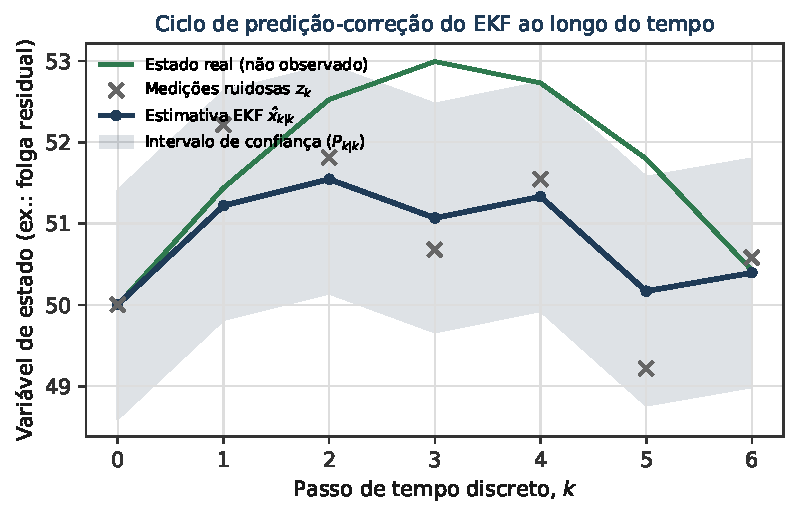
\includegraphics[width=0.60\textwidth]{figuras/fig_21_1_ekf.pdf}
		\caption[Ciclo de predição-correção do EKF]{Ciclo de predição-correção do EKF: estimativa convergindo para o estado real a partir de medições ruidosas, com banda de incerteza $P_{k|k}$.}
		\label{fig:21-1}
	\end{figure}

	\subsection{Condição de Observabilidade}

	O ciclo da Equação~\eqref{eq:s21-4} pode ser executado indefinidamente sem produzir nada de útil se o estado que se pretende estimar não deixar assinatura nas medições. Um estado \textbf{não observável} é aquele cujas variações não produzem efeito distinguível sobre $z$ — nesse caso o EKF não estima coisa alguma: ele apenas propaga a condição inicial com incerteza crescente, dando aparência de funcionamento enquanto o valor exibido no painel é ficção. Essa é a falha mais perigosa de um Gêmeo Digital, porque é silenciosa. Para o sistema linearizado a cada passo, a condição é a de posto completo da matriz de observabilidade $\mathcal{O}$, construída empilhando o Jacobiano de observação aplicado sucessivamente à dinâmica, conforme a Equação~\eqref{eq:s21-5}:

	\begin{equation}\label{eq:s21-5}
	\mathcal{O} = \begin{bmatrix} G_k \\ G_k F_k \\ G_k F_k^2 \\ \vdots \\ G_k F_k^{n_x-1} \end{bmatrix}, \qquad \text{observável} \iff \text{posto}(\mathcal{O}) = n_x
\end{equation}

	Onde $n_x$ é a dimensão do vetor de estado (cinco, no caso da Equação~\eqref{eq:s21-2}). O subscrito é necessário para não colidir com o índice politrópico $n$ dos capítulos de termodinâmica. Como $F_k$ e $G_k$ são recalculados a cada passo, a observabilidade no caso não linear é uma propriedade \textbf{local}, válida apenas na vizinhança do ponto de operação atual: um estado perfeitamente observável em plena carga pode deixar de sê-lo em carga reduzida, quando o efeito da folga $\delta$ sobre a corrente elétrica se torna pequeno demais para emergir do ruído de medição. Na prática, o Gêmeo Digital deve avaliar o número de condição de $\mathcal{O}$ em tempo de execução — mais informativo que o posto, que é uma resposta binária sobre uma matriz numérica — e sinalizar quando a estimativa de um estado específico deixou de ser sustentada pelos dados, em vez de continuar exibindo um número sem suporte na medição.

	\subsection{Inovação e Validação Estatística do Filtro}

	Existe uma grandeza que permite auditar a saúde do EKF em tempo real sem conhecer o estado verdadeiro: a \textbf{inovação}, definida como a diferença entre o que o sensor mediu e o que o modelo previa que ele mediria. Ela aparece dentro da própria etapa de correção da Equação~\eqref{eq:s21-4}, mas seu valor diagnóstico justifica tratá-la como grandeza de primeira classe, com sua covariância associada $S_k$, conforme a Equação~\eqref{eq:s21-6}:

	\begin{equation}\label{eq:s21-6}
	\tilde{z}_k = z_k - g(\hat{x}_{k|k-1}), \qquad S_k = G_k P_{k|k-1} G_k^T + \mathcal{R}
\end{equation}

	A teoria faz uma previsão forte e verificável sobre essa grandeza: se o modelo físico, as covariâncias $Q$ e $\mathcal{R}$ e as hipóteses de ruído estiverem corretos, a sequência de inovações deve ser um \textbf{ruído branco de média zero} com covariância exatamente $S_k$. Qualquer desvio desse comportamento é evidência de que alguma dessas premissas falhou. O teste padrão é a estatística NIS (\textit{Normalized Innovation Squared}), que normaliza a inovação pela incerteza esperada e cujo valor segue uma distribuição $\chi^2$ com tantos graus de liberdade quanto medições, conforme a Equação~\eqref{eq:s21-7}:

	\begin{equation}\label{eq:s21-7}
	\text{NIS}_k = \tilde{z}_k^T S_k^{-1} \tilde{z}_k \;\sim\; \chi^2_{n_z}
\end{equation}

	Onde $n_z$ é a dimensão do vetor de medições (sete aqui, Equação~\eqref{eq:s21-2}), grafada com subscrito para não colidir com o módulo de engrenagem $m$ do Capítulo 8. A interpretação operacional é direta e vale a pena explicitar, porque é ela que transforma uma identidade estatística em ferramenta de manutenção. Um NIS \textbf{consistentemente acima} da faixa esperada significa que o filtro está mais confiante do que deveria: as inovações são maiores do que $S_k$ prevê, indicando ou modelo físico defasado (a máquina degradou de um jeito que o modelo não captura) ou $Q$ subestimada. Um NIS \textbf{consistentemente abaixo} indica o contrário — covariâncias infladas, filtro excessivamente conservador, respondendo devagar demais a mudanças reais. E uma inovação com \textbf{média não nula} denuncia viés: tipicamente um sensor descalibrado ou um erro sistemático no modelo.

	Note que o NIS é calculável a cada passo sem qualquer conhecimento do estado verdadeiro. Isso o torna o único indicador realmente disponível em campo para responder à pergunta ``posso confiar nesta estimativa?'', e é a razão pela qual ele deve ser registrado e tendenciado junto com as próprias variáveis estimadas — um EKF sem monitoramento de inovação é um instrumento sem verificação de calibração.

	\subsection{Condicionamento Numérico: a Forma de Joseph}

	A atualização de covariância $P_{k|k} = (I - K_k G_k) P_{k|k-1}$, usada na Equação~\eqref{eq:s21-4} por ser a mais compacta, tem um defeito conhecido em implementações de precisão finita: ela não garante que $P$ permaneça simétrica e positiva definida. Erros de arredondamento acumulados ao longo de milhões de ciclos — e um Gêmeo Digital operando continuamente executa exatamente isso — podem tornar $P$ indefinida, momento em que o filtro diverge de forma abrupta e irrecuperável. A forma de Joseph, algebricamente equivalente mas numericamente estável por ser uma soma de dois termos estruturalmente positivos semidefinidos, é a implementação recomendada em produção, conforme a Equação~\eqref{eq:s21-8}:

	\begin{equation}\label{eq:s21-8}
	P_{k|k} = (I - K_k G_k) P_{k|k-1} (I - K_k G_k)^T + K_k \mathcal{R} K_k^T
\end{equation}

	O custo é um punhado de multiplicações matriciais adicionais por ciclo — irrelevante diante da taxa de amostragem de um compressor industrial, e barato demais para justificar o risco da forma simplificada.

	\subsection{Limites da Linearização e Alternativas}

	O EKF lineariza em torno da estimativa atual, o que embute uma hipótese: a de que a não linearidade do processo é suave o bastante para que o Jacobiano seja uma boa aproximação dentro da região de incerteza. Essa hipótese vale bem para os fenômenos térmicos e de eficiência tratados aqui, cujas curvas são monótonas e de curvatura moderada. Ela se degrada em dois cenários específicos deste equipamento: transientes rápidos de comutação das torres PSA, onde a dinâmica muda de regime em segundos, e a região próxima ao \textit{surge} ou ao travamento de válvula, onde o comportamento é fortemente não linear e a linearização local pode apontar na direção errada.

	Quando esses regimes forem relevantes para a aplicação, duas alternativas se impõem. O \textbf{Filtro de Kalman \textit{Unscented}} (UKF) substitui a linearização analítica pela propagação determinística de um conjunto de pontos amostrais (\textit{sigma points}) através da função não linear, capturando a média e a covariância com precisão de segunda ordem sem calcular Jacobianos — o que também elimina a necessidade de derivar $F_k$ e $G_k$ analiticamente, tarefa trabalhosa e propensa a erro num modelo com dezenas de acoplamentos. A \textbf{Estimação de Horizonte Móvel} (MHE), por sua vez, abandona a recursão de passo único e resolve, a cada instante, um problema de otimização sobre uma janela de medições passadas, o que permite impor \textbf{restrições explícitas} ao estado estimado — por exemplo, que a folga $\delta$ não pode ser negativa nem diminuir com o tempo, uma informação física que o EKF não tem como incorporar. Essa é precisamente a capacidade oferecida pelo \textit{framework} do-mpc discutido no Capítulo 27, e é o caminho natural de evolução deste módulo.

	\vspace{1em}
	\hrule
	\vspace{1em}

	\textbf{Diretriz Técnica Final:} O ciclo de predição-correção da Equação~\eqref{eq:s21-4} só produz estimativas confiáveis se três condições forem verificadas e monitoradas, não assumidas: observabilidade local do estado no ponto de operação corrente (Equação~\eqref{eq:s21-5}), consistência estatística da sequência de inovações via NIS (Equação~\eqref{eq:s21-7}) e estabilidade numérica da covariância via forma de Joseph (Equação~\eqref{eq:s21-8}). Matrizes $Q$ e $\mathcal{R}$ copiadas de outra instalação sem recalibração são a causa mais comum de um EKF que diverge ou passa a ignorar as medições — e o NIS é o instrumento que detecta isso antes que a estimativa errada chegue à decisão de manutenção.

	\clearpage
	\section{Redução de Dimensionalidade via Autoencoder Variacional (VAE)}
	
	A redução de dimensionalidade via VAE permite a compressão de dados complexos em assinaturas de saúde simplificadas, facilitando a detecção precoce de anomalias. A formulação usada aqui é a de Kingma e Welling \cite{vae}, que introduziu o autoencoder variacional como modelo generativo treinável por gradiente.

	\subsection{Por que um VAE, e não PCA ou um Autoencoder Simples}

	A pergunta antecede a matemática e merece resposta explícita, porque as três técnicas fazem redução de dimensionalidade e a escolha entre elas não é indiferente ao propósito de diagnóstico.

	A \textbf{Análise de Componentes Principais} (PCA) encontra a projeção linear que preserva o máximo de variância. É rápida, determinística e interpretável — mas linear. O acoplamento entre folga de rotor, temperatura de descarga e corrente elétrica neste equipamento é governado por relações politrópicas e exponenciais, mapeadas em detalhe na Parte I; forçá-las num subespaço linear descarta exatamente a estrutura que carrega a informação de degradação incipiente.

	O \textbf{autoencoder determinístico} resolve a não linearidade, mas produz um espaço latente sem estrutura garantida: nada impede que ele distribua os dados de treino arbitrariamente, com regiões vazias entre os aglomerados. Um ponto de operação novo, ainda saudável, pode cair numa dessas lacunas e gerar erro de reconstrução alto — um falso alarme.

	O \textbf{VAE} resolve os dois problemas ao impor que o espaço latente siga uma distribuição conhecida. Isso força a continuidade: pontos próximos no espaço latente decodificam para estados físicos próximos, sem lacunas arbitrárias. Para o diagnóstico, essa propriedade é o que permite interpretar a \textit{posição} no espaço latente — e não apenas o erro de reconstrução — como assinatura de saúde da máquina.
	
	\subsection{Arquitetura Probabilística e Espaço Latente}
	O VAE projeta o vetor de 26 variáveis em um espaço latente ($\ell$) modelado por distribuições gaussianas — esse vetor de entrada é chamado $z$ nas equações a seguir, com 26 elementos (Tabela~\ref{tab:18-1}); não confundir com o $z$ de sete elementos do EKF (Capítulo 21, Equação~\eqref{eq:s21-2}), símbolo compartilhado por convenção de notação, não pela mesma grandeza. A Figura~\ref{fig:22-1} ilustra essa arquitetura de ``gargalo'': o encoder comprime progressivamente a entrada $z$ até os poucos parâmetros do espaço latente, e o decoder expande esse gargalo de volta ao tamanho original, produzindo a reconstrução $\hat{z}$ — a diferença entre $z$ e $\hat{z}$ é justamente o erro de reconstrução usado como resíduo de diagnóstico mais adiante neste capítulo.

	\begin{figure}[h!tbp]
		\centering
		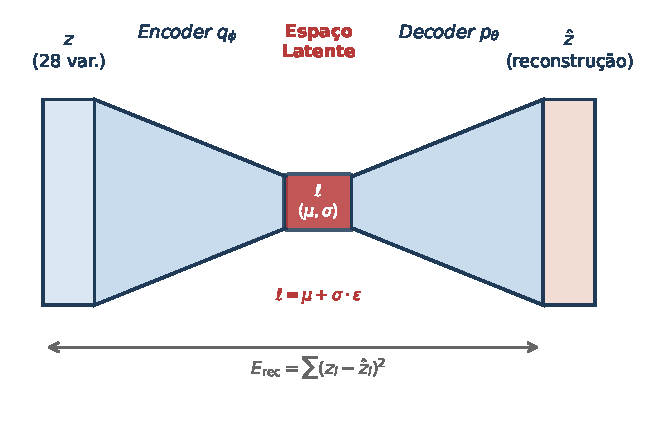
\includegraphics[width=0.75\textwidth]{figuras/fig_22_1_vae.pdf}
		\caption[Arquitetura do Autoencoder Variacional]{Arquitetura do Autoencoder Variacional: o encoder comprime o vetor de entrada $z$ até o espaço latente $\ell$ (parametrizado por $\mu$ e $\sigma$), e o decoder reconstrói $\hat{z}$ a partir dele.}
		\label{fig:22-1}
	\end{figure}

	\begin{itemize}
		\item \textbf{Encoder:} Mapeia a entrada $z$ para os parâmetros $\mu$ (média) e $\sigma$ (desvio padrão).
		\item \textbf{Reparametrização:} Para permitir a retropropagação do gradiente através de uma amostragem estocástica, o vetor latente é obtido deslocando a média por um ruído gaussiano padrão escalado pelo desvio padrão aprendido, conforme a Equação~\eqref{eq:s22-1}:
		\begin{equation}\label{eq:s22-1}
 \ell = \mu + \sigma \cdotp \epsilon, \quad \epsilon \sim \mathcal{N}(0,1)
\end{equation}
	\end{itemize}

	\subsection{Origem da Função de Perda: o Limite Inferior da Evidência}

	A função de perda do VAE não é uma combinação heurística de dois termos convenientes — ela é consequência direta de um problema de inferência bem posto, e entender essa origem é o que permite ajustá-la com critério em vez de por tentativa e erro.

	O objetivo ideal seria maximizar a verossimilhança dos dados observados, $\log p(z)$: encontrar os parâmetros de rede que tornam os dados de operação saudável os mais prováveis possíveis. O problema é que calcular $p(z)$ exige integrar sobre todas as configurações possíveis do espaço latente, uma integral intratável. A saída é introduzir uma distribuição aproximada $q(\ell|z)$ — justamente o que o encoder produz — e maximizar, em vez da verossimilhança, um limite inferior a ela. Esse limite é o ELBO (\textit{Evidence Lower Bound}), estabelecido por Kingma e Welling como objetivo diretamente treinável por gradiente \cite{vae} e formalizado na Equação~\eqref{eq:s22-2}:

	\begin{equation}\label{eq:s22-2}
	\log p(z) \;\ge\; \underbrace{\mathbb{E}_{q(\ell|z)}\left[ \log p(z|\ell) \right]}_{\text{verossimilhança da reconstrução}} \;-\; \underbrace{D_{KL}\left[ q(\ell|z) \parallel p(\ell) \right]}_{\text{afastamento da distribuição-alvo}}
\end{equation}

	Os dois termos do ELBO têm leitura direta. O primeiro pergunta: dado o código latente que o encoder gerou, quão provável é reconstruir a entrada original? Maximizá-lo é minimizar o erro de reconstrução. O segundo mede o quanto a distribuição produzida pelo encoder se afasta da distribuição-alvo $p(\ell) = \mathcal{N}(0,1)$; minimizá-lo é o que impõe a estrutura contínua no espaço latente discutida acima. Maximizar o ELBO é, portanto, exatamente equivalente a minimizar a perda da Equação~\eqref{eq:s22-3} — com o sinal trocado e com um peso $\beta$ acrescentado ao segundo termo.

	\subsection{Função de Perda e Regularização}
	Invertendo o sinal do ELBO e introduzindo o peso $\beta$, o treinamento busca o equilíbrio entre a fidelidade da reconstrução e a organização do espaço latente:
	\begin{equation}\label{eq:s22-3}
	L_{\text{VAE}} = \underbrace{\| z - \hat{z} \|^2}_{\text{Erro de Reconstrução}} + \beta \cdotp \underbrace{D_{KL} [ \mathcal{N}(\mu, \sigma) \parallel \mathcal{N}(0, 1) ]}_{\text{Divergência KL}}
\end{equation}

	O termo de divergência KL, que na forma geral exigiria integração numérica, admite \textbf{forma fechada} quando ambas as distribuições são gaussianas — que é precisamente o caso construído aqui. Essa é a razão prática de se escolher gaussianas: o gradiente sai analítico e o treinamento fica barato. Para um espaço latente de $d$ dimensões, a Equação~\eqref{eq:s22-4} dá a expressão implementada em código:

	\begin{equation}\label{eq:s22-4}
	D_{KL} = -\frac{1}{2} \sum_{j=1}^{d} \left( 1 + \log \sigma_j^2 - \mu_j^2 - \sigma_j^2 \right)
\end{equation}

	Vale notar o comportamento dessa expressão: ela se anula quando $\mu_j = 0$ e $\sigma_j = 1$ para toda dimensão $j$, e cresce conforme o encoder se afasta desse alvo. O parâmetro $\beta$ controla o quanto esse afastamento custa. Com $\beta \to 0$ o VAE degenera no autoencoder determinístico, com todas as patologias de espaço latente descritas anteriormente; com $\beta$ grande demais ocorre o \textit{posterior collapse}, em que o encoder passa a ignorar a entrada e emitir sempre $\mathcal{N}(0,1)$, produzindo reconstruções que são apenas a média dos dados de treino. Ambos os extremos destroem a capacidade de diagnóstico, e o sintoma do segundo é característico: erro de reconstrução alto e uniforme, insensível ao estado real da máquina.

	\subsection{Diagnóstico de Falhas por Resíduo}
	A saúde do sistema é monitorada pelo erro de reconstrução, já introduzido na Equação~\eqref{eq:s20-4} do Capítulo 20 e reproduzido aqui por conveniência — mesma definição, não uma segunda fórmula:
	\begin{equation}\label{eq:s22-5}
 E_{\text{rec}} = \sum_{i=1}^{M} \frac{(z_i - \hat{z}_i)^2}{\sigma_i^2}
\end{equation}
	A normalização por $\sigma_i^2$ (variância de cada variável $i$ no conjunto de treino saudável) não é opcional: o vetor de 26 variáveis monitoradas mistura grandezas de escalas completamente diferentes (pressões em bar, temperaturas em °C, vibração em mm/s) — sem normalizar, a variável de maior escala numérica dominaria a soma e mascararia desvios reais nas demais. Desvios em relação ao padrão aprendido indicam degradação mecânica ou térmica.

	\subsection{A Premissa Crítica: Pureza do Conjunto de Treinamento}

	Toda a lógica de diagnóstico acima repousa numa premissa que raramente é enunciada e frequentemente é violada: o VAE deve ser treinado \textbf{exclusivamente com dados de operação saudável}. O erro de reconstrução só funciona como indicador de anomalia porque a rede nunca aprendeu a reconstruir estados degradados — confrontada com um, ela erra, e é esse erro que denuncia a falha.

	A consequência prática é severa. Se o histórico usado no treinamento contiver períodos em que a máquina já operava com mancal degradado ou trocador incrustado, a rede aprenderá esses estados como normais e passará a reconstruí-los com erro baixo. O Gêmeo Digital ficará então estruturalmente cego justamente à falha que mais ocorreu na planta. Como raramente existe garantia de que um histórico longo seja inteiramente saudável, a curadoria do conjunto de treinamento não é etapa preliminar dispensável, e sim requisito de projeto: os períodos devem ser filtrados contra registros de manutenção, e é recomendável usar o \textit{Isolation Forest} do Capítulo 25 como triagem prévia para remover do conjunto de treino os trechos anômalos antes de treinar o VAE.

	\subsection{Definição do Limiar de Disparo}

	O erro de reconstrução da Equação~\eqref{eq:s22-5} é um número sem escala absoluta — não existe valor universal de $E_{\text{rec}}$ que signifique ``falha''. O limiar $\tau_{\text{limiar}}$ precisa ser derivado da distribuição empírica do próprio erro sobre dados saudáveis não usados no treinamento (conjunto de validação), tomando um quantil elevado como corte, conforme a Equação~\eqref{eq:s22-6}:

	\begin{equation}\label{eq:s22-6}
	\tau_{\text{limiar}} = \mathcal{Q}_{1-\alpha}\left( \{ E_{\text{rec}}^{(i)} \}_{i \in \text{validação}} \right)
\end{equation}

	Onde $\mathcal{Q}_{1-\alpha}$ é o quantil de ordem $1-\alpha$ e $\alpha$ é a taxa de falsos alarmes aceita por projeto. A escolha de $\alpha$ é uma decisão de engenharia, não estatística: $\alpha = 0{,}01$ significa aceitar que aproximadamente um a cada cem pontos saudáveis dispare alarme. Numa planta offshore com aquisição a cada segundo, isso equivale a centenas de falsos alarmes por dia — inaceitável. Por isso o disparo deve exigir \textbf{persistência}, isto é, ultrapassagem de $\tau_{\text{limiar}}$ sustentada por uma janela temporal mínima, e não um único ponto isolado.

	\subsection{O Espaço Latente como Assinatura de Saúde}

	O erro de reconstrução responde \textit{se} algo está errado, mas não \textit{o quê}. A posição no espaço latente responde à segunda pergunta, e é aqui que a estrutura contínua imposta pela divergência KL rende seu segundo dividendo. Como modos de falha distintos deslocam a máquina para regiões diferentes do espaço latente, a distância de Mahalanobis entre o código latente atual e a distribuição dos códigos saudáveis fornece um indicador direcional, conforme a Equação~\eqref{eq:s22-7}:

	\begin{equation}\label{eq:s22-7}
	d_M(\ell) = \sqrt{ (\ell - \bar{\ell}_{\text{sadio}})^T \Sigma_{\text{sadio}}^{-1} (\ell - \bar{\ell}_{\text{sadio}}) }
\end{equation}

	Onde $\bar{\ell}_{\text{sadio}}$ e $\Sigma_{\text{sadio}}$ são a média e a covariância dos códigos latentes do conjunto saudável. A utilidade operacional é que, acumulando histórico, as regiões do espaço latente podem ser \textbf{rotuladas} com os modos de falha efetivamente observados na planta — transformando o VAE de detector genérico de anomalia em classificador de causa raiz, alimentado pela mesma matriz de mecanismos de falha construída na Parte I.

	\vspace{1em}
	\hrule
	\vspace{1em}

	\textbf{Diretriz Técnica Final:} O peso $\beta$ na Equação~\eqref{eq:s22-3} controla diretamente a sensibilidade do resíduo da Equação~\eqref{eq:s22-5}: um $\beta$ alto demais organiza o espaço latente às custas da fidelidade de reconstrução, mascarando desvios reais, até o limite do \textit{posterior collapse}; um $\beta$ baixo demais devolve as patologias do autoencoder determinístico. Antes disso, porém, vale a premissa que nenhuma sintonia corrige: um VAE treinado sobre histórico contaminado com operação degradada aprende a falha como normal e fica cego a ela. Curadoria do conjunto de treinamento primeiro, sintonia de $\beta$ depois, e limiar $\tau_{\text{limiar}}$ derivado por quantil da Equação~\eqref{eq:s22-6} com exigência de persistência — nunca um valor absoluto herdado de outra instalação.

	\clearpage
	\section{Aprendizado Informado pela Física (PIML)}

	O aprendizado informado pela física garante que a inteligência artificial opere estritamente dentro dos limites impostos pelas leis termodinâmicas e mecânicas. A formulação de redes neurais informadas pela física (PINNs), que fundamenta o PIML aqui aplicado, foi sistematizada por Raissi, Perdikaris e Karniadakis em 2019 como forma de incorporar equações diferenciais diretamente na função de perda de redes neurais \cite{piml}, e consolidada como campo de pesquisa na revisão abrangente de Karniadakis e colaboradores \cite{piml2}.
	
	\subsection{Integração de Restrições Físicas}
	A rede neural é treinada para minimizar o erro dos dados enquanto satisfaz o resíduo físico $\mathcal{F}$ (mesma notação usada no Capítulo de Fundamentos Teóricos; evita-se $\mathcal{R}$ aqui para não colidir com a covariância de ruído de medição do EKF) derivado de equações diferenciais. A construção é a proposta original de Raissi, Perdikaris e Karniadakis \cite{piml}: escrever a equação diferencial governante na forma de um resíduo que deve se anular e avaliá-lo sobre a própria saída da rede, transformando a lei física em uma parcela da função de perda. A Equação~\eqref{eq:s23-1} dá essa forma genérica:
	\begin{equation}\label{eq:s23-1}
 \mathcal{F} = \frac{\partial \hat{y}}{\partial t} + \mathcal{N}_{\text{phys}}[\hat{y}] = 0
\end{equation}

	\subsection{O Operador Físico Concreto deste Compressor}

	A Equação~\eqref{eq:s23-1} é um esqueleto: o operador $\mathcal{N}_{\text{phys}}$ é abstrato até que se diga quais leis, especificamente, a rede é obrigada a respeitar. Neste documento essa resposta já existe — ela é o conteúdo inteiro da Parte I. O PIML não introduz física nova; ele apenas transporta a física já equacionada componente a componente para dentro da função de perda da rede. A Equação~\eqref{eq:s23-2} explicita os três resíduos efetivamente impostos ao modelo do trem de compressão:

	\begin{equation}\label{eq:s23-2}
	\mathcal{F} = \begin{cases}
		\mathcal{F}_1 = \dot{m}_{\text{in}} - \dot{m}_{\text{out}} - \dfrac{dm_{\text{cv}}}{dt} & \text{(conservação de massa)} \\[10pt]
		\mathcal{F}_2 = \dot{W}_{\text{elec}}\,\eta_{\text{mot}} - \dot{m}\,\Delta h - \dot{Q}_{\text{rej}} - \dfrac{dU_{\text{cv}}}{dt} & \text{(conservação de energia)} \\[10pt]
		\mathcal{F}_3 = \max\left(0,\; -\dot{S}_{gen}\right) & \text{(Segunda Lei)}
	\end{cases}
\end{equation}

	Os dois primeiros resíduos são igualdades: a rede é penalizada proporcionalmente ao quanto sua predição desequilibra o balanço de massa ou de energia do volume de controle. O terceiro é de natureza diferente e merece atenção — é uma \textbf{desigualdade}, imposta pelo operador $\max$, que só penaliza quando a taxa de geração de entropia predita é negativa. Uma rede puramente orientada a dados pode perfeitamente prever, por interpolação entre pontos de treino, uma combinação de temperaturas e pressões que corresponderia a um processo de entropia decrescente — termodinamicamente impossível, mas numericamente plausível para um interpolador. O resíduo $\mathcal{F}_3$ é a barreira que impede essa predição de sobreviver ao treinamento, e é o exemplo mais nítido de por que a Parte I precisou vir antes da Parte II.

	\subsection{Função de Perda Híbrida}
	A função de custo soma o erro nos dados observados à violação dos resíduos da Equação~\eqref{eq:s23-2}, penalizando predições que contrariem a conservação de massa, a conservação de energia ou a Segunda Lei. Essa soma de duas parcelas ponderadas — um termo supervisionado sobre pontos medidos e um termo de resíduo sobre pontos de colocação — é a forma canônica da perda de uma PINN \cite{piml}, formalizada na Equação~\eqref{eq:s23-3}, e é o que a distingue de uma rede convencional treinada apenas em dados:
	\begin{equation}\label{eq:s23-3}
 L_{\text{PIML}} = \frac{1}{N} \sum (y - \hat{y})^2 + \lambda \cdotp \frac{1}{N_f} \sum \| \mathcal{F}(\hat{y}) \|^2
\end{equation}
	Onde $\lambda$ é o peso da consistência física no aprendizado, $N$ o número de pontos de dados medidos e $N_f$ o número de pontos de colocação, definidos a seguir.

	\subsection{Pontos de Colocação e Diferenciação Automática}

	Dois detalhes de implementação distinguem uma PINN de uma rede convencional, e ambos costumam ser omitidos em descrições de alto nível — o que leva à impressão equivocada de que basta ``somar um termo físico'' à perda.

	O primeiro é como as derivadas de $\mathcal{F}$ são obtidas. Elas não são calculadas por diferenças finitas sobre uma malha, como num solver numérico clássico; são obtidas por \textbf{diferenciação automática}, o mesmo mecanismo que a biblioteca já usa para propagar gradientes no treinamento. Como a rede é uma composição de funções analíticas, $\partial \hat{y} / \partial t$ é exata até precisão de máquina, sem erro de truncamento e sem necessidade de discretizar o domínio. É essa propriedade que torna a abordagem viável.

	O segundo é onde o resíduo físico é avaliado. Os \textbf{pontos de colocação} — os $N_f$ pontos do segundo somatório da Equação~\eqref{eq:s23-3} — são posições no domínio de entrada onde se exige que a física seja satisfeita, e são \textbf{independentes dos dados medidos}. Eles não precisam de sensor algum, apenas de coordenadas. A consequência é o que dá ao PIML sua vantagem decisiva neste projeto: é possível impor conservação de energia em regiões do envelope operacional onde \textbf{nunca houve medição} — em razões de pressão que a máquina raramente atinge, em temperaturas ambientes extremas. Uma rede puramente orientada a dados extrapola nessas regiões sem qualquer garantia; a PINN ao menos extrapola sem violar as leis de conservação. Para um equipamento offshore, onde o custo de levar a máquina a condições extremas para coletar dados é proibitivo, essa é a diferença entre um modelo utilizável e um modelo restrito ao ponto de operação nominal.

	\subsection{Balanceamento Adaptativo dos Termos de Perda}

	O peso $\lambda$ fixo da Equação~\eqref{eq:s23-3} esconde um problema numérico real: os dois termos da perda têm escalas físicas completamente diferentes. Um resíduo de conservação de energia expresso em watts e um erro de temperatura expresso em kelvin diferem em ordens de grandeza, e o gradiente do termo maior domina o treinamento, tornando o outro efetivamente invisível ao otimizador. Sintonizar $\lambda$ manualmente contra esse desbalanço é trabalhoso e frágil.

	A alternativa recomendada é ajustar o peso ao longo do treinamento, em função da magnitude relativa dos gradientes de cada termo, conforme a Equação~\eqref{eq:s23-4}:

	\begin{equation}\label{eq:s23-4}
	\lambda^{(t+1)} = (1-\kappa)\,\lambda^{(t)} + \kappa \cdot \frac{\overline{\left| \nabla_\theta L_{\text{dados}} \right|}}{\overline{\left| \nabla_\theta L_{\text{física}} \right|}}
\end{equation}

	Onde $\theta$ são os parâmetros da rede, as barras indicam a média das magnitudes dos gradientes na iteração corrente e $\kappa \in (0,1)$ é um fator de suavização que evita oscilação brusca do peso. O efeito é equalizar automaticamente a influência dos dois termos sobre o passo de otimização, independentemente das unidades em que cada um foi escrito. Além disso, quando os três resíduos da Equação~\eqref{eq:s23-2} têm escalas muito distintas entre si, a prática correta é atribuir um peso próprio a cada um, em vez de um $\lambda$ único para o bloco físico inteiro.

	\subsection{Limitações e Cautelas}

	A revisão de Karniadakis e colaboradores \cite{piml2} — a mesma que consolidou o campo — é explícita quanto às suas limitações, e reproduzi-las aqui é mais honesto do que apresentar o PIML como garantia automática de validade física.

	Primeiro, e mais importante: a penalização é \textbf{fraca}, não uma restrição rígida. Minimizar $\| \mathcal{F} \|^2$ reduz a violação das leis físicas, mas não a zera. A rede treinada produz predições \textit{aproximadamente} conservativas, e a magnitude residual dessa violação precisa ser medida e reportada, não presumida desprezível. Onde a garantia precisar ser dura — numa restrição de segurança, por exemplo — a imposição deve ser feita na camada de otimização com restrições do MPC (Capítulo 24), não na perda da rede.

	Segundo, o treinamento de PINNs é notoriamente mais difícil de convergir que o de redes convencionais. O panorama de otimização é mal condicionado, e patologias de gradiente entre os termos são frequentes — daí a necessidade do balanceamento adaptativo descrito acima.

	Terceiro, o benchmarking do campo ainda é imaturo: comparações justas entre PINNs e solvers numéricos clássicos são escassas, e para problemas em que já existe um solver rápido e confiável, a PINN pode não oferecer vantagem alguma. Neste projeto a justificativa é específica e deve ser mantida à vista: substituir simulações CFD caras por um modelo substituto (\textit{surrogate model}) que responde em milissegundos, viabilizando o uso em laço de controle — e não superar o CFD em acurácia.

	\subsection{Divisão de Papéis entre PIML e EKF}

	Uma dúvida legítima surge neste ponto: se o EKF do Capítulo 21 também usa o modelo físico, e o PIML também estima grandezas não medidas, os dois não estariam fazendo a mesma coisa? Não — e a distinção esclarece a arquitetura do Gêmeo Digital.

	O EKF opera \textbf{online}, num único ponto no tempo, e responde: ``dado o modelo físico e a medição que acabou de chegar, qual o estado mais provável agora?''. Sua saída é uma estimativa com incerteza quantificada, atualizada a cada ciclo de varredura. O PIML opera \textbf{offline}, sobre todo o histórico, e responde: ``que função aproxima o comportamento desta máquina em todo o envelope operacional, inclusive onde não há dados, sem violar as leis de conservação?''. Sua saída é um modelo substituto rápido.

	Os dois se compõem em vez de competir: o modelo substituto treinado por PIML pode ser usado \textit{como} a função de transição $f(\cdot)$ do EKF, substituindo um modelo físico analítico caro de avaliar por uma rede que roda em microssegundos — o que permite ao EKF operar em taxa de amostragem alta o suficiente para capturar transientes rápidos. E o mesmo substituto serve de modelo de predição para o MPC do Capítulo 24, onde o custo de avaliação é multiplicado por todo o horizonte de otimização.

	\subsection{Identificação de Parâmetros por Problema Inverso}

	A formulação original de Raissi, Perdikaris e Karniadakis \cite{piml} cobre dois problemas com a mesma máquina matemática: o \textbf{problema direto} — conhecidos os parâmetros físicos, prever o estado — que é o que as subseções anteriores descreveram; e o \textbf{problema inverso} — conhecido o estado, a partir de medições de campo, identificar o parâmetro físico que o produziu. É a mesma pergunta que motiva a Seção~28.1 deste documento (calibração via EKF com estado aumentado), mas resolvida aqui por um mecanismo diferente, mais adequado quando o parâmetro procurado varia com a posição no domínio — não só com o tempo — ou quando não há necessidade de estimativa em tempo real, apenas uma calibração única a partir do histórico acumulado de operação.

	A diferença de formulação é pequena, mas decisiva. Em vez de tratar o parâmetro físico $\Xi$ (ex.: um coeficiente de perda, a condutância de um trocador, a rigidez de um elemento) como constante conhecida dentro do operador $\mathcal{N}_{\text{phys}}$ da Equação~\eqref{eq:s23-1}, ele passa a ser mais uma variável treinável da rede — otimizada junto com os pesos $\theta$, não fixada antes do treinamento, na Equação~\eqref{eq:s23-5}:

	\begin{equation}\label{eq:s23-5}
	\min_{\theta,\, \Xi} \; L_{\text{inv}}(\theta, \Xi) = \frac{1}{N}\sum (y-\hat{y})^2 + \lambda \cdot \frac{1}{N_f}\sum \left\| \mathcal{F}(\hat{y}; \Xi) \right\|^2
	\end{equation}

	A rede aprende simultaneamente a reproduzir os dados medidos e o valor de $\Xi$ que torna essa reprodução consistente com a física — exatamente o mecanismo que a Tabela~\ref{tab:27-1} atribui ao DeepXDE, ferramenta especializada em problemas inversos sobre equações diferenciais, na camada de \textit{PDE Solver} da arquitetura de alta performance do Capítulo 27.

	Essa técnica responde a uma limitação real deste documento: os parâmetros de catálogo usados na Parte I são valores de referência de fabricante, calibrados em condições padronizadas de bancada, e podem variar de forma sistemática de uma instalação real para outra — por qualidade de montagem, tipo de invólucro (Capítulo 2), condições ambientais do sítio ou o lote de fabricação do componente. Um problema inverso resolvido sobre o histórico de operação de \textbf{cada} unidade instalada devolve o valor efetivo daquele parâmetro \textit{para aquele local e aquele tipo de instalação específicos}, em vez de herdar cegamente o valor de catálogo — o mesmo objetivo da Seção~28.1, por um caminho offline e capaz de lidar com parâmetros distribuídos no espaço, não só no tempo.

	\vspace{1em}
	\hrule
	\vspace{1em}

	\textbf{Diretriz Técnica Final:} O peso $\lambda$ na Equação~\eqref{eq:s23-3} deve ser balanceado pela magnitude relativa dos gradientes (Equação~\eqref{eq:s23-4}), não fixado arbitrariamente — $\lambda$ excessivo faz a rede ignorar os dados reais em favor da física idealizada, enquanto $\lambda$ insuficiente permite predições que violam conservação de massa/energia mesmo com baixo erro nos dados de treino. Igualmente importante: a penalização física é fraca, não uma garantia. O resíduo $\| \mathcal{F} \|$ da rede treinada deve ser medido e reportado como métrica de aceitação, e nenhuma restrição de segurança do equipamento deve depender exclusivamente dela — restrições duras pertencem à camada de otimização com restrições do Capítulo 24. A identificação por problema inverso (Equação~\eqref{eq:s23-5}) herda a mesma cautela: um parâmetro $\Xi$ identificado offline deve ser validado contra a faixa plausível de catálogo antes de substituir o valor de referência em produção, pelo mesmo motivo que a Seção~28.2 exige análise de sensibilidade para parâmetros da categoria (iv).

	\clearpage
	\section{Otimização e Controle: MPC e PSO}
	
	A camada de decisão e otimização utiliza algoritmos preditivos e heurísticos para maximizar a eficiência exergética e a vida útil dos componentes.
	
	\subsection{Controle Preditivo Baseado em Modelo (MPC)}
	O MPC, consolidado como referência de controle de processos industriais por Camacho e Bordons \cite{mpc} e formalizado em teoria, computação e projeto por Rawlings, Mayne e Diehl \cite{rawlings}, projeta o comportamento do sistema em um horizonte $H$ para otimizar as variáveis de controle ($u$). A Figura~\ref{fig:24-1} ilustra o princípio de horizonte deslizante (\textit{receding horizon}) que dá nome ao método: a cada instante $k$, o controlador usa o modelo físico para projetar a trajetória futura de $y$ ao longo de todo o horizonte $H$, otimiza toda a sequência de ações de controle, mas aplica apenas a primeira ($u(k)$) — no instante seguinte, com uma nova medição disponível, todo o processo se repete com o horizonte deslocado um passo à frente:

	\begin{figure}[h!tbp]
		\centering
		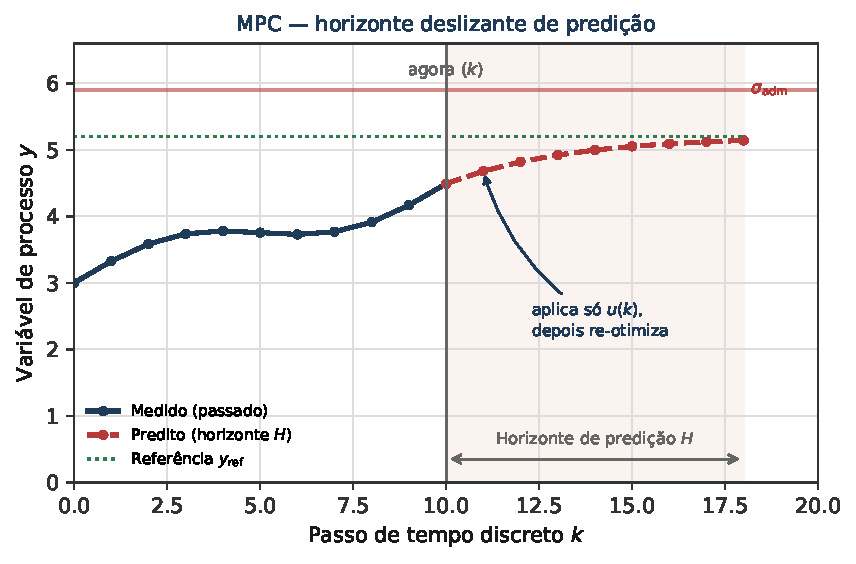
\includegraphics[width=0.60\textwidth]{figuras/fig_24_1_mpc.pdf}
		\caption[Princípio de horizonte deslizante do MPC]{Princípio de horizonte deslizante do MPC: a trajetória prevista (tracejada) é otimizada até o fim do horizonte $H$, mas só a primeira ação de controle é aplicada antes de reotimizar.}
		\label{fig:24-1}
	\end{figure}

	A Equação~\eqref{eq:s24-1} formaliza esse princípio na formulação quadrática padrão do MPC \cite[Cap.~2]{rawlings}: um primeiro somatório penalizando o desvio quadrático da saída em relação à referência ao longo de todo o horizonte, e um segundo penalizando o esforço de controle — ambos sujeitos ao modelo de predição do processo e às restrições de integridade mecânica. A escolha do quadrado não é estética: é ela que torna o problema convexo no caso linear e, portanto, resolúvel de forma confiável dentro do período de amostragem do controlador.

	\begin{equation}\label{eq:s24-1}
	\begin{aligned}
		\text{Minimizar } J &= \sum_{k=1}^{H} [ y(k) - y_{\text{ref}}(k) ]^2 + \rho \sum_{k=0}^{H-1} [ \Delta u(k) ]^2 \\[4pt]
		\text{Sujeito a: } & x_{k+1} = f(x_k, u_k) \\
		& \sigma_b(k) \le \sigma_{\text{adm}}
	\end{aligned}
\end{equation}
	É essa reotimização a cada passo — e não um cálculo único offline — que permite ao MPC reagir a distúrbios reais (uma flutuação de demanda, um desvio de temperatura) sem violar a restrição estrutural $\sigma_b(k) \le \sigma_{\text{adm}}$ em nenhum ponto do horizonte projetado.

	\subsubsection*{Sintonia do horizonte e do peso de esforço}

	Os dois parâmetros livres da Equação~\eqref{eq:s24-1} governam o comportamento do controlador, e ambos têm interpretação física direta neste equipamento.

	O horizonte $H$ deve cobrir a \textbf{dinâmica mais lenta} que o controlador precisa antecipar. Num sistema de ar comprimido, a constante de tempo dominante não é a do compressor, e sim a do vaso pulmão: a Equação~\eqref{eq:s3-5} descreve a dinâmica de pressão desse volume, e é ela que dita quanto tempo o sistema leva para responder a uma mudança de carga. Um horizonte curto demais faz o MPC agir como um PID míope, reagindo à pressão atual sem antecipar o esvaziamento do pulmão; um horizonte longo demais multiplica o custo computacional sem ganho, porque a incerteza da predição cresce e as ações do fim do horizonte são descartadas de qualquer modo. A regra prática é dimensionar $H$ para algo entre uma e duas constantes de tempo do vaso.

	O peso $\rho$ penaliza a \textbf{variação} da ação de controle, $\Delta u$, e não seu valor absoluto — distinção essencial. É ele que impede o controlador de perseguir cada flutuação de pressão com mudanças bruscas de frequência do VSD. Um $\rho$ baixo demais produz ciclagem do inversor: o controlador tecnicamente minimiza o erro, mas ao custo de fadiga térmica no motor e desgaste acelerado, degradando exatamente os componentes cuja vida útil o Gêmeo Digital deveria preservar. Trata-se, portanto, de um parâmetro que acopla o desempenho de controle à integridade mecânica, e sua sintonia deve considerar as duas coisas.

	\subsubsection*{Viabilidade e amolecimento de restrições}

	Há uma falha de projeto que derruba controladores MPC em campo e raramente aparece na formulação teórica: a \textbf{inviabilidade}. Se um distúrbio levar a máquina a um estado a partir do qual nenhuma sequência de ações satisfaz todas as restrições dentro do horizonte, o otimizador não retorna uma solução ruim — ele não retorna solução alguma. O controlador fica sem saída a aplicar, exatamente no momento de maior estresse do sistema.

	A proteção padrão é distinguir restrições \textbf{duras}, que jamais podem ser relaxadas, de restrições \textbf{brandas}, que podem ser violadas temporariamente a um custo alto. Isso se implementa com variáveis de folga $\varsigma \ge 0$ penalizadas na função objetivo, conforme a Equação~\eqref{eq:s24-2}:

	\begin{equation}\label{eq:s24-2}
	\begin{aligned}
		\text{Minimizar } J' &= J + \varrho_s \sum_{k=1}^{H} \varsigma_k^2 \\[4pt]
		\text{Sujeito a: } & \sigma_b(k) \le \sigma_{\text{adm}} && \text{(dura — integridade mecânica)} \\
		& T_{\text{dp}}(k) \le T_{\text{dp,set}} + \varsigma_k && \text{(branda — qualidade do ar)} \\
		& \varsigma_k \ge 0
	\end{aligned}
\end{equation}

	Onde $\varrho_s$ é uma penalidade deliberadamente alta, escolhida de modo que o otimizador só recorra à folga quando não houver alternativa viável. A classificação de cada restrição é uma decisão de engenharia com consequência de segurança, e deve ser explícita: a tensão na raiz do dente é \textbf{dura} porque sua violação é ruptura mecânica, irreversível; o ponto de orvalho é \textbf{brando} porque uma excursão de alguns minutos acima do setpoint durante um transiente de demanda degrada a qualidade do ar temporariamente, sem dano permanente ao equipamento. Confundir as duas categorias — endurecendo tudo — é a receita para um controlador que trava justamente quando é mais necessário.

	\subsubsection*{Modelo de predição e custo computacional}

	A restrição $x_{k+1} = f(x_k, u_k)$ da Equação~\eqref{eq:s24-1} exige avaliar o modelo físico uma vez por passo do horizonte, a cada iteração do otimizador, a cada ciclo de controle — o produto desses três fatores é o que determina a viabilidade em tempo real. Avaliar diretamente o equacionamento completo da Parte I, com suas correlações de troca térmica e psicrometria, é caro demais para essa multiplicação. É precisamente aqui que o modelo substituto treinado por PIML (Capítulo 23) deixa de ser refinamento acadêmico e vira requisito de arquitetura: ele fornece o mesmo $f(\cdot)$ com custo de avaliação ordens de grandeza menor, mantendo consistência física garantida por construção. A alternativa clássica — linearizar o modelo em torno do ponto de operação e resolver um problema quadrático — é mais barata ainda, mas perde validade justamente nos transientes amplos em que o MPC seria mais útil.

	\subsection{Otimização por Enxame de Partículas (PSO)}
	Introduzido por Kennedy e Eberhart em 1995 como metaheurística inspirada no comportamento social de bandos e cardumes \cite{pso}, o PSO é usado aqui para a sintonização de setpoints globais em superfícies de custo não convexas, utilizando a dinâmica de partículas da Equação~\eqref{eq:s24-3}:
	\begin{equation}\label{eq:s24-3}
 v_{i}^{t+1} = w v_{i}^t + c_1 r_1 (p_{\text{best},i} - x_{i}^t) + c_2 r_2 (g_{\text{best}} - x_{i}^t)
\end{equation}
	A Equação~\eqref{eq:s24-3} atualiza apenas a \textbf{velocidade} de cada partícula; o deslocamento propriamente dito vem da Equação~\eqref{eq:s24-4}, que completa a iteração do algoritmo:

	\begin{equation}\label{eq:s24-4}
	x_i^{t+1} = x_i^t + v_i^{t+1}
\end{equation}

	Os termos das duas equações têm leitura direta:
	\begin{itemize}
		\item $p_{\text{best},i}$: Melhor posição já visitada pela partícula $i$ (memória individual).
		\item $g_{\text{best}}$: Melhor posição já encontrada por todo o enxame (memória coletiva).
		\item $w$: Peso de inércia — controla quanto da velocidade anterior é conservado.
		\item $c_1, c_2$: Coeficientes cognitivo e social, que ponderam a atração pela melhor posição própria e pela melhor do grupo.
		\item $r_1, r_2 \sim \mathcal{U}(0,1)$: Números aleatórios sorteados a cada iteração, que introduzem a estocasticidade responsável pela exploração do espaço de busca.
	\end{itemize}

	\subsubsection*{Sintonia dos coeficientes e critério de parada}

	O peso de inércia $w$ governa o compromisso entre exploração e refinamento, e a prática consolidada é não mantê-lo fixo: iniciar alto (tipicamente próximo de $0{,}9$), favorecendo a varredura ampla do espaço de busca, e decair linearmente até um valor baixo (próximo de $0{,}4$) ao longo das iterações, concentrando o enxame em torno da melhor região encontrada. Um $w$ alto demais em regime permanente impede a convergência — as partículas orbitam o ótimo sem se assentar; um $w$ baixo desde o início faz o enxame colapsar prematuramente no primeiro mínimo local que encontrar, anulando a própria razão de se usar uma metaheurística em lugar de um método de gradiente.

	Os coeficientes $c_1$ e $c_2$ são comumente fixados em torno de $2{,}0$ cada. O desbalanço entre eles tem efeito previsível: $c_2 \gg c_1$ acelera a convergência ao custo de perda de diversidade, com o enxame inteiro perseguindo um único ponto e ficando vulnerável a mínimos locais; $c_1 \gg c_2$ produz o oposto, um enxame disperso que explora bem mas converge devagar.

	O critério de parada não deve ser apenas um número máximo de iterações. Duas condições adicionais são mais informativas: \textbf{estagnação} de $g_{\text{best}}$, isto é, ausência de melhoria relativa significativa por um número consecutivo de iterações, e \textbf{colapso de diversidade}, medido pela dispersão das posições das partículas. Este segundo critério merece destaque porque distingue duas situações que o primeiro confunde: um enxame que parou de melhorar \textit{porque convergiu} e um que parou \textit{porque perdeu diversidade cedo demais} e ficou preso. Só o segundo caso justifica reiniciar a busca com nova semeadura.
	A Figura~\ref{fig:24-2} mostra esse comportamento em duas iterações de um enxame sobre uma superfície de custo hipotética: inicialmente as partículas estão espalhadas e suas velocidades (setas) combinam o puxão em direção à melhor posição já visitada por cada uma ($p_{\text{best}}$) com o puxão em direção à melhor posição já vista por todo o enxame ($g_{\text{best}}$); depois de algumas iterações, o enxame converge e se concentra ao redor do mínimo global encontrado.

	\begin{figure}[h!tbp]
		\centering
		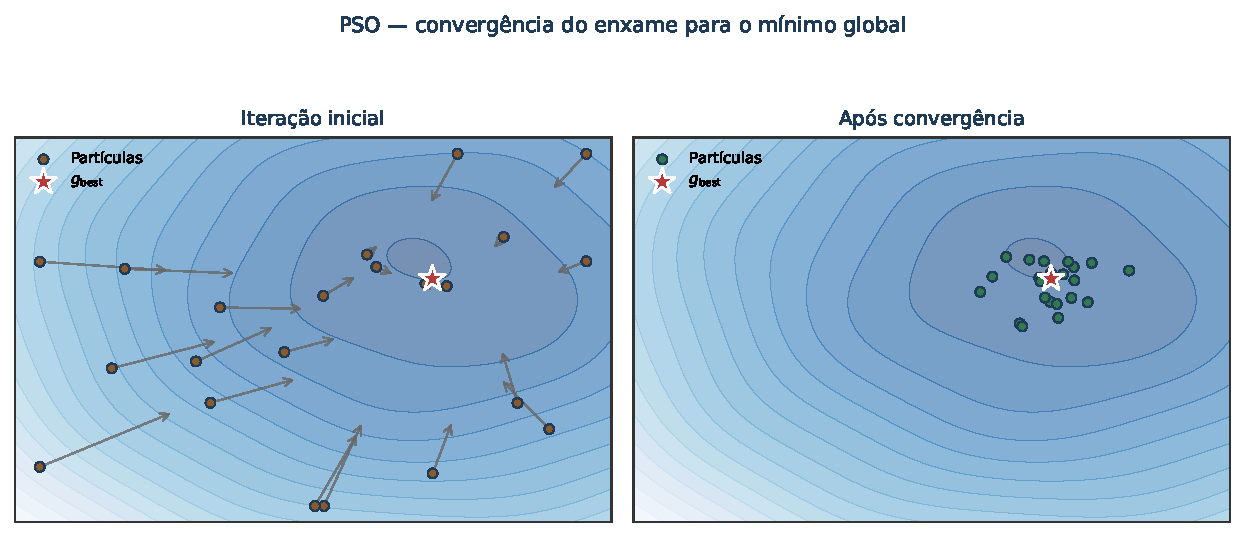
\includegraphics[width=0.75\textwidth]{figuras/fig_24_2_pso.pdf}
		\caption[Convergência do enxame de partículas do PSO]{Convergência do enxame de partículas do PSO sobre uma superfície de custo hipotética: dispersão inicial (esquerda) e concentração em torno do mínimo global $g_{\text{best}}$ após convergência (direita).}
		\label{fig:24-2}
	\end{figure}

	\vspace{1em}
	\hrule
	\vspace{1em}

	\textbf{Diretriz Técnica Final:} MPC e PSO cumprem papéis complementares, não intercambiáveis: o MPC (Equação~\eqref{eq:s24-1}) resolve o controle em tempo real dentro das restrições de integridade, enquanto o PSO é reservado para sintonia de hiperparâmetros e busca de setpoints globais offline — usar PSO no laço de controle em tempo real introduz latência incompatível com a proteção mecânica do compressor. Dois requisitos de projeto decorrem disso e não podem ser omitidos na implementação: o MPC precisa de tratamento explícito de inviabilidade, separando restrições duras de brandas com variáveis de folga (Equação~\eqref{eq:s24-2}), sob pena de o controlador não retornar ação alguma justamente durante o distúrbio que o exigia; e o modelo de predição $f(\cdot)$ deve ser barato o bastante para ser avaliado $H$ vezes por iteração do otimizador, o que na prática torna o substituto treinado por PIML (Capítulo 23) parte da arquitetura de controle, e não um acessório.

	\clearpage
	\section{Diretrizes para o Desenvolvimento e Evolução do Gêmeo Digital}
	
	Este capítulo apresenta recomendações técnicas essenciais para futuros desenvolvedores, focando na robustez, escalabilidade e confiabilidade do sistema em ambientes operacionais offshore.
	
	\subsection{Governança de Dados e Pré-processamento Robusto}
	O sucesso dos algoritmos de inferência, como o EKF e o VAE, depende criticamente da integridade dos sinais de entrada. Em ambientes offshore, a telemetria é frequentemente ruidosa.
	\begin{itemize}
		\item \textbf{Filtragem Adaptativa (Savitzky-Golay):} Diferente de uma média móvel simples — que suaviza o ruído mas também ``arredonda'' picos e mudanças bruscas reais do sinal —, o filtro de Savitzky-Golay \cite{savgol} ajusta um polinômio de grau $p_{\text{SG}}$ por mínimos quadrados dentro de uma janela móvel de $2m_{\text{SG}}+1$ amostras centrada em cada ponto, e usa o valor do polinômio ajustado no centro da janela como a amostra suavizada. Como esse ajuste é linear nos dados de entrada, o resultado se reduz a uma convolução com coeficientes fixos $c_i$ (pré-calculados uma única vez a partir de $p_{\text{SG}}$ e $m_{\text{SG}}$), Equação~\eqref{eq:s25-1}:
		\begin{equation}\label{eq:s25-1}
 y_j^{\text{suav}} = \sum_{i=-m_{\text{SG}}}^{m_{\text{SG}}} c_i \cdotp y_{j+i}
\end{equation}
		É justamente o ajuste polinomial local — em vez de uma média constante — que preserva a amplitude e a largura de transientes reais (como o pico de um impacto mecânico incipiente), ao mesmo tempo em que atenua o ruído de alta frequência da instrumentação; por isso o filtro é preferido à média móvel para os sinais de vibração deste documento.
		\item \textbf{Tratamento de Outliers (\textit{Isolation Forest}):} Ao contrário de métodos que primeiro modelam o que é ``normal'' para depois sinalizar desvios, o \textit{Isolation Forest} \cite{isoforest} explora diretamente a definição de anomalia — pontos raros e diferentes são mais fáceis de isolar. O algoritmo constrói um conjunto de árvores binárias aleatórias (\textit{isolation trees}), cada uma particionando os dados recursivamente por um atributo e um valor de corte escolhidos ao acaso; um ponto anômalo tende a ser isolado em poucas divisões (caminho curto até a raiz da árvore), enquanto um ponto normal exige muitas divisões (caminho longo). O escore de anomalia normaliza o comprimento médio do caminho de isolamento $E[L_{\text{iso}}(x)]$ sobre todas as árvores da floresta pelo comprimento médio esperado numa árvore de busca binária com $n_{\text{IF}}$ pontos, Equação~\eqref{eq:s25-2}:
		\begin{equation}\label{eq:s25-2}
 s_{\text{IF}}(x) = 2^{-\frac{E[L_{\text{iso}}(x)]}{c(n_{\text{IF}})}}, \quad c(n_{\text{IF}}) = 2\left[\ln(n_{\text{IF}}-1) + \gamma_{\text{EM}}\right] - \frac{2(n_{\text{IF}}-1)}{n_{\text{IF}}}
\end{equation}
		Onde $\gamma_{\text{EM}} \approx 0{,}5772$ é a constante de Euler-Mascheroni (subscrita para não colidir com a razão de calores específicos $\gamma$ usada nos capítulos de termodinâmica). Um escore $s_{\text{IF}}$ próximo de 1 indica forte probabilidade de anomalia (caminho de isolamento muito curto); próximo de 0,5, o ponto é indistinguível do comportamento normal. O Gêmeo Digital usa esse escore para filtrar picos espúrios de sensor antes que alimentem o EKF ou o VAE, evitando falsos diagnósticos de falha originados por ruído de instrumentação, não por degradação real do equipamento. A Figura~\ref{fig:25-1} ilustra a ideia geometricamente: um ponto anômalo isolado do resto dos dados é separado do restante em poucos cortes retangulares aleatórios, enquanto um ponto no meio do aglomerado normal só se isola depois de muitos cortes sucessivos.

		\begin{figure}[h!tbp]
			\centering
			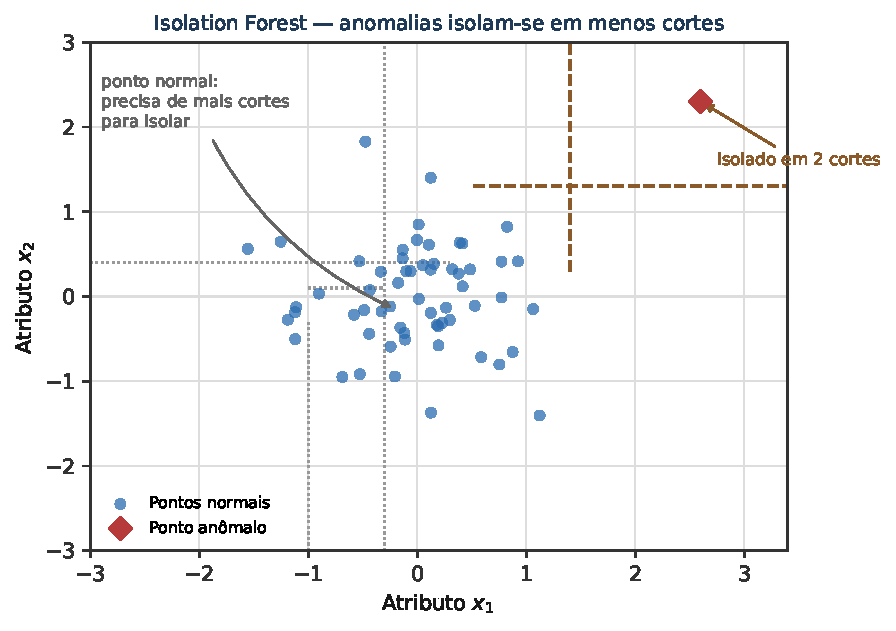
\includegraphics[width=0.60\textwidth]{figuras/fig_25_1_isoforest.pdf}
			\caption[Princípio do \textit{Isolation Forest}]{Princípio do \textit{Isolation Forest}: um ponto anômalo se isola do restante dos dados em poucos cortes aleatórios; um ponto no meio de um aglomerado normal exige muito mais cortes.}
			\label{fig:25-1}
		\end{figure}
	\end{itemize}
	
	\subsection{Quantificação de Incerteza (UQ)}
	Um Gêmeo Digital de missão crítica não deve fornecer apenas valores determinísticos, mas sim intervalos de confiança para suportar a tomada de decisão segura.
	\begin{itemize}
		\item \textbf{Propagação de Erro:} A incerteza dos sensores deve ser propagada para os KPIs globais, como a destruição de exergia ($\dot{I}$). A Equação~\eqref{eq:s25-3} é a fórmula clássica de propagação de incerteza: cada temperatura medida $T_i$ contribui para a incerteza total de $\dot{I}$ na proporção de quão sensível $\dot{I}$ é àquela temperatura específica (a derivada parcial) multiplicada pela incerteza do próprio sensor $u(T_i)$, somadas em quadratura:
		\begin{equation}\label{eq:s25-3}
 u(\dot{I}) = \sqrt{\sum_{i=1}^{n} \left( \frac{\partial \dot{I}}{\partial T_i} \right)^2 u(T_i)^2}
\end{equation}
		\item \textbf{Redes Bayesianas:} Substituição de camadas densas por camadas bayesianas no PIML para obter a variância da predição ($\sigma^2$).
	\end{itemize}
	
	\subsection{Arquitetura de Computação em Borda (Edge Computing)}
	Dada a latência de comunicação via satélite em plataformas, a arquitetura deve ser distribuída para garantir respostas em tempo real.
	\begin{itemize}
		\item \textbf{Processamento Local (Edge):} Algoritmos de alta frequência, como a análise de harmônicos de vibração e o EKF, devem ser executados próximos ao ativo físico.
		\item \textbf{Processamento em Nuvem (Cloud):} O treinamento de modelos pesados (VAE) e a otimização de longo prazo (MPC) devem ser centralizados para aproveitar maior capacidade computacional.
	\end{itemize}
	
	\subsection{Explicabilidade e Interface Humano-Máquina (XAI)}
	Para que o Gêmeo Digital seja aceito pelos operadores, suas decisões devem ser auditáveis e compreensíveis.
	\begin{itemize}
		\item \textbf{Valores de SHAP:} Utilização de \textit{SHapley Additive exPlanations} para quantificar a contribuição de cada sensor em um diagnóstico de falha. A Equação~\eqref{eq:s25-4}, originada da teoria de jogos cooperativos, calcula a contribuição média da variável $x_i$ ($\phi_i$) testando o modelo $f$ com e sem essa variável, em todas as combinações possíveis ($S$) das demais variáveis — o resultado é um ``crédito'' justo de quanto cada sensor pesou na decisão do modelo, permitindo ao operador ver, por exemplo, que um alarme foi disparado principalmente por $T_{dp}$ e não por vibração:
		\begin{equation}\label{eq:s25-4}
 \phi_i(f) = \sum_{S \subseteq \{x_1, \dots, x_n\} \setminus \{x_i\}} \frac{|S|! (n - |S| - 1)!}{n!} [f(S \cup \{x_i\}) - f(S)]
\end{equation}
		\item \textbf{Visualização Latente:} Projeção do espaço latente do VAE em duas dimensões para visualização intuitiva da trajetória de degradação do ativo.
	\end{itemize}
	
	\subsection{Ciclo de Vida e MLOps (Model Drift)}
	O ativo físico sofre modificações estruturais ao longo do tempo (substituição de componentes, novos selos). O modelo digital deve evoluir em sincronia com o físico.
	\begin{itemize}
		\item \textbf{Detecção de Drift:} Monitoramento contínuo do erro de reconstrução do VAE. Se o erro crescer consistentemente após uma manutenção, o modelo deve ser retreinado.
		\item \textbf{Pipeline de Retreinamento:} Automação do fluxo de coleta de dados históricos para ajuste dos pesos sinápticos ($\theta, \phi$) do modelo híbrido.
	\end{itemize}
	
	\vspace{1em}
	\hrule
	\vspace{1em}
	
	\textbf{Diretriz Técnica Final:} O desenvolvedor deve tratar o Gêmeo Digital como um organismo vivo. A calibração contínua via EKF e a consistência física via PIML são os diferenciais que garantem a segurança estrutural e a eficiência exergética em tempo real.
	
	\newpage

	\clearpage
	\section{Implementação Base e Ferramentas Padrão}

	Este capítulo descreve a infraestrutura fundamental e a lógica de programação para a execução do Gêmeo Digital em ambiente de produção, utilizando bibliotecas de código aberto consagradas e integração com sistemas legados.
	
	\subsection{Stack Tecnológica de Referência}
	Para garantir a interoperabilidade entre os modelos físicos e de aprendizado de máquina, recomenda-se a seguinte configuração:
	\begin{itemize}
		\item \textbf{Linguagem Principal:} Python $3.9+$.
		\item \textbf{Ingestão de Dados:} \text{OSIsoft PI Web API} ou \text{MQTT} para comunicação em tempo real.
		\item \textbf{Processamento Numérico:} \text{NumPy} e \text{SciPy} para álgebra linear e integração.
		\item \textbf{Deep Learning (VAE e PIML):} \text{PyTorch} ou \text{TensorFlow}.
		\item \textbf{Otimização e MPC:} \text{CasADi} ou \text{Pyomo} para resolução de problemas de controle ótimo não linear (NLP).
		\item \textbf{Banco de Dados:} \text{InfluxDB} ou \text{TimescaleDB} para armazenamento de séries temporais.
	\end{itemize}
	
	\subsection{Implementação do Filtro de Kalman Estendido (EKF)}
	O EKF é o motor de fusão de dados que estima variáveis ocultas (como a folga residual $\delta$) a partir de medições ruidosas, no ciclo de predição-correção da Equação~\eqref{eq:s26-1}:
	\begin{equation}\label{eq:s26-1}
	\begin{aligned}
		\text{Predição:} \quad \hat{x}_{k|k-1} &= f(\hat{x}_{k-1|k-1}, u_{k-1}) \\[4pt]
		P_{k|k-1} &= F_k P_{k-1|k-1} F_k^T + Q \\[8pt]
		\text{Correção:} \quad K_k &= P_{k|k-1} G_k^T (G_k P_{k|k-1} G_k^T + \mathcal{R})^{-1} \\[4pt]
		\hat{x}_{k|k} &= \hat{x}_{k|k-1} + K_k (z_k - g(\hat{x}_{k|k-1}))
	\end{aligned}
\end{equation}
	
	A implementação abaixo segue as recomendações de robustez numérica do Capítulo 21: a covariância é atualizada pela forma de Joseph (Equação~\eqref{eq:s21-8}) em vez da forma simplificada, e a inovação e o NIS (Equação~\eqref{eq:s21-7}) são devolvidos junto com o estado, para que a camada superior possa auditar a consistência do filtro em tempo real.

	\begin{verbatim}
import numpy as np

def ekf_update(x_hat, P, z, u, Q, R_meas, dt):
    # 1. Predição (modelo físico politrópico)
    x_pred = f_physics(x_hat, u, dt)
    F = compute_jacobian_f(x_hat, u, dt)
    P_pred = F @ P @ F.T + Q

    # 2. Correção (medição de P, T e vazão)
    G = compute_jacobian_g(x_pred)
    y_res = z - g_observation(x_pred)      # inovação
    S = G @ P_pred @ G.T + R_meas          # covariância da inovação
    K = P_pred @ np.linalg.solve(S, G).T   # evita inv(S) explícita

    x_new = x_pred + K @ y_res

    # 3. Covariância pela forma de Joseph (estável)
    I_KG = np.eye(len(x_hat)) - K @ G
    P_new = I_KG @ P_pred @ I_KG.T + K @ R_meas @ K.T
    P_new = 0.5 * (P_new + P_new.T)        # força simetria

    # 4. Auditoria: NIS ~ chi2(n_z) se o filtro estiver consistente
    nis = float(y_res.T @ np.linalg.solve(S, y_res))
    return x_new, P_new, y_res, nis
\end{verbatim}

	Três detalhes desse trecho merecem comentário, porque são justamente os que costumam ser omitidos em implementações de protótipo e cobrados em produção. O uso de \texttt{np.linalg.solve} em lugar de \texttt{np.linalg.inv} resolve o sistema linear sem formar a inversa explicitamente — numericamente mais estável e mais barato, e a diferença se acumula ao longo de milhões de ciclos. A simetrização forçada de \texttt{P\_new} corrige a assimetria residual introduzida por arredondamento, que de outro modo se amplifica a cada iteração. E o retorno do NIS é o que transforma o filtro de caixa-preta em instrumento auditável: sem ele, não há como distinguir em campo um EKF saudável de um que já divergiu silenciosamente.
	
	\subsection{Função de Perda Physics-Informed (PIML)}
	A rede neural é treinada, pela Equação~\eqref{eq:s26-2}, para minimizar o erro dos dados enquanto satisfaz o balanço de energia:
	\begin{equation}\label{eq:s26-2}
 L_{\text{total}} = \text{MSE}_{\text{data}} + \lambda \cdotp \text{MSE}_{\text{phys}} 
\end{equation}
	\begin{verbatim}
import torch

def piml_loss(y_pred, y_true, inputs, lambda_phys):
    data_loss = torch.mean((y_pred - y_true)**2)

    # Resíduo físico: W_dot - m_dot * cp * (T_out - T_in) = 0
    m_dot = inputs[:, 0]
    cp = 1005.0                            # J * kg^-1 * K^-1
    W_dot = compute_power(inputs)
    phys_residual = W_dot - m_dot * cp * (y_pred[:, 3] - y_pred[:, 1])
    phys_loss = torch.mean(phys_residual**2)

    return data_loss + lambda_phys * phys_loss
\end{verbatim}
	
	\subsection{Indicadores Globais de Saúde (KPIs)}
	\begin{itemize}
		\item \textbf{Eficiência Exergética:} Razão entre a exergia efetivamente aproveitada e a exergia total de entrada, conforme a Equação~\eqref{eq:s26-3}:
		\begin{equation}\label{eq:s26-3}
 \eta_{\text{ex}} = 1 - \frac{\dot{I}}{\dot{E}x_{\text{in}}}
\end{equation}
		\item \textbf{Health Index (HI):} Normalização ponderada dos resíduos do VAE e do EKF, definida a seguir.
	\end{itemize}

	O \textit{Health Index} merece definição explícita, por ser o número que efetivamente chega ao operador. Ele condensa indicadores de naturezas distintas — um resíduo estatístico de reconstrução, um estado físico estimado, um desvio de eficiência — numa escala única de $0$ a $1$, onde $1$ representa a máquina em condição de referência. A dificuldade é que esses indicadores têm unidades e faixas incomparáveis, o que exige normalizar cada um pelo seu próprio limiar antes de combinar, conforme a Equação~\eqref{eq:s26-4}:

	\begin{equation}\label{eq:s26-4}
	HI = 1 - \sum_{j} \varpi_j \cdot \min\left( 1,\; \frac{\max(0,\; \Theta_j - \Theta_{j,\text{ref}})}{\Theta_{j,\text{lim}} - \Theta_{j,\text{ref}}} \right), \qquad \sum_j \varpi_j = 1
\end{equation}

	Onde $\Theta_j$ é o $j$-ésimo indicador (erro de reconstrução do VAE, folga estimada pelo EKF, queda de eficiência isentrópica, destruição exergética), $\Theta_{j,\text{ref}}$ seu valor na condição de referência, $\Theta_{j,\text{lim}}$ o valor em que aquele indicador isoladamente caracteriza falha, e $\varpi_j$ o peso atribuído. Os símbolos $\Theta$ e $\varpi$ foram escolhidos por serem os únicos livres nesta faixa do alfabeto grego: $\zeta$ já designa o coeficiente de perda dos filtros e $\omega$ a velocidade angular. As duas saturações não são detalhe cosmético: o $\max(0,\cdot)$ impede que um indicador melhor que a referência compense artificialmente outro degradado — uma máquina com trocador limpo não fica ``saudável'' por isso apesar de um mancal em fim de vida — e o $\min(1,\cdot)$ impede que um único indicador em colapso arraste o índice para valores negativos sem significado.

	Cabe um alerta sobre o uso desse número. O HI é uma ferramenta de \textbf{comunicação e priorização}, útil para ordenar máquinas de uma frota por urgência de intervenção. Ele não é, e não deve ser tratado como, base para decisão de proteção: a agregação ponderada é intrinsecamente uma perda de informação, e um HI de $0{,}8$ não distingue quatro indicadores levemente degradados de um único indicador em situação crítica. As decisões de trip e alarme pertencem à matriz da Tabela~\ref{tab:18-2}, que opera sobre os indicadores individuais.

	\subsection{Requisitos de Passagem para Produção}

	A distância entre o código acima e um Gêmeo Digital em operação contínua é maior do que a extensão dos trechos sugere, e essa distância é composta por itens de engenharia, não de modelagem.

	\begin{itemize}
		\item \textbf{Versionamento conjunto de modelo e dados:} um modelo treinado é a composição de pesos, hiperparâmetros e do conjunto exato que o originou. Reproduzir um diagnóstico emitido meses antes — exigência corriqueira numa investigação de falha — requer os três, versionados juntos.
		\item \textbf{Testes de regressão contra falhas conhecidas:} todo evento de falha documentado na planta deve virar um caso de teste, com o critério de que o modelo o detecte com a antecedência registrada. Uma versão nova que melhora a métrica agregada mas deixa de detectar uma falha antes capturada é uma regressão, ainda que os números globais tenham melhorado.
		\item \textbf{Monitoramento de deriva (\textit{model drift}):} a distribuição dos dados de entrada muda com trocas de peça, mudanças de regime operacional e envelhecimento. Deve haver detecção automática dessa deriva, disparando reavaliação — não retreinamento cego, que reintroduziria o problema de contaminação do conjunto de treino discutido no Capítulo 22.
		\item \textbf{Degradação graciosa:} a perda de um sensor não pode derrubar o Gêmeo Digital. O sistema precisa reconhecer a indisponibilidade, reavaliar a observabilidade dos estados afetados (Equação~\eqref{eq:s21-5}) e sinalizar explicitamente quais estimativas deixaram de ter suporte, em vez de continuar publicando números.
		\item \textbf{Rastreabilidade da decisão:} toda ação automática executada deve registrar as entradas, o estado estimado e a versão de modelo que a produziram. Sem isso não há auditoria de incidente possível — e, num ambiente offshore sujeito a requisitos de segurança de processo, não há como demonstrar a lógica que levou o sistema a agir.
	\end{itemize}

	\subsection{Painel Supervisório de Frota}

	Todo o capítulo até aqui — e o simulador de referência que o acompanha — trata o Gêmeo Digital como um cálculo executado para \textbf{uma} máquina, disparado sob demanda para \textbf{um} cenário: um ponto de operação é montado, os algoritmos rodam uma vez, um diagnóstico sai. Uma instalação offshore real opera $N_{\text{frota}}$ máquinas simultaneamente (Equação~\eqref{eq:s16-1}), continuamente, não sob demanda — e é essa lacuna, entre o protótipo de análise pontual e o \textbf{painel supervisório}, que os cinco requisitos de produção da subseção anterior preparam mas não fecham sozinhos.

	O painel supervisório não introduz algoritmo novo: ele repete, para cada máquina $i \in \{1, \dots, N_{\text{frota}}\}$ e a cada ciclo de varredura $t_k$, exatamente o ciclo já definido neste documento — predição-correção do EKF (Equação~\eqref{eq:s26-1}), atualização do Health Index (Equação~\eqref{eq:s26-4}) e verificação da matriz de alarmes (Tabela~\ref{tab:18-2}) — e acumula o resultado como uma \textbf{série temporal por máquina}, não um número isolado, publicado uma vez e descartado. O trecho abaixo formaliza esse laço, reaproveitando a mesma função \texttt{ekf\_update} já definida nesta seção:

	\begin{verbatim}
def ciclo_supervisorio(frota, t_k):
    painel = []
    for maquina in frota:
        x_new, P_new, y_res, nis = ekf_update(
            maquina.x_hat, maquina.P, maquina.z(t_k),
            maquina.u(t_k), maquina.Q, maquina.R_meas,
            dt=t_k - maquina.t_last)
        maquina.x_hat, maquina.P, maquina.t_last = x_new, P_new, t_k

        hi = health_index(maquina.residuos(x_new))    # Eq. 26.4
        alarmes = verificar_alarmes(maquina.z(t_k))    # Tabela 18.2

        painel.append({"maquina": maquina.id, "t": t_k,
                        "hi": hi, "nis": nis, "alarmes": alarmes})

    # urgencia: alarme ativo primeiro, depois menor HI
    painel.sort(key=lambda m: (not m["alarmes"], m["hi"]))
    return painel
	\end{verbatim}

	Duas decisões desse laço merecem destaque, porque são exatamente onde um painel construído sem cuidado costuma falhar. Primeiro, a \textbf{ordenação por urgência}, não por identificador de máquina: a subseção de Indicadores Globais de Saúde já advertiu que o $HI$ é ferramenta de priorização, não de proteção — o painel aplica esse conselho diretamente, listando primeiro qualquer máquina com alarme ativo (independente do $HI$) e, entre as demais, a de menor $HI$. Segundo, o NIS de cada máquina (Equação~\eqref{eq:s21-7}) é propagado junto com o $HI$, não descartado: um $HI$ baixo sustentado por um filtro já divergente é uma leitura sem valor, e o operador precisa distinguir ``máquina degradando'' de ``estimativa não confiável'' — a mesma distinção que o Capítulo 21 já exige numa única máquina, aqui elevada ao nível do painel inteiro.

	O prognóstico de vida remanescente de cada máquina acompanha o mesmo princípio: a regressão por Processo Gaussiano da Equação~\eqref{eq:s19-10} — a mesma usada pontualmente no Capítulo 29 para $RUL_\delta$ — se recalcula por máquina a cada ciclo, a partir da série acumulada de $\hat\delta_i(t)$ do EKF daquela unidade com intervalo de confiança de $95\%$, em vez de ser recalculada do zero apenas quando um operador decide investigar.

	\subsection{Topologia Dinâmica de Trens e Filosofias de Redundância}
	Em instalações offshore, os compressores são agrupados em trens em paralelo compartilhando a sucção e a descarga no vaso pulmão. O Gêmeo Digital suporta topologias escaláveis de $N_{\text{frota}} \in [1, 12]$ máquinas com capacidades unitárias ($\text{FAD}_i \in [5, 80]\text{ m}^3/\text{min}$), avaliando três filosofias de redundância operacional:
	\begin{enumerate}
		\item \textbf{Redundância $N+0$ (Sem Reserva):} Todas as máquinas operam próximas da capacidade nominal ($\Sigma \dot{m}_{\text{comp}} \approx \dot{m}_{\text{dem}}$). Apresenta menor custo de capital inicial, porém vulnerabilidade total a paradas não programadas.
		\item \textbf{Redundância $N+1$ (Padrão Offshore / FPSO):} Uma unidade opera em \textit{standby} quente ou alívio com modulação VSD, assumindo a carga instantaneamente em caso de trip ou manutenção preventiva de qualquer uma das $N$ unidades ativas.
		\item \textbf{Redundância $2N$ (Dupla Redundância Integral):} Dois trens independentes de $100\%$ de capacidade, reservada para serviços críticos de segurança de processo e instrumentação de emergência (ESD).
	\end{enumerate}

	\vspace{1em}
	\hrule
	\vspace{1em}

	\textbf{Diretriz Técnica Final:} A implementação de referência deste capítulo (EKF em NumPy puro, PIML em PyTorch) é suficiente para prototipagem e validação offline; migrar para produção contínua exige a formalização de trens flexíveis, supervisão agregada por prioridade de alarme e integração nativa com barramentos industriais de alta velocidade (OSIsoft PI System).

	\newpage
	
	\clearpage
	\section{Implementação de Alta Performance e Physics-ML}
	
	Este capítulo detalha o uso de frameworks de vanguarda para simulações de alta fidelidade, operadores neurais e a transição para arquiteturas de software nativas compiladas em tempo real.
	
	\subsection{Frameworks de Physics-ML (NVIDIA Modulus)}
	O uso do \textbf{NVIDIA Modulus} \cite{modulus} permite a criação de \text{Surrogate Models} baseados em PINNs e Operadores Neurais de Fourier (FNO) que substituem solvers de CFD lentos.
	\begin{itemize}
		\item \textbf{Vantagem:} Redução do tempo de simulação de horas para milissegundos.
		\item \textbf{Funcionalidade:} Integração direta de geometrias CAD e equações de Navier-Stokes.
	\end{itemize}
	
	\subsection{Solvers de PDEs e Problemas Inversos (DeepXDE)}
	O \textbf{DeepXDE} \cite{deepxde} é utilizado para estimar parâmetros de degradação (como rugosidade interna) minimizando o resíduo das equações diferenciais da Equação~\eqref{eq:s27-1}:
	\begin{equation}\label{eq:s27-1}
 \mathcal{R}(\mathbf{u}) = \rho (\mathbf{u} \cdotp \nabla) \mathbf{u} + \nabla p - \mu \nabla^2 \mathbf{u} = 0 
\end{equation}
	
	\subsection{Controle Preditivo e MHE (do-mpc)}
	O pacote \textbf{do-mpc} \cite{dompc} oferece suporte para \text{Moving Horizon Estimation} (MHE), superior ao EKF em lidar com restrições severas e incertezas de modelo, integrando-se nativamente ao CasADi.
	
	\subsection{Arquitetura Nativa de Produção em Rust (Axum / Tokio)}
	Embora ambientes interpretados baseados em Python sejam ideais para prototipagem rápida e validação de equações, a operação de Gêmeos Digitais industriais de missão crítica (com múltiplos trens de compressores e telemetria OSIsoft PI em alta frequência) impõe requisitos severos de latência determinística e consumo de memória.
	
	A reescrita industrial em linguagem \textbf{Rust} (compilada nativamente com otimizações LLVM e servidor assíncrono Axum/Tokio) demonstrou ganhos substanciais de desempenho mantendo exata fidelidade analítica ($\Delta < 10^{-7}$):
	\begin{itemize}
		\item \textbf{Throughput de Simulação Estática:} Aceleração de $7.6\times$ ($13.17\ \mu\text{s}$ por simulação de 7 nós em Rust versus $100.75\ \mu\text{s}$ em Python), atingindo mais de $75.000$ simulações completas por segundo.
		\item \textbf{Dinâmica Transiente de Vasos (ASME VIII):} Aceleração de $30.7\times$ ($0.22\text{ ms}$ em Rust contra $6.72\text{ ms}$ em Python para integração de $3.600$ passos de Euler), permitindo previsões antecipatórias em tempo real no laço do MPC.
		\item \textbf{Otimização Global PSO:} Aceleração de $63.1\times$ ($0.016\text{ ms}$ por convergência em Rust versus $1.01\text{ ms}$ em Python).
		\item \textbf{Consumo de Memória RAM:} Redução de $\approx 25\times$ na pegada de memória ($~10\text{ MB}$ em binário estático Rust contra $~280\text{ MB}$ em ambiente Python/PyTorch), viabilizando implantação em servidores de borda (\textit{Edge Computing} no FPSO) sem concorrência de recursos com o SCADA.
	\end{itemize}
	
	\subsection{Resumo da Stack de Vanguarda}
	A Tabela~\ref{tab:27-1} consolida a divisão de responsabilidades entre as camadas do Gêmeo Digital, comparando a stack analítica de pesquisa com a stack de produção nativa.

	\begin{table}[h!tbp]
	\centering
	\resizebox{\textwidth}{!}{%
	\begin{tabular}{llll}
		\toprule
		\textbf{Camada} & \textbf{Ferramenta (Pesquisa)} & \textbf{Ferramenta (Produção)} & \textbf{Função} \\ \midrule
		Motor Termodinâmico & Python / NumPy & Rust (\texttt{sim\_core}) & Balanço de 7 nós e transiente ASME VIII \\
		Filtro de Estados / EKF & SciPy & Rust (\texttt{ndarray}) & Fusão sensorial e teste NIS $\chi^2$ \\
		Controle / Otimização & CasADi / do-mpc & Rust (\texttt{mpc}/\texttt{pso}) & Otimização de setpoint $\pi^*$ e VSD \\
		Servidor & Streamlit & Axum / Tokio & API REST assíncrona ($<0.5\text{ ms}$) \\
		Telemetria & PI Web API & OSIsoft PI / Modbus & Mapeamento de 26+ tags ISA 18.2 \\ \bottomrule
	\end{tabular}%
	}
	\caption[Camadas da stack de alta performance]{Divisão de responsabilidades entre as camadas do Gêmeo Digital: pesquisa versus produção de alta performance.}
	\label{tab:27-1}
	\end{table}

	\vspace{1em}
	\hrule
	\vspace{1em}

	\textbf{Diretriz Técnica Final:} A transição para frameworks como o \textbf{Modulus} e \textbf{do-mpc} permite que o Gêmeo Digital realize simulações ``What-If'' complexas com precisão física e velocidade de resposta instantânea.

\clearpage
\thispagestyle{empty}
\phantomsection
\addcontentsline{toc}{part}{Parte III --- Estudo de Caso Integrado}
\vspace*{\fill}
\begin{center}
	{\Huge\bfseries PARTE III}\\[2em]
	{\huge\bfseries Estudo de Caso Integrado}
\end{center}
\vspace*{\fill}
\clearpage

% --- Início do Capítulo 28: Metodologia de Calibração de Parâmetros e Catálogo de Detecção ---

\clearpage
\section{Metodologia de Calibração de Parâmetros e Catálogo de Detecção}
\markboth{Metodologia de Calibração e Catálogo de Detecção}{}

Os Capítulos 21 a 27 descreveram como o Gêmeo Digital estima \textbf{estados} que variam com o tempo — folga, incrustação, eficiência isentrópica — a partir de um modelo físico que, até aqui, tratou seus próprios parâmetros como constantes conhecidas. Na prática de campo isso raramente é verdade: a Equação~\eqref{eq:s9-3} já qualifica o coeficiente de vazamento $K$ como algo ``calibrado por ensaio de desempenho da máquina'', mas nenhum capítulo anterior descreveu como fazer esse ensaio de forma sistemática, nem o que fazer quando ele não é possível. Este capítulo fecha essa lacuna metodológica em quatro passos, na ordem em que um comissionamento real os enfrentaria: primeiro, como calibrar os parâmetros estáticos do modelo a partir de dados de uma janela de operação sabidamente saudável (Seção~28.1); segundo, como registrar de forma explícita e auditável o que continua desconhecido depois dessa calibração, em vez de deixar essa lacuna implícita (Seção~28.2); terceiro, um catálogo consolidado ligando cada mecanismo de falha já descrito na Parte I ao algoritmo da Parte II mais adequado para detectá-lo (Seção~28.3); e quarto, a verificação quantitativa de que essa indicação de algoritmo é sustentada pelo próprio modelo direto, para o subconjunto do catálogo em que isso é hoje simulável (Seção~28.4). O Capítulo 29 aplica as quatro peças em conjunto, num cenário numérico único.

\subsection{Estimação Conjunta de Estado e Parâmetro (EKF com Estado Aumentado)}

Além de $K$, outros parâmetros do modelo físico da Parte I nunca foram medidos nesta máquina específica: $\eta_{\text{mec}}$ (eficiência mecânica do elemento compressor, Equação~\eqref{eq:s5-5}), o coeficiente de perda de filtro em condição limpa, $\zeta_{\text{ref}}$ (Equações~\eqref{eq:s3-4}/\eqref{eq:s5-4}), e, para as válvulas de alívio e retenção, o coeficiente de perda de referência $\zeta_{\text{valv,ref}}$ (Equação~\eqref{eq:s5-16}) — entram no equacionamento como valores de catálogo ou de literatura — calibrados pelo fabricante em condições padronizadas de bancada, não na instalação real. Essa premissa raramente se sustenta: o próprio $K$ já é descrito, na Equação~\eqref{eq:s9-3}, como calibrado por ensaio de desempenho \textit{da máquina}, precisamente porque agrega efeitos de geometria e usinagem que variam de um lote de rotores para outro; $\eta_{\text{mec}}$ muda com o alinhamento e a lubrificação de campo; $\zeta_{\text{ref}}$ depende do elemento filtrante efetivamente especificado em cada obra, que varia entre plataformas e fornecedores. Determinar esses parâmetros a partir de medições indiretas, em vez de assumi-los fixos, é um \textbf{problema inverso}: no problema direto, conhecidos os parâmetros, calcula-se a resposta do sistema; aqui se observa a resposta (as medições de campo desta instalação específica) e busca-se o parâmetro causal que a produziu — a mesma dualidade que fundamenta a formulação de PINNs do Capítulo 23 \cite{piml}, aplicada aqui por um mecanismo diferente. Esta seção resolve esse problema inverso com a técnica padrão de \textbf{estimação conjunta de estado e parâmetro} (\textit{joint/dual state-parameter estimation}) \cite{simon}: em vez de tratar esses parâmetros como constantes externas ao filtro, eles passam a integrar o próprio vetor de estado do EKF, na Equação~\eqref{eq:s28-1}:

\begin{equation}\label{eq:s28-1}
x_{\text{aug}} = \begin{bmatrix} x \\ \Lambda \end{bmatrix}, \qquad \Lambda = \begin{bmatrix} K \\ \eta_{\text{mec}} \\ \zeta_{\text{ref}} \\ \zeta_{\text{valv}} \end{bmatrix}
\end{equation}

Onde $x$ é o mesmo vetor de estado dinâmico da Equação~\eqref{eq:s21-2} — as variáveis de degradação, que continuam a variar com o tempo — e $\Lambda$ é o vetor dos parâmetros estáticos escolhidos como exemplo para este trem de compressão; a lista não é exaustiva, e qualquer outro parâmetro de catálogo do modelo físico pode ser aumentado da mesma forma, seguindo o protocolo da Seção~28.2 para decidir quais valem a pena. O modelo de transição do estado aumentado, Equação~\eqref{eq:s28-2}, propaga $x$ pela mesma dinâmica não linear $f$ da Equação~\eqref{eq:s21-1} — agora explicitamente parametrizada por $\Lambda$ — e trata os parâmetros estáticos como um passeio aleatório de covariância controlável:

\begin{equation}\label{eq:s28-2}
\begin{bmatrix} x_k \\ \Lambda_k \end{bmatrix} = \begin{bmatrix} f(x_{k-1}, \Lambda_{k-1}, u_{k-1}) \\ \Lambda_{k-1} \end{bmatrix} + w_{\text{aug},k-1}, \qquad Q_{\text{aug}} = \begin{bmatrix} Q & 0 \\ 0 & Q_\Lambda \end{bmatrix}
\end{equation}

O ganho da técnica está inteiramente em como $Q_\Lambda$ é escolhido ao longo do tempo, não numa equação nova: o ciclo de predição-correção em si continua sendo exatamente o da Equação~\eqref{eq:s21-4}, aplicado ao vetor aumentado $x_{\text{aug}}$ no lugar de $x$. Durante uma \textbf{janela de calibração} — comissionamento, ou o período imediatamente após uma manutenção confirmada, quando se sabe por outros meios (inspeção, relatório de serviço) que a máquina está numa condição de referência conhecida — $Q_\Lambda$ é fixado próximo de zero: o filtro trata $\Lambda$ como verdadeiramente constante, o que acelera a convergência e produz a melhor estimativa possível dos parâmetros com os dados daquela janela. Terminada a calibração, $Q_\Lambda$ passa a um valor pequeno mas não nulo, permitindo que o filtro acompanhe deriva lenta genuína — o próprio $K$ tende a crescer ao longo de anos por desgaste do perfil do rotor — sem descartar de uma vez a informação acumulada na janela de calibração.

Essa mecânica de convergência — uma crença inicial pouco informativa que se estreita ao longo de vários ciclos até um valor sustentado pelos dados — já tem precedente de implementação prática na ferramenta de referência que acompanha este documento, em duas camadas. O módulo EKF do simulador (\texttt{aplicativo/compressor\_sim/ekf.py}, função \texttt{simular\_ekf()}) implementa o ciclo de predição-correção da Equação~\eqref{eq:s21-4} para os dois estados dinâmicos com contraparte calculável no simulador (folga relativa e incrustação equivalente do intercooler), sem nenhum parâmetro estático aumentado. A função \texttt{simular\_ekf\_aumentado()} do mesmo módulo vai além: implementa de fato o estado aumentado das Equações~\eqref{eq:s28-1}/\eqref{eq:s28-2} — $x_{\text{aug}} = [\text{folga\_rel}, r_{f,\text{equiv}}, K]$ — com dois regimes de $Q_\Lambda$ para $K$, mas na ordem \textbf{inversa} da descrita acima: durante a janela de calibração, $Q_K$ é normal/ativo (o filtro deixa $K$ convergir livremente a partir de um prior pouco informativo — exploração ativa, não um valor quase constante); terminada a calibração, $Q_K$ cai a quase zero, ``congelando'' o valor calibrado contra deriva induzida por ruído. É uma estratégia de sintonia igualmente válida — a convergência inicial vem da exploração ativa de $Q_K$ alto em vez de depender só do encolhimento da covariância $P$ a partir de um prior largo —, mas é o oposto do padrão ``quase nulo primeiro, pequeno depois'' da descrição geral acima, então não deve ser lido como uma implementação literal dela. Isso cobre apenas $K$, o primeiro dos quatro elementos de $\Lambda$ na Equação~\eqref{eq:s28-1}; $\eta_{\text{mec}}$, $\zeta_{\text{ref}}$ e $\zeta_{\text{valv}}$ permanecem sem implementação de referência no simulador, porque nenhum dos três tem, ainda, o canal de medição adicional que os tornaria observáveis nesse mecanismo (potência elétrica para $\eta_{\text{mec}}$, $\Delta P$ do filtro para $\zeta_{\text{ref}}$, $\Delta P$ de válvula para $\zeta_{\text{valv}}$) — a mesma lacuna de instrumentação que a Seção~28.2 formaliza a seguir.

\subsection{Protocolo de Registro de Parâmetros Desconhecidos e Lacunas de Instrumentação}

A Tabela~\ref{tab:18-1} já expõe as \textbf{lacunas de observabilidade} do trem de compressão: pontos onde o Gêmeo Digital depende inteiramente de inferência por modelo porque não há sensor físico disponível (Capítulo 18). Esta seção formaliza uma classificação equivalente para os \textbf{parâmetros} do modelo, não apenas para as variáveis de estado. Todo parâmetro que o equacionamento da Parte I usa — folga de referência, coeficientes de perda, eficiências agregadas — se enquadra numa de quatro categorias de proveniência, na Tabela~\ref{tab:28-1}, que determina o nível de confiança que o Gêmeo Digital pode depositar naquele valor.

\begin{table}[h!tbp]
\centering
\resizebox{\textwidth}{!}{%
\begin{tabular}{>{\raggedright\arraybackslash}p{3.6cm} >{\raggedright\arraybackslash}p{5.8cm} >{\raggedright\arraybackslash}p{5.2cm} >{\raggedright\arraybackslash}p{5.0cm}}
\toprule
\textbf{Categoria} & \textbf{Definição} & \textbf{Exemplo(s)} & \textbf{Ação Recomendada} \\ \midrule
(i) Medido & Sensor de campo existe, listado na Tabela~\ref{tab:18-1} & $P$, $T$, $I$, $v_{\text{rms}}$ (pontos A--I) & Usar diretamente, sem inferência \\
(ii) Inferível via \textit{Soft-Sensor} & Sem sensor dedicado, mas calculável por relação física a partir de outra grandeza já medida & $\dot{m}_w$ (Equação~\eqref{eq:s12-8}), $T_{\text{hood}}$ (Equação~\eqref{eq:s2-4}) & Validar a relação física periodicamente contra o comissionamento \\
(iii) Calibrável na Janela Saudável & Sem sensor nem relação inferível direta, mas identificável por estimação conjunta (Seção~28.1) numa janela de operação confirmadamente saudável & $K$ (Equação~\eqref{eq:s9-3}), $\eta_{\text{mec}}$ (Equação~\eqref{eq:s5-5}), $\zeta_{\text{ref}}$ (Equações~\eqref{eq:s3-4}/\eqref{eq:s5-4}), $\zeta_{\text{valv}}$ (Equação~\eqref{eq:s5-16}) & Recalibrar após toda manutenção confirmada; documentar a janela usada \\
(iv) Desconhecido / Valor de Literatura & Nem medido, nem inferível, nem calibrável em campo — fixado por folha de dados do fabricante ou literatura, sem via de verificação & Propriedade de material não instrumentada (ex.: módulo de cisalhamento $G$ do eixo, Equação~\eqref{eq:s6-5}) & Análise de sensibilidade obrigatória antes de qualquer decisão crítica baseada nele; marcar explicitamente como tal na documentação do modelo \\ \bottomrule
\end{tabular}
}
\caption[Protocolo de classificação de parâmetros por proveniência]{Protocolo de classificação de parâmetros do modelo por proveniência, do mais ao menos confiável.}
\label{tab:28-1}
\end{table}

A quarta categoria não é uma falha de projeto do Gêmeo Digital — assim como as lacunas de observabilidade da Tabela~\ref{tab:18-1}, ela precisa apenas estar \textbf{explícita}. Um parâmetro nela carrega incerteza que nenhuma das outras três categorias reduz, e qualquer decisão crítica que dependa fortemente dele — por exemplo, uma restrição estrutural do MPC (Equação~\eqref{eq:s24-1}) — deveria vir acompanhada de uma análise de sensibilidade explícita: variar o parâmetro dentro da faixa plausível da literatura e verificar se a decisão recomendada muda, antes de tratá-la como confiável.

\subsection{Catálogo de Mecanismos de Falha Simuláveis para Detecção via Gêmeo Digital}

As Partes I e II deste documento foram escritas em capítulos separados — física e mecanismos de falha primeiro, algoritmos de detecção depois — o que nunca produziu, até aqui, uma vista consolidada ligando cada mecanismo catalogado ao algoritmo mais adequado para detectá-lo. A Tabela~\ref{tab:28-2} fecha essa vista: cada linha reproduz um mecanismo já descrito em algum capítulo da Parte I (nenhum é novo desta seção), com a variável ou estado que o Gêmeo Digital já usa como indicador e o algoritmo mais indicado para essa detecção. Nem todo mecanismo se beneficia de EKF, VAE ou PIML — muitos já têm um indicador de limiar direto, estabelecido e suficiente, listado como tal na coluna final; reservar a arquitetura combinada da Parte II para os casos silenciosos, ambíguos ou multivariáveis (o mesmo critério que motivou o cenário do Capítulo 29) é mais honesto do que atribuir um algoritmo sofisticado a cada linha por uniformidade.

\begin{longtable}{>{\raggedright\arraybackslash}p{3.6cm} >{\centering\arraybackslash}p{1.0cm} >{\raggedright\arraybackslash}p{5.2cm} >{\raggedright\arraybackslash}p{4.4cm}}
\caption[Catálogo de mecanismos de falha e algoritmo de detecção primário]{Catálogo de mecanismos de falha da Parte I e o algoritmo de detecção primário mais adequado para cada um.}
\label{tab:28-2}\\
\toprule
\textbf{Mecanismo de Falha} & \textbf{Cap.} & \textbf{Variável/Estado Associado} & \textbf{Detecção Primária} \\ \midrule
\endfirsthead
\multicolumn{4}{l}{\textit{(continuação da Tabela~\ref{tab:28-2})}} \\
\toprule
\textbf{Mecanismo de Falha} & \textbf{Cap.} & \textbf{Variável/Estado Associado} & \textbf{Detecção Primária} \\ \midrule
\endhead
Falha do exaustor (filtro, pá, motor, venezianas) & 2 & $\dot m_{\text{vent}}$, $T_{\text{hood}}$ (Eq.~\eqref{eq:s2-2}/\eqref{eq:s2-4}) & PIML (ambíguo com outras fontes de calor do invólucro) \\
Quebra de barras do rotor & 4 & Bandas laterais espectrais (Eq.~\eqref{eq:s4-6}) & Limiar direto (MCSA) \\
Desbalanço de tensão/corrente entre fases & 4 & $VU$, $IU$, $\Delta T_{\text{fases}}$ (Eq.~\eqref{eq:s4-8}) & Limiar direto (NEMA MG1) \\
Correntes de eixo por EDM & 4 & Erosão progressiva de pista, sem sensor direto de tensão de eixo & VAE (padrão indireto de vibração e temperatura) \\
Desalinhamento (acoplamento) & 6 & Pico em $2\times\text{RPM}$ & Limiar direto \\
Fadiga do elemento (acoplamento) & 6 & Resíduo mecânico $r_{\text{mec}}$ (Eq.~\eqref{eq:s6-6}) & Limiar direto (residual recalculado a cada ciclo) \\
\textit{Pitting} (engrenagens) & 6 & Bandas laterais em $GMF$ & Limiar direto \\
\textit{Scuffing} (engrenagens) & 6 & $\uparrow T$ óleo de retorno & Limiar direto \\
Desgaste de metal (mancais, gearbox) & 6 & $\downarrow P_{\text{óleo}}$ e vibração & Limiar direto \\
Desgaste labirinto (selos, gearbox) & 6 & $\downarrow \eta_{\text{vol}}$ e $\uparrow T_{\text{suc}}$ & Limiar direto \\
Sobrecarga/curto (motor da bomba de óleo) & 7 & $\uparrow I_{\text{pump}}$ & Limiar direto \\
Cavitação/desgaste (bomba de óleo) & 7 & $\downarrow P_{\text{óleo}}$ vs. $\uparrow$RPM & Limiar direto \\
Colmatagem (filtro de óleo) & 7 & $\uparrow \Delta P_{\text{filt}}$ normalizado & Limiar direto \\
Incrustação (resfriador de óleo) & 7, 12 & $\downarrow \epsilon$, $\eta_{UA}$ (Eq.~\eqref{eq:s12-5}) & PIML (mesmo mecanismo da Tabela~\ref{tab:12-1}) \\
Desgaste de metal patente (mancais) & 7 & $\uparrow T_{\text{brg}}$ e vibração HF & Limiar direto \\
Desgaste de rolamento & 8 & Picos BPFO/BPFI, curtose & Limiar direto \\
\textit{Pitting} nos dentes & 8 & Bandas laterais em $GMF$ & Limiar direto \\
Quebra de dente & 8 & Fadiga de raiz (Lewis) & EKF ($\sigma_b$) \\
Desalinhamento (trem de transmissão) & 8 & Vibração $2\times\text{RPM}$, $\uparrow K_m$ & Limiar direto \\
\textit{Scuffing} (trem de transmissão) & 8 & $\uparrow T$ de \textit{flash}, partículas no óleo & Limiar direto \\
Erro de sincronismo (\textit{timing gears}) & 8 & Desvio de fase $\Delta\phi$ & Limiar direto \\
Desgaste de folgas (estágio LP) & 9 & $\delta$ (Eq.~\eqref{eq:s9-3}) & EKF ($\delta$) \\
Superaquecimento (estágio LP) & 9 & $\uparrow T_c$, $\uparrow T_2$ & PIML (ambíguo com falha de invólucro, Cap. 2) \\
Contato/\textit{rubbing} (estágio LP) & 9 & $\uparrow\uparrow T_2$ súbito & PIML (mesma família ambígua do superaquecimento) \\
Perda de revestimento (\textit{coating}) & 9 & $\uparrow n$ politrópico & VAE (deriva gradual, sem limiar estabelecido) \\
Erosão do perfil (rotor) & 9 & $\uparrow A_{\text{leak}}$ calculado & EKF ($\delta$, mesma família física) \\
Desalinhamento (estágio LP) & 9 & Oscilação de torque, $1\times$/$2\times$RPM & Limiar direto \\
\textit{Offloading} (intercooler) & 10 & $\uparrow T_{w,\text{in}}$, $\epsilon\approx$ constante & PIML (ambíguo com condição externa de rede) \\
\textit{Fouling} (intercooler) & 10 & $\downarrow\epsilon$, $\uparrow R_f$ & EKF ($R_f$) \\
Baixo fluxo de água (intercooler) & 10 & $\downarrow \Delta P_w$ & Limiar direto \\
Falha de drenagem (intercooler) & 10 & $\uparrow \Delta P_{\text{ar}}$, vibração HF & Limiar direto \\
\textit{Rubbing} térmico (estágio HP) & 11 & $\uparrow$ vibração global, $T_{HP,\text{out}}$ & PIML (mesma família ambígua do Cap. 9) \\
Desgaste de engrenagens (estágio HP) & 11 & Harmônicos $f_{gmf}$, erro de fase & Limiar direto \\
Fadiga de rolamento (estágio HP) & 11 & $\uparrow T_{\text{mancal}}$, $L_{10h}\to 0$ & Limiar direto \\
Vazamento de selos (estágio HP) & 11 & $\downarrow \eta_{v,HP}$, $\uparrow P_{\text{cárter}}$ (indicador do livro) & EKF ($\eta_{is,HP}$, canal complementar — mesma fuga interna afeta as duas eficiências) \\
Arraste de líquido (estágio HP) & 11 & Emissão acústica, $\Delta\tau$ & Limiar direto \\
Trocador obstruído (circuito de óleo) & 12 & $\eta_{UA}\downarrow$ sustentado (Eq.~\eqref{eq:s12-5}) & PIML (confirmação quantitativa exigida pela própria Tabela~\ref{tab:12-1}) \\
Deaerador saturado & 12 & $\Delta P_{\text{sep}}\uparrow\uparrow$ & Limiar direto \\
Baixo nível de óleo & 12 & $\tau_{th}\downarrow$ com $UA_{\text{real}}$ nominal (Eq.~\eqref{eq:s12-7}) & PIML (ambíguo em regime permanente, só o transiente resolve) \\
Válvula termostática presa & 12 & Resíduo de $a_{tv}$ (Eq.~\eqref{eq:s12-6}) & PIML \\
Vazamento \textit{blow-off} & 13 & $dP/dt$ baixo na carga, $\uparrow$SPC & Limiar direto \\
Válvula de admissão presa & 13 & $dP/dt \approx 0$, consumo $\downarrow$ & Limiar direto \\
Filtro de admissão obstruído & 13 & $dP/dt$ lento, $\downarrow$ torque & Limiar direto \\
Vazamento na rede (externo) & 13 & SPC constante, $dP/dt$ baixo & Limiar direto \\
Incrustação (aftercooler) & 14 & $\uparrow T$ saída, umidade $\uparrow$ & Limiar direto \\
Filtro coalescente saturado & 14 & $\uparrow\uparrow \Delta P$ filtros & Limiar direto \\
Dreno aberto (travado) & 14 & $\downarrow \Delta P$, vazamento de ar & Limiar direto \\
Dreno fechado (entupido) & 14 & $\Delta P$ oscilante, umidade $\uparrow\uparrow$ & Limiar direto \\
\textit{Breakthrough} (secador PSA) & 15 & $\uparrow PDP$ & Limiar direto \\
Falha de chaveamento (PSA) & 15 & $\Delta P$ constante (válvula presa) & Limiar direto \\
Degradação térmica (regeneração PSA) & 15 & $\downarrow \Delta T$ de regeneração & VAE (envelhecimento gradual) \\
Desgaste do tambor rotativo & 15 & $\uparrow$ torque do motor & Limiar direto \\
PSV travada (fechada) & 16 & $P>P_{set}$ sem alívio & Limiar direto \\
Falha de sequenciamento (frota) & 16 & $\downarrow P_{tank}$ em \textit{standby} & Limiar direto \\
Vazamento crítico (header) & 16 & $dP/dt \ll 0$ & Limiar direto \\
Falha de \textit{check valve} & 16 & $\dot m_i < 0$ (refluxo) & Limiar direto \\
PSV travada (aberta) & 16 & Disparo prematuro & Limiar direto \\
Perda de carga progressiva (filtros, agregado) & 17 & $\uparrow E_{\text{rec}}$ & VAE (indicador nativo, Eq.~\eqref{eq:s22-5}) \\
Desvio de curva $P$-$T$ do estágio (agregado) & 17 & Desvio de $\eta_{is}$ esperado & EKF ($\eta_{is,LP}$/$\eta_{is,HP}$) \\
\bottomrule
\end{longtable}

\subsection{Verificação Quantitativa do Catálogo por Injeção Isolada}

A Tabela~\ref{tab:28-2} associa cada mecanismo de falha catalogado a uma variável indicadora e a um algoritmo de detecção primário — mas essa associação, como qualquer julgamento de engenharia, foi feita por raciocínio físico sobre qual grandeza carrega o sinal daquele mecanismo, não por uma verificação numérica de que o efeito realmente existe, na direção e na magnitude esperadas, quando o modelo direto da Parte I é avaliado. Esta seção fecha essa lacuna para o subconjunto do catálogo em que isso é hoje possível: os mecanismos cujo efeito físico se reduz à variação de um único parâmetro já equacionado nos capítulos anteriores — a folga $\delta$ (Equação~\eqref{eq:s9-3}), a resistência de incrustação $R_f$ (Equação~\eqref{eq:s10-5}), o coeficiente de perda do filtro $\zeta$ (Equação~\eqref{eq:s5-4}), entre outros.

A verificação é direta: parte-se de um ponto de operação de referência (comissionamento saudável), desloca-se \textbf{um único parâmetro} até um valor severo fisicamente plausível — mantendo todos os demais fixos — e recalcula-se o modelo direto duas vezes, uma para cada condição. O desvio percentual do indicador associado àquele mecanismo, na Equação~\eqref{eq:s28-3}, é a métrica de verificação:
\begin{equation}\label{eq:s28-3}
\Delta\% = 100 \cdot \frac{y_{\text{falha}} - y_{\text{saudável}}}{|y_{\text{saudável}}|}
\end{equation}
onde $y$ é o indicador associado ao mecanismo na Tabela~\ref{tab:28-2} (a mesma notação genérica de saída já usada nas Equações~\eqref{eq:s20-1}/\eqref{eq:s24-1}), avaliado com o modelo direto sob a condição saudável e sob a condição de falha injetada. Um $|\Delta\%|$ pequeno mesmo em severidade extrema não invalida a linha do catálogo — ao contrário, \textbf{confirma} por que a coluna Detecção Primária daquela linha aponta EKF, VAE ou PIML em vez de limiar direto: o efeito é real, mas pequeno demais para um limiar ingênuo capturar de forma confiável, exigindo a fusão de múltiplas medições ou a estimação bayesiana que esses algoritmos oferecem.

A Tabela~\ref{tab:28-3} lista o subconjunto verificado desta forma na implementação de referência (\texttt{aplicativo/compressor\_sim/cenarios\_falha.py}) — dez dos mecanismos catalogados na Tabela~\ref{tab:28-2}, os únicos que hoje têm um parâmetro identificável no modelo direto. Os demais mecanismos do catálogo exigiriam grandezas que este documento equaciona mas que o simulador de referência ainda não implementa numericamente (espectro vibratório, correntes elétricas por fase) ou física fora do escopo atual do simulador (circuito de óleo) — uma lacuna explícita, não escondida pela tabela.

\begin{table}[h!tbp]
\centering
\resizebox{\textwidth}{!}{%
\begin{tabular}{>{\raggedright\arraybackslash}p{5.0cm} >{\raggedright\arraybackslash}p{2.4cm} >{\raggedright\arraybackslash}p{2.6cm} >{\raggedright\arraybackslash}p{2.6cm} >{\raggedright\arraybackslash}p{4.6cm}}
\toprule
\textbf{Mecanismo (Tabela~\ref{tab:28-2})} & \textbf{Cap./Eq.} & \textbf{Parâmetro variado} & \textbf{Indicador ($y$)} & \textbf{Detecção primária} \\ \midrule
Desgaste de folgas (estágio LP) & Cap. 9 (Eq.~9.3) & $\delta/L$ & $\eta_{v,LP}$ & EKF ($\delta$) \\
\textit{Fouling} (intercooler) & Cap. 10 (Eq.~10.5) & $R_f$ & Efetividade $\epsilon$ & EKF ($R_f$) \\
Filtro de admissão obstruído & Cap. 5 (Eq.~5.4) & $\zeta$ & $\Delta P_{\text{filtro}}$ & Limiar direto \\
Falha do exaustor (Hood) & Cap. 2 (Eq.~2.2) & $\dot{m}_{\text{vent}}$ & $T_{\text{hood}}$ & PIML (ambíguo) \\
Perda de arrefecimento da carcaça & Cap. 9 (Eq.~9.15) & $G_{\text{arref}}$ & $T_c$ & PIML (ambíguo) \\
Contato/\textit{rubbing} por folga térmica do rotor & Cap. 9 (Eqs.~9.7, 9.18, 9.19) & $\delta_{\text{nom}}$ & $\delta_{\text{real}}$ & Limiar direto \\
Filtro coalescente/leito PSA saturado ($\Delta P$) & Cap. 15 (Eq.~15.7) & $\Delta P_{\text{real,PSA}}$ & $HI_{des}$ & Limiar direto ($HI_{des}$) \\
\textit{Breakthrough} (secador PSA) & Cap. 15 (Eq.~15.7) & $PDP_{\text{real}}$ & $HI_{des}$ & VAE (envelhecimento gradual) \\
Desgaste de mancais/engrenagens & Cap. 5/6 (Eq.~5.5) & $\eta_{\text{mec}}$ & SPC & Limiar direto \\
Motor degradado (escorregamento) & Cap. 4 (Eq.~4.11) & $s$ & $\eta_{\text{mot}}$ & Limiar direto \\ \bottomrule
\end{tabular}
}
\caption[Subconjunto do catálogo verificado por injeção isolada]{Subconjunto de dez mecanismos da Tabela~\ref{tab:28-2} verificados quantitativamente por injeção isolada de falha no modelo direto (Equação~\eqref{eq:s28-3}).}
\label{tab:28-3}
\end{table}

Um exemplo concreto ilustra o ponto sobre magnitude pequena discutido acima: levando a folga relativa $\delta/L$ de $0{,}002$ (comissionamento) a $0{,}020$ — a mesma severidade que define o limiar crítico do cenário do Capítulo~29 — a eficiência volumétrica $\eta_{v,LP}$ (Equação~\eqref{eq:s9-3}) se desloca apenas $-0{,}2\,\%$ em relação à condição saudável. Um limiar percentual genérico não distingue isso de ruído de medição; é exatamente essa constatação numérica que já motivou, no Capítulo~21, a escolha do EKF em vez de um limiar direto para esse mecanismo especificamente — a verificação desta seção não traz informação nova, mas é a primeira vez que ela aparece como número, não apenas como argumento qualitativo.

\vspace{1em}
\hrule
\vspace{1em}

\textbf{Diretriz Técnica Final:} As quatro seções deste capítulo formam uma cadeia de dependência, não quatro tópicos independentes — a Seção~28.1 calibra os parâmetros estáticos que a Seção~28.2 classifica e documenta, a Seção~28.3 cataloga os mecanismos de falha e o algoritmo mais indicado para cada um, e a Seção~28.4 verifica numericamente, para o subconjunto simulável, que essa indicação é fisicamente sustentada — não apenas plausível. Um mecanismo cujo indicador depende de um parâmetro da categoria (iv) (desconhecido, Tabela~\ref{tab:28-1}) herda aquela incerteza mesmo que o algoritmo de detecção em si — EKF, VAE ou PIML — esteja corretamente implementado, e mesmo que a Seção~28.4 confirme a magnitude do efeito: calibração ruim ou não documentada não aparece como erro do algoritmo; aparece como falso alarme ou detecção tardia, silenciosamente. O Capítulo~29 demonstra as quatro peças em conjunto: uma janela saudável de referência (equivalente ao produto da Seção~28.1), parâmetros e variáveis com proveniência implícita nas suas próprias equações (o mesmo espírito da Seção~28.2), três mecanismos do catálogo da Seção~28.3 — desgaste de folgas, e as hipóteses alternativas de incrustação de intercooler e viés de temperatura ambiente — postos em ação sobre um único cenário numérico, e a mesma disciplina de verificação quantitativa da Seção~28.4 aplicada ponta a ponta em vez de mecanismo a mecanismo.

% --- Fim do Capítulo 28 ---

% --- Início do Capítulo 29: Estudo de Caso Integrado ---

\clearpage
\section{Estudo de Caso Integrado: Diagnóstico Precoce de Desgaste de Folgas via EKF, VAE, PIML e MPC/PSO}
\markboth{Estudo de Caso Integrado: Diagnóstico Precoce de Desgaste de Folgas}{}

Os capítulos anteriores apresentaram cada peça do Gêmeo Digital isoladamente — a física da Parte I, e os cinco algoritmos da Parte II (EKF, VAE, PIML, MPC, PSO), cada um em seu próprio capítulo, cada um com sua própria Diretriz Técnica Final. O Capítulo 18 unificou as equações num motor de cálculo único, e o Capítulo 20 encadeou os algoritmos num fluxo de trabalho conceitual de quatro etapas. O que falta, e é o que este capítulo entrega, é ver esse fluxo \textbf{atravessado por um cenário só}, com números concretos passando de um algoritmo para o outro — não uma nova física, nem um novo algoritmo, mas a demonstração de que as peças já equacionadas neste documento realmente se encaixam.

\textbf{Advertência sobre os números deste capítulo:} todos os valores a seguir são \textbf{ilustrativos}, escolhidos para exercitar cada equação já numerada nos capítulos anteriores dentro de uma faixa fisicamente plausível — não são medições de uma máquina real, e nenhum deles deve ser tratado como dado de projeto. O objetivo é pedagógico: mostrar a mecânica do fluxo de dados entre os algoritmos, não fornecer um caso de engenharia auditável.

\subsection{O Cenário: uma Falha Invisível a Indicadores Isolados}

O cenário é o desgaste gradual da folga radial do estágio LP ($\delta$, mesma grandeza da Equação~\eqref{eq:s9-3}) ao longo de seis semanas de operação contínua offshore — erosão lenta por partículas residuais no ar de admissão (mecanismo de falha já descrito no Capítulo de Termodinâmica do Estágio LP). Esse tipo de degradação é deliberadamente o mais difícil de diagnosticar por indicadores isolados: ela desloca simultaneamente a eficiência volumétrica (Equação~\eqref{eq:s9-3}), a temperatura efetiva de sucção por realimentação de fuga (Equação~\eqref{eq:s9-4}) e, por consequência, a corrente elétrica consumida — mas o deslocamento em \textbf{cada} grandeza isolada, nas primeiras semanas, é pequeno demais para cruzar qualquer limiar H/HH da Tabela~\ref{tab:18-2}. É exatamente a lacuna que a arquitetura combinada da Parte II foi construída para fechar: correlação entre grandezas medidas e inferidas, não leitura isolada.

\subsection{Ponto de Partida: Linha de Base Saudável}

O ponto de operação de referência usa os mesmos valores já adotados como padrão ao longo deste documento e do aplicativo de referência: pressão de rede $\pi = 8$, índice politrópico $n = 1{,}35$, temperatura ambiente $T_{amb} = 30\,^{\circ}\text{C}$, coeficiente de vazamento $K = 0{,}05$ (Equação~\eqref{eq:s9-3}) e folga relativa nova $\delta/L = 0{,}002$. A razão de pressão por estágio é $\pi_{lp} = \sqrt{\pi} = 2{,}828$ (corolário da Equação~\eqref{eq:s5-14} com estágios simétricos — $P_{\text{int}}^{*}=\sqrt{P_1 P_2}$ dá $\pi_{lp}=P_{\text{int}}^{*}/P_1=\sqrt{P_2/P_1}=\sqrt{\pi}$; não confundir com a Equação~\eqref{eq:s5-7}, a razão de pressão interna $\pi_i=V_i^{\,n}$ fixada pela geometria do rotor, uma grandeza física diferente). Desses valores, a Equação~\eqref{eq:s9-3} pede $\sqrt{P_2/P_1} = \sqrt{\pi_{lp}} = \sqrt{2{,}828} \approx 1{,}682$ (não $\pi_{lp}$ diretamente), dando a eficiência volumétrica de referência, $\eta_v = 1 - 0{,}05 \times 0{,}002 \times 1{,}682 \approx 99{,}98\,\%$, e a Equação~\eqref{eq:s11-1} dá a temperatura de descarga do LP prevista pelo modelo, $T_{d,lp} = 303{,}15 \times 2{,}828^{\,0{,}35/1{,}35} \approx 396{,}9\,\text{K} = 123{,}8\,^{\circ}\text{C}$. A Tabela~\ref{tab:29-1} consolida esses valores de referência junto com a corrente elétrica e a vibração global saudáveis, ambas ilustrativas (não derivadas de outra equação deste documento, apenas fixadas como ponto de partida do cenário).

\begin{table}[h!tbp]
	\centering
	\resizebox{\textwidth}{!}{
	\begin{tabular}{lccc}
		\toprule
		\textbf{Grandeza} & \textbf{Símbolo} & \textbf{Baseline saudável} & \textbf{Limiar de alarme} \\ \midrule
		Folga relativa LP & $\delta/L$ & $0{,}0020$ & --- (não instrumentado) \\
		Temp. descarga LP & $T_{d,lp}$ & $123{,}8\,^{\circ}\text{C}$ & $150\,^{\circ}\text{C}$ (H) \\
		Corrente do motor & $I$ & $42{,}0\,\text{A}$ & $55\,\text{A}$ (H) \\
		Vibração global & $v_{\text{rms}}$ & $2{,}10\,\text{mm/s}$ & linha de base + tendência (Cap. 18) \\ \bottomrule
	\end{tabular}
	}
	\caption[Linha de base saudável do cenário]{Linha de base saudável do cenário — valores ilustrativos de comissionamento.}
	\label{tab:29-1}
\end{table}

\subsection{Sintomas Individualmente Sub-liminares}

Seis semanas depois, o Gêmeo Digital coleta a média móvel das três grandezas medidas: $T_{d,lp} = 125{,}4\,^{\circ}\text{C}$ (+$1{,}6\,^{\circ}\text{C}$), $I = 42{,}9\,\text{A}$ (+$2{,}1\,\%$) e $v_{\text{rms}} = 2{,}35\,\text{mm/s}$ (+$12\,\%$ em $f_{bp}$, Equação~\eqref{eq:s9-8}). Comparados à Tabela~\ref{tab:29-1}, nenhum dos três se aproxima do respectivo limiar — um painel de alarmes convencional, olhando linha por linha, não veria nada. É precisamente esse o ponto: as três leituras já carregam a assinatura da mesma causa física, mas só a fusão entre elas revela isso.

\subsection{Estimação de Estado via EKF}

O EKF do Capítulo 21 recebe o vetor de medições $z = [P_{int}, T_{d,lp}, P_{\text{out}}, T_{\text{out}}, T_{w,\text{out}}, I, v_{\text{rms}}]$ da Equação~\eqref{eq:s21-2} a cada ciclo de varredura e, pelo ciclo de predição-correção da Equação~\eqref{eq:s21-4}, atualiza a estimativa do vetor de estado $x = [\eta_{is,LP}, \eta_{is,HP}, \delta, R_f, \sigma_b]$ — o mesmo vetor não instrumentado da Equação~\eqref{eq:s21-2}. A cada nova medição, o ganho $K_k$ pondera o quanto a correção confia no sensor contra o quanto confia no modelo físico da Parte I; ao longo de várias centenas de ciclos na janela de seis semanas, a estimativa $\hat\delta_{k|k}$ converge de $0{,}0020$ (valor inicial, sem informação) para $\hat\delta_{k|k}/L \approx 0{,}0091$ — o valor de folga que, propagado pelas Equações~\eqref{eq:s9-3} e~\eqref{eq:s9-4}, melhor explica o desvio conjunto observado em $T_{d,lp}$ e $I$, dentro da incerteza $P_{k|k}$ da Equação~\eqref{eq:s21-4}.

Antes de aceitar essa estimativa, o Gêmeo Digital audita o próprio filtro pela estatística NIS da Equação~\eqref{eq:s21-7}: ao longo da janela, $\text{NIS}_k$ oscila em torno de $7{,}2$ — consistente com a distribuição $\chi^2_{n_z=7}$ esperada (média teórica igual a $n_z$, sete medições na Equação~\eqref{eq:s21-2}) — confirmando que o filtro está calibrado, nem excessivamente confiante nem excessivamente conservador, e que $\hat\delta$ é uma estimativa sustentada pelos dados, não um artefato de covariância mal ajustada (a advertência da Seção de Condição de Observabilidade do Capítulo 21).

\subsection{Confirmação por Detecção de Anomalia via VAE}

Em paralelo, o vetor completo de 26 variáveis monitoradas (não só as sete do EKF) é padronizado e projetado no espaço latente do VAE (Capítulo 22). O erro de reconstrução $E_{\text{rec}}$ da Equação~\eqref{eq:s20-4} — que soma o desvio quadrático normalizado de cada variável — sobe de uma linha de base de $E_{\text{rec}} \approx 1{,}2$ para $E_{\text{rec}} \approx 4{,}8$ ao longo da mesma janela, cruzando o limiar de disparo $\tau_{\text{limiar}} = 4{,}0$ (Equação~\eqref{eq:s22-6}) na quinta semana. O ponto relevante não é o valor absoluto de $E_{\text{rec}}$, mas \textbf{por que} ele sobe: nenhuma das 26 variáveis, isoladamente, se afasta o suficiente da sua própria faixa normal para disparar um limiar univariado — é a combinação específica de pequenos desvios simultâneos em $T_{d,lp}$, $I$ e $v_{\text{rms}}$, incompatível com a estrutura de correlação que o VAE aprendeu da operação saudável, que o autoencoder reconhece como fora de distribuição. É a mesma leitura, por um caminho estatístico independente do EKF, de que algo mudou.

\subsection{Atribuição de Causa-Raiz via PIML}

O EKF e o VAE concordam que algo se desviou; nenhum dos dois, por construção, diz \textbf{o quê} com certeza física — o EKF assume que a causa está no vetor de estado que ele já monitora, e o VAE não tem noção alguma de causalidade, só de similaridade estatística. É aqui que o modelo substituto treinado por PIML (Capítulo 23) entra: consultado no ponto de operação atual com $\hat\delta/L = 0{,}0091$ (saída do EKF) como uma de suas entradas, o substituto prediz $T_{d,lp}$ e $I$ dentro de $0{,}3\,^{\circ}\text{C}$ e $0{,}15\,\text{A}$ dos valores efetivamente medidos — um resíduo pequeno frente à Equação~\eqref{eq:s23-2}, indicando consistência física. Testando hipóteses alternativas pelo mesmo substituto — incrustação no intercooler (Equação~\eqref{eq:s10-5}) ou viés de calibração do sensor de $T_{amb}$ — nenhuma reproduz o mesmo padrão conjunto nas sete medições dentro da mesma tolerância: incrustação no intercooler elevaria $T_{HP,\text{in}}$ sem afetar $T_{d,lp}$ (a montante do trocador), e um viés de $T_{amb}$ deslocaria $T_{d,lp}$ mas não a corrente $I$ na mesma proporção observada. O desgaste de folga é, das três hipóteses testadas, a única que a física da Parte I — avaliada pelo substituto treinado — reproduz dentro da tolerância de resíduo em \textbf{todas} as medições simultaneamente. É esse cruzamento, e não a saída isolada de nenhum dos três algoritmos, que sustenta o diagnóstico.

\subsection{Prognóstico: Tempo até o Limiar Crítico}

Com $\hat\delta/L(t)$ estimado pelo EKF a cada ciclo ao longo das seis semanas, o Gêmeo Digital ajusta a mesma regressão por Processo Gaussiano da Equação~\eqref{eq:s19-10} — originalmente aplicada ao dano acumulado $D(t)$ da fadiga de engrenagem, aqui reaproveitada sobre a série $\hat\delta/L(t)$, que evolui com a mesma suavidade (variação lenta e monotônica) que motivou o uso do mesmo \textit{kernel} exponencial quadrático. Definindo o limiar crítico de projeto $(\delta/L)_{\text{crit}} = 0{,}020$ (o dobro do valor estimado atual, ponto a partir do qual a Equação~\eqref{eq:s9-7} projeta risco não desprezível de contato conforme a carcaça aquece), a taxa média de deriva $\overline{\dot{(\delta/L)}}$ prevista pela Equação~\eqref{eq:s19-10} projeta o tempo até esse limiar, na Equação~\eqref{eq:s29-1}:
\begin{equation}\label{eq:s29-1}
 RUL_\delta = \frac{(\delta/L)_{\text{crit}} - \hat{(\delta/L)}_{k|k}}{\overline{\dot{(\delta/L)}}}
\end{equation}
Com os números deste cenário, $RUL_\delta \approx 9$ semanas, com intervalo de confiança de 95\,\% entre 6 e 14 semanas — a largura do intervalo vem diretamente da variância preditiva da Equação~\eqref{eq:s19-10}, e é ela, não só o valor central, que o Gêmeo Digital deve expor: uma janela de manutenção de ``9 semanas'' sem essa incerteza esconde que o limite inferior do intervalo já está a 6.

\subsection{Decisão Prescritiva via MPC, com PSO como Complemento Offline}

A camada final decide o que fazer com o diagnóstico. A restrição estrutural do MPC (Equação~\eqref{eq:s24-1}, $\sigma_b(k) \le \sigma_{\text{adm}}$) não é violada por este modo de falha — desgaste de folga não é fadiga de dente —, então o MPC tem espaço de decisão livre entre duas ações: manter o setpoint de pressão atual e apenas antecipar a manutenção programada para dentro da janela de $RUL_\delta$, ou reduzir levemente o setpoint de rede (por exemplo, de $\pi = 8{,}0$ para $\pi = 7{,}7$) para reduzir o descasamento entre a razão de pressão operante e a interna do rotor (Equações~\eqref{eq:s5-8}/\eqref{eq:s5-9}), aliviando o carregamento sobre a folga já desgastada às custas de um pequeno aumento no consumo específico (a mesma ``regra dos 7\,\%/bar'' já discutida no Capítulo de Trem de Potência, aqui na direção oposta — reduzir pressão custa, mas estende vida). A restrição branda de qualidade do ar da Equação~\eqref{eq:s24-2} ($T_{dp} \le T_{dp,\text{set}} + \varsigma_k$) segue satisfeita em ambas as opções, então a escolha entre elas é puramente econômica: o MPC resolve a Equação~\eqref{eq:s24-1} com $y_{\text{ref}}$ ajustado para a segunda opção e reporta o novo consumo projetado contra o custo evitado de uma parada não programada, deixando a decisão final — reduzir pressão agora ou só antecipar a manutenção — para o operador, com os dois números lado a lado.

O PSO não participa dessa decisão em tempo real — o Capítulo 24 já registrou por que: latência incompatível com proteção mecânica. Seu papel aqui é offline e posterior: uma vez que a manutenção da folga tenha sido realizada e a máquina volte à condição de referência, o PSO (Equações~\eqref{eq:s24-3}/\eqref{eq:s24-4}) pode ser executado separadamente para re-sintonizar o peso $\rho$ do MPC ou buscar um novo setpoint global de resfriamento/purga que leve em conta o desgaste acumulado esperado até a próxima janela de manutenção — um ajuste de ciclo mais longo, não uma resposta ao evento.

\subsection{Síntese do Fluxo de Dados}

A Tabela~\ref{tab:29-2} percorre o cenário inteiro em ordem, mostrando explicitamente o que cada algoritmo recebeu, o que produziu e quem consumiu essa saída em seguida — a pergunta que os Capítulos 18 e 20, olhados isoladamente, respondem em teoria mas não demonstram em números.

\begin{table}[h!tbp]
	\centering
	\resizebox{\textwidth}{!}{
	\begin{tabular}{l l l l}
		\toprule
		\textbf{Etapa} & \textbf{Entrada} & \textbf{Saída} & \textbf{Consumidor seguinte} \\ \midrule
		Física (Parte I) & Ponto de operação, $\delta/L$ verdadeiro & $T_{d,lp}$, $I$, $v_{\text{rms}}$ previstos & EKF (modelo $f$) \\
		EKF (Eq.~\eqref{eq:s21-4}) & $z_k$ medido, $f(\cdot)$ da Parte I & $\hat\delta/L \approx 0{,}0091$, $P_{k|k}$ & PIML, prognóstico GP \\
		VAE (Eq.~\eqref{eq:s20-4}) & Vetor de 26 variáveis & $E_{\text{rec}} = 4{,}8 > \tau$ & Gatilho de diagnóstico \\
		PIML (Eq.~\eqref{eq:s23-2}) & $\hat\delta/L$ do EKF, hipóteses alternativas & Resíduo mínimo em $\delta$ & Atribuição de causa-raiz \\
		Prognóstico (Eq.~\eqref{eq:s19-10}) & Série $\hat\delta/L(t)$ do EKF & $RUL_\delta \approx 9$ sem. [6, 14] & MPC \\
		MPC (Eq.~\eqref{eq:s24-1}) & $RUL_\delta$, restrições de integridade & Ação prescritiva + custo & Operador \\
		PSO (Eq.~\eqref{eq:s24-3}) & Condição pós-manutenção & Novo $\rho$/setpoint global & Próximo ciclo do MPC \\ \bottomrule
	\end{tabular}
	}
	\caption[Fluxo de dados do estudo de caso integrado]{Fluxo de dados do estudo de caso integrado — cada linha alimenta a próxima, do modelo físico à decisão prescritiva.}
	\label{tab:29-2}
\end{table}

\subsection{Generalização: da Atribuição Pontual ao Treino Multi-Mecanismo}

O cenário deste capítulo, do início ao fim, cobre um único mecanismo de falha — desgaste de folga — testado ponta a ponta contra duas alternativas escolhidas manualmente na Seção ``Atribuição de Causa-Raiz via PIML'' (incrustação do intercooler, viés de calibração do sensor de $T_{amb}$). Essa escolha é deliberada e pedagogicamente correta para demonstrar a arquitetura, mas não escala: a Tabela~\ref{tab:28-2} cataloga 59 mecanismos de falha diferentes, e um Gêmeo Digital de produção não pode depender de um analista escolhendo à mão, caso a caso, quais três hipóteses testar contra o resíduo do PIML.

A generalização exige duas peças que este cenário único não força a construir. A primeira é um \textbf{conjunto de treino sintético sistemático}: em vez de simular apenas a trajetória de $\delta/L$ ao longo de seis semanas, o modelo direto da Parte I é executado repetidamente para cada mecanismo $m$ do catálogo que afeta um parâmetro identificável (a mesma categoria (iii) da Tabela~\ref{tab:28-1}, mas também mecanismos com efeito direto sobre um estado do EKF), amostrando sua severidade $s_m$ dentro da faixa plausível daquele mecanismo e o ponto de operação, e rotulando cada trajetória sintética resultante com o par (mecanismo, severidade) que a gerou — um conjunto de dados $\mathcal{D}_{\text{multi}}$ que cobre o catálogo inteiro, não um cenário isolado.

A segunda peça é a generalização da própria regra de atribuição. A Seção ``Atribuição de Causa-Raiz via PIML'' já usa, na prática, uma busca por resíduo mínimo entre hipóteses — apenas restrita a três candidatas escolhidas manualmente. A Equação~\eqref{eq:s29-2} formaliza a mesma busca sobre o catálogo completo $\mathcal{M}$ da Tabela~\ref{tab:28-2}, em vez de uma lista curta definida a priori:

\begin{equation}\label{eq:s29-2}
\hat{m}_{\text{falha}} = \operatorname*{arg\,min}_{m \, \in \, \mathcal{M}} \; \frac{1}{n_z}\sum_{j=1}^{n_z} \left( \frac{z_j - \hat{z}_j^{(m)}}{\sigma_j} \right)^{2}
\end{equation}

Onde $\hat{z}^{(m)}$ é a predição do substituto treinado por PIML (Capítulo 23) para a hipótese de que o mecanismo $m$, na severidade que melhor ajusta os dados observados, é a causa-raiz, e $\sigma_j$ o desvio-padrão de ruído de cada canal medido — a mesma normalização por escala já usada na estatística NIS da Equação~\eqref{eq:s21-7}, necessária aqui pela mesma razão: sem ela, o canal de maior variância numérica dominaria a busca independentemente de qual mecanismo efetivamente explica os dados ($\hat{m}_{\text{falha}}$ carrega o subscrito para não colidir com o módulo de engrenagem $m$ do Capítulo 8). $\hat{m}_{\text{falha}}$ generaliza a inspeção manual da Seção ``Atribuição de Causa-Raiz via PIML'' — que, em retrospecto, é exatamente o caso particular da Equação~\eqref{eq:s29-2} com $|\mathcal{M}|=3$.

Nem toda linha da Tabela~\ref{tab:28-2} precisa entrar em $\mathcal{M}$: mecanismos já cobertos por limiar direto (a maioria da tabela) não se beneficiam da busca por resíduo mínimo, que só agrega valor onde múltiplos mecanismos produzem assinaturas parecidas nas mesmas variáveis medidas — o mesmo critério de ambiguidade que já orienta a coluna ``Detecção Primária'' daquela tabela. Restringir $\mathcal{M}$ a esse subconjunto ambíguo, em vez do catálogo inteiro, mantém a busca da Equação~\eqref{eq:s29-2} tratável e evita diluir o poder discriminativo do resíduo entre candidatos que um limiar direto já resolveria sozinho.

Esta seção descreve a extensão metodológica, não uma implementação de referência: o simulador que acompanha este documento reproduz hoje apenas o cenário único de desgaste de folga deste capítulo, sem o gerador sistemático de $\mathcal{D}_{\text{multi}}$ nem a busca da Equação~\eqref{eq:s29-2} sobre o catálogo completo — candidato natural de evolução, registrado como tal no plano de manutenção do simulador.

\vspace{1em}
\hrule
\vspace{1em}

\textbf{Diretriz Técnica Final:} Nenhum dos sete algoritmos da Tabela~\ref{tab:29-2}, isolado, sustentaria o diagnóstico deste capítulo — é a cadeia completa, cada elo consumindo a saída do anterior, que transforma três desvios individualmente irrelevantes numa janela de manutenção quantificada com incerteza. Esse é o argumento central deste documento, e a razão de a Parte I (física verificável) ter precedido a Parte II (algoritmos que dependem inteiramente dessa física para terem qualquer validade): um Gêmeo Digital que pulasse a Parte I e treinasse o EKF, o VAE e o PIML direto sobre dados históricos, sem o modelo físico como espinha dorsal, não teria como distinguir desgaste de folga de incrustação de intercooler no exemplo acima — teria, na melhor das hipóteses, um alarme genérico sem causa-raiz, exatamente o que este documento se propôs a evitar desde o Capítulo 1. A Equação~\eqref{eq:s29-2} aponta o caminho de generalização dessa mesma arquitetura para além do cenário único: o princípio de resíduo mínimo que resolve este capítulo já é, em essência, uma busca sobre hipóteses — só falta estendê-la, com dados sintéticos sistemáticos, ao catálogo inteiro da Tabela~\ref{tab:28-2}.

% --- Fim do Capítulo 29 ---

\clearpage
\section*{Glossário de Anglicismos}
\addcontentsline{toc}{section}{Glossário de Anglicismos — VOLUME II}

Os termos abaixo são empregados no texto no original inglês por serem de uso consolidado na literatura técnica de compressores de parafuso e de Gêmeos Digitais. A primeira ocorrência de cada um no corpo do livro aparece na forma ``termo em português (\textit{termo em inglês})'', mantendo o original acessível ao leitor familiarizado com a terminologia internacional.

\begin{longtable}{p{4.0cm} p{10.0cm}}
\toprule
\textbf{Termo (inglês)} & \textbf{Significado em português} \\
\midrule
\endfirsthead
\multicolumn{2}{c}{{\bfseries Glossário de Anglicismos (continuação)}} \\
\toprule
\textbf{Termo (inglês)} & \textbf{Significado em português} \\
\midrule
\endhead
\bottomrule
\endfoot
\textit{aftercooler} & Resfriador final do ar comprimido, posicionado após o estágio de alta pressão (HP). \\
\textit{airend} & Elemento compressor propriamente dito; par de rotores helicoidais onde ocorre a compressão. \\
\textit{backlash} & Folga angular deliberada entre os flancos dos dentes de uma engrenagem. \\
\textit{blow-by} & Passagem de gás comprimido através das folgas de vedação, sem fazer trabalho útil. \\
\textit{blow-down} & Alívio rápido de pressão interna do compressor para permitir partida em vazio. \\
\textit{blow-hole} & Triângulo de fuga formado entre rotor macho, fêmea e carcaça em compressores de parafuso. \\
\textit{bull gear} & Coroa principal da caixa multiplicadora, acionada pelo motor. \\
\textit{canopy} & Invólucro acústico do pacote compressor; barreira de ruído e gabinete de ventilação. \\
\textit{check valve} & Válvula de retenção; permite fluxo em um único sentido. \\
\textit{choked flow} & Escoamento bloqueado ou sônico, em que a vazão deixa de depender da pressão a jusante. \\
\textit{coating} & Revestimento superficial dos rotores ou componentes. \\
\textit{derating} & Desclassificação ou redução da capacidade nominal por condição adversa de operação. \\
\textit{discharge port} & Porta ou aresta de descarga do rotor; ponto onde o gás comprimido é liberado. \\
\textit{fluting} & Craterização em pista de rolamento causada por correntes de eixo (EDM). \\
\textit{fouling} & Incrustação ou acúmulo de depósitos em superfícies de troca térmica. \\
\textit{gearbox} & Caixa multiplicadora de velocidade; conjunto de engrenagens entre motor e rotores. \\
\textit{header} & Coletor de distribuição de ar comprimido; ramal principal que alimenta os setores da planta. \\
\textit{hood} & Invólucro ou gabinete do pacote compressor, frequentemente com ventilação forçada. \\
\textit{intercooler} & Resfriador intermediário entre os estágios LP e HP. \\
\textit{load shedding} & Alívio de carga seletivo; desligamento de consumidores de menor prioridade em contingência. \\
\textit{model drift} & Deriva do modelo de aprendizado de máquina causada por mudança na distribuição dos dados de entrada. \\
\textit{noise floor} & Nível de ruído de fundo de um espectro de vibração. \\
\textit{offloading} & Sobrecarga térmica do sistema de resfriamento causada por demanda de outros consumidores. \\
\textit{oil-free} & Isento de óleo; compressor em que o óleo não entra em contato com o ar de processo. \\
\textit{pitting} & Fadiga de contato superficial em engrenamentos ou pistas de rolamento. \\
\textit{pre-heating} & Pré-aquecimento do ar de sucção pelo calor de fuga de câmaras de alta pressão. \\
\textit{rubbing} & Contato metal-metal entre rotor e carcaça. \\
\textit{scuffing} & Escamamento ou adereço causado por falha do filme de óleo em engrenagens. \\
\textit{setpoint} & Valor de ajuste ou consigna de um controlador. \\
\textit{shaft grounding} & Aterramento de eixo; dispositivo que dá caminho de baixa impedância para correntes parasitas. \\
\textit{skid} & Base estrutural montada do pacote compressor, pronta para instalação. \\
\textit{soft-sensors} & Sensores virtuais; grandezas inferidas pelo modelo a partir de outras medições. \\
\textit{space heaters} & Aquecedores anticondensação instalados no enrolamento do motor parado. \\
\textit{spalling} & Lascamento de material em pistas ou elementos rolantes de rolamento. \\
\textit{standby} & Estado de reserva; máquina parada e disponível para partida. \\
\textit{stuck open} & Travado aberto; falha de válvula que impede o fechamento completo. \\
\textit{surrogate model} & Modelo substituto rápido, treinado para aproximar um simulador mais custoso. \\
\textit{timing gears} & Engrenagens de sincronismo que mantêm a relação de fase entre os rotores. \\
\textit{trip} & Disparo de proteção; desligamento automático comandado por relé ou lógica de segurança. \\
\bottomrule
\end{longtable}

\newpage

% =============================================================================
% BIBLIOGRAFIA UNIFICADA — referências dos três volumes, deduplicadas por chave
% =============================================================================
\clearpage
\phantomsection
\addcontentsline{toc}{section}{Referências}
\begin{thebibliography}{99}

\bibitem{nussenzveig} Nussenzveig, H. M. \textit{Curso de Física Básica}. Vol.~1: \textit{Mecânica}. 5ª ed. São Paulo: Blucher, 2013; Vol.~2: \textit{Fluidos, Oscilações e Ondas, Calor}. 5ª ed. São Paulo: Blucher, 2014.

\bibitem{guidorizzi2013} Guidorizzi, H. L. \textit{Um Curso de Cálculo}. Vol.~1. 5ª ed. Rio de Janeiro: LTC, 2013.

\bibitem{feynman1963} Feynman, R. P., Leighton, R. B., Sands, M. \textit{The Feynman Lectures on Physics}. Vol.~1: \textit{Mainly Mechanics, Radiation, and Heat}. Addison-Wesley, 1963.

\bibitem{apostol1967} Apostol, T. M. \textit{Calculus}. Vol.~1: \textit{One-Variable Calculus, with an Introduction to Linear Algebra}. 2nd ed. Wiley, 1967.

\bibitem{spivak2008} Spivak, M. \textit{Calculus}. 4th ed. Houston: Publish or Perish, 2008.

\bibitem{malvern1969} Malvern, L. E. \textit{Introduction to the Mechanics of a Continuous Medium}. Prentice-Hall, 1969.

\bibitem{gurtin1981} Gurtin, M. E. \textit{An Introduction to Continuum Mechanics}. Academic Press, 1981.

\bibitem{sonntag2003} Sonntag, R. E., Borgnakke, C., Van Wylen, G. J. \textit{Fundamentos da Termodinâmica}. 7ª ed. Edgard Blücher, 2003.

\bibitem{moran2018} Moran, M. J., Shapiro, H. N. \textit{Fundamentos de Engenharia Termodinâmica}. 8ª ed. LTC, 2018.

\bibitem{white2011} White, F. M. \textit{Mecânica dos Fluidos}. 6ª ed. McGraw-Hill, 2011.

\bibitem{fox2020} Fox, R. W., McDonald, A. T., Pritchard, P. J. \textit{Introduction to Fluid Mechanics}. 10ª ed. Wiley, 2020.

\bibitem{laney1998} Laney, C. B. \textit{Computational Gasdynamics}. Cambridge University Press, 1998.

\bibitem{fox2010br} Fox, R. W., McDonald, A. T., Pritchard, P. J. \textit{Introdução à Mecânica dos Fluidos}. 7ª ed. Rio de Janeiro: LTC, 2010. Tradução de R. N. Nassar Koury e L. Machado.

\bibitem{incropera2008} Incropera, F. P., DeWitt, D. P. \textit{Fundamentos de Transferência de Calor e de Massa}. 6ª ed. LTC, 2008.

\bibitem{bejan1993} Bejan, A. \textit{Heat Transfer}. Wiley, 1993.

\bibitem{ozisik1990} Özisik, M. N. \textit{Transferência de Calor: Um Texto Básico}. Rio de Janeiro: Guanabara Koogan, 1990.

\bibitem{chapman2012} Chapman, S. J. \textit{Fundamentos de Máquinas Elétricas}. Cengage Learning, 2012.

\bibitem{fitzgerald2003} Fitzgerald, A. E., Kingsley, C., Umans, S. D. \textit{Máquinas Elétricas}. 6ª ed. Bookman, 2003.

\bibitem{erdman} Erdman, J.M.; Kerkman, R.J.; Schlegel, D.W.; Skibinski, G.L. \textit{Effect of PWM Inverters on AC Motor Bearing Currents and Shaft Voltages}. IEEE Transactions on Industry Applications, 32(2), 250--259, 1996. DOI: 10.1109/28.491472

\bibitem{iec60034} International Electrotechnical Commission. \textit{IEC 60034-2-1:2024 — Rotating electrical machines — Part 2-1: Standard methods for determining losses and efficiency from tests (excluding machines for traction vehicles)}, Ed. 3.0. Geneva, 2024.

\bibitem{nemamg1} National Electrical Manufacturers Association. \textit{ANSI/NEMA MG 1-2021 — Motors and Generators}. Rosslyn, VA, 2021. A Parte 14 (Application Data) define o desbalanço de tensão como o maior desvio absoluto em relação à média das três fases, dividido pela média, e recomenda o limite de 1\% nos terminais do motor em carga nominal, com curva de \textit{derating} acima desse valor.

\bibitem{rao2011} Rao, S. S. \textit{Mechanical Vibrations}. 5ª ed. Prentice-Hall, 2011.

\bibitem{shigley2011} Shigley, J. E., Mischke, C. R., Budynas, R. G. \textit{Projeto de Elementos de Máquinas}. 8ª ed. Bookman, 2011.

\bibitem{tenenbaum1997} Tenenbaum, R. A. \textit{Dinâmica}. Rio de Janeiro: Editora da UFRJ, 1997.

\bibitem{figliola2011} Figliola, R. S., Beasley, D. E. \textit{Theory and Design for Mechanical Measurements}. 5ª ed. Wiley, 2011.

\bibitem{international2008} Joint Committee for Guides in Metrology (JCGM). \textit{Evaluation of Measurement Data — Guide to the Expression of Uncertainty in Measurement (GUM 1995 with minor corrections)}. 2008.

\bibitem{filippo2015} Filippo Filho, G. \textit{Bombas, Ventiladores e Compressores: Fundamentos}. São Paulo: Érica, 2015.

\bibitem{rollins2004} Rollins, J. P. (ed.). \textit{Manual de Ar Comprimido e Gases}. Tradução e revisão técnica de B. Buck. São Paulo: Pearson Prentice Hall, 2004.

\bibitem{bloch2012} Bloch, H. P., Geitner, F. K. \textit{Compressores: Um Guia Prático para a Confiabilidade e a Disponibilidade}. Porto Alegre: Bookman, 2014. Tradução de \textit{Compressors: How to Achieve High Reliability \& Availability}, McGraw-Hill, 2012.

\bibitem{api619} American Petroleum Institute. \textit{API Standard 619 — Rotary-Type Positive-Displacement Compressors for Petroleum, Petrochemical, and Natural Gas Industries}. 5ª ed. Washington, DC, dezembro de 2010 (reafirmada em 2024).

\bibitem{iso10440} International Organization for Standardization. \textit{ISO 10440-1:2007 — Petroleum, petrochemical and natural gas industries — Rotary-type positive-displacement compressors — Part 1: Process compressors}. Geneva, 2007.

\bibitem{iso1217} International Organization for Standardization. \textit{ISO 1217:2009 — Displacement compressors — Acceptance tests}, 4ª ed., com \textit{Amendment 1:2016 — Calculation of isentropic efficiency and relationship with specific energy}. Geneva, 2009/2016.

\bibitem{norsok} NORSOK Standard M-501. \textit{Surface preparation and protective coating}. 7ª ed. Standards Norway, 2022 (substitui a 6ª ed., de 2012).

\bibitem{asme8} American Society of Mechanical Engineers. \textit{ASME Boiler and Pressure Vessel Code, Section VIII, Division 1 — Rules for Construction of Pressure Vessels}. Edição 2023 (BPVC.VIII.1-2023). New York, 2023.

\bibitem{isa51} International Society of Automation. \textit{ANSI/ISA-5.1-2024 — Instrumentation and Control: Symbols and Identification}. Research Triangle Park, NC, 2024.

\bibitem{iso4406} International Organization for Standardization. \textit{ISO 4406:2021 — Hydraulic fluid power — Fluids — Method for coding the level of contamination by solid particles}. 3ª ed. Geneva, 2021.

\bibitem{astmd664} ASTM International. \textit{ASTM D664-18e2 — Standard Test Method for Acid Number of Petroleum Products by Potentiometric Titration}. West Conshohocken, PA, 2018.

\bibitem{astmd6304} ASTM International. \textit{ASTM D6304-20 — Standard Test Method for Determination of Water in Petroleum Products, Lubricating Oils, and Additives by Coulometric Karl Fischer Titration}. West Conshohocken, PA, 2020.

\bibitem{iso2151} International Organization for Standardization. \textit{ISO 2151:2004 — Acoustics — Noise test code for compressors and vacuum pumps — Engineering method (Grade 2)}. Geneva, 2004.

\bibitem{iec60079} International Electrotechnical Commission. \textit{IEC 60079 — Explosive atmospheres} (série). Parte de referência para os requisitos gerais de equipamento Ex: \textit{IEC 60079-0:2017 — Part 0: Equipment — General requirements}, Ed. 7.0. Geneva, 2017.

\bibitem{iec60255} International Electrotechnical Commission. \textit{IEC 60255 — Measuring relays and protection equipment} (série). Parte de referência para os requisitos comuns: \textit{IEC 60255-1:2022 — Part 1: Common requirements}, Ed. 2.0. Geneva, 2022.

\bibitem{iso8573} International Organization for Standardization. \textit{ISO 8573-1:2010 — Compressed air — Part 1: Contaminants and purity classes}. Geneva, 2010. As classes de umidade são definidas por ponto de orvalho sob pressão máximo (Classe 1: $\le -70\,^{\circ}$C; Classe 2: $\le -40\,^{\circ}$C; Classe 3: $\le -20\,^{\circ}$C).

\bibitem{iso10816} International Organization for Standardization. \textit{ISO 10816 — Mechanical vibration — Evaluation of machine vibration by measurements on non-rotating parts} (série substituída pela ISO 20816). Geneva.

\bibitem{iso20816} International Organization for Standardization. \textit{ISO 20816-3:2022 — Mechanical vibration — Measurement and evaluation of machine vibration — Part 3: Industrial machinery with a power rating above 15 kW and operating speeds between 120 r/min and 30 000 r/min}. Geneva, 2022. A cláusula de escopo exclui explicitamente os compressores rotativos de deslocamento positivo (por exemplo, compressores de parafuso).

\bibitem{api684} American Petroleum Institute. \textit{API Standard Paragraphs Rotordynamic Tutorial: Lateral Critical Speeds, Unbalance Response, Stability, Train Torsionals, and Rotor Balancing} (API RP 684). 2ª ed. Washington, DC, agosto de 2005 (reafirmada em 2010).

\bibitem{api618} American Petroleum Institute. \textit{API Standard 618 — Reciprocating Compressors for Petroleum, Chemical, and Gas Industry Services} (metodologia de estudo de pulsação e acústica de tubulação, referência de prática mesmo para outras máquinas de deslocamento positivo). 5ª ed. Washington, DC, 2007.

\bibitem{agma2001} American Gear Manufacturers Association. \textit{ANSI/AGMA 2001-D04 (R2016) — Fundamental Rating Factors and Calculation Methods for Involute Spur and Helical Gear Teeth}. Alexandria, VA, aprovada em 2004, reafirmada em 2016. A edição métrica equivalente, usada neste documento por trabalhar com o módulo $m$ em milímetros, é a ANSI/AGMA 2101-D04 (R2016).

\bibitem{lysholm} Lysholm, A.; Boestad, G.K.W. \textit{Rotary Compressor}. US Patent 2,111,568, depositada em 10/02/1936, concedida em 22/03/1938. Perfil assimétrico de rotores helicoidais que originou o compressor de parafuso moderno.

\bibitem{fleming} Fleming, J.S.; Tang, Y. \textit{The Analysis of Leakage in a Twin Screw Compressor and its Application to Performance Improvement}. Proceedings of the Institution of Mechanical Engineers, Part E: Journal of Process Mechanical Engineering, 209(2), 125–136, 1995. DOI: 10.1243/PIME\_PROC\_1995\_209\_239\_02

\bibitem{bloch} Bloch, H.P. \textit{A Practical Guide to Compressor Technology}. 2ª ed. John Wiley \& Sons, 2006.

\bibitem{brunkurz} Brun, K.; Kurz, R. \textit{Compression Machinery for Oil and Gas}. Gulf Professional Publishing, 2019.

\bibitem{hanlon} Hanlon, P.C. \textit{Compressor Handbook}. McGraw-Hill, 2001.

\bibitem{atlascopco} Atlas Copco. \textit{Compressed Air Manual}. 8ª ed. Atlas Copco Airpower NV, 2015.

\bibitem{cengel} Çengel, Y.A.; Boles, M.A.; Kano\u{g}lu, M. \textit{Thermodynamics: An Engineering Approach}. 9ª ed. McGraw-Hill Education, 2019.

\bibitem{bejan} Bejan, A. \textit{Advanced Engineering Thermodynamics}. 4ª ed. John Wiley \& Sons, 2016.

\bibitem{moran} Moran, M.J.; Shapiro, H.N.; Boettner, D.D.; Bailey, M.B. \textit{Fundamentals of Engineering Thermodynamics}. 9ª ed. John Wiley \& Sons, 2018.

\bibitem{incropera} Bergman, T.L.; Lavine, A.S.; Incropera, F.P.; DeWitt, D.P. \textit{Fundamentals of Heat and Mass Transfer}. 8ª ed. John Wiley \& Sons, 2017.

\bibitem{ashrae} American Society of Heating, Refrigerating and Air-Conditioning Engineers. \textit{ASHRAE Handbook — Fundamentals}. Atlanta, 2021.

\bibitem{white} White, F.M. \textit{Fluid Mechanics}. 8ª ed. McGraw-Hill Education, 2016.

\bibitem{shigley} Budynas, R.G.; Nisbett, J.K. \textit{Shigley's Mechanical Engineering Design}. 11ª ed. McGraw-Hill Education, 2020. Obra originalmente de J.E. Shigley, mantida sob seu nome nas edições atuais.

\bibitem{hamrock} Hamrock, B.J.; Schmid, S.R.; Jacobson, B.O. \textit{Fundamentals of Fluid Film Lubrication}. 2ª ed. Marcel Dekker, 2004.

\bibitem{bently} Bently, D.E.; Hatch, C.T.; Grissom, B. \textit{Fundamentals of Rotating Machinery Diagnostics}. Bently Pressurized Bearing Press, 2002.

\bibitem{mobley} Mobley, R.K. \textit{An Introduction to Predictive Maintenance}. 2ª ed. Elsevier, 2002.

\bibitem{vogel} Vogel, H. \textit{Das Temperaturabhängigkeitsgesetz der Viskosität von Flüssigkeiten}. Physikalische Zeitschrift, 22, 645, 1921.

\bibitem{buck} Buck, A.L. \textit{New Equations for Computing Vapor Pressure and Enhancement Factor}. Journal of Applied Meteorology, 20(12), 1527–1532, 1981. DOI: 10.1175/1520-0450(1981)020\textless 1527:NEFCVP\textgreater 2.0.CO;2

\bibitem{ergun} Ergun, S. \textit{Fluid Flow through Packed Columns}. Chemical Engineering Progress, 48(2), 89–94, 1952.

\bibitem{basquin} Basquin, O.H. \textit{The Exponential Law of Endurance Tests}. Proceedings of the American Society for Testing and Materials (ASTM), 10, 625–630, 1910.

\bibitem{palmgren} Palmgren, A. \textit{Die Lebensdauer von Kugellagern}. Zeitschrift des Vereines Deutscher Ingenieure, 68(14), 339–341, 1924.

\bibitem{miner} Miner, M.A. \textit{Cumulative Damage in Fatigue}. Journal of Applied Mechanics, 12(3), A159–A164, 1945. DOI: 10.1115/1.4009458

\bibitem{kalman} Kalman, R.E. \textit{A New Approach to Linear Filtering and Prediction Problems}. Journal of Basic Engineering, Transactions of the ASME, Series D, 82(1), 35–45, 1960. DOI: 10.1115/1.3662552

\bibitem{simon} Simon, D. \textit{Optimal State Estimation: Kalman, $H_\infty$, and Nonlinear Approaches}. John Wiley \& Sons, 2006.

\bibitem{gpml} Rasmussen, C.E.; Williams, C.K.I. \textit{Gaussian Processes for Machine Learning}. MIT Press, 2006.

\bibitem{savgol} Savitzky, A.; Golay, M.J.E. \textit{Smoothing and Differentiation of Data by Simplified Least Squares Procedures}. Analytical Chemistry, 36(8), 1627–1639, 1964. DOI: 10.1021/ac60214a047

\bibitem{isoforest} Liu, F.T.; Ting, K.M.; Zhou, Z.-H. \textit{Isolation Forest}. Proceedings of the 8th IEEE International Conference on Data Mining (ICDM), Pisa, 413–422, 2008. DOI: 10.1109/ICDM.2008.17

\bibitem{vae} Kingma, D.P.; Welling, M. \textit{Auto-Encoding Variational Bayes}. arXiv:1312.6114, 2013.

\bibitem{piml} Raissi, M.; Perdikaris, P.; Karniadakis, G.E. \textit{Physics-Informed Neural Networks: A Deep Learning Framework for Solving Forward and Inverse Problems Involving Nonlinear Partial Differential Equations}. Journal of Computational Physics, 378, 686–707, 2019. DOI: 10.1016/j.jcp.2018.10.045

\bibitem{piml2} Karniadakis, G.E.; Kevrekidis, I.G.; Lu, L.; Perdikaris, P.; Wang, S.; Yang, L. \textit{Physics-Informed Machine Learning}. Nature Reviews Physics, 3, 422–440, 2021. DOI: 10.1038/s42254-021-00314-5

\bibitem{mpc} Camacho, E.F.; Bordons, C. \textit{Model Predictive Control}. 2ª ed. Springer, 2007.

\bibitem{rawlings} Rawlings, J.B.; Mayne, D.Q.; Diehl, M. \textit{Model Predictive Control: Theory, Computation, and Design}. 2ª ed. Nob Hill Publishing, 2017.

\bibitem{pso} Kennedy, J.; Eberhart, R. \textit{Particle Swarm Optimization}. Proceedings of the IEEE International Conference on Neural Networks (ICNN'95), Perth, vol. 4, 1942–1948, 1995. DOI: 10.1109/ICNN.1995.488968

\bibitem{grieves} Grieves, M. \textit{Digital Twin: Manufacturing Excellence through Virtual Factory Replication}. White Paper, 2014 (conceito originalmente apresentado em curso de PLM na University of Michigan, 2002).

\bibitem{glaessgen} Glaessgen, E.; Stargel, D. \textit{The Digital Twin Paradigm for Future NASA and U.S. Air Force Vehicles}. 53º AIAA/ASME/ASCE/AHS/ASC Structures, Structural Dynamics and Materials Conference, Honolulu, 23–26 de abril de 2012, artigo AIAA 2012-1818. DOI: 10.2514/6.2012-1818

\bibitem{tao} Tao, F.; Cheng, J.; Qi, Q.; Zhang, M.; Zhang, H.; Sui, F. \textit{Digital Twin-Driven Product Design, Manufacturing and Service with Big Data}. The International Journal of Advanced Manufacturing Technology, 94, 3563–3576, 2018. DOI: 10.1007/s00170-017-0233-1

\bibitem{modulus} NVIDIA Corporation. \textit{NVIDIA Modulus Documentation}. Documentação técnica oficial, 2023.

\bibitem{deepxde} Lu, L.; Meng, X.; Mao, Z.; Karniadakis, G.E. \textit{DeepXDE: A Deep Learning Library for Solving Differential Equations}. SIAM Review, 63(1), 208–228, 2021. DOI: 10.1137/19M1274067

\bibitem{dompc} Fiedler, F.; Karg, B.; Lüken, L.; Brandner, D.; Heinlein, M.; Brabender, F.; Lucia, S. \textit{do-mpc: Towards FAIR Nonlinear and Robust Model Predictive Control}. Control Engineering Practice, 140:105676, 2023.

\end{thebibliography}

\end{document}
